% For styling
\documentclass{article}
\setlength\parindent{0pt}
\setlength{\parskip}{\baselineskip}
\usepackage[hidelinks]{hyperref}
\usepackage{authblk}
\usepackage{graphicx}
\usepackage{a4wide}
\usepackage{textgreek}

% For pandas dataframe
\usepackage{booktabs}
\usepackage{longtable}

% For referencing
%\let\cite\shortcite
%\bibliographystyle{apacite}
\bibliographystyle{plain}
%\bibliographystyle{ksfh_nat}
\usepackage[super]{natbib}
%%\usepackage{hyperref}
%%\bibliographystyle{unsrtnat}

%\usepackage[backend=bibtex,
%  style=nature,
%  sorting=none,
%  giveninits=true,
%  isbn=false,doi=false,url=false,
%  natbib=true
%]{biblatex}
%\addbibresource{library.bib}
%\usepackage{hyperref}

% For glossaries
\usepackage[nonumberlist]{glossaries}
\makeglossaries
\newacronym{SHAP}{SHAP}{SHapley Additive exPlanations}
\newacronym{MAM}{MAM}{Moderate Acute Malnutrition}
\newacronym{EC}{EC}{Expressive Communication}
\newacronym{EEG}{EEG}{Electroencephalography}
\newacronym{AUCROC}{AUCROC}{Area Under the Curve}
\newacronym{LMIC}{LMIC}{Low- and Middle- Income Countries}
\newacronym{MWU}{MWU}{Mann-Whitney U test}
\newacronym{WLZ/WHZ}{WLZ/WHZ}{weight-for-length/height}
\newacronym{PSD}{PSD}{power spectral density}
\newacronym{BBB}{BBB}{Blood Brain Barrier}
\newacronym{MUAC}{MUAC}{Mid-upper arm circumference}
\newacronym{PCoA}{PCoA}{Principal Coordinates Analysis}
\newacronym{PERMANOVA}{PERMANOVA}{PERmutational Multivariate ANalysis Of VAriance}
\newacronym{FDR}{FDR}{False Discovery Rate}
\newacronym{HC}{HC}{Head Circumference}
\newacronym{SCFA}{SCFA}{Short Chain Fatty Acid}
\newacronym{P/B}{P/B}{\textit{Prevotella}-to-\textit{Bacteroides}}
\newacronym{OCFA}{OCFA}{Odd Chain Fatty Acid}

% For drafts
\usepackage{setspace}
\doublespacing
\usepackage{lineno}
\linenumbers

% For captions at end of document
%\usepackage{figcaps}

\title{Linking the Gut Microbiome to Neurocognitive Development in Bangladesh Malnourished Infants}
\author[1,*]{Theo Portlock}
\author[2,*]{Talat Sharma}
\author[2,*]{Shahria Hafiz Kakon}
\author[3,*]{Berit Hartjen}
\author[1,*]{Chris Pook}
\author[1,*]{Brooke Wilson}
\author[3]{Ayisha Bhuttor}
\author[1]{Daniel Ho}
\author[1]{Inoli Shennon Wadumesthrige Don}
\author[3]{Anne-Michelle Engelstad}
\author[3]{Renata Di Lorenzo}
\author[3]{Garrett Greaves}
\author[3]{Caroline Kelsey}
\author[1]{Peter Gluckman}
\author[1,4,5,6]{Justin O'Sullivan}
\author[7]{Terrence Forrester}
\author[3]{Charles Nelson}

\affil[1]{The Liggins Institute, University of Auckland, NZ}
\affil[2]{Infectious Diseases Division, International Centre for Diarrheal Disease Research, Bangladesh}
\affil[3]{Department of Pediatrics, Boston Children’s Hospital and Harvard Medical School; Harvard Graduate School of Education, Boston, USA}
\affil[4]{The Maurice Wilkins Centre, The University of Auckland, New Zealand}
\affil[5]{MRC Lifecourse Epidemiology Unit, University of Southampton, University Road, Southampton, UK}
\affil[6]{Singapore Institute for Clinical Sciences, Agency for Science Technology and Research, Singapore}
\affil[7]{Faculty of Medical Sciences, UWI Solutions for Developing Countries, The University of the West Indies (UWI), Jamaica}
\affil[*]{These authors contributed equally}
\date{\vspace{-5ex}}

\begin{document}

\maketitle
\newpage
\printglossaries

\section*{Key points:}
\begin{itemize}
	\item The gut microbiome of malnourished infants is compositionally distinct from well-nourished infants, characterised by a lower shannon diversity, higher \textit{Prevotella}-to-\textit{Bacteroides} ratio, and lower potential anaerobic pathways involved in the fermentation of pyruvate to propanoate.
	\item Depletion of plasma lipids critical for brain development were negatively correlated with gut microbiome pathways, EEG power spectral density, and cognitive outcomes.
	\item There was a high level of commonality in the shared features between malnutrition and low expressive communication.
\end{itemize}

\section*{Abstract}
Malnutrition, affecting approximately 30 million infants annually, has profound immediate and enduring repercussions, with nearly half of child deaths under five linked to malnutrition.
Survivors face lasting consequences, including impaired neurocognitive development, leading to cognitive and behavioural deficits, impacting academic performance and socioeconomic outcomes.
Despite extensive literature on malnutrition's mechanisms spanning nutrition, infection, metabolism, microbiome, and genomics, knowledge gaps persist.
This study employs an interpreted random forest network approach to identify non-overlapping connections between the gut microbiome, plasma lipids, and EEG data, from infants with Moderate Acute Malnutrition (MAM) and well-nourished controls.
\textit{Bacteroides fragilis} abundance, linked to fermentation pathways, emerges as a predictive factor for well-nourished infants.
In conclusion, network analysis highlights the potential significance of targeted interventions in addressing both the short and long-term impacts of malnutrition.

\section*{Key words}
Malnutrition, Gut microbiome, Neurocognitive development, Plasma lipidome, Random Forest classification models

\section*{Main}
Malnutrition is a significant global health issue responsible for an estimated 45\% of all child deaths worldwide, making it the leading cause of mortality among children under the age of five \cite{de1997global}.
Malnutrition is characterised by delayed growth, proportionate reductions in mass of most organs and tissues, and alterations in tissue architecture \cite{martorell1984malnutrition}.
Children who survive malnutrition are likely to suffer long-term consequences including impaired neurocognitive development, leading to long-term deficits in cognition and behaviour \cite{nyaradi2013role}.
This consequently leads to poor school performance and economic prospects as an adult \cite{jamison1986child}.
While much is known about the health, social, and economic ramifications of malnutrition, significant gaps in our knowledge remain.
One crucial gap is the contribution of the gut microbiome to the pathology of malnutrition in addition to its impact on brain and cognitive development.

The human gut microbiome is a complex ecosystem comprised of the microorganisms lining the intestinal tract, including bacteria, viruses, fungi, and archaea.
Infancy represents a sensitive period in gut microbiome formation as the gut microbiome changes drastically over this time \cite{vaher2022microbiome, koenig2011succession}.
Importantly, many aspects of malnutrition including host nutritional status, dietary intake, antibiotic administration, and infections impact the diversity, composition, and functionality of the microbiome \cite{morreale2023effects, enav2022developing}.
To this end, several studies in low- and middle- income countries \gls{LMIC} have shown differences in gut microbiome profiles between malnourished and well-nourished infants \cite{robertson2023gut, fontaine2023intersection}.
For example, a study in Bangladesh found that malnourished infants, compared to well-nourished infants, had higher abundances of \textit{Bifidobacterium} and \textit{Escherichia} species \cite{chen2021microbiota}.
Beyond the correlational and descriptive evidence presented, work using mouse models point to a possible causal role of the gut microbiome in growth and weight gain, as mice colonized using fecal microbial transplantation with samples from malnourished children, but not well-nourished controls, showed impairments in weight gain and growth \cite{blanton2016gut}.
Critically, perturbations of the gut microbiome associated with malnutrition may have downstream consequences for brain and cognitive development \cite{kelsey2019primer,kelsey2021gut}.

Malnutrition, like the gut microbiome, is associated with neurocognitive impairments thought to result from structural and functional changes to the brain \cite{acuna2021infant, carlson2018infant, kar2008cognitive, kort2021model, roger2022impact, udani1992protein}.
More specifically, several studies conducted in healthy infants living in upper-middle-income countries have shown that the gut microbiome is associated with cognitive and brain development; although the directionality remains unclear with both increased and decreased gut microbiota alpha diversity being linked to positive cognitive outcomes and neural development \cite{kelsey2021gut, carlson2018infant,gao2019gut,vaher2022microbiome}.
Previous research has suggested that malnutrition may be associated with alterations in the gut microbiome, including changes in the composition and diversity of the microbial community \cite{kane2015childhood}.
Moreover, alterations in the gut microbiome may contribute to negative neurological outcomes observed in malnourished infants, potentially through the disruption of nutrient absorption or the generation of toxic metabolites \cite{goyal2015feeding}.
Very few studies have examined the link between the gut microbiome and cognition in malnourished children.
One notable exception is a randomized control trial of nutrition, stimulation, and hygiene education in a group of rural Ugandan mothers and their infants who were moderately stunted (height-for-age Z-score between -2 and -3 SD).
Across a series of studies conducted from 2 years to 3 years of age there were mixed findings with some species such as \textit{Bifidobacterium longum} found to associate with language impairment assessed using the Bayley Scales of Infant and Toddler Development and other developmental assessments but at other time points no associations were found \cite{kort2021model, atukunda2019child, iversen2020no}.
Therefore, more work is needed to understand how the gut microbiome mediates that association between malnourishment and cognitive development.

Another mechanism by which brain and behavioural development may be impacted by malnutrition is through the circulating plasma lipidome \cite{das1984plasma, veiga2010dyslipidaemia}.
Several circulating plasma lipids including cholesterol, phosphatidylcholines, phosphatidylethanolamine, and sphingolipids compromise 50\% of the dry weight of the brain and have unique roles in neurological structure and function \cite{hornemann2021mini}.
The brain relies upon nutrients circulating in the blood for its supply of resources.
Moreover, the blood brain barrier which plays a crucial role in regulating which circulating lipids enter and exit the brain area is impaired by malnutrition \cite{de2019effect}.
Circulating plasma lipids represent a means of communication between the gut microbiome and the brain \cite{lamichhane2021linking} and therefore represent a potential mechanism of influence.

Given the importance of the composition and functions of the gut microbiome in maintaining overall health, there has been increasing interest in understanding how its alterations may contribute to malnutrition and its associated impacts on infant neurocognitive development.
The present study examines the impact of malnutrition on the composition of the infant gut microbiome, plasma lipidome, neural activity, and cognitive outcomes in a cross-sectional cohort of well-nourished and malnourished 12-month-old Bangladeshi infants.
Random forest models were used to integrate deeply phenotyped multi-modal data and identify correlations that provide putative mechanistic insights into developmental delays the result from malnutrition.
Overall, this study provides important information about gut-blood-brain-behaviour links in infants impacted by malnutrition.

% Just check this before removing as there is some good stuff in here with refs
%Malnutrition is the leading cause of mortality among children under the age of five, accounting for an estimated 45\% of all child-related deaths worldwide \cite{de1997global}.
%Malnutrition in both animals and humans is characterised by slower growth underpinned by proportionate reductions in mass of virtually all organs and tissues, accompanied by alterations in tissue architecture.
%These usually subtend both reduced equilibrium functions as well as reduced amplitudes or response to stressors \cite{saunders2010malnutrition}.
%Best practice in rehabilitation takes these known functional and anatomic deficits into consideration and WHO has promulgated best practices for the treatment of acute malnutrition.
%The feeds that have been carefully designed against a mass of evidence are structured to restore weight for height and body composition with less emphasis on restoring the brain microstructure.
%Hence, best practice is still associated with long term impairments of brain function including cognition and behaviour.
%The fact that malnutrition typically occurs in children between 6 and 18 months of age places this insult within a developmental window that defines both the susceptibilities to the insult and the amplitude of the response towards restoration of normal phenotypic developmental trajectories \cite{vickers2022early, subramanian2014persistent}.
%
%The mass, architecture and function of the gut microbiome is modulated by multiple inputs including host nutritional status, dietary intake, and ingestion of specialised products such as antibiotics as well as gut infestations and infections.
%The microbiome has recognized roles in nutrient absorption, immune system development, and visceral metabolism \cite{schroeder2016signals, spor2011unravelling}
%When nutrients are scarce, as in malnutrition, the overall diversity and changes to the community of the gut microbiome have been observed REF.
%
%Malnutrition associated neurocognitive impairments derived manifest in learning, memory, and behaviour are thought to result from structural and functional changes to the brain \cite{acuna2021infant, carlson2018infant, kar2008cognitive, kort2021model, roger2022impact, udani1992protein}.
%For example, changes in functional connectivity across the brain have been observed via EEG in malnourished infants \cite{roger2022impact}.
%Therefore, the potential to use therapeutic foods and management strategies to combat the recognized long-term complications of malnutrition by manipulating mechanistic links across the gut-microbiome-brain axis is appealing \cite{choudhury2018ready, hashimoto2012ace2}.
%
%The circulating plasma lipidome has been linked to growth faltering associated with malnutrition. Notably, the flux between circulating lipid levels and the brain is regulated by the blood brain barrier. Cholesterol, phosphatidylcholines, phosphatidylethanolamine, and sphingolipids compromise 50\% of the dry weight of the brain and have unique roles in neurological structure and function \cite{hornemann2021mini}.
%The brain relies upon nutrients circulating in the blood for its supply of resources.
%The \gls{BBB} is impaired by malnutrition which may result in the infiltration of circulating lipids \cite{de2019effect}.
%Communication across the gut-brain axis can occur by 1) microbially derived metabolites (MDM) that are taken up from the gut and transported to the brain; 2) gut microbes directly or indirectly interacting with the enteric nervous system; 3) immune system interactions. 
%
%The gut microbiome can also affect host metabolism and nutrition by catabolizing metabolically inaccessible dietary components to forms we can uptake and access, or by directly excreting nutrients in a mutualist manner, as with short chain fatty acids \cite{lamichhane2021linking}.
%In malnourished children, development of the gut microbiome becomes perturbed and, as with neurological function, is not completely remediated by nutritional supplementation alone \cite{chen2021microbiota}.
%
%Given the importance of the composition and functions of the gut microbiome in maintaining overall health, there has been increasing interest in understanding how its alterations may contribute to malnutrition and its associated impacts on infant neurocognitive development.
%Refeeding is a necessary, but not sufficient, treatment strategy to reverse the short- and long-term effects of malnutrition in most cases and psychosocial stimulation is a vital and indispensable accompaniment.
%While much is known about the impacts of malnutrition in terms of its effects on the gut microbiome composition, circulating lipids, and cognitive outcomes, there remains a crucial need to understand the mechanism by which neurocognitive development is compromised, particularly around a) how malnutrition impacts the developing brain, which serves as a mediator to behavioural outcomes and b) how the connections between the microbiome and the brain are affected. 
%
%Here, anthropometric, nutritional, behavioural, and neurological measures were collected in a cross-sectional cohort of well-nourished and malnourished 1-year-old Bangladeshi infants. Random forest models were then used to integrate deeply phenotyped multi-modal data and identify correlations that provide putative mechanistic insights into damage caused by malnutrition.

\section*{Results}
\subsection*{Study population characteristics}
As a city with the second highest density of population and in a country with childhood malnutrition rate is one of the highest globally, the Mirpur region in Dhaka, Bangladesh was chosen to assess the impact of early-life malnutrition \cite{ahmed2012nutrition}.
156 infants with \gls{MAM} and 74 well-nourished controls at 12 months of age with no history of chronic medical conditions, and no antibiotic use within the past month were recruited from this region (\autoref{Figure1}a).
\gls{MAM} was defined according to WHO guidelines, using a threshold between two and three standard deviations below the mean z-score for \gls{WLZ/WHZ} \cite{lenters2016management}.
Confounding variables to measures of \gls{MAM} (\gls{WLZ/WHZ}, \gls{MUAC}, Weight, and \gls{HC}) were measured using Fisher’s exact test for categorical variables and \gls{MWU} for continuous variables (\autoref{TableS1}).
Confounding variables included the principal toilet used (Septic-tank/toilet), water treatment method (Boil), toilet facility (shared with other households), length of time lived in current household, mother’s income, years of father education, father’s education level, monthly total expenditure, and mother’s occupation (housewife). 

\subsection*{Malnutrition is associated with an elevated gut microbial \gls{P/B} ratio and reduced pyruvate fermentation potential}
Nutrition is one of the leading confounding factors that explain the variance of the gut microbiome composition \cite{wastyk2021gut}.
Consequently, the impact that malnutrition imparts on the infant gut microbiome was measured in this cohort.
It was hypothesised that malnutrition impacts the diversity and composition of the infant gut microbiome in this cohort.
Stool metagenomes were extracted, analysed (shotgun metagenomic sequencing, 40.53 \textpm{} 8.5 million reads with no significant difference between \gls{MAM} and well-nourished (\textit{p} = 0.71)) and profiled according to their species and functional compositions.
Across all samples, 3 kingdoms, 17 phyla, 31 classes, 51 orders, 100 families, 226 genera, 749 species, 611 functional pathways, and 2,828,874 gene families were detected.

There was a mean species richness of 50.3 ± 16.4 per sample and mean shannon diversity of 2.96 ± 0.72, commensurate with other infants at that age group \cite{niu2020evolution}.
Malnutrition was associated with a lower Shannon diversity (\textit{p} = 0.025) and Pielou's evenness (\textit{p} = 0.009) than their well-nourished counterparts (\autoref{Figure1}, \autoref{TableS2}); a result that has been oberved previously in other cohorts of malnourished infants \cite{roger2022impact}.
These differences in alpha diveristy were underscored by a significant difference in the Bray-Curtis dissimilarity between the nutritional groups (\gls{PERMANOVA}, R\textsuperscript{2} = 2.22, \textit{p} = 0.008), as a consequence of the differential abundance of 6/350 species (1.7\%) (\autoref{Figure1}b, \autoref{TableS3}).
Malnourished infant gut microbiomes had a greater prevalence and abundance of five species including \textit{Prevotella copri} (Log\textsubscript{2}(\gls{MAM}/well-nourished) = 0.64, \textit{p} = 0.020, \textit{q} = 0.490) and \textit{Streptococcus salivarius} (Log\textsubscript{2}(\gls{MAM}/well-nourished) = 2.39, \textit{p} = 0.0005, \textit{q} = 0.032) in microbiomes from \gls{MAM} infants, compared to well-nourished controls (\autoref{Figure1}c).
Enrichment in these species was associated with the depletion and reduction in the prevalence of the sphingolipid-producing species \textit{Bacteroides fragilis} (Log\textsubscript{2}(\gls{MAM}/well-nourished) = -0.62, \textit{p} = 0.021, \textit{q} = 0.49).
This reciprocal relationship was described as an increase to the \gls{P/B} ratio of the \gls{MAM} infants (Log\textsubscript{2}(\gls{MAM}/well-nourished) = 2.80, \textit{p} = 0.05) (\autoref{Figure1}f).

Functional pathway analyses revealed no significant differences  in the composition of the overall functionome between \gls{MAM} and well-nourished controls (PERMANOVA, R\textsuperscript{2} = 8.76, \textit{p} = 0.365).
After false discovery rate adjustment there were no significant differences in the pathway relative abundances (\autoref{TableS4}).
However, 28/352 (27 and 1 elevated/depleted in \gls{MAM} respectively) pathways were differentially abundant using \gls{MWU} without FDR adjustment between the conditions, and a total of 94/352 were approaching significance (\textit{p} \textless{} 0.1) (44 and 6 elevated/depleted in \gls{MAM} respectively)(\autoref{Figure1}g).
Specifically, \gls{MAM} gut microbiomes had an enrichment of multiple pathways involved in branch chain amino acid biosynthesis (eg. BCAA biosynthesis superpathway Log\textsubscript{2}(\gls{MAM}/well-nourished) = 0.12, \textit{p} = 7e-4) including L-valine and L-isoleucine (I, III)) and sucrose/glucose degradation (anaglycolysis III (Log\textsubscript{2}(\gls{MAM}/well-nourished) = 0.11, \textit{p} = 0.003)).
Conversely, there was a decrease in the relative abundance of threonine metabolism pathways (Log\textsubscript{2}(\gls{MAM}/well-nourished) = -0.27, \textit{p} = 0.05) and pyruvate fermentation pathways to the \gls{SCFA} propionate (Log\textsubscript{2}(\gls{MAM}/well-nourished) = -0.18, \textit{p} = 0.08) within the \gls{MAM} infant's gut microbiome.
Interestingly, fermentation pathways on the whole were increased in the \gls{MAM} gut microbiome (\textit{p} = 0.09).

\begin{figure}[!htb]
\centering
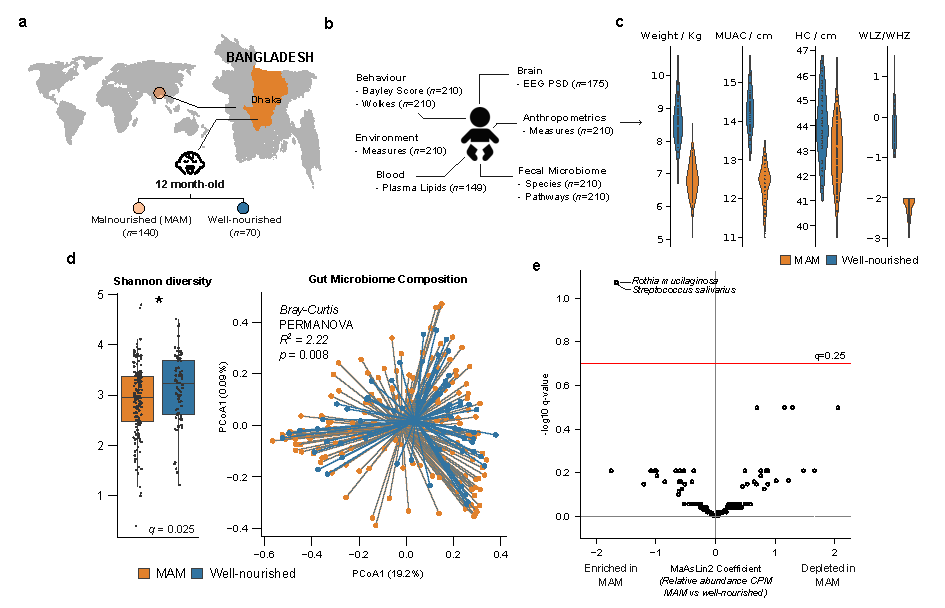
\includegraphics[scale=0.9]{../../figures/Figure1-microbiome.pdf}
\caption[Malnutrition impacts the 12-month-old infant gut microbiome]{
	Malnutrition impacts the 12-month-old infant gut microbiome.
	a) Schematic of study design.
	b) Summary of data collected.
	c) Change in diversity of the gut microbiome associated with malnutrition.
	d) PCoA Scatterplot of Bray-Curtis beta diversities of samples (each marker is a single infant sample).
	e) Barplot of significant taxonomic differences in relative abundance and prevailence between 12-month-old well-nourished and \gls{MAM} samples (\textit{p} \textless{} 0.05).
	f) Boxplot of \gls{P/B} ratio change between study conditions.
	g) Volcano plot of pathways that associate with malnutrition (red and orange horizontal line signifies \textit{q} \textless{} 0.05 and 0.01 respectively. left and right vertical lines represent Log\textsubscript{2}(\gls{MAM}/well-nourished) of -0.1 and 0.1 respectively).}
\label{Figure1}
\end{figure}

\subsection*{Malnutrition impacts brain activity and expressive communication}
Malnourished children often present with long-term impairments in neural and cognitive development \cite{martins2011long}.
The Bayley Scales of Infant and Toddler Development Fourth Edition (BSID-IV; \cite{Bayley2019}) was used to assess development in the cohort.
When compared to well-nourished infants, there was a significant reduction in the Expressive Communication, Fine Motor, and Gross Motor scores in the \gls{MAM} infants (mean difference(\gls{MAM} - well-nourished) = -2.02, -1.68, -2.69, \textit{p} = 0.0036, 0.0005, 0.0082) (\autoref{Figure2}b, \autoref{TableS5}).
Expressive communication is a measure of how well a child communicates with others ().
There was a reduction in all other Bayley metrics including the receptive language, cognitive, motor abilities, but without significance.
To complement this method of assessing development, wolkes scoring was performed for the cohort (\autoref{Figure2}c, \autoref{TableS6}).
As with the Bayley scoring, vocalisation scores were lower in \gls{MAM} infants (mean difference(\gls{MAM} - well-nourished) = -1.47, \textit{p} = 2.05e-10) amongst Activity and Approach scores.

Resting state electroencephalography \gls{EEG} assessments of participants were performed to enable investigation of the impacts of malnutrition on brain activity.
After exploratory comparisons of \gls{EEG} \gls{PSD} between infants with \gls{MAM} and the well-nourished controls, focus on the high-alpha (9-12 Hz), beta (12-30 Hz) and gamma (30-45 Hz) frequency bands distributed across occipital, temporal and frontal regions of interest will be made.
These bands are generally associated with concentration, alertness, and higher mental activity and were observed to have higher amplitudes in the well-nourished infants compared to infants with \gls{MAM} (\autoref{TableS7}).

\begin{figure}[!htb]
\centering
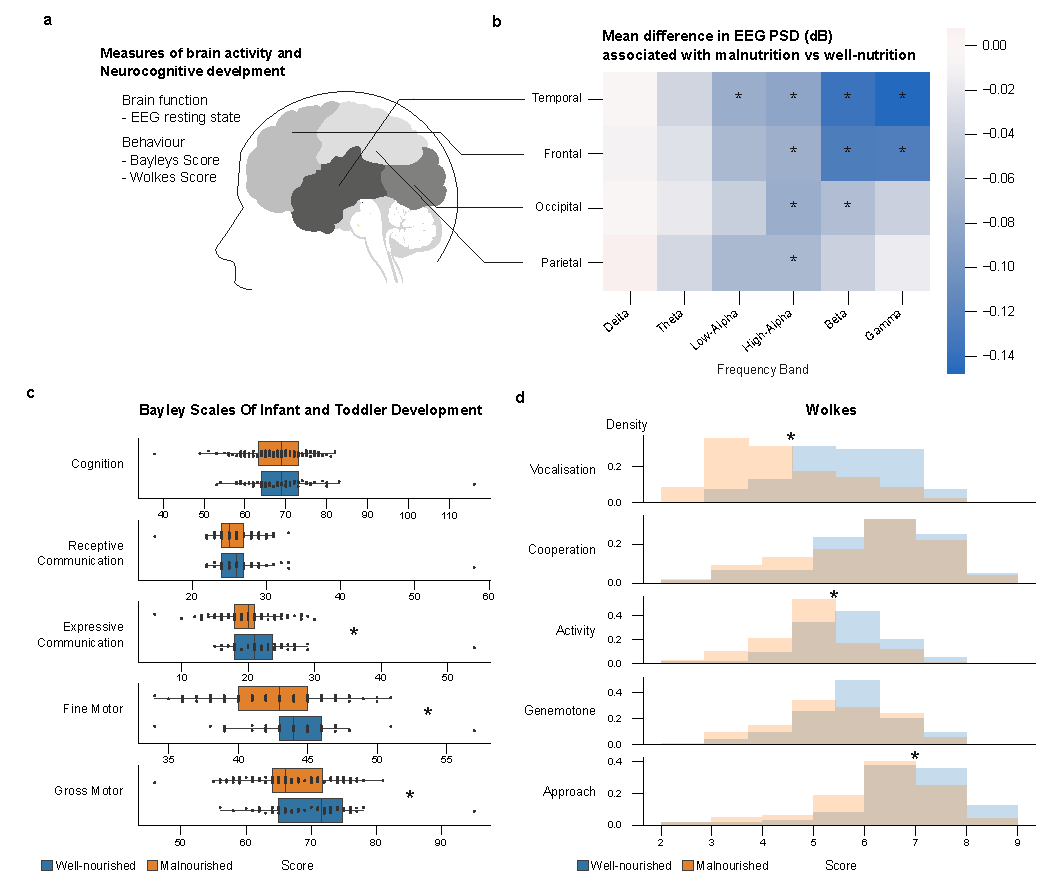
\includegraphics[scale=1.4]{../../figures/Figure2-brain.pdf}
\caption[Differences in cognitive development of 12-month-old infants associate with malnutrition]{
	Differences in cognitive development of 12-month-old infants associate with malnutrition.
	a) Schematic of approach to study neurocognitive function.
	b) Heatmap of lobe and frequency specific changes in EEG resting state power spectral density (PSD) in MAMversus well-nourished infants.
	Distributions of scores identify significant difference in c) Bayley Expressive Communicaiton Score and d) Wolkes Vocalization, Activity and Approach scores of the infants with malnutrition compared to those which are well-nourished.
	* = \textit{q} \textless{} 0.05.}
\label{Figure2}
\end{figure}

\subsection*{Malnutrition is associated with a reduction in circulating odd-chain fatty acids and ceramides}
Adequate nutrition in infants is characterised by healthy circulating concentrations of metabolites, including lipids, involved in growth and development \cite{badaloo2006lipid}.
Delivery of lipids from the gut to the rest of the body is a crucial process during the developmental window.
Therefore, discovery LC-MS/MS was used to assign and quantify the levels of 825 plasma lipids in the infants of the cohort (\autoref{Figure3}).

Malnutrition was associated with major changes (286/825 - 35\%) to the plasma lipidome.
Of these changes, 124 (15\%) plasma lipidome compounds increased and 162 (20\%) decreased in concentration (\autoref{Figure3}, \autoref{TableS8}).
Enrichment in the abundance of three lipid classes with diverse functions was observed, including two that are known to be specific to neurological development and function (ie. the long chain ceramide Cer 31:5;O2 (Log\textsubscript{2}(\gls{MAM}/well-nourished) = 0.36, \textit{q} = 2.12e-7) and the lactosylceramide hex2cer 34:1 (Log\textsubscript{2}(\gls{MAM}/well-nourished) = 0.018, \textit{q} = 0.004)).
By contrast, long chain sphingomyelins (SM 44:3;O2, Log\textsubscript{2}(\gls{MAM}/well-nourished) = FIND, \textit{q} = 5.81e-5)) and others were observed to increase in relative concentration in malnourished infants.
Several lysophospholipids from the lysophosphatidylcholine (LPC), and lysophosphatidylethanolamine (LPE) classes were enriched in well-nourished infant plasma.

\begin{figure}[!htb]
\centering
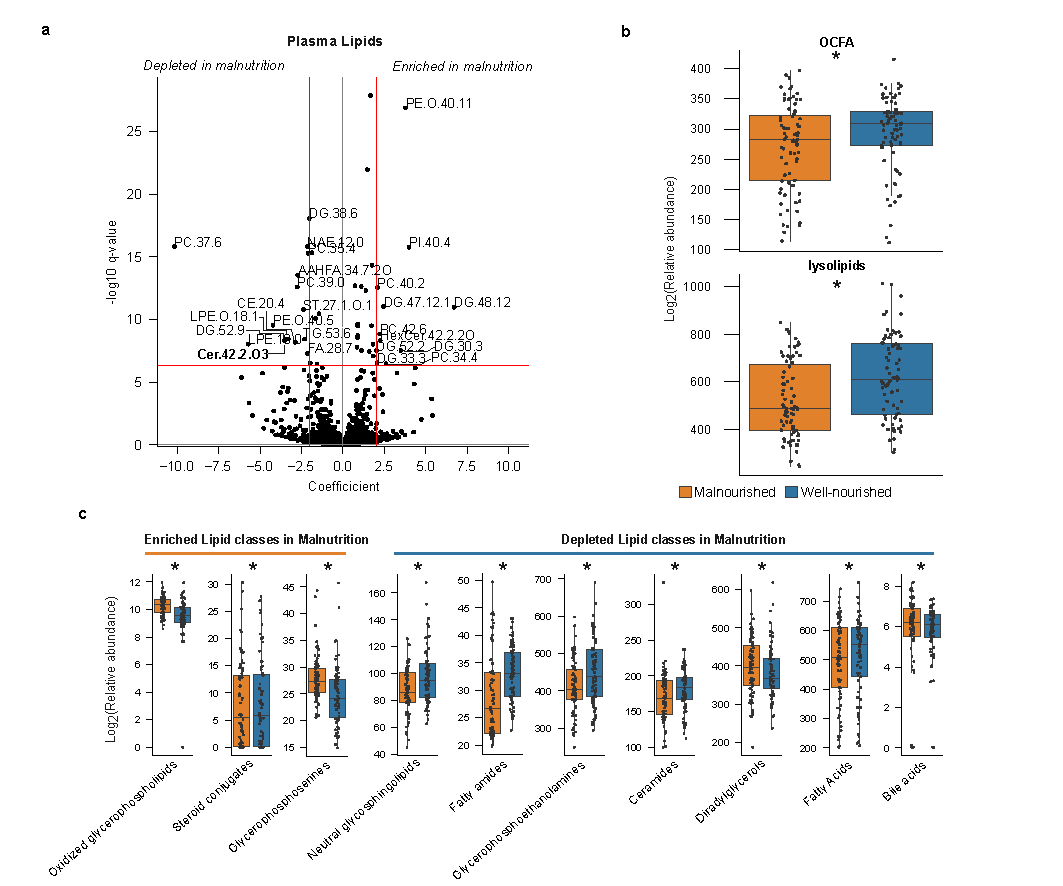
\includegraphics[scale=0.9]{../../figures/Figure3-lipids.pdf}
\caption[Malnutrition results in major compositional differences in plasma lipids in 12-month-olds]{
	Malnutrition results in major, compositional differences in plasma lipids in 12-month-olds.
	Volcano plot changes to plasma lipids between well-nourished and \gls{MAM} 12-month-olds.
	(Upper left and upper right quadrants signify significant changes where the red horizontal line signifies \textit{q} \textless{} 0.05 and vertical lines represent Log\textsubscript{2}(\gls{MAM}/well-nourished) of -0.1 and 0.1 respectively).
	Boxplot of differences in Lysolipid (b) and Ceramide (c) concentrations associated with malnutrition.}
\label{Figure3}
\end{figure}

\subsection*{Multimodal Random Forest classification of malnutrition reveal cross mode influences}
Having established the existence of changes associated with malnutrition across the gut microbiome, brain, and plasma lipids, the relative importance of changes in each of these domains for the prediction of malnutrition was measured.
Individual and multimodal Random Forest classifiers were trained, using gut microbiome taxonomic and functional neuroimaging (EEG), lipidome and behavioural data (Bayley scale scores), to predict malnutrition in the cohort (\autoref{Figure4}).

Within the predictors trained on individual feature sets, plasma lipids (AUCROC=1.00, oob=1.00) were the best predictor of malnutrition in 1-year-old infants, followed by brain/behavioural metrics (i.e., EEG, and Bayley AUCROC=0.83, oob=0.64), and the gut microbiome taxonomic and functional profiles (AUCROC=0.59, oob=0.59).

Ensemble models were trained on individually scaled and combined data from the gut microbiome taxonomic and functional profiles, neuroimaging (EEG), plasma lipidome, and Bayley scale and Wolkes scores and evaluated using AUCROC and 10-fold cross validation.
The ensemble models had an AUCROC of 0.82.

\gls{SHAP} scoring interpretation was performed to understand the workings of these models and importance of the features without the assumption of linearity of relationship (\autoref{Figure4}d, \autoref{TableS9}).
Those features that changed significantly were more likely to have high importance for the model prediction as evident with a spearman correlation between SHAP score and \gls{MWU} -log\textsubscript{2}(\textit{p}) of 0.74.
Comparison with the individual models indicated that inclusion of the other datasets into the ensemble models lead to the identification of non-linear features that contributed to the predictive power of the microbial species within the classification model.
For example, these included \gls{MAM} depleted \textit{Faecalibacerium prausnitzii} (SHAP = 0.0076), and \textit{Odoribacter splanchnicus} (SHAP = 0.0063) or \gls{MAM} enriched \textit{Bifidobacterium breve} (SHAP = 0.0074), and \textit{Haemophilus parainfluenzae} (SHAP = 0.0065).

\begin{figure}[!htb]
\centering
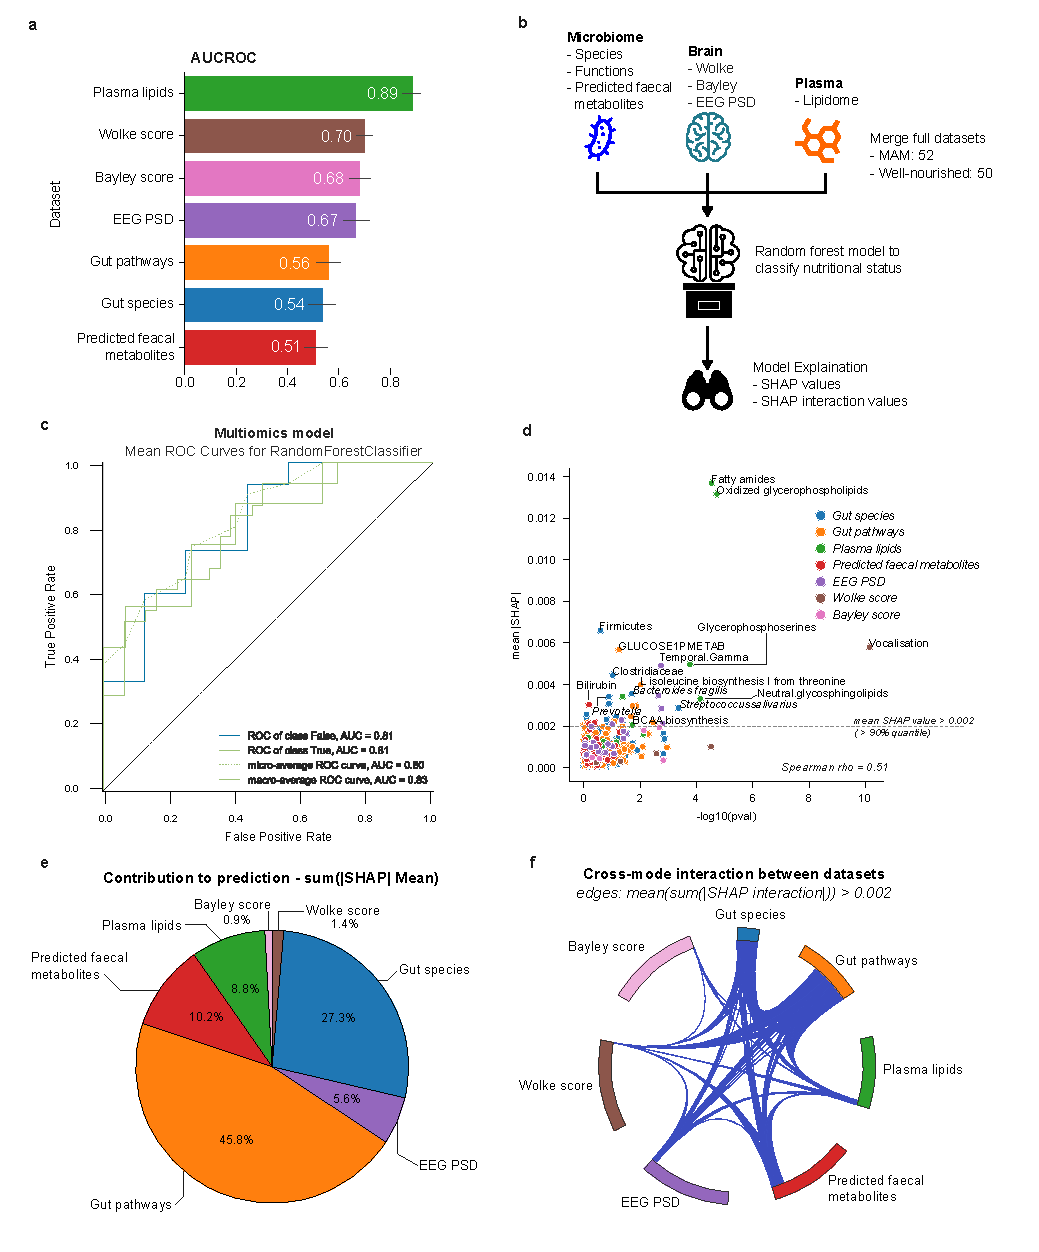
\includegraphics[scale=0.9]{../../figures/Figure4-ai.pdf}
\caption[Integration of multimodal datasets boosts the predictive power and affects the relative feature importance of random forest models predicting nutritional status]{
	Integration of multimodal datasets boosts the predictive power and affects the relative feature importance of random forest models predicting nutritional status.
	a) Schematic describing interpreted multimodal approach to predict malnutrition.
	b) AUCROC curves showing relative predictive power of each modal dataset on predicting nutritional status.
	c) Multimodal model predicts malnutrition accurately.
	d) The multimodal model captures non-linear interactions between the features as demonstrated by the SHAP score distribution.}
\label{Figure4}
\end{figure}

\subsection*{A Multimodal Predictive Network Analysis reveals the importance of \textit{Bacteroides fragilis} in infant neurocognitive development}
Network analysis is a useful tool to understand complex systems that emerge from interactions between multiple components.
To better understand the complexities of the important features and correlations between EEG PSDs, behavior, gut microbial species and functions, and plasma lipids, their architecture was mapped out using co-abundant network analysis (\autoref{Figure5}).
Spearman correlation of the features that were important in predicting malnutrition was calculated, and filtered by significance (\textit{q} = \textless{}0.05) (1052/3906 correlations,  \autoref{TableS10}).

Important features (ie. mean absolute \gls{SHAP} score \textgreater{} 0.002 (above 85\%)) were more likely to be significantly correlated (q \textless{} 0.05) with one another and had greater measures of Betweenness Centrality (\autoref{Figure5}, Supplementary Table X) than unimportant features (mean absolute \gls{SHAP} \textless{} 0.002).
Plasma lipids that were enriched/depleted in the \gls{MAM} condition (Supplementary Table X) were positively correlated with the anthropometric measures \gls{WLZ/WHZ}, \gls{MUAC}, and weight.
Unsurprisingly, cluster analyses revealed that those features which were different between \gls{MAM} and well-nourished were positively correlated with each other (i.e., change in the same direction, supp table).
A subcluster of \textit{B. fragilis}, pyruvate fermentation pathways, plasma ceramides, EEG PSD and Expressive Communication was identified that was highly correlated with the well-nourished state (\autoref{Figure5}).
Those plasma lipids that were depleted (\textit{q} \textless{} 0.05, Log2(\gls{MAM}/well-nourished) \textless{} 0) from the \gls{MAM} infant samples were also positively correlated with EEG PSD amplitudes.
Notably, EEG metrics were also correlated with bacterial pyruvate fermentation pathways and \textit{B. fragilis} relative abundance.
Conversely, a correlated subcluster of \textit{P. copri}, glycolysis, peptidoglycan biosynthesis, BCAA pathways, and plasma sphingomyelins that were associated with the \gls{MAM} condition was identified. 

\begin{figure}[!htb]
\centering
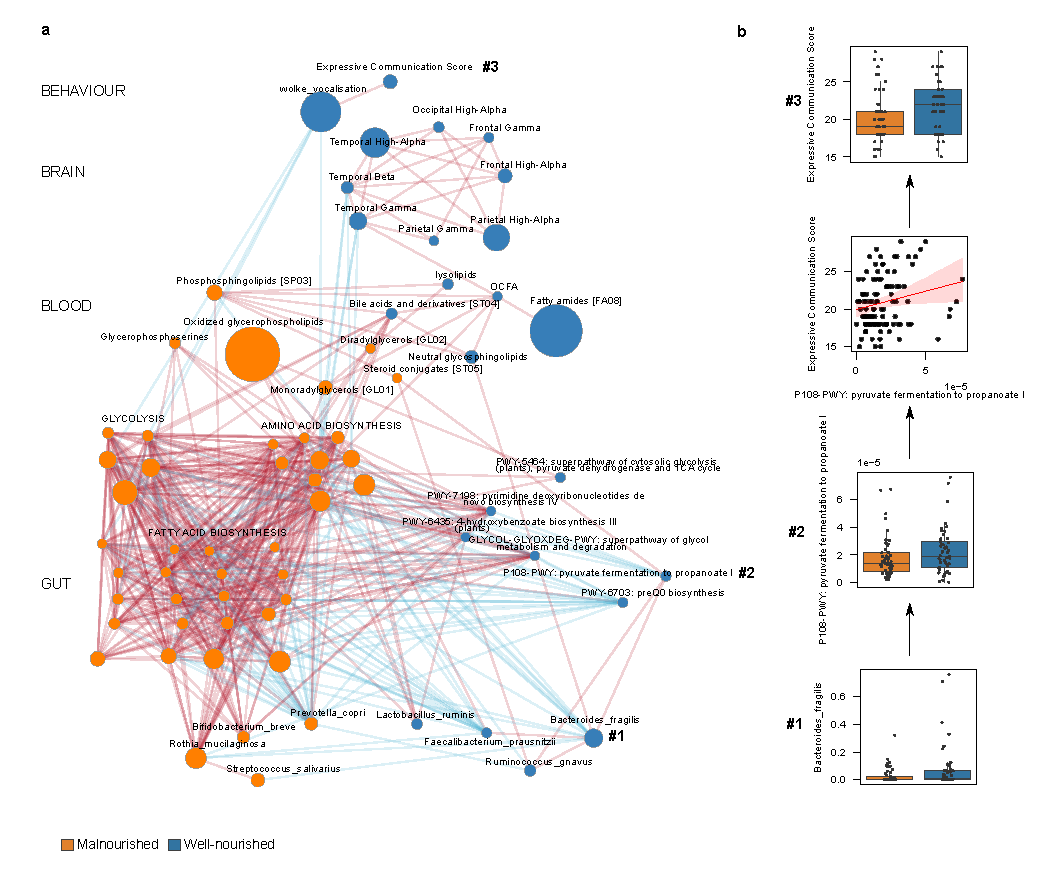
\includegraphics[scale=0.9]{../../figures/Figure5-network.pdf}
\caption[\textit{Bacteroides fragilis} forms a network with propanoate synthesis, EEG and expressive communication that is anti-correlated with a \textit{P. copri} focused cluster of features in healthy and malnourished individuals]{
	\textit{Bacteroides fragilis} forms a network with propanoate synthesis, EEG and expressive communication that is anti-correlated with a \textit{Prevotela copri} focused cluster of features in healthy and malnourished individuals.
	a) Network illustrating inter-relationships of feature associations that predict malnutrition.
	Inclusion in the network requires both a SHAP score for the node (\textgreater{} 0.6) and a significant Spearman rho score for the correlation of \textit{q} \textless{} 0.05.
	Nodes are features coloured by their enrichment in \gls{MAM} (orange and green are enriched and depleted in \gls{MAM} respectively).
	Edges are spearman correlations coloured red and blue being positively and negatively correlated respectively.
	b) Evidence for relative abundance of \textit{B. fragilis} (\#1), pyruvate fermentation to propanoate I pathway relative abundance (\#2), correlation between pyruvate fermentation to propanoate I pathway and Expressive communication, Expressive communication score distributions (\#3).}
\label{Figure5}
\end{figure}

\section*{Discussion}
A central goal of this study was to obtain a better understanding of how disturbances in host-microbiome interactions impact neurocognitive development in malnutrition.
It was observed that malnutrition was characterised by a higher \gls{P/B} ratio and reduced pyruvate fermentation potential in the gut.
\textit{Prevotella} rich microbiomes (previously referred to as the Prevotella enterotype) have been typically understudied due to their underrepresentation in non \gls{LMIC} \cite{tett2019prevotella}.
This ratio has previously been implicated in diet and lifestyle, particularly in adults \cite{hjorth2019prevotella} and \textit{Bacteroides} have been observed previously to be depleted in Bangladesh infants \cite{roger2022impact}.
Other studies of malnutrition have shown similar reductions in alpha diversity \cite{roger2022impact}.
Accelerated ageing of the gut microbiome, as indicated by the presence of specific markers such as \textit{P. copri} and \textit{Bifidobacterium adolescentis}, is one possible hypothesis for the differential \textit{Prevotella} abundance.
This could indicate that the development of the microbiome-gut-brain axis is pathologically accelerated during infant malnutrition.
Alternatively, selective microbiome community driven interactions might explain the inverse correlations that were observed between \textit{P. copri} and \textit{Bifidobacterium} species.
\textit{B. longum} and other anaerobic species have been previously linked to moderate and severe acute malnutrition in Bangladesh \cite{barratt2022bifidobacterium,  million2016increased}.

Comparisons of the \gls{MAM} and control infants identified deficits both in brain electrical activity and expressive communication that were associated with malnutrition.
Severe acute malnutrition during childhood is generally recognized as having long-term effects on adult cognitive, academic and behavioral development \cite{mwene2020long}.
Despite this, our integrated analysis did not identify any significant ‘direct’ correlations between brain EEG and behavioral measures (Wolkes vocalization and Baley expressive language) in malnourished one year old children.
When investigating differences in EEG activity, disruptions were evident for higher frequency power bands (alpha, beta, and gamma) but not lower frequency bands (delta and theta) in frontal, temporal and occipital areas.
Notably, we did identify connections between the gut microbiome, microbial pathways and the blood metabolome and either behavioral measures or brain electrical activity (EEG measures).
It is clear that brain development (e.g. white matter volume) and learning and motor functions are associated with age and affected by malnutrition \cite{fields2008white, galler2021neurodevelopmental}.
However, there is no reason to assume that effects on complex behaviors are realized through alterations in electrical activity (e.g. power) within the synchronously firing neuron populations, which instead represent the early stages of information processing.
Rather, there are moderating factors (extreme poverty, prenatal factors, maternal education, and family interactions) that provide considerable explanatory power for this widely recognized association with early childhood development \cite{alam2022early}.
Indeed, previous analyses of data from the national-scale dataset from Bangladesh Multiple Indicator Cluster Survey in Bangladesh have identified that children of educated mothers and ‘solvent’ households exhibited better early childhood development.
Notably, our analysis separated the impact of these, connecting Mother’s occupation to the EEG signal – and early stage learning, father’s occupation to measures of solvency (sanitation, owning a clock, shared toilet) and the child’s microbiome, consistent with a separation of pathways for behavioral and brain development.  

We identified significant differences in plasma lipids within the malnourished children.
These changes included both increases and decreases in polyunsaturated fatty acids (PUFA) with extended chain lengths (\textgreater{}18) or odd chain numbers (e.g. ...).
The observed reductions may be trivially interpreted as indicating the combined effects of reduced dietary intake (e.g. C16 and C18 derivatives) and altered microbial metabolism (e.g. odd chain FA) in the malnourished condition.
By contrast, the increased largely very long chain fatty acids (> C20) likely reflects an alteration in host metabolism.
This is consistent with observations that low protein diet induced malnutrition in rats results in hepatic steatosis, loss of peroxisomes and mitochodrial dysfunction \cite{van2016malnutrition}.
Peroxisomes are important for \textbeta{}-oxidation of very long chain fatty acids (\textgreater{}C20), branched fatty acids, xenobiotics and bile acids.
The low protein diet peroxisome and mitochondrial dysfunction is is reflected in severe metabolic disruption including to the levels of plasma lipids, consistent with our observations in the malnourished individuals.
The malnutrition associated reduction in 16C and 18C chain FA may reflect the dietary deprivation.
Notably, the plasma lipidomes of malnourished children also exhibited significant differences in the levels of ceramides and lysolipids (i.e. lipid derivatives in which one or both acyl derivatives have been removed by hydrolyisis).
Numerous specific changes stand out as being potentially important for neural development.
Firstly, lactosylceramide (hex2cer 34:1) is an essential precursor for synthesis of all complex glycosphingolipids \cite{d2013glycosphingolipids} that was depleted by approximately 50\% in malnourished infants.
Secondly, lysophosphatidylcholine (LPC) and lysophosphatidlylethanolamine (LPE) are essential for brain development and growth as they carry fatty acid across the blood-brain barrier, via the major facilitator superfamily domain-containing protein 2A (Mfsd2a) \cite{tan2020emerging}.
Phosphatidylcholine (PC) is a precursor to acetylcholine, an essential neurotransmitter for memory and cognitive function.
Supplementing neuron differentiation medium with phosphatidylcholine reduces the impact of inflammatory stress and neuronal damage, increasing the numbers of healthy neurons and modulating neuronal plasticity \cite{magaquian2021phosphatidylcholine}.
By contrast, PI 40:4 increased within the plasma of malnourished children.
PI 40:4 s a precursor to prostaglandin synthesis that is important for brain development (PMC3521678).
The associations between microbial fatty acid biosynthesis, plasma lipids and electrical activity in the brain may relate to processes about myelin biosynthesis and maintenance, as has been previously proposed \cite{nunez2015eeg}.
However, further work is required to test this hypothesis. 

The integrated analysis identified a non-linear association for circulating bile acids with the microbiome and, through phosphosphingolipids, behavioural outcomes (i.e. Wolkes vocalization and Bayley expressive communication).
This reflected a non-significant trend to increase bile acid concentrations within the serum of malnourished children.
Exactly what the bile acid association with phsophosphingolipds reflects is unclear.
However, bile acids are hormone like molecules that have recognized, albeit poorly described, roles as signalling molecules to the brain (reviewed in \citet*{hurley2022bile}).
Secondary bile acids are synthesized directly by the microbiome and are detectable in the brain where there are numerous bile acid receptors \cite{hurley2022bile}.
Notably, deletion of the Farnesoid X receptor (FXR), involved in bile acid homeostasis, was associated with a reduction in depressive and anxiety-like behaviour, but increased motor activity.
Collectively, these findings reinforce the hypothesis that there is microbial signalling, through the peripheral circulatory system to the brain that is capable of impacting on behaviour.
However, direct causal effects are yet to be demonstrated for the compounds we have identified \cite{huang2015deletion}.
Random Forest classification models trained on the gut microbiome, neuroimaging data, and the plasma lipidome accurately predicted the malnutrition condition.
Integrating the important features of these models and Spearman correlation using network analysis provided a holistic view of the malnutrition mechanism and highlights the potential importance of a susbset of microbes (i.e. \textit{Bacteroides fragilis}) as a indicators of infant neurocognitive and microbiome-gut-brain axis development in malnutrition. 

Recent studies have emphasised the significant role of the gut microbiome in mediating dietary effects on host physiology, in addition to its influence on the development and function of the nervous system \cite{heiss2019role, ceppa2019current, marques2014gut, fung2017interactions}.
Multiomics analysis examined associations between infant malnutrition, altered brain function, and the infant microbiome and revealed a mechanism that links the fermentation of pyruvate to butanoate and ceramide biosynthesis to brain function and language development.
However, in the absence of causal animal studies, it remains unclear if the gut microbiome, and plasma metabolite changes are a result of, or contribute causally to the wider malnutrition phenotype. 
This study is not without limitations.
Several of the limitations are linked to the cross-sectional cohort itself and lack of temporal samples, the correlative nature of the data, and choice of measures (e.g. EEG for electrical conductivity, as a measure of brain development).
Notwithstanding these limitations the integrated dataset and incorporation of age matched controls, provide evidence that clearly supports emergent hypotheses that require subsequent testing in animal models and within the on-going clinical trial that this cohort is participating in.

\section*{Conclusion}
Integrative multi-omics highlight inter-connected pathways between features of gut microbiome, microbial metabolism, plasma lipids and either brain connectivity (EEG) or cognitive function.
These pathways provide testable hypotheses to optimise malnutrition associated behavioural and brain development changes. 

\section*{Methods}
\subsection*{Ethics}
The M4EFaD intervention was registered NCT05629624 on clinicaltrials.gov.
The study was approved by icddr,b Ethical Review Committee PR-21084 and the Bangladesh Directorate General of Drug Administration.
Ethical review for the analytical component was obtained from Auckland Health Research Ethics Committee approval AH23922 (metabolomics, metagenomics, machine learning).

\subsection*{Study Design and Participants}
The study was performed on the baseline data from three cohorts of infants who were enrolled (between Jan – December 2022) as part of the M4EFaD intervention within the Mirpur slum, Dhaka, Bangladesh.
The cohort consisted of: a control group of 73 well-nourished children at 12 ± 1 months (WLZ z-score \textgreater{} -1 SD); an intervention group of 156 children with WLZ \textless{} -2 and \textgreater{} -3 z-score, and/or MUAC \textless{} 12.5 and \textgreater{} 11.5 cm having \gls{MAM} at 12 ± 1 months; and an outcome reference group of 73 children with WHZ \textless{} -2 and \textgreater{} -3 z-score, and/or \gls{MUAC} \textless{} 12.5 and \textgreater{} 11.5 cm having stable \gls{MAM} at 3 years ± 2m.
Inclusion criteria included a diagnosis of malnutrition, no history of chronic medical conditions, and no antibiotic use within the past month.
The study protocol has been submitted for publication and is available on MedRxiv \cite{shama2023multidimensional}.

\subsection*{Recruitment and anthropometric data collection}
Enrolment was initiated on February 7, 2022, and will continue until February 2024.
Study surveillance workers (SWs) conducted a door-to-door census (approximately 100,000 households) in Mirpur DNCC wards ward 2, 3 and 5 between January and December 2022.
Verbal consent was obtained to participate in the census.
The census identified 5736 children aged between 11 to 13 months and 2,314 children aged between 34 to 38 months.
During the census, if the guardian verbally consented to the study procedure, and the babies met the inclusion and exclusion criteria of the study (Table 1), the SWs proceeded to measure the \gls{MUAC} of the child.
Mothers of babies who were within the \gls{MUAC} range were invited to visit the icddr,b study clinic for further assessment and enrolment.

Final screening for eligibility and study consent occurred at the icddr,b Mirpur study clinic.
The consenting process was tailored to each mother's literacy level and involved reviewing the inclusion and exclusion criteria.
Comprehension of the study was assessed using scripted points and open-ended questions.

Following consent, the clinical screening team completed a screening form, capturing the date of enrolment, sex, date of birth (DOB), weight (in kg), length/ height (in cm), head circumference (in cm), and Mid-Upper Arm Circumference \gls{MUAC} measurements of the child.
The \gls{WLZ/WHZ} Z-score for each child was calculated using the WHO anthropometric calculator.
The child's age was validated using the EPI vaccination card.
Neurological measures, Bailey scores, EEG data were collected upon enrolment to evaluate neurological development.

\subsection*{EEG data collection and analysis}
Continuous scalp EEG was recorded using NetStation 4.5.4. and 128-channel Hydrocel Geodesic Sensor Nets modified to remove eye electrodes (Electrical Geodesics, Inc. (EGI), Eugene, OR, USA).
Data was sampled at 500 Hz.
Impedances were kept under 100 k \textomega{} when possible and measured once at the beginning of the session, and again halfway through.
Sessions were conducted in a dimly lit room with the participants sitting on the parent’s lap.
The participants were separated from the research staff conducting the session by a curtain, but the testing area was not acoustically or electrically shielded.
A second research staff member was present in the testing area to help keep the participant engaged.
EEG sessions consisted of 6 paradigms, i.e., resting state, visual working memory, flanker, disengagement, visual evoked potential, and auditory stimuli.
The subsequent (pre-)processing steps were applied to the resting state data where participants watched a 3-minute video that featured toys.

EEG data were preprocessed offline with MatLab (R2021B) using the Harvard Automated Processing Pipeline for Electroencephalography (HAPPE) Version 3 (Gabard-Durnam et al., 2018).
A specified subset of 30 channels was excluded (‘E1’, ’E8’, ’E14’, ’E17’, ’E21’, ‘E25’, ’E32’, ‘E38’, ‘E43’, ’E44’,’ E48’, ’E49’, ’E56’, ’E63’, ’E68’, ’E73’, ’E81’, ’E88’, ’E94’, ’E99’, ’E107’, ’E113’, ’E114’, ’E119’, ’E120’, ’E121’, ‘E125', 'E126', 'E127', 'E128').
Data were downsampled to 250Hz, bandpass filtered (1-100Hz), and filtered using a 50Hz cleanline filter for line noise removal.
Bad channels were then automatically identified and rejected, and wavelet-enhanced Independent Component Analysis (ICA) and the Multiple Artifact Rejection Algorithm (MARA) were performed to detect and impute artifacts.
Resting state data were segmented into 2s epochs; epochs with an amplitude >±150mV were rejected.
Segments were also rejected using segment similarity criteria.
Data were then re-referenced to the average of all channels.

EEG outputs from HAPPE were then reformatted and processed using the Batch Electroencephalography Automated Processing Platform (BEAPP) (Levin et al., 2018) to extract power spectra for each participant across the following frequency bands: delta (2-4Hz), theta (4-6Hz), low alpha (6-9Hz), high alpha (9-12Hz), beta (12-30Hz), and gamma (30-45Hz) and the following regions of interest (see Supp Figure 2): occipital (‘E70’, ’E71’, ’E75’, ‘E76’, ‘E83’), temporal (‘E36’,‘E40’, ‘E41’, ‘E45’, ‘E46’, ‘E102’, ‘E103’, ‘E104’, ‘E108’, ‘E109’), parietal (‘E52’, ‘E53’, ‘E59’, ‘E60’, ‘E85’, ‘E86’, ‘E91’, ‘E92’), and frontal (‘E5’, ‘E6’, ‘E12’, ‘E13’, ‘E24’, ‘E27’, ‘E28’, ‘E33’, ‘E34’, ‘E112’, ‘E116’, ‘E117’, ‘E122’, ‘E123’, ‘E124’).
Further, PSD values were normalized by a Log\textsubscript{10} transform.

\subsection*{Developmental Outcomes (Bayley)}
The Bayley Scales of Infant and Toddler Development, Fourth Edition (BSID-IV) cognitive, language, and motor subscales were administered to all participants.
Research assistants were trained to research reliability in the administration and scoring of the Bayley-4.
Due to cultural differences between the Bangladesh and the United States where the assessment was developed, Bangladeshi researchers modified some assessment stimuli to improve cultural responsiveness and relevancy.
For example, pictures for the item naming series and action naming series of the expressive language and receptive language subscales were adapted to include items that Bangladeshi children are more likely to be familiar with and bedtime clothing that would signify the child in the picture was going to sleep instead of the one-piece pajamas worn in the original picture, which the Bangladeshi children would not be familiar with. 
SECTION ON WOLKES.

\subsection*{Biological sample collection}
Stool samples were collected from each infant at their home at the baseline visit.
Samples were collected in DNA/RNA Shield Fecal Collection Tubes (Zymo Research, \#R1101).
Peripheral venous blood samples were collected in EDTA Vacutainers, separated into plasma and RBCs and immediately frozen at -80 C.
Batches of blood and stool samples were air-freighted on dry ice from Bangladesh to the Liggins Institute, New Zealand for processing and analysis. 

\subsection*{Microbiome DNA extraction and sequencing}
DNA was extracted from stool samples using the ZymoBIOMICS MagBead DNA/RNA extraction kit (Zymo Research, \#R2136) following the standard protocol.
Samples (1 mL) were mechanically lysed in bead bashing tubes using the MiniG tissue homogenizer prior to extraction of DNA.
200 µL of the sample was used post-bead bashing for extraction of DNA following the protocol.
A volume of 50 \textmu{} L of elute was collected in DNAse/RNAse Free Water.
Samples with a DNA concentration \textless{} 14.5 ng/\textmu{}L were re-extracted following the ZymoBIOMICS DNA extraction protocol.
Samples were sequenced (Illumina NovaSeq 150PE reads) to an average sequencing depth of 20M read-pairs/sample.
Raw sequences were processed using BioBakery3 tools \cite{beghini2021integrating}, specifically read quality filtering and human decontamination with KneadData (Version 1), taxonomic profiling with MetaPhlAn3 (Version 3.1, using the mpa\_v31\_CHOCOPhlAn\_201901 database) and functional profiling using presence/absence and abundance of microbial pathways (MetaCyc) with HUMAnN3 (Version 3.6).
A minimum threshold of \textgreater{} 0.1\% relative abundance and \textgreater{} 5\% prevalence for all detected species was applied. 

\subsection*{Plasma lipidomics}
Plasma samples for lipidomics were thawed on ice and extracted according to a method modified from \citet*{liu2016plasma}.
Briefly, 10 \textmu{}L volume was placed in an amber glass autosampler vial and 300 \textmu{}L of a mixture of Type 1 water, butanol, methanol, chloroform and SPLASH Lipidomix in a ratio of 4:15:15:20:1 was added.
The mixture was vortexed and sonicated at room temperature before the protein precipitate was removed by centrifugation and an aliquot of supernatant transferred to an amber glass autosampler for negative ionisation LC-MS/MS.
A second aliquot of supernatant was diluted 5 times with 75\% IPA for positive ionisation LC-MS/MS.
A 5 µL volume of each sample was injected onto a Phenomenex Kinetex F5 column (100 mm × 2.1 mm × 2.6 \textmu{}m) and lipids were separated using a ternary gradient of Type 1 water, methanol and isopropanol containing ammonium acetate.
Lipids were quantified and identified with a Q-Exactive mass spectrometer (Thermo Fisher Scientific, Germany) equipped with a heated electrospray ionisation HESI source.
Data was processed using MS-DIAL v4.92 92 \cite{tsugawa2015ms}.
For full methodological details see the supplementary information.

\subsection*{Statistical Analyses}
Python version 3.9.2 was used to perform all analysis \cite{van1995python}.
Due to the unequal sample sizes and non-normally distributed data; non-parametric statistical approaches were used for differential abundance analysis.
Relative abundances were adjusted by Centred Log Ratio to account for the compositional nature of the dataset \cite{gloor2016s}.
Log adjusted fold change significance was measured using (\gls{MWU}) test using the ‘mannwhitneyu’ function from ‘scipy.stats’ and adjusted for multiple testing using the ‘fdrcorrection’ function from statsmodels.stats.multitest.
\gls{PCoA} ordinations (plotted using 'skbio.stats.ordination.pcoa' module) were used to visualise the clustering of the Bray-Curtis dissimilarities (calculated using skbio.distance.pdist) between samples from their species and functional composition.
To quantify the variance of the gut microbiome explained covariates, \gls{PERMANOVA} p-values were calculated from those Bray-Curtis Dissimilarities using the ’permanova’ function from the 'skbio.stats.distance' module.
Bray-Curtis were also used to capture the temporal dynamics of the microbiome from baseline.
Numerical Associations between species and metadata were measured with Spearman correlation (calculated using 'spearmanr' function from 'scipy.stats' module), where significance was defined as \gls{FDR} adjusted p-values of \textless{} 0.05 as per \citet*{2020SciPyNMeth}.
Associations between categorical data were measured with Fisher's Exact test (calculated using 'fisher\_exact' from 'scipy.stats' module), where significance was defined as p-values of \textless{} 0.05.

\subsection*{Machine learning}
Machine learning models were used to classify malnourished from well-nourished infants.
Extra-trees Random Forest models were trained on functional and microbial taxa relative abundances.
Model hyperparameters including the number of trees in the forest, maximum tree depth, and minimum sample numbers needed to split internal nodes were tuned using grid searching.
A 5-fold cross-validation was used to measure the performance of each hyperparameter combination and to identify overfitting.
Model performance was measured with AUCROC and out-of-bag error analysis (oob).
SHAP Value (SHapley Additive exPlanations) interpretation was used to interpret the contributions each feature had on the model's performance using the ‘shap’ python package \cite{lundberg2017unified}.

\subsection*{Network analysis}
Absolute spearman rho of above 0.3 were used as edges and gut bacterial species and functional profiles, EEG, and plasma lipids were used as nodes coloured by their mean SHAP scores for classifier models that distinguish \gls{MAM} from well-nourished conditions.

\section*{Code availability}
All analysis code is available on the GitHub repository.
The codebase is organised into scripts, providing a comprehensive framework for replicating the experiments.
Detailed documentation and instructions on how to use the code are provided in the repository's README file.

\section*{Ethics approval and consent to participate}
Ethical approvals were obtained from the Research Review Committee (RRC; August 21, 2021) and Ethical Review Committee (ERC) of icddr,b (protocol no: PR-21084; September 21, 2021), Institutional Review Board of Boston Children’s Hospital, USA (for analyses of neuropsychological assessments), University of Auckland, New Zealand (approval AH23922; for analyses of collected biological samples) and University of West Indies (CREC-MN.51, 21/22).

\section*{Data availability}
Metagenome data is available at PRJNAXXX on the SRA. 
EEG and metadata are available from the authors, upon reasonable request that meets the ethics of the study.

\section*{Competing interests}
The authors declare that they have no competing interests.

\section*{Funding}
Work on this clinical trial is supported by Wellcome Leap (9942 Culver Blvd Unit 1277 Culver City, CA 90232-4167, United States; www.wellcomeleap.org) to PDG, JMO, TF and CAN as part of the 1kD Program.
We acknowledge our core donors, Governments of Bangladesh, Canada for providing unrestricted support and commitment to icddr,b's research effort.

\section*{Author Contributions}
TP, KG and JOS drafted and co-wrote the manuscript.
TS, SHK, BCW, BH, CP, AB, DH, IS, AME, RD, GG, CK, PDG, RH, TF, CAN commented on the manuscript.
JMO, RH, TF, PDG, CAN designed the study and analyses.
TS, SHK performed assessments and obtained samples in Dhaka.
RH oversaw the Dhaka group.
TP performed multiomic analyses, BCW and IS performed metagenomics, CP performed metabolomics, JOS oversaw the Auckland group.
BH performed EEG analyses, CAN oversaw the Boston group.

\section*{Acknowledgements}
The authors would like to acknowledge the participants in Mirpur, Dhaka, Bangladesh for their contributions to this study.
The authors would also like to thank the study team within the Infectious Diseases Division, International Centre for Diarrheal Disease Research, Bangladesh for their work in participant recruitment, sample collection and assessments.

\bibliography{library}
%\printbibliography

\section*{Supplementary material}

\begin{table}[!htb]
\centering
\caption[Baseline infant characteristics]{
	Baseline infant characteristics.
	Plus minus values are means \textpm{} SD from continous variables and their pvalues are calculated using \gls{MWU}.
	All other variables are categorical (True vs False) with their pvalues calculated using Fishers Exact test.}
%\begin{longtable}{llll}
\toprule
 & Malnourished & Well-nourished & qval \\
target &  &  &  \\
\midrule
\endfirsthead
\toprule
 & Malnourished & Well-nourished & qval \\
target &  &  &  \\
\midrule
\endhead
\midrule
\multicolumn{4}{r}{Continued on next page} \\
\midrule
\endfoot
\bottomrule
\endlastfoot
WLZ\_WHZ & -2.24 ± 0.26 & -0.23 ± 0.48 & <0.001 \\
MUAC & 12.4 ± 0.49 & 14.26 ± 0.6 & <0.001 \\
Weight & 6.8 ± 0.52 & 8.58 ± 0.69 & <0.001 \\
HC & 42.98 ± 1.33 & 43.97 ± 1.35 & <0.001 \\
Principal\_type\_of\_toilet\_facility\_used\_by\_household\_members.Septic tank or toilet & 106/159 (66.7\%) & 68/75 (90.7\%) & 0.002 \\
Water\_treatment\_method.Boil & 70/159 (44.0\%) & 51/75 (68.0\%) & 0.018 \\
Father’s\_occupation.Businessman (> 30,000 Tk./ Month) & 0/159 (0.0\%) & 6/75 (8.0\%) & 0.023 \\
Principal\_type\_of\_toilet\_facility\_used\_by\_household\_members.Pit latrine & 40/159 (25.2\%) & 6/75 (8.0\%) & 0.032 \\
Delivery\_Mode.Vaginal & 104/159 (65.4\%) & 35/75 (46.7\%) & 0.106 \\
Delivery\_Mode.Caesarean & 55/159 (34.6\%) & 40/75 (53.3\%) & 0.106 \\
Number\_of\_years\_lived\_in\_current\_household & 5.39 ± 6.28 & 3.83 ± 5.22 & 0.135 \\
Toilet\_facility\_shared\_with\_other\_households & 129/159 (81.1\%) & 49/75 (65.3\%) & 0.157 \\
Mother’s\_income\_taka & 1425.79 ± 3108.0 & 600.0 ± 2046.75 & 0.177 \\
Years\_of\_father's\_education & 4.96 ± 3.67 & 6.45 ± 4.29 & 0.201 \\
Father’s\_occupation.Daily labourer (unskilled labourer) & 38/159 (23.9\%) & 8/75 (10.7\%) & 0.218 \\
Water\_treatment\_method.Water filter & 6/159 (3.8\%) & 9/75 (12.0\%) & 0.226 \\
Type\_of\_cooking\_fuel.Wood & 22/159 (13.8\%) & 3/75 (4.0\%) & 0.231 \\
Mother’s\_occupation.Housewife & 117/159 (73.6\%) & 65/75 (86.7\%) & 0.264 \\
Monthly\_total\_expenditure\_taka & 14854.4 ± 6388.11 & 18469.33 ± 10791.88 & 0.284 \\
Language.Bangali & 146/159 (91.8\%) & 74/75 (98.7\%) & 0.335 \\
Language.Urdu & 13/159 (8.2\%) & 1/75 (1.3\%) & 0.335 \\
Principal\_type\_of\_toilet\_facility\_used\_by\_household\_members.Water-sealed or slab latrine & 13/159 (8.2\%) & 1/75 (1.3\%) & 0.335 \\
Uses\_social\_media.False & 109/159 (68.6\%) & 41/75 (54.7\%) & 0.339 \\
Uses\_social\_media.Regular & 34/159 (21.4\%) & 25/75 (33.3\%) & 0.392 \\
Mother’s\_occupation.Garments worker & 9/159 (5.7\%) & 0/75 (0.0\%) & 0.418 \\
Place\_for\_cooking\_for\_household.Outdoors & 100/159 (62.9\%) & 38/75 (50.7\%) & 0.517 \\
Maid\_working\_in\_household & 1/159 (0.6\%) & 3/75 (4.0\%) & 0.541 \\
Washing\_-\_agent\_used\_after\_defecating.Soap & 133/159 (83.6\%) & 69/75 (92.0\%) & 0.553 \\
Washing\_-\_agent\_used\_after\_defecating.Water & 26/159 (16.4\%) & 6/75 (8.0\%) & 0.553 \\
Place\_for\_cooking\_for\_household.Inside house & 58/159 (36.5\%) & 36/75 (48.0\%) & 0.584 \\
Sex\_of\_the\_Child.Female & 77/159 (48.4\%) & 28/75 (37.3\%) & 0.601 \\
Sex\_of\_the\_Child.Male & 82/159 (51.6\%) & 47/75 (62.7\%) & 0.601 \\
Ethnicity.Bihari & 16/159 (10.1\%) & 3/75 (4.0\%) & 0.614 \\
Ethnicity.Bengali & 143/159 (89.9\%) & 72/75 (96.0\%) & 0.614 \\
Family\_expenditure\_food,\_clothes,\_utility\_bills\_i.e.\_electricity,\_gas,\_water\_taka\_ & 10084.91 ± 4770.1 & 12080.0 ± 7590.02 & 0.625 \\
Birth\_order\_of\_enrolled\_child\_among\_live\_births & 1.79 ± 0.99 & 1.59 ± 0.81 & 0.712 \\
Mother’s\_occupation.Daily labourer (unskilled labourer) & 6/159 (3.8\%) & 0/75 (0.0\%) & 0.721 \\
Washing\_-\_method\_used\_after\_defecating.Left hand & 5/159 (3.1\%) & 6/75 (8.0\%) & 0.722 \\
Place\_of\_birth.Clinic & 97/159 (61.0\%) & 53/75 (70.7\%) & 0.739 \\
Place\_of\_birth.Home & 62/159 (39.0\%) & 22/75 (29.3\%) & 0.739 \\
Listens\_to/watches\_Radio/TV.Regular & 76/159 (47.8\%) & 43/75 (57.3\%) & 0.775 \\
Washing\_-\_agent\_used\_before\_cleaning\_child’s\_dishes.Soap & 132/159 (83.0\%) & 57/75 (76.0\%) & 0.788 \\
Washing\_-\_agent\_used\_before\_cleaning\_child’s\_dishes.Water & 27/159 (17.0\%) & 18/75 (24.0\%) & 0.788 \\
Years\_of\_mother's\_education & 5.55 ± 3.36 & 6.56 ± 4.35 & 0.837 \\
Washing\_-\_method\_used\_after\_defecating.Both hands & 151/159 (95.0\%) & 68/75 (90.7\%) & 0.838 \\
Family\_type.Joint & 68/159 (42.8\%) & 26/75 (34.7\%) & 0.839 \\
Family\_type.Nuclear & 91/159 (57.2\%) & 49/75 (65.3\%) & 0.839 \\
Listens\_to/watches\_Radio/TV.False & 71/159 (44.7\%) & 27/75 (36.0\%) & 0.839 \\
Total\_monthly\_Income\_taka & 19520.75 ± 8652.61 & 25220.0 ± 20895.05 & 0.858 \\
Type\_of\_cooking\_fuel.Gas & 125/159 (78.6\%) & 64/75 (85.3\%) & 0.896 \\
Members\_in\_household & 4.95 ± 1.75 & 4.76 ± 1.65 & 0.914 \\
Number\_of\_people\_usually\_sleeping\_in\_household & 4.95 ± 1.75 & 4.76 ± 1.65 & 0.914 \\
Mother’s\_occupation.Private Service / NGO Service & 4/159 (2.5\%) & 0/75 (0.0\%) & 0.921 \\
Washing\_-\_agent\_used\_before\_eating.Water & 62/159 (39.0\%) & 24/75 (32.0\%) & 0.932 \\
Number\_of\_mobile\_phne\_users\_in\_household & 2.08 ± 0.99 & 2.29 ± 1.17 & 0.933 \\
Washing\_-\_source\_of\_water\_used\_before\_eating.Tube well & 0/159 (0.0\%) & 1/75 (1.3\%) & 0.934 \\
Washing\_-\_source\_of\_water\_used\_after\_defecating.Tube well & 0/159 (0.0\%) & 1/75 (1.3\%) & 0.934 \\
Washing\_-\_agent\_used\_before\_eating.Ash & 0/159 (0.0\%) & 1/75 (1.3\%) & 0.934 \\
Washing\_-\_source\_of\_water\_used\_before\_cleaning\_child’s\_dishes.Tube well & 0/159 (0.0\%) & 1/75 (1.3\%) & 0.934 \\
Father’s\_occupation.Helper & 0/159 (0.0\%) & 1/75 (1.3\%) & 0.934 \\
Washing\_-\_source\_of\_water\_used\_after\_cleaning\_child’s\_anus.Tube well & 0/159 (0.0\%) & 1/75 (1.3\%) & 0.934 \\
Washing\_-\_method\_used\_after\_cleaning\_child’s\_anus.Right hand & 0/159 (0.0\%) & 1/75 (1.3\%) & 0.934 \\
Washing\_-\_method\_used\_before\_eating.Right hand & 21/159 (13.2\%) & 14/75 (18.7\%) & 0.937 \\
Washing\_-\_method\_used\_before\_eating.Both hands & 138/159 (86.8\%) & 61/75 (81.3\%) & 0.937 \\
Father’s\_occupation.Medium Businessman (10,001 – 30,000 Tk./ Month) & 12/159 (7.5\%) & 9/75 (12.0\%) & 0.937 \\
Washing\_-\_method\_used\_after\_cleaning\_child’s\_anus.Both hands & 157/159 (98.7\%) & 72/75 (96.0\%) & 0.942 \\
Duration\_of\_Exclusive\_Breast\_Feeding\_Months & 5.3 ± 1.44 & 5.12 ± 1.71 & 0.948 \\
Number\_of\_siblings\_under\_5\_years,\_excluding\_enrolled\_child & 0.56 ± 0.84 & 0.56 ± 0.62 & 0.974 \\
Family\_own’s\_the\_home\_they\_live\_in & 47/159 (29.6\%) & 27/75 (36.0\%) & 0.976 \\
Reads\_the\_newspaper.Irregularly & 3/159 (1.9\%) & 3/75 (4.0\%) & 0.993 \\
Frequency\_of\_nail\_cutting\_of\_mother.Once a month & 3/159 (1.9\%) & 1/75 (1.3\%) & 1.000 \\
Washing\_-\_source\_of\_water\_used\_after\_defecating.Municipality supply/piped water & 143/159 (89.9\%) & 65/75 (86.7\%) & 1.000 \\
Number\_of\_living\_children\_less\_than\_19\_years\_old\_ & 1.86 ± 1.0 & 1.88 ± 0.85 & 1.000 \\
Washing\_-\_source\_of\_water\_used\_after\_defecating.Own arrangement by pump & 16/159 (10.1\%) & 9/75 (12.0\%) & 1.000 \\
Type\_of\_cooking\_fuel.Electric stove & 12/159 (7.5\%) & 8/75 (10.7\%) & 1.000 \\
Open\_drain\_beside\_house & 79/159 (49.7\%) & 42/75 (56.0\%) & 1.000 \\
Place\_for\_cooking\_for\_household.Separate building & 1/159 (0.6\%) & 1/75 (1.3\%) & 1.000 \\
Washing\_-\_method\_used\_before\_cleaning\_child’s\_dishes.Both hands & 154/159 (96.9\%) & 72/75 (96.0\%) & 1.000 \\
Washing\_-\_source\_of\_water\_used\_before\_cleaning\_child’s\_dishes.Municipality supply/piped water & 143/159 (89.9\%) & 66/75 (88.0\%) & 1.000 \\
Washing\_-\_method\_used\_before\_cleaning\_child’s\_dishes.Right hand & 2/159 (1.3\%) & 1/75 (1.3\%) & 1.000 \\
Washing\_-\_source\_of\_water\_used\_before\_cleaning\_child’s\_dishes.Own arrangement by pump & 16/159 (10.1\%) & 8/75 (10.7\%) & 1.000 \\
Number\_of\_rooms\_in\_current\_household & 1.54 ± 0.82 & 1.6 ± 0.85 & 1.000 \\
Washing\_-\_agent\_used\_after\_cleaning\_child’s\_anus.Soap & 146/159 (91.8\%) & 68/75 (90.7\%) & 1.000 \\
Washing\_-\_agent\_used\_after\_cleaning\_child’s\_anus.Water & 13/159 (8.2\%) & 7/75 (9.3\%) & 1.000 \\
Washing\_-\_method\_used\_after\_cleaning\_child’s\_anus.Left hand & 2/159 (1.3\%) & 2/75 (2.7\%) & 1.000 \\
Washing\_-\_method\_used\_after\_defecating.Right hand & 3/159 (1.9\%) & 1/75 (1.3\%) & 1.000 \\
Frequency\_of\_nail\_cutting\_of\_mother.Twice a month & 29/159 (18.2\%) & 13/75 (17.3\%) & 1.000 \\
Washing\_-\_source\_of\_water\_used\_after\_cleaning\_child’s\_anus.Municipality supply/piped water & 140/159 (88.1\%) & 66/75 (88.0\%) & 1.000 \\
Washing\_-\_source\_of\_water\_used\_after\_cleaning\_child’s\_anus.Own arrangement by pump & 19/159 (11.9\%) & 8/75 (10.7\%) & 1.000 \\
Frequency\_of\_nail\_cutting\_of\_mother.Once in a week & 127/159 (79.9\%) & 61/75 (81.3\%) & 1.000 \\
Washing\_-\_method\_used\_before\_cleaning\_child’s\_dishes.Left hand & 2/159 (1.3\%) & 1/75 (1.3\%) & 1.000 \\
Father’s\_occupation.Barber & 1/159 (0.6\%) & 1/75 (1.3\%) & 1.000 \\
Father’s\_occupation.Small Businessman (Up to 10,000 Tk./ Month) & 9/159 (5.7\%) & 2/75 (2.7\%) & 1.000 \\
Father’s\_occupation.Cobbler & 1/159 (0.6\%) & 0/75 (0.0\%) & 1.000 \\
Father’s\_occupation.Housewife & 1/159 (0.6\%) & 0/75 (0.0\%) & 1.000 \\
Listens\_to/watches\_Radio/TV.Irregularly & 12/159 (7.5\%) & 5/75 (6.7\%) & 1.000 \\
Reads\_the\_newspaper.Regular & 3/159 (1.9\%) & 1/75 (1.3\%) & 1.000 \\
Reads\_the\_newspaper.False & 153/159 (96.2\%) & 71/75 (94.7\%) & 1.000 \\
Mother’s\_occupation.Teacher (School, College, University) & 1/159 (0.6\%) & 1/75 (1.3\%) & 1.000 \\
Mother’s\_occupation.Tailor & 1/159 (0.6\%) & 0/75 (0.0\%) & 1.000 \\
Father’s\_occupation.Home skill worker (Shari made, Embroidery, Karchupi etc.) & 9/159 (5.7\%) & 6/75 (8.0\%) & 1.000 \\
Mother’s\_occupation.Small Businessman (Up to 10,000 Tk./ Month) & 2/159 (1.3\%) & 1/75 (1.3\%) & 1.000 \\
Father’s\_occupation.Other (Specify) & 1/159 (0.6\%) & 1/75 (1.3\%) & 1.000 \\
Mother’s\_occupation.Home skill worker (Shari made, Embroidery, Karchupi etc.) & 7/159 (4.4\%) & 5/75 (6.7\%) & 1.000 \\
Father’s\_occupation.Private Service / NGO Service & 19/159 (11.9\%) & 10/75 (13.3\%) & 1.000 \\
Father’s\_occupation.Rickshaw /Push cart puller/van & 23/159 (14.5\%) & 11/75 (14.7\%) & 1.000 \\
Father’s\_occupation.Unemployed & 3/159 (1.9\%) & 1/75 (1.3\%) & 1.000 \\
Father’s\_occupation.Student & 1/159 (0.6\%) & 0/75 (0.0\%) & 1.000 \\
Mother’s\_occupation.Servant & 12/159 (7.5\%) & 3/75 (4.0\%) & 1.000 \\
Father’s\_occupation.Clergy (Imam, Muarzin, Moulana, Huzur, Padri etc) & 1/159 (0.6\%) & 0/75 (0.0\%) & 1.000 \\
Uses\_social\_media.Irregularly & 16/159 (10.1\%) & 9/75 (12.0\%) & 1.000 \\
Principal\_source\_of\_household\_drinking\_water.Own arrangement by pump & 18/159 (11.3\%) & 11/75 (14.7\%) & 1.000 \\
Father’s\_occupation.Contractor (Construction work) & 1/159 (0.6\%) & 0/75 (0.0\%) & 1.000 \\
Father’s\_occupation.Skilled labourer (Radio, TV, Fan, Plumber, Mason, Painter, Electrician/Lineman, Gas, Phone, WASA, Industry worker etc.) & 8/159 (5.0\%) & 4/75 (5.3\%) & 1.000 \\
Washing\_-\_source\_of\_water\_used\_before\_eating.Municipality supply/piped water & 143/159 (89.9\%) & 66/75 (88.0\%) & 1.000 \\
Washing\_-\_agent\_used\_before\_eating.Soap & 97/159 (61.0\%) & 50/75 (66.7\%) & 1.000 \\
Washing\_-\_source\_of\_water\_used\_before\_feeding\_child.Own arrangement by pump & 16/159 (10.1\%) & 9/75 (12.0\%) & 1.000 \\
Washing\_-\_source\_of\_water\_used\_before\_feeding\_child.Municipality supply/piped water & 137/159 (86.2\%) & 65/75 (86.7\%) & 1.000 \\
Principal\_source\_of\_household\_drinking\_water.Municipality supply/piped water & 141/159 (88.7\%) & 64/75 (85.3\%) & 1.000 \\
Washing\_-\_method\_used\_before\_feeding\_child.Right hand & 23/159 (14.5\%) & 9/75 (12.0\%) & 1.000 \\
Washing\_-\_agent\_used\_before\_feeding\_child.Water & 75/159 (47.2\%) & 34/75 (45.3\%) & 1.000 \\
Washing\_-\_agent\_used\_before\_feeding\_child.Soap & 77/159 (48.4\%) & 40/75 (53.3\%) & 1.000 \\
Washing\_-\_agent\_used\_before\_feeding\_child.Ash & 1/159 (0.6\%) & 0/75 (0.0\%) & 1.000 \\
Father’s\_occupation.Driver & 15/159 (9.4\%) & 8/75 (10.7\%) & 1.000 \\
Father’s\_occupation.Garments worker & 14/159 (8.8\%) & 7/75 (9.3\%) & 1.000 \\
Father’s\_occupation.Government Service & 2/159 (1.3\%) & 0/75 (0.0\%) & 1.000 \\
Washing\_-\_method\_used\_before\_feeding\_child.Both hands & 129/159 (81.1\%) & 64/75 (85.3\%) & 1.000 \\
Washing\_-\_source\_of\_water\_used\_before\_eating.Own arrangement by pump & 16/159 (10.1\%) & 8/75 (10.7\%) & 1.000 \\
\end{longtable}

\label{TableS1}
\end{table}

\begin{table}[!htb]
\centering
\caption[Changes to gut microbial taxa associated with malnutrition]{
	Changes to gut microbial taxa associated with malnutrition.}
%\begin{longtable}{lllllllllllllll}
\toprule
{} &                basemean &        Malnourishedmean &      Well-nourishedmean &             baseprev &     Malnourishedprev &   Well-nourishedprev &                 basestd &         Malnourishedstd &       Well-nourishedstd &                   FC &                   Log2FC &                  Log10FC &               MWW\_pval &             MWW\_qval \\
\midrule
\endfirsthead

\toprule
{} &                basemean &        Malnourishedmean &      Well-nourishedmean &             baseprev &     Malnourishedprev &   Well-nourishedprev &                 basestd &         Malnourishedstd &       Well-nourishedstd &                   FC &                   Log2FC &                  Log10FC &               MWW\_pval &             MWW\_qval \\
\midrule
\endhead
\midrule
\multicolumn{15}{r}{{Continued on next page}} \\
\midrule
\endfoot

\bottomrule
\endlastfoot
Actinomyces\_sp\_oral\_taxon\_181     &   3.474633555071891e-05 &   4.280814092871579e-05 &  1.7751178267374126e-05 &   0.2608695652173913 &   0.2948717948717949 &   0.1891891891891892 &   0.0001256720118693526 &  0.00014717433713560895 &   5.586727937750184e-05 &   2.4115661667031554 &        1.269970394203041 &       0.3822991822603259 &   0.044887263037198866 &    0.725094656393814 \\
Bifidobacterium\_adolescentis      &     0.00341911615759248 &    0.002794425687433995 &   0.0047360312027914485 &  0.16956521739130434 &  0.15384615384615385 &  0.20270270270270271 &    0.015571541745854893 &    0.013854540211383184 &     0.01872113304795505 &   0.5900353202459776 &       -0.761126776313681 &     -0.22912199017344734 &     0.6475669981315165 &    0.987255348608321 \\
Bifidobacterium\_bifidum           &    0.056413658184707206 &    0.053324581601378235 &     0.06292576557658988 &   0.9260869565217391 &   0.9166666666666666 &   0.9459459459459459 &    0.057625508800625724 &     0.06009834096916602 &      0.0518140403712591 &    0.847420466207509 &     -0.23885012297157965 &       -0.071901051482476 &      0.131216980341302 &    0.725094656393814 \\
Bifidobacterium\_breve             &     0.03210936464019649 &     0.03336557521541053 &    0.029461136941096602 &   0.9869565217391304 &   0.9871794871794872 &   0.9864864864864865 &     0.04620939254653912 &     0.05194848741468709 &    0.030950766478256838 &   1.1325284316800233 &       0.1795472690166724 &      0.05404911361356855 &     0.5660913459437416 &    0.987255348608321 \\
Bifidobacterium\_kashiwanohense    &    0.007824896621717484 &     0.00791905189632495 &    0.007626407123896342 &   0.6217391304347826 &   0.5961538461538461 &   0.6756756756756757 &     0.02203907267912535 &    0.024254003830722553 &     0.01657112470841396 &    1.038372560981126 &     0.054324165703652956 &     0.016353203366220044 &    0.41713287778516217 &   0.9678302197330346 \\
Bifidobacterium\_longum            &     0.16024678823487218 &     0.16620408325319927 &     0.14768816630434486 &   0.9956521739130435 &   0.9935897435897436 &                  1.0 &     0.16626167769293332 &      0.1750242882649133 &     0.14641067392243504 &    1.125371703178291 &      0.17040159323034682 &      0.05129599087126679 &      0.943346607011539 &   0.9974611498889222 \\
Bifidobacterium\_pseudocatenulatum &    0.002544006412530314 &    0.002667016479877761 &    0.002284687892176237 &   0.8173913043478261 &   0.7692307692307693 &    0.918918918918919 &    0.008772010312972311 &    0.010451700689019487 &   0.0030563110483968724 &   1.1673439024257026 &      0.22322964522174832 &      0.06719881913317495 &    0.10305173386805665 &    0.725094656393814 \\
Rothia\_mucilaginosa               &   9.645677268932875e-05 &  0.00013105076400637313 &     2.3528899102046e-05 &  0.40869565217391307 &  0.46794871794871795 &  0.28378378378378377 &   0.0003928486111359076 &  0.00047118226667224484 &   6.917765724932219e-05 &    5.569778825520032 &        2.477620039654935 &        0.745837949794318 &  0.0005599032046149755 &  0.03219443426536109 \\
Collinsella\_aerofaciens           &     0.00443066521315939 &    0.004597483362069838 &    0.004078994520861689 &   0.7956521739130434 &   0.7756410256410257 &   0.8378378378378378 &    0.006104848748596668 &    0.006618181801725728 &   0.0048710743230008765 &   1.1271119239205594 &      0.17263078442554772 &       0.0519670442870923 &     0.8710845073136575 &   0.9974611498889222 \\
Senegalimassilia\_anaerobia        &  0.00011631720344104983 &  0.00012045265028801927 &  0.00010759923441230348 &   0.3391304347826087 &    0.358974358974359 &   0.2972972972972973 &  0.00048589473165783437 &   0.0005114072423362504 &  0.00043033709282729764 &   1.1194563878258048 &      0.16279832426641094 &     0.049007178848021096 &     0.1695796860816532 &    0.725094656393814 \\
Eggerthella\_lenta                 &  0.00040547719753382703 &   0.0003503430498008323 &   0.0005217059414033832 &   0.4391304347826087 &  0.42948717948717946 &   0.4594594594594595 &   0.0009554933150793205 &   0.0007140845734668824 &   0.0013270555081399907 &   0.6715335632529188 &       -0.574468587522854 &     -0.17293227641109812 &     0.9873062635428392 &   0.9974611498889222 \\
Bacteroides\_caccae                &    0.002663334434767716 &    0.003547084235782462 &   0.0008002943137096014 &  0.10434782608695652 &  0.09615384615384616 &  0.12162162162162163 &    0.016411392085641154 &    0.019772915590331865 &    0.003093701621540501 &    4.432224714106334 &       2.1480310279819474 &       0.6466217710395028 &     0.9974611498889222 &   0.9974611498889222 \\
Bacteroides\_dorei                 &   0.0055154607032507795 &    0.007562675944054655 &   0.0011997096550696407 &  0.10869565217391304 &  0.10897435897435898 &  0.10810810810810811 &     0.04367032422857017 &    0.052800762845297985 &    0.005928182317882293 &    6.303755172842764 &       2.6562115040543484 &       0.7995993375480974 &    0.31926938664614757 &   0.8955116942513895 \\
Bacteroides\_fragilis              &     0.05708478332771632 &     0.04866341865574656 &     0.07483793047403095 &   0.7913043478260869 &   0.7628205128205128 &   0.8513513513513513 &     0.13074372929205355 &     0.11483344304380326 &     0.15859746789856546 &   0.6502507264365486 &      -0.6209319889915745 &      -0.1869191539537609 &    0.02129604438696015 &   0.4898090209000835 \\
Bacteroides\_ovatus                &     0.00353808673302892 &    0.003808109621294808 &   0.0029688492929008333 &  0.39565217391304347 &   0.3974358974358974 &   0.3918918918918919 &    0.011795180173963716 &    0.011850255527648759 &    0.011738088231659017 &   1.2826887610633615 &       0.3591711491160188 &      0.10812128946102226 &     0.4858941169949562 &    0.987255348608321 \\
Bacteroides\_plebeius              &    0.010520855560075686 &    0.012042111424282732 &    0.007313883738233804 &  0.16521739130434782 &  0.14743589743589744 &  0.20270270270270271 &      0.0502679317469248 &     0.05680746739089766 &    0.032547393932917626 &   1.6464729075924207 &       0.7193787728481492 &      0.21655458887123846 &     0.6955135656642077 &    0.987255348608321 \\
Bacteroides\_stercoris             &    0.001191801446728125 &   0.0011680469056850238 &    0.001241878587305473 &   0.1782608695652174 &   0.1987179487179487 &  0.13513513513513514 &    0.004057910784451784 &    0.004085300750920456 &    0.004026770352408346 &   0.9405483898545642 &     -0.08842592465582952 &    -0.026618855715727884 &    0.10440322880513603 &    0.725094656393814 \\
Bacteroides\_thetaiotaomicron      &    0.006265802608582588 &     0.00464138879236883 &    0.009690242545465645 &                  0.4 &   0.3717948717948718 &   0.4594594594594595 &    0.016368719270147845 &     0.01298455661009221 &     0.02156382225669423 &   0.4789755024801391 &      -1.0619762246340665 &      -0.3196866982968442 &     0.3182397331361332 &   0.8955116942513895 \\
Bacteroides\_uniformis             &    0.006828279012235538 &   0.0054097683283721104 &    0.009818652886326011 &  0.41304347826086957 &   0.3717948717948718 &                  0.5 &    0.018546559692114457 &    0.012655865332039166 &     0.02693679084886507 &   0.5509684873274263 &      -0.8599582887525571 &     -0.25887323993438693 &     0.1142618088463873 &    0.725094656393814 \\
Bacteroides\_vulgatus              &     0.02021401067661708 &    0.022430680141958263 &    0.015541031803735672 &  0.44782608695652176 &  0.44871794871794873 &  0.44594594594594594 &    0.058231763556678355 &     0.06581354959536573 &      0.0375211011314667 &   1.4433198789649537 &       0.5293910757497747 &        0.159362593237505 &     0.8911689400846203 &   0.9974611498889222 \\
Bacteroides\_xylanisolvens         &   0.0032200498919487297 &   0.0018379061118210904 &    0.006133758401406996 &  0.30434782608695654 &  0.28846153846153844 &  0.33783783783783783 &     0.01481582013176447 &    0.008320612971373544 &    0.022997960516779076 &  0.29963783891447393 &        -1.73870827293567 &       -0.523403343862753 &    0.42079574771001504 &   0.9678302197330346 \\
Prevotella\_copri                  &     0.15469546549111138 &      0.1748562973728083 &     0.11219425233510157 &   0.7478260869565218 &   0.7756410256410257 &   0.6891891891891891 &     0.21002143790495628 &      0.2198755813719926 &     0.18171056305333838 &   1.5585138608575764 &       0.6401709858272941 &       0.1927106690877969 &    0.02001700794027593 &   0.4898090209000835 \\
Prevotella\_sp\_885                 &     0.01099079213681474 &     0.00948870215542941 &    0.014157360205681105 &  0.25217391304347825 &                 0.25 &  0.25675675675675674 &     0.04395191606953895 &    0.030170189176147166 &     0.06412683334913648 &   0.6702310330157284 &       -0.577269607179084 &      -0.1737754673460678 &     0.9585507056875556 &   0.9974611498889222 \\
Prevotella\_sp\_AM42\_24             &    0.001945109942767845 &   0.0024240683876499956 &   0.0009354137616649329 &  0.17391304347826086 &   0.1987179487179487 &  0.12162162162162163 &    0.010619955786880004 &    0.012659188709642574 &    0.003465386297222692 &    2.591439731798923 &       1.3737538418623476 &          0.4135411130592 &    0.19383778342583435 &   0.7686670722058949 \\
Prevotella\_sp\_CAG\_279             &   0.0014096757062998279 &   0.0014583270969773412 &   0.0013071133151418273 &  0.11304347826086956 &  0.10256410256410256 &  0.13513513513513514 &    0.006264659068688984 &    0.006976728618749319 &    0.004443851523990558 &   1.1156852891664613 &      0.15793013129869637 &      0.04754170674005855 &     0.7608158385035725 &    0.987255348608321 \\
Prevotella\_sp\_CAG\_386             &   0.0013407257970663596 &   0.0012325858333283684 &   0.0015686965314329364 &   0.1391304347826087 &  0.14743589743589744 &  0.12162162162162163 &    0.008131693950443273 &    0.008018668787351845 &     0.00841596290142833 &   0.7857388657591119 &     -0.34787817129690224 &     -0.10472176439710018 &     0.6173770475903702 &    0.987255348608321 \\
Prevotella\_sp\_CAG\_520             &     0.01116164736588959 &    0.008883145206437442 &      0.0159649762425725 &  0.14782608695652175 &  0.14102564102564102 &  0.16216216216216217 &     0.05150301064708588 &     0.04053851901954216 &     0.06926190783749604 &   0.5564145584350751 &      -0.8457679267913408 &      -0.2546015153347317 &     0.9551705180753148 &   0.9974611498889222 \\
Prevotella\_sp\_CAG\_604             &   0.0010752526139545789 &   0.0013441020795020302 &   0.0005084888757734649 &   0.1608695652173913 &  0.19230769230769232 &   0.0945945945945946 &     0.00546227938786269 &   0.0064851082805383806 &   0.0019540404272745332 &    2.643326419791407 &       1.4023545918869011 &        0.422150796715078 &    0.10807609498770515 &    0.725094656393814 \\
Prevotella\_stercorea              &   0.0026049902650990904 &     0.00212461796741153 &    0.003617667000764758 &  0.18695652173913044 &   0.1858974358974359 &   0.1891891891891892 &    0.015067905855104743 &     0.01279489856406953 &     0.01905497505558233 &   0.5872895341009539 &      -0.7678561666300735 &     -0.23114773851121226 &     0.9873062635428392 &   0.9974611498889222 \\
Parabacteroides\_distasonis        &    0.011204505736519222 &    0.009771537510975868 &    0.014225357671448464 &   0.4652173913043478 &   0.4423076923076923 &   0.5135135135135135 &     0.04448440503057274 &     0.03820482765049292 &      0.0556314279289892 &   0.6869097942323235 &       -0.541807439742589 &     -0.16310029123642433 &     0.6475669981315165 &    0.987255348608321 \\
Parabacteroides\_merdae            &   0.0017706855412242385 &   0.0017340529700330387 &    0.001847910961573254 &   0.1565217391304348 &  0.14743589743589744 &  0.17567567567567569 &    0.008099898266041518 &    0.008426668834610155 &   0.0074183279530142116 &   0.9383855640732386 &     -0.09174727546823935 &     -0.02761868193638618 &     0.7223488737606402 &    0.987255348608321 \\
Enterococcus\_avium                &   0.0009855980172916929 &   0.0009611333615780695 &   0.0010371721563636556 &    0.508695652173913 &   0.5128205128205128 &                  0.5 &   0.0029015594570950378 &    0.003133056297837503 &   0.0023588514536328135 &   0.9266864287485508 &      -0.1098468512038189 &     -0.03306719714158759 &     0.9873062635428392 &   0.9974611498889222 \\
Enterococcus\_faecium              &   0.0016375546027040712 &   0.0020638788616237553 &   0.0007388169757923047 &  0.30869565217391304 &  0.30128205128205127 &  0.32432432432432434 &    0.012027942290913515 &    0.014515517202470775 &   0.0022908009631979003 &   2.7934913913022354 &       1.4820693743478892 &       0.4461473373336644 &     0.9653132564463061 &   0.9974611498889222 \\
Enterococcus\_gallinarum           &   0.0005245698405009656 &   0.0005667625206875751 &  0.00043562310929676164 &   0.4434782608695652 &  0.42948717948717946 &  0.47297297297297297 &   0.0012966169515198597 &   0.0014433695571422673 &   0.0009157769098770403 &   1.3010386928336182 &       0.3796638683809192 &      0.11429021265247843 &     0.8361435344629543 &   0.9974611498889222 \\
Lactobacillus\_fermentum           &       0.002646228330566 &   0.0026375837355729235 &   0.0026644520713622155 &  0.36086956521739133 &  0.33974358974358976 &  0.40540540540540543 &    0.008746891868186338 &    0.009310421089583147 &    0.007479938288515522 &   0.9899159995865285 &    -0.014621985979488675 &     -0.00440165637600427 &     0.5252094552695452 &    0.987255348608321 \\
Lactobacillus\_gasseri             &  0.00018459273292242162 &   0.0001542621965606153 &   0.0002485327825500133 &  0.15217391304347827 &   0.1282051282051282 &  0.20270270270270271 &   0.0012326076831423163 &   0.0012053094746270242 &   0.0012943455957586678 &   0.6206915441007163 &      -0.6880516031765326 &     -0.20712417112082693 &     0.5142035761907298 &    0.987255348608321 \\
Lactobacillus\_mucosae             &    0.018433809425142413 &    0.021263003845358622 &    0.012469561728470392 &   0.6739130434782609 &   0.6794871794871795 &   0.6621621621621622 &    0.050800630258880944 &    0.059023240612771394 &     0.02540629996002561 &   1.7051925567529072 &       0.7699346629953541 &      0.23177342826304026 &     0.6721467057575147 &    0.987255348608321 \\
Lactobacillus\_oris                &   0.0018251576318632264 &    0.002070154706980444 &   0.0013086773113458487 &   0.2608695652173913 &                 0.25 &  0.28378378378378377 &    0.006658128743127009 &   0.0075384151671791105 &    0.004243170216936122 &   1.5818679586119588 &       0.6616291804643087 &       0.1991702293263343 &     0.8378006482307923 &   0.9974611498889222 \\
Lactobacillus\_paragasseri         &   5.780077360863761e-05 &    7.83083291456053e-05 &  1.4568629503678663e-05 &  0.10434782608695652 &   0.1282051282051282 &  0.05405405405405406 &   0.0003557079023884413 &   0.0004259916085815684 &   9.387773160151465e-05 &    5.375133544705217 &        2.426300598774762 &       0.7303892587286817 &     0.1344993877536504 &    0.725094656393814 \\
Lactobacillus\_ruminis             &     0.05154092726451878 &      0.0450712346804031 &     0.06517973865805995 &   0.6782608695652174 &   0.6410256410256411 &   0.7567567567567568 &     0.10574494863019027 &     0.10089421966971919 &     0.11482786161962226 &   0.6914914911956263 &      -0.5322165957681356 &      -0.1602131595163807 &    0.08632902894625932 &    0.725094656393814 \\
Lactobacillus\_salivarius          &    0.001346031500307957 &   0.0006361009725080107 &   0.0028426418021564935 &  0.13478260869565217 &   0.1282051282051282 &  0.14864864864864866 &    0.008219189745225858 &   0.0032931175994974538 &    0.013621510054882253 &  0.22377106113948292 &       -2.159904620905789 &      -0.6501960786658827 &     0.7640497915316571 &    0.987255348608321 \\
Lactobacillus\_vaginalis           &   7.555036714656636e-05 &   8.438597596723272e-05 &    5.69239485516481e-05 &  0.11304347826086956 &  0.09615384615384616 &  0.14864864864864866 &  0.00035650156617155393 &   0.0004041169567360525 &  0.00022675189405395907 &   1.4824336349518665 &       0.5679675201716657 &       0.1709752601345587 &     0.9923835524889106 &   0.9974611498889222 \\
Weissella\_confusa                 &    0.001756331238177195 &   0.0021125613823230363 &   0.0010053595829508264 &  0.27391304347826084 &   0.2692307692307692 &  0.28378378378378377 &    0.011083126828475372 &    0.012945037114930414 &    0.005355675829088671 &   2.1012992944499187 &        1.071281664089292 &       0.3224879146957021 &     0.6248667708112129 &    0.987255348608321 \\
Streptococcus\_infantarius         &     0.00483505934542525 &    0.004499004458999083 &    0.005543499376269605 &   0.3782608695652174 &  0.34615384615384615 &  0.44594594594594594 &      0.0204031141560825 &     0.01991249812926121 &    0.021522942854044103 &   0.8115820267353586 &     -0.30119117930842165 &     -0.09066757940124355 &    0.41348887321018424 &   0.9678302197330346 \\
Streptococcus\_infantis            &  0.00019298491391986147 &   0.0002690918904275486 &   3.254317966041289e-05 &  0.13043478260869565 &  0.14102564102564102 &  0.10810810810810811 &    0.000973551580184491 &   0.0011706610079459609 &  0.00015785501973443212 &     8.26876455329548 &       3.0476717905839057 &        0.917440625904711 &    0.21344252066784664 &   0.7939481105340563 \\
Streptococcus\_lutetiensis         &    0.004922428263524922 &    0.006186598882938136 &    0.002257419930707874 &  0.33043478260869563 &  0.34615384615384615 &   0.2972972972972973 &    0.019582587988609942 &    0.022848926374055965 &    0.009156288976275202 &   2.7405618240458094 &       1.4544716806592777 &       0.4378396037222458 &     0.2550833486907266 &   0.8148495860953765 \\
Streptococcus\_mitis               &  0.00044317677168916324 &   0.0005152194219504795 &   0.0002913030765436859 &   0.7913043478260869 &   0.7948717948717948 &   0.7837837837837838 &   0.0009990130809051406 &   0.0011784399188554747 &    0.000384280083578448 &   1.7686714059582318 &       0.8226660406633631 &      0.24764715465379677 &     0.8577401027881298 &   0.9974611498889222 \\
Streptococcus\_parasanguinis       &   0.0003893560645667563 &  0.00042963237907889224 &  0.00030444923937901036 &   0.6739130434782609 &   0.6602564102564102 &   0.7027027027027027 &   0.0010985967301695646 &   0.0011851542057795847 &   0.0008904779277074032 &   1.4111790193833944 &       0.4969010169884148 &      0.14958211098945037 &     0.5732913272100145 &    0.987255348608321 \\
Streptococcus\_peroris             &   6.649594122302756e-05 &     8.0776995470909e-05 &   3.638993497073697e-05 &   0.2782608695652174 &  0.27564102564102566 &  0.28378378378378377 &  0.00021777946356574265 &   0.0002523782114487079 &   0.0001103799404080874 &    2.219762017598161 &       1.1504050124154916 &       0.3463064158992577 &     0.7867998636231921 &   0.9943075199633746 \\
Streptococcus\_pseudopneumoniae    &   1.709106641224679e-05 &   1.770717162518862e-05 &   1.579225001739643e-05 &  0.13043478260869565 &  0.12179487179487179 &  0.14864864864864866 &   5.745269395111141e-05 &   6.006380895206694e-05 &  5.1884280134753603e-05 &   1.1212570473290853 &       0.1651170528054252 &      0.04970518569006651 &      0.814669789293729 &   0.9974611498889222 \\
Streptococcus\_salivarius          &   0.0028451807108821154 &   0.0038477348131634257 &   0.0007316882790458408 &   0.8217391304347826 &   0.8589743589743589 &   0.7432432432432432 &      0.0207349810476723 &    0.025008122682577103 &   0.0037577786146385096 &    5.258707735732859 &        2.394708318091543 &        0.720879034611597 &  0.0004594241235903962 &  0.03219443426536109 \\
Streptococcus\_thermophilus        &  0.00015799855726044237 &   0.0002231220613906545 &  2.0711170175130283e-05 &   0.3739130434782609 &    0.391025641025641 &  0.33783783783783783 &   0.0008951845840377925 &   0.0010816627059051609 &   3.791608995190252e-05 &    10.77303018149002 &       3.4293521955528354 &       1.0323378765575346 &     0.1333982711321987 &    0.725094656393814 \\
Streptococcus\_vestibularis        &   4.342484280718596e-06 &   4.387293717751597e-06 &   4.248021143189566e-06 &  0.10869565217391304 &  0.10897435897435898 &  0.10810810810810811 &  2.3961276793391152e-05 &  2.4739159109769188e-05 &  2.2395478798904775e-05 &   1.0327852828099298 &      0.04654034750017892 &     0.014010040606179039 &     0.6069580712627936 &    0.987255348608321 \\
Clostridium\_neonatale             &   0.0002763373389326972 &  0.00033625173418276426 &  0.00015003131651363706 &  0.15217391304347827 &  0.14102564102564102 &  0.17567567567567569 &    0.002712006485515695 &   0.0032775074773033134 &   0.0004900535265500832 &   2.2412103152624185 &       1.1642780377591317 &          0.3504826126583 &     0.9568605149122427 &   0.9974611498889222 \\
Clostridium\_paraputrificum        &   6.122922532835506e-05 &  5.0873290707926704e-05 &   8.306065506871753e-05 &  0.10434782608695652 &  0.08333333333333333 &  0.14864864864864866 &   0.0003038609611545687 &  0.00023188136323777146 &   0.0004180469991804341 &   0.6124836201428745 &      -0.7072568327388976 &     -0.21290552129271142 &     0.7575860594278268 &    0.987255348608321 \\
Clostridium\_perfringens           &   0.0006194850905644431 &     0.00041204878061306 &   0.0010567832574889806 &  0.27391304347826084 &  0.24358974358974358 &  0.33783783783783783 &    0.003826450927630342 &   0.0027966903841021933 &    0.005388677645874696 &  0.38990850554552486 &      -1.3587924685577952 &      -0.4090372909182034 &    0.11137308532229614 &    0.725094656393814 \\
Clostridium\_sp\_CAG\_265            &   0.0001479410436301464 &  0.00018888918608615205 &   6.161793250667502e-05 &  0.11739130434782609 &  0.12179487179487179 &  0.10810810810810811 &   0.0008799872176388344 &   0.0010371047876804528 &  0.00036646344068368375 &   3.0654904895695716 &       1.6161179288117107 &      0.48649997310267157 &     0.5546624689260382 &    0.987255348608321 \\
Clostridium\_sp\_CAG\_568            &    0.005803869007048835 &      0.0052028409856381 &    0.007070901052184978 &  0.14347826086956522 &   0.1282051282051282 &  0.17567567567567569 &      0.0365745008739915 &    0.041033863894252856 &    0.024875364469772124 &   0.7358101813672487 &      -0.4425944559420416 &     -0.13323420715313491 &     0.5293675206838069 &    0.987255348608321 \\
Hungatella\_hathewayi              &    0.000129855840656556 &  0.00010473167960311239 &  0.00018282028828273437 &  0.14347826086956522 &  0.14743589743589744 &  0.13513513513513514 &   0.0006630248432413675 &   0.0005038730703892998 &   0.0009141965241966022 &   0.5728668332539943 &      -0.8037282810919546 &     -0.24194632097213015 &    0.29223280751446223 &    0.884388759583241 \\
Eubacterium\_eligens               &   0.0005272722892452842 &   0.0003621759935043329 &   0.0008753131289153974 &  0.13478260869565217 &  0.12179487179487179 &  0.16216216216216217 &   0.0035724915912095766 &    0.002491538570659429 &    0.005164735634699162 &   0.4137673496947383 &      -1.2731082879976487 &     -0.38324378241571067 &     0.9231074919875455 &   0.9974611498889222 \\
Eubacterium\_hallii                &   0.0002673737402614953 &  0.00036838527115745466 &   5.443051296731061e-05 &  0.12173913043478261 &  0.12179487179487179 &  0.12162162162162163 &   0.0014899759540155243 &   0.0017952488379450891 &  0.00023074935347479003 &     6.76799190517819 &        2.758727842930932 &       0.8304598305956027 &     0.5405369470004626 &    0.987255348608321 \\
Anaerostipes\_hadrus               &   0.0006472256346133723 &   0.0006027315865424092 &   0.0007410238981143217 &   0.1565217391304348 &  0.15384615384615385 &  0.16216216216216217 &   0.0025342713992536443 &    0.002346166791893233 &   0.0029063052311098605 &   0.8133767184515587 &      -0.2980043982294096 &      -0.0897082627068465 &     0.6506192244522464 &    0.987255348608321 \\
Blautia\_obeum                     &  0.00044061845775152634 &  0.00024592087603214424 &   0.0008510620084031967 &   0.1956521739130435 &  0.16025641025641027 &   0.2702702702702703 &   0.0023753814575692704 &   0.0015474081261620711 &   0.0035162929938547718 &  0.28895764774361477 &      -1.7910700411504252 &      -0.5391658067213991 &     0.1702396149794172 &    0.725094656393814 \\
Blautia\_wexlerae                  &   8.439814758407474e-05 &   8.362138479867234e-05 &   8.603564751005818e-05 &  0.21739130434782608 &  0.23717948717948717 &  0.17567567567567569 &  0.00033407419624154576 &    0.000248901674917966 &  0.00046750307118505625 &   0.9719388093045553 &    -0.041062606459321055 &    -0.012361076244401182 &     0.1147489462171599 &    0.725094656393814 \\
Ruminococcus\_gnavus               &    0.012114917509748028 &    0.010986121714405845 &    0.014494541078307216 &   0.8173913043478261 &   0.7948717948717948 &   0.8648648648648649 &     0.04603025123666351 &      0.0355720359524662 &     0.06286007809835946 &   0.7579489171166562 &       -0.399827475390558 &     -0.12036006318316023 &     0.3000782938484261 &   0.8848462510915129 \\
Ruminococcus\_torques              &   0.0007080262273024747 &   0.0008483565082914599 &   0.0004121948241365063 &   0.1956521739130435 &  0.21153846153846154 &  0.16216216216216217 &    0.003238542817437938 &   0.0037635538545255933 &   0.0016417830665090636 &   2.0581444953091173 &       1.0413442724884399 &      0.31347586183190673 &    0.08139205549431927 &    0.725094656393814 \\
Dorea\_formicigenerans             &   0.0018852217206956831 &   0.0018738104255234746 &   0.0019092779645722305 &   0.5347826086956522 &   0.5576923076923077 &   0.4864864864864865 &   0.0031633732431048155 &    0.003145588034816477 &    0.003222016857329749 &    0.981423585404076 &    -0.027052152463660956 &    -0.008143509338837215 &    0.22619684065496404 &   0.7939481105340563 \\
Dorea\_longicatena                 &   0.0002869810103374988 &   0.0002752905222652579 &   0.0003116258230303311 &  0.36086956521739133 &  0.38461538461538464 &   0.3108108108108108 &   0.0006636208137862446 &   0.0005890309572328723 &   0.0008024383127757424 &   0.8834008670663451 &     -0.17885984648971018 &      -0.0538421788132578 &    0.16892167725425422 &    0.725094656393814 \\
Eubacterium\_rectale               &   0.0024935288765327427 &   0.0032162228456040563 &   0.0009700118606526771 &  0.17391304347826086 &  0.16666666666666666 &   0.1891891891891892 &    0.022150015496603448 &    0.026631980572931188 &   0.0054443648988831824 &   3.3156531131897764 &       1.7292930785891445 &       0.5205690879494429 &     0.6248667708112129 &    0.987255348608321 \\
Lachnospira\_pectinoschiza         &   0.0008386986218968797 &  0.00030112683879958863 &    0.001971958056534412 &  0.12173913043478261 &  0.11538461538461539 &  0.13513513513513514 &    0.005331767928014614 &   0.0013047170345457733 &    0.009145687099396598 &  0.15270448466272118 &      -2.7111856627089783 &      -0.8161482082895317 &     0.8444362293299325 &   0.9974611498889222 \\
Roseburia\_faecis                  &   0.0008327744625889356 &   0.0005838902690522408 &    0.001357449248963589 &   0.1956521739130435 &   0.1794871794871795 &  0.22972972972972974 &    0.003980134770931828 &    0.002865230404849323 &    0.005643742567964248 &   0.4301378261456481 &       -1.217129088010356 &     -0.36639236408626286 &     0.9399705238312475 &   0.9974611498889222 \\
Clostridioides\_difficile          &  0.00025713207394242106 &  0.00017679147779029372 &  0.00042649873610095974 &  0.19130434782608696 &  0.16666666666666666 &  0.24324324324324326 &   0.0008928015058432135 &     0.00058273189894357 &   0.0013177953807678164 &   0.4145181751451757 &      -1.2704927347418467 &     -0.38245642243045774 &     0.6354176645590948 &    0.987255348608321 \\
Intestinibacter\_bartlettii        &   9.353578101163893e-05 &   7.240393932109902e-05 &  0.00013808398781872309 &  0.20869565217391303 &  0.20512820512820512 &  0.21621621621621623 &  0.00032751349887103767 &   0.0002519045490456639 &  0.00044585645719546216 &   0.5243471054453543 &      -0.9314059367124109 &      -0.2803811250899434 &     0.7350988729541663 &    0.987255348608321 \\
Agathobaculum\_butyriciproducens   &  0.00021984768116783978 &  0.00022219684984230091 &   0.0002148953796378946 &  0.29130434782608694 &  0.28846153846153844 &   0.2972972972972973 &   0.0006696482371307785 &    0.000744838387531749 &  0.00047823814725609303 &   1.0339768598873997 &      0.04820389890308461 &     0.014510819477782546 &     0.6644262543131174 &    0.987255348608321 \\
Faecalibacterium\_prausnitzii      &    0.010230669396176619 &    0.009583389449501748 &    0.011595205499977699 &   0.6086956521739131 &   0.5833333333333334 &   0.6621621621621622 &     0.01670642052576785 &    0.015660133008836796 &    0.018762984285611038 &   0.8264958693073772 &      -0.2749204857081329 &     -0.08275931262065885 &     0.5060285803009041 &    0.987255348608321 \\
Flavonifractor\_plautii            &    0.005067707491240497 &     0.00510629787276683 &     0.00498635479504985 &   0.6086956521739131 &   0.5897435897435898 &   0.6486486486486487 &    0.009695740104992471 &    0.010633278925478438 &    0.007403850226779034 &   1.0240542606065761 &     0.034292160097748686 &     0.010322968805533836 &     0.5405369470004626 &    0.987255348608321 \\
Ruthenibacterium\_lactatiformans   &   0.0004979713001218985 &   0.0005789354035048533 &  0.00032729021731458857 &  0.15217391304347827 &  0.16025641025641027 &  0.13513513513513514 &    0.001934610274389962 &   0.0020810006018250546 &    0.001581859711058437 &   1.7688747566456762 &       0.8228319031087846 &      0.24769708422502282 &     0.2524358614115787 &   0.8148495860953765 \\
Subdoligranulum\_sp                &   0.0005139154751792497 &   0.0005321116661459312 &   0.0004755559374657045 &  0.17391304347826086 &  0.17307692307692307 &  0.17567567567567569 &   0.0021662830939810102 &   0.0022149596727468047 &   0.0020741377331901637 &    1.118925502185125 &      0.16211398519195097 &     0.048801172259403704 &     0.5489906519001828 &    0.987255348608321 \\
Catenibacterium\_mitsuokai         &     0.00012159162765793 &  0.00011027075319192764 &  0.00014545725491058365 &  0.24347826086956523 &  0.23076923076923078 &   0.2702702702702703 &   0.0005639653691728295 &   0.0005941148646933601 &   0.0004974202509163017 &   0.7580973067291413 &      -0.3995450552962785 &     -0.12027504626340384 &     0.7479222915397474 &    0.987255348608321 \\
Clostridium\_innocuum              &  0.00026395720071216585 &   0.0002840782800272481 &   0.0002215397902641548 &  0.25217391304347825 &   0.2692307692307692 &  0.21621621621621623 &   0.0008858727550294856 &   0.0009736673231302296 &   0.0006679738653213447 &   1.2822901009724934 &       0.3587226893261627 &      0.10798628961242641 &    0.22782858824020746 &   0.7939481105340563 \\
Erysipelatoclostridium\_ramosum    &  0.00033755269271227526 &   0.0003375443023209882 &  0.00033757038056417786 &   0.3652173913043478 &  0.38461538461538464 &  0.32432432432432434 &   0.0009349469337808458 &   0.0010017452802753206 &   0.0007819302779402184 &   0.9999227472411941 &  -0.00011145647723984284 &  -3.3551742860232506e-05 &     0.5405369470004626 &    0.987255348608321 \\
Holdemanella\_biformis             &    0.000355753194756617 &   0.0004518297176408713 &  0.00015321349786548638 &  0.18695652173913044 &  0.19230769230769232 &  0.17567567567567569 &   0.0022305415246408073 &   0.0026805732509371715 &   0.0005379221675265567 &   2.9490203143691334 &       1.5602357604595565 &      0.46967776420592866 &     0.4740247092217651 &    0.987255348608321 \\
Acidaminococcus\_intestini         &   0.0018802355477443046 &   0.0005884144463557524 &    0.004603534085806657 &  0.11304347826086956 &  0.07692307692307693 &   0.1891891891891892 &    0.015397110080181877 &    0.003015292337161635 &    0.026707665840685537 &  0.12781798405053998 &      -2.9678372564493136 &      -0.8934080364403387 &    0.14011066812811027 &    0.725094656393814 \\
Megamonas\_funiformis              &    0.005296866759226039 &    0.004937563645292145 &    0.006054316566978572 &   0.6173913043478261 &   0.6025641025641025 &   0.6486486486486487 &    0.016247992939316384 &    0.012046578334065774 &      0.0227852309635586 &   0.8155443460328098 &      -0.2941647678433259 &     -0.08855241878837243 &     0.9012382342237902 &   0.9974611498889222 \\
Allisonella\_histaminiformans      &  0.00024152365931180805 &  0.00026898274196207085 &  0.00018363694453557837 &   0.3695652173913043 &   0.4166666666666667 &   0.2702702702702703 &   0.0004666995944007311 &    0.000490277929464312 &  0.00040972478159293207 &    1.464752872262898 &       0.5506572789578944 &      0.16576435829703462 &    0.01390639790223654 &   0.4898090209000835 \\
Dialister\_sp\_CAG\_486              &   0.0028064245983590494 &   0.0029622015963857596 &   0.0024780298457622017 &   0.2217391304347826 &  0.23717948717948717 &   0.1891891891891892 &    0.008243499891320982 &    0.007798433380393368 &      0.0091588592192937 &   1.1953857623835982 &      0.25747626479024305 &      0.07750807887338493 &     0.2205514427245303 &   0.7939481105340563 \\
Megasphaera\_elsdenii              &    0.005371706073875387 &    0.004765031597376731 &    0.006650641456764446 &                  0.3 &   0.3141025641025641 &   0.2702702702702703 &    0.023253411359888496 &    0.017522697172450693 &      0.0322776318082213 &   0.7164769937387258 &      -0.4810077149664873 &     -0.14479775035070316 &     0.3885130173752508 &   0.9678302197330346 \\
Megasphaera\_micronuciformis       &   0.0007119215066116434 &   0.0006544505965144837 &   0.0008330763981678178 &   0.1782608695652174 &  0.17307692307692307 &   0.1891891891891892 &    0.004303119581757634 &   0.0034285443330083097 &     0.00575378666539428 &   0.7855829284730845 &      -0.3481645161446676 &     -0.10480796278538139 &     0.5776320584367769 &    0.987255348608321 \\
Megasphaera\_sp\_DISK\_18            &    0.001031641198232118 &   0.0011181340900935349 &   0.0008493048316053475 &   0.1956521739130435 &  0.21794871794871795 &  0.14864864864864866 &   0.0047476069615911545 &    0.004418117915012407 &    0.005404737592283407 &    1.316528587244757 &      0.39673884856093466 &      0.11943029386203106 &    0.16117436858255585 &    0.725094656393814 \\
Megasphaera\_sp\_MJR8396C           &    0.015739162969299187 &    0.015283604252858641 &    0.016699529993146823 &   0.3130434782608696 &   0.3269230769230769 &  0.28378378378378377 &     0.05222647661784663 &    0.053246897139625375 &     0.05034945260615092 &   0.9152116412336602 &     -0.12782269198078608 &     -0.03847846441273444 &    0.40865963210799316 &   0.9678302197330346 \\
Veillonella\_atypica               &    0.002737738907952432 &   0.0027885480641073198 &   0.0026306277138961817 &  0.49130434782608695 &                  0.5 &  0.47297297297297297 &    0.014509517672645618 &     0.01668546026977071 &    0.008322699864326566 &   1.0600314325652886 &      0.08410704491462836 &     0.025318743365960846 &     0.7575860594278268 &    0.987255348608321 \\
Veillonella\_dispar                &   0.0007863012671381515 &   0.0009764191201669465 &  0.00038551227967204346 &   0.5608695652173913 &   0.5769230769230769 &    0.527027027027027 &   0.0028501967837396996 &   0.0033741829001720657 &   0.0010342884542055887 &   2.5327834459581666 &       1.3407237312952072 &       0.4035980590183929 &    0.33817541409793295 &   0.9259564909824355 \\
Veillonella\_infantium             &  0.00024985635051737263 &   0.0003220369846601497 &   9.769177043259937e-05 &  0.26521739130434785 &   0.2692307692307692 &  0.25675675675675674 &   0.0014465462681740285 &    0.001739192503186085 &  0.00032714840431964995 &   3.2964597041706107 &       1.7209174460045205 &       0.5180477713088104 &     0.5966183783146068 &    0.987255348608321 \\
Veillonella\_parvula               &    0.005389854697421723 &    0.004822106459906237 &     0.00658672936029221 &   0.6608695652173913 &   0.6282051282051282 &   0.7297297297297297 &    0.020997227470174015 &     0.02160635866672982 &    0.019740321460121033 &   0.7320942149188762 &      -0.4498987706270677 &     -0.13543302497109663 &    0.18175468180528842 &   0.7464924431288631 \\
Veillonella\_sp\_CAG\_933            &    0.017645826512739063 &    0.013086424077820888 &     0.02725753975391792 &   0.5478260869565217 &                  0.5 &   0.6486486486486487 &    0.039403620572144554 &    0.027501228320226563 &     0.05591665905524632 &  0.48010290715763826 &       -1.058584422941658 &      -0.3186656642480854 &    0.14240496071491407 &    0.725094656393814 \\
Veillonella\_sp\_DORA\_A\_3\_16\_22     &  0.00016853933591954518 &  0.00020313642610154524 &   9.560492958992336e-05 &   0.3739130434782609 &  0.36538461538461536 &   0.3918918918918919 &   0.0006425625874502508 &   0.0007596120522291615 &    0.000249219697769999 &   2.1247484514957016 &       1.0872920510098063 &       0.3273075214009632 &     0.7382979720642351 &    0.987255348608321 \\
Fusobacterium\_mortiferum          &   0.0015867868449432954 &   0.0017047594790636296 &    0.001338087778419348 &  0.27391304347826084 &   0.2692307692307692 &  0.28378378378378377 &     0.00705631844461634 &     0.00787015757253355 &   0.0049586387980499825 &   1.2740266420170299 &       0.3493954470635712 &      0.10517850991456161 &     0.7575860594278268 &    0.987255348608321 \\
Mesosutterella\_multiformis        &    0.002186041086677334 &    0.002436630748096061 &   0.0016577709896324487 &  0.11739130434782609 &  0.11538461538461539 &  0.12162162162162163 &     0.00978957642281931 &    0.009421235311129055 &    0.010571480715268429 &   1.4698234939171524 &       0.5556429171436192 &      0.16726518493846557 &     0.7112553920732583 &    0.987255348608321 \\
Sutterella\_sp\_CAG\_397             &    0.001977015621624963 &   0.0022582486561700164 &   0.0013841459812326893 &   0.1608695652173913 &   0.1858974358974359 &  0.10810810810810811 &   0.0068621221254403135 &    0.007019695572265461 &    0.006524105391439693 &   1.6315104669515208 &       0.7062082430660708 &      0.21258986434804708 &    0.10854230764743238 &    0.725094656393814 \\
Sutterella\_wadsworthensis         &     0.01782741239291975 &    0.015771589433743356 &    0.022161309441994313 &                  0.5 &    0.532051282051282 &  0.43243243243243246 &     0.04387897259246115 &      0.0369978237549543 &    0.055725493295994764 &   0.7116722716689821 &     -0.49071506842499046 &     -0.14771995492022513 &    0.14648923194902058 &    0.725094656393814 \\
Neisseria\_flavescens              &   0.0005121968925666415 &   0.0007068145849918573 &    0.000101921757183754 &  0.16521739130434782 &   0.1794871794871795 &  0.13513513513513514 &    0.004489074261644835 &    0.005437626087252567 &   0.0004282669491190987 &    6.934874402896592 &        2.793869754220246 &       0.8410385999986488 &    0.24033438962088638 &   0.8128957296000568 \\
Bilophila\_wadsworthia             &  0.00019326550979292608 &  0.00017136656106149997 &  0.00023943086117268926 &  0.20434782608695654 &   0.1794871794871795 &  0.25675675675675674 &    0.000631328880859296 &   0.0005498824800781397 &   0.0007778962759086834 &   0.7157246155411102 &      -0.4825234965259983 &      -0.1452540460669903 &     0.6521475417800444 &    0.987255348608321 \\
Campylobacter\_jejuni              &     0.01090024399401984 &    0.007769951084892588 &     0.01749923985650432 &  0.33043478260869563 &   0.3141025641025641 &  0.36486486486486486 &    0.042120054187512274 &    0.022904621176193626 &     0.06622928646983249 &    0.444016491493747 &       -1.171314833279549 &     -0.35260089918329957 &     0.9653132564463061 &   0.9974611498889222 \\
Enterobacter\_cloacae\_complex      &   0.0016398774891551483 &   0.0013680566307594526 &    0.002212905244692021 &   0.3652173913043478 &  0.34615384615384615 &  0.40540540540540543 &    0.006786202196234928 &    0.004761402480703601 &    0.009789712873942726 &   0.6182174469697417 &      -0.6938137252244746 &      -0.2088587426959342 &     0.6845713731554978 &    0.987255348608321 \\
Escherichia\_coli                  &      0.1144687667743357 &      0.1176483684135853 &     0.10776582277807988 &                  1.0 &                  1.0 &                  1.0 &     0.13666895988606712 &     0.14944216756037032 &     0.10539187860041785 &    1.091703894432805 &      0.12658160354527162 &     0.038104859566372905 &     0.7350988729541663 &    0.987255348608321 \\
Klebsiella\_pneumoniae             &    0.008862403736354945 &    0.008787609168698621 &     0.00902007877087368 &   0.6608695652173913 &   0.6666666666666666 &   0.6486486486486487 &    0.027639973835608494 &     0.02949580485425295 &    0.023436187513620043 &   0.9742275419006631 &     -0.03766932542092897 &    -0.011339596868127345 &     0.8048045651058949 &   0.9974611498889222 \\
Klebsiella\_quasipneumoniae        &   0.0023373982379171552 &   0.0023947254684195457 &   0.0022165462384796846 &  0.47391304347826085 &   0.4551282051282051 &   0.5135135135135135 &    0.011704144289130452 &    0.012374843002552397 &    0.010225025342822259 &   1.0803859747415299 &       0.1115468164310295 &      0.03357893766656372 &     0.4183517407803564 &   0.9678302197330346 \\
Klebsiella\_variicola              &    0.002795924533295986 &     0.00284148529793218 &   0.0026998775159548204 &   0.5347826086956522 &   0.5256410256410257 &   0.5540540540540541 &    0.010653041061614478 &    0.011886917416242235 &      0.0074817281099124 &   1.0524497060109335 &      0.07375129208284399 &     0.022201351135911537 &     0.7770262821114109 &   0.9928669160312472 \\
Morganella\_morganii               &    0.000489278431501615 &   0.0005742186371618208 &   0.0003102152952449645 &  0.24782608695652175 &                 0.25 &  0.24324324324324326 &   0.0019925454993461747 &   0.0023374515261776504 &   0.0008976059280540376 &   1.8510326407612607 &        0.888330335645659 &       0.2674140770875957 &     0.4110700421708756 &   0.9678302197330346 \\
Proteus\_mirabilis                 &   0.0002785482931869511 &  0.00014869335557892075 &   0.0005522965400363124 &  0.10434782608695652 &  0.07051282051282051 &  0.17567567567567569 &    0.001415466642080792 &   0.0008871414375124778 &   0.0021217980333218117 &   0.2692273892737848 &       -1.893102907972417 &      -0.5698807601784069 &     0.3577855756310463 &   0.9568683999434959 \\
Haemophilus\_haemolyticus          &   0.0002911026612098681 &   0.0002922839641022486 &   0.0002886123470043093 &  0.28695652173913044 &  0.28205128205128205 &   0.2972972972972973 &   0.0009746582853127118 &    0.001014530866035255 &   0.0008913786944684161 &   1.0127216217048554 &     0.018237658661187546 &     0.005490082307698456 &     0.9517911365412879 &   0.9974611498889222 \\
Haemophilus\_parahaemolyticus      &  0.00013697897432967494 &    0.000157820553381492 &   9.304267254476338e-05 &  0.10869565217391304 &  0.12179487179487179 &  0.08108108108108109 &    0.000842347346469904 &   0.0009197484106895401 &   0.0006532937092907139 &   1.6962168977418781 &       0.7623206612272548 &       0.2294813853438038 &    0.29029316149496853 &    0.884388759583241 \\
Haemophilus\_parainfluenzae        &   0.0013067249746964212 &   0.0014481063416565028 &   0.0010086777686724648 &   0.6304347826086957 &   0.6794871794871795 &    0.527027027027027 &   0.0032362257147961104 &    0.003473029764672669 &    0.002666538133978865 &   1.4356481193814516 &       0.5217021846538932 &      0.15704800638425095 &   0.043325474340733965 &    0.725094656393814 \\
Haemophilus\_paraphrohaemolyticus  &   7.941898400046744e-05 &   9.718626939683973e-05 &   4.196362559730428e-05 &  0.10434782608695652 &  0.12179487179487179 &  0.06756756756756757 &  0.00035402920670219546 &     0.00039044594763831 &  0.00025959909112982103 &    2.315964552955189 &       1.2116131722964423 &      0.36473190800282057 &     0.1142618088463873 &    0.725094656393814 \\
Akkermansia\_muciniphila           &   0.0018192488427245675 &    0.001991660763273066 &   0.0014557858750817872 &  0.12173913043478261 &  0.11538461538461539 &  0.13513513513513514 &    0.011878082715446573 &    0.012058774526755864 &    0.011560298564209724 &   1.3681000738938844 &       0.4521737644561815 &      0.13611786635361037 &     0.8577401027881298 &   0.9974611498889222 \\
\end{longtable}

\label{TableS3}
\end{table}

\begin{table}[!htb]
\centering
\caption[Changes to gut microbial functional pathways associated with malnutrition]{
	Changes to gut microbial functional pathways associated with malnutrition.}
%\begin{longtable}{lllllllllllllll}
\toprule
{} &                basemean &        Malnourishedmean &      Well-nourishedmean &             baseprev &     Malnourishedprev &   Well-nourishedprev &                 basestd &         Malnourishedstd &       Well-nourishedstd &                  FC &                  Log2FC &                  Log10FC &                MWW\_pval &             MWW\_qval \\
\midrule
\endfirsthead

\toprule
{} &                basemean &        Malnourishedmean &      Well-nourishedmean &             baseprev &     Malnourishedprev &   Well-nourishedprev &                 basestd &         Malnourishedstd &       Well-nourishedstd &                  FC &                  Log2FC &                  Log10FC &                MWW\_pval &             MWW\_qval \\
\midrule
\endhead
\midrule
\multicolumn{15}{r}{{Continued on next page}} \\
\midrule
\endfoot

\bottomrule
\endlastfoot
UNMAPPED                                           &     0.16964290149927605 &     0.16371409268591658 &       0.182141471430142 &                  1.0 &                  1.0 &                  1.0 &     0.05831011283290299 &     0.05026626774451338 &       0.071187033763176 &     0.8988293077928 &     -0.1538809281821986 &    -0.046322775143456646 &      0.1217417692603669 &   0.7233943496151235 \\
UNINTEGRATED                                       &      0.7748145945021918 &      0.7799918986358868 &      0.7639002776798078 &                  1.0 &                  1.0 &                  1.0 &     0.05529253145053478 &    0.047244068202942545 &     0.06836211071360768 &  1.0210650806476391 &    0.030074823645013234 &     0.009053424031453334 &     0.18524903477639332 &   0.8048621106973299 \\
1CMET2-PWY: folate transformations III (E. coli)   &   0.0003077239948335083 &  0.00030907875231666346 &  0.00030486801959874864 &                  1.0 &                  1.0 &                  1.0 &   4.975552897126515e-05 &   5.139657852522513e-05 &   4.631283003112553e-05 &  1.0138116576591298 &    0.019789658456399465 &       0.0059572807993216 &      0.5995643885232042 &   0.9973346736419187 \\
ANAEROFRUCAT-PWY: homolactic fermentation          &   0.0002779019005507991 &   0.0002824528516811468 &  0.00026830800357330927 &                  1.0 &                  1.0 &                  1.0 &   5.965148281085557e-05 &    6.12970970280041e-05 &  5.5198479341050646e-05 &   1.052718696123326 &     0.07411997584506966 &     0.022312336007255712 &     0.21266296647966199 &   0.8410939797847304 \\
ANAGLYCOLYSIS-PWY: glycolysis III (from glucose)   &   0.0004082677061082231 &  0.00041816957512105454 &   0.0003873934957568487 &                  1.0 &                  1.0 &                  1.0 &   6.976525056900536e-05 &   7.057128618442522e-05 &    6.35803348331568e-05 &  1.0794439754443446 &     0.11028836754191661 &      0.03320010680293072 &   0.0033143671594229036 &   0.2333314480233724 \\
ARG+POLYAMINE-SYN: superpathway of arginine and... &  0.00013577959226480034 &   0.0001350852407808981 &  0.00013724336025789153 &                  1.0 &                  1.0 &                  1.0 &   6.425606740163515e-05 &   6.531406919532043e-05 &   6.237890350072972e-05 &  0.9842752358078516 &    -0.02286629780722695 &    -0.006883441529760831 &      0.7705300076622323 &   0.9973346736419187 \\
ARGDEG-PWY: superpathway of L-arginine, putresc... &   2.347697613645528e-05 &   2.298745404540045e-05 &  2.4508941625705983e-05 &   0.9217391304347826 &   0.9166666666666666 &   0.9324324324324325 &   2.347975439473877e-05 &  2.4703698230020785e-05 &  2.0785592306216205e-05 &  0.9379211226848845 &     -0.0924614948505777 &    -0.027833683393954627 &     0.24235227935374282 &   0.8761244477481381 \\
ARGININE-SYN4-PWY: L-ornithine biosynthesis II     &   9.564231342502856e-05 &   9.598116743274908e-05 &   9.492797254388799e-05 &    0.991304347826087 &   0.9935897435897436 &   0.9864864864864865 &    6.35390724762161e-05 &   6.659240361361001e-05 &   5.699210439276816e-05 &  1.0110946737893738 &    0.015918090229700057 &     0.004791822632825469 &      0.7487260582811353 &   0.9973346736419187 \\
ARGSYN-PWY: L-arginine biosynthesis I (via L-or... &   0.0003456431951540882 &  0.00035584158378951794 &   0.0003241438893821014 &                  1.0 &                  1.0 &                  1.0 &  0.00010274153871563418 &  0.00011008733068098037 &   8.179284586483762e-05 &   1.097788961772009 &     0.13460073825199462 &      0.04051885965236661 &     0.07424640160815855 &   0.6092595647274525 \\
ARGSYNBSUB-PWY: L-arginine biosynthesis II (ace... &  0.00033377408697957134 &  0.00034400121314304355 &  0.00031221419939171083 &                  1.0 &                  1.0 &                  1.0 &   0.0001072371671679576 &  0.00011492174642885427 &   8.566070988679188e-05 &   1.101811556979995 &     0.13987750062617216 &      0.04210732340698513 &     0.12021592319618615 &   0.7233943496151235 \\
ARO-PWY: chorismate biosynthesis I                 &  0.00040551868699031826 &  0.00041246234092408334 &   0.0003908807138326513 &                  1.0 &                  1.0 &                  1.0 &   9.299362285298136e-05 &   9.954272537051465e-05 &    7.59519539493426e-05 &  1.0552128215276226 &     0.07753399949923201 &      0.02334005953306493 &     0.22215400230320215 &   0.8688689867858573 \\
ASPASN-PWY: superpathway of L-aspartate and L-a... &   0.0002994548181837674 &  0.00030295497934292883 &  0.00029207610006445406 &                  1.0 &                  1.0 &                  1.0 &   6.978507400447071e-05 &   6.620748677002224e-05 &   7.673545170667981e-05 &  1.0372467287671743 &     0.05275910729506131 &     0.015882073840267824 &     0.04580084394231028 &   0.5887693340162252 \\
AST-PWY: L-arginine degradation II (AST pathway)   &   4.229529068670421e-05 &   4.284651879667948e-05 &   4.113324223864819e-05 &   0.9826086956521739 &   0.9807692307692307 &   0.9864864864864865 &   3.715878336463267e-05 &   3.927073839433074e-05 &  3.2479835797036966e-05 &  1.0416518724220947 &     0.05887319906811731 &     0.017722598860200056 &      0.9172129916113231 &   0.9977568180779395 \\
BIOTIN-BIOSYNTHESIS-PWY: biotin biosynthesis I     &  0.00014535320780579235 &  0.00014471268096541274 &   0.0001467035076314574 &                  1.0 &                  1.0 &                  1.0 &   6.380836634426422e-05 &   6.605846616598024e-05 &  5.9195470093377844e-05 &  0.9864295905518089 &   -0.019712017062624227 &   -0.0059339084108900935 &      0.6384459762590542 &   0.9973346736419187 \\
BRANCHED-CHAIN-AA-SYN-PWY: superpathway of bran... &   0.0005021490994797871 &   0.0005150266189189757 &  0.00047500189633771354 &                  1.0 &                  1.0 &                  1.0 &  0.00010178154127969006 &  0.00010150123562352554 &   9.757528851588852e-05 &  1.0842622374560074 &     0.11671372617769477 &     0.035134332485198545 &   0.0006700759826011855 &  0.08389047334347782 \\
CALVIN-PWY: Calvin-Benson-Bassham cycle            &   0.0003713693347953917 &  0.00037663353436079294 &   0.0003602718330088703 &                  1.0 &                  1.0 &                  1.0 &   5.647002683089971e-05 &  5.3362337852799016e-05 &   6.142651279607454e-05 &   1.045414878024949 &     0.06407559655132107 &     0.019288676552011188 &     0.03507142032627146 &   0.5490080548891888 \\
CENTFERM-PWY: pyruvate fermentation to butanoate   &  1.9726582340467864e-05 &  1.9594345489466513e-05 &  2.0005351918254492e-05 &   0.9130434782608695 &   0.8974358974358975 &   0.9459459459459459 &  1.6601873659215975e-05 &   1.743544819679324e-05 &   1.479994672661738e-05 &  0.9794551762714583 &   -0.029948624294006396 &    -0.009015434241366947 &      0.4608784954790186 &   0.9973346736419187 \\
CITRULBIO-PWY: L-citrulline biosynthesis           &  0.00010729283000207219 &   0.0001088857541379202 &  0.00010393477371568988 &   0.9956521739130435 &                  1.0 &   0.9864864864864865 &   6.556939605549607e-05 &   6.857058785067176e-05 &  5.9047393331176785e-05 &  1.0476354567892123 &     0.06713679304505765 &      0.02021018851924731 &      0.7479222915397474 &   0.9973346736419187 \\
COA-PWY-1: superpathway of coenzyme A biosynthe... &  0.00035505554216187915 &  0.00036212179486819614 &   0.0003401591175377514 &                  1.0 &                  1.0 &                  1.0 &   9.759650198872676e-05 &  0.00010762764278443365 &   7.037643115707206e-05 &  1.0645658934248832 &     0.09026525103506745 &      0.02717254812769453 &       0.441905771841966 &   0.9973346736419187 \\
COA-PWY: coenzyme A biosynthesis I (prokaryotic)   &  0.00037127990042227875 &  0.00037529438108910323 &   0.0003628169411787027 &                  1.0 &                  1.0 &                  1.0 &  0.00010351577613987062 &    0.000111455463619328 &   8.444657686022338e-05 &   1.034390455610657 &     0.04878086847938563 &     0.014684504626834696 &      0.7223488737606402 &   0.9973346736419187 \\
COBALSYN-PWY: superpathway of adenosylcobalamin... &   6.740223525126662e-05 &   6.785862356887477e-05 &   6.644011933847107e-05 &                  1.0 &                  1.0 &                  1.0 &  3.6382283935038904e-05 &   3.793822789369663e-05 &  3.3089056902609585e-05 &  1.0213501156308482 &    0.030477502356153447 &     0.009174642402121848 &      0.9788453591293987 &   0.9977568180779395 \\
COLANSYN-PWY: colanic acid building blocks bios... &  0.00012885226906781533 &   0.0001299974994356067 &  0.00012643799964382274 &                  1.0 &                  1.0 &                  1.0 &  4.6402937196239343e-05 &   4.700150591405679e-05 &  4.5335491196664965e-05 &  1.0281521362391932 &     0.04005375670910197 &     0.012057382208467122 &      0.8163168999594301 &   0.9977568180779395 \\
COMPLETE-ARO-PWY: superpathway of aromatic amin... &   0.0003905424168672465 &   0.0003986566738821141 &   0.0003734366858629311 &                  1.0 &                  1.0 &                  1.0 &   8.988959430751612e-05 &    9.67140021831637e-05 &   7.106046782663054e-05 &  1.0675348431847425 &     0.09428315862279585 &     0.028382058831406688 &      0.1253609526321663 &   0.7233943496151235 \\
DAPLYSINESYN-PWY: L-lysine biosynthesis I          &  0.00027983659835884175 &   0.0002895168750010702 &   0.0002594295286806303 &                  1.0 &                  1.0 &                  1.0 &  0.00011268622070086207 &  0.00011910953493675443 &   9.533294296362095e-05 &  1.1159750259481016 &      0.1583047419126444 &     0.047654475771551005 &     0.06923062222526075 &   0.6092595647274525 \\
DARABCATK12-PWY: D-arabinose degradation I         &  1.0349113838487728e-05 &  1.0428714451241943e-05 &  1.0181307141330203e-05 &   0.9695652173913043 &   0.9551282051282052 &                  1.0 &   9.102874937961817e-06 &   9.481261949802059e-06 &   8.308092247266931e-06 &  1.0243001518839767 &     0.03463853192290211 &     0.010427237114557895 &      0.7933316104634294 &   0.9973346736419187 \\
DENOVOPURINE2-PWY: superpathway of purine nucle... &   7.112177642186471e-05 &   7.143982821652834e-05 &   7.045128885473602e-05 &   0.9782608695652174 &   0.9807692307692307 &    0.972972972972973 &   4.675580710944138e-05 &   4.756315251656242e-05 &   4.531772502641614e-05 &   1.014031529839441 &    0.020102511548160038 &     0.006051458964177747 &       0.983921597859575 &   0.9977568180779395 \\
DTDPRHAMSYN-PWY: dTDP-\&beta;-L-rhamnose biosynt... &   0.0005214080611936769 &   0.0005123468466497706 &   0.0005405100810429931 &                  1.0 &                  1.0 &                  1.0 &  0.00025798849405269763 &   0.0002255488093128595 &   0.0003165911148525716 &  0.9478950802566392 &    -0.07720071463547949 &     -0.02323973079197464 &      0.8560748259178185 &   0.9977568180779395 \\
ECASYN-PWY: enterobacterial common antigen bios... &  1.8974112304396087e-05 &  1.8305931152873996e-05 &   2.038271040760483e-05 &   0.9565217391304348 &   0.9487179487179487 &    0.972972972972973 &   1.767346670410254e-05 &   1.730867298428062e-05 &  1.8459702808420203e-05 &  0.8981107412507815 &     -0.1550347479131658 &    -0.046670109492066715 &     0.36221918244507345 &   0.9676063113202863 \\
FAO-PWY: fatty acid \&beta;-oxidation I (generic)   &   8.389041014275141e-05 &   8.539017399798455e-05 &   8.072874579928691e-05 &    0.991304347826087 &                  1.0 &    0.972972972972973 &     6.7455796338945e-05 &   7.059246709798706e-05 &  6.0648729796873926e-05 &  1.0577418632303193 &     0.08098758768205035 &      0.02437969316876391 &      0.9163714957406768 &   0.9977568180779395 \\
FASYN-ELONG-PWY: fatty acid elongation -- satur... &  0.00022246224039238383 &  0.00022677818577571346 &  0.00021336376093563484 &                  1.0 &                  1.0 &                  1.0 &   7.730165406596537e-05 &   7.890591201188645e-05 &   7.349550807033517e-05 &  1.0628711491644793 &     0.08796671095298197 &     0.026480618616750853 &     0.19898101224057696 &   0.8048621106973299 \\
FASYN-INITIAL-PWY: superpathway of fatty acid b... &   3.191578707127101e-05 &    3.37646422652116e-05 &  2.8018200446207055e-05 &   0.9782608695652174 &   0.9743589743589743 &   0.9864864864864865 &   2.776132767384437e-05 &   3.008633703878578e-05 &  2.1747877949694377e-05 &  1.2050967488093074 &     0.26914897502315116 &      0.08102191478418418 &     0.46231422540449363 &   0.9973346736419187 \\
FERMENTATION-PWY: mixed acid fermentation          &   0.0001276118821969672 &  0.00012809810332647142 &   0.0001265868754915259 &                  1.0 &                  1.0 &                  1.0 &   6.961493086572588e-05 &   7.252057533577099e-05 &   6.351493898274964e-05 &   1.011938266341416 &    0.017121280585883962 &     0.005154019020530455 &      0.8494201967330726 &   0.9977568180779395 \\
FOLSYN-PWY: superpathway of tetrahydrofolate bi... &   9.524049879089523e-05 &   9.889229393625214e-05 &   8.754211983581847e-05 &                  1.0 &                  1.0 &                  1.0 &   7.105148083119945e-05 &   7.673682883139191e-05 &   5.696356123862124e-05 &  1.1296538640110665 &     0.17588078576223648 &      0.05294539217538365 &      0.4740247092217651 &   0.9973346736419187 \\
FUC-RHAMCAT-PWY: superpathway of fucose and rha... &   7.101084308831616e-05 &   7.167864132764682e-05 &   6.960305220540291e-05 &   0.9956521739130435 &   0.9935897435897436 &                  1.0 &  4.5083731303283645e-05 &   4.842654351547123e-05 &   3.733244060813524e-05 &  1.0298203750622705 &     0.04239271934443667 &     0.012761480120440141 &       0.767287865620391 &   0.9973346736419187 \\
FUCCAT-PWY: fucose degradation                     &   6.405151433947105e-05 &    6.49814309686365e-05 &   6.209114955366284e-05 &   0.9956521739130435 &   0.9935897435897436 &                  1.0 &   4.785491407306683e-05 &   5.124275741394362e-05 &  4.0035915029417544e-05 &   1.046549007962491 &     0.06563987192708191 &      0.01975957036159375 &        0.83117658307395 &   0.9977568180779395 \\
GALACT-GLUCUROCAT-PWY: superpathway of hexuroni... &   4.751476193889202e-05 &  4.7865454614441344e-05 &   4.677546386611237e-05 &                  1.0 &                  1.0 &                  1.0 &   2.447092648824861e-05 &  2.4607769400234174e-05 &   2.433007035452783e-05 &  1.0233026176169822 &      0.0332328512162738 &     0.010004085057536633 &      0.8295224196551485 &   0.9977568180779395 \\
GALACTARDEG-PWY: D-galactarate degradation I       &  0.00010008021203225465 &  0.00010129104496206368 &   9.752764531535991e-05 &                  1.0 &                  1.0 &                  1.0 &   8.266771370761314e-05 &   8.902183519720886e-05 &   6.783404188576328e-05 &  1.0385880294201164 &     0.05462350238914547 &     0.016443312687355927 &      0.5951478487699933 &   0.9973346736419187 \\
GALACTITOLCAT-PWY: galactitol degradation          &  4.3715742854182644e-05 &  4.4930922183676405e-05 &   4.115401345687146e-05 &   0.9739130434782609 &   0.9743589743589743 &    0.972972972972973 &   3.870684809277923e-05 &   4.175262750111168e-05 &   3.144199366711869e-05 &  1.0917749791466407 &     0.12667553947972088 &      0.03813313710031285 &      0.9923834867596293 &   0.9977568180779395 \\
GALACTUROCAT-PWY: D-galacturonate degradation I    &   5.737548545150038e-05 &   5.736591212714075e-05 &  5.7395667054204443e-05 &                  1.0 &                  1.0 &                  1.0 &   2.668886251702305e-05 &  2.6733174500929734e-05 &    2.67773396878624e-05 &  0.9994815823460054 &  -0.0007481125126535849 &  -0.00022520430644027873 &      0.9754616103067347 &   0.9977568180779395 \\
GLCMANNANAUT-PWY: superpathway of N-acetylgluco... &  0.00013922945720902253 &  0.00014151926849247519 &  0.00013440228747633862 &                  1.0 &                  1.0 &                  1.0 &   6.369411810402694e-05 &   6.669723435022044e-05 &  5.6975888836945054e-05 &  1.0529528265461217 &      0.0744408034743026 &     0.022408914747092588 &      0.6025169682803746 &   0.9973346736419187 \\
GLUCARDEG-PWY: D-glucarate degradation I           &   6.540423750132572e-05 &   6.687181380430737e-05 &    6.23104279977428e-05 &                  1.0 &                  1.0 &                  1.0 &  5.3776487735027463e-05 &   5.817071611055399e-05 &   4.327504416228897e-05 &  1.0732042124109598 &     0.10192462241371338 &     0.030682368643253053 &      0.8064466580921811 &   0.9977568180779395 \\
GLUCARGALACTSUPER-PWY: superpathway of D-glucar... &  0.00010008021203225465 &  0.00010129104496206368 &   9.752764531535991e-05 &                  1.0 &                  1.0 &                  1.0 &   8.266771370761314e-05 &   8.902183519720886e-05 &   6.783404188576328e-05 &  1.0385880294201164 &     0.05462350238914547 &     0.016443312687355927 &      0.5951478487699933 &   0.9973346736419187 \\
GLUCONEO-PWY: gluconeogenesis I                    &   0.0002489167345713966 &   0.0002511702132494521 &   0.0002441661578987392 &                  1.0 &                  1.0 &                  1.0 &   4.555863371871843e-05 &  4.7113631950573374e-05 &   4.200376077213339e-05 &   1.028685610696375 &     0.04080212976110575 &     0.012282664945066862 &       0.117706168543331 &   0.7233943496151235 \\
GLUCOSE1PMETAB-PWY: glucose and glucose-1-phosp... &  0.00031612739090248175 &  0.00032815848208645707 &   0.0002907645500281554 &                  1.0 &                  1.0 &                  1.0 &  0.00010423867116963624 &  0.00011057978181681811 &    8.46216363224471e-05 &   1.128605540306343 &     0.17454133687890638 &      0.05254217788384267 &   0.0055074698862589136 &   0.3231048999938563 \\
GLUCUROCAT-PWY: superpathway of \&beta;-D-glucur... &      6.273118548651e-05 &   6.249870608473648e-05 &   6.322127719835688e-05 &                  1.0 &                  1.0 &                  1.0 &   2.880092333045997e-05 &  2.8518128839863037e-05 &  2.9578955106537947e-05 &     0.9885707605787 &   -0.016583859046884156 &    -0.004992239016975613 &      0.9771534333273494 &   0.9977568180779395 \\
GLUDEG-I-PWY: GABA shunt                           &   3.462281097189853e-05 &   3.406562248748123e-05 &    3.57974245336431e-05 &   0.9826086956521739 &   0.9807692307692307 &   0.9864864864864865 &  3.1161490056871556e-05 &    3.20365573868162e-05 &  2.9408418521872615e-05 &  0.9516221608475136 &    -0.07153922605354823 &    -0.021535452908704192 &      0.3365717949221967 &   0.9658155246423503 \\
GLUTORN-PWY: L-ornithine biosynthesis I            &  0.00032035053984164004 &  0.00033068421503498334 &  0.00029856603537999727 &                  1.0 &                  1.0 &                  1.0 &   9.017342597431992e-05 &   9.514513071782387e-05 &   7.467985766937246e-05 &  1.1075747936770766 &     0.14740412616049514 &      0.04437306345894679 &     0.02082293282163762 &   0.5025568553109283 \\
GLYCOCAT-PWY: glycogen degradation I               &  0.00011353358659649806 &  0.00011443988433938824 &  0.00011162301297635113 &                  1.0 &                  1.0 &                  1.0 &   7.988873475665639e-05 &   8.120068878424024e-05 &   7.755928198201622e-05 &  1.0252355790076542 &    0.035955450819029296 &     0.010823669204148878 &      0.9551705180753148 &   0.9977568180779395 \\
GLYCOGENSYNTH-PWY: glycogen biosynthesis I (fro... &   0.0003053140582280791 &   0.0003178014261202981 &  0.00027898933672556355 &                  1.0 &                  1.0 &                  1.0 &    9.16096402237802e-05 &   9.787053165363591e-05 &   7.037533960911316e-05 &  1.1391167485118376 &       0.187915616991072 &      0.05656823736801676 &    0.007080854746561354 &   0.3560658386842281 \\
GLYCOL-GLYOXDEG-PWY: superpathway of glycol met... &  1.1950007062310474e-05 &  1.1410645059485176e-05 &  1.3087040473671908e-05 &   0.9826086956521739 &   0.9807692307692307 &   0.9864864864864865 &  1.1974399442943405e-05 &  1.0180859984929402e-05 &   1.509270923742904e-05 &  0.8719041621702591 &    -0.19775852910568922 &     -0.05953124915920093 &      0.5567957906155907 &   0.9973346736419187 \\
GLYCOLYSIS-E-D: superpathway of glycolysis and ... &  0.00015077233818313262 &  0.00015156650978574146 &   0.0001490981385884437 &                  1.0 &                  1.0 &                  1.0 &   5.163432545326356e-05 &   5.118001887978909e-05 &   5.289247123015489e-05 &  1.0165553454970435 &    0.023688763633691545 &    0.0071310284139352404 &      0.9467237082338624 &   0.9977568180779395 \\
GLYCOLYSIS-TCA-GLYOX-BYPASS: superpathway of gl... &  1.7099878791266035e-05 &  1.7595935955311504e-05 &   1.605413666165667e-05 &   0.9391304347826087 &   0.9294871794871795 &   0.9594594594594594 &  2.2086291394606864e-05 &  2.3870953881489567e-05 &  1.7852280919378384e-05 &  1.0960375089703351 &      0.1322971715461831 &      0.03982541697690447 &      0.8802670267976302 &   0.9977568180779395 \\
GLYCOLYSIS: glycolysis I (from glucose 6-phosph... &  0.00031628019696931564 &  0.00032027090858441413 &   0.0003078673454564054 &                  1.0 &                  1.0 &                  1.0 &   5.543192715468071e-05 &   5.687042715694402e-05 &    5.16333314026192e-05 &  1.0402886610452977 &    0.056983905361175875 &     0.017153864783791488 &     0.14826682581596867 &   0.7674988630473673 \\
GLYOXYLATE-BYPASS: glyoxylate cycle                &    7.28521076238865e-05 &   7.359659073286649e-05 &    7.12826567454962e-05 &   0.9956521739130435 &                  1.0 &   0.9864864864864865 &  5.3771147502440184e-05 &  5.7032391467770654e-05 &   4.647576402835532e-05 &   1.032461388127435 &     0.04608782890991814 &     0.013873818936914965 &      0.7851685531954923 &   0.9973346736419187 \\
GOLPDLCAT-PWY: superpathway of glycerol degrada... &  1.3544305929818443e-05 &  1.3734429678872875e-05 &  1.3143504512892888e-05 &   0.9782608695652174 &   0.9871794871794872 &   0.9594594594594594 &  1.8919234287511615e-05 &  2.0551750390472043e-05 &  1.5026052851153746e-05 &    1.04495948286854 &      0.0634470045091674 &      0.01909945149228726 &      0.7916983814746882 &   0.9973346736419187 \\
HCAMHPDEG-PWY: 3-phenylpropanoate and 3-(3-hydr... &   3.848830833545796e-05 &  3.8686758220528926e-05 &    3.80699545236867e-05 &   0.9739130434782609 &    0.967948717948718 &   0.9864864864864865 &   3.477470440174282e-05 &   3.677343440826117e-05 &  3.0363503445298132e-05 &  1.0162018501088161 &    0.023186995837895758 &      0.00697998125654251 &      0.6422369870662111 &   0.9973346736419187 \\
HEME-BIOSYNTHESIS-II-1: heme b biosynthesis V (... &   6.913072259059051e-05 &   6.942120192761414e-05 &   6.851836074497309e-05 &                  1.0 &                  1.0 &                  1.0 &   5.135640331128022e-05 &   5.291930868527396e-05 &    4.82391011071977e-05 &  1.0131766313850012 &    0.018885707218551664 &     0.005685164362111825 &      0.9146884409872591 &   0.9977568180779395 \\
HEME-BIOSYNTHESIS-II: heme b biosynthesis I (ae... &   8.606543017954801e-05 &   8.646306089259563e-05 &   8.522718164933951e-05 &                  1.0 &                  1.0 &                  1.0 &   4.957681196633683e-05 &   5.085312702516647e-05 &   4.709900113196404e-05 &  1.0145009986173315 &    0.020770285202568715 &     0.006252478864468913 &      0.8196135497145051 &   0.9977568180779395 \\
HEMESYN2-PWY: heme b biosynthesis II (oxygen-in... &  0.00010188370228788912 &  0.00010276818399859139 &   0.0001000191192220843 &                  1.0 &                  1.0 &                  1.0 &   5.928016041518186e-05 &  6.0953091234781934e-05 &   5.594638565912198e-05 &   1.027485392771786 &     0.03911788400379295 &     0.011775656452045912 &      0.9551705180753148 &   0.9977568180779395 \\
HEXITOLDEGSUPER-PWY: superpathway of hexitol de... &   8.665616954335995e-05 &   8.736864591577332e-05 &   8.515419232583986e-05 &   0.9739130434782609 &   0.9743589743589743 &    0.972972972972973 &   5.850721377701749e-05 &   6.039156120773862e-05 &    5.46891100324669e-05 &  1.0260052209932302 &     0.03703807235030525 &      0.01114957075901461 &                     1.0 &                  1.0 \\
HISDEG-PWY: L-histidine degradation I              &   6.531683677656537e-05 &   6.190133096426304e-05 &   7.251709227277026e-05 &   0.9826086956521739 &   0.9871794871794872 &    0.972972972972973 &   5.568008135061576e-05 &  5.2728161849094627e-05 &   6.119424862931882e-05 &  0.8536102182837607 &    -0.22835064859958792 &     -0.06874039475780123 &     0.26952785219074127 &   0.8784611478809344 \\
HISTSYN-PWY: L-histidine biosynthesis              &   0.0003773066558599443 &   0.0003837702192635564 &  0.00036368076544151894 &                  1.0 &                  1.0 &                  1.0 &  0.00010566829184511367 &  0.00011071483902888098 &   9.339514660039191e-05 &  1.0552392530235915 &     0.07757013639010889 &      0.02335093782116891 &      0.1435628708240698 &   0.7674988630473673 \\
HOMOSER-METSYN-PWY: L-methionine biosynthesis I    &   9.574723926384717e-05 &   9.698651950873506e-05 &    9.31347025313808e-05 &                  1.0 &                  1.0 &                  1.0 &   6.810756462908831e-05 &   7.177768006434597e-05 &  6.0015808339312634e-05 &  1.0413574840812576 &     0.05846541155537969 &      0.01759984258700882 &      0.9754616103067347 &   0.9977568180779395 \\
HSERMETANA-PWY: L-methionine biosynthesis III      &    0.000288521826113854 &  0.00029010724468989693 &   0.0002851795923589527 &                  1.0 &                  1.0 &                  1.0 &   7.310610629695647e-05 &   7.720125176593431e-05 &   6.398493460887089e-05 &  1.0172791197651403 &    0.024715578361458126 &     0.007440130446982526 &      0.6143922057019835 &   0.9973346736419187 \\
ILEUSYN-PWY: L-isoleucine biosynthesis I (from ... &   0.0005365944937258891 &   0.0005508136622344219 &   0.0005066189493024959 &                  1.0 &                  1.0 &                  1.0 &  0.00010626094812993394 &  0.00010633980950595103 &   0.0001003372246887192 &  1.0872346227727414 &     0.12066330428931957 &      0.03632327396701551 &  0.00038830080875378205 &  0.08389047334347782 \\
KDO-NAGLIPASYN-PWY: superpathway of (Kdo)2-lipi... &  1.3816679002670002e-05 &  1.3691648821332313e-05 &  1.4080256141706202e-05 &   0.9739130434782609 &   0.9807692307692307 &   0.9594594594594594 &  1.2475667258290342e-05 &  1.2616804783523806e-05 &   1.225360875643973e-05 &  0.9724005503548461 &   -0.040377384990504125 &    -0.012154804028614356 &      0.7342976068892584 &   0.9973346736419187 \\
KETOGLUCONMET-PWY: ketogluconate metabolism        &  3.4859989255993406e-05 &   3.502282619434126e-05 &  3.4516711385962764e-05 &   0.9826086956521739 &   0.9807692307692307 &   0.9864864864864865 &   3.531163733126314e-05 &    3.70854844794752e-05 &  3.1482391280164256e-05 &  1.0146628919168794 &     0.02100049101491942 &     0.006321777719162668 &      0.8402872776882822 &   0.9977568180779395 \\
LACTOSECAT-PWY: lactose and galactose degradati... &   6.305808133045636e-05 &   6.464664748316408e-05 &  5.9709212143667136e-05 &                  1.0 &                  1.0 &                  1.0 &   7.212354354510109e-05 &   7.872856159937961e-05 &   5.604193590434019e-05 &  1.0826913496633803 &     0.11462202247099193 &     0.034504666927439455 &      0.8015229679904228 &   0.9977568180779395 \\
LIPA-CORESYN-PWY: lipid A-core biosynthesis (E.... &  1.1981595395678606e-05 &  1.2018097558209635e-05 &  1.1904644890883462e-05 &   0.8913043478260869 &   0.8782051282051282 &    0.918918918918919 &  1.5519869423591435e-05 &   1.662660556683188e-05 &  1.2985199922774484e-05 &  1.0095301177285056 &    0.013683951827791571 &     0.004119279959386224 &     0.34000981449516543 &   0.9658155246423503 \\
LIPASYN-PWY: phospholipases                        &   4.154523603480686e-05 &  3.9134286909167683e-05 &  4.6627777434802955e-05 &   0.4043478260869565 &  0.38461538461538464 &  0.44594594594594594 &   6.939146266843961e-05 &     7.1313627940759e-05 &   6.533198009903931e-05 &  0.8392912779059006 &    -0.25275650679451356 &     -0.07608729014439546 &     0.25904372921015106 &   0.8761244477481381 \\
LPSSYN-PWY: superpathway of lipopolysaccharide ... &  1.7913477901637476e-05 &   1.767916496942901e-05 &   1.840743489386073e-05 &   0.8739130434782608 &   0.8525641025641025 &    0.918918918918919 &  1.7958904208185814e-05 &  1.8730160892557007e-05 &  1.6324634309656986e-05 &  0.9604360994005411 &    -0.05823846448920393 &     -0.01753152471266198 &      0.3719053825634101 &   0.9769454825546295 \\
MET-SAM-PWY: superpathway of S-adenosyl-L-methi... &   0.0001453362804729861 &   0.0001460690037278926 &  0.00014379162063831837 &                  1.0 &                  1.0 &                  1.0 &   8.640632752126057e-05 &   8.837737616140401e-05 &   8.266362149261893e-05 &  1.0158380792946382 &    0.022670460362734145 &     0.006824488584694317 &       0.985613937975849 &   0.9977568180779395 \\
METHGLYUT-PWY: superpathway of methylglyoxal de... &  1.5753567759646456e-05 &  1.5155678841381236e-05 &  1.7013982235989353e-05 &    0.991304347826087 &   0.9935897435897436 &   0.9864864864864865 &  1.3567412848322881e-05 &  1.3350602474292832e-05 &  1.4021899813024123e-05 &  0.8907778691177143 &     -0.1668623792748377 &     -0.05023058130958598 &      0.3996957109490624 &   0.9848584872455761 \\
METSYN-PWY: superpathway of L-homoserine and L-... &   0.0001385059241413609 &  0.00013968211049338172 &  0.00013602639615601975 &                  1.0 &                  1.0 &                  1.0 &   8.714224327401954e-05 &   9.006145322045408e-05 &   8.118029652260518e-05 &  1.0268750363213983 &    0.038260626204637875 &     0.011517596140483345 &      0.9517911365412879 &   0.9977568180779395 \\
NAD-BIOSYNTHESIS-II: NAD salvage pathway III (t... &  2.3956899756390876e-05 &  2.6409048901081783e-05 &  1.8787504262177616e-05 &                  1.0 &                  1.0 &                  1.0 &   2.732712685255034e-05 &   3.090854132188677e-05 &  1.6559510019030998e-05 &  1.4056709466327362 &      0.4912589135990608 &       0.1478836686306174 &    0.053688441615869865 &   0.5887693340162252 \\
NAGLIPASYN-PWY: lipid IVA biosynthesis (E. coli)   &  0.00011685763398366946 &  0.00011574437177179935 &  0.00011920451107896317 &                  1.0 &                  1.0 &                  1.0 &   5.677482093642555e-05 &   5.674028521667168e-05 &   5.716317350101648e-05 &  0.9709730841908177 &    -0.04249679084190032 &    -0.012792808762870369 &      0.5475771824350337 &   0.9973346736419187 \\
NONMEVIPP-PWY: methylerythritol phosphate pathw... &  0.00038755648583067436 &    0.000394730699936084 &  0.00037243246690575675 &                  1.0 &                  1.0 &                  1.0 &   9.506718049243055e-05 &    0.000102152132490435 &    7.65040388907945e-05 &  1.0598718828559321 &     0.08388988258158793 &     0.025253370989787305 &     0.19602994525129513 &   0.8048621106973299 \\
NONOXIPENT-PWY: pentose phosphate pathway (non-... &   0.0003396719545838261 &  0.00034878776955443784 &   0.0003204548311322662 &                  1.0 &                  1.0 &                  1.0 &  0.00010245681517081172 &  0.00010628380006420343 &   9.161375670530638e-05 &   1.088414764483539 &     0.12222843217313371 &      0.03679442440709366 &     0.14648923194902058 &   0.7674988630473673 \\
OANTIGEN-PWY: O-antigen building blocks biosynt... &  0.00031447579744351697 &   0.0003205716372433109 &   0.0003016251081358433 &                  1.0 &                  1.0 &                  1.0 &    8.81427083913713e-05 &   8.855085751530273e-05 &   8.646170543114214e-05 &  1.0628148274013536 &     0.08789026021729435 &     0.026457604652118296 &     0.14590033805150815 &   0.7674988630473673 \\
ORNARGDEG-PWY: superpathway of L-arginine and L... &   2.347697613645528e-05 &   2.298745404540045e-05 &  2.4508941625705983e-05 &   0.9217391304347826 &   0.9166666666666666 &   0.9324324324324325 &   2.347975439473877e-05 &  2.4703698230020785e-05 &  2.0785592306216205e-05 &  0.9379211226848845 &     -0.0924614948505777 &    -0.027833683393954627 &     0.24235227935374282 &   0.8761244477481381 \\
ORNDEG-PWY: superpathway of ornithine degradation  &    8.67280675271862e-05 &   8.694383850065304e-05 &   8.627319898852633e-05 &    0.991304347826087 &   0.9935897435897436 &   0.9864864864864865 &   6.588426373749191e-05 &   7.016642055156383e-05 &   5.623950726595345e-05 &  1.0077734397239158 &    0.011171339110782453 &    0.0033629081640797055 &      0.5711266830967976 &   0.9973346736419187 \\
P105-PWY: TCA cycle IV (2-oxoglutarate decarbox... &   6.789178659782666e-05 &    6.80385528838752e-05 &   6.758238740021082e-05 &    0.991304347826087 &   0.9871794871794872 &                  1.0 &   4.879289469155514e-05 &   5.109023351679818e-05 &   4.388616454303518e-05 &  1.0067497687076816 &    0.009705140836615582 &    0.0029215385039647154 &      0.6923805555946617 &   0.9973346736419187 \\
P108-PWY: pyruvate fermentation to propanoate I    &   2.044397356806573e-05 &  1.9600967562014567e-05 &  2.2221121364606027e-05 &   0.9869565217391304 &   0.9935897435897436 &    0.972972972972973 &  1.6758463024323504e-05 &  1.7028155788387816e-05 &  1.6143905703992854e-05 &  0.8820872376510727 &     -0.1810067507794114 &     -0.05448846140227753 &     0.08065296839408145 &   0.6092595647274525 \\
P122-PWY: heterolactic fermentation                &   2.704702842706184e-05 &  2.6948113681954275e-05 &  2.7255551403234547e-05 &   0.9782608695652174 &   0.9871794871794872 &   0.9594594594594594 &  2.4314394698755963e-05 &  2.3846976444920266e-05 &  2.5436621094907305e-05 &  0.9887201797266232 &   -0.016365817018026516 &    -0.004926601825974031 &      0.9737697683668616 &   0.9977568180779395 \\
P124-PWY: Bifidobacterium shunt                    &   0.0001137370697522015 &  0.00012030963866328119 &   9.988138393965518e-05 &                  1.0 &                  1.0 &                  1.0 &   7.950453164857671e-05 &   8.568164591865664e-05 &    6.28815317711658e-05 &  1.2045251469079368 &      0.2684645130788072 &      0.08081587120804615 &      0.1702396149794172 &   0.8006069735112576 \\
P125-PWY: superpathway of (R,R)-butanediol bios... &  1.1075316848431505e-05 &  1.1247974451340054e-05 &  1.0711335955813478e-05 &                  0.8 &    0.782051282051282 &   0.8378378378378378 &   2.620131430282753e-05 &  2.5270450692174773e-05 &  2.8239132289356293e-05 &  1.0501000526675965 &     0.07052679323481822 &     0.021230680261671825 &       0.782689317895335 &   0.9973346736419187 \\
P161-PWY: acetylene degradation (anaerobic)        &  0.00012532125110934403 &   0.0001287003500717684 &  0.00011819774518855751 &                  1.0 &                  1.0 &                  1.0 &    8.76881577223853e-05 &   9.284372887744549e-05 &   7.577905447680158e-05 &  1.0888562202811598 &     0.12281346371324371 &      0.03697053644907626 &      0.6233656900844318 &   0.9973346736419187 \\
P164-PWY: purine nucleobases degradation I (ana... &  2.4883235824783653e-05 &   2.340529683067406e-05 &   2.799889100155521e-05 &                  0.9 &   0.9166666666666666 &   0.8648648648648649 &   2.395247407256374e-05 &  2.1748995616113508e-05 &  2.7944442079578282e-05 &   0.835936567250967 &     -0.2585346233760853 &     -0.07782667655389197 &     0.35865565702996083 &   0.9676063113202863 \\
P185-PWY: formaldehyde assimilation III (dihydr... &  1.3756728860790563e-05 &  1.3871638604302287e-05 &  1.3514486698792868e-05 &   0.8913043478260869 &   0.8846153846153846 &   0.9054054054054054 &  2.6204575446103174e-05 &   2.783764055552577e-05 &   2.255236224523276e-05 &  1.0264273378241824 &      0.0376315007332849 &     0.011328210502569859 &      0.9652910117406679 &   0.9977568180779395 \\
P221-PWY: octane oxidation                         &  1.2019160348800498e-05 &  1.1875762272760696e-05 &  1.2321458995587102e-05 &   0.9565217391304348 &   0.9487179487179487 &    0.972972972972973 &  1.3277658208702642e-05 &   1.413042343320654e-05 &  1.1355517002441057e-05 &  0.9638276016674623 &   -0.053152977957024394 &    -0.016000640723930742 &      0.3577660163090618 &   0.9676063113202863 \\
P23-PWY: reductive TCA cycle I                     &   2.018547621387036e-05 &   1.889414792292398e-05 &  2.2907735854243803e-05 &   0.6826086956521739 &   0.6730769230769231 &   0.7027027027027027 &   2.710636959465537e-05 &  2.4563819539352887e-05 &   3.182278425075702e-05 &  0.8247933380733355 &     -0.2778954149060942 &     -0.08365485554422179 &       0.551073975871066 &   0.9973346736419187 \\
P4-PWY: superpathway of L-lysine, L-threonine a... &  0.00015776750015314216 &  0.00015902263787246016 &  0.00015512153415025572 &                  1.0 &                  1.0 &                  1.0 &   7.869212590342016e-05 &   7.867085485800169e-05 &   7.920809561537939e-05 &  1.0251486922404063 &    0.035833179974426956 &     0.010786862012328405 &      0.7900652863670949 &   0.9973346736419187 \\
P41-PWY: pyruvate fermentation to acetate and (... &   0.0002525894522854292 &   0.0002620182916462848 &  0.00023271243957876062 &                  1.0 &                  1.0 &                  1.0 &  0.00012646042611146017 &  0.00013767579093913144 &   9.659619670066697e-05 &  1.1259316095030052 &      0.1711191989746567 &     0.051512011725364834 &      0.2327741051752782 &   0.8761244477481381 \\
P42-PWY: incomplete reductive TCA cycle            &    4.95434674425487e-05 &   4.663360473543535e-05 &   5.567777260889575e-05 &                  1.0 &                  1.0 &                  1.0 &   3.357251425679546e-05 &  2.8136016033339058e-05 &   4.241026900210696e-05 &  0.8375623260472279 &     -0.2557315442700338 &     -0.07698286566275149 &     0.12959923904711734 &   0.7241100340410366 \\
P441-PWY: superpathway of N-acetylneuraminate d... &  0.00016881268050670986 &  0.00017170094037981005 &  0.00016272391644990412 &                  1.0 &                  1.0 &                  1.0 &   6.653531346875913e-05 &   6.784088055535911e-05 &   6.371561675747376e-05 &  1.0551672066759135 &     0.07747163317706966 &     0.023321285399374822 &     0.35117078357950415 &   0.9676063113202863 \\
P461-PWY: hexitol fermentation to lactate, form... &   0.0001302433706642189 &  0.00013248148885739464 &  0.00012552517555428083 &                  1.0 &                  1.0 &                  1.0 &   8.554420212216451e-05 &   9.020396061019723e-05 &   7.513940353133706e-05 &  1.0554176743621098 &     0.07781404867878301 &     0.023424362736370875 &      0.9130057481246086 &   0.9977568180779395 \\
PANTO-PWY: phosphopantothenate biosynthesis I      &   0.0002483994684152705 &  0.00024831907857146606 &  0.00024856893889680406 &                  1.0 &                  1.0 &                  1.0 &   5.987524784889893e-05 &   6.205607852209127e-05 &  5.5403121017187324e-05 &  0.9989948047151549 &     -0.0014509196035741 &   -0.0004367703219726966 &      0.9873062635428392 &   0.9977568180779395 \\
PANTOSYN-PWY: superpathway of coenzyme A biosyn... &  0.00026715723791957593 &   0.0002670139505486568 &       0.000267459303188 &                  1.0 &                  1.0 &                  1.0 &   6.517870882133432e-05 &   6.512063257240254e-05 &   6.574489076755188e-05 &  0.9983348769923691 &   -0.002404266961672186 &   -0.0007237564730472314 &       0.985613937975849 &   0.9977568180779395 \\
PENTOSE-P-PWY: pentose phosphate pathway           &   0.0002695116367436534 &   0.0002733258480161298 &   0.0002614708670341084 &                  1.0 &                  1.0 &                  1.0 &   8.602524275870279e-05 &   8.620766449147589e-05 &   8.566432365288784e-05 &  1.0453395864575419 &     0.06397168882536731 &     0.019257397209717877 &      0.3360399308981552 &   0.9658155246423503 \\
PEPTIDOGLYCANSYN-PWY: peptidoglycan biosynthesi... &       0.000480446256449 &   0.0004894325216320706 &   0.0004615022379549595 &                  1.0 &                  1.0 &                  1.0 &  0.00011758369982779282 &  0.00011227630726342943 &  0.00012676467599129608 &  1.0605203645401107 &     0.08477232434696327 &      0.02551901243059196 &    0.020706096234608097 &   0.5025568553109283 \\
PHOSLIPSYN-PWY: superpathway of phospholipid bi... &  0.00021162877465744792 &   0.0002129767990659271 &  0.00020878699347200524 &                  1.0 &                  1.0 &                  1.0 &   6.014909763327627e-05 &   6.247017840492369e-05 &   5.523674048079141e-05 &  1.0200673687773738 &     0.02866443591391747 &     0.008628855018877044 &      0.6986517103211003 &   0.9973346736419187 \\
POLYAMSYN-PWY: superpathway of polyamine biosyn... &   9.493408063650286e-05 &   9.449931379478239e-05 &   9.585061614067032e-05 &                  1.0 &                  1.0 &                  1.0 &   5.199254272899956e-05 &   5.372158340067863e-05 &   4.848604361619559e-05 &  0.9859019962489886 &    -0.02048385249590419 &    -0.006166254028023669 &      0.6799018899825102 &   0.9973346736419187 \\
POLYISOPRENSYN-PWY: polyisoprenoid biosynthesis... &   9.005594507261723e-05 &   8.980737418346819e-05 &   9.057995937947194e-05 &                  1.0 &                  1.0 &                  1.0 &   4.942055980510306e-05 &   5.331391511586147e-05 &  4.0325702814858385e-05 &  0.9914706829049558 &   -0.012357981286444922 &    -0.003720123053074075 &      0.5761834298437447 &   0.9973346736419187 \\
PPGPPMET-PWY: ppGpp metabolism                     &  3.0951855056607735e-05 &  3.0270175669607397e-05 &  3.2388908899473305e-05 &                  1.0 &                  1.0 &                  1.0 &   3.130898171771398e-05 &  3.0929533771759975e-05 &   3.226047360911397e-05 &   0.934584606216841 &    -0.09760282048961896 &    -0.029381376628782332 &      0.7398992265467037 &   0.9973346736419187 \\
PRPP-PWY: superpathway of histidine, purine, an... &    7.52517737858523e-05 &   7.519676291398775e-05 &   7.536774265086412e-05 &   0.9739130434782609 &   0.9743589743589743 &    0.972972972972973 &   4.688064588594928e-05 &   4.736178631916267e-05 &    4.61692929625701e-05 &  0.9977313936856461 &   -0.003276625172605211 &   -0.0009863624615018382 &      0.8794426534889095 &   0.9977568180779395 \\
PWY-1042: glycolysis IV                            &   0.0004967199721648078 &   0.0005087990213173564 &  0.00047125603070808384 &                  1.0 &                  1.0 &                  1.0 &   0.0001558978451317897 &  0.00014698534018904317 &  0.00017146337109930171 &  1.0796658040701628 &     0.11058481477452853 &     0.033289346312078485 &    0.015457095083525392 &   0.5025568553109283 \\
PWY-1269: CMP-3-deoxy-D-manno-octulosonate bios... &  0.00019239334343282814 &  0.00019166026242238714 &  0.00019393875745483884 &                  1.0 &                  1.0 &                  1.0 &   6.937920254638342e-05 &   6.717233088347309e-05 &   7.426774978593646e-05 &  0.9882514714317362 &   -0.017049896777015777 &    -0.005132530352856385 &      0.6445206858637718 &   0.9973346736419187 \\
PWY-1861: formaldehyde assimilation II (assimil... &  1.7272955683625146e-05 &  1.9788397896816137e-05 &  1.1970131558519807e-05 &   0.8217391304347826 &   0.8461538461538461 &   0.7702702702702703 &   2.839883075319305e-05 &   3.214418783954667e-05 &  1.7147829403272093e-05 &  1.6531479040204564 &      0.7252158056049302 &      0.21831171081670275 &     0.10615407233947652 &   0.7185814127595334 \\
PWY-241: C4 photosynthetic carbon assimilation ... &  0.00015231588849167355 &  0.00015477952700722794 &  0.00014712227216158593 &    0.991304347826087 &   0.9871794871794872 &                  1.0 &   5.962122563554002e-05 &    6.15538025314054e-05 &    5.53700251131717e-05 &  1.0520468772887899 &     0.07319898992044212 &     0.022035091618358493 &      0.5128362193854011 &   0.9973346736419187 \\
PWY-2941: L-lysine biosynthesis II                 &  0.00017044238597938642 &  0.00017029278265844963 &   0.0001707577659532532 &                  1.0 &                  1.0 &                  1.0 &   9.615813407712834e-05 &  0.00010229912112683907 &   8.237232838625638e-05 &  0.9972769420341862 &   -0.003933900777410028 &   -0.0011842221339662727 &      0.4331408899429131 &   0.9973346736419187 \\
PWY-2942: L-lysine biosynthesis III                &  0.00041172180698203955 &  0.00042048267402361217 &   0.0003932529521376433 &                  1.0 &                  1.0 &                  1.0 &  0.00010661591259313975 &  0.00011387116997903938 &   8.727124649461806e-05 &  1.0692422567661697 &     0.09658875954953129 &      0.02907611386838473 &     0.09650168298367283 &    0.688401744518505 \\
PWY-3001: superpathway of L-isoleucine biosynth... &   0.0003980082449126774 &   0.0004095511518514673 &  0.00037367454920387704 &                  1.0 &                  1.0 &                  1.0 &    9.78912811078619e-05 &  0.00010395785552235345 &   7.892381154258447e-05 &  1.0960102921754409 &     0.13226134610934331 &     0.039814632445807935 &    0.016863583449996337 &   0.5025568553109283 \\
PWY-3841: folate transformations II (plants)       &   0.0003774657422008192 &   0.0003860764693354718 &  0.00035931339851155133 &                  1.0 &                  1.0 &                  1.0 &   8.623329579143979e-05 &   9.137739710457698e-05 &   7.145378309211328e-05 &  1.0744839210972537 &     0.10364389400179014 &     0.031199920961957013 &     0.03637741130407111 &   0.5490080548891888 \\
PWY-4041: \&gamma;-glutamyl cycle                   &  0.00020709309181735015 &  0.00021511255388931928 &  0.00019018719880076662 &                  1.0 &                  1.0 &                  1.0 &  0.00011192623089711172 &  0.00012068898062472932 &   8.912873641646088e-05 &  1.1310569546516303 &     0.17767157842112685 &      0.05348447448172451 &       0.191663673260411 &   0.8048621106973299 \\
PWY-4984: urea cycle                               &   3.956726395787423e-05 &   3.932829328753535e-05 &  4.0071039965615666e-05 &   0.8739130434782608 &   0.8589743589743589 &   0.9054054054054054 &  5.3776458686272485e-05 &    5.47533896320886e-05 &   5.201941293892437e-05 &  0.9814642525195837 &   -0.026992372944174396 &    -0.008125513910345382 &      0.5401310610642858 &   0.9973346736419187 \\
PWY-5005: biotin biosynthesis II                   &   3.682776469159544e-05 &  3.5947064949082855e-05 &  3.8684374959594926e-05 &   0.9782608695652174 &   0.9743589743589743 &   0.9864864864864865 &   3.240751481241348e-05 &   3.106513791753477e-05 &   3.521924617240061e-05 &  0.9292399059472685 &    -0.10587698327615687 &     -0.03187214781653691 &       0.953480493608858 &   0.9977568180779395 \\
PWY-5022: 4-aminobutanoate degradation V           &   2.656170377398999e-05 &   2.570489041961772e-05 &  2.8367958953477476e-05 &    0.691304347826087 &   0.6923076923076923 &   0.6891891891891891 &   3.349290810523775e-05 &   3.399326390252166e-05 &  3.2566368186754386e-05 &  0.9061240698272621 &     -0.1422194920003605 &     -0.04281233306020213 &      0.4300208719772819 &   0.9973346736419187 \\
PWY-5030: L-histidine degradation III              &  2.5812231403006497e-05 &  2.4522591971889283e-05 &  2.8530930744280617e-05 &   0.8260869565217391 &   0.8525641025641025 &   0.7702702702702703 &   3.715621427416448e-05 &  3.7020261564428436e-05 &   3.754812782796876e-05 &   0.859509007668989 &    -0.21841533563628365 &     -0.06574956753953747 &      0.5905007038188685 &   0.9973346736419187 \\
PWY-5097: L-lysine biosynthesis VI                 &   0.0004221450247256096 &  0.00043048579629179935 &  0.00040456177655904727 &                  1.0 &                  1.0 &                  1.0 &  0.00010107859532425103 &  0.00010611232525406633 &   8.763731352175336e-05 &   1.064079261153255 &     0.08960561833326634 &     0.026973978898331523 &    0.058603251773376656 &   0.5950983094386788 \\
PWY-5100: pyruvate fermentation to acetate and ... &  0.00025876264331919804 &   0.0002683260730076253 &  0.00023860189965170279 &                  1.0 &                  1.0 &                  1.0 &  0.00012001610508243875 &  0.00013085659543771126 &   9.066008469887502e-05 &  1.1245764321210858 &     0.16938171758061707 &     0.050988977708850844 &      0.2498075863499094 &   0.8761244477481381 \\
PWY-5103: L-isoleucine biosynthesis III            &   0.0004939763090943187 &   0.0005068675045337839 &   0.0004668002754651757 &                  1.0 &                  1.0 &                  1.0 &  0.00010543228875453458 &  0.00010423922008299422 &  0.00010341954557643516 &  1.0858337734027268 &     0.11880326277138144 &     0.035763345676935766 &   0.0008971846761143894 &  0.08389047334347782 \\
PWY-5104: L-isoleucine biosynthesis IV             &  1.4935136320137441e-05 &  1.5970518730404196e-05 &   1.275243826606158e-05 &   0.7347826086956522 &   0.7307692307692307 &   0.7432432432432432 &  2.2530594696740226e-05 &  2.3678909927620122e-05 &  1.9869398675360475e-05 &  1.2523502092072056 &      0.3246380562291199 &      0.09772579265901525 &       0.540957755545459 &   0.9973346736419187 \\
PWY-5121: superpathway of geranylgeranyl diphos... &   7.293829637561423e-05 &    7.35451573501163e-05 &    7.16589678347721e-05 &                  1.0 &                  1.0 &                  1.0 &   4.860587870772899e-05 &   5.041156472942478e-05 &   4.486442693102726e-05 &  1.0263217510988059 &    0.037483085667809286 &     0.011283533116053264 &      0.9771534333273494 &   0.9977568180779395 \\
PWY-5130: 2-oxobutanoate degradation I             &  2.6387006860474018e-05 &  2.3749390318296194e-05 &  3.1947387679119165e-05 &   0.9347826086956522 &   0.9358974358974359 &   0.9324324324324325 &   3.376247150923178e-05 &    3.10767161228725e-05 &  3.8458616299785745e-05 &  0.7433906821063436 &     -0.4278074897697711 &      -0.1287828867904129 &     0.08134999869940417 &   0.6092595647274525 \\
PWY-5136: fatty acid \&beta;-oxidation II (plant... &  0.00012021459943391812 &  0.00012170398141149157 &  0.00011707482121092546 &                  1.0 &                  1.0 &                  1.0 &   8.956238413914212e-05 &   9.446828358343792e-05 &    7.87374691292754e-05 &  1.0395401859484892 &    0.055945530152013034 &     0.016841282699079613 &      0.9467237082338624 &   0.9977568180779395 \\
PWY-5138: fatty acid \&beta;-oxidation IV (unsat... &   3.638216683720483e-05 &    3.71908062481569e-05 &   3.467746753844099e-05 &    0.991304347826087 &                  1.0 &    0.972972972972973 &   3.012186557024119e-05 &   3.090509245499882e-05 &  2.8529352152429783e-05 &  1.0724775737135304 &     0.10094748023712968 &     0.030388219538072976 &      0.8031632852239274 &   0.9977568180779395 \\
PWY-5154: L-arginine biosynthesis III (via N-ac... &  0.00024680561365898046 &  0.00025227118294284835 &  0.00023528360273623186 &                  1.0 &                  1.0 &                  1.0 &   6.332306421111767e-05 &   6.573184231357475e-05 &   5.662395250005422e-05 &  1.0722004423982774 &     0.10057463548056278 &     0.030275982082620306 &    0.054482831303740056 &   0.5887693340162252 \\
PWY-5180: toluene degradation I (aerobic) (via ... &  3.4166336686155035e-05 &  3.5090690087054874e-05 &   3.221769978696077e-05 &   0.7130434782608696 &   0.7628205128205128 &   0.6081081081081081 &   4.067074493090377e-05 &    4.15342412111703e-05 &  3.8991981320771706e-05 &  1.0891742836730034 &     0.12323482464508546 &      0.03709737872856156 &     0.29977331304452304 &   0.9096569499282079 \\
PWY-5188: tetrapyrrole biosynthesis I (from glu... &  0.00014414602308166744 &  0.00014461423144285205 &  0.00014315898923917018 &                  1.0 &                  1.0 &                  1.0 &   5.827009219044195e-05 &   5.690005843577958e-05 &    6.14449928937859e-05 &  1.0101652170877695 &    0.014591271571009245 &     0.004392410417752885 &      0.7835381858009558 &   0.9973346736419187 \\
PWY-5189: tetrapyrrole biosynthesis II (from gl... &    6.21194394743823e-05 &    6.26117446977873e-05 &   6.108160684125825e-05 &   0.9956521739130435 &                  1.0 &   0.9864864864864865 &   4.627342736560166e-05 &   4.850599492760844e-05 &   4.146880079119034e-05 &  1.0250507138835692 &      0.0356952881291667 &      0.01074535243074761 &      0.8560748259178185 &   0.9977568180779395 \\
PWY-5265: peptidoglycan biosynthesis II (staphy... &  4.8435812848613545e-05 &   4.854048570976565e-05 &  4.8215151141319944e-05 &   0.6782608695652174 &   0.6730769230769231 &   0.6891891891891891 &   9.584845073999747e-05 &   9.428867406531446e-05 &   9.971162188954352e-05 &  1.0067475588221664 &    0.009701974017538953 &     0.002920585196431809 &      0.6520417162088996 &   0.9973346736419187 \\
PWY-5345: superpathway of L-methionine biosynth... &  0.00016766646803324727 &  0.00016514979940573517 &  0.00017297187757232675 &                  1.0 &                  1.0 &                  1.0 &   6.091631060766912e-05 &   6.156760066849753e-05 &  5.9583402384702315e-05 &  0.9547783242202432 &     -0.0667622807665099 &    -0.020097449089659974 &       0.344634021097897 &   0.9658155246423503 \\
PWY-5347: superpathway of L-methionine biosynth... &  0.00014671659788678917 &   0.0001482446221585325 &  0.00014349535753014107 &                  1.0 &                  1.0 &                  1.0 &   8.830055837823679e-05 &   9.116257734948845e-05 &   8.244823175125064e-05 &  1.0330969914994905 &    0.046975706852099654 &      0.01414109683000001 &       0.872755222266221 &   0.9977568180779395 \\
PWY-5367: petroselinate biosynthesis               &  3.6496351586751335e-05 &   3.559993432621812e-05 &  3.8386096081929456e-05 &    0.991304347826087 &   0.9935897435897436 &   0.9864864864864865 &   3.299971058716278e-05 &   3.188315830025341e-05 &   3.538902382531039e-05 &  0.9274174234919674 &    -0.10870926385172869 &    -0.032724749225920474 &      0.4746798039722875 &   0.9973346736419187 \\
PWY-5384: sucrose degradation IV (sucrose phosp... &   0.0002481614429703618 &   0.0002623735058866834 &  0.00021820087790352154 &                  1.0 &                  1.0 &                  1.0 &  0.00012274769713496115 &  0.00012966191923200233 &  0.00010112483511610605 &   1.202440193676457 &      0.2659651397898415 &      0.08006348487770613 &    0.009331089598126976 &   0.4105679423175869 \\
PWY-5464: superpathway of cytosolic glycolysis ... &    1.82450152386247e-05 &  1.8086374561944702e-05 &  1.8579446935409556e-05 &   0.7391304347826086 &   0.7307692307692307 &   0.7567567567567568 &  2.3789378667225165e-05 &   2.293695936305747e-05 &   2.565329167444152e-05 &  0.9734614073724052 &    -0.03880431008261343 &    -0.011681261295912904 &       0.778355537065734 &   0.9973346736419187 \\
PWY-5484: glycolysis II (from fructose 6-phosph... &  0.00028420656797927874 &  0.00028697751470011125 &   0.0002783651127299561 &                  1.0 &                  1.0 &                  1.0 &    5.56060844670405e-05 &   5.735913827220113e-05 &   5.160340860387798e-05 &  1.0309392290064383 &     0.04395929236163739 &     0.013233065589015384 &      0.3131241313866745 &   0.9340652054924528 \\
PWY-5497: purine nucleobases degradation II (an... &   3.520424301058932e-05 &  3.4484315375850825e-05 &  3.6721928294632647e-05 &   0.9869565217391304 &   0.9871794871794872 &   0.9864864864864865 &   2.449946838415912e-05 &  2.4686018846208947e-05 &    2.41975473615671e-05 &  0.9390660288634985 &    -0.09070149274330787 &    -0.027303869967234586 &      0.3979168959837056 &   0.9848584872455761 \\
PWY-5505: L-glutamate and L-glutamine biosynthesis &   3.329117803968404e-05 &   3.329647078782906e-05 &   3.328002035440536e-05 &   0.9304347826086956 &   0.9358974358974359 &    0.918918918918919 &  2.6914054981850585e-05 &   2.816215599323953e-05 &  2.4255571923900417e-05 &  1.0004943035866116 &   0.0007129531399642219 &    0.0002146202806320515 &      0.6520930492289325 &   0.9973346736419187 \\
PWY-561: superpathway of glyoxylate cycle and f... &   8.241347648772568e-05 &   8.312982427311607e-05 &   8.090333791311894e-05 &   0.9956521739130435 &                  1.0 &   0.9864864864864865 &  5.9517830117477415e-05 &   6.294849199630849e-05 &  5.1917339595813605e-05 &  1.0275203275591438 &       0.039166935200081 &     0.011790422333451817 &      0.8048045651058949 &   0.9977568180779395 \\
PWY-5656: mannosylglycerate biosynthesis I         &  3.7168075295623103e-05 &   3.767715260769866e-05 &   3.609488528638273e-05 &   0.9608695652173913 &   0.9551282051282052 &    0.972972972972973 &  3.1482168798299314e-05 &  3.3211768164653466e-05 &  2.7665832547502656e-05 &  1.0438363305150287 &     0.06189552065770224 &     0.018632408315207964 &      0.8727514891653576 &   0.9977568180779395 \\
PWY-5659: GDP-mannose biosynthesis                 &  0.00010458455866422568 &  0.00010661391402739139 &  0.00010030645816890338 &                  1.0 &                  1.0 &                  1.0 &    5.26397168434776e-05 &   5.518897020307732e-05 &   4.688165280198963e-05 &  1.0628818520126297 &     0.08798123846012093 &     0.026484991832161898 &      0.6567412446982134 &   0.9973346736419187 \\
PWY-5667: CDP-diacylglycerol biosynthesis I        &   0.0002576565213359773 &  0.00026151255938873134 &   0.0002495275762517931 &                  1.0 &                  1.0 &                  1.0 &   6.764334402212802e-05 &   7.233381947836246e-05 &   5.608455487956114e-05 &   1.048030695913322 &     0.06768097278508331 &      0.02037400294402766 &      0.3656012483113582 &   0.9676063113202863 \\
PWY-5675: nitrate reduction V (assimilatory)       &   9.592375194290522e-05 &   9.580823024041567e-05 &   9.616728418058589e-05 &   0.9956521739130435 &                  1.0 &   0.9864864864864865 &   7.597888261470707e-05 &   7.885657462174243e-05 &   7.004077839215373e-05 &  0.9962663608187584 &   -0.005396583459760813 &     -0.00162453349549211 &      0.7415016091105258 &   0.9973346736419187 \\
PWY-5676: acetyl-CoA fermentation to butanoate II  &   3.903479304773784e-05 &   4.106189902368332e-05 &   3.476143450385275e-05 &   0.9826086956521739 &   0.9871794871794872 &    0.972972972972973 &   2.703525673864168e-05 &   2.860047377078867e-05 &  2.2994008258100144e-05 &   1.181248691538672 &     0.24031273127088307 &      0.07234134045247341 &     0.17899352603683105 &   0.8006069735112576 \\
PWY-5686: UMP biosynthesis I                       &  0.00044543483632134435 &   0.0004510628561425359 &   0.0004335703621036973 &                  1.0 &                  1.0 &                  1.0 &  0.00011652679373816912 &  0.00011767534936364362 &  0.00011394281955623757 &   1.040345225522253 &    0.057062348080907335 &      0.01717747839537212 &     0.24893575824891045 &   0.8761244477481381 \\
PWY-5690: TCA cycle II (plants and fungi)          &   2.598802341687001e-05 &  2.5468498019927497e-05 &    2.70832391185326e-05 &   0.8391304347826087 &   0.8461538461538461 &   0.8243243243243243 &  2.9122092955773257e-05 &  2.7099536944824926e-05 &   3.315664856534302e-05 &  0.9403785828003058 &     -0.0886864130206769 &     -0.02669727052706841 &      0.7522503103390441 &   0.9973346736419187 \\
PWY-5695: inosine 5'-phosphate degradation         &   0.0003880327914165074 &   0.0003910396256952917 &   0.0003816940596936649 &                  1.0 &                  1.0 &                  1.0 &   8.442729374583382e-05 &   8.136993816063696e-05 &   9.078467732757619e-05 &   1.024484441830526 &     0.03489807525752591 &     0.010505367443454313 &      0.1923863746747777 &   0.8048621106973299 \\
PWY-5705: allantoin degradation to glyoxylate III  &  1.0437288864199713e-05 &  1.0149047487265502e-05 &  1.1044932848006968e-05 &   0.9695652173913043 &   0.9615384615384616 &   0.9864864864864865 &   9.617514427892131e-06 &   9.254390188792905e-06 &   1.038086639416396e-05 &  0.9188872061903817 &    -0.12204031395714447 &    -0.036737795181350105 &      0.6114088173361341 &   0.9973346736419187 \\
PWY-5723: Rubisco shunt                            &  0.00012262826796874998 &   0.0001240879372408271 &  0.00011955112734112793 &    0.991304347826087 &   0.9935897435897436 &   0.9864864864864865 &    8.45395953075518e-05 &   8.809623335876595e-05 &   7.698694390361747e-05 &   1.037948700280791 &     0.05373514149983212 &     0.016175889412697878 &      0.9188968099882099 &   0.9977568180779395 \\
PWY-5747: 2-methylcitrate cycle II                 &  1.7263871459339987e-05 &  1.6957945529931193e-05 &  1.7908796391607166e-05 &                  1.0 &                  1.0 &                  1.0 &  1.4234208334576478e-05 &  1.4887572608514403e-05 &  1.2820549993705333e-05 &  0.9469059315386724 &    -0.07870698370633225 &    -0.023693162963842235 &      0.2622374836021615 &   0.8761244477481381 \\
PWY-5837: 2-carboxy-1,4-naphthoquinol biosynthesis &    6.79734143068845e-05 &   6.767569530347001e-05 &   6.860103815192045e-05 &                  1.0 &                  1.0 &                  1.0 &   4.230477698130929e-05 &   4.384442403405552e-05 &   3.914064723108331e-05 &  0.9865112413255143 &   -0.019592604291117397 &   -0.0058979615848011695 &      0.5819881993811928 &   0.9973346736419187 \\
PWY-5838: superpathway of menaquinol-8 biosynth... &  0.00011306366778355511 &   0.0001113455793954402 &  0.00011668558384498656 &   0.9956521739130435 &   0.9935897435897436 &                  1.0 &   5.427433976341696e-05 &  5.5588436041793876e-05 &   5.157431985616372e-05 &  0.9542359538035101 &    -0.06758204952424722 &    -0.020344224075247105 &     0.41713287778516217 &   0.9973346736419187 \\
PWY-5840: superpathway of menaquinol-7 biosynth... &   8.980584101893269e-05 &   8.965602989007803e-05 &   9.012165907435602e-05 &   0.9956521739130435 &   0.9935897435897436 &                  1.0 &   4.960930550136178e-05 &  5.0987302323942897e-05 &  4.6907500686389535e-05 &   0.994833326538143 &   -0.007473256787741249 &    -0.002249674458409566 &      0.7640497915316571 &   0.9973346736419187 \\
PWY-5845: superpathway of menaquinol-9 biosynth... &    9.30407412728277e-05 &    9.22428391452136e-05 &   9.472280521752771e-05 &   0.9826086956521739 &   0.9935897435897436 &   0.9594594594594594 &    4.98015948729897e-05 &   5.108956168360106e-05 &  4.7265591094881574e-05 &   0.973818701139404 &    -0.03827488860973826 &    -0.011521889552228869 &       0.539834421161046 &   0.9973346736419187 \\
PWY-5850: superpathway of menaquinol-6 biosynth... &    8.74131022714165e-05 &   8.715580871228953e-05 &   8.795550490957603e-05 &   0.9608695652173913 &    0.967948717948718 &   0.9459459459459459 &  5.2179363475282285e-05 &   5.346739622793898e-05 &   4.970526948946836e-05 &  0.9909079460335243 &   -0.013177055608267416 &    -0.003966688992620779 &      0.7366903501395197 &   0.9973346736419187 \\
PWY-5855: ubiquinol-7 biosynthesis (early decar... &  1.3006587457063283e-05 &  1.2974676052302925e-05 &  1.3073860148179708e-05 &   0.9826086956521739 &   0.9871794871794872 &    0.972972972972973 &   1.314336340818879e-05 &   1.302920247443301e-05 &  1.3470404126354278e-05 &   0.992413556917955 &   -0.010986651510391344 &   -0.0033073116565347786 &      0.7786522780633965 &   0.9973346736419187 \\
PWY-5860: superpathway of demethylmenaquinol-6 ... &   7.145133111210284e-05 &   7.122425281371303e-05 &    7.19300367141138e-05 &   0.9608695652173913 &    0.967948717948718 &   0.9459459459459459 &   4.683836239614389e-05 &   4.784225072534439e-05 &    4.49636111890173e-05 &  0.9901879113004503 &   -0.014225758608244739 &    -0.004282380052156757 &      0.7656615857619157 &   0.9973346736419187 \\
PWY-5861: superpathway of demethylmenaquinol-8 ... &   9.595552354570326e-05 &   9.438598652740843e-05 &   9.926427725994645e-05 &   0.9956521739130435 &   0.9935897435897436 &                  1.0 &   5.208917892841156e-05 &   5.320029850206917e-05 &   4.985666372904834e-05 &  0.9508555256009865 &    -0.07270194237456439 &    -0.021885465397778126 &       0.441905771841966 &   0.9973346736419187 \\
PWY-5862: superpathway of demethylmenaquinol-9 ... &    7.61324151655097e-05 &    7.54110998384611e-05 &   7.765302585496355e-05 &   0.9826086956521739 &   0.9935897435897436 &   0.9594594594594594 &   4.517264234008177e-05 &  4.6294908490822685e-05 &   4.297798661123953e-05 &  0.9711289290814011 &   -0.042265251355571964 &    -0.012723108432304904 &      0.5625067408991029 &   0.9973346736419187 \\
PWY-5896: superpathway of menaquinol-10 biosynt... &   8.807117795479656e-05 &   8.783739477271306e-05 &    8.85640181764861e-05 &   0.9695652173913043 &   0.9743589743589743 &   0.9594594594594594 &    5.14982771246717e-05 &   5.288439780521305e-05 &   4.879372093510091e-05 &  0.9917955009411944 &   -0.011885413985010926 &   -0.0035778661203724606 &      0.7287108944005736 &   0.9973346736419187 \\
PWY-5897: superpathway of menaquinol-11 biosynt... &  0.00011783670459912751 &  0.00011675861177515415 &  0.00012010944082263897 &                  1.0 &                  1.0 &                  1.0 &  5.2360157536942896e-05 &   5.270935061856405e-05 &   5.189913042417904e-05 &  0.9721018678920264 &    -0.04082059113646302 &     -0.01228822237281061 &      0.5617922926153939 &   0.9973346736419187 \\
PWY-5898: superpathway of menaquinol-12 biosynt... &  0.00011783670459912751 &  0.00011675861177515415 &  0.00012010944082263897 &                  1.0 &                  1.0 &                  1.0 &  5.2360157536942896e-05 &   5.270935061856405e-05 &   5.189913042417904e-05 &  0.9721018678920264 &    -0.04082059113646302 &     -0.01228822237281061 &      0.5617922926153939 &   0.9973346736419187 \\
PWY-5899: superpathway of menaquinol-13 biosynt... &  0.00011783670459912751 &  0.00011675861177515415 &  0.00012010944082263897 &                  1.0 &                  1.0 &                  1.0 &  5.2360157536942896e-05 &   5.270935061856405e-05 &   5.189913042417904e-05 &  0.9721018678920264 &    -0.04082059113646302 &     -0.01228822237281061 &      0.5617922926153939 &   0.9973346736419187 \\
PWY-5913: partial TCA cycle (obligate autotrophs)  &  0.00015571103536218123 &  0.00015767044700863318 &  0.00015158038378317444 &                  1.0 &                  1.0 &                  1.0 &   8.508789407907519e-05 &   8.716404846050646e-05 &    8.09585881385574e-05 &  1.0401771197133938 &     0.05682920911187014 &     0.017107296572533747 &      0.7128365012568416 &   0.9973346736419187 \\
PWY-5918: superpathway of heme b biosynthesis f... &   8.793602127198779e-05 &   8.816070504696648e-05 &   8.746236358419487e-05 &   0.9956521739130435 &                  1.0 &   0.9864864864864865 &    5.12485611225318e-05 &   5.255098594156728e-05 &  4.8734057801525805e-05 &  1.0079844796567767 &    0.011473425251933808 &    0.0034538451538406465 &      0.8510828678190381 &   0.9977568180779395 \\
PWY-5920: superpathway of heme b biosynthesis f... &   6.128675973812683e-05 &   6.118105415061767e-05 &    6.15095985442272e-05 &    0.991304347826087 &   0.9935897435897436 &   0.9864864864864865 &   4.330651727644642e-05 &   4.483283671306888e-05 &   4.019238756426437e-05 &  0.9946586483835806 &   -0.007726595138599685 &    -0.002325936901070001 &      0.7088859887306582 &   0.9973346736419187 \\
PWY-5941: glycogen degradation II                  &  0.00042301678446520787 &  0.00043980641561708393 &   0.0003876224269017932 &                  1.0 &                  1.0 &                  1.0 &   0.0001507977560341361 &  0.00015758772737861445 &  0.00012935662494400617 &  1.1346258242392973 &     0.18221660543204832 &     0.054852663943114874 &    0.017658696104051054 &   0.5025568553109283 \\
PWY-5971: palmitate biosynthesis (type II fatty... &  0.00020501447178125504 &  0.00020740600600784107 &    0.000199972859087371 &    0.991304347826087 &   0.9935897435897436 &   0.9864864864864865 &   7.828879425802241e-05 &   8.025009108461741e-05 &   7.426229690697225e-05 &   1.037170778846655 &     0.05265346552011897 &     0.015850272497214997 &      0.4668502626048505 &   0.9973346736419187 \\
PWY-5973: cis-vaccenate biosynthesis               &     0.00027112842472895 &   0.0002730898369897391 &  0.00026699355563863784 &                  1.0 &                  1.0 &                  1.0 &    7.10472138851416e-05 &   6.752311888090459e-05 &   7.828266958534865e-05 &  1.0228330655266913 &     0.03257070501592761 &       0.0098047591897175 &     0.25597011947600146 &   0.8761244477481381 \\
PWY-5981: CDP-diacylglycerol biosynthesis III      &   4.278653139841359e-05 &   4.589593535588358e-05 &   3.623157170428764e-05 &                  1.0 &                  1.0 &                  1.0 &  4.5864926293688705e-05 &   5.031208607051906e-05 &  3.4059205190412486e-05 &  1.2667387363284675 &      0.3411190006660135 &      0.10268705129139165 &      0.1796816787141743 &   0.8006069735112576 \\
PWY-5989: stearate biosynthesis II (bacteria an... &  0.00018967360725802982 &  0.00019242679177921282 &  0.00018386959664580603 &                  1.0 &                  1.0 &                  1.0 &   6.376279745309588e-05 &   6.450825511744862e-05 &   6.219334570008282e-05 &  1.0465394784646795 &      0.0656267352065619 &     0.019755615814672566 &      0.3861832512185345 &   0.9848584872455761 \\
PWY-5994: palmitate biosynthesis (type I fatty ... &   3.305569864667497e-05 &   3.586010147522334e-05 &  2.7143714305410842e-05 &   0.9608695652173913 &   0.9615384615384616 &   0.9594594594594594 &   4.269629049099757e-05 &  4.7719112248483486e-05 &  2.8834659424413906e-05 &   1.321119912762822 &     0.40176142017813776 &      0.12094223857417973 &      0.6445108926561107 &   0.9973346736419187 \\
PWY-6121: 5-aminoimidazole ribonucleotide biosy... &   0.0003857212301635561 &   0.0003971134042476442 &  0.00036170529560791085 &                  1.0 &                  1.0 &                  1.0 &   9.641933044056612e-05 &  0.00010205857661716733 &   7.864800292473475e-05 &   1.097892148856222 &     0.13473633853936529 &      0.04055967940628583 &    0.024336009327881915 &   0.5038985460832021 \\
PWY-6122: 5-aminoimidazole ribonucleotide biosy... &  0.00045946516042822435 &   0.0004680330592333218 &  0.00044140310348774863 &                  1.0 &                  1.0 &                  1.0 &     9.7881886543313e-05 &     9.6447930160727e-05 &   9.907675852576642e-05 &  1.0603302413035987 &     0.08451366411841853 &      0.02544114794311469 &     0.03637741130407111 &   0.5490080548891888 \\
PWY-6123: inosine-5'-phosphate biosynthesis I      &  0.00031324744840546007 &   0.0003164290458841058 &  0.00030654029696399056 &                  1.0 &                  1.0 &                  1.0 &   8.588752517789043e-05 &   9.081459582711669e-05 &   7.457813659399592e-05 &  1.0322592136109168 &     0.04580529559954045 &     0.013788767935717037 &      0.6490923747511143 &   0.9973346736419187 \\
PWY-6124: inosine-5'-phosphate biosynthesis II     &  0.00030538928267447913 &   0.0003080590320914423 &   0.0002997611622819621 &                  1.0 &                  1.0 &                  1.0 &   9.326876694684042e-05 &   9.802618227375762e-05 &   8.269551123380698e-05 &  1.0276816040687586 &     0.03939335851890934 &     0.011858582544136935 &      0.6414803309166828 &   0.9973346736419187 \\
PWY-6125: superpathway of guanosine nucleotides... &  0.00023442955171878836 &  0.00023298532885846775 &   0.0002374741296405454 &                  1.0 &                  1.0 &                  1.0 &   7.814474122508258e-05 &   8.067831333116919e-05 &   7.295210704214056e-05 &  0.9810977271971807 &   -0.027531244354712096 &     -0.00828773036872299 &     0.49389550864111165 &   0.9973346736419187 \\
PWY-6126: superpathway of adenosine nucleotides... &  0.00027935921596197554 &   0.0002780826467061428 &   0.0002820503619607581 &                  1.0 &                  1.0 &                  1.0 &   8.561684404462934e-05 &   8.930208726249148e-05 &   7.778896549331759e-05 &  0.9859326000256391 &   -0.020439069919421186 &    -0.006152773129219168 &      0.5114709672169939 &   0.9973346736419187 \\
PWY-6147: 6-hydroxymethyl-dihydropterin diphosp... &  0.00020214615463256709 &  0.00020693085183914208 &  0.00019205949565654417 &                  1.0 &                  1.0 &                  1.0 &   7.454492746743474e-05 &   7.703193843412045e-05 &   6.841482893603266e-05 &  1.0774309863293197 &     0.10759546201120712 &     0.032389461462697736 &     0.19750144501831046 &   0.8048621106973299 \\
PWY-6151: S-adenosyl-L-methionine salvage I        &   0.0004026339900933878 &   0.0004099203125937122 &   0.0003872736345521635 &                  1.0 &                  1.0 &                  1.0 &  0.00012161327918459733 &  0.00012194977530657852 &  0.00012027361650034676 &  1.0584772006690744 &     0.08199019439424361 &      0.02468150786298813 &     0.10995049771948444 &   0.7233943496151235 \\
PWY-6163: chorismate biosynthesis from 3-dehydr... &   0.0004202931652500839 &   0.0004253780535025116 &  0.00040957367109631756 &                  1.0 &                  1.0 &                  1.0 &  0.00010527286191259484 &  0.00010843630497416886 &   9.811722606712327e-05 &   1.038587398364475 &    0.054622625794099745 &      0.01644304880595311 &      0.3182397331361332 &   0.9413477820497385 \\
PWY-6168: flavin biosynthesis III (fungi)          &  0.00011075654110512937 &  0.00010677171626376745 &  0.00011915698266259503 &   0.9869565217391304 &   0.9807692307692307 &                  1.0 &   5.575321646363674e-05 &  5.8336124917820064e-05 &   4.919186900207154e-05 &  0.8960592478755717 &    -0.15833396774920352 &     -0.04766327362500368 &      0.1637259955282665 &   0.8004382003604139 \\
PWY-621: sucrose degradation III (sucrose inver... &  0.00019012274141292984 &    0.000197022810599832 &   0.0001755766496135145 &                  1.0 &                  1.0 &                  1.0 &   9.211998093551796e-05 &    9.61574744188451e-05 &   8.168261762985513e-05 &  1.1221469998062132 &     0.16626167951176382 &     0.050049752662512485 &     0.12379973625251538 &   0.7233943496151235 \\
PWY-622: starch biosynthesis                       &  0.00017526866075038216 &  0.00017748836273244985 &  0.00017058928900440175 &    0.991304347826087 &   0.9935897435897436 &   0.9864864864864865 &   7.948586088866673e-05 &   8.413555276262593e-05 &   6.896702290516804e-05 &  1.0404425961812298 &     0.05719737017731843 &     0.017218124096469296 &      0.4552414587079727 &   0.9973346736419187 \\
PWY-6270: isoprene biosynthesis I                  &   0.0002612716946620743 &   0.0002605894049117013 &  0.00026271003521691487 &                  1.0 &                  1.0 &                  1.0 &   5.312844132507703e-05 &   5.476792406214272e-05 &   4.982577799868491e-05 &  0.9919278671503257 &   -0.011692883033518349 &    -0.003519908528879468 &     0.44949867212464323 &   0.9973346736419187 \\
PWY-6277: superpathway of 5-aminoimidazole ribo... &  0.00045946516042822435 &   0.0004680330592333218 &  0.00044140310348774863 &                  1.0 &                  1.0 &                  1.0 &     9.7881886543313e-05 &     9.6447930160727e-05 &   9.907675852576642e-05 &  1.0603302413035987 &     0.08451366411841853 &      0.02544114794311469 &     0.03637741130407111 &   0.5490080548891888 \\
PWY-6282: palmitoleate biosynthesis I (from (5Z... &   0.0002051885113604188 &  0.00020977613692341136 &  0.00019551730071411022 &                  1.0 &                  1.0 &                  1.0 &   7.550803992833399e-05 &   7.778687152297437e-05 &   6.998601307867183e-05 &   1.072928769767289 &     0.10155430077795728 &     0.030570890722847122 &     0.14298301629060675 &   0.7674988630473673 \\
PWY-6284: superpathway of unsaturated fatty aci... &   8.215942062350464e-05 &   8.151209854769709e-05 &   8.352404554007187e-05 &    0.991304347826087 &   0.9935897435897436 &   0.9864864864864865 &   5.453716758897058e-05 &   5.574160862454846e-05 &     5.2251690822197e-05 &  0.9759117631411962 &    -0.03517738217430037 &    -0.010589447203399851 &       0.655974640639051 &   0.9973346736419187 \\
PWY-6285: superpathway of fatty acids biosynthe... &  0.00011062174653936074 &  0.00011050303729329445 &  0.00011087199846350045 &   0.9869565217391304 &   0.9935897435897436 &    0.972972972972973 &   6.401447905409433e-05 &   6.526344919065574e-05 &   6.173378178028469e-05 &  0.9966721879706404 &   -0.004809024121389358 &   -0.0014476605104098191 &      0.8328313323144281 &   0.9977568180779395 \\
PWY-6292: superpathway of L-cysteine biosynthes... &  2.7806415646984934e-05 &  2.8076417540232123e-05 &     2.7237222466626e-05 &                  1.0 &                  1.0 &                  1.0 &  2.4587119789935516e-05 &  2.4894636913934786e-05 &  2.4083489285226636e-05 &  1.0308105965883414 &    0.043779273089053515 &     0.013178874388170028 &      0.9754616103067347 &   0.9977568180779395 \\
PWY-6293: superpathway of L-cysteine biosynthes... &   2.195582350475004e-05 &  2.1541952400555833e-05 &  2.2828308535213507e-05 &   0.9826086956521739 &   0.9807692307692307 &   0.9864864864864865 &  1.8123220957026346e-05 &    1.89760126247172e-05 &  1.6267647894213836e-05 &   0.943650834547228 &    -0.08367495611734801 &     -0.02518867167718909 &     0.24849947632556213 &   0.8761244477481381 \\
PWY-6305: superpathway of putrescine biosynthesis  &   8.369094906340474e-05 &   8.357349555852596e-05 &   8.393855374936541e-05 &                  1.0 &                  1.0 &                  1.0 &   5.075383588817954e-05 &   5.233404049288644e-05 &   4.759478766635781e-05 &   0.995650887768099 &    -0.00628812646625358 &   -0.0018929146828708806 &      0.7287144925991713 &   0.9973346736419187 \\
PWY-6317: D-galactose degradation I (Leloir pat... &   0.0002667761298910378 &   0.0002729314180337622 &  0.00025380011704961896 &                  1.0 &                  1.0 &                  1.0 &   8.205401674378725e-05 &    9.06456045774239e-05 &   5.850629236090111e-05 &    1.07537940173764 &     0.10484574301245883 &      0.03156171356442737 &     0.38502157361186684 &   0.9848584872455761 \\
PWY-6353: purine nucleotides degradation II (ae... &  0.00013740512324295182 &   0.0001398641117937545 &   0.0001322213095412597 &   0.9956521739130435 &                  1.0 &   0.9864864864864865 &   7.548409599681552e-05 &   7.957905099338416e-05 &   6.623822068408158e-05 &   1.057803105104702 &     0.08107111542531649 &      0.02440483752495714 &      0.7255293127842142 &   0.9973346736419187 \\
PWY-6385: peptidoglycan biosynthesis III (mycob... &  0.00048361421458402746 &   0.0004907247296688493 &  0.00046862448008088916 &                  1.0 &                  1.0 &                  1.0 &  0.00010557920484249727 &  0.00010190304106933178 &  0.00011217560114677829 &  1.0471598273827807 &     0.06648165676235133 &     0.020012972846904908 &    0.046263477360860554 &   0.5887693340162252 \\
PWY-6386: UDP-N-acetylmuramoyl-pentapeptide bio... &  0.00048460240774522175 &   0.0004945768349419224 &  0.00046357523689812295 &                  1.0 &                  1.0 &                  1.0 &   0.0001141468585232437 &   0.0001132129742082464 &  0.00011400885465808748 &   1.066875008793044 &     0.09339116514351703 &      0.02811354203820708 &     0.02729765125085439 &   0.5338207355722636 \\
PWY-6387: UDP-N-acetylmuramoyl-pentapeptide bio... &   0.0004846031821336122 &   0.0004932415981340558 &  0.00046639246732186625 &                  1.0 &                  1.0 &                  1.0 &   0.0001169899981184148 &  0.00011250607137642629 &  0.00012475361301861278 &  1.0575676767816673 &     0.08074998848299711 &      0.02430816868290315 &     0.02975821344218004 &   0.5490080548891888 \\
PWY-6396: superpathway of 2,3-butanediol biosyn... &  1.0058614977065927e-05 &   1.011833955481505e-05 &   9.932709110459671e-06 &   0.6173913043478261 &   0.6153846153846154 &   0.6216216216216216 &  2.5010043667777777e-05 &  2.3732380604864966e-05 &  2.7681723546117594e-05 &   1.018688803053731 &    0.026713393152029936 &     0.008041532624725796 &      0.7490750102227595 &   0.9973346736419187 \\
PWY-6435: 4-hydroxybenzoate biosynthesis III (p... &  2.2256572399824464e-05 &   2.133446976154816e-05 &  2.4200464448082616e-05 &   0.8478260869565217 &   0.8397435897435898 &   0.8648648648648649 &   2.816534517153505e-05 &  2.8758776439876184e-05 &    2.69588626290564e-05 &  0.8815727403627772 &    -0.18184848072359985 &     -0.05474184736372684 &      0.3427010036888458 &   0.9658155246423503 \\
PWY-6470: peptidoglycan biosynthesis V (\&beta;-... &  2.5773699229962693e-05 &   2.691306434115407e-05 &  2.3371794400964664e-05 &   0.8043478260869565 &   0.8012820512820513 &   0.8108108108108109 &   3.540295917060151e-05 &   3.868766687767762e-05 &  2.7297994761213184e-05 &  1.1515189582552228 &      0.2035381634152948 &      0.06127109245036089 &     0.40569454730286514 &   0.9848584872455761 \\
PWY-6471: peptidoglycan biosynthesis IV (Entero... &  1.5014507358018007e-05 &  1.6273388306470286e-05 &   1.236065022344294e-05 &  0.48695652173913045 &   0.4935897435897436 &  0.47297297297297297 &  3.2582051159791715e-05 &    3.48716634844971e-05 &  2.7160259241618357e-05 &  1.3165479171643037 &     0.39676003076283783 &       0.1194366703401781 &      0.7219748070939811 &   0.9973346736419187 \\
PWY-6507: 4-deoxy-L-threo-hex-4-enopyranuronate... &  5.7779068935757524e-05 &   5.800343021451087e-05 &   5.730609110487211e-05 &                  1.0 &                  1.0 &                  1.0 &    2.80272371437948e-05 &  2.7591310419144986e-05 &   2.911069761681117e-05 &  1.0121686734550188 &     0.01744972884628016 &     0.005252891798933365 &      0.7916993850470617 &   0.9973346736419187 \\
PWY-6519: 8-amino-7-oxononanoate biosynthesis I    &   0.0001525114782292937 &  0.00015268016418795296 &   0.0001521558699921203 &                  1.0 &                  1.0 &                  1.0 &   6.730338552963029e-05 &   6.994491883771402e-05 &   6.182085921786469e-05 &  1.0034457704185833 &    0.004962650719234913 &     0.001493906724493139 &      0.8677448098586251 &   0.9977568180779395 \\
PWY-6527: stachyose degradation                    &  0.00024126483393502904 &  0.00024508532600203383 &  0.00023321082363161362 &                  1.0 &                  1.0 &                  1.0 &   7.506775625672607e-05 &    8.11258843428835e-05 &  6.0052249128569804e-05 &  1.0509174582273142 &     0.07164936075344497 &     0.021568606756936566 &      0.9045982820824506 &   0.9977568180779395 \\
PWY-6531: mannitol cycle                           &   6.467843333605413e-05 &   6.520414526868767e-05 &   6.357017574834017e-05 &                  1.0 &                  1.0 &                  1.0 &   5.142257468545814e-05 &   5.449217427287415e-05 &   4.459096359097661e-05 &  1.0257033978766399 &     0.03661360786966038 &     0.011021794218246572 &      0.7933343994878899 &   0.9973346736419187 \\
PWY-6545: pyrimidine deoxyribonucleotides de no... &   6.661041038159557e-05 &      6.572996084055e-05 &   6.846649319785383e-05 &                  1.0 &                  1.0 &                  1.0 &   4.379835676798309e-05 &  4.3620736444621274e-05 &  4.4411647432624235e-05 &  0.9600310717039964 &    -0.05884699502456859 &    -0.017714710657084205 &      0.6460431000298075 &   0.9973346736419187 \\
PWY-6549: L-glutamine biosynthesis III             &   8.546442668103441e-05 &   8.725690316732571e-05 &   8.168569246669068e-05 &   0.9869565217391304 &   0.9807692307692307 &                  1.0 &  4.8816419704174865e-05 &  5.0464545875237614e-05 &   4.524288197595906e-05 &  1.0682030173510106 &     0.09518586452635074 &     0.028653800385639663 &      0.4014786008523221 &   0.9848584872455761 \\
PWY-6588: pyruvate fermentation to acetone         &  1.4943328016167397e-05 &   1.509718647087131e-05 &  1.4618977760305097e-05 &   0.9739130434782609 &   0.9807692307692307 &   0.9594594594594594 &  1.4100718568072939e-05 &   1.467883728504682e-05 &  1.2886794575834528e-05 &  1.0327115013379864 &     0.04643727867475698 &      0.01397901379810918 &      0.9949222816629454 &   0.9977568180779395 \\
PWY-6590: superpathway of Clostridium acetobuty... &  2.5286432808539386e-05 &   2.511733389352384e-05 &  2.5642911602355966e-05 &   0.9130434782608695 &   0.8974358974358975 &   0.9459459459459459 &  2.0842181267340373e-05 &   2.189658897888767e-05 &   1.855998946537438e-05 &  0.9795039768891204 &   -0.029876744889074026 &    -0.008993796384411825 &      0.4634626673614868 &   0.9973346736419187 \\
PWY-6595: superpathway of guanosine nucleotides... &   4.909990778102008e-05 &   4.822452948090453e-05 &   5.094529987315556e-05 &    0.991304347826087 &   0.9935897435897436 &   0.9864864864864865 &   3.582982450687208e-05 &    3.52132614769677e-05 &   3.727302010395933e-05 &  0.9465942805513905 &    -0.07918188974017262 &    -0.023836123925150002 &      0.6226156497226436 &   0.9973346736419187 \\
PWY-6606: guanosine nucleotides degradation II     &   9.731917854401895e-05 &    9.78029575269334e-05 &    9.62993201476047e-05 &                  1.0 &                  1.0 &                  1.0 &   6.344873218091372e-05 &   6.603042438663311e-05 &   5.804801091540503e-05 &  1.0156142055522717 &    0.022352479436857434 &     0.006728766787956422 &      0.8212630747548587 &   0.9977568180779395 \\
PWY-6607: guanosine nucleotides degradation I      &    6.96612094677862e-05 &   6.857605715197337e-05 &   7.194882786328352e-05 &    0.991304347826087 &   0.9935897435897436 &   0.9864864864864865 &   5.938551135397249e-05 &    5.86416536969451e-05 &   6.126616267136815e-05 &  0.9531226454763231 &    -0.06926622635981852 &     -0.02085121182075651 &      0.6978666178277424 &   0.9973346736419187 \\
PWY-6608: guanosine nucleotides degradation III    &   0.0001806409030382954 &  0.00018273752136739962 &  0.00017622100493910273 &                  1.0 &                  1.0 &                  1.0 &  0.00010850464560892097 &  0.00011322091697737653 &   9.841228969821354e-05 &  1.0369792263444917 &     0.05238699313862773 &     0.015770056317370117 &       0.886140763199181 &   0.9977568180779395 \\
PWY-6609: adenine and adenosine salvage III        &  0.00035330832692404354 &   0.0003568232600666533 &     0.00034589846786665 &                  1.0 &                  1.0 &                  1.0 &  0.00011812913980188093 &  0.00011591767167323268 &  0.00012313641727562528 &  1.0315838120572853 &    0.044861039185948304 &     0.013504518431627708 &     0.35557198387292366 &   0.9676063113202863 \\
PWY-6612: superpathway of tetrahydrofolate bios... &   7.651673956089154e-05 &    8.00575977882301e-05 &   6.905222762217784e-05 &                  1.0 &                  1.0 &                  1.0 &   6.582259412863662e-05 &    7.22149034569767e-05 &  4.9347204323576816e-05 &  1.1593774820164906 &     0.21335037028464265 &      0.06422486104169475 &      0.4714088716464818 &   0.9973346736419187 \\
PWY-6628: superpathway of L-phenylalanine biosy... &  0.00027697300645979127 &  0.00028532528920496657 &  0.00025936549148347567 &                  1.0 &                  1.0 &                  1.0 &  0.00010455249578165391 &  0.00011404970125461145 &   7.879999647575193e-05 &  1.1000896363390915 &     0.13762108068927625 &      0.04142807332316524 &     0.24719848975729442 &   0.8761244477481381 \\
PWY-6630: superpathway of L-tyrosine biosynthesis  &   0.0001477165840182577 &  0.00015289265752860143 &  0.00013680486148293864 &                  1.0 &                  1.0 &                  1.0 &    8.20503569516553e-05 &   8.810234704199606e-05 &   6.678361741623656e-05 &  1.1175966692358306 &     0.16039962621424586 &      0.04828509878377863 &     0.30806296799505883 &   0.9268219208056471 \\
PWY-6690: cinnamate and 3-hydroxycinnamate degr... &   3.848830833545796e-05 &  3.8686758220528926e-05 &    3.80699545236867e-05 &   0.9739130434782609 &    0.967948717948718 &   0.9864864864864865 &   3.477470440174282e-05 &   3.677343440826117e-05 &  3.0363503445298132e-05 &  1.0162018501088161 &    0.023186995837895758 &      0.00697998125654251 &      0.6422369870662111 &   0.9973346736419187 \\
PWY-6700: queuosine biosynthesis I (de novo)       &   0.0003335185065677882 &  0.00033717021792157355 &   0.0003258203042544027 &                  1.0 &                  1.0 &                  1.0 &  0.00011874502944287128 &  0.00011731035944215215 &  0.00012216400070658493 &  1.0348348875713675 &     0.04940059778794251 &     0.014871061737902412 &      0.2394859138698634 &   0.8761244477481381 \\
PWY-6703: preQ0 biosynthesis                       &  0.00021196773666364051 &   0.0002076263339650279 &  0.00022111988289314814 &                  1.0 &                  1.0 &                  1.0 &   8.107259178087105e-05 &   7.757601889415027e-05 &   8.783769215616217e-05 &  0.9389763202134082 &    -0.09083931948057213 &     -0.02734535994935563 &     0.40028970985848644 &   0.9848584872455761 \\
PWY-6731: starch degradation III                   &   8.136814012038526e-05 &   7.775710183645914e-05 &   8.898059920541871e-05 &                  1.0 &                  1.0 &                  1.0 &   5.528681269649052e-05 &  5.4045466251013935e-05 &  5.7446196576956825e-05 &   0.873865792440336 &    -0.19451636601738959 &     -0.05855526081878816 &     0.15431123782434128 &   0.7759650816309733 \\
PWY-6749: CMP-legionaminate biosynthesis I         &  1.0544033500109058e-05 &  1.0220924724004356e-05 &  1.1225181730816268e-05 &   0.5478260869565217 &   0.5512820512820513 &   0.5405405405405406 &  2.3694389928470494e-05 &   2.133770776090874e-05 &    2.81737145166413e-05 &   0.910535345360606 &    -0.13521307374595018 &     -0.04070319100345696 &      0.8981191299515421 &   0.9977568180779395 \\
PWY-6803: phosphatidylcholine acyl editing         &  0.00010644555517253421 &  0.00010594746878116102 &  0.00010749557513272638 &   0.9956521739130435 &                  1.0 &   0.9864864864864865 &   7.250413124049743e-05 &   7.515265938529604e-05 &    6.70585716823059e-05 &  0.9855984178915841 &   -0.020928154704586328 &     -0.00630000231997675 &      0.6158838324912606 &   0.9973346736419187 \\
PWY-6823: molybdopterin biosynthesis               &  0.00011331599846061544 &  0.00011313074779200862 &  0.00011370652689713797 &                  1.0 &                  1.0 &                  1.0 &   5.046525050636233e-05 &  5.0371294154216124e-05 &   5.100506802586071e-05 &  0.9949362704073249 &   -0.007323976579701995 &   -0.0022047366380307915 &      0.9332216533134634 &   0.9977568180779395 \\
PWY-6859: all-trans-farnesol biosynthesis          &    2.61655696209129e-05 &  2.6723946975081197e-05 &  2.4988449793206748e-05 &                  1.0 &                  1.0 &                  1.0 &  2.3876301212648983e-05 &   2.452333587209542e-05 &  2.2568180676151274e-05 &  1.0694519746617597 &      0.0968716975819784 &     0.029161286703065455 &      0.7495302179037533 &   0.9973346736419187 \\
PWY-6895: superpathway of thiamine diphosphate ... &  0.00015844893587315396 &   0.0001572740811578534 &    0.000160925656624328 &                  1.0 &                  1.0 &                  1.0 &    5.87615581657629e-05 &   6.187502092126482e-05 &  5.1899437831091145e-05 &  0.9773089292094732 &   -0.033113421957529365 &    -0.009968133268294644 &      0.7366978520695083 &   0.9973346736419187 \\
PWY-6897: thiamine diphosphate salvage II          &  0.00021307446391204837 &   0.0002167207357834059 &  0.00020538772861567316 &                  1.0 &                  1.0 &                  1.0 &   5.600756078366156e-05 &   5.450005062639919e-05 &   5.869609489673863e-05 &   1.055178599247959 &     0.07748720977797276 &      0.02332597442347714 &     0.05917170690441408 &   0.5950983094386788 \\
PWY-6901: superpathway of glucose and xylose de... &  0.00023311004003234966 &   0.0002369159049658303 &  0.00022508686530771493 &                  1.0 &                  1.0 &                  1.0 &   6.267693039079024e-05 &   6.284644853305805e-05 &   6.197438481446333e-05 &  1.0525532204731005 &     0.07389318243318048 &      0.02224406438745809 &     0.15990966887826819 &   0.7927915978190198 \\
PWY-6902: chitin degradation II (Vibrio)           &   8.144517987293004e-05 &   8.141215395246732e-05 &   8.151480208363527e-05 &                  1.0 &                  1.0 &                  1.0 &    6.04668344009879e-05 &   6.347855539253988e-05 &  5.3978852185374686e-05 &  0.9987407424351883 &  -0.0018178694672671743 &   -0.0005472332378491212 &      0.6203682225570818 &   0.9973346736419187 \\
PWY-6936: seleno-amino acid biosynthesis (plants)  &   0.0002815540530442722 &   0.0002875940357675186 &   0.0002688211164925637 &                  1.0 &                  1.0 &                  1.0 &   8.137758050822075e-05 &   8.678760003911161e-05 &   6.737210298239623e-05 &  1.0698342433804833 &     0.09738728748856322 &     0.029316494730409075 &     0.29418114023165076 &   0.9096569499282079 \\
PWY-6961: L-ascorbate degradation II (bacterial... &   6.494249181073645e-05 &   6.585867777246739e-05 &   6.301107275627663e-05 &    0.991304347826087 &   0.9935897435897436 &   0.9864864864864865 &  5.4888554736616554e-05 &   5.806933210913397e-05 &   4.780757772692021e-05 &  1.0451921367408732 &     0.06376817603193724 &     0.019196133754394055 &      0.8685794832703148 &   0.9977568180779395 \\
PWY-6969: TCA cycle V (2-oxoglutarate synthase)    &   0.0001022233251205565 &  0.00010129762562480671 &  0.00010417479973321819 &                  1.0 &                  1.0 &                  1.0 &   5.430871526588236e-05 &   5.423682305023834e-05 &  5.4778804217814084e-05 &  0.9723812849577858 &    -0.04040596824061055 &    -0.012163408444269956 &      0.5433476027158395 &   0.9973346736419187 \\
PWY-6992: 1,5-anhydrofructose degradation          &  2.0766692637079694e-05 &  1.9709543957626833e-05 &   2.299527633971005e-05 &   0.9478260869565217 &   0.9487179487179487 &   0.9459459459459459 &  1.9768411097790068e-05 &   1.973146027669843e-05 &    1.97944330055271e-05 &  0.8571127246507947 &    -0.22244313955762138 &     -0.06696205733651313 &      0.2261640990460182 &   0.8748325589472351 \\
PWY-7013: (S)-propane-1,2-diol degradation         &   3.117861627632637e-05 &  2.9737385372041502e-05 &   3.421688683130528e-05 &   0.9260869565217391 &   0.9230769230769231 &   0.9324324324324325 &   4.814786936335468e-05 &   4.766511707917759e-05 &    4.93395152740269e-05 &  0.8690850666412628 &    -0.20243069895806126 &     -0.06093771242960186 &      0.4938085741947231 &   0.9973346736419187 \\
PWY-702: L-methionine biosynthesis II              &  0.00026404341391435374 &   0.0002746008356169692 &  0.00024178722762235337 &                  1.0 &                  1.0 &                  1.0 &  0.00013207216646387277 &   0.0001422378205053107 &  0.00010498009178425767 &  1.1357127434616492 &     0.18359797921835888 &      0.05526849888801828 &      0.1880801041301502 &   0.8048621106973299 \\
PWY-7094: fatty acid salvage                       &  1.8137056167520822e-05 &   1.913262319050341e-05 &   1.603829325420618e-05 &   0.9782608695652174 &   0.9807692307692307 &    0.972972972972973 &  2.0374385018805387e-05 &   2.136982570361219e-05 &  1.8055137740296734e-05 &  1.1929338669178977 &     0.25451406607239196 &      0.07661636820619437 &       0.428175598330914 &   0.9973346736419187 \\
PWY-7111: pyruvate fermentation to isobutanol (... &   0.0004890367215116491 &   0.0005014962997018218 &  0.00046277058370533915 &                  1.0 &                  1.0 &                  1.0 &  0.00015130585216722276 &  0.00016476321109990482 &  0.00011465013236680199 &  1.0836823198363459 &     0.11594189436017831 &     0.034901987956518235 &      0.0973552816876041 &    0.688401744518505 \\
PWY-7115: C4 photosynthetic carbon assimilation... &  0.00011242539494550646 &   0.0001141317286898681 &  0.00010882825894387919 &                  1.0 &                  1.0 &                  1.0 &   4.121695697201759e-05 &  4.1292311101612764e-05 &    4.11043707610586e-05 &  1.0487324689143822 &     0.06864669412476258 &     0.020664714034723922 &      0.1762658080312508 &   0.8006069735112576 \\
PWY-7117: C4 photosynthetic carbon assimilation... &   0.0002683760040873693 &   0.0002765587625112273 &   0.0002511258647073442 &                  1.0 &                  1.0 &                  1.0 &   8.791723770132627e-05 &    9.11144142956784e-05 &   7.858264162072363e-05 &   1.101275501165609 &     0.13917542661828636 &     0.041895978071435476 &    0.024336009327881915 &   0.5038985460832021 \\
PWY-7118: chitin deacetylation                     &   7.174378347259653e-05 &   7.200468850444612e-05 &    7.11937674595082e-05 &   0.9956521739130435 &                  1.0 &   0.9864864864864865 &   5.808120141567401e-05 &  6.1017352250382057e-05 &   5.173673626377646e-05 &  1.0113903375797486 &     0.01633990071015851 &       0.0049188002399289 &      0.6659675317849483 &   0.9973346736419187 \\
PWY-7184: pyrimidine deoxyribonucleotides de no... &  0.00010324656593661407 &  0.00010045786884335386 &  0.00010912544088997347 &                  1.0 &                  1.0 &                  1.0 &   5.872769378680148e-05 &  5.8919169609838675e-05 &  5.8281248282893377e-05 &  0.9205723983708002 &    -0.11939690817015995 &     -0.03594205074875601 &      0.2463330467543191 &   0.8761244477481381 \\
PWY-7187: pyrimidine deoxyribonucleotides de no... &   4.535945482636509e-05 &   4.508064955682657e-05 &  4.5947206475662535e-05 &   0.9782608695652174 &   0.9807692307692307 &    0.972972972972973 &   3.191728862748481e-05 &   3.231790126401558e-05 &  3.1265196639535885e-05 &  0.9811401609520053 &    -0.02746884726409325 &    -0.008268946972804551 &      0.6767941905112318 &   0.9973346736419187 \\
PWY-7197: pyrimidine deoxyribonucleotide phosph... &  0.00015114963064061376 &  0.00015027123580461452 &  0.00015300138191650406 &                  1.0 &                  1.0 &                  1.0 &   5.812343538701234e-05 &   6.133146548190271e-05 &  5.1047154389613853e-05 &  0.9821560689342047 &   -0.025975801521510918 &    -0.007819495419388867 &      0.3457180571162959 &   0.9658155246423503 \\
PWY-7198: pyrimidine deoxyribonucleotides de no... &  0.00015692359611769283 &  0.00015584452045956003 &  0.00015919840426186456 &                  1.0 &                  1.0 &                  1.0 &   6.411478851236633e-05 &   6.916286065113735e-05 &   5.225653515717482e-05 &  0.9789326795211605 &    -0.03071844472175398 &    -0.009247173281393847 &     0.42941551712402637 &   0.9973346736419187 \\
PWY-7199: pyrimidine deoxyribonucleosides salvage  &   0.0002323480639445988 &  0.00023823878478474564 &  0.00021992978757888387 &                  1.0 &                  1.0 &                  1.0 &   7.809475662116495e-05 &   7.810257062654883e-05 &   7.713147069822423e-05 &  1.0832492833618308 &      0.1153652821757408 &      0.03472841039313722 &     0.10350067784535129 &    0.714357619638503 \\
PWY-7204: pyridoxal 5'-phosphate salvage II (pl... &   3.363372552464216e-05 &  3.3801072193123526e-05 &  3.3280940655951724e-05 &   0.9695652173913043 &    0.967948717948718 &    0.972972972972973 &  2.7148145224742085e-05 &  2.8082810054625343e-05 &   2.524525099265351e-05 &  1.0156285107007272 &    0.022372799969279527 &     0.006734883877743334 &      0.8411148632048262 &   0.9977568180779395 \\
PWY-7208: superpathway of pyrimidine nucleobase... &   0.0002007995486440175 &  0.00019992104555664473 &  0.00020265152812550606 &                  1.0 &                  1.0 &                  1.0 &   6.911987804184638e-05 &   7.212379920176537e-05 &   6.274550685205266e-05 &  0.9865262177190679 &    -0.01957070266060187 &    -0.005891368537062046 &      0.5224467266672255 &   0.9973346736419187 \\
PWY-7209: superpathway of pyrimidine ribonucleo... &   3.140871193292629e-05 &  3.0328950256704787e-05 &   3.368496627739325e-05 &    0.991304347826087 &   0.9935897435897436 &   0.9864864864864865 &   2.333706440092792e-05 &  2.2967928921726526e-05 &  2.4096229511242366e-05 &  0.9003705097089333 &    -0.15140929064241257 &     -0.04557873810557192 &     0.26632192019616696 &   0.8761244477481381 \\
PWY-7210: pyrimidine deoxyribonucleotides biosy... &  2.4631688854147943e-05 &  2.3786335933016114e-05 &   2.641378420139883e-05 &   0.8869565217391304 &   0.8846153846153846 &   0.8918918918918919 &  3.1934091385207686e-05 &   3.169140078135097e-05 &  3.2585206803747515e-05 &  0.9005273819022277 &    -0.15115795075585278 &     -0.04550307726061065 &      0.2794331445925109 &   0.8941860626960348 \\
PWY-7211: superpathway of pyrimidine deoxyribon... &   4.032876227463615e-05 &   4.035656728068555e-05 &   4.027014631593742e-05 &   0.9739130434782609 &    0.967948717948718 &   0.9864864864864865 &   3.742877260671392e-05 &   3.809729895432861e-05 &   3.623384049404514e-05 &  1.0021460305624452 &   0.0030927502674241935 &    0.0009310105995924815 &      0.6978642095655901 &   0.9973346736419187 \\
PWY-7220: adenosine deoxyribonucleotides de nov... &   0.0001895449455058942 &  0.00018676636507601702 &   0.0001954024934391488 &                  1.0 &                  1.0 &                  1.0 &   7.841983532123999e-05 &   7.909244546920075e-05 &   7.718602711718139e-05 &  0.9558033870953588 &    -0.06521421479302428 &    -0.019631434796374036 &     0.29908999972327965 &   0.9096569499282079 \\
PWY-7221: guanosine ribonucleotides de novo bio... &   0.0005081664825451891 &   0.0005168446106735602 &   0.0004898720502745689 &                  1.0 &                  1.0 &                  1.0 &  0.00012135712548739699 &  0.00012177759946986308 &  0.00011921419538124828 &  1.0550604191112216 &     0.07732561870141935 &      0.02327733066240293 &     0.07120248958142386 &   0.6092595647274525 \\
PWY-7222: guanosine deoxyribonucleotides de nov... &   0.0001895449455058942 &  0.00018676636507601702 &   0.0001954024934391488 &                  1.0 &                  1.0 &                  1.0 &   7.841983532123999e-05 &   7.909244546920075e-05 &   7.718602711718139e-05 &  0.9558033870953588 &    -0.06521421479302428 &    -0.019631434796374036 &     0.29908999972327965 &   0.9096569499282079 \\
PWY-7228: superpathway of guanosine nucleotides... &  0.00026553958360539705 &   0.0002645433876723123 &   0.0002676396723291973 &                  1.0 &                  1.0 &                  1.0 &   8.033422176443164e-05 &    8.35645586741192e-05 &   7.356106264653761e-05 &  0.9884311446433225 &     -0.0167876253835791 &    -0.005053578796427358 &      0.5589350521163723 &   0.9973346736419187 \\
PWY-7229: superpathway of adenosine nucleotides... &  0.00034035454486073434 &  0.00034021530505121665 &  0.00034064807743215003 &                  1.0 &                  1.0 &                  1.0 &   9.021697684020068e-05 &   9.564039182558414e-05 &   7.816798393244026e-05 &  0.9987295616514391 &  -0.0018340203569553518 &   -0.0005520951401019229 &      0.7207604477134009 &   0.9973346736419187 \\
PWY-7234: inosine-5'-phosphate biosynthesis III    &  0.00020642468513760087 &  0.00021147148112893248 &   0.0001957854935883073 &                  1.0 &                  1.0 &                  1.0 &   9.244482063589409e-05 &   9.621681475698824e-05 &   8.356401854414345e-05 &   1.080118231709287 &      0.1111892410598051 &      0.03347129675411449 &      0.5447556538067251 &   0.9973346736419187 \\
PWY-7237: myo-, chiro- and scyllo-inositol degr... &  0.00017464076874472187 &  0.00017710960348926168 &  0.00016943619820217846 &   0.8826086956521739 &   0.8846153846153846 &   0.8783783783783784 &  0.00010521242529075221 &   0.0001049306779522745 &  0.00010633213871836443 &  1.0452878745421743 &     0.06390031836337674 &     0.019235912559854317 &      0.4948871890016009 &   0.9973346736419187 \\
PWY-7238: sucrose biosynthesis II                  &   0.0004540762041918357 &  0.00047328831029320767 &      0.0004135750075457 &                  1.0 &                  1.0 &                  1.0 &  0.00017557356630080938 &  0.00018304386827084143 &  0.00015201485479389253 &  1.1443832476770477 &     0.19457028369810975 &      0.05857149165798157 &     0.02141577508427251 &   0.5025568553109283 \\
PWY-7242: D-fructuronate degradation               &  5.5570659946072174e-05 &  5.5107124456303024e-05 &   5.654784287045037e-05 &                  1.0 &                  1.0 &                  1.0 &   2.754561395921256e-05 &   2.701487195948081e-05 &  2.8796056887659022e-05 &  0.9745221330997895 &    -0.03723314290784494 &    -0.011208292848104954 &        0.88949238456577 &   0.9977568180779395 \\
PWY-724: superpathway of L-lysine, L-threonine ... &  0.00035487852209949134 &   0.0003643564119335013 &  0.00033489810569265946 &                  1.0 &                  1.0 &                  1.0 &   9.126523330578263e-05 &    9.73018133664833e-05 &   7.368753484804792e-05 &  1.0879619972167776 &      0.1216281637716768 &      0.03661372561280586 &     0.06238058846251214 &   0.6092595647274525 \\
PWY-7254: TCA cycle VII (acetate-producers)        &  1.8603003573517494e-05 &  1.7010640981154318e-05 &  2.1959876065526347e-05 &   0.6782608695652174 &   0.6730769230769231 &   0.6891891891891891 &   2.709612080238597e-05 &  2.6121727771688728e-05 &  2.8939921392106006e-05 &  0.7746237242139279 &    -0.36843240777149067 &       -0.110909206113922 &      0.2973672251204551 &   0.9096569499282079 \\
PWY-7269: mitochondrial NADPH production (yeast)   &  1.3281958844365069e-05 &   1.280911874101805e-05 &  1.4278756900069598e-05 &   0.9173913043478261 &   0.8974358974358975 &   0.9594594594594594 &  1.4019659378278496e-05 &  1.3528188307340866e-05 &  1.5050098170965116e-05 &   0.897075202740906 &    -0.15669916205761825 &     -0.04717114807475431 &      0.4621905606041894 &   0.9973346736419187 \\
PWY-7282: 4-amino-2-methyl-5-diphosphomethylpyr... &   0.0001473335929906693 &  0.00014985258833306305 &  0.00014202327848508256 &                  1.0 &                  1.0 &                  1.0 &    5.90216373039446e-05 &   6.215417237065584e-05 &   5.179917517124737e-05 &  1.0551269477193688 &      0.0774165873941446 &      0.02330471496757957 &      0.6736949868648303 &   0.9973346736419187 \\
PWY-7315: dTDP-N-acetylthomosamine biosynthesis    &   3.670620869397123e-05 &  3.6651554702690314e-05 &  3.6821425216130995e-05 &   0.9826086956521739 &   0.9807692307692307 &   0.9864864864864865 &   3.179154449697266e-05 &   3.271139572626968e-05 &  2.9975764210086777e-05 &  0.9953866393697802 &   -0.006671072393549762 &   -0.0020081928937043894 &      0.6884711213985448 &   0.9973346736419187 \\
PWY-7316: dTDP-N-acetylviosamine biosynthesis      &   1.992799625447287e-05 &  1.7293605084836462e-05 &  2.5481577639111794e-05 &   0.5521739130434783 &   0.5256410256410257 &   0.6081081081081081 &   4.754117474896568e-05 &   4.176290746315808e-05 &  5.7798736348128466e-05 &  0.6786708943127769 &      -0.559215952296132 &      -0.1683407756949337 &     0.08032727972517584 &   0.6092595647274525 \\
PWY-7323: superpathway of GDP-mannose-derived O... &   7.568816432387995e-05 &    7.67996909226032e-05 &   7.334494608873364e-05 &                  1.0 &                  1.0 &                  1.0 &   3.822077071578862e-05 &   3.909134638884578e-05 &  3.6465359314202995e-05 &  1.0471026978421931 &     0.06640294599527065 &       0.0199892785450319 &      0.8978799549638186 &   0.9977568180779395 \\
PWY-7328: superpathway of UDP-glucose-derived O... &   0.0002057052078489193 &  0.00020918000737393854 &  0.00019837995479617603 &                  1.0 &                  1.0 &                  1.0 &   7.466037400923558e-05 &    7.63552767185043e-05 &   7.090037452229684e-05 &  1.0544412493130115 &      0.0764787142060413 &     0.023022387005831466 &      0.5279796408487095 &   0.9973346736419187 \\
PWY-7345: superpathway of anaerobic sucrose deg... &  0.00023079275476602212 &  0.00023356435207814609 &  0.00022494992799992281 &                  1.0 &                  1.0 &                  1.0 &   6.181225418758715e-05 &   6.349983968402265e-05 &  5.8077963207020986e-05 &   1.038294851457904 &    0.054216193533277376 &     0.016320700504240056 &     0.20121552767433248 &   0.8048621106973299 \\
PWY-7356: thiamine diphosphate salvage IV (yeast)  &  0.00011740732301546047 &  0.00012153050314991753 &  0.00010871521354282129 &                  1.0 &                  1.0 &                  1.0 &   6.107256259238015e-05 &   6.638295006430535e-05 &  4.7232530244436755e-05 &  1.1178794502578844 &     0.16076461940454928 &      0.04839497268227305 &     0.25419871621091583 &   0.8761244477481381 \\
PWY-7357: thiamine phosphate formation from pyr... &  0.00023030673991558207 &  0.00023470970619673633 &   0.0002210248109985542 &                  1.0 &                  1.0 &                  1.0 &   6.658987534043465e-05 &   6.593127707028284e-05 &   6.746486934611344e-05 &  1.0619156516246118 &     0.08666917686179028 &     0.026090021934905547 &     0.09778433871001492 &    0.688401744518505 \\
PWY-7371: 1,4-dihydroxy-6-naphthoate biosynthes... &  1.2613474043913706e-05 &  1.1723948651509399e-05 &  1.4488689736009261e-05 &   0.7130434782608696 &   0.7115384615384616 &   0.7162162162162162 &  2.1743701815192954e-05 &  1.9369738752705504e-05 &  2.6100695278296807e-05 &  0.8091793574936903 &     -0.3054685782800224 &     -0.09195520479511764 &      0.7458081504527114 &   0.9973346736419187 \\
PWY-7383: anaerobic energy metabolism (inverteb... &   1.108711616279901e-05 &   1.214411913247907e-05 &   8.858839632122124e-06 &   0.7260869565217392 &   0.7692307692307693 &   0.6351351351351351 &   1.740560782733995e-05 &  1.8722770634201124e-05 &  1.4094100356922106e-05 &  1.3708476094820063 &      0.4550682025802048 &      0.13698917904953475 &     0.05331934353365555 &   0.5887693340162252 \\
PWY-7385: 1,3-propanediol biosynthesis (enginee... &  2.0507408793422655e-05 &  2.1218586004281544e-05 &  1.9008170348909327e-05 &   0.9652173913043478 &   0.9743589743589743 &   0.9459459459459459 &  2.0268747966144455e-05 &  2.1121052812207457e-05 &   1.838988490914547e-05 &   1.116287660242852 &      0.1587088484296662 &      0.04777612395461786 &      0.5196828362111219 &   0.9973346736419187 \\
PWY-7388: octanoyl-[acyl-carrier protein] biosy... &   3.255745484296209e-05 &  2.8969714983954166e-05 &  4.0120798329519315e-05 &                  0.9 &   0.8782051282051282 &   0.9459459459459459 &   4.386914683667728e-05 &   3.674714342068503e-05 &   5.553786834546506e-05 &  0.7220622766780636 &     -0.4698048223456246 &     -0.14142534363362083 &     0.07239987377303705 &   0.6092595647274525 \\
PWY-7392: taxadiene biosynthesis (engineered)      &  3.9021637726047424e-05 &   3.976309356925861e-05 &   3.745856865116979e-05 &   0.9608695652173913 &   0.9551282051282052 &    0.972972972972973 &   4.067542819079197e-05 &  4.2030034652836694e-05 &   3.788963176470452e-05 &  1.0615219695004776 &     0.08613422989746033 &     0.025928986852552842 &      0.9062761901956323 &   0.9977568180779395 \\
PWY-7400: L-arginine biosynthesis IV (archaebac... &    0.000277794969501849 &   0.0002813576906567022 &   0.0002702843681483746 &                  1.0 &                  1.0 &                  1.0 &   9.383820347246524e-05 &   9.791153837780788e-05 &   8.475558742691596e-05 &  1.0409691562415806 &     0.05792732243507829 &      0.01743786162145766 &      0.6369310623843917 &   0.9973346736419187 \\
PWY-7446: sulfoquinovose degradation I             &  1.1911758563727008e-05 &  1.1672191815726408e-05 &   1.241679116762017e-05 &   0.9260869565217391 &   0.9102564102564102 &   0.9594594594594594 &  1.2508720610328764e-05 &  1.2638836206873252e-05 &  1.2299703433416993e-05 &  0.9400328682473544 &    -0.08921689338596907 &     -0.02685696102913214 &     0.40496530336624537 &   0.9848584872455761 \\
PWY-7456: \&beta;-(1,4)-mannan degradation          &  5.5885094989559585e-05 &   5.554065425904194e-05 &   5.661121328632651e-05 &   0.9478260869565217 &   0.9358974358974359 &    0.972972972972973 &   3.308703759746066e-05 &   3.274840178715825e-05 &   3.400437822789535e-05 &  0.9810892760437773 &    -0.02754367175035262 &    -0.008291471387578771 &      0.7559560880044088 &   0.9973346736419187 \\
PWY-7560: methylerythritol phosphate pathway II    &   0.0003162013128655226 &  0.00031861347714704424 &   0.0003111162097855581 &                  1.0 &                  1.0 &                  1.0 &    6.60226290122196e-05 &   6.468455075373155e-05 &    6.89304614512143e-05 &  1.0240979644443913 &     0.03435372906642409 &      0.01034150291190723 &     0.19676468780124334 &   0.8048621106973299 \\
PWY-7663: gondoate biosynthesis (anaerobic)        &   0.0002887236003841504 &   0.0002927744494152071 &   0.0002801839726970581 &                  1.0 &                  1.0 &                  1.0 &   8.139929638640785e-05 &   8.073287019232312e-05 &    8.26863894233639e-05 &   1.044936462985205 &     0.06341522237992159 &       0.0190898841180582 &      0.1682655858631743 &   0.8006069735112576 \\
PWY-7664: oleate biosynthesis IV (anaerobic)       &  0.00021229748216669824 &  0.00021671161366905564 &  0.00020299201575632326 &                  1.0 &                  1.0 &                  1.0 &   7.593020983486665e-05 &   7.826811487379407e-05 &   7.035276302298612e-05 &  1.0675868844477199 &     0.09435348685847658 &      0.02840322973988871 &      0.1783094727121356 &   0.8006069735112576 \\
PWY-7688: dTDP-\&alpha;-D-ravidosamine and dTDP-... &   1.170555801465492e-05 &  1.2323887009967088e-05 &  1.0402053646158999e-05 &  0.41739130434782606 &   0.4358974358974359 &   0.3783783783783784 &   3.187201708333492e-05 &  3.6126335642599115e-05 &   2.032148295849121e-05 &  1.1847551867335095 &     0.24458897695138151 &      0.07362861867113196 &      0.8395285908087847 &   0.9977568180779395 \\
PWY-7761: NAD salvage pathway II (PNC IV cycle)    &  0.00014567905618623832 &  0.00014674996084533814 &  0.00014342147339137918 &                  1.0 &                  1.0 &                  1.0 &   4.817420386297607e-05 &   5.054234295262381e-05 &   4.299485147450378e-05 &  1.0232077343458599 &     0.03309907459044024 &     0.009963814280442015 &      0.9788453591293987 &   0.9977568180779395 \\
PWY-7790: UMP biosynthesis II                      &   0.0004258416316481991 &   0.0004294658757209635 &  0.00041820133333264186 &                  1.0 &                  1.0 &                  1.0 &   0.0001234872183265996 &   0.0001240235967894223 &   0.0001228366997263536 &  1.0269356921905404 &    0.038345841380917435 &     0.011543248464629285 &     0.48456740293174394 &   0.9973346736419187 \\
PWY-7791: UMP biosynthesis III                     &   0.0004258416316481991 &   0.0004294658757209635 &  0.00041820133333264186 &                  1.0 &                  1.0 &                  1.0 &   0.0001234872183265996 &   0.0001240235967894223 &   0.0001228366997263536 &  1.0269356921905404 &    0.038345841380917435 &     0.011543248464629285 &     0.48456740293174394 &   0.9973346736419187 \\
PWY-7851: coenzyme A biosynthesis II (eukaryotic)  &  0.00036352888324819264 &  0.00036758866317802754 &    0.000354970428260973 &                  1.0 &                  1.0 &                  1.0 &  0.00010514512943644097 &  0.00011290887229943197 &   8.661942915673088e-05 &  1.0355472848227731 &    0.050393430933447475 &      0.01516993429538883 &      0.7900652863670949 &   0.9973346736419187 \\
PWY-7858: (5Z)-dodecenoate biosynthesis II         &   5.152622070020843e-05 &    5.26623646828293e-05 &  4.9131106358467106e-05 &    0.991304347826087 &                  1.0 &    0.972972972972973 &   3.757145689283835e-05 &  3.9072545512738275e-05 &   3.432338666069422e-05 &  1.0718741869681836 &     0.10013557698115659 &     0.030143812304447824 &      0.7398991647345246 &   0.9973346736419187 \\
PWY-7883: anhydromuropeptides recycling II         &  3.0159311508825408e-05 &    3.09731763557572e-05 &  2.8443596426104328e-05 &    0.991304347826087 &   0.9935897435897436 &   0.9864864864864865 &  2.4115854268143097e-05 &  2.2095287802176372e-05 &  2.7989261831081223e-05 &  1.0889331957800994 &     0.12291544985553766 &     0.037001237337048805 &    0.037432367378808326 &   0.5490080548891888 \\
PWY-7942: 5-oxo-L-proline metabolism               &   4.881737637512307e-05 &  4.5907081782482234e-05 &   5.495259200285242e-05 &   0.9826086956521739 &   0.9807692307692307 &   0.9864864864864865 &  3.5686785234696076e-05 &   3.353066863281113e-05 &   3.939057595209849e-05 &  0.8353942936868082 &     -0.2594708059447848 &     -0.07810849558848826 &     0.11795437257950173 &   0.7233943496151235 \\
PWY-7953: UDP-N-acetylmuramoyl-pentapeptide bio... &  0.00041998664709186605 &   0.0004245170159388026 &   0.0004104361397929189 &                  1.0 &                  1.0 &                  1.0 &  0.00010382994768713884 &   9.891410500793091e-05 &  0.00011361429465591752 &  1.0343071059799658 &     0.04866461359403582 &     0.014649508419201923 &     0.15431123782434128 &   0.7759650816309733 \\
PWY-7977: L-methionine biosynthesis IV             &  0.00035040501563315897 &  0.00034909727837989654 &   0.0003531618671400365 &                  1.0 &                  1.0 &                  1.0 &   8.505071623566169e-05 &   8.441899986390001e-05 &   8.688307361316327e-05 &    0.98849086173132 &   -0.016700466106218982 &    -0.005027341239541565 &      0.8278690116034406 &   0.9977568180779395 \\
PWY-7992: superpathway of menaquinol-8 biosynth... &   1.977916665665196e-05 &  1.8620900382660402e-05 &  2.2220917180201725e-05 &   0.7086956521739131 &   0.7051282051282052 &   0.7162162162162162 &  2.5868860548711958e-05 &  2.3339242951489704e-05 &  3.0557424885152634e-05 &  0.8379897297511714 &    -0.25499553226088534 &     -0.07676130397082889 &      0.6604641758743355 &   0.9973346736419187 \\
PWY-8004: Entner-Doudoroff pathway I               &  0.00014035230632287521 &  0.00014080395469093414 &   0.0001394001827361563 &                  1.0 &                  1.0 &                  1.0 &    5.45459256753274e-05 &   5.388381354378224e-05 &  5.6276962719400816e-05 &   1.010070086905372 &    0.014455402405458201 &     0.004351509723436186 &      0.9754616103067347 &   0.9977568180779395 \\
PWY-801: homocysteine and cysteine interconversion &  1.4959976444245227e-05 &  1.5019672942757004e-05 &   1.483412977170689e-05 &   0.9826086956521739 &   0.9807692307692307 &   0.9864864864864865 &  1.4060271990304761e-05 &  1.5335961332325625e-05 &   1.098869465482339e-05 &  1.0125078568076167 &    0.017933102993220297 &     0.005398401916290835 &     0.29369205213330785 &   0.9096569499282079 \\
PWY-8073: lipid IVA biosynthesis (P. putida)       &  0.00011685763398366946 &  0.00011574437177179935 &  0.00011920451107896317 &                  1.0 &                  1.0 &                  1.0 &   5.677482093642555e-05 &   5.674028521667168e-05 &   5.716317350101648e-05 &  0.9709730841908177 &    -0.04249679084190032 &    -0.012792808762870369 &      0.5475771824350337 &   0.9973346736419187 \\
PWY-8131: 5'-deoxyadenosine degradation II         &  1.7241905710173025e-05 &   1.715296450651583e-05 &  1.7429403382747647e-05 &   0.9521739130434783 &   0.9487179487179487 &   0.9594594594594594 &  1.9601165856511838e-05 &  1.9593856361715603e-05 &   1.974903962501191e-05 &  0.9841395101047778 &   -0.023065250593434804 &    -0.006943332286130319 &      0.9012329037955711 &   0.9977568180779395 \\
PWY-8178: pentose phosphate pathway (non-oxidat... &  0.00034370820881423264 &  0.00035228589350558715 &  0.00032562552216759325 &                  1.0 &                  1.0 &                  1.0 &   8.963197071008533e-05 &   9.315290347452682e-05 &   7.930168461091277e-05 &   1.081874329630318 &     0.11353292564453972 &      0.03417681611449489 &     0.07528436676590013 &   0.6092595647274525 \\
PWY-8187: L-arginine degradation XIII (reductiv... &   9.846780732227537e-05 &  0.00010247105793304321 &   9.002852225092699e-05 &                  1.0 &                  1.0 &                  1.0 &   5.479165477447918e-05 &   5.655628640176617e-05 &   5.019566849888546e-05 &  1.1382065968764483 &     0.18676244625367702 &      0.05622109838593892 &     0.11971064865287992 &   0.7233943496151235 \\
PWY-821: superpathway of sulfur amino acid bios... &   9.608458750350045e-05 &   9.361108507814347e-05 &  0.00010129899802182055 &                  1.0 &                  1.0 &                  1.0 &   4.586229716684655e-05 &    4.46994428930787e-05 &   4.811579663757849e-05 &  0.9241067227336145 &    -0.11386862044571941 &     -0.03427787031903843 &      0.2722988953818519 &   0.8793505612331366 \\
PWY-841: superpathway of purine nucleotides de ... &   0.0002784697637531109 &  0.00027925492265291484 &  0.00027681456391028106 &                  1.0 &                  1.0 &                  1.0 &   7.095096357510968e-05 &   7.573572645624513e-05 &   6.007204997864368e-05 &  1.0088158610882365 &    0.012662863702496122 &    0.0038119018054559918 &      0.8827911773232117 &   0.9977568180779395 \\
PWY-922: mevalonate pathway I (eukaryotes and b... &  1.1666692086645691e-05 &  1.2554052085963406e-05 &   9.796041277273208e-06 &   0.8608695652173913 &   0.8589743589743589 &   0.8648648648648649 &  2.0592785657460403e-05 &   2.348472258553064e-05 &  1.2409182120676368e-05 &   1.281543404179888 &      0.3578823416296115 &      0.10773331974897739 &       0.985594547317537 &   0.9977568180779395 \\
PWY-I9: L-cysteine biosynthesis VI (from L-meth... &  0.00027942588777735047 &  0.00029169670878354155 &   0.0002535576705210558 &                  1.0 &                  1.0 &                  1.0 &  0.00012488869965059722 &   0.0001356657633045027 &   9.406660526691621e-05 &  1.1504156359541828 &      0.2021551895131618 &      0.06085477582259839 &     0.08102197779304136 &   0.6092595647274525 \\
PWY0-1061: superpathway of L-alanine biosynthesis  &  0.00014038248001059124 &  0.00014418275662564074 &  0.00013237108606535176 &                  1.0 &                  1.0 &                  1.0 &   7.985121131817467e-05 &   8.500117394472399e-05 &   6.756478886149183e-05 &  1.0892314999550397 &     0.12331061001711409 &      0.03712019239877473 &       0.402670539199931 &   0.9848584872455761 \\
PWY0-1241: ADP-L-glycero-\&beta;-D-manno-heptose... &   7.737922496055506e-05 &   7.649690372611226e-05 &   7.923925350883989e-05 &                  1.0 &                  1.0 &                  1.0 &   3.828836476159999e-05 &   3.752522228323545e-05 &    4.00469283218963e-05 &  0.9653915242598583 &   -0.050813934317761926 &    -0.015296518427345696 &      0.6521475417800444 &   0.9973346736419187 \\
PWY0-1261: anhydromuropeptides recycling I         &  0.00010920073809400634 &  0.00011061219440561058 &   0.0001062252355992731 &                  1.0 &                  1.0 &                  1.0 &   5.931973464642625e-05 &  5.9170154688627546e-05 &  5.9928577504183403e-05 &  1.0412986498131849 &     0.05838390034916176 &     0.017575305268954476 &      0.5995643885232042 &   0.9973346736419187 \\
PWY0-1277: 3-phenylpropanoate and 3-(3-hydroxyp... &   4.534223885714522e-05 &  4.5284796995889555e-05 &   4.546333251060311e-05 &   0.9739130434782609 &    0.967948717948718 &   0.9864864864864865 &  4.0066882475543946e-05 &   4.245976108028798e-05 &  3.4756660597747664e-05 &  0.9960729778295085 &   -0.005676648883403465 &   -0.0017088415887568887 &      0.5203759916859084 &   0.9973346736419187 \\
PWY0-1296: purine ribonucleosides degradation      &    0.000284802292876293 &  0.00029137342770584014 &   0.0002709496302626532 &                  1.0 &                  1.0 &                  1.0 &  0.00012090550915737763 &  0.00012938559857958424 &  0.00010012458290070534 &   1.075378576539811 &     0.10484463595268956 &     0.031561380306229826 &     0.46880101456051815 &   0.9973346736419187 \\
PWY0-1297: superpathway of purine deoxyribonucl... &  0.00013511798285343235 &  0.00013869923404314174 &  0.00012756831818323418 &                  1.0 &                  1.0 &                  1.0 &   8.036799785219228e-05 &   8.669019014358978e-05 &   6.495958502771591e-05 &  1.0872545473549282 &     0.12068974277087963 &       0.0363312327430049 &      0.6278736005267704 &   0.9973346736419187 \\
PWY0-1298: superpathway of pyrimidine deoxyribo... &  0.00011170854819938441 &  0.00011393024505804345 &  0.00010702497103788696 &                  1.0 &                  1.0 &                  1.0 &   6.294071626995782e-05 &   6.589767920129198e-05 &   5.633921606239035e-05 &  1.0645202138640337 &     0.09020334496589348 &      0.02715391254395951 &      0.7049434273491406 &   0.9973346736419187 \\
PWY0-1319: CDP-diacylglycerol biosynthesis II      &   0.0002577173956827437 &  0.00026157148310560873 &   0.0002495925627372445 &                  1.0 &                  1.0 &                  1.0 &   6.760006094162028e-05 &   7.229681061459383e-05 &   5.602302378131362e-05 &  1.0479938994855986 &     0.06763031877661312 &     0.020358754568077512 &      0.3656012483113582 &   0.9676063113202863 \\
PWY0-1337: oleate \&beta;-oxidation                 &  1.9478198444496017e-05 &  2.0597942481237256e-05 &  1.7117656961636126e-05 &   0.9782608695652174 &   0.9807692307692307 &    0.972972972972973 &  2.1071899563383146e-05 &  2.2168647735580957e-05 &  1.8468481567891206e-05 &  1.2033155312903574 &      0.2670149930873316 &       0.0803795222112974 &     0.39910014950456396 &   0.9848584872455761 \\
PWY0-1338: polymyxin resistance                    &  2.6775980168997426e-05 &  2.6984075137478312e-05 &  2.6337293478686376e-05 &   0.9695652173913043 &    0.967948717948718 &    0.972972972972973 &   2.216967628568182e-05 &  2.3089823190900345e-05 &  2.0236466777587954e-05 &   1.024557635708291 &     0.03500114434105297 &     0.010536394329221554 &      0.8377984396305748 &   0.9977568180779395 \\
PWY0-1415: superpathway of heme b biosynthesis ... &   6.400534881485064e-05 &   6.489489640792256e-05 &   6.213008632134768e-05 &                  1.0 &                  1.0 &                  1.0 &   4.851562228972182e-05 &   5.080825014941135e-05 &   4.355747561819771e-05 &  1.0445003419482597 &     0.06281296471423876 &       0.0189085864955691 &      0.9940760608370465 &   0.9977568180779395 \\
PWY0-1477: ethanolamine utilization                &  0.00018977112745369222 &  0.00019447839767398504 &  0.00017984769293523712 &                  1.0 &                  1.0 &                  1.0 &  0.00012135666667180025 &  0.00012728543923625396 &  0.00010794434685612467 &  1.0813505277713873 &     0.11283425915458054 &     0.033966496544051906 &      0.6814570315867701 &   0.9973346736419187 \\
PWY0-1479: tRNA processing                         &  0.00015981542650774733 &  0.00016186900552743455 &  0.00015548625992570404 &                  1.0 &                  1.0 &                  1.0 &   7.696778392391962e-05 &   7.600284316696937e-05 &   7.931326424026844e-05 &  1.0410502227320944 &    0.058039669347010714 &     0.017471681411869538 &      0.5447556538067251 &   0.9973346736419187 \\
PWY0-1586: peptidoglycan maturation (meso-diami... &     0.00056216816474866 &   0.0005804264291112673 &   0.0005236777696058663 &                  1.0 &                  1.0 &                  1.0 &   0.0001782618883846283 &   0.0001856591246731213 &  0.00015582841632630047 &  1.1083656072475858 &     0.14843384958121564 &      0.04468304109582137 &    0.043325474340733965 &   0.5887693340162252 \\
PWY0-162: superpathway of pyrimidine ribonucleo... &  0.00024398222893814165 &   0.0002460969894747968 &  0.00023952408510411185 &                  1.0 &                  1.0 &                  1.0 &   6.018634798095378e-05 &   6.236588844329742e-05 &   5.545419555485846e-05 &   1.027441517490101 &     0.03905627728581387 &     0.011757110981999795 &       0.767287865620391 &   0.9973346736419187 \\
PWY0-166: superpathway of pyrimidine deoxyribon... &  0.00010341918695285671 &  0.00010050769148282416 &  0.00010955693415995233 &    0.991304347826087 &   0.9935897435897436 &   0.9864864864864865 &   5.839650720323056e-05 &  5.8264762667392256e-05 &  5.8593493581914455e-05 &  0.9174014611990114 &    -0.12437488960081232 &    -0.037440572477240676 &     0.26632192019616696 &   0.8761244477481381 \\
PWY0-301: L-ascorbate degradation I (bacterial,... &   7.733247015316999e-05 &   7.873540087383391e-05 &   7.437494052582443e-05 &    0.991304347826087 &   0.9935897435897436 &   0.9864864864864865 &   6.367370880401654e-05 &   6.725284853637495e-05 &   5.569403222197933e-05 &  1.0586280851746759 &     0.08219583398128011 &      0.02474341154698207 &      0.9121645258752643 &   0.9977568180779395 \\
PWY0-42: 2-methylcitrate cycle I                   &    3.49270927249438e-05 &   3.497640920528063e-05 &   3.482312825288236e-05 &                  1.0 &                  1.0 &                  1.0 &   3.176487635181593e-05 &   3.381466092250075e-05 &  2.7154973292493998e-05 &   1.004401699677443 &   0.0063363750941565905 &    0.0019074389671193167 &      0.6384459762590542 &   0.9973346736419187 \\
PWY0-781: aspartate superpathway                   &  0.00015841213095493507 &  0.00015869951166821267 &  0.00015780630134316068 &                  1.0 &                  1.0 &                  1.0 &    7.61293090267553e-05 &   7.510762354507614e-05 &   7.875658102958155e-05 &   1.005660168937802 &    0.008142874313514403 &     0.002451249419289585 &      0.9873062635428392 &   0.9977568180779395 \\
PWY0-845: superpathway of pyridoxal 5'-phosphat... &  0.00011452667417142792 &  0.00011224049705482255 &  0.00011934618268751496 &                  1.0 &                  1.0 &                  1.0 &  6.0912526145732535e-05 &   6.021096044042121e-05 &   6.250500777905627e-05 &  0.9404615591996163 &      -0.088559119225526 &    -0.026658951276466086 &     0.37924529134516016 &   0.9848584872455761 \\
PWY0-862: (5Z)-dodecenoate biosynthesis I          &   0.0002017067098391003 &  0.00020589258018299133 &   0.0001928824426276542 &                  1.0 &                  1.0 &                  1.0 &   7.461506733227795e-05 &   7.697635737676203e-05 &    6.90453684930265e-05 &  1.0674511240012254 &     0.09417001385013173 &     0.028347998860982205 &     0.17090146657197247 &   0.8006069735112576 \\
PWY1ZNC-1: assimilatory sulfate reduction IV       &   6.738278632774277e-05 &   6.762276649132931e-05 &   6.687688219910087e-05 &                  1.0 &                  1.0 &                  1.0 &   4.061696367287692e-05 &   4.308891212600072e-05 &  3.5108558538150385e-05 &   1.011153096072987 &     0.01600144850075455 &     0.004816915972799561 &      0.7287144925991713 &   0.9973346736419187 \\
PWY3O-4107: NAD salvage pathway V (PNC V cycle)    &   9.307138019297525e-05 &   9.207437767677473e-05 &   9.517316928118176e-05 &                  1.0 &                  1.0 &                  1.0 &   4.629920670653814e-05 &   4.497303462535196e-05 &     4.9227912763364e-05 &  0.9674404916027133 &    -0.04775517276214449 &    -0.014375739449521028 &      0.7802803072478675 &   0.9973346736419187 \\
PWY4FS-7: phosphatidylglycerol biosynthesis I (... &  0.00018279103675165626 &  0.00018534323125915823 &   0.0001774107348169224 &                  1.0 &                  1.0 &                  1.0 &   6.397408916434544e-05 &   6.512372346778997e-05 &   6.156586761967466e-05 &  1.0447126068804216 &     0.06310612158578693 &      0.01899683550734011 &      0.4597366820261696 &   0.9973346736419187 \\
PWY4FS-8: phosphatidylglycerol biosynthesis II ... &    0.000182731945002395 &  0.00018527292291163703 &   0.0001773752888693981 &                  1.0 &                  1.0 &                  1.0 &   6.395619454806693e-05 &   6.510049863856025e-05 &   6.156277981058032e-05 &   1.044524996083609 &     0.06284701733979564 &     0.018918837357292835 &     0.46102554896181336 &   0.9973346736419187 \\
PWY4LZ-257: superpathway of fermentation (Chlam... &   9.277117942096544e-05 &   9.305600860429374e-05 &   9.217072871016524e-05 &                  1.0 &                  1.0 &                  1.0 &   5.472983319458376e-05 &   5.726846536504761e-05 &   4.931682901166769e-05 &   1.009604783498157 &    0.013790650925096829 &     0.004151399588185376 &      0.8627397044104523 &   0.9977568180779395 \\
PWY66-389: phytol degradation                      &   3.324792992581636e-05 &  3.3282507641821324e-05 &  3.3175036362346416e-05 &   0.9956521739130435 &                  1.0 &   0.9864864864864865 &   3.418734119415843e-05 &  3.6940381786658124e-05 &  2.7730850358524878e-05 &  1.0032395225826152 &    0.004666089288071952 &    0.0014046328381560485 &     0.33924641659416377 &   0.9658155246423503 \\
PWY66-399: gluconeogenesis III                     &  1.6140494623240947e-05 &  1.7607276341999294e-05 &  1.3048360189101712e-05 &   0.7260869565217392 &   0.7692307692307693 &   0.6351351351351351 &  2.2916514599621926e-05 &  2.4131128371997172e-05 &   1.991823656069053e-05 &     1.3493861364055 &       0.432303244775388 &      0.13013624390026005 &    0.055197125064021114 &   0.5887693340162252 \\
PWY66-409: superpathway of purine nucleotide sa... &  0.00015028565415489494 &   0.0001530003509279447 &  0.00014456277987657382 &                  1.0 &                  1.0 &                  1.0 &   7.557048064241761e-05 &   7.838302981714487e-05 &   6.943193046443303e-05 &  1.0583661372489848 &     0.08183880799482111 &      0.02463593601582639 &      0.7335010410950307 &   0.9973346736419187 \\
PWY66-429: fatty acid biosynthesis initiation (... &   0.0002863582804923981 &   0.0002884517412247686 &   0.0002819450389484819 &                  1.0 &                  1.0 &                  1.0 &   7.171747350357747e-05 &   7.516159741486621e-05 &   6.411425372899718e-05 &   1.023077910150693 &     0.03291601439714844 &     0.009908707671249137 &      0.9517911365412879 &   0.9977568180779395 \\
PWY66-430: myristate biosynthesis (mitochondria)   &  3.0087341771128967e-05 &   2.688182694291133e-05 &   3.684491357115533e-05 &   0.8913043478260869 &   0.8717948717948718 &   0.9324324324324325 &  3.8027425582812976e-05 &  3.2916570419596324e-05 &    4.65566010797985e-05 &  0.7295939747828916 &     -0.4548342795660885 &     -0.13691876120560964 &     0.06712833912836928 &   0.6092595647274525 \\
PYRIDNUCSAL-PWY: NAD salvage pathway I (PNC VI ... &   9.775079685848313e-05 &   9.735163689252914e-05 &   9.859226921914294e-05 &                  1.0 &                  1.0 &                  1.0 &   4.383442008246426e-05 &  4.3868451543325064e-05 &   4.404976913233332e-05 &   0.987416535429809 &   -0.018269290012080996 &    -0.005499604293120758 &      0.9214229618828975 &   0.9977568180779395 \\
PYRIDNUCSYN-PWY: NAD de novo biosynthesis I (fr... &   0.0003017694670505056 &  0.00030884854930616476 &   0.0002868459963493865 &                  1.0 &                  1.0 &                  1.0 &   7.296099980304938e-05 &   7.883768841023012e-05 &   5.629607561353882e-05 &  1.0767051073983915 &     0.10662317249187553 &      0.03209677315290921 &     0.07054014707167293 &   0.6092595647274525 \\
PYRIDOXSYN-PWY: pyridoxal 5'-phosphate biosynth... &   9.716821771565532e-05 &   9.468306278235378e-05 &  0.00010240719298045316 &                  1.0 &                  1.0 &                  1.0 &  5.4165709891031044e-05 &   5.399421197091891e-05 &   5.452044843536034e-05 &  0.9245743392305097 &     -0.1131387725240019 &     -0.03405816420232845 &      0.2613357128851953 &   0.8761244477481381 \\
REDCITCYC: TCA cycle VI (Helicobacter)             &   2.522318668486663e-05 &  2.5440616941976805e-05 &  2.4764820196904645e-05 &   0.9782608695652174 &   0.9743589743589743 &   0.9864864864864865 &  2.2172439784641234e-05 &   2.326613122250436e-05 &   1.981209560120111e-05 &  1.0272885787055557 &     0.03884151036646113 &     0.011692459697198274 &      0.7672867511103978 &   0.9973346736419187 \\
RHAMCAT-PWY: L-rhamnose degradation I              &  0.00012696860638269756 &   0.0001290899540307787 &  0.00012249657620566162 &                  1.0 &                  1.0 &                  1.0 &    6.61290752694381e-05 &   6.891800331560821e-05 &   6.002800959971754e-05 &  1.0538249968231552 &     0.07563530608526772 &     0.022768495862892032 &      0.5518229807912809 &   0.9973346736419187 \\
RIBOSYN2-PWY: flavin biosynthesis I (bacteria a... &   0.0002048607824508241 &  0.00020565241968889514 &  0.00020319192557056624 &                  1.0 &                  1.0 &                  1.0 &   5.273484040647686e-05 &    5.57844175941354e-05 &  4.5958895276935793e-05 &  1.0121092120733624 &    0.017364973051556383 &     0.005227377762415168 &      0.5087459593304247 &   0.9973346736419187 \\
SALVADEHYPOX-PWY: adenosine nucleotides degrada... &  0.00016807349675090062 &  0.00017018131092025546 &  0.00016362999661009847 &   0.9956521739130435 &                  1.0 &   0.9864864864864865 &  0.00011384310532375638 &  0.00011844168757275481 &  0.00010411640518478475 &  1.0400373675113348 &    0.056635363899844804 &      0.01704894334919828 &      0.9281631219039745 &   0.9977568180779395 \\
SER-GLYSYN-PWY: superpathway of L-serine and gl... &  0.00029428266295795306 &   0.0003018544333823462 &   0.0002783205523335568 &                  1.0 &                  1.0 &                  1.0 &   9.161472385267487e-05 &   9.728064153535254e-05 &   7.651768237162147e-05 &  1.0845567488691419 &     0.11710554325464312 &     0.035252281178173375 &      0.1285293774520141 &   0.7241100340410366 \\
SO4ASSIM-PWY: assimilatory sulfate reduction I     &  0.00011752069853264958 &  0.00011726900623368473 &  0.00011805129310884575 &                  1.0 &                  1.0 &                  1.0 &   6.847072363305467e-05 &   7.252304076931492e-05 &   5.948863935860931e-05 &  0.9933733307398869 &   -0.009592079867582046 &   -0.0028875037609467843 &     0.45332269459135277 &   0.9973346736419187 \\
SULFATE-CYS-PWY: superpathway of sulfate assimi... &  0.00015559808427532645 &  0.00015392113889785893 &  0.00015913326642242015 &                  1.0 &                  1.0 &                  1.0 &    6.57376360264213e-05 &   6.722926638444035e-05 &   6.277602109763481e-05 &  0.9672467759775281 &    -0.04804407999528189 &    -0.014462709192659672 &      0.4368848922341222 &   0.9973346736419187 \\
TCA-GLYOX-BYPASS: superpathway of glyoxylate by... &   8.014629513634398e-05 &   8.072721243571754e-05 &   7.892165866739433e-05 &   0.9956521739130435 &                  1.0 &   0.9864864864864865 &   5.741354902097376e-05 &   6.031493905012162e-05 &   5.112694512863874e-05 &   1.022877798044419 &     0.03263379837154476 &     0.009823752182285357 &      0.8777707441279916 &   0.9977568180779395 \\
TCA: TCA cycle I (prokaryotic)                     &   8.432434260775165e-05 &   8.489038489651665e-05 &   8.313106426927407e-05 &   0.9956521739130435 &                  1.0 &   0.9864864864864865 &   5.694783353681807e-05 &   5.985830812298342e-05 &   5.063118995946672e-05 &  1.0211632154923926 &    0.030213474798012018 &     0.009095162187439363 &       0.814669789293729 &   0.9977568180779395 \\
THISYNARA-PWY: superpathway of thiamine diphosp... &  0.00015632068979257204 &   0.0001597429372167356 &  0.00014910622224974075 &                  1.0 &                  1.0 &                  1.0 &    6.78770840828111e-05 &   7.235431464304714e-05 &  5.7092208011622556e-05 &   1.071336492914288 &      0.0994116830881039 &     0.029925898528960992 &      0.4885534300367268 &   0.9973346736419187 \\
THREOCAT-PWY: superpathway of L-threonine metab... &  1.8882355055317683e-05 &  1.7708408067494167e-05 &  2.1357162218837524e-05 &   0.8521739130434782 &   0.8333333333333334 &   0.8918918918918919 &  1.9920572544205096e-05 &   2.074230576625033e-05 &  1.7948926181833753e-05 &  0.8291554788994826 &     -0.2702854411695448 &     -0.08136402518330532 &     0.04684415181053828 &   0.5887693340162252 \\
THRESYN-PWY: superpathway of L-threonine biosyn... &  0.00037236671085798386 &   0.0003846477229763891 &      0.0003464770096354 &                  1.0 &                  1.0 &                  1.0 &  0.00010230638035131212 &  0.00010853099402582954 &   8.259324979824262e-05 &    1.11016809854471 &     0.15077814195866115 &      0.04538874342003891 &    0.014154900150206512 &   0.5025568553109283 \\
TRNA-CHARGING-PWY: tRNA charging                   &   0.0004223515028734205 &  0.00042985902020853655 &  0.00040652484470750003 &                  1.0 &                  1.0 &                  1.0 &   8.455965244169903e-05 &   8.464915119459236e-05 &   8.271498439017943e-05 &   1.057399137604556 &     0.08052005519621945 &     0.024238951866581468 &    0.053952156761098935 &   0.5887693340162252 \\
UDPNAGSYN-PWY: UDP-N-acetyl-D-glucosamine biosy... &  0.00034296304724733045 &   0.0003544306476561737 &  0.00031878810584490405 &                  1.0 &                  1.0 &                  1.0 &  0.00011982319360414377 &  0.00012656263311140923 &  0.00010077248163492119 &  1.1118063728155851 &     0.15290555667467978 &     0.046029159062777485 &      0.1142618088463873 &   0.7233943496151235 \\
VALSYN-PWY: L-valine biosynthesis                  &   0.0005944676944887105 &   0.0006103124854819904 &   0.0005610651621244986 &                  1.0 &                  1.0 &                  1.0 &  0.00011030275611472353 &  0.00011400819559800094 &   9.434527723259374e-05 &   1.087774694780575 &     0.12137976947146836 &      0.03653895147769116 &   0.0009533008334486116 &  0.08389047334347782 \\
\end{longtable}

\label{TableS4}
\end{table}

\begin{table}[!htb]
\centering
\caption[Changes to Bayleys score associated with malnutrition]{
	Changes to Bayleys score associated with malnutrition.}
%\begin{longtable}{lllllllllllll}
\toprule
{} &            basemean &    Malnourishedmean &  Well-nourishedmean & baseprev & Malnourishedprev & Well-nourishedprev &             basestd &     Malnourishedstd &  Well-nourishedstd &             meandiff &               MWW\_pval &               MWW\_qval \\
\midrule
\endfirsthead

\toprule
{} &            basemean &    Malnourishedmean &  Well-nourishedmean & baseprev & Malnourishedprev & Well-nourishedprev &             basestd &     Malnourishedstd &  Well-nourishedstd &             meandiff &               MWW\_pval &               MWW\_qval \\
\midrule
\endhead
\midrule
\multicolumn{13}{r}{{Continued on next page}} \\
\midrule
\endfoot

\bottomrule
\endlastfoot
Cognitive Score                &   67.94545454545455 &               67.52 &   68.85714285714286 &      1.0 &              1.0 &                1.0 &   7.531773019367754 &   6.895889253069835 &  8.724919690317183 &  -1.3371428571428652 &     0.6139673041809868 &     0.6139673041809868 \\
Receptive Communication Score  &  25.813636363636363 &  25.513333333333332 &  26.457142857142856 &      1.0 &              1.0 &                1.0 &   3.375549399496819 &  2.5349547383981172 &  4.655324874747303 &  -0.9438095238095237 &     0.1661340578524556 &     0.2076675723155695 \\
Expressive Communication Score &               20.35 &  19.706666666666667 &  21.728571428571428 &      1.0 &              1.0 &                1.0 &   4.359448878074836 &  3.7712203473514254 &  5.174971619529905 &  -2.0219047619047608 &  0.0035872601889408006 &      0.008968150472352 \\
Fine Motor Score               &                42.9 &   42.36666666666667 &  44.042857142857144 &      1.0 &              1.0 &                1.0 &  3.3636520704647133 &  3.3205010268559207 &  3.187092238360509 &  -1.6761904761904773 &  0.0004744484933939621 &  0.0023722424669698106 \\
Gross Motor Score              &   67.96363636363637 &   67.10666666666667 &                69.8 &      1.0 &              1.0 &                1.0 &  6.1002691350573075 &   5.825363043290073 &  6.309872641632573 &   -2.693333333333328 &   0.008237012853687331 &   0.013728354756145552 \\
\end{longtable}

\label{TableS5}
\end{table}

\begin{table}[!htb]
\centering
\caption[Changes to Wolkes score associated with malnutrition]{
	Changes to Wolkes score associated with malnutrition.}
%\begin{longtable}{lllllllllllll}
\toprule
{} &           basemean &   Malnourishedmean & Well-nourishedmean & baseprev & Malnourishedprev & Well-nourishedprev &             basestd &     Malnourishedstd &   Well-nourishedstd &             meandiff &               MWW\_pval &                MWW\_qval \\
\midrule
\endfirsthead

\toprule
{} &           basemean &   Malnourishedmean & Well-nourishedmean & baseprev & Malnourishedprev & Well-nourishedprev &             basestd &     Malnourishedstd &   Well-nourishedstd &             meandiff &               MWW\_pval &                MWW\_qval \\
\midrule
\endhead
\midrule
\multicolumn{13}{r}{{Continued on next page}} \\
\midrule
\endfoot

\bottomrule
\endlastfoot
wolke\_approach     &  5.995348837209303 &  5.841059602649007 &           6.359375 &      1.0 &              1.0 &                1.0 &  1.2209146043855454 &  1.2170604763488573 &   1.159737073377013 &  -0.5183153973509933 &  0.0013637704650672712 &   0.0022729507751121187 \\
wolke\_genemotone   &                5.6 &  5.490066225165563 &           5.859375 &      1.0 &              1.0 &                1.0 &  1.2817919699411475 &  1.3259841611365453 &  1.1390219628023124 &  -0.3693087748344368 &    0.06341500989135694 &     0.07926876236419617 \\
wolke\_activity     &  5.162790697674419 &  4.933774834437086 &           5.703125 &      1.0 &              1.0 &                1.0 &    1.20997089171251 &   1.170007830014742 &   1.136406023740481 &  -0.7693501655629138 &  5.209394843163935e-06 &  1.3023487107909837e-05 \\
wolke\_cooperation  &  5.576744186046511 &  5.509933774834437 &           5.734375 &      1.0 &              1.0 &                1.0 &  1.3917039259235395 &  1.4276673266503614 &  1.3000877565007578 &  -0.2244412251655632 &    0.32015916404231115 &     0.32015916404231115 \\
wolke\_vocalisation &  4.669767441860465 &  4.231788079470198 &           5.703125 &      1.0 &              1.0 &                1.0 &  1.5700965628559358 &  1.4671682866859392 &  1.3054183480754604 &  -1.4713369205298017 &  2.055201197114419e-10 &  1.0276005985572095e-09 \\
\end{longtable}

\label{TableS6}
\end{table}

\begin{table}[!htb]
\centering
\caption[Changes to EEG PSD associated with malnutrition]{
	Changes to EEG PSD associated with malnutrition.}
%\begin{longtable}{lllllllllllll}
\toprule
{} &              basemean &      Malnourishedmean &     Well-nourishedmean & baseprev & Malnourishedprev & Well-nourishedprev &              basestd &      Malnourishedstd &    Well-nourishedstd &                meandiff &                MWW\_pval &              MWW\_qval \\
\midrule
\endfirsthead

\toprule
{} &              basemean &      Malnourishedmean &     Well-nourishedmean & baseprev & Malnourishedprev & Well-nourishedprev &              basestd &      Malnourishedstd &    Well-nourishedstd &                meandiff &                MWW\_pval &              MWW\_qval \\
\midrule
\endhead
\midrule
\multicolumn{13}{r}{{Continued on next page}} \\
\midrule
\endfoot

\bottomrule
\endlastfoot
Occipital Delta      &    1.7403640998965517 &    1.7397099604705881 &     1.7417794197454544 &      1.0 &              1.0 &                1.0 &  0.18738064121976591 &   0.1875598712816738 &  0.18871112523453115 &  -0.0020694592748662366 &      0.8460127011809644 &    0.8460127011809644 \\
Temporal Delta       &    1.3733411815344827 &     1.372202256210084 &     1.3758054017818182 &      1.0 &              1.0 &                1.0 &  0.19851735363124873 &  0.19257285673852434 &  0.21262664273862117 &  -0.0036031455717344674 &      0.6644829888313591 &    0.7594091300929818 \\
Frontal Delta        &    1.4566573068850575 &     1.453778934815126 &     1.4628850573636363 &      1.0 &              1.0 &                1.0 &  0.17247156297499774 &  0.18119732492302196 &  0.15328402068278982 &   -0.009106122548510509 &       0.741283383260243 &    0.8086727817384469 \\
Parietal Delta       &    1.4751388689770117 &    1.4777227845210086 &     1.4695482153454547 &      1.0 &              1.0 &                1.0 &  0.19502173449079452 &   0.1945934366386951 &  0.19762565078831146 &    0.008174569175554147 &      0.8358883154111385 &    0.8460127011809644 \\
Frontal Low-Alpha    &    0.8074266646264366 &    0.7876764149663866 &     0.8501590229818182 &      1.0 &              1.0 &                1.0 &  0.24933035382514163 &  0.24394628638890065 &   0.2576836375713476 &    -0.06248260801543137 &     0.08684677906366471 &   0.18948388159345028 \\
Frontal High-Alpha   &    0.2509002796321839 &    0.2279908616470588 &     0.3004679294545455 &      1.0 &              1.0 &                1.0 &   0.2120907715499489 &  0.21572763021601007 &  0.19686669596626774 &     -0.0724770678074867 &    0.018614696648340742 &   0.06382181708002539 \\
Frontal Theta        &    1.1456525729885056 &    1.1379863545966387 &     1.1622394818727273 &      1.0 &              1.0 &                1.0 &  0.24236377898430347 &    0.235231224995625 &   0.2585769154892194 &   -0.024253127276088637 &       0.511134767445866 &    0.6456439167737255 \\
Frontal Beta         &  -0.15959391958620692 &  -0.19954319668067227 &   -0.07315821096363637 &      1.0 &              1.0 &                1.0 &  0.26311567898002525 &  0.26064573344983866 &  0.24942395837878997 &    -0.12638498571703594 &     0.00263845417084969 &  0.019144896893974857 \\
Frontal Gamma        &   -0.4697477550402298 &   -0.5094983244705882 &    -0.3837419775454545 &      1.0 &              1.0 &                1.0 &   0.2779062619793445 &   0.2790410682532544 &   0.2574197922090475 &    -0.12575634692513377 &    0.003190816148995809 &  0.019144896893974857 \\
Parietal Theta       &    1.2408702712643678 &     1.230093274394958 &      1.264187773581818 &      1.0 &              1.0 &                1.0 &   0.2856138250922767 &   0.2758940174956347 &   0.3069240618317278 &   -0.034094499186859695 &      0.4546397055841469 &    0.6061862741121958 \\
Parietal Low-Alpha   &    0.9765290785689656 &    0.9564380771344537 &     1.0199986998545454 &      1.0 &              1.0 &                1.0 &   0.2783272491276463 &  0.26470100755779163 &  0.30373611273384765 &    -0.06356062272009166 &     0.10839345460860138 &   0.21678690921720276 \\
Parietal High-Alpha  &    0.3746092709885057 &    0.3547800734621849 &     0.4175124438181818 &      1.0 &              1.0 &                1.0 &  0.22648201507254492 &  0.22049271122136047 &   0.2352713822047756 &    -0.06273237035599705 &    0.031872748458963394 &   0.08499399589056905 \\
Parietal Beta        &   -0.2384207906091954 &    -0.251104629605042 &   -0.21097757532727274 &      1.0 &              1.0 &                1.0 &  0.19253579066187868 &  0.18519447404638273 &   0.2066264863536684 &   -0.040127054277769275 &     0.23871781412827053 &   0.38194850260523283 \\
Parietal Gamma       &   -0.6626835117413793 &    -0.667765190420168 &    -0.6516886069636363 &      1.0 &              1.0 &                1.0 &  0.22536444862222504 &  0.22760623854404569 &   0.2221050675876543 &   -0.016076583456531846 &     0.30792098947955715 &    0.4618814842193357 \\
Temporal Theta       &    1.1433039112586207 &    1.1323607928571429 &     1.1669808401636363 &      1.0 &              1.0 &                1.0 &  0.26524147969517503 &  0.24195931470638754 &   0.3108460522430691 &   -0.034620047306493484 &      0.3299181098044738 &   0.46576674325337475 \\
Temporal Low-Alpha   &    0.8893741253563219 &    0.8656709235126051 &           0.9406592348 &      1.0 &              1.0 &                1.0 &   0.2809496844987648 &   0.2572065280344294 &  0.32310788203044716 &     -0.0749883112873948 &    0.030355250682137097 &   0.08499399589056905 \\
Temporal High-Alpha  &    0.3187990418275862 &   0.29268550783193276 &    0.37529923356363637 &      1.0 &              1.0 &                1.0 &   0.2427256009316275 &   0.2275872772347358 &   0.2661025896449038 &     -0.0826137257317035 &    0.004305532032920245 &  0.020666553758017174 \\
Temporal Beta        &  -0.09230034029310345 &   -0.1356402969747899 &  0.0014715659818181823 &      1.0 &              1.0 &                1.0 &    0.275385563713252 &  0.24822421724233185 &   0.3085836204710159 &    -0.13711186295660813 &  0.00029975324878609236 &  0.005882712853027896 \\
Temporal Gamma       &  -0.39482384099425283 &   -0.4416517246134454 &   -0.29350532916363636 &      1.0 &              1.0 &                1.0 &  0.30037352779464815 &   0.2824082237984069 &  0.31541354601200283 &    -0.14814639544980907 &   0.0004902260710856579 &  0.005882712853027896 \\
Occipital Theta      &    1.3980534689137933 &    1.3923142140672269 &           1.4104711294 &      1.0 &              1.0 &                1.0 &  0.23730787514608756 &  0.23042802142251467 &   0.2532984077772474 &   -0.018156915332773194 &      0.5732957225610043 &    0.6879548670732051 \\
Occipital Low-Alpha  &    1.1297154392586208 &    1.1164510831092436 &     1.1584146825636363 &      1.0 &              1.0 &                1.0 &   0.2442615121699346 &  0.23535419001927413 &  0.26244476518492876 &   -0.041963599454392764 &     0.21151609895610757 &   0.36259902678189865 \\
Occipital High-Alpha &    0.5565425672816091 &    0.5329800474453782 &     0.6075232920181819 &      1.0 &              1.0 &                1.0 &  0.21295437033167966 &  0.20495997820125073 &  0.22275405120520042 &    -0.07454324457280348 &    0.009887616031975442 &  0.039550464127901766 \\
Occipital Beta       &  -0.13985914722413795 &  -0.15848811168067228 &   -0.09955284230909091 &      1.0 &              1.0 &                1.0 &  0.18116050767638717 &  0.17253089341318537 &  0.19410591160382815 &    -0.05893526937158136 &     0.04442515623893244 &   0.10662037497343785 \\
Occipital Gamma      &   -0.5624070431609196 &   -0.5748928604789916 &    -0.5353922747818182 &      1.0 &              1.0 &                1.0 &  0.21610063700354076 &  0.21725393288537143 &  0.21303827185623198 &    -0.03950058569717341 &     0.15912782963055816 &    0.2937744547025689 \\
\end{longtable}

\label{TableS7}
\end{table}

\begin{table}[!htb]
\centering
\caption[Changes to Wolkes score associated with malnutrition]{
	Changes to Wolkes score associated with malnutrition.}
%\begin{longtable}{lllllllllllllll}
\toprule
{} &              basemean &     Malnourishedmean &    Well-nourishedmean &              baseprev &     Malnourishedprev &    Well-nourishedprev &              basestd &         Malnourishedstd &       Well-nourishedstd &                   FC &                   Log2FC &                  Log10FC &                MWW\_pval &                MWW\_qval \\
\midrule
\endfirsthead

\toprule
{} &              basemean &     Malnourishedmean &    Well-nourishedmean &              baseprev &     Malnourishedprev &    Well-nourishedprev &              basestd &         Malnourishedstd &       Well-nourishedstd &                   FC &                   Log2FC &                  Log10FC &                MWW\_pval &                MWW\_qval \\
\midrule
\endhead
\midrule
\multicolumn{15}{r}{{Continued on next page}} \\
\midrule
\endfoot

\bottomrule
\endlastfoot
AAHFA 34:4;2O     &    10.063480447101597 &    9.864552862300162 &     10.27069668126976 &                   1.0 &                  1.0 &                   1.0 &   1.6275715158620696 &      1.7358571315893567 &      1.4904206346437074 &   0.9604560594501573 &     -0.05820848231194781 &    -0.017522499177972575 &      0.0319710020710395 &     0.08294363744845154 \\
AAHFA 34:5;2O     &     7.628427036570581 &    7.327583431494286 &     7.941805791858389 &    0.9863945578231292 &   0.9866666666666667 &    0.9861111111111112 &   1.8769884680217144 &        1.96367022033765 &       1.740841604795282 &    0.922659609607455 &     -0.11612959230930452 &     -0.03495849066932984 &    0.013428357143456538 &    0.040879685030817875 \\
AAHFA 34:7;2O     &     4.916699855039317 &    4.170654236090508 &     5.693830708110994 &                   1.0 &                  1.0 &                   1.0 &   1.4017532207545984 &      0.9425480793506831 &      1.3835495334610162 &   0.7324865191635068 &     -0.44912588677216825 &     -0.13520036374760752 &  1.6267608498744294e-10 &   4.473592337154681e-09 \\
BA 24:1;O3;T      &    13.509935137550638 &    13.28076542433764 &     13.74865358881418 &    0.9931972789115646 &                  1.0 &    0.9861111111111112 &    4.539470770028883 &       4.558310941763741 &       4.539286127835612 &   0.9659684374579622 &    -0.049952044404767776 &    -0.015037063710574242 &      0.3801230072082489 &      0.5315279338081446 \\
BA 24:1;O4;G      &    19.910663686431104 &   19.800776335683963 &      20.0251296767927 &    0.9931972789115646 &   0.9866666666666667 &                   1.0 &   3.6347683778674047 &      3.8680112180044324 &      3.3981854975612285 &   0.9887964100742507 &    -0.016254589486374836 &    -0.004893119002603211 &      0.6185352239398443 &      0.7363514570712432 \\
BA 24:1;O4;G;S    &     8.620290277857361 &     9.09112787781327 &      8.12983444456996 &    0.9863945578231292 &                  1.0 &    0.9722222222222222 &   1.8031867841855174 &      0.7726347841641069 &      2.3634395465221534 &   1.1182426825290852 &      0.16123331777596447 &      0.04853606495098789 &   0.0035030559874733446 &    0.013762005665073854 \\
BA 24:1;O4;T      &    12.101955044739206 &   12.011481245562656 &    12.196198585548112 &                   1.0 &                  1.0 &                   1.0 &   1.7216183043381919 &      1.1546402320502647 &       2.165119756381556 &   0.9848545152253966 &    -0.022017472516104204 &    -0.006627919656054674 &      0.6350166021644211 &      0.7494831141425571 \\
CAR 10:0          &    12.655224115705133 &    13.88395179003774 &    11.375299454941999 &    0.9251700680272109 &                 0.96 &    0.8888888888888888 &    6.426005765717883 &        6.18806248475467 &       6.461214557061299 &   1.2205350588819759 &       0.2875137359619463 &      0.08655025868995972 &    0.016349769773510284 &     0.04800199310728109 \\
CAR 12:0          &     9.306507193794802 &    9.771416822709956 &      8.82222633034152 &    0.9863945578231292 &   0.9866666666666667 &    0.9861111111111112 &   3.8852852513625633 &       3.739123008433875 &       4.000424004322379 &    1.107590811755074 &      0.14742499069688472 &      0.04437934431024568 &     0.12114872139476439 &     0.23517104741336617 \\
CAR 14:0          &     8.174534731020264 &    7.450727768026877 &     8.928500317471707 &                   1.0 &                  1.0 &                   1.0 &   1.8625144283513244 &      0.5106240018096845 &      2.3941006613470415 &   0.8344881562525058 &     -0.26103652107783537 &     -0.07857982280820153 &  0.00013841411632255102 &   0.0008098698295468411 \\
CAR 14:1          &    6.6479131416159145 &    6.651199578364177 &     6.644489770003142 &                   1.0 &                  1.0 &                   1.0 &   1.0341089567618915 &      0.8554254775470266 &      1.1984633215684775 &   1.0010098304901194 &    0.0014561423354498009 &     0.000438342520926593 &      0.7550890314608728 &      0.8372963050473388 \\
CAR 16:0          &    26.623711446537754 &   26.743301010438863 &     26.49913898414077 &                   1.0 &                  1.0 &                   1.0 &    4.778535691771446 &       4.666520657990982 &       4.922180660281159 &   1.0092139607420536 &      0.01323206877328237 &     0.003983249605446692 &      0.7142307187423964 &      0.8082340355602314 \\
CAR 18:0          &    12.798434633405911 &   11.593824852627527 &    14.053236488383396 &                   1.0 &                  1.0 &                   1.0 &    5.825195313784238 &      2.5945451710622414 &        7.72216759024894 &   0.8249932221813208 &      -0.2775458280932288 &     -0.08354961942746073 &     0.10487733328278927 &     0.21000922319976006 \\
CAR 18:1          &    19.422236053335038 &   19.668337264498124 &    19.165880625040153 &                   1.0 &                  1.0 &                   1.0 &   5.7588684888855175 &       5.827280499119413 &      5.7161987314372436 &   1.0262162041644731 &      0.03733471127260103 &     0.011238867972507078 &      0.7287374782554962 &      0.8157509084949585 \\
CAR 18:2          &    17.030665082272883 &   15.545440742642729 &     18.57777376938762 &                   1.0 &                  1.0 &                   1.0 &    4.366484949803299 &      2.8846454606352925 &       5.077039547001072 &    0.836776297074865 &      -0.2570861091926486 &     -0.07739063033553281 &  4.6034192705332425e-06 &  3.9977062086209736e-05 \\
CE 16:0           &    10.974507140276769 &   10.584291969798835 &    11.380981276191282 &    0.8027210884353742 &   0.7866666666666666 &    0.8194444444444444 &   10.043230662182028 &        9.25649669705512 &      10.852836502680937 &   0.9299981884638453 &      -0.1047001888782763 &     -0.03151789740404552 &      0.8473126884025316 &      0.9090155629806094 \\
CE 16:1           &      7.46191805530383 &    7.200793718753102 &      7.73392257254417 &    0.9795918367346939 &   0.9866666666666667 &    0.9722222222222222 &   2.3571089005119474 &        2.02340089676845 &       2.647779694353628 &   0.9310661764725053 &     -0.10304438244623068 &    -0.031019450000986444 &     0.01096238946462725 &     0.03505415235781969 \\
CE 17:1           &    3.6446627366978306 &   3.4241127372298843 &     3.874402319476941 &                   1.0 &                  1.0 &                   1.0 &    1.162181883713869 &      1.1736842923372404 &      1.1121063229982602 &   0.8837783107904377 &      -0.1782435691998162 &     -0.05365666086335321 &     0.03552546794924086 &     0.08908362023745807 \\
CE 18:1           &     4.366791470200392 &    1.518765907367361 &     7.333484764818134 &    0.3401360544217687 &  0.21333333333333335 &    0.4722222222222222 &    8.986767779394125 &       3.688300143491933 &      11.593194278091485 &  0.20710016534752088 &       -2.271599389489473 &      -0.6838195543683183 &   0.0002385297654861339 &    0.001277838029390003 \\
CE 18:2           &     6.007557074479426 &    4.658266255044444 &     7.413068344724203 &    0.6394557823129252 &                  0.6 &    0.6805555555555556 &   6.8459297944337525 &       5.789544298783472 &       7.583689029468246 &   0.6283857153913439 &      -0.6702777095580922 &     -0.20177369600193573 &    0.034557831592181405 &     0.08726604241203299 \\
CE 18:3           &    1.4759477890528452 &   1.5637478390299104 &     1.384489403660069 &    0.2789115646258503 &                 0.28 &    0.2777777777777778 &    3.134625456134991 &       3.197081720827902 &       3.087957196287497 &   1.1294762060987609 &      0.17565387878332678 &      0.05287708636850634 &      0.8657262234860333 &      0.9205184674385074 \\
CE 18:4           &     6.024646742529868 &    6.113506010325238 &     5.932085005243023 &    0.9183673469387755 &   0.9333333333333333 &    0.9027777777777778 &   2.1213480002980587 &      1.9199493617796632 &       2.322664964784265 &   1.0305830083220098 &      0.04346071144827506 &      0.01308297777882778 &     0.48780868084722107 &      0.6337671837778857 \\
CE 19:2           &    0.3893092690527147 &  0.21650944822087637 &     0.569309082419213 &                   1.0 &                  1.0 &                   1.0 &   2.0950864845367914 &  6.7239100235317934e-15 &       2.993604164901314 &   0.3803021151548198 &       -1.394782131951245 &      -0.4198712591334817 &     0.12744596763024332 &     0.24451842626732728 \\
CE 19:3           &     7.283404731725103 &    7.408511913308472 &     7.153084750909094 &                   1.0 &                  1.0 &                   1.0 &   1.8751129836349336 &       1.661111072151758 &        2.07859299621171 &   1.0357086727326856 &     0.050618254463259967 &     0.015237612921593445 &      0.8722435329065555 &       0.922565275189626 \\
CE 20:2           &     6.231173485938051 &    6.679526159653914 &     5.764139450817359 &    0.7414965986394558 &   0.7466666666666667 &    0.7361111111111112 &    5.686357510972146 &       6.107971071984958 &       5.212847648337947 &   1.1588071761009795 &       0.2126405238711437 &      0.06401117597891709 &     0.43896401400684837 &      0.5859956497664237 \\
CE 20:3           &      6.33443968491465 &     5.71416144822298 &     6.980562848135139 &    0.7891156462585034 &   0.7333333333333333 &    0.8472222222222222 &    5.597588897879363 &       5.066693689647645 &       6.070039140203373 &   0.8185817637541247 &      -0.2888015678993579 &     -0.08693793473249468 &     0.24360875598604181 &      0.3933018076095587 \\
CE 20:4           &    16.452678842073233 &   14.656382419094443 &    18.323820949342807 &                   1.0 &                  1.0 &                   1.0 &     3.39598841102507 &     0.49132861030609654 &       4.062591726501878 &   0.7998540511617529 &      -0.3221913184802817 &      -0.0969892512050916 &   5.421350493501169e-09 &  1.0908815017410888e-07 \\
CE 20:5           &     8.669925194362719 &    8.900655543107966 &      8.42958108108642 &    0.9931972789115646 &                  1.0 &    0.9861111111111112 &   1.6778182739328336 &      1.5745943521006305 &       1.757788638132379 &    1.055883496165486 &       0.0784506597184155 &     0.023616001754871083 &     0.19760281703538463 &     0.33962984177956734 \\
CE 21:4           &      8.51866229057136 &    8.613779107271712 &     8.419582273175159 &    0.9659863945578231 &   0.9866666666666667 &    0.9444444444444444 &   1.7301838713115283 &      1.2416314683039968 &       2.128243776044199 &    1.023064901297451 &      0.03289766982417428 &      0.00990318540452627 &      0.3375279475237689 &     0.49112537157374014 \\
CE 22:4           &     6.580821287559491 &    6.625049024536346 &       6.5347507282086 &                   1.0 &                  1.0 &                   1.0 &  0.20437809758293907 &     0.07687993526664094 &      0.2748001548411211 &   1.0138181699782298 &     0.019798925720416007 &     0.005960070523768316 &  2.3966237206123024e-05 &  0.00017489042017986063 \\
CE 22:5           &     10.92933496072318 &   10.868897129605395 &    10.992291034804202 &    0.9251700680272109 &   0.8533333333333334 &                   1.0 &    4.730924219508268 &      6.1363443084404645 &       2.602034161791745 &   0.9887745052593575 &    -0.016286549875329008 &    -0.004902740038351504 &     0.05988147295236198 &      0.1360942567099136 \\
CE 22:5.1         &     7.435360629785495 &    7.432117004105397 &     7.438739406535597 &                   1.0 &                  1.0 &                   1.0 &  0.09467286932139958 &     0.07204500171758291 &     0.11401039527177291 &   0.9991097413058478 &    -0.001284943854284603 &   -0.0003868066428837534 &     0.35504468911017917 &      0.5072729092345588 \\
CE 22:6           &     14.05153311656613 &   13.301983145154317 &     14.83231433678677 &    0.9727891156462585 &                 0.96 &    0.9861111111111112 &    5.100732288422878 &       5.506229077630479 &       4.548560806507925 &   0.8968245172746265 &     -0.15710237599131063 &     -0.04729252756346538 &     0.17502432613346142 &     0.30919715002163956 \\
CE 24:4           &     15.36608194386805 &   15.070265180891484 &    15.674224405301967 &                   1.0 &                  1.0 &                   1.0 &   2.7768777661740778 &      2.1937639209402233 &      3.2637171273490813 &   0.9614679993859095 &     -0.05668925385420982 &     -0.01706516584192711 &      0.3394926957862985 &     0.49137100705911624 \\
CE 24:5           &     9.108746576875948 &    9.669119913216486 &     8.525024351521223 &                   1.0 &                  1.0 &                   1.0 &    1.581683298537284 &      1.0666030121212804 &      1.8114730790853355 &   1.1342043746175468 &      0.18168062588930095 &      0.05469131802368565 &  1.6550229533336222e-05 &  0.00012881074872643757 \\
CL 80:1           &    15.921021496063481 &   13.944755583804351 &     17.97963182133341 &    0.9931972789115646 &   0.9866666666666667 &                   1.0 &      6.5215290756591 &      3.7273875978699227 &       8.034492345356085 &   0.7755862701959476 &      -0.3666408305034388 &     -0.11036988761668866 &    0.035881311721519656 &     0.08916289810317385 \\
CL 80:2           &     4.010188746890239 &    4.355497055743501 &     3.650492591834757 &    0.6666666666666666 &   0.7066666666666667 &                 0.625 &    4.395790622409571 &       4.632055703914901 &       4.137013488556241 &   1.1931258442999344 &      0.25474621853389384 &      0.07668625306067366 &     0.34833789223095635 &      0.5011479923533568 \\
CL 83:14          &     2.757407472239641 &    2.478941843298659 &     3.047475835719831 &   0.46258503401360546 &                 0.48 &    0.4444444444444444 &    4.216576930355262 &       3.764864114311171 &       4.649769562783741 &   0.8134410170681858 &     -0.29789035558853233 &      -0.0896739324511577 &      0.9277780836373417 &      0.9508284708084558 \\
CL 84:6           &      9.17551030345777 &    9.063377523696927 &     9.292315282375313 &                   1.0 &                  1.0 &                   1.0 &   0.7011238746442464 &      0.9683707147580247 &     0.07975765182116368 &   0.9753626785444303 &     -0.03598932500383642 &    -0.010833866349854487 &    0.029177384414330626 &      0.0766603252924292 \\
Cer 29:5;O2       &     3.961534342804573 &   3.3550949087117328 &      4.59324208665128 &    0.9183673469387755 &   0.8933333333333333 &    0.9444444444444444 &     2.44739977377901 &       2.178289490622702 &       2.564836024143716 &   0.7304415585806356 &     -0.45315924488211656 &     -0.13641452552195654 &   0.0027869479152011424 &    0.011730775663474196 \\
Cer 30:4;O2       &     3.401747386611921 &    3.290471236566489 &    3.5176600429092457 &                   1.0 &                  1.0 &                   1.0 &   0.9619901461866015 &      0.6864448977256317 &      1.1769303331029877 &   0.9354147917730952 &     -0.09632185252246493 &    -0.028995766847184256 &      0.2828834188517533 &      0.4370389897990571 \\
Cer 31:5;O2       &    1.0279890586390898 &  0.26382987089309323 &      1.82398821254117 &   0.35374149659863946 &  0.14666666666666667 &    0.5694444444444444 &   1.8794339956764203 &      0.8028266528030409 &        2.30920011227801 &  0.14464450432249612 &      -2.7894165848746035 &      -0.8396980624498391 &  2.8817597308115104e-08 &   4.754903555838992e-07 \\
Cer 34:0;O2       &    13.067520329168635 &   11.455750738675503 &     14.74644698593231 &                   1.0 &                  1.0 &                   1.0 &    4.442989900018811 &      1.6803265619092058 &      5.6610059024816195 &     0.77684819601657 &     -0.36429538589499944 &     -0.10966383843638003 &     0.01120832010765217 &    0.035564861880050154 \\
Cer 34:1;O2       &    10.119048363619381 &   10.160968464761083 &    10.075381591596772 &                   1.0 &                  1.0 &                   1.0 &    3.172696223633785 &       3.186275169717989 &       3.180249897614721 &   1.0084946532680898 &      0.01220343524085008 &     0.003673600057638775 &      0.9274443991659749 &      0.9508284708084558 \\
Cer 36:0;O2       &      2.87562512875355 &   3.0626390169736273 &      2.68081899519097 &                   1.0 &                  1.0 &                   1.0 &   0.5923179095851454 &  2.2156398833351393e-15 &       0.803752557770425 &    1.142426632483428 &      0.19210151727368696 &       0.0578283189119422 &  1.6311354215325994e-07 &    2.10434915217554e-06 \\
Cer 36:1;O2       &    7.1121737715976145 &    6.725044738748151 &     7.515433180815805 &                   1.0 &                  1.0 &                   1.0 &   1.6551824060637295 &        1.82950510757351 &      1.3497654958892187 &   0.8948312860946948 &     -0.16031239648697468 &     -0.04825884001935642 &    0.019562231015076845 &     0.05565117443944275 \\
Cer 38:1;O2       &    7.6495580303856165 &    7.564220523448128 &     7.738451266778834 &                   1.0 &                  1.0 &                   1.0 &   1.4165706373030478 &      1.3838050930241799 &       1.454256555469393 &   0.9774850629248415 &     -0.03285343830768665 &    -0.009889870391309785 &      0.7404135330464837 &      0.8254610334639852 \\
Cer 40:0;O2       &    18.249706713762514 &    16.56276835736726 &    20.006934168340916 &                   1.0 &                  1.0 &                   1.0 &     6.42632387498355 &      5.7311572839711395 &        6.67461234788421 &   0.8278513948217151 &       -0.272556277881417 &      -0.0820476151488338 &    0.002218916316305027 &    0.009634768215534984 \\
Cer 40:1;O2       &    10.323733916633799 &   10.881813521934458 &     9.742400994445614 &                   1.0 &                  1.0 &                   1.0 &   3.2741993319045073 &       4.238139164109578 &      1.6285719276588226 &     1.11695397552805 &      0.15956974030159884 &      0.04803527823109291 &   6.696088390445105e-11 &  2.2097091688468846e-09 \\
Cer 40:2;O2       &     7.706592172248146 &    7.810000885851725 &     7.598874762244417 &                   1.0 &                  1.0 &                   1.0 &   1.3448630534988557 &       1.359819905765739 &      1.3300020876445553 &   1.0277838667188337 &      0.03953691122786987 &     0.011901796215492876 &      0.3971789163161029 &      0.5507102621189662 \\
Cer 40:7;O3       &    0.5654238423050229 &   0.4389432096250579 &    0.6971745013466533 &    0.9931972789115646 &                  1.0 &    0.9861111111111112 &     0.78012723444384 &  3.6501911824224846e-15 &      1.1031694862560804 &   0.6296030746638049 &       -0.667485508629967 &     -0.20093315976864926 &      0.5154018102756937 &       0.653158976155833 \\
Cer 41:0;O2       &     9.463591385514407 &    9.116359081918247 &     9.825291701760406 &    0.9795918367346939 &                  1.0 &    0.9583333333333334 &     4.07777272390863 &      3.1823708870815004 &       4.835061884579347 &   0.9278461503880702 &     -0.10804248832007796 &    -0.032524029790518806 &     0.09528398527718977 &      0.1945774451823801 \\
Cer 41:1;O2       &    11.675393465346993 &   11.556394593501043 &    11.799350623519855 &                   1.0 &                  1.0 &                   1.0 &   2.7909382165075627 &      3.8354362856173143 &      0.8092112457155309 &   0.9794093727891667 &     -0.03001609241659935 &    -0.009035744170018562 &   7.413270322342058e-07 &    7.97934523067042e-06 \\
Cer 41:2;O2       &    1.8613361346062887 &   1.7302581211984351 &    1.9978757319061364 &    0.9319727891156463 &                 0.96 &    0.9027777777777778 &   0.8317528120620769 &      0.6807485732882417 &      0.9500242647355567 &   0.8660489206441424 &       -0.207479573887671 &    -0.062457575227770255 &    0.002342812635101636 &    0.010066773041452341 \\
Cer 42:0;O2       &    22.690932577450532 &    22.46805141242349 &     22.92310045768703 &                   1.0 &                  1.0 &                   1.0 &    8.059743010771196 &       8.503677850298413 &       7.622563248698075 &    0.980148887533626 &    -0.028927179341905057 &    -0.008707948671864887 &      0.8844664761846076 &      0.9319091224167322 \\
Cer 42:1;O2       &      17.9511700809109 &   18.074539381586128 &    17.822660392707533 &                   1.0 &                  1.0 &                   1.0 &     4.88932591454575 &        5.28076788993234 &       4.478857829685591 &    1.014132513515303 &      0.02024617709530817 &     0.006094706603212814 &      0.7966521337910419 &      0.8716684487766706 \\
Cer 42:2;O2       &    13.143954354128468 &    13.16946791359913 &    13.117377729679863 &                   1.0 &                  1.0 &                   1.0 &    2.595765422894944 &       2.995457542959787 &       2.121862640572394 &   1.0039710821013719 &     0.005717715195283406 &    0.0017212037804440429 &      0.8844664761846076 &      0.9319091224167322 \\
Cer 42:2;O3       &     9.434482912697458 &    7.774955027403634 &    11.163157793211857 &    0.9931972789115646 &                  1.0 &    0.9861111111111112 &     3.20714286040566 &      1.0754349700148065 &       3.742457197630315 &   0.6964834835651492 &      -0.5218389537782516 &     -0.15708917799316355 &  1.1918771612103168e-14 &    7.56383583075778e-13 \\
Cer 42:3;O2       &     9.428814034863892 &    9.228587489976952 &     9.637383352454453 &                   1.0 &                  1.0 &                   1.0 &   1.2326606683343893 &      1.3390987362518003 &       1.081244939616918 &   0.9575822764824032 &     -0.06253164463975243 &    -0.018823900714766285 &    0.024734969293902617 &     0.06802116555823219 \\
Cer 43:1;O2       &     8.715809004433607 &    8.273388442773028 &     9.176663756163375 &                   1.0 &                  1.0 &                   1.0 &   1.1092530957353675 &      1.3605418336919897 &     0.42281826026462255 &   0.9015682237693766 &     -0.14949142700169166 &      -0.0450014036221216 &  1.0251729022442965e-07 &  1.4335044819517704e-06 \\
Cer 43:2;O2       &     7.232955057141323 &     6.89782619855763 &     7.582047618166005 &                   1.0 &                  1.0 &                   1.0 &   0.9817224106883078 &      0.9390754675581904 &      0.9058199936896001 &   0.9097576994941271 &     -0.13644573890012437 &     -0.04107426018947315 &  5.0949048903793846e-05 &  0.00034453250283303214 \\
DG 18:0           &     3.999279695255168 &    4.207834222439514 &     3.782035396104809 &                   1.0 &                  1.0 &                   1.0 &   1.1989531169838934 &        0.77430566960596 &      1.4957522755440296 &   1.1125845693494152 &      0.15391500182635298 &     0.046333032332408694 &    0.011950228615650092 &     0.03742120889423053 \\
DG 21:1           &    1.8918163775764267 &   1.5489370124487456 &    2.2489823829177618 &    0.8707482993197279 &                  1.0 &    0.7361111111111112 &     1.54150257630963 &     0.20432048728267244 &       2.142257618473825 &   0.6887279438975423 &      -0.5379938819137573 &     -0.16195229593974678 &      0.3648592312707193 &       0.514673950277789 \\
DG 23:4           &    1.7248940414907168 &   2.0164515107578365 &    1.4211883443374678 &    0.8503401360544217 &                 0.84 &    0.8611111111111112 &    1.170917463939025 &      1.1103958060715107 &       1.162295106786945 &   1.4188488941610824 &       0.5047209521522316 &      0.15193614603790673 &  0.00014788729678195562 &   0.0008472709711466207 \\
DG 24:0           &    5.7495201928052895 &    5.957615206885201 &     5.532754553138714 &                   1.0 &                  1.0 &                   1.0 &   1.2614584336324655 &      1.2123976010620254 &       1.283275166624185 &   1.0767900780101416 &      0.10673702153234456 &      0.03213104512906795 &     0.08564422649098655 &     0.17990361160270313 \\
DG 24:3           &    0.7966390201076508 &    0.870179156506157 &    0.7200347113592069 &    0.9931972789115646 &                  1.0 &    0.9861111111111112 &   0.5575131123155457 &      0.7675542599892545 &     0.11600132015608404 &   1.2085238986097253 &       0.2732460027392644 &      0.08225524301980096 &     0.33698293033666504 &     0.49112537157374014 \\
DG 24:3.1         &    3.7402782561627057 &    3.790734870558346 &    3.6877192828339136 &                   1.0 &                  1.0 &                   1.0 &    0.721218071353982 &      0.5557879932523084 &      0.8614943281065144 &   1.0279347693855017 &      0.03974871699294516 &     0.011965556104035099 &     0.37372207801979607 &      0.5236366895599465 \\
DG 25:1           &     12.20738078945192 &   12.022240418759171 &    12.400235342256867 &    0.9931972789115646 &   0.9866666666666667 &                   1.0 &    4.914106058686435 &       5.270018158105408 &       4.542777239424271 &   0.9695171169687735 &     -0.04466172533510873 &      -0.0134445189839737 &      0.6158065899980583 &      0.7352249446431232 \\
DG 26:0           &     7.399562389068078 &      7.7702781201136 &      7.01340016922899 &                   1.0 &                  1.0 &                   1.0 &   0.9212833126621095 &      0.9700021102631045 &      0.6843161940524134 &   1.1079188314685626 &      0.14785219029754482 &     0.044507944204180035 &     0.10888229038637538 &     0.21697557866850167 \\
DG 27:0           &    16.785521559666893 &    16.36593558949886 &     17.22259027859193 &    0.9931972789115646 &   0.9866666666666667 &                   1.0 &    4.751621789444298 &       5.017071489082328 &       4.451241820938152 &   0.9502598229862144 &     -0.07360606135602665 &    -0.022157632330847436 &      0.3183801174629929 &      0.4698812109248106 \\
DG 27:1           &     7.334232678588152 &    7.147498913889998 &     7.528747016815394 &    0.9115646258503401 &   0.8933333333333333 &    0.9305555555555556 &    5.452870884395545 &       5.529370206921163 &        5.40386449517371 &   0.9493610155748519 &     -0.07497128652678695 &    -0.022568606058081767 &      0.5860192266616847 &      0.7173084005873737 \\
DG 27:2           &    12.678511070705548 &   11.789772320912796 &    13.604280601739662 &                   1.0 &                  1.0 &                   1.0 &   3.0543693246138193 &      2.2154890460788907 &      3.5163427992862366 &   0.8666222541311864 &     -0.20652481060567682 &    -0.062170162841131436 &    0.004875745772957293 &     0.01845179019582462 \\
DG 27:4           &     7.027541674541307 &    6.873628183702825 &     7.187868227498058 &                   1.0 &                  1.0 &                   1.0 &   0.6345925908982006 &     0.21665575747751661 &      0.8532816494523964 &   0.9562818858318701 &     -0.06449214681998852 &    -0.019414070677581982 &      0.3146011612962001 &      0.4660226525841326 \\
DG 28:0           &     6.042943999400227 &   6.2705461726021055 &     5.805858402314936 &                   1.0 &                  1.0 &                   1.0 &   1.6888546551469894 &       1.663954032138648 &      1.6934268415663758 &    1.080037737417414 &      0.11108172223485115 &       0.0334389303627048 &     0.08291033757760699 &      0.1753872525680148 \\
DG 28:1           &     7.874120388048508 &     8.04942950620781 &     7.691506723299237 &                   1.0 &                  1.0 &                   1.0 &   1.0492745542282838 &      1.1389690669322166 &      0.9195841143757914 &   1.0465348072601102 &      0.06562029575650206 &     0.019753677347048977 &   0.0015567979413740054 &     0.00705691374523931 \\
DG 28:2           &     6.623535312621298 &    5.995787715722463 &     7.277439059390918 &                   1.0 &                  1.0 &                   1.0 &    1.618689117502734 &      1.1466029228435315 &      1.7798297246662795 &   0.8238870386671815 &      -0.2794815486515652 &     -0.08413232937874343 &  1.2395011102218405e-08 &   2.324064581665951e-07 \\
DG 28:2.1         &    5.4786699426852845 &    5.170089310050124 &     5.800108101680244 &                   1.0 &                  1.0 &                   1.0 &    0.996793178121144 &      0.8405303995663913 &      1.0495061182107668 &   0.8913780949276433 &     -0.16589058685081823 &      -0.0499380426403971 &   0.0015412800435950465 &    0.007025171469424936 \\
DG 29:2           &    13.066827847790172 &   11.754384226054134 &     14.43395662043188 &                   1.0 &                  1.0 &                   1.0 &   3.9831716776144046 &       2.137277385592719 &       4.914190641742943 &   0.8143563497631205 &     -0.29626786116037074 &      -0.0891855129604834 &  0.00017755074816821462 &   0.0009830830016025307 \\
DG 30:0           &     8.411620720394327 &    8.421013875172026 &     8.401836184167557 &                   1.0 &                  1.0 &                   1.0 &   1.1934293325048662 &      1.4245555879803058 &      0.9019376084651364 &   1.0022825595005775 &    0.0032892847044826375 &    0.0009901733603280079 &      0.2554096937413426 &      0.4075808376245201 \\
DG 30:1           &     7.355599938885779 &    7.951726670196945 &     6.734634593769981 &                   1.0 &                  1.0 &                   1.0 &   2.0812947495735448 &       2.394724241396016 &      1.4711178538194336 &   1.1807213234037761 &      0.23966849666945567 &      0.07214740651319913 &   0.0012223119537267987 &   0.0056335606805844075 \\
DG 30:1.1         &    1.0499991693933561 &    1.489820399589304 &      0.59185205460591 &    0.6054421768707483 &   0.5066666666666667 &    0.7083333333333334 &    5.399035649597424 &       7.149468355307829 &       2.499904780992196 &   2.5172175850286003 &       1.3318299265801024 &       0.4009207570235686 &    0.016040760739902682 &     0.04743235702659395 \\
DG 30:2           &    11.245488759101875 &   11.105273153598002 &    11.391546681501742 &                   1.0 &                  1.0 &                   1.0 &    1.159498290863808 &      1.1671502452827816 &      1.1412339454312943 &   0.9748696523915751 &     -0.03671876260942064 &    -0.011053448949100651 &      0.5365424155538485 &      0.6727165544558131 \\
DG 30:3           &    15.179718858844879 &    16.88784375544542 &    13.400422091552642 &                   1.0 &                  1.0 &                   1.0 &   3.5499785678562317 &      3.9972983513168714 &      1.7229610800958475 &   1.2602471504305213 &      0.33370669224499305 &      0.10045572411955177 &   6.446522856129828e-07 &    7.09117514174281e-06 \\
DG 30:5           &     2.839784503873907 &    2.280012495175465 &    3.4228803462681174 &                   1.0 &                  1.0 &                   1.0 &   1.4443634380487638 &      0.8360876687025257 &       1.698686564353275 &   0.6661093186214664 &      -0.5861691300671349 &     -0.17645449068246924 &  2.7623038424053713e-06 &  2.6498844999818966e-05 \\
DG 30:6           &    12.036523799680255 &   11.831837899926336 &    12.249738278590588 &                   1.0 &                  1.0 &                   1.0 &   0.5589162694345114 &      0.6167767670857858 &      0.3943720498679769 &   0.9658849545059561 &     -0.05007673341215722 &     -0.01507459884192803 &  3.9073794188557526e-16 &    2.68632335046333e-14 \\
DG 30:8           &    2.2107689416324567 &   2.3589110029789127 &     2.056454294396565 &     0.891156462585034 &                  0.8 &    0.9861111111111112 &   1.0945145901604698 &      1.4722687280012836 &      0.3961331062162372 &   1.1470767959231978 &       0.1979619819280345 &      0.05959249456142935 &    0.036827493253683806 &     0.09092294440910562 \\
DG 31:0           &     5.939026437982537 &    6.451732502583295 &     5.404957620690081 &    0.9115646258503401 &                  1.0 &    0.8194444444444444 &   2.2070249529570716 &      1.1193037577349763 &      2.8537058211101654 &    1.193669396756448 &       0.2554033175875057 &      0.07688405958593324 &        0.89055100587159 &      0.9324032207119068 \\
DG 31:0.1         &     6.966936404223922 &    7.165257252238283 &     6.760352187542298 &    0.9455782312925171 &   0.9866666666666667 &    0.9027777777777778 &    2.906676089233239 &      2.4347698646651024 &      3.3331825467250162 &   1.0598940785129698 &      0.08392009493985976 &     0.025262465815866875 &      0.9258991997858377 &      0.9508284708084558 \\
DG 31:1           &    6.8094260181978035 &    6.970058886809549 &     6.642100113393902 &    0.9455782312925171 &                  1.0 &    0.8888888888888888 &    2.391674154414658 &       1.703823496941627 &       2.946378112125864 &   1.0493757648660416 &      0.06953137671017243 &      0.02093103002957385 &      0.2856894672470318 &      0.4405491784650491 \\
DG 31:1.1         &    6.7681524796881005 &    6.735903363044111 &     6.801745309525588 &                   1.0 &                  1.0 &                   1.0 &   1.6961918496536834 &      1.5500316767523938 &      1.8465812869231513 &   0.9903198453506826 &     -0.01403354466751466 &   -0.0042245178904122245 &      0.8387957206597002 &       0.902225508588264 \\
DG 31:2           &     7.153494381596647 &    6.851652863161805 &     7.467912629966274 &                   1.0 &                  1.0 &                   1.0 &    1.572948534684622 &      1.0239292864330507 &       1.948974194519776 &     0.91747898009256 &     -0.12425298942590443 &     -0.03740387686811671 &        0.41246666490316 &      0.5639233361394446 \\
DG 32:0           &     7.805369609955143 &    8.204288137508495 &      7.38982947708707 &                   1.0 &                  1.0 &                   1.0 &   1.4954604213753249 &       1.871563044080551 &      0.7777142901119137 &   1.1102134579622898 &       0.1508370866086176 &      0.04540648752775972 &   5.173957164134932e-05 &   0.0003446343438944159 \\
DG 32:1           &    11.626169815433764 &   11.525553107326905 &    11.730978886378407 &                   1.0 &                  1.0 &                   1.0 &    2.491658698804607 &      2.7088573148127524 &      2.2575869737937686 &   0.9824886072133303 &    -0.025487416688765967 &    -0.007672476935305301 &      0.4627669670268558 &      0.6089044600203081 \\
DG 32:2           &    10.360539893058066 &   12.017575085427021 &     8.634461567673737 &    0.9931972789115646 &   0.9866666666666667 &                   1.0 &    3.712310149222461 &       4.313803100386215 &       1.738374893301707 &   1.3918152268369814 &      0.47696769608621514 &      0.14358158348469244 &   8.888551008793834e-10 &  2.0951584520728322e-08 \\
DG 32:3           &     7.031064465031061 &    7.511826127723572 &     6.530271066393031 &    0.9659863945578231 &                 0.96 &    0.9722222222222222 &   2.5900284822084063 &        2.84026033474821 &      2.2108830001918287 &    1.150308471325479 &      0.20202079193110284 &     0.060814318119053926 &    0.005695620998198029 &    0.020794699241676158 \\
DG 32:4           &     7.071324563155241 &    6.978772027329172 &     7.167733454640729 &                   1.0 &                  1.0 &                   1.0 &   0.7846537548324973 &     0.39917460470521693 &       1.039952935877245 &    0.973637213422157 &    -0.038543784484047654 &     -0.01160283527610629 &      0.7258100060338185 &      0.8135777920895384 \\
DG 32:4.1         &     1.535982184359481 &                  0.0 &     3.135963626400607 &  0.006802721088435374 &                  0.0 &  0.013888888888888888 &   18.622794279818734 &                     0.0 &       26.60953374938671 &                  0.0 &                     -inf &                     -inf &     0.31392879142061814 &      0.4660226525841326 \\
DG 33:2           &     4.610018342086046 &    4.615824773204499 &     4.603969976337656 &                   1.0 &                  1.0 &                   1.0 &    1.243367568848088 &      1.1675760667322221 &      1.3259390294173354 &   1.0025749075097734 &    0.0037100318478683427 &    0.0011168308710770394 &      0.5467935268222042 &       0.684252248753473 \\
DG 33:3           &     5.106457871445564 &    5.322989998305922 &    4.8809035726326915 &                   1.0 &                  1.0 &                   1.0 &   1.2149921699640753 &      0.8890453753994177 &      1.4528112826558384 &   1.0905747100090273 &       0.1250886054372344 &      0.03765542235238413 &    0.005627468840921196 &    0.020726168722142793 \\
DG 33:3.1         &     4.677438196660306 &    4.559937489299803 &     4.799834766827497 &                   1.0 &                  1.0 &                   1.0 &   1.2298757354283834 &      1.1561118820856175 &      1.2990606427263642 &   0.9500196800136399 &     -0.07397069516587923 &    -0.022267398045046297 &      0.8539642206995846 &      0.9149616650352691 \\
DG 33:4           &     4.953755693205862 &    4.719993890772509 &     5.197257570740605 &                   1.0 &                  1.0 &                   1.0 &    0.932260184256409 &      0.7387711197341009 &       1.049040778009734 &   0.9081700928861051 &      -0.1389655669946749 &     -0.04183280402984968 &    0.003414314628130356 &    0.013542353693305498 \\
DG 34:0           &    6.2884569545222995 &    6.539495023385471 &     6.026958966123162 &                   1.0 &                  1.0 &                   1.0 &   0.9397899723281635 &       1.075853424037403 &      0.6883939231255419 &    1.085040575212676 &      0.11774899341960332 &     0.035445978978541334 &    6.37981593440787e-06 &   5.426132109161333e-05 \\
DG 34:1           &     8.565831633409047 &    8.416878999894102 &     8.720990626653782 &    0.9591836734693877 &   0.9333333333333333 &    0.9861111111111112 &    4.888473999510673 &       5.063546334578139 &       4.729689740044038 &   0.9651287749547365 &     -0.05120664411935386 &    -0.015414735857216122 &       0.774300951334411 &      0.8545107979078262 \\
DG 34:2           &    14.530455894329917 &   13.759981862628111 &    15.333033010685966 &                   1.0 &                  1.0 &                   1.0 &    5.854428519191141 &       6.000941581151733 &        5.62729369901659 &   0.8974076983359026 &     -0.15616453478285217 &     -0.04701020922854963 &     0.08569894704685674 &     0.17990361160270313 \\
DG 34:3           &    11.737974405243333 &   11.698370244694242 &     11.77922873914863 &                   1.0 &                  1.0 &                   1.0 &   1.7450497346081602 &      1.7612982517561075 &      1.7393463392262913 &   0.9931355018019428 &    -0.009937524725788039 &    -0.002991493025114679 &      0.8357691010041137 &      0.9013196187299266 \\
DG 36:0           &     5.544861499594885 &    5.774905367244051 &     5.305232470793672 &                   1.0 &                  1.0 &                   1.0 &   1.0693971530035338 &       1.366334555263546 &      0.5401526671393285 &   1.0885301255008182 &      0.12238133523325453 &      0.03684045281461884 &   0.0003388729206278988 &   0.0017694313893545346 \\
DG 36:1           &     6.458887901070599 &    6.731642211488922 &    6.1747688277181805 &    0.7687074829931972 &                 0.76 &    0.7777777777777778 &    6.138636039585786 &       6.119322036055878 &        6.18869160862664 &   1.0901853007469637 &      0.12457337330306512 &     0.037500322025269206 &      0.5731490720510204 &      0.7089175179041857 \\
DG 36:2           &    11.767354820304588 &    12.46832065324016 &    11.037182077663367 &    0.9455782312925171 &   0.9333333333333333 &    0.9583333333333334 &    8.140773443040633 &       8.772277940308545 &       7.417138476707276 &   1.1296652139564751 &       0.1758952808462777 &      0.05294975563046973 &     0.31553083311395336 &     0.46651064035665146 \\
DG 36:3           &    20.699885709454236 &   20.904721864187664 &    20.486514714940245 &    0.9863945578231292 &   0.9866666666666667 &    0.9861111111111112 &    8.749549487681863 &       9.258095301790627 &       8.246071926300058 &    1.020413777309931 &     0.029154283004934795 &        0.008776313686562 &      0.5901528332493042 &      0.7181063236440649 \\
DG 36:4           &     20.93312663502231 &   20.546848806389093 &    21.335499373181918 &                   1.0 &                  1.0 &                   1.0 &    5.450352215198914 &       5.321603289197671 &        5.59002823223548 &   0.9630357577763504 &    -0.054338728169747136 &     -0.01635758710532523 &      0.3635248497887158 &       0.514673950277789 \\
DG 36:5           &    16.967377191154025 &   19.043511388321598 &      14.8047374024378 &    0.9931972789115646 &   0.9866666666666667 &                   1.0 &     5.23876614539231 &       5.703256495641779 &      3.6383988692870877 &    1.286312000723892 &      0.36324061724063456 &      0.10934632143293008 &  1.1062939602171179e-08 &  2.1621640455508832e-07 \\
DG 37:7           &    0.4534231397600626 &                  0.0 &    0.9257389103434611 &  0.006802721088435374 &                  0.0 &  0.013888888888888888 &    5.497463407742826 &                     0.0 &      7.8551551333452805 &                  0.0 &                     -inf &                     -inf &     0.31392879142061814 &      0.4660226525841326 \\
DG 38:0           &    2.4273145387064967 &   3.5491931338498497 &    1.2586910020988376 &                   1.0 &                  1.0 &                   1.0 &    3.124375488168679 &       3.747808210338297 &       1.649061317012814 &   2.8197493490711016 &       1.4955669254170683 &       0.4502105050734938 &   0.0038312122198551853 &    0.014769860193366952 \\
DG 38:2           &     5.462103470421765 &    5.725188152201209 &     5.188056926901511 &    0.9319727891156463 &                  1.0 &    0.8611111111111112 &   2.1344309007339914 &      0.9437368569758783 &       2.879359474263413 &   1.1035322535715684 &      0.14212879671108045 &      0.04278503105766342 &      0.3553234895851759 &      0.5072729092345588 \\
DG 38:3           &     7.395428294298368 &    6.487524945788217 &     8.341160948996441 &                   1.0 &                  1.0 &                   1.0 &    2.645652536341511 &      0.8925551699507056 &      3.4329637893208007 &   0.7777724210643313 &     -0.36258001555254193 &     -0.10914746050962794 &   4.041846498111226e-06 &   3.585508990259959e-05 \\
DG 38:4           &     9.447348531278399 &    9.441179230651388 &     9.453774886098202 &                   1.0 &                  1.0 &                   1.0 &    2.463562057328206 &       2.533591989272824 &      2.4062002723188556 &   0.9986676586232937 &   -0.0019234439236285594 &   -0.0005790143159898161 &      0.7026989242144672 &      0.8007273652996346 \\
DG 38:5           &    16.691453103717855 &    17.80782866754854 &    15.528561891394219 &    0.9863945578231292 &   0.9866666666666667 &    0.9861111111111112 &    8.194190031998104 &       8.799919436741716 &       7.394173225724628 &   1.1467789993751756 &      0.19758739028515987 &     0.059479731240799034 &     0.09187434296615109 &      0.1894908323676866 \\
DG 38:6           &     7.233591409747721 &    6.950539541278223 &     7.528437106070115 &                   1.0 &                  1.0 &                   1.0 &   0.7207481271159859 &      0.4434856980724565 &      0.8309281784748048 &   0.9232380430825495 &     -0.11522542177514537 &     -0.03468630821735242 &   4.776075859626518e-11 &  1.7131576453008163e-09 \\
DG 38:7           &      5.18231138142653 &    5.905298648169376 &     4.429199645236064 &                   1.0 &                  1.0 &                   1.0 &   1.7841253167813775 &       1.922330441810035 &       1.251684950627056 &    1.333265402592761 &      0.41496399489946467 &      0.12491660958529416 &  0.00010577554755007101 &   0.0006464061239171006 \\
DG 39:6           &     5.250916509055706 &    5.141789730532397 &     5.364590236684153 &                   1.0 &                  1.0 &                   1.0 &   1.5157834781738442 &       1.631308250816359 &      1.3875690212688752 &   0.9584683086085122 &     -0.06119736437025779 &    -0.018422242331025778 &      0.8448577354162012 &      0.9075620204666224 \\
DG 40:2           &     5.515206576425939 &    6.328787101149799 &     4.667726863171918 &    0.9795918367346939 &                  1.0 &    0.9583333333333334 &   2.4767810863264574 &      2.2356240232197115 &       2.444944025747854 &    1.355860633381003 &        0.439208893914354 &      0.13221505143061996 &   8.886903275035575e-06 &   7.187936472455245e-05 \\
DG 40:7           &    11.524019797461191 &    10.67492992777985 &    12.408488411712586 &                   1.0 &                  1.0 &                   1.0 &    3.509187520562454 &       2.902287744807607 &        3.87149871176921 &   0.8602925331101248 &     -0.21710077890430896 &     -0.06535384653221107 &    0.002976764929834336 &    0.012157579540164987 \\
DG 40:8           &      6.54345892661006 &     6.84511762262042 &    6.2292311182659335 &                   1.0 &                  1.0 &                   1.0 &   0.8769166057493183 &      1.0371995563429826 &       0.513610240801052 &   1.0988703890835783 &       0.1360212315523497 &      0.04094647074441321 &  1.6061810810593283e-08 &   2.819360408242438e-07 \\
DG 41:6           &     6.217781354556549 &     5.94375180918637 &     6.503228797650485 &                   1.0 &                  1.0 &                   1.0 &    1.007673237888312 &      0.7519890821745778 &      1.1561507831992988 &   0.9139693518600722 &     -0.12978230669463478 &     -0.03906836722154739 &    0.006716841346372904 &    0.023782807342307494 \\
DG 42:9           &     7.054738241569803 &    6.845385940953001 &     7.272813554712304 &    0.9931972789115646 &                  1.0 &    0.9861111111111112 &   1.1488983531724257 &       0.984572885508625 &       1.268633643739957 &    0.941229400349146 &     -0.08738170943410313 &    -0.026304515612059327 &  0.00015202652620819077 &   0.0008649785111845338 \\
DG 43:7           &      5.67008130934755 &    5.680654661312823 &    5.6590674010503905 &                   1.0 &                  1.0 &                   1.0 &   1.0275693914618618 &      0.8510278964720192 &      1.1900392136592546 &   1.0038146321173744 &     0.005492880826835961 &    0.0016535218914851947 &     0.30357715677827946 &      0.4595434024625331 \\
DG 43:8           &     4.096254212840504 &    3.792761657115199 &      4.41239229172103 &                   1.0 &                  1.0 &                   1.0 &   1.3529133283218369 &      1.0941327381681138 &      1.5223375263017702 &   0.8595703659965949 &      -0.2183123487046179 &     -0.06571856538394467 &    0.013354789518665377 &      0.0408063013070331 \\
DG 44:8           &    12.893076811493211 &   14.074191795007106 &    11.662748703666233 &                   1.0 &                  1.0 &                   1.0 &    3.742021567495666 &       2.821394206676444 &       4.181993447133974 &   1.2067645589056397 &       0.2711442321558453 &      0.08162254703018762 &   5.443266387966837e-05 &  0.00035640434683116193 \\
DG 45:6           &     7.725469791601785 &    7.736753224250333 &     7.713716215926215 &                   1.0 &                  1.0 &                   1.0 &   0.9311721477908336 &      0.6024451394555922 &      1.1851002394167687 &    1.002986499331743 &     0.004302186729525741 &    0.0012950872525347714 &    0.033876432200437324 &     0.08679909062109568 \\
DG 45:7           &     6.870702425931136 &    6.817176290143262 &    6.9264588173768376 &                   1.0 &                  1.0 &                   1.0 &   0.6345270049602221 &      0.2931143112277331 &      0.8556908551445245 &   0.9842224533322261 &    -0.022943665452887944 &    -0.006906731511798693 &    0.051026708513030525 &     0.11864737561773521 \\
DG 45:8           &     7.767313865507547 &    7.535016612872555 &     8.009290170335666 &                   1.0 &                  1.0 &                   1.0 &   0.9210046111626378 &      0.8860490155379853 &      0.8998071880736167 &   0.9407845704954356 &     -0.08806369569550157 &    -0.026509813933370995 &   0.0003776338115090572 &   0.0019231351512035322 \\
DG 45:8.1         &     7.718445836743855 &    7.477971010896203 &     7.968940447001821 &                   1.0 &                  1.0 &                   1.0 &   0.8943039568315445 &      0.8480994353489613 &      0.8776305032996453 &   0.9383896216352905 &     -0.09174103729470107 &    -0.027616804059032996 &   8.320273366326939e-05 &   0.0005239866814671546 \\
DG 46:9           &     6.021825118182982 &    6.342116900625158 &     5.688187844805717 &    0.9659863945578231 &                  1.0 &    0.9305555555555556 &   1.6647558074786155 &      0.5171721861919187 &      2.2801191168457215 &   1.1149626337352043 &      0.15699536124133673 &      0.04726031291374475 &       0.230407119433522 &      0.3786571185909475 \\
DG 46:9.1         &     11.69437249334087 &   11.908640584015178 &    11.471176565555131 &    0.9931972789115646 &                  1.0 &    0.9861111111111112 &   2.7728325726852963 &       2.829067856852095 &      2.7146896446928657 &   1.0381359327842303 &      0.05399536153194004 &     0.016254223447835007 &     0.41913601000997847 &      0.5687289609510399 \\
DG 47:12          &     4.037098042889551 &   3.8283879257286237 &     4.254504414932185 &                   1.0 &                  1.0 &                   1.0 &   1.2074438046233165 &       1.093782090285375 &      1.2872927265843304 &   0.8998434488143893 &     -0.15225406596140328 &     -0.04583304081618473 &     0.34533835838997706 &     0.49895647227973916 \\
DG 47:12.1        &    4.8421535651081875 &    5.648714526705156 &     4.001985896778013 &    0.9659863945578231 &                  1.0 &    0.9305555555555556 &   1.8683115023755954 &      1.6590828917101093 &       1.704685567998207 &     1.41147786933805 &       0.4972065088467313 &      0.14967407320223472 &   4.650899207241095e-11 &  1.7131576453008163e-09 \\
DG 47:6           &     6.389979252981099 &    7.421940136621582 &      5.31501999918893 &                   1.0 &                  1.0 &                   1.0 &   1.8746907189333608 &      1.8233201414905724 &      1.2104577532098715 &    1.396408694182556 &      0.48172124439732505 &       0.1450125441121744 &   1.023247619894629e-07 &  1.4335044819517704e-06 \\
DG 47:6.1         &     8.530796579397935 &    8.509670457516743 &      8.55280295635751 &                   1.0 &                  1.0 &                   1.0 &   1.2040458154983578 &      0.9843875716028065 &      1.4036386515064083 &   0.9949569165733317 &    -0.007294039172501067 &    -0.002195724580470905 &     0.09075983229165067 &     0.18813281819249197 \\
DG 47:7           &     8.767653404446786 &    8.606439933312597 &     8.935584103544903 &                   1.0 &                  1.0 &                   1.0 &   0.9674555232415378 &      0.4518566068009508 &      1.2867858035839073 &   0.9631647840344615 &     -0.05414545074202436 &    -0.016299404802095904 &   0.0048755844110765405 &     0.01845179019582462 \\
DG 47:8           &     8.808733212531688 &    8.630625258767875 &     8.994262331035662 &                   1.0 &                  1.0 &                   1.0 &   0.9591111726593785 &      0.6669115401929124 &      1.1660333986900793 &   0.9595701060427134 &     -0.05953988154083628 &    -0.017923290282071902 &  2.7334598939346425e-05 &  0.00019609603586922435 \\
DG 47:9           &     7.059232885274244 &    6.676314482543058 &    7.4581062214525655 &                   1.0 &                  1.0 &                   1.0 &   1.0624747169865338 &     0.33275951316727487 &      1.3746515415919458 &    0.895175569280476 &      -0.1597574314046663 &     -0.04809177888303548 &     0.00205175450564552 &    0.009003709931689117 \\
DG 48:12          &    15.808575315886792 &   19.097524389303217 &    12.382586697744685 &                   1.0 &                  1.0 &                   1.0 &     5.84297278551846 &       6.570496516950813 &       1.370829414240289 &   1.5422887685318256 &       0.6250729117673057 &      0.18816569591898413 &  3.5607110896911206e-13 &   1.835991655621984e-11 \\
DG 48:7           &    1.0648791185375925 &   1.2288120377497145 &    0.8941156610249654 &    0.7210884353741497 &                 0.68 &    0.7638888888888888 &   0.9646930737074261 &      0.9790927733682825 &       0.925531592591048 &   1.3743323054436507 &       0.4587308814857319 &      0.13809175526458414 &     0.01057749801777842 &     0.03422131711634195 \\
DG 49:1           &    3.8377865770582362 &     4.53522507456871 &     3.111288142151493 &    0.9455782312925171 &                  1.0 &    0.8888888888888888 &    2.028062378141063 &      1.7610572927934522 &       2.043617286098814 &   1.4576679713864586 &       0.5436621390164629 &      0.16365861135079654 &   4.757777554390137e-05 &   0.0003243939241629639 \\
DG 49:1.1         &    1.4230216484580642 &   1.9671291626633354 &    0.8562429878275737 &    0.6598639455782312 &   0.3333333333333333 &                   1.0 &   2.1369910948799915 &       2.897831443497892 &  3.9218241154310994e-15 &   2.2973959385690956 &       1.1999995155685708 &       0.3612358489683864 &  0.00037567634875878024 &   0.0019231351512035322 \\
DG 49:10          &     8.435259281314448 &    8.083439858411113 &     8.801737846838755 &                   1.0 &                  1.0 &                   1.0 &    1.450041260006861 &        1.13489301481775 &      1.6475267484942375 &   0.9183913448767815 &     -0.12281904908694115 &     -0.03697221781409619 &    0.035881311721519656 &     0.08916289810317385 \\
DG 49:6           &     7.137474600595375 &    7.126801665266865 &     7.148592241562572 &                   1.0 &                  1.0 &                   1.0 &   1.0830237918780203 &       1.002738046260229 &      1.1677961041896516 &   0.9969517667871705 &    -0.004404387154796885 &   -0.0013258526461110004 &       0.523845987580746 &      0.6608148925903905 \\
DG 49:8           &    10.167214930695803 &   10.140746547793201 &    10.194786162886013 &                   1.0 &                  1.0 &                   1.0 &    1.057832264497111 &      0.5979701361036887 &      1.3881185969794125 &   0.9946992890062234 &    -0.007667649462056002 &    -0.002308192484315646 &     0.02235589685314471 &    0.062309509810285095 \\
DG 49:9           &     8.249610933343517 &   7.9073869041164775 &     8.606094297121684 &                   1.0 &                  1.0 &                   1.0 &   1.0522789098497238 &      0.4153950592939424 &      1.3581364690250175 &   0.9188124869560295 &      -0.1221576313505362 &     -0.03677311123577412 &  5.3536838639296216e-05 &    0.000353343135019355 \\
DG 50:1           &     6.903312757463371 &    7.026650258515019 &     6.774836193867905 &                   1.0 &                  1.0 &                   1.0 &   0.9605681067264905 &      1.0742892716650703 &       0.813446237623302 &   1.0371690262969067 &      0.05265102773743292 &     0.015849538651503587 &     0.06653566071958301 &     0.14716332464787127 \\
DG 50:10          &     5.920521126610323 &   6.8764497880741935 &     4.924762104252127 &    0.7006802721088435 &                 0.76 &    0.6388888888888888 &    6.076118280170298 &       6.265376680313204 &       5.747520787157551 &    1.396300906014718 &      0.48160987910873754 &      0.14497901981983377 &     0.04536267535447071 &     0.10785074111653699 \\
DG 50:7           &   0.28557076564848466 &   0.3217156165984051 &   0.24791987924231768 &   0.19047619047619047 &  0.25333333333333335 &                 0.125 &   0.6690538882681705 &      0.6081174607845893 &      0.7295442971095984 &   1.2976596212519094 &      0.37591201112623573 &       0.1131607910793692 &     0.08105424948129537 &     0.17190168591791435 \\
DG 50:9           &     5.959173622402353 &   5.6851857861116954 &     6.244577618538455 &                   1.0 &                  1.0 &                   1.0 &   0.7261910778527121 &     0.22081803482086845 &      0.9336459785237715 &   0.9104195885457365 &     -0.13539649594918732 &     -0.04075840658850211 &      0.1321062292798093 &      0.2517035546324311 \\
DG 51:10          &     9.901338480486041 &    9.754084400586107 &    10.054728147048474 &                   1.0 &                  1.0 &                   1.0 &   1.0208489857030165 &      0.6297581560236682 &      1.2972505376060808 &   0.9700992665275971 &     -0.04379571459820677 &    -0.013183823775599141 &   0.0017310381505841993 &    0.007803860514928766 \\
DG 51:11          &     7.989841304264175 &    8.104080789217782 &     7.870841840770833 &                   1.0 &                  1.0 &                   1.0 &   1.2119351990563294 &      0.8320901544519643 &         1.5068334073327 &   1.0296332912241708 &       0.0421306062116017 &      0.01268257620519936 &     0.34738767218620714 &      0.5010399118070296 \\
DG 51:12          &    10.064822958970923 &    9.122243150737155 &      11.0466769258811 &    0.9931972789115646 &                  1.0 &    0.9861111111111112 &    2.359309405544953 &      0.8817675613804745 &       2.952928356504695 &   0.8257907071912988 &      -0.2761519112539494 &      -0.0831300086473765 &   1.311942677639829e-12 &   5.411763545264295e-11 \\
DG 51:12.1        &     5.445199465636956 &   5.4263347139290605 &     5.464850248666013 &                   1.0 &                  1.0 &                   1.0 &   0.6926431454540279 &      0.6214234869453014 &      0.7637315533328837 &   0.9929521335472355 &      -0.0102039223084181 &   -0.0030716866882587015 &      0.6350095708556389 &      0.7494831141425571 \\
DG 51:3           &     0.919651617191656 &   0.1940575921196163 &    1.6754787266416973 &                   1.0 &                  1.0 &                   1.0 &      4.5505652013049 &   7.312927620507454e-15 &       6.437891460879806 &  0.11582217609446001 &      -3.1100165869965006 &      -0.9362082796984662 &   0.0074968438972637065 &     0.02598695888757377 \\
DG 51:6           &     5.487295846410718 &    5.221489179039495 &     5.764177791589076 &                   1.0 &                  1.0 &                   1.0 &   0.7587926794784406 &      0.5504921416989765 &      0.8460183223241462 &   0.9058515139242483 &      -0.1426535100479928 &     -0.04294298551119897 &    0.010809548470774744 &     0.03469991240618352 \\
DG 51:7           &      9.01736243837854 &    9.017013155386016 &     9.017726274829084 &                   1.0 &                  1.0 &                   1.0 &    1.254244214777349 &      0.9680403450117929 &      1.5027261309756006 &   0.9999209202606804 &  -0.00011409245901165914 &    -3.43452524415727e-05 &     0.03420518765395132 &     0.08709654263737605 \\
DG 51:8           &    11.429730858467801 &   11.154073679387245 &     11.71687375334338 &                   1.0 &                  1.0 &                   1.0 &   1.6152856550236874 &      1.4490684305705934 &      1.7357667893277928 &   0.9519667032517489 &     -0.07101698132647646 &     -0.02137824158077824 &    0.017259191803854178 &     0.04978613020342551 \\
DG 51:9           &     11.21182444324573 &   10.678898898302192 &     11.76695521922858 &                   1.0 &                  1.0 &                   1.0 &   1.3429755060110256 &      0.7765307025034474 &      1.5709160244994718 &   0.9075328918437308 &     -0.13997816302976787 &     -0.04213762580990307 &  3.1683545069288055e-06 &  2.9234643594564854e-05 \\
DG 52:1           &     8.906900270179575 &      8.4989872907092 &     9.331809623794548 &                   1.0 &                  1.0 &                   1.0 &   1.9240716362422088 &       1.864546307988823 &      1.9053563396562756 &   0.9107544659974853 &     -0.13486593046788858 &     -0.04059869046396729 &     0.05198317862233415 &     0.11979363788666388 \\
DG 52:10          &    12.892912462524173 &   12.445747943929966 &    13.358708836059806 &                   1.0 &                  1.0 &                   1.0 &    2.957703859029233 &      2.4134064118772383 &      3.3892461098072237 &   0.9316579990376432 &     -0.10212763962432955 &    -0.030743482913284558 &     0.11701990126797222 &     0.22877113399544335 \\
DG 52:2           &     7.674318170904572 &    8.361449650884579 &    6.9585562125920655 &                   1.0 &                  1.0 &                   1.0 &   1.0668872059716794 &      0.6377697987802842 &      0.9478427066814106 &    1.201606970675018 &       0.2649650872467053 &       0.0797624390649821 &  4.1102554967077807e-19 &   6.781921569567838e-17 \\
DG 52:9           &     9.796415797247851 &    8.029297007628111 &     11.63716453643508 &    0.9931972789115646 &                  1.0 &    0.9861111111111112 &   3.4572948163405823 &      1.4116599788377615 &      3.9708280816524946 &   0.6899702227711046 &      -0.5353939944276452 &     -0.16116965182107565 &   7.311916323712499e-10 &  1.7742149903125916e-08 \\
DG O-34:1         &     2.698432099676021 &    2.769650996843175 &     2.624245748460236 &    0.9727891156462585 &   0.9733333333333334 &    0.9722222222222222 &   1.7317434108545942 &      1.7091428721599722 &      1.7638839292738655 &   1.0554083962861538 &      0.07780136602874674 &     0.023420544878285442 &      0.4303588310519477 &       0.579194185347238 \\
DG O-35:0         &     1.735469682202393 &   2.4413328009154887 &    1.0001956002095846 &    0.9659863945578231 &   0.9333333333333333 &                   1.0 &   1.6956082636815137 &       2.154408861420954 &    3.82637521601479e-15 &    2.440855369093728 &       1.2873868119265004 &        0.387542046412101 &     0.03459462111733989 &     0.08726604241203299 \\
DG O-35:2         &    1.7221234002925292 &   1.6362789513780733 &    1.8115447012450876 &    0.8435374149659864 &   0.7333333333333333 &    0.9583333333333334 &   2.0894001440384353 &        2.68388250884443 &      1.2056760086453149 &   0.9032506624062034 &     -0.14680168721713951 &    -0.044191711266440635 &      0.1401243957888178 &     0.26141492393115723 \\
DG O-37:2         &    1.2265742006436504 &   1.5426041085107671 &    0.8973763799487371 &    0.6938775510204082 &                 0.72 &    0.6666666666666666 &   2.2789881041999336 &      2.7992599032106384 &      1.5158606575566085 &   1.7190157251507878 &       0.7815827423106178 &       0.2352798495288078 &      0.1638926882363586 &     0.29393797346738226 \\
DG O-39:2         &    1.4388386212456998 &    1.586679804512283 &    1.2848373886763431 &    0.7891156462585034 &   0.6666666666666666 &    0.9166666666666666 &   2.1928820014244317 &      2.7841862386310963 &       1.327406963933718 &   1.2349265506251355 &      0.30442523759939627 &      0.09164112795455269 &    0.035999304568140315 &      0.0891874662724197 \\
FA 10:0           &     8.696501090859622 &    8.447868642829224 &      8.95549322422462 &    0.9795918367346939 &                 0.96 &                   1.0 &    1.923665694021175 &      2.2677445313340194 &      1.4547076162930301 &   0.9433169599165943 &      -0.0841854887086659 &    -0.025342357300939835 &      0.4746549684667726 &      0.6215719825160116 \\
FA 11:0           &     3.727692916848069 &   3.8614581988063175 &     3.588354081474893 &                   1.0 &                  1.0 &                   1.0 &   1.4804351240622093 &       1.703267825647399 &      1.2018976017841532 &   1.0761084639727558 &        0.105823498479384 &      0.03185604728839629 &      0.6769859232875424 &      0.7844289139216607 \\
FA 12:0           &    11.962841105704774 &   11.760083813649821 &    12.174046618262018 &    0.9863945578231292 &   0.9733333333333334 &                   1.0 &   1.8303416813024256 &       2.319168127188924 &      1.0929668255831275 &   0.9659962855743283 &       -0.049910453231903 &    -0.015024543519987096 &      0.6826830768110633 &      0.7888144795085815 \\
FA 13:0           &     6.076904752036441 &    5.808985593755552 &     6.355987208579034 &                   1.0 &                  1.0 &                   1.0 &   1.7748799614306967 &      1.9356433274437992 &      1.5550042047717125 &   0.9139391573845264 &     -0.12982996927721582 &     -0.03908271508857509 &   0.0056964873074167414 &    0.020794699241676158 \\
FA 14:0           &    11.675699244218869 &   11.341908006643703 &    12.023398450026336 &    0.9727891156462585 &                 0.96 &    0.9861111111111112 &    4.716189446184447 &       5.142604646860545 &       4.234838221130747 &   0.9433196490813177 &     -0.08418137594567576 &    -0.025341119235914745 &      0.5821520142737515 &      0.7146955532378646 \\
FA 14:1           &     6.986283408524387 &    6.530026099672727 &     7.461551438578198 &    0.9183673469387755 &   0.9066666666666666 &    0.9305555555555556 &   3.7818717596064224 &       3.876166059457823 &       3.647247960876139 &   0.8751566150051264 &      -0.1923868751165566 &     -0.05791422018214393 &      0.1548868359942517 &     0.28331655788462845 \\
FA 15:0           &    10.595588560480937 &   10.243266630540951 &    10.962590570835086 &    0.9863945578231292 &   0.9733333333333334 &                   1.0 &   1.5465229745653062 &      1.9747764874592266 &      0.7654936958633805 &   0.9343837630671143 &      -0.0979128903891257 &     -0.02947471696928638 &   0.0035911562134885084 &    0.014041250597763127 \\
FA 15:1           &     6.058861058081032 &    5.571943889780355 &     6.566066441727569 &    0.9387755102040817 &   0.8933333333333333 &    0.9861111111111112 &   1.7917436563682065 &       2.135853764201936 &      1.1556827839923154 &   0.8485969399228839 &     -0.23684861866979035 &     -0.07129853865118692 &  0.00043663520513133574 &   0.0022099634615543066 \\
FA 16:0           &    13.272197275436373 &    13.24944507923225 &    13.295897479815666 &    0.9183673469387755 &   0.9066666666666666 &    0.9305555555555556 &    6.548858666904199 &       6.812180419305379 &       6.310592098092767 &   0.9965062606225766 &    -0.005049225958732501 &   -0.0015199684684637058 &      0.8890275090015932 &      0.9324032207119068 \\
FA 16:0;O         &     4.879614374462185 &     5.13763259450136 &      4.61084539525471 &    0.9251700680272109 &   0.9466666666666667 &    0.9027777777777778 &    2.738143012850252 &      2.6126198536694805 &      2.8564786951420498 &   1.1142495907125398 &       0.1560724310182383 &      0.04698248323268728 &      0.3108201886814922 &      0.4653841300584956 \\
FA 16:1           &    11.028924375173428 &   10.883766606810289 &     11.18013038388503 &    0.9795918367346939 &   0.9733333333333334 &    0.9861111111111112 &    4.830473648877777 &       5.006807610922719 &       4.669981940190157 &   0.9734919212121249 &     -0.03875908848988242 &    -0.011667648240049169 &       0.694093489488385 &      0.7953154567054412 \\
FA 16:1;O2        &     6.293518297845517 &    6.543277381679472 &    6.0333525855184815 &    0.9659863945578231 &                  1.0 &    0.9305555555555556 &   1.5627994159343124 &      0.7841057267141761 &      2.0608122470744332 &    1.084517652322348 &      0.11705353545431095 &     0.035236625270264894 &      0.2981373742139295 &      0.4538068887942654 \\
FA 16:2           &     8.702346443407793 &    8.654343721975016 &     8.752349278233606 &                   1.0 &                  1.0 &                   1.0 &    2.735401976099643 &      2.9290939612184683 &       2.537580342578889 &   0.9888023714384523 &    -0.016245891634564826 &    -0.004890500688310559 &      0.6741721156906523 &      0.7822672228478033 \\
FA 16:3           &    11.416606424582932 &   11.261901947431651 &     11.57775692161552 &    0.9387755102040817 &   0.9333333333333333 &    0.9444444444444444 &    5.636337058015422 &       5.693418776680745 &       5.611601456636416 &   0.9727188110510274 &     -0.03990527706612847 &    -0.012012685382186621 &     0.41685588207748214 &      0.5666386665310347 \\
FA 17:0           &     6.031371552113626 &    5.499221481974213 &      6.58569454184218 &    0.8503401360544217 &                  0.8 &    0.9027777777777778 &   3.6776826309064674 &      3.9052575839730856 &       3.362514579891351 &   0.8350252880747709 &      -0.2601082057705753 &     -0.07830037205528222 &     0.08911935162547668 &     0.18566531588640978 \\
FA 17:0;O2        &    10.494221896145598 &   10.510506298081383 &     10.47725897746249 &                   1.0 &                  1.0 &                   1.0 &   2.2435858965875846 &       2.216351871766268 &       2.287049821189988 &    1.003173284223518 &     0.004570832966046119 &    0.0013759578279496456 &      0.9582805400410175 &       0.976026475967703 \\
FA 17:1           &     8.368320564401039 &    7.982694522541098 &     8.770014358005144 &                   1.0 &                  1.0 &                   1.0 &   2.7238602985574305 &       2.897939900208936 &        2.48660533515635 &    0.910225935406207 &     -0.13570340074908369 &    -0.040850794139084164 &     0.11976020180640416 &      0.2330239775714232 \\
FA 17:2           &     7.000585203664353 &    6.903096945929637 &     7.102135472138014 &    0.9795918367346939 &                  1.0 &    0.9583333333333334 &    1.995286049975669 &      1.9115811331005277 &      2.0874826940668805 &   0.9719748339088696 &    -0.041009134415249955 &    -0.012344979555206316 &      0.2999477885518004 &     0.45488405432947665 \\
FA 17:4;O         &    2.5261424860147628 &   2.3395538630668358 &     2.720505634918854 &                   1.0 &                  1.0 &                   1.0 &   1.5104249153482474 &      1.3141701729345414 &      1.6781515864031145 &   0.8599702323853554 &     -0.21764137266947872 &      -0.0655165814709961 &    0.024333879685252864 &     0.06714197572017931 \\
FA 18:0           &    11.377122148006594 &   11.177792407918377 &    11.584757293931823 &                   1.0 &                  1.0 &                   1.0 &    2.621694905936839 &      2.6095507034669883 &       2.636401768437493 &   0.9648706592906685 &    -0.051592532513038664 &    -0.015530899838693837 &      0.2100103287005961 &     0.35358881873059544 \\
FA 18:0;O         &    1.2432231289751097 &   1.5577938875483017 &     0.915545255461368 &   0.30612244897959184 &                 0.32 &    0.2916666666666667 &    2.795522324943353 &       3.395463915230297 &      1.9597016422263314 &   1.7014930482745905 &       0.7668012569507252 &      0.23083017905501213 &     0.49112799933049134 &      0.6356633566081956 \\
FA 18:0;O2        &     5.124686490766375 &    5.551893648792418 &     4.679679034489246 &                   1.0 &                  1.0 &                   1.0 &   1.2575172948140803 &      0.2469353029057564 &       1.671713876772239 &   1.1863834266997688 &       0.2465703491753581 &      0.07422507114312439 &      0.5519648696486535 &      0.6878716275832919 \\
FA 18:1           &    14.126611577151312 &   13.953233167602583 &    14.307214087097899 &    0.9455782312925171 &   0.9466666666666667 &    0.9444444444444444 &    6.262532693773578 &       6.656082701501833 &       5.865827051300402 &    0.975258571141776 &     -0.03614332233540023 &    -0.010880224165907405 &      0.7521306784439353 &      0.8351383710851233 \\
FA 18:1;O         &     7.314327627501398 &    7.698206160455491 &    6.9144541556742185 &    0.9659863945578231 &                  1.0 &    0.9305555555555556 &   1.5019828222207297 &      0.2754487552861877 &        2.05963761056603 &    1.113349801319906 &      0.15490694159510415 &      0.04663163595669479 &    0.040566409277589706 &     0.09757226721286154 \\
FA 18:1;O.1       &     5.125864760293302 &     5.50219089566199 &     4.733858369284251 &    0.9523809523809523 &   0.9733333333333334 &    0.9305555555555556 &   2.5187931277748823 &      2.4755359790322475 &      2.5205973376666453 &    1.162305769721182 &        0.216989650868593 &      0.06532039366010134 &     0.09298315071760094 &     0.19082363020403179 \\
FA 18:2           &     18.03182986155715 &    17.57275440022709 &    18.510033467109295 &    0.9931972789115646 &                  1.0 &    0.9861111111111112 &    6.714995679506867 &       6.730926899184043 &      6.7118156794142685 &   0.9493637292148787 &     -0.07496716275369118 &     -0.02256736467868463 &     0.23649681362368313 &     0.38483209317463235 \\
FA 18:2;O2        &     7.940324149923924 &     8.13984687991758 &       7.7324879728472 &                   1.0 &                  1.0 &                   1.0 &   1.0934567074582169 &      0.4916498625223661 &      1.4563193709522722 &   1.0526814795575277 &      0.07406897161742512 &     0.022296982204829032 &      0.4349216766277597 &      0.5824843883407496 \\
FA 18:2;O2.1      &    2.0668993397695785 &    2.130426249958743 &     2.000725474989199 &    0.9727891156462585 &                  1.0 &    0.9444444444444444 &   0.8552519824693889 &      0.5697490038403576 &      1.0756797842574846 &   1.0648268723475136 &      0.09061888518410065 &     0.027279002614044628 &     0.27706965263186445 &      0.4296733208023287 \\
FA 18:3           &    10.871164555729981 &    10.78221841370239 &    10.963816787008724 &                   1.0 &                  1.0 &                   1.0 &   2.7664711586910085 &      2.8058573797260755 &      2.7414134255973157 &   0.9834365735186753 &    -0.024096085617722945 &    -0.007253644549022057 &      0.5163065003978073 &      0.6533019368530538 \\
FA 18:4           &    6.0307765320009645 &    5.959038163549829 &     6.105503999137565 &    0.9863945578231292 &                  1.0 &    0.9722222222222222 &   2.4636185192769053 &       2.589051294489374 &      2.3416345444763147 &   0.9760108525670569 &    -0.035030905236878684 &    -0.010545353251562925 &      0.5968559136701411 &      0.7220035405982694 \\
FA 19:0           &      4.65142617346885 &   4.2620471736015775 &     5.057029298330592 &    0.9319727891156463 &   0.9066666666666666 &    0.9583333333333334 &   2.4149333467252263 &      2.5237923152802004 &       2.242033160209426 &   0.8427966148047725 &     -0.24674357548080875 &     -0.07427721745710307 &     0.04679571377448499 &     0.11030418246842891 \\
FA 19:1           &     6.950867100806913 &    6.679782221727844 &     7.233247183180942 &    0.9931972789115646 &                  1.0 &    0.9861111111111112 &   2.7349938919514765 &      2.9063353741511024 &      2.5336972945618537 &     0.92348319538422 &     -0.11484238615006784 &     -0.03457100300479617 &     0.23496605831550132 &     0.38483209317463235 \\
FA 20:0           &     4.841060468818224 &   4.8872208264076065 &      4.79297676299595 &    0.9659863945578231 &                  1.0 &    0.9305555555555556 &   1.5374223245228407 &       1.127393327956094 &      1.8791442558027212 &   1.0196629502023178 &      0.02809234785414497 &     0.008456639352724312 &      0.6103585092302433 &      0.7297764784274648 \\
FA 20:0.1         &     5.358789749666893 &    5.132105603536625 &    5.5949190685525885 &    0.7278911564625851 &                 0.72 &    0.7361111111111112 &   4.6047492488824435 &       4.466546080116258 &        4.76426182301917 &   0.9172796854886958 &       -0.124566405400654 &    -0.037498224477636594 &      0.6469521363059332 &      0.7613916012159698 \\
FA 20:1           &     9.465751963910002 &    9.747812897725447 &     9.171938491185578 &                   1.0 &                  1.0 &                   1.0 &    3.192720547298997 &      3.3530311343553336 &       3.011936170660069 &    1.062786553474306 &       0.0878518798749522 &      0.02644605101782946 &      0.3072346539328321 &     0.46085198089924817 \\
FA 20:2           &    16.329466017343353 &   15.998330560057239 &    16.674398785349727 &    0.9931972789115646 &   0.9866666666666667 &                   1.0 &    6.144955276184326 &       6.366975928824241 &      5.9296329543453945 &   0.9594547165390762 &    -0.059713377853035834 &    -0.017975517876181048 &     0.49157966244367124 &      0.6356633566081956 \\
FA 20:3           &     8.127745915535108 &    7.641534889494491 &     8.634215734327418 &    0.8571428571428571 &   0.8266666666666667 &    0.8888888888888888 &    5.355371003609181 &       5.570492802723713 &       5.111202830882171 &   0.8850294137444026 &     -0.17620269126459043 &     -0.05304229538736147 &     0.34867751225554766 &      0.5011479923533568 \\
FA 20:4           &     4.900926682675079 &    4.400479383470017 &     5.422225952680353 &    0.7755102040816326 &   0.6933333333333334 &    0.8611111111111112 &   3.8677175483709125 &       3.949878385256158 &       3.736355874185544 &   0.8115632623710087 &     -0.30122453584843806 &     -0.09067762072034005 &     0.10373685715451271 &     0.20823091764591967 \\
FA 20:5           &     7.043588327674363 &    6.645594413309535 &      7.45816532180439 &    0.9523809523809523 &   0.9066666666666666 &                   1.0 &   1.8876831442543933 &      2.4872359432379914 &       0.733547539165431 &   0.8910494909358934 &     -0.16642253031763254 &      -0.0500981735799057 &      0.1589509956168108 &      0.2882078491953163 \\
FA 21:0           &     7.025531523680496 &    6.736102473542578 &    7.3270201175741585 &                   1.0 &                  1.0 &                   1.0 &    1.857997601531203 &      1.9439015168310987 &      1.7261850711302842 &   0.9193508910103521 &     -0.12131249115169467 &      -0.0365186986853814 &    0.005300686069585078 &    0.019762046715985287 \\
FA 21:5           &     5.027518545437777 &    4.585038091318074 &     5.488435685145801 &                   1.0 &                  1.0 &                   1.0 &   1.2833023187237862 &      1.0250946691133016 &      1.3671264792867213 &   0.8353998032130117 &      -0.2594612912282243 &     -0.07810563137340332 &   0.0019468362685888146 &    0.008641729057771635 \\
FA 22:0           &    11.269488564427762 &   10.871395668019924 &    11.684168664852594 &    0.9795918367346939 &                 0.96 &                   1.0 &   2.0042536965785347 &       2.644613067995065 &      0.7931526601863975 &   0.9304380978958657 &      -0.1040179240004115 &    -0.031312515210820194 &      0.2016759063857798 &      0.3423510756548731 \\
FA 22:1           &    12.461511418572305 &   12.266850959783746 &    12.664282729810392 &                   1.0 &                  1.0 &                   1.0 &    2.209495065824164 &       2.329517292928629 &      2.0739100777898605 &   0.9686179013446111 &     -0.04600042878197415 &    -0.013847508876778951 &      0.2426903039009244 &      0.3925872563103189 \\
FA 22:2           &    11.975661173767671 &     11.7166683056688 &    12.245445411370659 &    0.9863945578231292 &   0.9733333333333334 &                   1.0 &    4.451072021471909 &       4.755031106798082 &       4.126730450316095 &   0.9568184669533656 &     -0.06368286053013075 &     -0.01917045122925518 &      0.6544752290901228 &      0.7669631590899876 \\
FA 22:3           &     9.197988009033788 &    9.216126916760341 &     9.179093313485296 &    0.8775510204081632 &                 0.88 &                 0.875 &    5.734379717837543 &       5.786031503993213 &       5.720607554469761 &   1.0040345600605929 &    0.0058089294180739505 &    0.0017486619975351744 &      0.9474303458910315 &      0.9685626212640657 \\
FA 22:3;O2        &    21.085898158705707 &    20.48061220255089 &    21.716404363033647 &    0.9863945578231292 &   0.9733333333333334 &                   1.0 &    8.368874432408873 &       9.051092067665166 &       7.605787525881203 &   0.9430940711996336 &     -0.08452641170245834 &     -0.02544498534828292 &       0.503862626253448 &       0.644644556890796 \\
FA 22:4           &    10.422208710056262 &   10.170793267750259 &    10.684099795791681 &    0.8639455782312925 &                 0.84 &    0.8888888888888888 &    6.685872485637807 &       6.797667959544343 &      6.6047759550261915 &    0.951956033933378 &     -0.07103315065142111 &     -0.02138310903259622 &      0.5309297491900954 &      0.6683584957278383 \\
FA 22:5           &     9.140071742654785 &    8.956111738507548 &     9.331696746974824 &    0.8979591836734694 &                 0.88 &    0.9166666666666666 &      5.5078826191978 &       5.847277544321272 &      5.1647207434687035 &   0.9597516916107423 &     -0.05926689699015373 &    -0.017841113743963598 &       0.708309210704051 &      0.8037896820231665 \\
FA 22:6           &    12.001391605051284 &   11.530319778348243 &    12.492091424533617 &    0.9251700680272109 &   0.9066666666666666 &    0.9444444444444444 &    6.157613059542115 &        6.66416886786732 &      5.5858982079560855 &   0.9230095575272109 &     -0.11558250820188008 &     -0.03479380194284403 &      0.3654748268522684 &       0.514673950277789 \\
FA 23:0           &    10.598178839539568 &   10.676964304108369 &    10.516110647280401 &    0.9863945578231292 &                  1.0 &    0.9722222222222222 &    2.020126071440514 &       1.627681739040477 &      2.3700316575888487 &   1.0152959266237433 &     0.021900288639941704 &     0.006592643794321587 &      0.5728891761301791 &      0.7089175179041857 \\
FA 24:2           &    21.639058421270686 &     22.1308946934731 &    21.126728971059848 &                   1.0 &                  1.0 &                   1.0 &   6.2436557740404925 &       6.678823253460913 &       5.757563250974306 &   1.0475305819366922 &      0.06699236303142202 &     0.020166710752868824 &     0.18574041162765476 &      0.3226017675638214 \\
FA 24:3           &     7.930328153556986 &    7.586536112974489 &     8.288444862497087 &    0.9523809523809523 &   0.9333333333333333 &    0.9722222222222222 &    3.122022659752375 &       3.381730045765621 &      2.8051666706812637 &   0.9153147832715232 &     -0.12766011305846345 &      -0.0384295232804526 &     0.17686158406589925 &      0.3117752283212968 \\
FA 24:4           &     17.60455977207676 &    17.21349897655134 &     18.01191476741574 &    0.9319727891156463 &   0.9066666666666666 &    0.9583333333333334 &     9.62118263205682 &       9.343562129371172 &       9.951309730300864 &   0.9556729086732766 &     -0.06541117310549736 &    -0.019690725156323793 &      0.7069719453392196 &      0.8033772106127496 \\
FA 24:5           &    12.317347777841885 &   12.263456448209192 &     12.37348457954261 &    0.9523809523809523 &   0.9466666666666667 &    0.9583333333333334 &    5.788157504905724 &       6.114864736099856 &       5.469483939456395 &   0.9911077489428217 &    -0.012886185391542432 &    -0.003879128332541276 &       0.890582651900126 &      0.9324032207119068 \\
FA 24:6           &     9.570141237492733 &    9.644440294324422 &     9.492746386626388 &    0.9931972789115646 &                  1.0 &    0.9861111111111112 &   1.5700101403455988 &      1.3925479024175698 &      1.7423260731425976 &   1.0159799810844776 &     0.022871975461767415 &     0.006885150674082529 &      0.9151377870271733 &      0.9449169891081577 \\
FA 25:0;O         &     7.478417879174082 &    7.717304748016131 &     7.229577390796951 &    0.9795918367346939 &   0.9866666666666667 &    0.9722222222222222 &    3.401383694669246 &      3.5025013129520803 &       3.298739609742188 &    1.067462775602906 &      0.09418576128422383 &     0.028352739310998673 &     0.43264442219566956 &       0.581321902787341 \\
FA 26:0;O         &      7.43273686167051 &    7.758136383129473 &     7.093779026817425 &    0.9795918367346939 &   0.9866666666666667 &    0.9722222222222222 &   3.2547327232288303 &      3.3313771899194413 &      3.1603809105444123 &    1.093653517229745 &      0.12915574713564967 &     0.038879754000222866 &     0.20442625689231742 &     0.34630731403729337 \\
FA 26:1;O         &     6.481404704176006 &    6.631404988258166 &      6.32515440825709 &    0.9727891156462585 &                  1.0 &    0.9444444444444444 &   2.2516117600699803 &      1.9393101273074116 &       2.541017377261066 &    1.048417882036411 &      0.06821386589956994 &     0.020534419755970933 &      0.6798388704539033 &      0.7866298290665782 \\
FA 28:7           &     6.163576870976982 &     5.57670943296267 &     6.774897118908554 &                   1.0 &                  1.0 &                   1.0 &   1.3478710877061206 &       1.472974666124306 &       0.855419516634698 &   0.8231430433678802 &     -0.28078493516946873 &      -0.0845246878165764 &    2.08388416154647e-06 &  2.0466719443759975e-05 \\
FA 28:7.1         &     5.425580383753467 &    5.234006453320471 &     5.625136561287839 &                   1.0 &                  1.0 &                   1.0 &   0.9404997968473332 &      0.9967981577553192 &      0.8391491316151858 &   0.9304674466644733 &     -0.10397241785094177 &     -0.03129881649484264 &      0.2379995863502431 &      0.3865150762577767 \\
FA 8:0            &     7.771131262370105 &    7.584484799822232 &      7.96555466085747 &                   1.0 &                  1.0 &                   1.0 &   1.7595887803114758 &       2.343438964278099 &      0.7535608687117897 &    0.952160285471669 &     -0.07072363943142528 &    -0.021289936871382916 &    0.008177575066300052 &    0.027426008973660546 \\
FA 9:0            &    3.7631633490532543 &   3.7898256720567938 &     3.735390095924566 &                   1.0 &                  1.0 &                   1.0 &   1.1355047180566968 &      1.2218597597841463 &      1.0458614163777478 &   1.0145729293954115 &     0.020872572433639245 &     0.006283270389194555 &      0.6460302160066038 &      0.7613916012159698 \\
FAHFA 24:3;O      &    25.399953014650105 &   24.684886243972795 &     26.14481423410563 &    0.9931972789115646 &   0.9866666666666667 &                   1.0 &     6.96606904238112 &       7.148859181808736 &       6.739268341062627 &   0.9441599402061013 &     -0.08289682280338095 &    -0.024954430209059585 &     0.18832990108429248 &      0.3257278163407575 \\
FAHFA 28:2;2O     &    11.634852160012267 &   11.630245158194619 &    11.639651120238982 &    0.9659863945578231 &   0.9733333333333334 &    0.9583333333333334 &    5.616273502773031 &       5.871902079670375 &       5.378285144789222 &   0.9991919034387543 &   -0.0011663082097896449 &  -0.00035109375533584245 &      0.8905863489951305 &      0.9324032207119068 \\
FAHFA 28:3;2O     &     15.48577739678598 &   12.343789494725529 &     18.75868146143229 &    0.9795918367346939 &                 0.96 &                   1.0 &    7.077317690024979 &       7.811196972656109 &       4.256149843612118 &   0.6580307640547268 &      -0.6037730609090917 &      -0.1817538019074925 &  3.7507575382733584e-06 &  3.4004120539291434e-05 \\
FAHFA 28:3;O      &     28.05577215593667 &    26.34767570243874 &    29.835039294997006 &    0.9931972789115646 &   0.9866666666666667 &                   1.0 &     7.95551532771314 &       7.091315378314136 &        8.45234898449731 &   0.8831118150012607 &     -0.17933197894458702 &    -0.053984304844102195 &      0.0409514744569087 &     0.09821211170624906 \\
FAHFA 28:4;O      &      25.3012511534728 &   27.732030644590886 &    22.769189183558133 &    0.9931972789115646 &   0.9866666666666667 &                   1.0 &    8.839515334453445 &      11.242455828489247 &      4.0248705999984615 &   1.2179630298217414 &      0.28447034219143746 &      0.08563410587641966 &     0.01672199783009417 &     0.04857622609094257 \\
FAHFA 28:5;O      &    12.281142414533019 &   12.518125112022847 &    12.034285437981117 &                   1.0 &                  1.0 &                   1.0 &   1.9261473410221366 &      1.9940719621255394 &      1.8340244326119943 &   1.0402051020424277 &      0.05686801925638106 &      0.01711897959016759 &      0.4510460840959766 &      0.5972921659376897 \\
FAHFA 34:8;2O     &    2.6393603142876447 &    1.670217677566313 &     3.648883894205699 &                   1.0 &                  1.0 &                   1.0 &       1.843336189039 &     0.46498035747829675 &      2.1762859557367684 &   0.4577338512246336 &      -1.1274191060118897 &      -0.3393869685942487 &   5.575342822891147e-07 &   6.300901135459173e-06 \\
FAHFA 36:3;2O     &    10.199197662900804 &   10.225040125463247 &    10.172278431064928 &                   1.0 &                  1.0 &                   1.0 &    1.275143327659306 &      1.1955108956014577 &      1.3610689961258209 &   1.0051868118589038 &     0.007463648167087516 &    0.0022467819753758363 &      0.5781758505066026 &      0.7108719473441835 \\
FAHFA 36:4;2O     &     12.86592430401967 &    12.88862005450524 &    12.842282897263864 &                   1.0 &                  1.0 &                   1.0 &   0.8779258693655914 &       0.661053060603824 &       1.062244767844867 &    1.003608171351781 &     0.005196122293262261 &    0.0015641886714102546 &     0.12925687568971683 &     0.24741745346639532 \\
FAHFA 36:5;2O     &    12.953894170885292 &    12.91063321222293 &    12.998957669491922 &                   1.0 &                  1.0 &                   1.0 &   0.9192008424989621 &      0.7318737808993853 &      1.0840451722155888 &    0.993205266182512 &    -0.009836183880811583 &   -0.0029609863909908327 &    0.019360319623063206 &    0.055459248920233135 \\
FAHFA 36:6;2O     &     9.321245247655934 &     9.00742552030759 &     9.648140796977124 &                   1.0 &                  1.0 &                   1.0 &   1.3746171143799342 &      1.5415186784099277 &      1.0938538471541304 &   0.9335918401117989 &     -0.09913614339832275 &     -0.02984295281734091 &   0.0025234724355076396 &    0.010723795505939382 \\
FAHFA 37:5;O      &    11.719647591601296 &   12.461276298487274 &    10.947117688595068 &    0.9931972789115646 &                  1.0 &    0.9861111111111112 &   2.5517128220909835 &       2.393344056587652 &       2.496591892595105 &   1.1383157332335696 &       0.1869007716979195 &      0.05626273849381944 &    5.63957248465343e-06 &  4.8465076039990417e-05 \\
Hex2Cer 32:1;O2   &     5.174037907114486 &    4.630738250162083 &      5.73997504977324 &    0.9727891156462585 &   0.9466666666666667 &                   1.0 &   2.4201169927899033 &       2.667230887224824 &       1.998145446508656 &   0.8067523308041247 &      -0.3098022540503301 &     -0.09325977119346246 &     0.00895783668273707 &    0.029560861053032333 \\
Hex2Cer 34:1;O2   &     3.819662248730943 &   2.4350632065271283 &    5.2619529176932485 &    0.5374149659863946 &  0.49333333333333335 &    0.5833333333333334 &    6.105535195078105 &      3.8213679101963582 &        7.56972705288176 &  0.46276795794566317 &       -1.111639119191377 &     -0.33463671923009214 &     0.06181763867933365 &     0.13972479975465826 \\
Hex2Cer 34:1;O2.1 &    11.177075187484457 &   10.940483716098473 &    11.423524636844858 &                   1.0 &                  1.0 &                   1.0 &    1.560342698203657 &      1.5923673654427712 &      1.4976675184622321 &   0.9577152467296821 &     -0.06233132535325171 &     -0.01876359860081956 &      0.0762657504367219 &     0.16428001073184223 \\
HexCer 33:2;O3    &    5.8527257445923535 &    5.935724010016034 &     5.766269218109353 &                   1.0 &                  1.0 &                   1.0 &   0.3717917646819816 &  1.2603103161305196e-15 &       0.519026946340573 &   1.0293872494496956 &      0.04178581776237118 &     0.012578784539822505 &      0.5602873281916954 &       0.695093301891953 \\
HexCer 34:1;O2    &    20.250232979878202 &    18.45268420553036 &    22.122679619823877 &                   1.0 &                  1.0 &                   1.0 &     7.25946534721055 &       4.144184185028165 &       9.137838149488003 &   0.8341071028753283 &      -0.2616954511858019 &     -0.07877818053574553 &    0.008177937221236962 &    0.027426008973660546 \\
HexCer 36:3;O3    &     29.70391596534561 &    29.06886959030785 &    30.365422606009968 &    0.9931972789115646 &   0.9866666666666667 &                   1.0 &    8.778630118146594 &       9.475528013271031 &       8.001324780352672 &   0.9573016640497696 &     -0.06295447775177676 &    -0.018951186164645556 &       0.781736436844019 &      0.8587650604478237 \\
HexCer 40:1;O2    &     7.883661278859399 &     7.31355434281322 &     8.477522670574166 &                   1.0 &                  1.0 &                   1.0 &   0.9459231602454948 &     0.14864696130720742 &      1.0563852261936864 &   0.8626994733023684 &     -0.21307001970755052 &     -0.06414046710868831 &  1.5355054347177225e-05 &   0.0001218069215040501 \\
HexCer 41:1;O2    &     8.996394463869226 &    8.981739822698527 &     9.011659715088703 &                   1.0 &                  1.0 &                   1.0 &   0.9231534543421629 &      1.0828777431179444 &      0.7278747731062298 &   0.9966798688214914 &   -0.0047979060397691465 &   -0.0014443136343478952 &   1.837528736615166e-05 &  0.00013907900988142311 \\
HexCer 42:1;O2    &     2.574291163370456 &    2.876062045322051 &     2.259946494670877 &    0.9931972789115646 &   0.9866666666666667 &                   1.0 &  0.44337822985329406 &     0.44656150577461795 &   1.323901659035666e-15 &   1.2726239546396434 &      0.34780618285074755 &      0.10470009371546639 &  3.5170574577775174e-23 &  1.3408034279698078e-20 \\
HexCer 42:2;2O    &    5.1100054680444496 &   5.6859825623525015 &     4.510029328140229 &                   1.0 &                  1.0 &                   1.0 &   1.3564777290652632 &      0.7414960822819683 &      1.5796196325025134 &    1.260741815330321 &       0.3342728594251706 &      0.10062615742334569 &     0.01670531704605044 &     0.04857622609094257 \\
HexCer 42:2;O2    &     8.224759687076467 &    8.155793511657638 &      8.29659945313775 &                   1.0 &                  1.0 &                   1.0 &   0.7827198238822328 &       0.749599726349108 &       0.814810546445153 &   0.9830284754283444 &    -0.024694887106601934 &    -0.007433901758622886 &  0.00014337617732141164 &   0.0008271702537773748 \\
HexCer 42:2;O3    &     8.973698578867952 &    8.942057152655298 &     9.006658397839464 &                   1.0 &                  1.0 &                   1.0 &   0.8797915655871851 &       0.311134207514529 &      1.2200900955819673 &   0.9928273903227349 &    -0.010385177507643385 &   -0.0031262499400955632 &    0.012240328559326897 &     0.03782123993050446 \\
LPC 14:0          &     8.955210835680814 &    8.716097909640935 &      9.20428680030569 &                   1.0 &                  1.0 &                   1.0 &    2.012733655410708 &      1.9993223858182347 &      2.0102054668118408 &   0.9469607041527063 &     -0.07862353519187404 &    -0.023668042457896717 &     0.25704023707430346 &     0.40858997222793897 \\
LPC 14:0.1        &    11.181881488871685 &   10.148873672746133 &    12.257931297335805 &    0.8639455782312925 &   0.8133333333333334 &    0.9166666666666666 &    7.568989534462165 &       7.470147150701455 &       7.572608360680945 &   0.8279434291618141 &      -0.2723958987278337 &     -0.08199933621292604 &     0.13474172805242626 &      0.2555446566511533 \\
LPC 14:0/0:0      &    11.814405028164167 &    10.52973390949929 &    13.152604110106743 &    0.8707482993197279 &   0.8266666666666667 &    0.9166666666666666 &    7.872107496001742 &       7.541267527180216 &       8.037310671680583 &   0.8005816811142378 &      -0.3208794904884289 &     -0.09659435163039225 &     0.06510853995197795 &      0.1451744471902211 \\
LPC 15:0          &     8.592014571580526 &    8.551501163522937 &      8.63421603830718 &                   1.0 &                  1.0 &                   1.0 &   0.9698727590573263 &      0.2431268029858127 &      1.3671696140080674 &   0.9904201059578238 &    -0.013887492702695058 &    -0.004180551868075864 &  1.6668961959302927e-07 &   2.115675940988449e-06 \\
LPC 15:0/0:0      &    0.8956219567426447 &   0.5518558213748133 &    1.2537116810841358 &   0.16326530612244897 &                 0.12 &   0.20833333333333334 &    2.916581652536042 &      2.0494545525547703 &      3.5860181971800373 &  0.44017761794928895 &      -1.1838423056199574 &      -0.3563720441276133 &     0.13776844990551032 &      0.2589042623509021 \\
LPC 16:0          &    11.448944591922777 &   11.195740075964386 &    11.712699296046102 &                   1.0 &                  1.0 &                   1.0 &    1.597296976113764 &      1.6172992972120674 &       1.543374590749961 &   0.9558633576244694 &     -0.06512369777669323 &     -0.01960418645934038 &    0.035881311721519656 &     0.08916289810317385 \\
LPC 16:0.1        &     5.087178794706185 &    3.124313980886465 &    7.1318296424350605 &    0.4965986394557823 &                  0.4 &    0.5972222222222222 &    7.315827719001162 &       5.762046292628507 &       8.194176862854809 &   0.4380802876020063 &      -1.1907327960417409 &     -0.35844628842940546 &   0.0017851159570578439 &    0.008003916655286528 \\
LPC 16:0/0:0      &      5.15343555346733 &   3.3438890952689158 &     7.038379780757342 &   0.48299319727891155 &  0.38666666666666666 &    0.5833333333333334 &   7.3510514694150055 &       5.995762548162626 &       8.160279884607405 &   0.4750935867954979 &      -1.0737163626929702 &      -0.3232208320058105 &    0.002939609327220526 &     0.01212588847478467 \\
LPC 16:1          &      7.16751238277318 &    7.168754369829491 &     7.166218646256191 &                   1.0 &                  1.0 &                   1.0 &    1.306076833961273 &       0.930184701070268 &         1.6143018229525 &   1.0003538440143218 &    0.0005103987092706828 &   0.00015364532123865522 &       0.699825432443411 &      0.7985559913773362 \\
LPC 16:1.1        &     8.050406522802286 &    7.868051919450851 &     8.240359234626695 &    0.9863945578231292 &                  1.0 &    0.9722222222222222 &   1.9775067066465115 &      1.7746204158387804 &        2.16502071929587 &   0.9548190431296523 &     -0.06670075474046049 &    -0.020078927910305095 &     0.09683293628473587 &     0.19628361801409133 \\
LPC 16:1/0:0      &     7.588068615453636 &    7.311456687181582 &      7.87620604073703 &    0.9931972789115646 &                  1.0 &    0.9861111111111112 &   2.0946865922621836 &      1.9921754251034582 &       2.172819461627895 &   0.9282967775811762 &     -0.10734198447443088 &     -0.03231315712090106 &     0.06539838229468131 &     0.14542766952321315 \\
LPC 17:0          &     8.437428888160728 &    8.183770314183386 &     8.701656569387124 &    0.9931972789115646 &   0.9866666666666667 &                   1.0 &   3.0183099299166716 &      2.9668884442433434 &       3.069285306878248 &   0.9404841766537086 &     -0.08852442381859725 &    -0.026648506918268762 &      0.1601227126000312 &      0.2885315115925449 \\
LPC 17:0/0:0      &      3.87024333356564 &   2.8595912514237782 &      4.92300591913008 &    0.9047619047619048 &   0.8133333333333334 &                   1.0 &    2.937926898959726 &       2.672915725567681 &       2.846026460783689 &   0.5808628505425568 &      -0.7837305305682952 &      -0.2359263982187036 &   7.485422755589826e-06 &   6.175473773361606e-05 \\
LPC 17:1/0:0      &    4.7336180837501205 &    4.229381073888556 &     5.258864969022586 &    0.9455782312925171 &   0.9066666666666666 &    0.9861111111111112 &   1.9023474034661076 &      2.0612082629758923 &      1.5701236590076495 &   0.8042383858117259 &      -0.3143048981440244 &     -0.09461520212546372 &   0.0069933825813810885 &    0.024656156536920503 \\
LPC 18:0          &     8.658007146031999 &     6.92801482238093 &    10.460082483168527 &    0.9591836734693877 &                 0.92 &                   1.0 &    4.830596549748927 &       4.703599879765502 &       4.297742645341908 &   0.6623288901907707 &       -0.594380306223017 &     -0.17892630100507062 &   3.048912157686791e-06 &  2.8912098047029914e-05 \\
LPC 18:0/0:0      &    10.106736103474196 &    8.561463644105155 &    11.716394915316947 &    0.9863945578231292 &   0.9733333333333334 &                   1.0 &   4.0642078029819935 &      4.0194431937520685 &       3.460880258797355 &   0.7307250827567001 &      -0.4525993649665176 &     -0.13624598487339143 &  3.1682867716581126e-06 &  2.9234643594564854e-05 \\
LPC 18:1          &     12.47430467514186 &   12.177733147936372 &    12.783233349314242 &                   1.0 &                  1.0 &                   1.0 &   2.3804166265450237 &        2.31962709143029 &       2.419563273256257 &   0.9526332513197568 &     -0.07000718855694489 &    -0.021074263667744633 &     0.19895433300159304 &      0.3405338687267931 \\
LPC 18:1.1        &    10.320033654490258 &    10.17406942231163 &    10.472079729676327 &                   1.0 &                  1.0 &                   1.0 &   0.5417045025130055 &      0.2117032799783862 &      0.7146734118630859 &    0.971542395106086 &     -0.04165114295239651 &    -0.012538243382359782 &  2.0048418215482927e-05 &  0.00014767808060511977 \\
LPC 18:1/0:0      &     13.63358499742761 &   13.431280783366791 &    13.844318553740964 &                   1.0 &                  1.0 &                   1.0 &   2.4322169475870745 &      2.3834618708823028 &      2.4810161835885043 &   0.9701655398370934 &     -0.04369715879832099 &    -0.013154155523586866 &      0.4510460840959766 &      0.5972921659376897 \\
LPC 18:2          &    12.683174319284962 &   12.211154855392621 &    13.174861260839482 &                   1.0 &                  1.0 &                   1.0 &     3.83639092748109 &      3.6212836482363437 &       4.014555660955479 &   0.9268526334837887 &     -0.10958812156296222 &    -0.032989311758922356 &     0.19625803167883038 &      0.3380227059186536 \\
LPC 18:2.1        &    11.038701025942796 &    9.909242855818277 &    12.215219953155835 &    0.7551020408163265 &   0.7466666666666667 &    0.7638888888888888 &    9.783468929312162 &       9.145707677393471 &       10.33902972802193 &   0.8112209926484539 &      -0.3018331082291116 &     -0.09086081926145542 &     0.21591456814719034 &     0.36205186731998384 \\
LPC 18:2/0:0      &    11.153420880412657 &     9.92879950988401 &    12.429068141379997 &    0.7210884353741497 &   0.6933333333333334 &                  0.75 &   10.481255876081542 &       9.880840006006766 &      10.995995871456707 &   0.7988370002436578 &      -0.3240269383300658 &     -0.09754182784051281 &      0.1555665463293778 &     0.28331655788462845 \\
LPC 18:3          &     6.629413524054233 &    6.735967014145986 &      6.51842030520866 &    0.9863945578231292 &                  1.0 &    0.9722222222222222 &   1.2168343148177614 &      0.6538828067442123 &      1.6045794970626648 &   1.0333741456904046 &      0.04736269409038708 &     0.014257591596663689 &      0.6713439166797428 &      0.7822672228478033 \\
LPC 18:3.1        &     7.543304557167572 &      7.2893423779665 &     7.807848493835355 &    0.9591836734693877 &   0.9466666666666667 &    0.9722222222222222 &    3.161633243817389 &       3.643441475464759 &      2.5652160696251634 &   0.9335916781328124 &     -0.09913639370717368 &    -0.029843028167813226 &      0.2669121419183804 &     0.42103731755767465 \\
LPC 20:0          &    3.7146500503247197 &   2.0121438406145513 &     5.488094018772811 &   0.48299319727891155 &  0.30666666666666664 &    0.6666666666666666 &    5.249067671017234 &      3.9610514685771103 &        5.83554447637608 &   0.3666380046937471 &      -1.4475717554324237 &      -0.4357625192611241 &   8.198578836651343e-06 &   6.696858950730057e-05 \\
LPC 20:1          &     8.715347277563863 &    9.130410774348576 &      8.28298946841312 &                   1.0 &                  1.0 &                   1.0 &   2.3397312876161926 &      2.4691240929468323 &       2.128702311719257 &    1.102308630134937 &      0.14052821376962357 &       0.0423032075817368 &     0.14459046778460455 &      0.2680609796006713 \\
LPC 20:1/0:0      &     6.889270448897299 &    6.967497576568449 &     6.807783857573184 &    0.9591836734693877 &   0.9333333333333333 &    0.9861111111111112 &    3.604416747693325 &      3.8815976551682616 &      3.3164665164649114 &   1.0234604567854477 &      0.03345536234997812 &     0.010071067583150833 &      0.8646152254772637 &      0.9205184674385074 \\
LPC 20:2          &    10.105030013700953 &    8.937053532986296 &    11.321672181112055 &                   1.0 &                  1.0 &                   1.0 &    2.625520733527317 &       2.256393360136981 &       2.434450601533003 &   0.7893757556322805 &     -0.34121588496240984 &     -0.10271621637071573 &  2.2762739629358866e-08 &   3.912345873796055e-07 \\
LPC 20:2/0:0      &     8.966032489778447 &    8.107582288886562 &     9.860251449040828 &    0.9727891156462585 &                 0.96 &    0.9861111111111112 &    4.274817597321552 &       4.566872412280135 &      3.7750145480986417 &    0.822249040076482 &      -0.2823526760805095 &     -0.08499662485622925 &    0.005085073707893632 &    0.019156099584530805 \\
LPC 20:3          &     7.728920616123785 &     7.66578430430769 &     7.794687607598885 &                   1.0 &                  1.0 &                   1.0 &   0.6451316736645659 &     0.23813251342515532 &      0.8877709152918593 &   0.9834626722993327 &    -0.024057799384699114 &    -0.007242119244460904 &      0.4651154280960974 &      0.6110194716230579 \\
LPC 20:3.1        &      4.05014197631912 &   3.5827351973792823 &     4.537024037714783 &    0.5170068027210885 &                 0.48 &    0.5555555555555556 &    5.913042612980974 &       5.696904276176343 &        6.13194408047122 &   0.7896663468381889 &      -0.3406848864592453 &     -0.10255636989361053 &     0.27296424623725235 &     0.42650663474570677 \\
LPC 20:3/0:0      &    3.2762343290743714 &   2.9929020381725078 &     3.571372132097145 &    0.4013605442176871 &  0.38666666666666666 &    0.4166666666666667 &    5.658841161444785 &      5.4279567974938265 &       5.913399925823374 &   0.8380258140209672 &      -0.2549334104061209 &      -0.0767426034291585 &      0.6228140921958534 &      0.7393116921749339 \\
LPC 20:4          &    12.453750635605537 &    11.70388822409817 &    13.234857314259044 &                   1.0 &                  1.0 &                   1.0 &    4.867749171514964 &       4.609654933901161 &       5.036411338870306 &   0.8843229621741802 &     -0.17735474468822587 &     -0.05338909802448313 &    0.007288147287937903 &    0.025477633527749025 \\
LPC 20:4.1        &      9.27646395435035 &    7.362013016989852 &    11.270683680767537 &    0.7006802721088435 &                  0.6 &    0.8055555555555556 &    9.365896683398969 &       8.819302404849571 &        9.56090493865493 &   0.6532002161991737 &      -0.6144028264779197 &     -0.18495368019058595 &    0.005722146170518623 &    0.020796346214439928 \\
LPC 20:4/0:0      &     9.509194105421203 &     7.69990954690983 &     11.39386552053722 &    0.6870748299319728 &   0.5733333333333334 &    0.8055555555555556 &   10.163507597545069 &       9.590793305315598 &      10.463433136184022 &   0.6757943151980241 &      -0.5653438803284035 &      -0.1701854658439176 &    0.009019541911596304 &    0.029645904689509762 \\
LPC 20:5          &     5.377515222099815 &    5.715436388059922 &     5.025514007558037 &    0.9863945578231292 &                  1.0 &    0.9722222222222222 &   1.3018922397640884 &      0.7349060774314291 &       1.635895456554173 &   1.1372839433865447 &       0.1855924939609833 &      0.05586890765234226 &    0.008177273276780967 &    0.027426008973660546 \\
LPC 20:5.1        &     1.127419976555747 &   1.2933858669005944 &    0.9545388407798645 &    0.2585034013605442 &  0.22666666666666666 &    0.2916666666666667 &    2.787240806879296 &       3.312493997485643 &       2.116469468106357 &   1.3549850583805363 &       0.4382769428565237 &      0.13193450620772226 &      0.5474017990027784 &       0.684252248753473 \\
LPC 22:1          &     6.038208787749191 &    5.522204367105824 &    6.5757133925860325 &                   1.0 &                  1.0 &                   1.0 &   1.6763990316429995 &      0.7278923924237525 &       2.156965235015092 &   0.8397878735609104 &      -0.2519031389123945 &     -0.07583040081454137 &  0.00031609108321251105 &   0.0016716355362200103 \\
LPC 22:4/0:0      &     7.466757217548832 &    6.617097595658647 &     8.351819323684444 &    0.9591836734693877 &                 0.96 &    0.9583333333333334 &    4.422397865513749 &      3.8909160156783673 &      4.7834264406178395 &   0.7922941504366123 &     -0.33589194414074597 &     -0.10111355048825497 &     0.03469486292260221 &     0.08726604241203299 \\
LPC 22:5          &    4.8403481558872485 &    4.330289050413431 &     5.371659724089142 &    0.6054421768707483 &   0.6133333333333333 &    0.5972222222222222 &    5.966645678666057 &       4.993601939943789 &       6.830565260526772 &   0.8061361428003908 &      -0.3109045886940953 &     -0.09359160698649537 &      0.7489882119832975 &      0.8327699122455801 \\
LPC 22:5/0:0      &     3.471610280390698 &    3.124895923383861 &     3.832771068939487 &    0.3673469387755102 &                 0.36 &                 0.375 &    5.966272272673851 &       5.277558464656505 &       6.626423516463826 &   0.8153098286270741 &      -0.2945796879580071 &      -0.0886773221886958 &       0.721485305014111 &      0.8109337556357515 \\
LPC 22:6          &    10.036313116259349 &    9.318553461652819 &    10.783979423141151 &                   1.0 &                  1.0 &                   1.0 &   1.8502222333753684 &       1.284200323991699 &       2.051724353256279 &   0.8641108347866744 &     -0.21071172400110366 &     -0.06343054936240222 &  1.6324647968392068e-07 &    2.10434915217554e-06 \\
LPC 22:6.1        &    15.905693965652576 &   14.572119981003098 &     17.29483353299578 &    0.9795918367346939 &   0.9866666666666667 &    0.9722222222222222 &    7.412925875856728 &       7.812889898733602 &       6.748543645471938 &   0.8425706991166941 &     -0.24713034866919278 &     -0.07439364778832526 &     0.01997064005056418 &    0.056423897403135095 \\
LPC 22:6/0:0      &      6.89025985212003 &    6.208751076835873 &    7.6001648263743595 &    0.9795918367346939 &                 0.96 &                   1.0 &    3.126268314812557 &      3.2662967020322196 &       2.824280799180363 &   0.8169232139926819 &     -0.29172761504527006 &     -0.08781876269214123 &    0.010721560488991661 &    0.034551903919602035 \\
LPC 22:6/0:0.1    &    15.524713014499174 &   14.225292003885087 &    16.878276567222187 &    0.9047619047619048 &                 0.88 &    0.9305555555555556 &    9.800685412873527 &      10.483151707278642 &       8.907120031992685 &   0.8428166197673743 &     -0.24670933149203578 &     -0.07426690898931124 &     0.09865155856167204 &     0.19947925444455744 \\
LPC 24:0/0:0      &     7.918548028644879 &    7.855660441887071 &     7.984055931517596 &                   1.0 &                  1.0 &                   1.0 &   0.7996664520011397 &     0.11071185164221319 &      1.1373894423946083 &   0.9839185132554403 &    -0.023389256345447192 &    -0.007040867736253712 &     0.13623826704605543 &      0.2572003897322557 \\
LPC O-16:0        &     9.383834115860589 &    9.755657101169101 &     8.996518506164223 &                   1.0 &                  1.0 &                   1.0 &   1.1283500050177973 &      0.1265315618726096 &      1.5176367806831244 &    1.084381374248798 &      0.11687223821664085 &      0.03518204936359517 &      0.4842508002587784 &      0.6311804367721615 \\
LPC O-16:1        &     9.789621923493801 &    9.025157889825064 &     10.58593862523207 &                   1.0 &                  1.0 &                   1.0 &    2.534635659579528 &      2.4010501006332006 &      2.4375554734587377 &   0.8525609498918865 &     -0.23012511827132257 &     -0.06927456335538938 &  0.00011456010750466102 &    0.000689869260520769 \\
LPC O-16:2        &      6.34913055673926 &    4.652851584131592 &     8.116087819872245 &    0.9319727891156463 &                 0.88 &    0.9861111111111112 &    4.336139859297768 &       3.267558017707003 &       4.618423861640301 &    0.573287486212148 &      -0.8026693068271374 &     -0.24162753795378397 &  1.1292752857297254e-06 &  1.1501877910210166e-05 \\
LPC O-18:1        &     10.25641861066848 &    9.591991213303555 &    10.948530482923609 &                   1.0 &                  1.0 &                   1.0 &    1.509327361860585 &     0.14019308379257273 &      1.9266278786121573 &   0.8760985073078215 &     -0.19083500130004363 &    -0.057447059613887984 &   1.789584381893203e-09 &  3.8852818817418226e-08 \\
LPC O-18:1.1      &    10.599954504611084 &   10.412986383389326 &    10.794712964217082 &                   1.0 &                  1.0 &                   1.0 &   1.3143057191407908 &     0.16478515513262862 &       1.856993332731957 &   0.9646376349150622 &    -0.051940997574046695 &    -0.015635798274498132 &   0.0035027770323548843 &    0.013762005665073854 \\
LPC O-24:1        &     4.399839698500922 &    4.488082704162192 &     4.307919900937102 &                   1.0 &                  1.0 &                   1.0 &   0.7113796978898903 &     0.12881256973001892 &       1.003267202562883 &   1.0418212982989539 &      0.05910783599679657 &      0.01779323161382298 &      0.8086248665225965 &      0.8812773062585064 \\
LPE 16:0          &    10.985981068929487 &      8.9423180772611 &    13.114796685250719 &     0.782312925170068 &   0.7333333333333333 &    0.8333333333333334 &    9.933764261516528 &       8.704489623225179 &      10.721082515655066 &   0.6818495392549921 &      -0.5524746737005808 &     -0.16631144862854524 &    0.014363748922278631 &      0.0429000545449252 \\
LPE 18:0          &     5.453333354140585 &    2.637402939729999 &     8.386594202484947 &    0.7006802721088435 &   0.5333333333333333 &                 0.875 &    5.693645523799038 &       4.236919006938345 &       5.554291067184472 &  0.31447842545529836 &      -1.6689670493449469 &      -0.5024091436276369 &  1.3436201979743822e-10 &   3.958880940460233e-09 \\
LPE 18:1          &      4.37926530653658 &   3.6422601782392703 &     5.146978981846278 &    0.6190476190476191 &                  0.6 &    0.6388888888888888 &    5.595884474181049 &       4.994376105800992 &       6.101048392552834 &   0.7076500974816009 &      -0.4988919088857445 &     -0.15018142916867097 &     0.19994402332404393 &     0.34151929449759055 \\
LPE 18:2          &    13.774932780323757 &   12.550132031923077 &    15.050766893241132 &    0.9047619047619048 &   0.8933333333333333 &    0.9166666666666666 &    8.789348982145704 &       8.245218917533462 &       9.206848536987318 &   0.8338533259430774 &      -0.2621344576731859 &      -0.0789103346567392 &     0.09591388207450768 &      0.1953801301517749 \\
LPE 20:4          &     14.19311747338302 &    12.31313747438708 &     16.15142997233713 &    0.8979591836734694 &                 0.84 &    0.9583333333333334 &    9.758469614592759 &        9.03923185939616 &      10.150753977750712 &   0.7623558716148373 &     -0.39146348251905405 &      -0.1178422504453178 &    0.028070130485190952 &     0.07474877386506659 \\
LPE 22:5          &     10.19715642239283 &    9.498462909155354 &    10.924962165348536 &                   1.0 &                  1.0 &                   1.0 &   2.5610327009390774 &      1.5809242328372746 &      3.1352078378043577 &   0.8694275335142385 &     -0.20186231047970643 &     -0.06076661044842726 &  0.00022349490687175526 &   0.0012210814448291264 \\
LPE 22:6          &     19.95708433183411 &    18.44057166187266 &     21.53678502971062 &    0.9591836734693877 &   0.9733333333333334 &    0.9444444444444444 &    9.278754194340268 &        8.69163049215252 &        9.66149878792419 &    0.856236046208074 &     -0.22391952285290503 &     -0.06740649299349075 &     0.04056356595508677 &     0.09757226721286154 \\
LPE O-16:1        &     4.692634123002434 &   2.4508272815331194 &     7.027849582866302 &    0.6122448979591837 &   0.4266666666666667 &    0.8055555555555556 &    5.504031140051622 &       3.960849094128512 &      5.9249773278779925 &   0.3487307536444956 &       -1.519814497695626 &     -0.45750975165137003 &  1.5983034133362652e-07 &    2.10434915217554e-06 \\
LPE O-18:1        &    2.6228001236973886 &   1.2164640144585475 &     4.087733570821182 &    0.5782312925170068 &  0.37333333333333335 &    0.7916666666666666 &   2.8774823252039625 &      2.1234846973016386 &       2.839208504566315 &  0.29758887006282375 &       -1.748607524776891 &      -0.5263833156015925 &  1.0093193020336934e-09 &  2.3130234004938805e-08 \\
LPE O-18:2        &    10.438192003115104 &     10.4488009406974 &    10.427141026466877 &                   1.0 &                  1.0 &                   1.0 &  0.49885652814957226 &     0.23097442867591855 &      0.6751960596024339 &    1.002077262998126 &     0.002993748699709686 &    0.0009012081580926561 &       0.970635103445169 &      0.9808584780506682 \\
LPI 16:0          &     3.525824302170252 &    2.718954848867088 &     4.366313316027714 &    0.8979591836734694 &                  0.8 &                   1.0 &   1.7790358007215223 &      1.8457193949409034 &       1.246407882633198 &   0.6227118056064463 &      -0.6833634642534757 &     -0.20571290068114695 &    4.95377538876508e-08 &    7.43066308314762e-07 \\
LPI 16:1          &    2.3791368966583724 &      1.8195070350685 &     2.962084669147823 &    0.6666666666666666 &                 0.48 &    0.8611111111111112 &    2.239587833802923 &      2.0492531460671124 &      2.2938529217865433 &   0.6142657075335942 &      -0.7030652503323499 &     -0.21164372925904315 &    0.001069708389136139 &    0.005042910977356084 \\
LPI 16:3          &     7.798024566558662 &    8.243510223557681 &     7.333977007184684 &                   1.0 &                  1.0 &                   1.0 &   1.4628321449241664 &      1.2382367801320555 &       1.540871926935772 &   1.1240163714014895 &       0.1686630486973928 &     0.050772636818050006 &   4.611351549992093e-05 &   0.0003170304190619564 \\
LPI 18:0          &  0.012302793381759682 &                  0.0 &   0.02511820315442602 &  0.006802721088435374 &                  0.0 &  0.013888888888888888 &   0.1491634424856093 &                     0.0 &      0.2131350213805916 &                  0.0 &                     -inf &                     -inf &     0.31392879142061814 &      0.4660226525841326 \\
LPI 18:1          &     5.339676397899703 &     5.56475551393028 &     5.105218985367853 &    0.8163265306122449 &                  0.8 &    0.8333333333333334 &    4.389951460554856 &       4.685905355256679 &       4.078518971467917 &   1.0900130885432167 &      0.12434545854625798 &      0.03743171284701579 &      0.7162826671395452 &      0.8082340355602314 \\
LPI 18:2          &    12.672950186140172 &   12.582055933092505 &    12.767631699731492 &    0.9931972789115646 &                  1.0 &    0.9861111111111112 &   2.7114050566106798 &      2.5393960845705847 &      2.8946143573581753 &   0.9854651378577212 &     -0.02112325997517565 &   -0.0063587348587362735 &      0.6600793842550718 &      0.7713392238108134 \\
LPI 20:4          &     15.93690609799908 &   14.606527333008877 &     17.32271731153054 &    0.9319727891156463 &   0.9066666666666666 &    0.9583333333333334 &    9.981601053514058 &      10.261774820435834 &        9.55547901802908 &   0.8432006982695678 &     -0.24605203319019311 &     -0.07406904248435758 &     0.14938831939964722 &     0.27510125782301104 \\
MG 16:0           &     6.224233167856726 &    6.299744299017319 &     6.145575739564442 &                   1.0 &                  1.0 &                   1.0 &   0.5321689480538586 &        0.25048317676983 &      0.7104030818098169 &   1.0250861051895201 &     0.035745098328287185 &     0.010760346794772873 &     0.18815000609769805 &      0.3257278163407575 \\
MG 18:0           &     4.238882867089517 &    4.487537463509085 &       3.9798676624858 &                   1.0 &                  1.0 &                   1.0 &   0.7811254437195075 &      0.6741229102043608 &      0.8047976573656658 &   1.1275594678206455 &       0.1732035236513874 &      0.05213945597376341 &    4.07691411726203e-05 &   0.0002826432056085021 \\
MG 18:1           &    11.101153563999251 &   11.658301714982983 &    10.520790906724528 &                   1.0 &                  1.0 &                   1.0 &   1.6393105378722739 &      1.2344328771496147 &       1.807871409746726 &   1.1081202752096704 &      0.14811447979075723 &      0.04458690120918448 &   0.0002304001000060691 &   0.0012423534804248822 \\
MG 18:2           &    13.127718665687144 &   13.531232765380883 &    12.707391478506166 &                   1.0 &                  1.0 &                   1.0 &   1.4031811311991995 &      0.9181966068893437 &      1.6789553471530125 &   1.0648316602402785 &      0.09062537211056569 &     0.027280955373490273 &    0.000819870771428171 &    0.003955516879697316 \\
MG 20:0           &     1.942378780443492 &    2.051493143264329 &     1.828717985838453 &    0.8571428571428571 &   0.9466666666666667 &    0.7638888888888888 &   1.6134760225386102 &      0.8058551294321664 &       2.156561000794309 &   1.1218204004942485 &      0.16584172402489414 &      0.04992333346412105 &    0.004419669891334067 &     0.01688068361273428 \\
MG 22:0           &     1.579240630018668 &   1.7761399853051345 &    1.3741371349285985 &    0.8367346938775511 &                  1.0 &    0.6666666666666666 &    2.601071523457832 &       2.512861107962046 &      2.6921018032176267 &   1.2925492952327677 &       0.3702193030792333 &      0.11144711520066372 &     0.00984911520747181 &     0.03224412716731843 \\
NAE 11:0          &       2.1255191435135 &    2.357046034509628 &    1.8843452987258666 &                   1.0 &                  1.0 &                   1.0 &   1.5132699330466979 &      1.5640099223254615 &      1.4296474466964662 &    1.250856749080642 &       0.3229165782930889 &       0.0972075761633962 &   0.0006004852596234982 &   0.0029843393927071445 \\
NAE 12:0          &      3.42496645195448 &   3.1095529741676287 &      3.75352215798245 &                   1.0 &                  1.0 &                   1.0 &   1.1161538411265812 &      0.4191431369451566 &      1.4710951092735787 &   0.8284360244296626 &     -0.27153780456408344 &       -0.081741024130533 &   3.289074280655873e-07 &   3.932588813827674e-06 \\
NAE 13:0          &    1.6018933452507862 &   1.9153819146325426 &    1.2753427521447902 &    0.7959183673469388 &                  1.0 &    0.5833333333333334 &     1.76625537988138 &        1.84568111523946 &      1.6286944396247607 &   1.5018565882868549 &       0.5867470570296706 &      0.17662846403349544 &    7.26002588263721e-05 &  0.00046430398086633315 \\
NAE 16:0          &     4.042107850380546 &    4.118658144985639 &     3.962367960166908 &                   1.0 &                  1.0 &                   1.0 &   1.0228953118920858 &      0.7520946640857575 &      1.2447457272621403 &   1.0394436322900582 &     0.055811524795091855 &      0.01680094306706668 &       0.623923072392528 &      0.7395639866721776 \\
NAE 16:2          &    1.7127810085014856 &   1.9643995463592903 &    1.4506783648996058 &                   1.0 &                  1.0 &                   1.0 &   1.6994794089557603 &      1.7745625337830084 &      1.5876089003182616 &   1.3541247969843657 &      0.43736070471329697 &      0.13165869104343952 &      0.7697649541220113 &      0.8524242780545762 \\
NAE 16:3          &    1.8664014793986434 &    2.193860947002769 &    1.5252978673110134 &    0.8503401360544217 &                  1.0 &    0.6944444444444444 &   1.2835529235787049 &      0.7474890916204814 &      1.6044387362223917 &   1.4383164062704565 &       0.5243810801894235 &      0.15785443429569593 &    0.003663657124789731 &    0.014257156263922302 \\
NAE 17:0          &    1.3627852403730518 &    1.866694921586497 &    0.8378793224423791 &    0.6802721088435374 &   0.7333333333333333 &                 0.625 &   1.7620019017453699 &      1.8060604333980717 &      1.5610556401167013 &   2.2278804018521052 &       1.1556717873071771 &      0.34789187312206493 &   8.148957927616754e-05 &   0.0005171454069449094 \\
NAE 18:1          &    2.9969408442936114 &   3.2127094281592465 &    2.7721819027669077 &    0.9863945578231292 &                  1.0 &    0.9722222222222222 &   1.3054949469942818 &      1.6057076436283175 &        0.84676193106425 &   1.1589100357926188 &      0.21276857673831082 &      0.06404972373296515 &     0.31920962174375545 &       0.470264174890354 \\
NAE 18:2          &    3.0341420943110124 &   3.2547895726346225 &    2.8043009710572506 &                   1.0 &                  1.0 &                   1.0 &    1.306243369031865 &      1.6046760198786798 &      0.8484603814298158 &   1.1606420303051614 &      0.21492307923472417 &       0.0646982936101185 &      0.5887913960915339 &      0.7175384355686829 \\
NAE 20:1          &     3.378148725658647 &   3.7652795250377333 &    2.9748874763054323 &                   1.0 &                  1.0 &                   1.0 &   1.3075470064548926 &      1.2706449937631246 &      1.2286968516461063 &   1.2656880487170237 &       0.3399218707805765 &       0.1023266792871693 &    0.001005012507383281 &    0.004820554177855854 \\
NAE 20:2          &    5.7591767574743535 &    5.996199348607858 &    5.5122782250436195 &                   1.0 &                  1.0 &                   1.0 &   0.7809902994025515 &      0.7930648322971716 &      0.6910610395623228 &   1.0877896767557316 &      0.12139963964542792 &     0.036544932996072046 &      0.8235743009421725 &      0.8904964590790202 \\
NAE 20:4          &     1.382224915941157 &   1.3143609106997423 &     1.452916588067631 &    0.8571428571428571 &                  1.0 &    0.7083333333333334 &   3.7294462704639115 &      3.8466831021364434 &       3.628912222520647 &   0.9046361790444097 &     -0.14459040017360061 &      -0.0435260475373123 &     0.05468281051280647 &     0.12531477409184816 \\
NAE 20:4.1        &    1.7852175752233994 &   1.8975065281666579 &     1.668249915907505 &    0.9727891156462585 &                  1.0 &    0.9444444444444444 &   1.4099252536413625 &      1.7767776209846704 &      0.8776379752367984 &   1.1374234220383221 &      0.18576941795792457 &      0.05592216708237434 &     0.10238464432372188 &     0.20601788187090378 \\
NAE 20:5          &    12.350898264915301 &   12.308108202995866 &    12.395471246081376 &                   1.0 &                  1.0 &                   1.0 &   1.1227597431548422 &       0.765036390579306 &        1.40649858865886 &   0.9929520192212842 &    -0.010204088416619104 &   -0.0030717366918097296 &     0.30540250275423986 &     0.45977566564278816 \\
NAE 21:1          &    1.9192253942098205 &   1.7197033785802613 &     2.127060827157278 &     0.891156462585034 &                  1.0 &    0.7777777777777778 &    1.531781522058521 &      0.9767988584556906 &      1.9350945422182682 &   0.8084881055698667 &      -0.3067015458780922 &     -0.09232636502581841 &      0.8341416588192964 &      0.9007419745103659 \\
NAE 22:4          &     1.281422057947131 &    1.397438069606173 &    1.1605720458022952 &    0.7278911564625851 &                  1.0 &    0.4444444444444444 &    2.523401772587653 &       2.717982545706291 &       2.316300097986521 &   1.2040942004941486 &       0.2679482635839538 &      0.08066046462484891 &  1.5170112234195224e-07 &    2.05169550708378e-06 \\
NAE 22:5          &    2.4720338714766417 &   2.7520946576571728 &    2.1803038858719224 &                   1.0 &                  1.0 &                   1.0 &   1.1347755094308682 &      1.0721084638256493 &      1.1317406412020448 &   1.2622527875542384 &       0.3360008634347582 &      0.10114633846285918 &  1.9047256823798152e-05 &  0.00014156744936606733 \\
NAE 23:1          &     1.724127957953413 &   1.4960765974545287 &     1.961681458473084 &    0.9115646258503401 &                  1.0 &    0.8194444444444444 &   1.6105500070446819 &      0.8305852039065532 &      2.1219545369445396 &   0.7626501188521358 &      -0.3909067515449234 &     -0.11767465772258925 &      0.2014935907035138 &      0.3423510756548731 \\
NAE 26:2          &    1.8907963512956643 &   2.5218469084516664 &     1.233452020924829 &    0.9795918367346939 &                  1.0 &    0.9583333333333334 &   1.8352694446799123 &      2.0892258930569585 &      1.2320889366391712 &     2.04454398360855 &       1.0317790994264642 &       0.3105964578265349 &   4.389261119506292e-07 &   5.100197779708016e-06 \\
NAE 26:5          &     3.296899339713397 &   2.6936963319103913 &    3.9252358061748627 &    0.5102040816326531 &                 0.44 &    0.5833333333333334 &    4.559371086872329 &       4.121500850402764 &       4.925204218939766 &   0.6862508305037079 &      -0.5431921048127233 &      -0.1635171169564829 &     0.07243952979241162 &     0.15852151745023765 \\
NAGly 12:0        &     4.169376179405141 &   3.8756873377921246 &     4.475302056085365 &                   1.0 &                  1.0 &                   1.0 &    1.359878006715999 &      1.2045765234507264 &      1.4506497055101215 &   0.8660169278455953 &      -0.2075328696117956 &    -0.062473618839372407 &    0.005830903937376334 &     0.02109866556287489 \\
NAGly 24:3;O      &    21.733192499197767 &   22.397922228272993 &    21.040765698077738 &                   1.0 &                  1.0 &                   1.0 &    5.884000974079395 &       5.745763483482662 &      5.9859607169491325 &   1.0645012900038728 &      0.09017769810496726 &     0.027146192069526103 &      0.2719686798805596 &     0.42575742106539216 \\
NAGly 24:6        &    13.751182153333971 &   14.088777432927536 &    13.399520403757343 &                   1.0 &                  1.0 &                   1.0 &    2.144382542426479 &      2.1409893503432498 &       2.105350005537254 &   1.0514389327678415 &       0.0723650612428768 &     0.021784054072166936 &     0.06153250334966754 &     0.13946240456998824 \\
NAGly 29:2;O2     &     9.761385761279909 &    9.532334876855241 &     9.999980432555603 &    0.9795918367346939 &   0.9866666666666667 &    0.9722222222222222 &    3.291091279951904 &      1.8994129270876499 &       4.289454161051572 &   0.9532353529235007 &     -0.06909563670620641 &    -0.020799859218069334 &      0.6544743137069327 &      0.7669631590899876 \\
NAGly 39:5;O2     &    12.745166963619672 &   12.697190636360489 &    12.795142304514656 &                   1.0 &                  1.0 &                   1.0 &   1.8054908387507562 &      1.3440823343094395 &       2.194399698998079 &   0.9923446206518856 &     -0.01108686927027734 &    -0.003337480208358714 &      0.1253913623833739 &     0.24226668376178798 \\
NAGlySer 22:0;O   &     8.680429714180427 &    8.220368701102444 &      9.15965993613666 &                   1.0 &                  1.0 &                   1.0 &   1.1988878518313622 &      0.6312646784728918 &      1.4435480599608614 &   0.8974534817249572 &     -0.15609093413998104 &     -0.04698805322734526 &  0.00013624425132930865 &   0.0008028679096191402 \\
NATau 16:0;O      &    5.4658504205531395 &    5.431094048252321 &     5.502054975033158 &                   1.0 &                  1.0 &                   1.0 &   0.6616178385794999 &      0.5405950767724914 &      0.7700266267772815 &   0.9871028321049427 &    -0.018727708645338615 &    -0.005637602052302587 &      0.3668548676376254 &      0.5155967049421482 \\
PC 28:0           &    11.490996342362921 &   11.352606384455008 &    11.635152548516997 &                   1.0 &                  1.0 &                   1.0 &    0.957020406182725 &      0.6046451779053394 &      1.2087296993858954 &   0.9757161616159473 &     -0.03546656982921352 &    -0.010676501361904433 &      0.5968562602279027 &      0.7220035405982694 \\
PC 30:0           &     11.47504151050953 &   11.558883916808487 &    11.387705670614785 &    0.9115646258503401 &   0.8666666666666667 &    0.9583333333333334 &   6.5963274246704495 &       6.759035730955715 &       6.468722195070889 &   1.0150318467253168 &      0.02152499282119958 &     0.006479668495632937 &      0.6515689823626023 &      0.7657327784175881 \\
PC 30:0;3O        &     7.347792036110648 &    7.811558576053071 &     6.864701890337286 &    0.9931972789115646 &                  1.0 &    0.9861111111111112 &   2.8632452544750606 &      2.5988134280959785 &      3.0586192446608034 &   1.1379312169474651 &      0.18641335556379882 &      0.05611601161707854 &     0.04791208970935133 &     0.11261388606898817 \\
PC 32:0           &    17.267878998466742 &   18.591501295596338 &    15.889105772290074 &                   1.0 &                  1.0 &                   1.0 &    5.836403234247584 &       6.183111943709738 &       5.140189683107483 &   1.1700785155586995 &      0.22660534195105686 &      0.06821500510496162 &   0.0029394307187479516 &     0.01212588847478467 \\
PC 32:0;O3        &    14.914980209209482 &    14.67349457242799 &    15.166527747523528 &                   1.0 &                  1.0 &                   1.0 &   1.2376642140867364 &      1.3181426318978353 &       1.101472273855727 &   0.9674920203686013 &    -0.047678332567907884 &    -0.014352608246183165 &    0.028713841714183026 &     0.07568344860767091 \\
PC 32:1           &    6.4769926676634215 &    6.776683421821175 &     6.164814798749095 &    0.8231292517006803 &   0.8266666666666667 &    0.8194444444444444 &    5.506257536879372 &       5.598033466067473 &       5.430472245670306 &    1.099251744463797 &      0.13652182204546306 &     0.041097163498384555 &      0.3819680232355942 &      0.5332040933491797 \\
PC 32:1;O3        &     8.452276668377719 &    8.691128410841403 &     8.203472769978044 &    0.9931972789115646 &                  1.0 &    0.9861111111111112 &   2.0641968022743646 &      2.1789229113194843 &       1.921071638659496 &   1.0594450246300582 &      0.08330872716138323 &     0.025078425776162983 &     0.16244090006109102 &      0.2919689380183008 \\
PC 32:2           &     9.207925744344912 &    9.024174590471779 &     9.399333196296093 &    0.9591836734693877 &   0.9333333333333333 &    0.9861111111111112 &   3.5973567698211664 &       3.951852458874792 &       3.203308298868089 &   0.9600866787048097 &     -0.05876343354057375 &    -0.017689556143919562 &      0.8131393561072726 &      0.8838471262035571 \\
PC 33:2           &    3.9190914959561765 &   2.0766495947412427 &     5.838301809721733 &    0.7278911564625851 &   0.5466666666666666 &    0.9166666666666666 &    4.028591906378195 &      3.1590682991569325 &      3.9561310066039885 &  0.35569411490226127 &      -1.4912909902417766 &      -0.4489233203262162 &  1.2466915059495662e-10 &  3.9558480477245845e-09 \\
PC 34:0           &     8.069073128801714 &    8.090806767753223 &      8.04643392156056 &                   1.0 &                  1.0 &                   1.0 &  0.30286613256374906 &     0.05540323121299975 &       0.429424762148508 &   1.0055145977243118 &     0.007934026358929425 &    0.0023883799204264373 &   0.0030481864292473434 &     0.01238794977403477 \\
PC 34:0;O2        &     1.553003150408983 &   1.5754319973728168 &    1.5296397681549896 &    0.3877551020408163 &  0.37333333333333335 &    0.4027777777777778 &     2.70497208158309 &       2.516467292733179 &      2.9059763660335385 &   1.0299366100248952 &       0.0425555459356789 &     0.012810495808495774 &      0.9823905695705711 &       0.984777909958349 \\
PC 34:0;O3        &    14.884077612769413 &   14.550728495221462 &    15.231316276881863 &                   1.0 &                  1.0 &                   1.0 &    1.293931615692071 &      1.3591897026369413 &      1.1303680420377302 &    0.955316548531436 &     -0.06594923888437963 &     -0.01985269909540766 &   0.0028660412538152403 &    0.011941838557563502 \\
PC 34:1           &    10.891499565562846 &    12.92564479555647 &     8.772598284319486 &     0.891156462585034 &   0.9333333333333333 &    0.8472222222222222 &    8.170887226839989 &        8.35130271567543 &      7.4614394788389875 &   1.4734112262566859 &        0.559160140002187 &      0.16832397452032946 &   0.0012052308765965593 &    0.005586041984225626 \\
PC 34:1;O3        &    12.129465054623243 &   11.955979988582545 &    12.310178665082303 &                   1.0 &                  1.0 &                   1.0 &   1.3826076952217778 &       1.403798841995609 &      1.3461336818505616 &   0.9712271701218733 &     -0.04211931327338407 &    -0.012679176692056671 &      0.1332180162878741 &       0.253237012528793 \\
PC 34:2           &    17.109486571641373 &   16.706792963100266 &    17.528959080538364 &    0.9455782312925171 &                 0.96 &    0.9305555555555556 &    9.349624414035436 &       9.010161964051765 &        9.73615675975072 &   0.9530966948088256 &     -0.06930550714825395 &    -0.020863036516328908 &     0.41354377983559265 &      0.5639233361394446 \\
PC 34:2;O3        &    16.020474139835418 &   15.709584593950664 &    16.344317416798706 &                   1.0 &                  1.0 &                   1.0 &   1.9759676318450377 &      2.1250893308084127 &      1.7645379634154057 &   0.9611649231557592 &     -0.05714409530911734 &     -0.01720208676312572 &    0.039816675044255734 &     0.09633066542965096 \\
PC 34:3           &     7.415244616826249 &   7.5819111861297275 &     7.241633607135124 &    0.9863945578231292 &                  1.0 &    0.9722222222222222 &    2.878557854933687 &        3.01194447927264 &      2.7429873292038383 &    1.046989063166539 &      0.06624637197473099 &     0.019942145068307757 &      0.5888163889454525 &      0.7175384355686829 \\
PC 34:4           &    12.094491801199705 &    13.30197578897462 &    10.836695980600837 &                   1.0 &                  1.0 &                   1.0 &   2.8069674359470436 &      3.0189843187942578 &      1.8863072715325304 &   1.2274936763739586 &       0.2957155922895164 &      0.08901926346468474 &   7.023627396918618e-06 &  5.9127475535284285e-05 \\
PC 34:5           &    3.1917409384386595 &   3.0141944383517196 &     3.376685209362554 &                   1.0 &                  1.0 &                   1.0 &   0.5426908207015875 &      0.4942423022547742 &      0.5320123846718564 &   0.8926489297830447 &      -0.1638352060428002 &     -0.04931931136467161 &   2.443162390155768e-12 &   9.598137961326231e-11 \\
PC 35:0           &     5.909482693457568 &    6.087634320266736 &     5.723908082198018 &                   1.0 &                  1.0 &                   1.0 &   0.7055524974245261 &       0.687436547312138 &      0.6801971920273451 &   1.0635450871756567 &      0.08888119518474316 &       0.0267559058010727 &  1.5515971567718377e-05 &  0.00012191120517493012 \\
PC 35:1           &     7.763722952655167 &    8.143616209120704 &     7.368000810503568 &    0.9727891156462585 &                  1.0 &    0.9444444444444444 &   1.8011884981987902 &       0.892003349064896 &       2.351764316079946 &    1.105268093552792 &       0.1443963518131042 &     0.043467633160193454 &     0.10654478838041245 &     0.21283159906498855 \\
PC 35:2           &     1.799702716627182 &    1.604750258742381 &    2.0027781935905162 &    0.3129251700680272 &                 0.24 &    0.3888888888888889 &    3.839835426610323 &       4.180344489182972 &      3.4675205417277866 &   0.8012620987576444 &     -0.31965385883664105 &     -0.09622539973956892 &     0.07361640041640659 &     0.16007379577542152 \\
PC 35:4           &     6.942851580783065 &    5.935178165284053 &    7.9925113885945365 &                   1.0 &                  1.0 &                   1.0 &    1.599999919246942 &      1.1455909754202953 &       1.306322329549963 &   0.7425923938943225 &       -0.429357556623256 &      -0.1292495034085963 &   2.885425674859373e-16 &  2.1640692561445295e-14 \\
PC 35:6           &    10.717976276754786 &   11.050449624751984 &     10.37164987259104 &    0.8639455782312925 &   0.8533333333333334 &                 0.875 &    8.192143499909417 &       9.103921691425695 &       7.168090798025122 &   1.0654476154227686 &      0.09145966226407246 &      0.02753210173478292 &      0.8189403607041958 &      0.8878131374257051 \\
PC 36:1           &     5.891594948076247 &     6.71674722816995 &     5.032061322978639 &    0.7414965986394558 &                 0.72 &    0.7638888888888888 &   6.3911146785830875 &       7.009526658580053 &      5.5960639114383195 &   1.3347904163048019 &       0.4166132332277369 &      0.12541307979210284 &      0.2226363301485892 &      0.3688252457280845 \\
PC 36:2           &    14.144770139272389 &   14.363053750211108 &    13.917391377877886 &    0.9387755102040817 &   0.9466666666666667 &    0.9305555555555556 &    8.394341505413252 &       8.475926325315259 &       8.361827464233976 &   1.0320219759747233 &      0.04547369197452847 &      0.01368894529791752 &      0.8691778950379794 &      0.9205184674385074 \\
PC 36:2;O3        &     16.49814409794339 &   16.181170842050737 &    16.828324572831573 &                   1.0 &                  1.0 &                   1.0 &    1.988250313509641 &       2.080423922252915 &      1.8442504631580217 &   0.9615437812611699 &     -0.05657554666137381 &    -0.017030936566160722 &     0.03727217564667853 &     0.09124494038133467 \\
PC 36:3           &     5.112803194381203 &    5.215964115395198 &     5.005343901658291 &     0.673469387755102 &   0.6933333333333334 &    0.6527777777777778 &    6.267737883850104 &      6.3369637939794625 &       6.237423224166164 &   1.0420790694655622 &      0.05946474863177596 &      0.01790067302278325 &      0.7226086855512226 &      0.8110913817411682 \\
PC 36:3;O3        &     9.860444208355137 &   10.268813936550803 &     9.435059074817985 &    0.9931972789115646 &                  1.0 &    0.9861111111111112 &   1.1722314914947336 &      0.7023624238960796 &      1.3970860781148562 &   1.0883677415394353 &      0.12216610185938931 &      0.03677566111301745 &  1.7752138946620283e-07 &  2.2190173683275355e-06 \\
PC 36:4           &     9.683551360323039 &     9.59762988126428 &     9.773052901009244 &    0.9115646258503401 &                 0.88 &    0.9444444444444444 &    6.185728766167864 &        6.07585675181018 &       6.339587268906757 &   0.9820503355991403 &    -0.026131122222990442 &    -0.007866251609481774 &      0.9120340691844083 &      0.9440754166588919 \\
PC 36:5           &    3.9976154473372403 &   3.4233161065787567 &     4.595843927293995 &    0.5782312925170068 &   0.5066666666666667 &    0.6527777777777778 &    5.087264910380616 &       5.071248505191897 &       5.069815943677151 &   0.7448721411639375 &      -0.4249352896339015 &     -0.12791826839596593 &     0.07107753038720857 &      0.1563692086611035 \\
PC 36:5.1         &      2.61572084285362 &   3.1936661853524813 &    2.0136944444173057 &    0.8231292517006803 &                 0.88 &    0.7638888888888888 &   2.3458779169590707 &      2.4682870198159956 &       2.060600723936357 &    1.585973579162661 &       0.6653687372912597 &      0.20029594810173657 &    0.002534715301403854 &    0.010723795505939382 \\
PC 36:6           &      3.35303792443075 &    4.166637163544225 &    2.5055387170208805 &    0.5918367346938775 &   0.6933333333333334 &    0.4861111111111111 &    4.256155011937311 &        4.52785955470176 &        3.80195811225974 &   1.6629705760437874 &       0.7337626423646564 &       0.2208845650494239 &    0.006117880830887662 &    0.021944572545575306 \\
PC 37:0           &    2.2458181259575194 &    1.193846763654209 &     3.341621628356802 &                   1.0 &                  1.0 &                   1.0 &   2.1678494719187276 &   1.874716481952247e-15 &      2.6976322190246314 &  0.35726569205899794 &      -1.4849307151729576 &     -0.44700868674982797 &   3.973195354684726e-05 &   0.0002801612109072563 \\
PC 37:10          &     4.501282104294113 &    4.373777506906981 &    4.6340993932390395 &                   1.0 &                  1.0 &                   1.0 &   0.6573604892972618 &      0.7181009040377135 &      0.5622015786002414 &   0.9438247080518261 &     -0.08340915511715091 &    -0.025108657603252274 &    0.020975147788865774 &     0.05905971647035585 \\
PC 37:2           &     9.205884907125713 &   10.183765208779489 &      8.18725959290303 &    0.9727891156462585 &                 0.96 &    0.9861111111111112 &   3.7814074314469353 &       4.236380618179808 &       2.938722193528389 &   1.2438551743989026 &       0.3148185181536307 &      0.09476981715472843 &   8.661007679252176e-05 &    0.000541312979953261 \\
PC 37:3           &     5.703425972004248 &    5.847173378509253 &     5.553689090228202 &    0.9863945578231292 &                  1.0 &    0.9722222222222222 &   1.4444235459375863 &       1.176013649912191 &      1.6745897094223048 &   1.0528449258705246 &      0.07429295663616246 &      0.02236440841404833 &     0.24740921453200926 &      0.3971069462095872 \\
PC 37:4           &    6.9387164642903265 &   7.8851483850251105 &     5.952849880191594 &                   1.0 &                  1.0 &                   1.0 &   1.8578349185725083 &      0.7845042523840793 &        2.12703635397591 &   1.3246005768200768 &       0.4055573915902336 &      0.12208493983190354 &  2.1663470482870723e-09 &  4.5826572175303454e-08 \\
PC 37:5           &    3.5577353566782475 &    2.864467236199295 &     4.279889648843824 &    0.9387755102040817 &                 0.92 &    0.9583333333333334 &   1.7795454983955952 &      1.5548342190411497 &      1.7192344206943972 &   0.6692853020107906 &      -0.5793067628626185 &     -0.17438871231264902 &    5.93248788633785e-07 &   6.613922305714495e-06 \\
PC 37:6           &     7.512157642221067 &    2.793036149120697 &    12.427909197533952 &    0.8163265306122449 &   0.7466666666666667 &    0.8888888888888888 &    7.510764660958378 &       2.713731576407577 &         7.7650537106065 &   0.2247390212405892 &      -2.1536774547366386 &      -0.6483215148609843 &  4.3769582027094973e-13 &  2.1241120689619617e-11 \\
PC 37:6.1         &     8.829037622877117 &    8.675106600768668 &     8.989382437573415 &    0.9931972789115646 &   0.9866666666666667 &                   1.0 &   1.8096417786321766 &      1.6711241534221346 &      1.9422525482493467 &   0.9650392183237028 &     -0.05134052148962807 &    -0.015455036961409272 &     0.26860100626924477 &       0.422892805671998 \\
PC 37:9           &     4.387106129546954 &   3.9884219799305045 &     4.802402118730755 &                   1.0 &                  1.0 &                   1.0 &    1.186322203384853 &      1.0119692512291416 &      1.2181346277002782 &   0.8305056264186015 &      -0.2679381528541739 &     -0.08065742099190709 &   9.020499514728458e-07 &   9.540912948270484e-06 \\
PC 38:2           &     7.792885406779353 &     6.96095886749471 &     8.659475551867525 &    0.9455782312925171 &   0.9333333333333333 &    0.9583333333333334 &    3.029196080995837 &      3.0270688364344065 &        2.79750731888839 &   0.8038545551402929 &     -0.31499360288568645 &     -0.09482252291085999 &   4.149071819562105e-06 &  3.6414726075944005e-05 \\
PC 38:3           &     10.17421853548897 &   10.569290004933867 &     9.762685754817198 &     0.891156462585034 &                 0.88 &    0.9027777777777778 &    7.677384774280091 &       7.984182571717196 &      7.3775219554622735 &    1.082621142416539 &      0.11452846770948907 &      0.03447650413798991 &      0.6060668609953986 &       0.727595654297821 \\
PC 38:4           &      11.8781323185585 &   11.340721478752302 &    12.437935276689958 &    0.9455782312925171 &                 0.92 &    0.9722222222222222 &    7.222582642482079 &       7.837132274889252 &       6.529284606007644 &    0.911784892465717 &     -0.13323458977040104 &     -0.04010760798087614 &     0.29991126829000847 &     0.45488405432947665 \\
PC 38:5           &     4.948106776982371 &    6.088066252035444 &     3.760648990468754 &    0.5306122448979592 &   0.5866666666666667 &    0.4722222222222222 &    7.433142108637231 &        8.10226342251384 &       6.510979851675481 &   1.6188871302441294 &       0.6950024036062222 &      0.20921657054403756 &     0.05266137548414874 &      0.1210184812658014 \\
PC 38:5.1         &    1.6395283085429666 &   1.9516012041374855 &    1.3144523756320095 &    0.3129251700680272 &   0.3333333333333333 &    0.2916666666666667 &    4.156922737562003 &       4.421364926820215 &      3.8663983785627716 &   1.4847256852490565 &       0.5701964063878092 &      0.17164622174253985 &     0.35673674134810274 &       0.507523023795027 \\
PC 38:6           &    19.728132672001067 &   18.658634667327995 &     20.84219309353552 &    0.9523809523809523 &                 0.96 &    0.9444444444444444 &     9.39183006520192 &       9.375206821649439 &       9.343826263678537 &   0.8952337493272345 &     -0.15966366953234543 &     -0.04806355374701726 &     0.16010060945302562 &      0.2885315115925449 \\
PC 38:6.1         &      17.8006497393437 &    17.33121666215837 &    18.289642528078428 &    0.9727891156462585 &   0.9733333333333334 &    0.9722222222222222 &    6.882463287312181 &       7.102182665281383 &       6.660155090713669 &   0.9475973428978357 &     -0.07765394168014474 &     -0.02337616572726502 &     0.32978257832071545 &      0.4823947289265785 \\
PC 39:0           &     4.414369083488814 &    4.112718591335199 &     4.728588346148831 &                   1.0 &                  1.0 &                   1.0 &   0.9318201614271623 &       0.724173312214012 &      1.0211100260900516 &    0.869756106954156 &     -0.20131719118701485 &    -0.060602513190111944 &   9.056253649663564e-08 &  1.3336117048651365e-06 \\
PC 39:10          &    3.8190353578355944 &   3.3694317089223946 &     4.287372492120176 &                   1.0 &                  1.0 &                   1.0 &   1.1483517448468288 &      1.0552146728344003 &      1.0560444780754852 &   0.7858966570119862 &     -0.34758847988246927 &     -0.10463455859186954 &   3.368216853946158e-07 &   3.969684149293686e-06 \\
PC 39:5           &    3.7364931130463512 &    4.454840651694945 &     2.988214426954066 &    0.9591836734693877 &   0.9866666666666667 &    0.9305555555555556 &   1.7944678024035623 &      1.3881065881282488 &      1.8709587144899125 &   1.4908035419117607 &       0.5760901517970971 &      0.17342041589754242 &   1.310444388750878e-08 &    2.40248137937661e-07 \\
PC 39:6           &     9.902739857387083 &    9.677238895848955 &     10.13763669232263 &                   1.0 &                  1.0 &                   1.0 &    2.257233518899746 &      1.2673338364334819 &      2.9484886468359783 &   0.9545852933531993 &     -0.06705398494795381 &    -0.020185260798135197 &      0.8387963213178163 &       0.902225508588264 \\
PC 39:7           &     8.173725417313257 &    8.740065626437103 &     7.583787699475916 &                   1.0 &                  1.0 &                   1.0 &   1.4122776463717228 &     0.36412304438714943 &      1.8087279592661514 &   1.1524670748682866 &        0.204725534513381 &     0.061628526766869314 &   9.214044506340943e-08 &  1.3336117048651365e-06 \\
PC 39:8           &     9.250760011482784 &    8.786910813465454 &     9.733936259417503 &                   1.0 &                  1.0 &                   1.0 &   2.1431952358499697 &      2.1129894541304397 &       2.080372214080489 &   0.9027088917871423 &      -0.1476672767117113 &    -0.044452279668238365 &    0.003250455614687468 &    0.013017601369500783 \\
PC 40:2           &     4.345608816641367 &    4.545111041204499 &     4.137793999388106 &                   1.0 &                  1.0 &                   1.0 &   0.6474939491150714 &     0.40966617900616664 &      0.7754741146802449 &   1.0984382117322968 &      0.13545371897875236 &     0.040775632436843956 &  1.7025951012293266e-05 &  0.00013127485593590602 \\
PC 40:4           &    7.1745237947693115 &    6.082947325237164 &     8.311582617198633 &    0.6530612244897959 &   0.5733333333333334 &    0.7361111111111112 &    9.581214797812748 &       8.372334529644728 &      10.636897963785728 &   0.7318639067185718 &     -0.45035269686482726 &     -0.13556967038448117 &     0.09366118612429503 &     0.19173816018000844 \\
PC 40:4.1         &      9.56018459513898 &    9.444305796514119 &     9.680891677039876 &    0.9387755102040817 &   0.9333333333333333 &    0.9444444444444444 &     6.49326251364041 &       5.689443646968993 &       7.275561858088382 &   0.9755615610195426 &     -0.03569518056117741 &    -0.010745320049556261 &      0.4939744492308741 &      0.6377604391478421 \\
PC 40:5           &    11.457597252276871 &    11.70421697796017 &    11.200701704690097 &                   1.0 &                  1.0 &                   1.0 &    6.673605108812581 &       5.931307851363283 &       7.401692747507107 &    1.044953904366477 &       0.0634393026806505 &      0.01909713301088221 &     0.20929752570623694 &      0.3531093225105224 \\
PC 40:5.1         &     6.816661624133725 &    6.902352231237808 &     6.727400575066969 &                   1.0 &                  1.0 &                   1.0 &  0.14617570423632797 &     0.09936562459410977 &     0.13345947235253744 &   1.0260058330433368 &     0.037038932971062456 &     0.011149829831677421 &  1.3821766890561386e-16 &  1.2669952983014604e-14 \\
PC 40:5.2         &    13.418144201573394 &   13.751528078098715 &    13.070869330192853 &    0.9795918367346939 &                  1.0 &    0.9583333333333334 &    6.796012776502972 &      6.6583043981801895 &       6.966178807128071 &   1.0520744818658374 &       0.0732368441879646 &     0.022046486888346647 &       0.486710061983305 &      0.6333372257669191 \\
PC 40:6           &    21.596569289002566 &    21.42849043997475 &    21.771651423406542 &    0.9795918367346939 &   0.9866666666666667 &    0.9722222222222222 &    7.267395226829262 &       7.584913539889302 &       6.970138948251039 &   0.9842381739098183 &    -0.022920622066580194 &   -0.0068997947613183876 &      0.6076512565763665 &       0.727595654297821 \\
PC 40:6.1         &    20.378307686478305 &    20.73128876032988 &    20.010619067882907 &    0.9795918367346939 &   0.9866666666666667 &    0.9722222222222222 &    8.476293715164068 &       8.826648119296706 &       8.140790428204552 &   1.0360143626742486 &      0.05104400381141697 &     0.015365776246023088 &       0.674170955575006 &      0.7822672228478033 \\
PC 40:7           &     6.120689855827533 &    5.395414827917699 &     6.876184676566942 &     0.782312925170068 &                 0.72 &    0.8472222222222222 &    5.825650707433152 &        5.91993623619521 &       5.668113135368211 &   0.7846524027058938 &      -0.3498744064270186 &     -0.10532269104966341 &     0.06207965901075891 &     0.13993365760621884 \\
PC 42:10          &    2.1092767497441507 &    2.373511050941839 &    1.8340326859965579 &    0.7210884353741497 &                 0.76 &    0.6805555555555556 &    2.063013101787944 &       2.230710160138289 &      1.8479497442235888 &   1.2941487188665586 &       0.3720034161270219 &       0.1119841867437036 &      0.1601787058295583 &      0.2885315115925449 \\
PC 42:5           &     6.464657239178621 &    6.509872723741242 &     6.417557776092558 &                   1.0 &                  1.0 &                   1.0 &   0.4173227271676493 &     0.18001190991461782 &      0.5656372896541643 &   1.0143847474178709 &     0.020604957973600357 &      0.00620271040944943 &  2.6876444866696732e-08 &   4.525115717352001e-07 \\
PC 42:6           &      5.69227382551188 &    6.857613388150077 &     4.478378447763758 &    0.9523809523809523 &                  1.0 &    0.9027777777777778 &   2.1938520627544884 &       0.983419966656347 &       2.441378451113922 &   1.5312715234181187 &       0.6147301226525806 &        0.185052206156625 &   1.302350926663323e-10 &   3.958880940460233e-09 \\
PC 42:8           &    2.3470944494655455 &    2.584408317843364 &    2.0998925032386513 &                   1.0 &                  1.0 &                   1.0 &   1.1688239089117187 &      1.0058077086321267 &      1.2780491910030847 &   1.2307336274868577 &       0.2995185474536437 &      0.09016406704125231 &    0.028178022632770555 &     0.07474877386506659 \\
PC 42:9           &      4.24177589810032 &    4.191001102633524 &     4.294666310044901 &    0.9387755102040817 &   0.9333333333333333 &    0.9444444444444444 &   2.4177871401095263 &      2.3942950979135125 &      2.4577002417481877 &   0.9758618714639338 &    -0.035251139165487916 &    -0.010611650270137225 &      0.7757674920386126 &      0.8545107979078262 \\
PC O-30:0         &    4.9238084179240875 &    4.624539183206692 &     5.235547204088039 &                   1.0 &                  1.0 &                   1.0 &   1.3813169905183402 &      0.3944551546823306 &      1.8889789130480827 &   0.8832962444872506 &      -0.1790307172917441 &    -0.053893616050053175 &     0.15555486089359996 &     0.28331655788462845 \\
PC O-32:0         &     16.67356057503098 &    18.11007252237935 &     15.17719396320976 &    0.9727891156462585 &   0.9866666666666667 &    0.9583333333333334 &    7.766530642684178 &       7.921896139087771 &       7.360547346879626 &   1.1932424772510006 &       0.2548872410061768 &      0.07672870505489354 &    0.017167572012167003 &     0.04969560319311501 \\
PC O-32:1         &      13.2896248624761 &   14.486043761280216 &     12.04335517622181 &    0.9387755102040817 &   0.9733333333333334 &    0.9027777777777778 &    8.302501571884198 &       8.282686873389702 &       8.194985651563952 &   1.2028245907653048 &      0.26642626804659003 &      0.08020229831483568 &      0.0514905513789508 &     0.11905189051243968 \\
PC O-32:3         &     8.164932429803024 &     8.64477131493627 &     7.665100257789226 &                   1.0 &                  1.0 &                   1.0 &   1.0944440125961732 &       0.117108761430594 &      1.3972242777293808 &   1.1278092946209681 &      0.17352313780352321 &        0.052235669420595 &  1.7538589984861507e-06 &  1.7448208984117344e-05 \\
PC O-32:6         &     2.340269086332299 &     2.80442200771788 &    1.8567764598889853 &    0.9115646258503401 &                  1.0 &    0.8194444444444444 &   1.3337681149223404 &      1.4123305210932022 &      1.0557007508548168 &   1.5103713711910984 &       0.5949033240549314 &      0.17908374506074398 &     0.01977793498031443 &     0.05607146515037596 \\
PC O-34:0         &     6.273811050910589 &    6.115767349633218 &     6.438439906407848 &                   1.0 &                  1.0 &                   1.0 &   0.5489439434418797 &     0.13131136679050648 &      0.7401453492815833 &   0.9498834249499648 &     -0.07417762625039982 &    -0.022329690508522276 &   2.416667624303529e-05 &  0.00017489042017986063 \\
PC O-34:1         &     5.990267114410121 &     7.03304590148295 &     4.904039211209256 &    0.6802721088435374 &                 0.76 &    0.5972222222222222 &    6.221276373530324 &       6.668831092812682 &       5.558008825948301 &   1.4341332926962294 &       0.5201791187225613 &       0.1565895178535462 &      0.0338721528159656 &     0.08679909062109568 \\
PC O-34:2         &   0.14752306938063453 &  0.26118852448289337 &  0.029121553649114902 &   0.05442176870748299 &  0.05333333333333334 &   0.05555555555555555 &   0.9300028826284252 &         1.2843976477816 &     0.17689463181631096 &    8.968907621823664 &        3.164932281181626 &       0.9527395508808989 &      0.9960677384254185 &      0.9972765584963231 \\
PC O-34:2;O       &    14.408819534602383 &   14.788155816363087 &    14.013677574434979 &                   1.0 &                  1.0 &                   1.0 &   1.9448658893202009 &      1.7574562155651718 &        2.06121506176143 &   1.0552658813373146 &      0.07760654145307906 &     0.023361896837116966 &    0.013068867977898557 &     0.04008110067571119 \\
PC O-34:3         &    1.2325087712727487 &   0.9877784545170497 &     1.487436184559935 &   0.29931972789115646 &                 0.24 &    0.3611111111111111 &   2.8108207087994166 &       2.881056234700424 &      2.7324268470759376 &   0.6640812323718537 &      -0.5905683678151454 &     -0.17777879320267767 &     0.08720344349135073 &     0.18213377438066924 \\
PC O-34:5         &     15.86978779035677 &   15.612794951930558 &    16.137488663717413 &    0.9931972789115646 &   0.9866666666666667 &                   1.0 &    7.012273608740581 &       6.707745961748409 &       7.353690962476588 &   0.9674860368474467 &    -0.047687255042521554 &    -0.014355294178677428 &      0.7936628548143149 &      0.8707072542843215 \\
PC O-35:1         &     10.66432776497211 &   10.462414170141733 &    10.874654426253754 &                   1.0 &                  1.0 &                   1.0 &   0.5880185373026684 &       0.563365674679376 &      0.5406419378897999 &   0.9620916454028386 &    -0.055753768386050416 &     -0.01678355665550337 &  1.1686155816685356e-12 &   5.074251867771273e-11 \\
PC O-35:5         &    12.274061170148796 &   12.350231061617066 &    12.194717533202683 &                   1.0 &                  1.0 &                   1.0 &    0.888478496403028 &     0.14839644714006212 &      1.2600778512667046 &   1.0127525322329907 &     0.018281692267411387 &     0.005503337743989088 &    0.003169978953494604 &     0.01281976782663259 \\
PC O-35:6         &     5.847296101441979 &    4.362160137207141 &     7.394312730853268 &    0.7619047619047619 &   0.6533333333333333 &                 0.875 &    4.807763564168569 &       4.436024037010259 &       4.718555537260197 &   0.5899344937097041 &      -0.7613733282890035 &     -0.22919620971350965 &   6.854043738047356e-05 &   0.0004417645378038335 \\
PC O-36:2         &     8.358563969455057 &    8.297445362039246 &     8.422229185513194 &                   1.0 &                  1.0 &                   1.0 &    1.006682432220542 &      0.3001634832708533 &      1.4078178758198925 &   0.9851839909927191 &    -0.021534910313852042 &    -0.006482653958403103 &      0.4627673896154342 &      0.6089044600203081 \\
PC O-36:4         &    12.267054057701836 &   12.206940646581232 &    12.329672194285799 &    0.9931972789115646 &                  1.0 &    0.9861111111111112 &   2.3893425840231197 &      1.5282832701606919 &       3.049166240126116 &   0.9900458385453715 &    -0.014432772209103866 &    -0.004344697355525766 &    0.011585930598268632 &    0.036622194419814645 \\
PC O-36:5         &    13.005946499844859 &   12.894781959479843 &    13.121742896058416 &                   1.0 &                  1.0 &                   1.0 &    3.597858250248178 &      3.6134587337754738 &      3.6031926262456024 &   0.9827034458473692 &    -0.025171980207459883 &   -0.0075775210927054686 &      0.4698809174419136 &      0.6162985006193621 \\
PC O-37:0         &     4.832758017015215 &    5.797015495352393 &      3.82832314374732 &                   1.0 &                  1.0 &                   1.0 &   1.5692075527246565 &      1.7101389903451727 &     0.10064236328801204 &   1.5142440378421234 &       0.5985977309596126 &      0.18019587235524118 &   1.686670778342961e-10 &   4.488720619783687e-09 \\
PC O-37:10        &     9.509173622224566 &    9.753250476791205 &     9.254926898717649 &    0.9863945578231292 &   0.9733333333333334 &                   1.0 &   3.0856807121020204 &       4.056700278897729 &      1.5161174169374083 &   1.0538441398324392 &      0.07566151278354129 &      0.02277638486515969 &     0.00808471693157697 &    0.027426008973660546 \\
PC O-37:8         &    15.006608565166534 &   14.415048846180483 &     15.62281660577701 &    0.9795918367346939 &   0.9866666666666667 &    0.9722222222222222 &     6.29676370516766 &      5.2460242210546015 &       7.217609573631352 &   0.9226920605884907 &      -0.1160788519868248 &    -0.034943216310273785 &      0.6572738386444119 &      0.7691502367115459 \\
PC O-37:9         &     6.120785509865598 &   5.4088875005604855 &    6.8623459362250925 &    0.9047619047619048 &   0.8666666666666667 &    0.9444444444444444 &    3.398051753790282 &      3.6082608066246995 &       3.013529036939399 &   0.7881980230707896 &      -0.3433699639215686 &     -0.10336465875045117 &    0.006093898324631695 &    0.021944572545575306 \\
PC O-38:10        &     11.12917180220975 &   10.525226245304193 &    11.758281757319708 &                   1.0 &                  1.0 &                   1.0 &    1.446985931852778 &      1.5466725384538589 &      1.0127030515035194 &   0.8951330187977575 &     -0.15982600882291226 &    -0.048112422742952694 &  1.4857801071950399e-08 &  2.6647143226867566e-07 \\
PC O-38:4         &    13.975567989863837 &   13.628412611169226 &     14.33718817600406 &    0.9863945578231292 &                  1.0 &    0.9722222222222222 &    3.963417899398731 &      3.0250683591558847 &       4.743916033370682 &   0.9505638374739962 &     -0.07314457699348995 &    -0.022018711695194017 &    0.025746160993518327 &     0.07010093339819347 \\
PC O-38:5         &     14.43721543571309 &   13.736641433466751 &    15.166980021386369 &                   1.0 &                  1.0 &                   1.0 &   3.4436475993042315 &        3.30067135230891 &      3.4600928284234516 &   0.9056939096706956 &     -0.14290453866989283 &    -0.043018552656161065 &  0.00013413780019699378 &   0.0007961416198742436 \\
PC O-38:6         &    10.794108691129805 &   11.359545060671042 &    10.205112472857685 &    0.9931972789115646 &                  1.0 &    0.9861111111111112 &   2.6854615346501363 &       1.811393259577547 &       3.274199398163008 &   1.1131229656590043 &      0.15461297466313406 &      0.04654314309243848 &     0.11256241914671133 &      0.2221626693685092 \\
PC O-38:7         &    12.603367652599733 &   12.367071871644342 &     12.84950909109493 &                   1.0 &                  1.0 &                   1.0 &   3.8823248919726603 &       3.932566182618066 &      3.8412360027064865 &   0.9624548131737632 &    -0.055209286494217996 &     -0.01661965127396594 &      0.3202631257102847 &      0.4709751848680657 \\
PC O-38:8         &     7.975089120217456 &    9.350754348850412 &     6.542104507058126 &    0.8095238095238095 &   0.8533333333333334 &    0.7638888888888888 &    6.397646596535245 &       6.744572010450346 &       5.716021472935407 &    1.429319011758693 &        0.515327949546387 &       0.1551291704174772 &    0.008004877227675587 &    0.027402588020051286 \\
PC O-39:10        &    15.302585042320871 &   13.933217262196893 &     16.72900981328335 &    0.9863945578231292 &   0.9733333333333334 &                   1.0 &    5.302818556233237 &       4.759337791016426 &       5.492853385158291 &   0.8328775831749161 &     -0.26382363185952185 &     -0.07941882675472763 &   0.0032099730384916817 &    0.012918184179295793 \\
PC O-39:3         &    13.313739875218097 &   12.680294295140513 &    13.973579021132252 &                   1.0 &                  1.0 &                   1.0 &   2.0061354143291132 &     0.19903557072870265 &      2.7146320897169267 &   0.9074478539795777 &     -0.14011335311955087 &    -0.042178322082044264 &    0.011084901206049618 &     0.03530904824320824 \\
PC O-39:8         &    10.318203995169364 &   10.220054010633152 &    10.420443562394585 &                   1.0 &                  1.0 &                   1.0 &    2.596631477978484 &       1.260465311787897 &      3.4911557673294142 &   0.9807695756364346 &     -0.02801386887582991 &    -0.008433014826222414 &     0.19895433300159304 &      0.3405338687267931 \\
PC O-40:4         &     8.057839808328659 &    7.827935968434046 &     8.297322974885548 &    0.8707482993197279 &                 0.84 &    0.9027777777777778 &    5.649774133709467 &       5.681173197068939 &       5.646655365972482 &   0.9434291026307824 &      -0.0840139894899495 &    -0.025290730891873257 &      0.6045560414473885 &      0.7270535483878943 \\
PC O-40:5         &     8.369217887185286 &    8.791103003773886 &      7.92975422407216 &    0.9183673469387755 &   0.9733333333333334 &    0.8611111111111112 &     4.49259485232253 &       3.647607627207008 &       5.220423477251218 &   1.1086223803868915 &       0.1487680375321044 &     0.044783641693228377 &      0.0658935663676229 &      0.1461349254120669 \\
PC O-40:6         &    12.486310904377742 &   12.204504289455677 &    12.779859461588229 &    0.9455782312925171 &   0.9466666666666667 &    0.9444444444444444 &    6.785569045347583 &       6.995263252363254 &      6.5961592479457964 &   0.9549795384008825 &     -0.06645827290528242 &    -0.020005933604512843 &      0.7055533178871716 &      0.8028710169060918 \\
PC O-40:7         &    16.741133769039976 &   14.691090361182642 &    18.876595652224704 &                   1.0 &                  1.0 &                   1.0 &    7.971246877367242 &       6.350339705720517 &       8.920015538032876 &     0.77827011987997 &     -0.36165712608291595 &     -0.10886964309658809 &   0.0020261324660324188 &      0.0089388197030842 \\
PC O-40:8         &     6.339226807990841 &    7.395743677965412 &      5.23868840176733 &    0.6394557823129252 &   0.7066666666666667 &    0.5694444444444444 &    7.322699736156366 &       8.020504108637626 &       6.388338424817999 &   1.4117548345632425 &        0.497489571845834 &      0.14975928365562727 &      0.0897429791181904 &     0.18649359640429997 \\
PC O-40:9         &     4.206711143473617 &     5.09757616667029 &    3.2787267443104184 &    0.6870748299319728 &   0.7466666666666667 &                 0.625 &    4.164968452378755 &        4.26291933388572 &       3.875467568886977 &   1.5547426071770465 &       0.6366757571495929 &      0.19165850041410387 &    0.008563056036686266 &    0.028485972702686168 \\
PC O-41:10        &     9.601781424130357 &     8.49753851807683 &    10.752034451269445 &                   1.0 &                  1.0 &                   1.0 &   3.3963157635628973 &      1.8955811413419321 &       4.164727937526472 &    0.790319130448244 &     -0.33949276445037224 &     -0.10219750541044853 &   0.0006544250732738602 &   0.0032136945562555633 \\
PC O-41:11        &    10.585358973761728 &    9.863181158548775 &     11.33762753127522 &    0.9795918367346939 &   0.9866666666666667 &    0.9722222222222222 &    4.051063368069969 &      3.0431375713446203 &        4.79270423397531 &   0.8699510661591998 &     -0.20099384173623744 &     -0.06050517530634647 &    0.017625248119743555 &     0.05066491184246841 \\
PC O-41:5         &      11.3504080167674 &   10.755420527604096 &    11.970186651312506 &                   1.0 &                  1.0 &                   1.0 &   2.0161236984043573 &     0.26435770192640556 &      2.7426596220783814 &   0.8985173615838971 &     -0.15438171443650905 &     -0.04647352682742031 &     0.01619943937085921 &    0.047730491003424455 \\
PC O-41:6         &    1.4713555773000173 &   0.5214045763307921 &     2.460887869976294 &                   1.0 &                  1.0 &                   1.0 &     3.07965136118086 &   4.427105433075789e-15 &       4.190061696956856 &   0.2118766087200124 &       -2.238703772615617 &      -0.6739169869634175 &    0.005317787116301495 &    0.019762046715985287 \\
PC O-42:10        &     5.111259978560877 &    5.033053992711083 &     5.192724547154413 &                   1.0 &                  1.0 &                   1.0 &   0.7945911626245199 &      0.9393405929785402 &      0.6045546835024699 &   0.9692511025775805 &     -0.04505762376331525 &    -0.013563696286100085 &       0.912010710027896 &      0.9440754166588919 \\
PC O-42:5         &     5.183286404397971 &    5.959356966285676 &     4.374879569098276 &    0.7210884353741497 &   0.7866666666666666 &    0.6527777777777778 &     5.16219571795831 &       5.237553859102075 &       4.990774382687798 &    1.362176231862305 &      0.44591336442658774 &      0.13423329815984697 &    0.045930320680531406 &     0.10888653609608738 \\
PC O-42:6         &    10.805855289765383 &   11.011755586498168 &    10.591375814002065 &    0.8979591836734694 &   0.8666666666666667 &    0.9305555555555556 &    7.109206534932853 &       7.540416291947721 &       6.676619577636218 &    1.039690761604394 &      0.05615448698067886 &     0.016904184972306845 &       0.746144580802248 &      0.8307277721482518 \\
PC O-42:7         &     4.416330757604359 &    4.393502135858065 &     4.440110571923416 &                   1.0 &                  1.0 &                   1.0 &  0.45970805242765556 &      0.3370703359873292 &      0.5612734906854148 &   0.9895028659060712 &    -0.015224209117870632 &     -0.00458294360474014 &      0.5753244242213547 &      0.7096361985914273 \\
PC O-42:7.1       &    10.169308857322909 &   10.255939724474477 &    10.079068370706693 &    0.9795918367346939 &                  1.0 &    0.9583333333333334 &   3.6633586799784643 &      3.2048922624405867 &       4.107911981039961 &   1.0175483831701981 &      0.02509739449169703 &     0.007555068555012782 &      0.9706349925572854 &      0.9808584780506682 \\
PC O-42:9         &     6.978077883261014 &    6.659636957487307 &     7.309787180941961 &                   1.0 &                  1.0 &                   1.0 &   1.3265633397442647 &      0.4243588528114643 &      1.7922875766875213 &   0.9110575715323529 &     -0.13438587122242746 &     -0.04045417823138767 &    0.000819870771428171 &    0.003955516879697316 \\
PC O-44:5         &     8.862432648076462 &    8.833818673886842 &     8.892238871190647 &                   1.0 &                  1.0 &                   1.0 &   0.8299531072653331 &      0.8691564119202788 &      0.7920434490345486 &   0.9934302037821907 &    -0.009509484427530983 &    -0.002862640055986348 &      0.5968562602279027 &      0.7220035405982694 \\
PC O-44:5.1       &     6.983167339495198 &    6.912519884974689 &     7.056758437954064 &                   1.0 &                  1.0 &                   1.0 &   0.9442866498109584 &      1.1804839902262863 &      0.6086059406475377 &    0.979560225243987 &    -0.029793900005728017 &    -0.008968857589537395 &     0.30540204596576304 &     0.45977566564278816 \\
PC O-44:6         &     8.692659634454799 &    8.594038436693262 &     8.795390048789734 &                   1.0 &                  1.0 &                   1.0 &    0.880229588013927 &      0.7240749979405972 &       1.012840287101906 &   0.9771071423803223 &     -0.03341132869601663 &    -0.010057812132489737 &     0.42585982089337915 &      0.5759579544869472 \\
PC O-44:6.1       &     7.662519263670348 &    8.050017737796468 &     7.258875019788972 &                   1.0 &                  1.0 &                   1.0 &    1.058958603220692 &      1.1622575769013888 &      0.7577633186997619 &   1.1089897147768355 &       0.1492459854191337 &     0.044927518343588414 &   4.395743282627269e-09 &   9.066220520418743e-08 \\
PC O-44:7         &    14.169059141216458 &   14.335720895508855 &    13.995453147161875 &    0.9863945578231292 &   0.9866666666666667 &    0.9861111111111112 &    6.688837785304239 &       7.204512825247143 &       6.151716626238534 &   1.0243127353411907 &     0.034656255223808115 &      0.01043257235975278 &      0.7951569292377924 &      0.8711878706788562 \\
PE 20:0;O         &     5.946438347813039 &    6.144402389828596 &     5.740225804046836 &                   1.0 &                  1.0 &                   1.0 &  0.46341452792936344 &     0.22739849118572492 &       0.550626580977253 &   1.0704112694481143 &      0.09816521007867296 &     0.029550672764336726 &   3.908146743783137e-22 &    8.06055265905272e-20 \\
PE 20:1;O         &    5.4876784526600355 &    5.606436502546153 &      5.36397215069533 &                   1.0 &                  1.0 &                   1.0 &  0.22710577625571723 &  1.6127953778234676e-15 &      0.2750327096403251 &   1.0452023882747774 &      0.06378232631500413 &      0.01920039341404433 &  2.4368634020067957e-13 &  1.3402748711037377e-11 \\
PE 20:2;O         &     6.373255596127356 &    6.411741886311734 &     6.333165710518629 &                   1.0 &                  1.0 &                   1.0 &  0.10803471864521016 &  1.6390214125363447e-15 &     0.14424310223189016 &    1.012407092974466 &     0.017789520189880195 &    0.0053551791856239405 &    0.008534886481378758 &    0.028485972702686168 \\
PE 32:1           &    2.9370647362049365 &   2.4865325220249526 &    3.4063691259757523 &                   1.0 &                  1.0 &                   1.0 &    1.344809508601501 &      1.4697713902598986 &      1.0147140895731586 &   0.7299656702098272 &      -0.4540994782681859 &     -0.13669756397408814 &   0.0010358724648414856 &     0.00491146427295532 \\
PE 34:1           &     9.017231465680972 &    9.588580876458076 &      8.42207582945482 &    0.9931972789115646 &                  1.0 &    0.9861111111111112 &    4.444796700803097 &       4.258301523913994 &       4.584987566228008 &   1.1385056452381481 &      0.18714144504229052 &     0.056335188389631884 &     0.02706059652503661 &     0.07271984408193877 \\
PE 34:2           &    13.039877482744599 &   12.936775471732512 &    13.147275410882187 &                   1.0 &                  1.0 &                   1.0 &    5.110924175467743 &       5.387521814754227 &       4.841485958512678 &    0.983989082713256 &    -0.023285785829777524 &    -0.007009720007370324 &      0.5063389974124071 &       0.644644556890796 \\
PE 34:3           &    5.6664597454459615 &    5.844276920307207 &     5.481233521632163 &                   1.0 &                  1.0 &                   1.0 &    0.674252112012382 &      0.2205858407436037 &      0.9032926561293612 &   1.0662338864495122 &      0.09252393885654123 &     0.027852480912799068 &     0.07559577594386847 &     0.16326312867458506 \\
PE 36:1           &     9.569969712201118 &     9.28091992462224 &     9.871063240929116 &                   1.0 &                  1.0 &                   1.0 &    3.049479706190515 &      2.7965521218482157 &        3.28499796737993 &   0.9402148176034449 &     -0.08893767758209449 &     -0.02677290869690246 &     0.22004345106137801 &      0.3659996917855582 \\
PE 36:2           &    14.860724408627018 &    16.97620036212956 &    12.657103623728538 &                   1.0 &                  1.0 &                   1.0 &    4.802354785903041 &       5.430041144078924 &      2.6536042869202796 &   1.3412389490360117 &       0.4235662841324972 &      0.12750615667581425 &   9.782544694142907e-07 &  1.0088249215834873e-05 \\
PE 36:3           &    10.025754537733524 &    9.982410573648433 &    10.070904500322161 &                   1.0 &                  1.0 &                   1.0 &   2.7291419763236093 &       2.525863535512227 &      2.9432013831624344 &   0.9912129117428434 &    -0.012733114444718757 &    -0.003833049386082664 &      0.9799058154221906 &       0.983482114018622 \\
PE 36:3;O         &     8.625064040014397 &    8.656496075554623 &     8.592322336326662 &                   1.0 &                  1.0 &                   1.0 &  0.14141264667528394 &     0.17667281144666425 &      0.0803665997257152 &   1.0074687304218846 &     0.010735061417892156 &    0.0032315754920806475 &      0.3246955043772656 &      0.4766437564257013 \\
PE 36:4           &    10.624809079784285 &   10.594604585317203 &    10.656272094854163 &                   1.0 &                  1.0 &                   1.0 &    2.382150663660416 &       2.361354680841554 &       2.419796010773606 &   0.9942130316316962 &    -0.008373081380320087 &   -0.0025205486516119173 &      0.7757922274338931 &      0.8545107979078262 \\
PE 36:5           &     6.476176492583962 &    7.422425500624352 &      5.49050044254189 &    0.9659863945578231 &                  1.0 &    0.9305555555555556 &   1.9392604688391903 &      0.8163424089296835 &      2.2600195773247327 &   1.3518668431593925 &       0.4349530553373264 &      0.13093391636223076 &  1.4077353067641204e-10 &   4.004764234759998e-09 \\
PE 37:4           &     5.654985830576604 &    5.339145234909302 &     5.983986451063375 &    0.9931972789115646 &   0.9866666666666667 &                   1.0 &    1.984922539289809 &       1.993603277166279 &      1.9350122013835631 &   0.8922388575864035 &     -0.16449811509410991 &    -0.049518866873512986 &     0.23649681362368313 &     0.38483209317463235 \\
PE 38:3           &     9.894717804927232 &     9.46066817194396 &    10.346852839284809 &                   1.0 &                  1.0 &                   1.0 &   1.6697165611778688 &      1.2080494739416825 &      1.9507968923184813 &   0.9143522497994564 &     -0.12917803120405286 &    -0.038886462173237664 &    0.012106953038484433 &     0.03769145757264021 \\
PE 38:4           &    12.315452813085729 &   11.890743093172373 &    12.757858771328806 &                   1.0 &                  1.0 &                   1.0 &   1.6525187912097807 &      1.9692064729001826 &      1.0885043348646004 &   0.9320328204208427 &      -0.1015473363332408 &    -0.030568794216084317 &    0.038708671508895544 &      0.0942025191588166 \\
PE 38:5           &     4.768440793133243 &    5.982779502299389 &     3.503504637751841 &    0.9727891156462585 &   0.9466666666666667 &                   1.0 &    3.179860934397766 &       3.763493373917009 &      1.6882068926444915 &   1.7076556536652596 &       0.7720170868821254 &       0.2324003003166456 &  4.3196680542081026e-08 &   6.724011593814499e-07 \\
PE 38:6           &    10.773319400005462 &   11.044377566211493 &    10.490967143540844 &                   1.0 &                  1.0 &                   1.0 &    1.291109099351871 &      0.6760873332266313 &      1.6712191383056292 &   1.0527511348666625 &      0.07416443073438628 &     0.022325718262393934 &      0.4964728203709482 &      0.6389871260832264 \\
PE 38:6;O         &     6.377379191584997 &    6.550759075842887 &     6.196775145483031 &                   1.0 &                  1.0 &                   1.0 &   0.3325330392002163 &  1.2303495907359436e-15 &     0.40318089935091267 &   1.0571238946144244 &      0.08014447007078497 &      0.02412588947790047 &   2.838132804720471e-23 &  1.3408034279698078e-20 \\
PE 40:6           &    13.038131648502683 &   13.937538688097202 &    12.101249315591723 &                   1.0 &                  1.0 &                   1.0 &   1.4093957237713295 &      1.2226470497444961 &      0.8843388695124856 &   1.1517437848453822 &       0.2038198127483418 &      0.06135587734786679 &   1.613776254162848e-16 &  1.3313654096843495e-14 \\
PE 40:7           &     7.479701343634583 &    7.286631568800397 &     7.680815692420197 &                   1.0 &                  1.0 &                   1.0 &   0.5510870793147831 &      0.5311697002456841 &       0.500048264416247 &   0.9486793929961371 &     -0.07600748528409809 &    -0.022880532965502163 &  2.9919033323677343e-05 &  0.00021278622837960182 \\
PE 40:7.1         &     2.999271968715341 &    3.106317948832478 &    2.8877657394266563 &    0.6802721088435374 &   0.5866666666666667 &    0.7777777777777778 &    3.311120715048979 &      3.9394990969243473 &       2.518844497434989 &   1.0756821117523243 &      0.10525179206048159 &      0.03168394650759303 &      0.2955513956698911 &       0.451921034969552 \\
PE 42:8;O         &     8.791413688514115 &    8.936615106382341 &      8.64016221156805 &                   1.0 &                  1.0 &                   1.0 &   0.6696460760408385 &      0.9063658196806784 &     0.14294917461897805 &   1.0343110334684897 &      0.04867009180976701 &     0.014651157526459728 &  1.7358998229868176e-05 &   0.0001326034587003819 \\
PE 42:9           &    10.497279602064278 &   10.875637879147861 &    10.103156396768881 &                   1.0 &                  1.0 &                   1.0 &   1.7834476275955722 &      2.3603139336824235 &      0.6521838615610168 &   1.0764594204070752 &       0.1062939348503075 &      0.03199766274709556 &      0.0281487390926257 &     0.07474877386506659 \\
PE 46:12          &     4.879734790271938 &    4.940707697102484 &     4.816221345656787 &                   1.0 &                  1.0 &                   1.0 &   0.2425905727766882 &      0.1834901438372795 &      0.2791177302054573 &   1.0258473069469611 &      0.03681600784149026 &     0.011082722680888911 &  1.2346026531069955e-07 &  1.6975786480221189e-06 \\
PE 46:12.1        &      7.13534595311745 &    6.968197279222452 &     7.309459155091405 &                   1.0 &                  1.0 &                   1.0 &   0.6853912243995391 &     0.10872936333811357 &      0.9452042129079666 &    0.953312294572267 &     -0.06897919237257649 &    -0.020764805980821626 &     0.24734223153497692 &      0.3971069462095872 \\
PE O-34:3         &    13.293203706269795 &   12.997886343978266 &    13.600825958656802 &                   1.0 &                  1.0 &                   1.0 &    2.071481733360751 &       1.931288350690279 &      2.1790494823173674 &   0.9556688971308561 &     -0.06541722898973404 &      -0.0196925481591293 &      0.1273135986945774 &     0.24451842626732728 \\
PE O-35:5         &       8.4962996466526 &     8.00861409729783 &     9.004305427230484 &    0.9863945578231292 &                  1.0 &    0.9722222222222222 &    2.687142823145764 &       1.877219851097113 &      3.2653453385203495 &   0.8894205291036086 &     -0.16906239033942633 &      -0.0508928506308198 &    0.010027265762921726 &     0.03256887501736388 \\
PE O-36:2         &    10.405313846912986 &    9.848878109990832 &    10.984934406206898 &                   1.0 &                  1.0 &                   1.0 &   1.9945169359994002 &      1.9635999592936513 &      1.8692017222783175 &   0.8965805116165141 &     -0.15749495407535616 &     -0.04741070534240338 &  0.00032565296850852837 &   0.0017112337517167892 \\
PE O-36:3         &    11.834928245463539 &   11.150296521450334 &     12.54808629131063 &                   1.0 &                  1.0 &                   1.0 &   2.2636892961663024 &      1.9318737590993382 &      2.3741427086132463 &   0.8886053428857718 &     -0.17038527907215578 &    -0.051291079820297285 &  5.1799586233827355e-05 &   0.0003446343438944159 \\
PE O-36:4         &    11.914605275511667 &   11.446883572859726 &    12.401815382440775 &                   1.0 &                  1.0 &                   1.0 &   2.5299863578616915 &      2.4545586541413034 &       2.532002606242029 &   0.9230006430402841 &     -0.11559644191262296 &     -0.03479799640772854 &      0.0515169998944739 &     0.11905189051243968 \\
PE O-36:5         &    16.001710928540838 &    15.59045957958256 &    16.430097750372376 &                   1.0 &                  1.0 &                   1.0 &   2.4171544604851634 &       2.437455344073596 &       2.336119276127613 &   0.9488963374687907 &     -0.07567760678577594 &    -0.022781229642582605 &     0.05633970009834005 &      0.1283984877931783 \\
PE O-36:6         &    5.5589682785271695 &    6.693902092801463 &     4.376745555324781 &    0.7959183673469388 &                  0.8 &    0.7916666666666666 &    4.759923790940679 &       5.343952200594032 &       3.748028907805102 &    1.529424548031496 &       0.6129889353591267 &      0.18452805655322635 &    0.012206713749506213 &     0.03782123993050446 \\
PE O-37:5         &     8.837957307010145 &    8.117849943951471 &      9.58806914352959 &    0.9931972789115646 &   0.9866666666666667 &                   1.0 &   2.3526254345000748 &       2.563560745089358 &      1.8476001597059282 &    0.846661598120589 &     -0.24014264040266592 &      -0.0722901379991515 &  0.00016949876384966825 &   0.0009448410822701102 \\
PE O-38:4         &    10.955523431780081 &   10.031102036748932 &     11.91846238493753 &                   1.0 &                  1.0 &                   1.0 &   2.0760732495686987 &       2.056821048752945 &      1.6157675081507508 &   0.8416439732549872 &     -0.24871801200191584 &     -0.07487158207449075 &   3.958327919895708e-08 &   6.280039488296075e-07 \\
PE O-38:5         &    12.675642694237471 &   11.813172375873995 &    13.574049275866091 &                   1.0 &                  1.0 &                   1.0 &     2.62410867870567 &        2.61464300939324 &      2.3303111886488925 &   0.8702762260394296 &     -0.20045470922835673 &     -0.06034288024983683 &   1.226357306761947e-05 &   9.822764835714624e-05 \\
PE O-38:6         &    11.859899598773438 &   11.302392231535551 &    12.440636439646235 &                   1.0 &                  1.0 &                   1.0 &    2.536002478704579 &      2.6001780103902927 &       2.346916124235599 &   0.9085059503480633 &       -0.138432131325572 &    -0.041672223892692616 &    0.005177852207923354 &    0.019416945779712577 \\
PE O-38:7         &    14.964069977644279 &   14.562687961613465 &     15.38217624434304 &                   1.0 &                  1.0 &                   1.0 &    2.664657145803918 &        2.54231763957345 &       2.741692781559113 &   0.9467248151554009 &     -0.07898295694897481 &    -0.023776239187878297 &     0.03692022591157622 &     0.09092294440910562 \\
PE O-38:8         &    12.204035806737675 &   11.714346107578042 &    12.714129243362295 &    0.9931972789115646 &   0.9866666666666667 &                   1.0 &   3.6312192781774844 &       3.880952903293738 &      3.3013620280143936 &   0.9213644035979724 &     -0.11815623359023195 &     -0.03556857048533987 &     0.16596553362405342 &     0.29508958025828463 \\
PE O-39:6         &    3.4606288841881208 &    2.532478228641117 &     4.427452483716249 &                   1.0 &                  1.0 &                   1.0 &   1.4279222311974205 &      0.9929757697793088 &      1.1433380355039906 &   0.5719944455542623 &      -0.8059269573421385 &     -0.24260818847418952 &  4.4165715035258994e-18 &   4.554589363011084e-16 \\
PE O-40:11        &     9.701736920922166 &    11.68551040339895 &     7.635306210008846 &                   1.0 &                  1.0 &                   1.0 &    2.445615121913353 &      1.8326199334187412 &      0.5579211775425358 &    1.530457336220627 &       0.6139628281508702 &      0.18482122749610208 &  1.1715679431829587e-18 &  1.6109059218765682e-16 \\
PE O-40:5         &     14.79463252811661 &   12.841986619614902 &     16.82863868280588 &                   1.0 &                  1.0 &                   1.0 &   3.8019174998959993 &       3.259333932036969 &      3.2292853139327073 &   0.7631031161620807 &      -0.3900500769834036 &     -0.11741677298304952 &  2.1663659724605532e-10 &   5.585162272749864e-09 \\
PE O-40:7         &    13.276912139107978 &   12.486202321169415 &     14.10056819946065 &                   1.0 &                  1.0 &                   1.0 &    2.924046618323501 &       2.961660893768851 &       2.662953379266183 &   0.8855105797542977 &     -0.17541855101815898 &     -0.05280624565237826 &   0.0001888471972012832 &   0.0010386595846070576 \\
PE O-40:8         &    12.869437274214523 &    12.76245392187001 &    12.980878266240058 &                   1.0 &                  1.0 &                   1.0 &   1.9940114168538225 &      1.6094882372643036 &      2.3348608676428313 &   0.9831733770327303 &    -0.024482244822513682 &    -0.007369890052765821 &      0.1478176497561632 &      0.2728178099526502 \\
PE O-42:5         &    14.058930170318794 &    12.99228390747664 &    15.170020027446034 &                   1.0 &                  1.0 &                   1.0 &   3.2707174990669197 &      1.9410965655770516 &      3.9518433567271654 &   0.8564447432482375 &     -0.22356792646876175 &     -0.06730065193549661 &    0.002976764929834336 &    0.012157579540164987 \\
PE P-34:1         &    12.986028588811076 &   13.457090167306804 &    12.495339444544696 &    0.9863945578231292 &   0.9866666666666667 &    0.9861111111111112 &    5.187100948269361 &       5.158459277628819 &       5.207229710509553 &   1.0769687551931204 &      0.10697639530290878 &      0.03220310381418297 &     0.20099383044003083 &      0.3423510756548731 \\
PE P-34:2         &    12.952346270805055 &    11.91972669409322 &    14.027991663213216 &    0.9523809523809523 &   0.9333333333333333 &    0.9722222222222222 &    6.520623440832937 &       6.382229083304589 &       6.532903669314038 &   0.8497101352969378 &      -0.2349573215078985 &     -0.07072920147474332 &     0.07497446624271933 &     0.16234628517124267 \\
PE P-36:1         &     5.687013428213792 &    6.337407645854887 &     5.009519451504319 &    0.5850340136054422 &   0.6533333333333333 &    0.5138888888888888 &    7.191215350186633 &        7.55348169993365 &       6.779559440031949 &    1.265072969015384 &       0.3392206015208071 &      0.10211557620494165 &     0.15752081666480733 &     0.28624377477635693 \\
PE P-36:2         &      8.86675082197582 &    7.652225986955905 &    10.131880858454897 &    0.9455782312925171 &                 0.96 &    0.9305555555555556 &    4.923460864928032 &       4.504697732537643 &       5.051296948206308 &    0.755262136799629 &      -0.4049506321407681 &     -0.12190228703746188 &   0.0024420669256460283 &    0.010438887117398826 \\
PE P-36:3         &    16.169578714758586 &   16.015631843823343 &    16.329940038649458 &                   1.0 &                  1.0 &                   1.0 &    5.555594421223054 &       5.043912711854616 &      6.0746167540710205 &   0.9807526424419064 &    -0.028038777526415388 &    -0.008440513077200156 &      0.5038630291212746 &       0.644644556890796 \\
PE P-36:4         &     18.07317231147772 &   16.912128590044926 &     19.28259285463688 &    0.9659863945578231 &   0.9466666666666667 &    0.9861111111111112 &    7.859218540426745 &       7.775835162596618 &       7.815932512288742 &   0.8770671412054458 &     -0.18924080686220443 &    -0.056967159269177704 &     0.08086570000317911 &     0.17190168591791435 \\
PE P-36:5         &     6.184492176010927 &    7.207387333118163 &     5.118976387357555 &    0.8639455782312925 &   0.9066666666666666 &    0.8194444444444444 &    4.500550016349711 &       4.885150721577065 &       3.810693325513779 &   1.4079743268436251 &       0.4936210279574074 &       0.1485947359056683 &    0.006307013257676954 &     0.02252504734884626 \\
PE P-38:2         &    5.7313438393165335 &   5.7774508506943505 &      5.68331570246464 &                   1.0 &                  1.0 &                   1.0 &   0.3378880076657411 &     0.17508288063212019 &     0.44523539814053575 &   1.0165634205731149 &     0.023700223733708763 &     0.007134478247793732 &    0.002068419455608578 &    0.009028815084005697 \\
PE P-38:6         &    16.054768807354584 &    15.62725104150817 &    16.500099813444596 &    0.9115646258503401 &   0.8933333333333333 &    0.9305555555555556 &   7.5128840113034006 &       7.750229530022403 &       7.284814486046223 &   0.9471003944336619 &     -0.07841073268396037 &     -0.02360398251986218 &      0.5994216200025553 &      0.7220819277688431 \\
PE P-40:4         &    5.1491617740852975 &    4.816806064281552 &    5.4953656384641985 &                   1.0 &                  1.0 &                   1.0 &   0.8405214863913497 &     0.12099003389405809 &      1.0951111473787782 &   0.8765214875907175 &     -0.19013863634911085 &    -0.057237432875728134 &      0.4626321111203253 &      0.6089044600203081 \\
PE P-40:6         &     8.650840086103841 &    8.633328227217408 &     8.669081605777208 &                   1.0 &                  1.0 &                   1.0 &  0.22509752975203173 &      0.0726790745981422 &     0.31309033572463035 &   0.9958757593727142 &    -0.005962325000669683 &    -0.001794838669098841 &      0.4056589769080081 &       0.557152632805689 \\
PE P-40:7         &     7.571122955490988 &    6.848839838806472 &     8.323501202037356 &    0.9591836734693877 &                 0.92 &                   1.0 &   2.5061591912517027 &      3.2983737368179717 &      0.6718860780470859 &   0.8228316032597042 &      -0.2813308890283355 &     -0.08468903630434381 &      0.5888044211028258 &      0.7175384355686829 \\
PE P-42:4         &     3.517824050210758 &     5.15290492461809 &    1.8146148060364544 &                   1.0 &                  1.0 &                   1.0 &   1.9450478039336807 &       1.389977277867218 &  1.6805372269213599e-15 &   2.8396687316099043 &       1.5057226384838582 &       0.4532676793339542 &  4.8756488289811193e-23 &  1.3408034279698078e-20 \\
PE P-42:6         &     5.731065627208538 &     5.73300548390023 &    5.7290449431546895 &                   1.0 &                  1.0 &                   1.0 &    0.718661229699489 &     0.44710783556361056 &      0.9239506538445105 &    1.000691309072426 &     0.000997003591389324 &   0.00030012798679290186 &      0.7140571498975099 &      0.8082340355602314 \\
PG 34:1           &     8.554659967468506 &    8.665172089740203 &     8.439543173435489 &    0.9795918367346939 &   0.9866666666666667 &    0.9722222222222222 &   1.9869616983700584 &      1.9163547547655815 &       2.065073733512758 &   1.0267347309763055 &      0.03806349252411697 &     0.011458252989490911 &     0.30723282645209493 &     0.46085198089924817 \\
PI 32:0           &    10.896260835223368 &   11.389315431490326 &    10.382662297445282 &    0.8707482993197279 &   0.8933333333333333 &    0.8472222222222222 &     8.20726917977736 &       8.506862244776217 &       7.909783324099887 &   1.0969552033193586 &      0.13350461118449058 &       0.0401888925259887 &      0.5234007905540152 &      0.6608148925903905 \\
PI 32:1           &     6.599224237367848 &    7.339194152148739 &      5.82842224280442 &    0.9387755102040817 &                  1.0 &                 0.875 &    4.314632091647977 &      3.9767722947613056 &       4.540598950806556 &   1.2592076974535373 &       0.3325162650845486 &      0.10009736983660489 &    0.008849709096221037 &     0.02932132531880464 \\
PI 34:1           &    10.212126783541379 &    11.45021942861307 &     8.922446944925035 &    0.9931972789115646 &                  1.0 &    0.9861111111111112 &    6.832199230650035 &        6.96839689348456 &       6.486249632693345 &    1.283304848915442 &      0.35986392317638366 &      0.10832983523341004 &    0.012511241328756738 &     0.03851408244859817 \\
PI 34:2           &      24.9516653392711 &   25.792947466057306 &    24.075329790535463 &    0.9931972789115646 &   0.9866666666666667 &                   1.0 &    9.535913904790538 &       9.837149442231981 &       9.198128046002427 &   1.0713434744390116 &      0.09942108459579538 &     0.029928728664780586 &      0.4213703122312128 &      0.5708218515447464 \\
PI 35:2           &     9.190338727244763 &    9.324168847023758 &     9.050932352474973 &    0.9523809523809523 &   0.9466666666666667 &    0.9583333333333334 &    4.950141814145579 &       5.223396969235761 &        4.68112875995146 &    1.030188767732207 &      0.04290871538799002 &     0.012916810407193639 &      0.8116327051853938 &      0.8833733268838388 \\
PI 35:3;O         &    5.7787460712636305 &     5.50546988533813 &    6.0634087649360255 &                   1.0 &                  1.0 &                   1.0 &   0.9696509325277656 &       1.020019699029388 &      0.8294289436331975 &   0.9079826379470914 &     -0.13926338370058752 &    -0.041922455791539213 &   0.0002709455881146982 &   0.0014421297431911357 \\
PI 35:5;O         &     4.287020165499788 &    4.065417414594548 &     4.517856364359411 &                   1.0 &                  1.0 &                   1.0 &   0.9006603440814148 &      0.7195446905210853 &      1.0112109309959014 &   0.8998553930722374 &     -0.15223491617793533 &     -0.04582727615695041 &    0.015491722865989233 &     0.04597363800158675 \\
PI 36:1           &    10.619398755441146 &   10.633216959531909 &    10.605004792846604 &                   1.0 &                  1.0 &                   1.0 &    2.010496553021235 &      2.0551553050573226 &      1.9772143889182727 &    1.002660269112215 &     0.003832861092073767 &    0.0011538061579276081 &      0.9182126502082899 &       0.946906795527299 \\
PI 36:2           &    16.278854042647723 &   16.206309603642197 &    16.354421166611807 &                   1.0 &                  1.0 &                   1.0 &   1.9751236964970007 &      2.0212249416881245 &      1.9371854788149638 &   0.9909436377196897 &    -0.013125091859761155 &    -0.003951046345633255 &     0.36557446650034464 &       0.514673950277789 \\
PI 36:3           &    11.092532524166419 &   11.492166770385007 &     10.67624685102206 &                   1.0 &                  1.0 &                   1.0 &    3.087760089330876 &       3.244433024222465 &      2.8792543837862095 &   1.0764238529464905 &      0.10624626575496693 &      0.03198331291953189 &     0.11432907829586811 &     0.22457497522402667 \\
PI 36:4           &    15.228367478042575 &    15.17068531501552 &    15.288453064529095 &    0.9931972789115646 &                  1.0 &    0.9861111111111112 &     9.51480205395301 &       9.416033703212898 &       9.682362571212852 &    0.992296947963505 &    -0.011156178663180673 &   -0.0033583444146038774 &      0.9737249618466632 &      0.9808584780506682 \\
PI 36:5           &     3.093442719383822 &    3.120207923891304 &     3.065562298021861 &     0.782312925170068 &   0.7466666666666667 &    0.8194444444444444 &   1.8622061119797813 &       2.001294163338801 &      1.7190220062706167 &   1.0178256452020904 &        0.025490447125106 &     0.007673389187543601 &      0.4133803895356235 &      0.5639233361394446 \\
PI 37:4           &     5.328003635886331 &    4.428068782709509 &     6.265435774612187 &    0.7755102040816326 &   0.6933333333333334 &    0.8611111111111112 &    4.988999180516423 &       4.934448106883606 &      4.9049179068585005 &   0.7067455388581642 &      -0.5007372234280341 &     -0.15073692419733506 &    0.009941102844838628 &    0.032416639711430315 \\
PI 38:2           &     9.639776470193887 &     9.52628994131513 &     9.757991604442593 &                   1.0 &                  1.0 &                   1.0 &   2.0525275950770507 &      1.9153115250133925 &      2.1936010500987178 &   0.9762551893340456 &    -0.034669782893595194 &     -0.01043664459413013 &     0.25704023707430346 &     0.40858997222793897 \\
PI 38:3           &    12.073617234638041 &   12.047921458171226 &     12.10038366845764 &                   1.0 &                  1.0 &                   1.0 &     2.52422129591464 &      2.6426492976447884 &       2.412934753213564 &   0.9956644176148589 &    -0.006268521893565261 &   -0.0018870131184395215 &       0.893651837321062 &      0.9332440073289572 \\
PI 38:4           &     15.06793073943294 &   14.536095586858234 &    15.621925690031595 &                   1.0 &                  1.0 &                   1.0 &   2.1660894900387793 &      2.2165990954262793 &      1.9792142630389236 &   0.9304931975277392 &     -0.10393249154422426 &    -0.031286797478904595 &   0.0019483170966612417 &    0.008641729057771635 \\
PI 38:5           &     3.813839195352915 &   4.0681400473105045 &     3.548942474563758 &    0.8231292517006803 &   0.8266666666666667 &    0.8194444444444444 &    4.070582814641842 &      3.9746383620640886 &       4.179480648482365 &    1.146296418290231 &       0.1969801557014291 &     0.059296935416691544 &     0.26477009218281133 &      0.4184584790245582 \\
PI 38:6           &    15.716269298572938 &   16.691456516111305 &    14.700449280303806 &                   1.0 &                  1.0 &                   1.0 &    9.312051853199678 &        9.90016163690967 &       8.608620005080454 &   1.1354385296560372 &      0.18324960356931724 &      0.05516362736789785 &       0.294562035941916 &     0.45169828931613515 \\
PI 40:4           &      8.86664332271187 &   10.768479245426967 &     6.885564236550312 &    0.9795918367346939 &                 0.96 &                   1.0 &   3.0275959374510744 &        2.86444906921846 &       1.580070042051412 &   1.5639211073313586 &       0.6451677371129356 &      0.19421484110564757 &   3.067877394342489e-18 &  3.6157126433322187e-16 \\
PI 40:5           &    10.928664224995607 &   10.963394952088546 &    10.892486384273797 &                   1.0 &                  1.0 &                   1.0 &    2.130487794233606 &       2.090627747414702 &      2.1853304655218158 &    1.006509860587673 &      0.00936130614027802 &     0.002818033946817093 &      0.8630963463372172 &      0.9205184674385074 \\
PI 40:6           &     14.61113492539886 &   14.435150119992162 &    14.794452431030837 &                   1.0 &                  1.0 &                   1.0 &   2.9767151688116407 &       3.245392046443247 &      2.6788927710788264 &   0.9757137134534937 &     -0.03547018968957981 &      -0.0106775910484548 &      0.2736633114533439 &     0.42679060859926027 \\
PS 36:1           &     7.379568129524232 &     7.44652691916161 &     7.309819390318626 &    0.9863945578231292 &                  1.0 &    0.9722222222222222 &   1.6151483459909302 &      1.1349196378605824 &       2.003057965626048 &    1.018701902405967 &     0.026731944694901984 &     0.008047117195596129 &      0.5063385958443003 &       0.644644556890796 \\
PS 38:3           &    2.8729566720970303 &    3.337187846576713 &    2.3893825320140274 &     0.891156462585034 &                  1.0 &    0.7777777777777778 &   1.3493269122668448 &      0.8848689092528047 &       1.569418102795086 &   1.3966737438913865 &      0.48199505364581285 &      0.14509496890905943 &  0.00016528314737509846 &   0.0009276095005745322 \\
PS 38:4           &     8.880304965410543 &     9.02892762565426 &     8.725489694323338 &                   1.0 &                  1.0 &                   1.0 &   1.4619642663537784 &      0.9992664279651265 &      1.8184413955658092 &   1.0347760345792782 &        0.049318546694239 &      0.01484636189752062 &     0.27707418989919863 &      0.4296733208023287 \\
PS 38:4.1         &    2.0809131964498375 &    2.521850021380168 &     1.621604003814076 &                   1.0 &                  1.0 &                   1.0 &   1.3370248359290962 &      0.9925683776597999 &      1.4932674814286517 &   1.5551577422408172 &       0.6370609227395261 &      0.19177444680997138 &  4.0331533397466174e-05 &  0.00028197894112635247 \\
PS 40:4           &     4.573622897295123 &    5.170168227105432 &    3.9522215120760515 &    0.9455782312925171 &                  1.0 &    0.8888888888888888 &   1.7687859454826569 &      0.8370008721196112 &       2.221666350127187 &   1.3081676245392455 &       0.3875474151457021 &      0.11666339670089783 &   0.0006445297150256866 &     0.00318405398141432 \\
PS 40:4.1         &     3.198150317542644 &    3.379395815914735 &    3.0093529234050482 &                   1.0 &                  1.0 &                   1.0 &   0.9617700132446652 &      1.0542302771587297 &      0.8203088783510245 &    1.122964272362906 &      0.16731202844661827 &      0.05036593919781739 &      0.5135994464516513 &      0.6518762204963268 \\
PS 40:5           &    2.9697859078026827 &    2.870084396157471 &    3.0736416490997787 &                   1.0 &                  1.0 &                   1.0 &   0.9831081156870036 &      0.9618230750286354 &      1.0009111195602847 &   0.9337732643615347 &     -0.09885581271677849 &    -0.029758564873491163 &    0.034189423957664826 &     0.08709654263737605 \\
SE 28:2/19:4      &     6.036505627259745 &    5.536302784361344 &      6.55755025527891 &    0.9523809523809523 &   0.9333333333333333 &    0.9722222222222222 &   3.2378362376035428 &      3.4204854928726802 &        2.97053966759819 &   0.8442638742881996 &     -0.24423411179786167 &     -0.07352179361550659 &      0.0232752336523508 &     0.06465342681208557 \\
SE 29:1/20:4      &     8.680558882768223 &     8.15769930403748 &     9.225204277279415 &    0.9795918367346939 &   0.9866666666666667 &    0.9722222222222222 &   1.9822645221023738 &      1.5077470253835723 &      2.2629983970587637 &   0.8842838661176238 &     -0.17741852787171147 &     -0.05340829867593123 &   9.781624472729073e-07 &  1.0088249215834873e-05 \\
SL 37:7;O2        &        9.267986435097 &    9.477018694458621 &      9.05024449826198 &                   1.0 &                  1.0 &                   1.0 &   0.7699061627715496 &      0.2635843621282349 &      1.0257962064378212 &   1.0471560957583632 &      0.06647651561245885 &     0.020011425206575065 &     0.00789906738943686 &    0.027153044151189208 \\
SM 28:1;O2        &     7.841843828321293 &    8.178369373098326 &     7.491296385845217 &    0.9863945578231292 &                  1.0 &    0.9722222222222222 &   2.4411964617080777 &      2.2602089456449312 &       2.585726399204293 &   1.0917161665838409 &      0.12659782119551377 &      0.03810974156555497 &     0.16596513371592025 &     0.29508958025828463 \\
SM 28:2;O2        &     6.849089512421025 &    6.853947210389053 &     6.844029410370996 &    0.9727891156462585 &   0.9733333333333334 &    0.9722222222222222 &    3.056309590224037 &      2.9907647931569725 &      3.1441442118582854 &   1.0014491170951179 &      0.00208912072183916 &    0.0006288880018367756 &      0.7757901664635043 &      0.8545107979078262 \\
SM 30:0;O2        &     6.162527313537879 &    5.849889546733014 &     6.488191653959613 &                   1.0 &                  1.0 &                   1.0 &    1.165636802564695 &      0.3564405914614002 &      1.5654862159387566 &   0.9016209536848288 &     -0.14940705073268767 &    -0.044976003834229186 &     0.02843210565523012 &     0.07518104860757964 \\
SM 30:1;O2        &    10.702458252556214 &     10.6033906821409 &    10.805653638405497 &                   1.0 &                  1.0 &                   1.0 &   1.0610222064165036 &      1.0607374587721177 &      1.0588140165385431 &   0.9812817472192782 &     -0.02726067000602608 &    -0.008206279373711253 &     0.39502202871874137 &      0.5495669033608123 \\
SM 31:1;O2        &     5.736143295853937 &   5.7820773408009645 &     5.688295332367449 &    0.9931972789115646 &                  1.0 &    0.9861111111111112 &   0.7785293232274474 &      0.5889536465713064 &      0.9382374618943551 &   1.0164868388425403 &     0.023591535734026326 &     0.007101759899720601 &      0.6185352239398443 &      0.7363514570712432 \\
SM 31:1;O2.1      &     4.656964775719619 &    4.904879407600645 &     4.398720367510215 &    0.9523809523809523 &                  1.0 &    0.9027777777777778 &   1.2227326638919715 &      0.6269945199724514 &      1.5912552381909455 &    1.115069610659731 &      0.15713377635081385 &      0.04730198001355048 &     0.07309358629398234 &      0.1595296526257551 \\
SM 32:0;O2        &    12.488376986046973 &   11.297017100314266 &     13.72937686701854 &                   1.0 &                  1.0 &                   1.0 &   4.3509979224793165 &     0.42521570608105247 &       5.973222755474076 &   0.8228353850095395 &     -0.28132425838948555 &     -0.08468704028315956 &   3.893859370249822e-06 &   3.491776065713156e-05 \\
SM 32:1;O2        &     12.71338607269064 &    12.20444082603571 &    13.243537371289525 &                   1.0 &                  1.0 &                   1.0 &    2.620133176167645 &      2.7944684406336284 &       2.327941295842005 &   0.9215393503924066 &     -0.11788232360121456 &     -0.03548611536253365 &     0.03727217564667853 &     0.09124494038133467 \\
SM 32:2;O2        &    10.162989682359731 &    9.929779743435285 &    10.405916702072695 &                   1.0 &                  1.0 &                   1.0 &   1.5316736057801188 &      1.3766718560478275 &      1.6527605553524538 &   0.9542436315540972 &     -0.06757044169487121 &    -0.020340729770420375 &     0.11976020180640416 &      0.2330239775714232 \\
SM 33:1;O2        &    0.6944416671565946 &   0.5707617737113625 &     0.823274889495378 &     0.272108843537415 &  0.26666666666666666 &    0.2777777777777778 &   1.5452711362418372 &       1.339738267180184 &      1.7339329765821445 &   0.6932821357653796 &      -0.5284855087076163 &     -0.15908999039473062 &       0.697957075317228 &      0.7975271289982175 \\
SM 33:2;O2        &     3.844227598842385 &   3.7752522734726623 &     3.916076896102512 &    0.9115646258503401 &                  1.0 &    0.8194444444444444 &   1.6579643643894013 &      0.9099965955010598 &      2.1861408643970184 &   0.9640393622581811 &     -0.05283604119631315 &    -0.015905233252228076 &     0.01194548071654712 &     0.03742120889423053 \\
SM 34:0;O2        &    24.522682249018594 &     22.5456067828515 &     26.58213585960931 &                   1.0 &                  1.0 &                   1.0 &    9.931986632673656 &       8.034848375914939 &      11.275167028539158 &   0.8481488057213948 &     -0.23761069042607275 &     -0.07152794510867626 &    0.031662642381108615 &     0.08240277591297984 \\
SM 34:1;O2        &    20.923282068309778 &   22.769576630396582 &    19.000058566136026 &                   1.0 &                  1.0 &                   1.0 &    8.831194292071267 &       8.818767889975316 &       8.483236581031598 &   1.1983950760540811 &       0.2611036011998953 &      0.07860001593705435 &     0.01672199783009417 &     0.04857622609094257 \\
SM 34:2;O2        &    14.067389498961706 &    13.82817216835405 &    14.316574218344678 &                   1.0 &                  1.0 &                   1.0 &   2.8662263598307836 &      3.4442275186973057 &       2.099042079457563 &   0.9658855503738587 &    -0.050075843393735366 &    -0.015074330919686359 &    0.013796737098079562 &     0.04154127045954613 \\
SM 35:0;O2        &    3.8384049984062547 &    4.636195628998831 &    3.0073730915389882 &    0.8367346938775511 &                 0.92 &                  0.75 &   2.6677848325507307 &       2.347599111312067 &       2.741961962965159 &   1.5416097331064136 &       0.6244375853736898 &       0.1879744436174687 &   9.282939331576269e-05 &   0.0005758214247030392 \\
SM 35:1;O2        &     9.321432847029953 &    9.248855958699627 &     9.397033772374042 &                   1.0 &                  1.0 &                   1.0 &   0.8665034219891743 &       0.725255867454828 &      0.9921568023812904 &   0.9842314269306941 &    -0.022930511813741446 &   -0.0069027718718634576 &     0.27707418989919863 &      0.4296733208023287 \\
SM 35:2;O2        &    1.4614711748505993 &   0.7102969634613694 &     2.243944311714381 &    0.2789115646258503 &  0.26666666666666666 &    0.2916666666666667 &    3.768256751974824 &       2.182415544954255 &       4.797746974198932 &  0.31653947905627844 &       -1.659542649935956 &      -0.4995721167144127 &     0.36455914237466347 &       0.514673950277789 \\
SM 35:2;O2.1      &    0.7345371933295046 &   0.6407743415972532 &    0.8322068305506001 &   0.30612244897959184 &  0.30666666666666664 &    0.3055555555555556 &   1.4748442426746489 &      1.1879739720505258 &       1.727136745379935 &   0.7699700580122703 &      -0.3771257503747709 &     -0.11352616300009294 &      0.9149169730064473 &      0.9449169891081577 \\
SM 35:3;O2        &      8.86358304400048 &    8.891673005805503 &      8.83432266712025 &                   1.0 &                  1.0 &                   1.0 &   1.6704972811964447 &      1.1490322657678278 &      2.0881987207444763 &   1.0064917640940036 &     0.009335367043801552 &    0.0028102255007172536 &     0.03834337993069968 &     0.09358961077759538 \\
SM 35:4;O2        &      7.28835081169327 &    6.941637390376149 &     7.649510625565268 &    0.9931972789115646 &                  1.0 &    0.9861111111111112 &   1.6667362980419507 &      1.4758929093201039 &       1.784088618427505 &   0.9074616312286239 &       -0.140091449692368 &     -0.04217172849345438 &   0.0005922964625952371 &   0.0029614823129761854 \\
SM 36:0;O2        &    10.185148113579158 &   10.609727488063175 &     9.742877931824976 &                   1.0 &                  1.0 &                   1.0 &   2.2958721878869004 &      2.1192867016638965 &       2.401891662696878 &   1.0889726385061902 &      0.12296770539794058 &     0.037016967822751774 &  2.3400620642486028e-06 &  2.2712367094177615e-05 \\
SM 36:0;O2.1      &     6.339597689433256 &   5.8355505775578305 &     6.864646764303491 &                   1.0 &                  1.0 &                   1.0 &   1.4935351325160515 &      0.3162707133407704 &      1.9836266680715906 &   0.8500875249551059 &     -0.23431670620408984 &     -0.07053635705261552 &  0.00014059807812142556 &   0.0008168550313392682 \\
SM 36:1;O2        &    17.947016219293474 &   20.605883543858486 &    15.177362756204909 &                   1.0 &                  1.0 &                   1.0 &    7.245418932939861 &       9.023175514258133 &       2.800884351206772 &   1.3576722039824902 &      0.44113519771674964 &      0.13279492665590262 &   0.0022477895044360264 &    0.009709038435391214 \\
SM 36:2;O2        &     9.322477840002827 &    9.898563367217214 &     8.722388749154508 &    0.9523809523809523 &   0.9466666666666667 &    0.9583333333333334 &   4.9171276175343035 &       4.954729464026416 &       4.839012930941901 &    1.134845470878229 &      0.18249586264795217 &      0.05493672874160755 &     0.09223147152199822 &     0.18975302744550754 \\
SM 36:3;O2        &    17.435558560612172 &   19.637395589900166 &    15.141978321770502 &    0.9863945578231292 &                  1.0 &    0.9722222222222222 &    8.065134056378865 &       8.134187786704342 &       7.371622909997648 &    1.296884407875974 &      0.37504989700227576 &      0.11290126886837165 &   0.0005513232244798978 &    0.002773424757292169 \\
SM 37:1;O2        &      9.39973389135489 &    9.625412124121553 &     9.164652398889615 &                   1.0 &                  1.0 &                   1.0 &   0.9370445220485574 &     0.27126727881078067 &       1.272413357165385 &   1.0502757448048725 &      0.07076815021109592 &     0.021303335951194175 &    0.056339467315348626 &      0.1283984877931783 \\
SM 37:2;O2        &      4.06260546361049 &    4.356020058457425 &    3.7569652606449315 &    0.9863945578231292 &                  1.0 &    0.9722222222222222 &   1.1766630273191259 &      0.4302508874263108 &      1.5711340246686798 &   1.1594517798947273 &      0.21344282140407428 &       0.0642526916017764 &     0.02928361254118884 &     0.07669517570311363 \\
SM 38:1;O2        &     5.645061117977102 &    5.883245330968301 &     5.396952562777935 &                   1.0 &                  1.0 &                   1.0 &   0.4997636449510049 &     0.07504291134346165 &      0.6207869760750009 &   1.0901050662450256 &      0.12446719119093998 &     0.037468358024516576 &   6.669324963223493e-10 &   1.667331240805873e-08 \\
SM 38:2;O2        &    10.604696389270195 &    10.46255121424413 &    10.752764279922344 &                   1.0 &                  1.0 &                   1.0 &    1.171910808324019 &      1.2767807386284566 &      1.0399505850106343 &   0.9730103759253701 &    -0.039472905280501215 &    -0.011882528505434023 &      0.2619518607374872 &     0.41479901172442796 \\
SM 38:3;O2        &     2.631495372550206 &    2.869876363328867 &     2.383181840489099 &                   1.0 &                  1.0 &                   1.0 &   1.4618167999930316 &      1.2251896330493022 &       1.645337341836275 &     1.20422047305458 &       0.2680995501237923 &      0.08070600641128049 &      0.2702640529196393 &      0.4247006545880046 \\
SM 38:4;O2        &      10.0332244695219 &    9.330593406871287 &    10.765131826449622 &    0.9319727891156463 &                 0.88 &    0.9861111111111112 &    5.384236825468555 &      5.9090166338365595 &       4.707089677140894 &   0.8667421409504977 &      -0.2063252448127542 &    -0.062110087551353256 &      0.2529223721550983 &     0.40516690685040013 \\
SM 38:5;O2        &     9.611380368382966 &    9.867403192327314 &     9.344689926774269 &                   1.0 &                  1.0 &                   1.0 &    4.939182529823884 &       4.927039616046847 &        4.97218501254859 &    1.055936929919459 &      0.07852366650529687 &      0.02363797898760942 &       0.426909680259679 &      0.5764328743277172 \\
SM 39:1;O2        &    4.7681154358678635 &    4.825251214477865 &     4.708598999815779 &    0.9387755102040817 &                 0.96 &    0.9166666666666666 &   2.3650509444936154 &      2.1695136929528815 &      2.5669725698085895 &   1.0247742937265736 &      0.03530619150810292 &     0.010628222676595913 &      0.9737219844910348 &      0.9808584780506682 \\
SM 39:8;O2        &    11.547727494334683 &    11.89892672463654 &    11.181894962770247 &                   1.0 &                  1.0 &                   1.0 &   0.5978603981462615 &      0.4761603631367796 &     0.48238421580316887 &   1.0641243513960403 &      0.08966675108323914 &      0.02699238168979076 &    6.20009290445281e-14 &   3.653626175838262e-12 \\
SM 40:0;O2        &     4.387189950656754 &    4.393797521618431 &     4.380307064238341 &                   1.0 &                  1.0 &                   1.0 &   0.9642298055964369 &      1.0725694266265582 &      0.8442451653665326 &   1.0030797971882446 &    0.0044363800562676825 &    0.0013354834691020332 &     0.01952013015469678 &     0.05565117443944275 \\
SM 40:1;O2        &    10.935029925122969 &    11.14728525050392 &    10.713930627851143 &                   1.0 &                  1.0 &                   1.0 &   0.7303994339980188 &     0.17310519605619448 &      0.9841883007416996 &   1.0404477719434042 &     0.057204546957543116 &      0.01722028452258921 &   2.746169986815564e-07 &   3.331750351651236e-06 \\
SM 40:2;O2        &     8.046047039414555 &    8.037138886191206 &     8.055326365688877 &                   1.0 &                  1.0 &                   1.0 &  0.10654781437735807 &     0.09777058543648208 &     0.11493611424308058 &   0.9977421796868294 &   -0.0032610289646413586 &   -0.0009816675350861053 &    0.008161250226824405 &    0.027426008973660546 \\
SM 40:4;O2        &     9.126801273534365 &     8.89547858373658 &     9.367762408740397 &                   1.0 &                  1.0 &                   1.0 &   5.4755275486133375 &       5.359046460046479 &       5.621709544177241 &   0.9495841371293571 &     -0.07463226002965717 &    -0.022466548913120814 &      0.2963246383613446 &       0.451921034969552 \\
SM 40:5;O2        &    10.658301651255682 &   10.755160219763747 &    10.557407309059782 &                   1.0 &                  1.0 &                   1.0 &   1.1826443463677092 &      0.7611790162008472 &       1.500661279131144 &   1.0187312002762519 &     0.026773436012693923 &      0.00805960732681113 &      0.8783514397410156 &      0.9278360278954391 \\
SM 40:5;O2.1      &     6.738570902503376 &    7.663676584596149 &     5.774919150323405 &    0.7414965986394558 &   0.7866666666666666 &    0.6944444444444444 &    6.301065505185427 &      6.5486326497358744 &       5.924635987504458 &   1.3270621432279217 &      0.40823593033702654 &      0.12289126033923642 &     0.07373096047837598 &     0.16007379577542152 \\
SM 40:7;O2        &    19.512510163350562 &   18.668839039064316 &    20.391334251148734 &    0.9523809523809523 &                 0.96 &    0.9444444444444444 &    10.10454546638273 &       9.492963167260907 &      10.700314045780248 &    0.915528077227836 &      -0.1273239639098332 &     -0.03832833230369798 &      0.4915567494123346 &      0.6356633566081956 \\
SM 41:0;O2        &     7.825880976728594 &     7.81908455574177 &     7.832960581923201 &    0.9931972789115646 &                  1.0 &    0.9861111111111112 &    1.631853473349892 &      1.2241402490206132 &      1.9783781088211903 &   0.9982285081054214 &   -0.0025579889691926283 &   -0.0007700314083045686 &      0.6912351480577261 &      0.7931418597324397 \\
SM 41:1;O2        &    11.481263639170889 &   10.953783142283482 &    12.030722490095268 &                   1.0 &                  1.0 &                   1.0 &    3.681451733256652 &       4.325530765783697 &       2.787269425795319 &   0.9104842332870355 &     -0.13529406039315994 &    -0.040727570413515345 &   0.0001592961533032307 &   0.0009001323731175707 \\
SM 41:2;O2        &    0.6645319447291625 &   0.6904102420906201 &    0.6375753849776443 &   0.10204081632653061 &                 0.08 &                 0.125 &   2.7713305451713364 &      3.3163858632088736 &      2.0805422728377625 &   1.0828684079684603 &      0.11485793481500003 &     0.034575683619333296 &       0.400400196850653 &      0.5533168549443697 \\
SM 41:9;O2        &     6.673022512647049 &    7.327247367530323 &     5.991538288810305 &    0.9795918367346939 &                  1.0 &    0.9583333333333334 &    1.538658061139737 &     0.30685694904144534 &      1.9614001758400448 &   1.2229325783020646 &       0.2903448685991625 &      0.08740251453546506 &   5.033085203589504e-11 &   1.730123038733892e-09 \\
SM 41:9;O2.1      &    12.859855537697312 &    12.99918501847202 &    12.714720661890324 &    0.9047619047619048 &                 0.96 &    0.8472222222222222 &    7.871104851114336 &       6.697453088873498 &       8.978078966545871 &   1.0223728357190196 &      0.03192140973274838 &     0.009609301833437412 &      0.8890098969862781 &      0.9324032207119068 \\
SM 42:0;O2        &    13.586376463530659 &   12.234063608585146 &     14.99503568743224 &    0.9931972789115646 &   0.9866666666666667 &                   1.0 &    4.699087931370887 &       3.034897569428672 &       5.644736305267226 &   0.8158742575610446 &      -0.2935812735382395 &      -0.0883767695002423 &    0.048350777682061856 &     0.11332213519233247 \\
SM 42:1;O2        &     27.07570106621173 &     28.2822297411611 &    25.818900363139477 &                   1.0 &                  1.0 &                   1.0 &    9.143154439194234 &        9.79794917026982 &        8.28906480552991 &   1.0954079896267934 &        0.131468308167528 &     0.039575904237621896 &     0.07126645146251505 &      0.1563692086611035 \\
SM 42:2;O2        &     17.48891637972326 &   17.382273615246962 &    17.600002592719406 &                   1.0 &                  1.0 &                   1.0 &   2.3176394751773186 &        2.37024567862295 &      2.2727841069785426 &    0.987629037193295 &    -0.017958841234803208 &   -0.0054061498990429354 &     0.40369206896052956 &       0.556003266932282 \\
SM 42:3;O2        &      9.97743407462575 &    9.651649647047243 &    10.316792853353363 &                   1.0 &                  1.0 &                   1.0 &   0.8733931530491389 &       1.016644568007625 &      0.5123156902344113 &   0.9355281029908513 &     -0.09614710263288652 &    -0.028943161888682182 &       0.908980786874101 &       0.943281948642935 \\
SM 42:4;2O        &     5.083428934524922 &   5.0909856756567615 &     5.075557329179254 &                   1.0 &                  1.0 &                   1.0 &   1.1864380597804933 &      0.7974001582159518 &      1.4938999267073483 &    1.003039734452177 &     0.004378758055439611 &    0.0013181375184426088 &     0.08569953861801495 &     0.17990361160270313 \\
SM 42:4;O2        &    7.3158603858415505 &    7.357344532211432 &     7.272647733372925 &                   1.0 &                  1.0 &                   1.0 &  0.33906229944522764 &     0.07288405689162375 &      0.4766080422080105 &   1.0116459372079645 &     0.016704454052713782 &    0.0050285417310576026 &     0.21219547891679946 &      0.3565402649824024 \\
SM 42:6;O2        &     4.114321192001864 &    4.348296587870946 &    3.8705968213049022 &                   1.0 &                  1.0 &                   1.0 &   1.9379196068067448 &      1.8585798891093697 &       2.001074923272383 &   1.1234175990474244 &       0.1678943089367335 &        0.050541223091232 &     0.16471371253870792 &     0.29476965909855535 \\
SM 43:1;O2        &     3.954456613163199 &    4.261079598624712 &     3.635057669974123 &    0.9387755102040817 &                  1.0 &                 0.875 &   1.9985617058446001 &      1.4230578353472754 &       2.429011733729985 &   1.1722178808390256 &       0.2292407492749076 &      0.06900834176023324 &     0.13620422061602355 &      0.2572003897322557 \\
SM 43:2;O2        &    1.2574166703342882 &    0.839956582906313 &    1.6922709280717618 &   0.36054421768707484 &                 0.28 &    0.4444444444444444 &    2.437516823131519 &      1.9254192518095126 &       2.824530465726077 &   0.4963487636482603 &      -1.0105738961104862 &     -0.30421305556427225 &    0.026681315926723383 &       0.072170772588678 \\
SM 43:4;O2        &     5.495264238641627 &   4.8294711456970765 &     6.188798710458869 &    0.7959183673469388 &   0.7333333333333333 &    0.8611111111111112 &    4.993243479080735 &      5.2310420707933245 &       4.668358492203051 &   0.7803567980867477 &      -0.3577941848430947 &     -0.10770678191191448 &    0.027762194542264567 &     0.07436302109535152 \\
SM 43:5;O2        &      4.75193608386856 &    5.762800029645984 &     3.698952807017077 &    0.8843537414965986 &                  1.0 &    0.7638888888888888 &   2.6029869884442416 &      1.9332423747742782 &       2.798866315614126 &   1.5579544617908336 &       0.6396530647804026 &      0.19255475931729688 &   7.166514552358998e-06 &  5.9720954602991656e-05 \\
SM 43:9;O2        &     9.887422100965539 &   10.005426797084857 &     9.764500542507914 &                   1.0 &                  1.0 &                   1.0 &   2.1164514664322667 &      0.9826406213566558 &       2.859139435932165 &   1.0246736895070172 &      0.03516455218868573 &     0.010585584992885906 &     0.09998959172043367 &     0.20169049674659606 \\
SM 44:3;O2        &    2.1805709944470255 &    3.365513264948536 &    0.9462561293412851 &                   1.0 &                  1.0 &                   1.0 &    2.810500990261758 &       3.509196260896764 &       0.616336113263388 &   3.5566620501484763 &       1.8305238977234208 &       0.5510426009944953 &     0.02228054816605272 &    0.062309509810285095 \\
SM 44:4;O2        &    22.711816397704563 &    23.40368173926835 &     21.99112333357562 &                   1.0 &                  1.0 &                   1.0 &    7.596900919328297 &       8.409456316109985 &       6.628559312491222 &   1.0642331173476742 &      0.08981420385043713 &      0.02703676939566101 &      0.1099528653134789 &     0.21858099730992794 \\
SM 44:5;O2        &    19.797402422534272 &   20.969599942604695 &    18.576363339127585 &    0.9931972789115646 &                  1.0 &    0.9861111111111112 &   5.7975429638678575 &       5.846911867313213 &       5.524703412754113 &   1.1288323532322504 &      0.17483124242665474 &      0.05262944814962432 &    0.007288147287937903 &    0.025477633527749025 \\
SM 44:6;O2        &      5.95246497854281 &    6.267402699461176 &    5.6244048525861805 &                   1.0 &                  1.0 &                   1.0 &   0.8923744007163615 &      0.9933851487974853 &      0.6285734088819472 &   1.1143228241436667 &      0.15616724822700184 &      0.04701102605663024 &   3.189233846679802e-06 &  2.9234643594564854e-05 \\
SM 45:2;O2        &     5.911055412229829 &    5.703772355738206 &     6.126975262741935 &                   1.0 &                  1.0 &                   1.0 &   1.1927943038002398 &      1.4160959126998773 &      0.8619438427559629 &   0.9309279230198266 &     -0.10325862326577599 &    -0.031083942913965212 &     0.07887063926658792 &       0.169008512714117 \\
SM 45:5;O2        &     4.538477755655193 &    4.751933596985628 &      4.31612792093599 &    0.9523809523809523 &                  1.0 &    0.9027777777777778 &   2.0914223878193723 &      1.6640216556638514 &      2.4515887862643697 &    1.100971445710795 &      0.13877705231223975 &      0.04177605545581362 &     0.44176713456706407 &      0.5887849531790434 \\
SMGDG 37:3        &    10.014859453154662 &   10.490224006666233 &     9.519688043246777 &                   1.0 &                  1.0 &                   1.0 &   1.6978596494983424 &      1.3369942253220113 &      1.8914088790883608 &   1.1019503957493597 &      0.14005928251424077 &      0.04216204520796221 &    0.005367092568808604 &    0.019855835736623757 \\
SMGDG O-37:2      &     7.119698951957155 &   6.7475838786678946 &     7.507318819966802 &                   1.0 &                  1.0 &                   1.0 &   1.1134331775416937 &      1.0228007447193332 &       1.077196019148752 &   0.8988007623602874 &     -0.15392674667913323 &    -0.046336567885390215 &   1.902882278409213e-05 &  0.00014156744936606733 \\
SPB 24:0;O2       &    1.5976827866374619 &    2.097228566309658 &    1.0773225994789248 &    0.7687074829931972 &                  1.0 &    0.5277777777777778 &   2.8129659048906293 &       3.268492945275765 &      2.1444600279452968 &   1.9467043273055233 &       0.9610337788077775 &       0.2892999942674447 &   9.614467316619315e-05 &   0.0005919354877769355 \\
SPB 26:0;O2       &    3.1739595683019193 &    3.438777573329625 &    2.8981074797313924 &                   1.0 &                  1.0 &                   1.0 &   1.1770167997351562 &      1.3077788616605375 &      0.9565507201793313 &   1.1865597109077344 &        0.246784702691931 &      0.07428959798128887 &     0.08610826411611068 &      0.1803028372989627 \\
ST 24:1;O3;S      &    0.4296367230220227 &  0.25053875919600266 &    0.6161971020074604 &   0.41496598639455784 &                 0.48 &    0.3472222222222222 &   0.8627016382106969 &      0.7007224945757001 &      0.9744233549700527 &   0.4065886684305915 &       -1.298358086853751 &      -0.3908447292558796 &      0.9619775642980203 &      0.9785838354449652 \\
ST 24:1;O4        &    5.6668043197142515 &   5.5297844189151535 &     5.809533383046645 &    0.9251700680272109 &                 0.88 &    0.9722222222222222 &   1.8666778483529307 &       2.257855647914481 &      1.3459100703400035 &   0.9518465691327547 &     -0.07119905474770809 &    -0.021433051141982122 &      0.5754504446759574 &      0.7096361985914273 \\
ST 24:1;O4.1      &    6.8953980489020665 &    6.638354553067546 &      7.16315169039636 &    0.9523809523809523 &   0.9733333333333334 &    0.9305555555555556 &    2.768968602340654 &        2.76395260325359 &      2.7679606245066046 &   0.9267365595464899 &      -0.1097688080867787 &    -0.033043703822403375 &     0.09148468084676831 &     0.18916005438241568 \\
ST 27:1;O         &    11.592640446633633 &   13.089907589934167 &    10.032987172362246 &    0.8979591836734694 &                 0.88 &    0.9166666666666666 &    7.927882397204107 &        8.54367202367106 &      6.9519832906776875 &   1.3046869656120745 &       0.3837037015593942 &      0.11550632361667797 &    0.026979606168315646 &     0.07271984408193877 \\
ST 27:1;O.1       &     5.793901083603583 &    5.594047530007198 &     6.002081868599816 &                   1.0 &                  1.0 &                   1.0 &   0.6734813223052417 &     0.12444677743073572 &      0.9112766457843547 &   0.9320178652131909 &     -0.10157048570796702 &     -0.03057576287225778 &  1.1269461085901573e-08 &  2.1621640455508832e-07 \\
ST 27:1;O;S       &     7.550159770472337 &    7.612377205365168 &     7.485349942458972 &    0.6938775510204082 &   0.6933333333333334 &    0.6944444444444444 &    7.873142703575406 &      7.8616367919390235 &       7.939758667565741 &   1.0169701168125305 &      0.02427728690457749 &     0.007308191571618189 &      0.8983228690068532 &      0.9357529885488055 \\
ST 27:2;O         &    1.0496406498178221 &   1.2882346462449394 &    0.8011052368729085 &    0.5170068027210885 &                  0.6 &    0.4305555555555556 &   1.7349955612863532 &      1.7775990364778138 &      1.6654911852900454 &   1.6080716826587316 &       0.6853317186507063 &      0.20630540429381092 &   0.0010204174526564998 &    0.004866152592148048 \\
ST 28:1;O         &    1.3627704341148192 &   1.4928251180902152 &     1.227296804973781 &    0.7006802721088435 &   0.6133333333333333 &    0.7916666666666666 &   2.3309370974670904 &       2.592254589508732 &      2.0328398798469736 &   1.2163521586957176 &        0.282560978822874 &      0.08505933022986005 &     0.20592879675895015 &      0.3481378223896186 \\
ST 28:1;O;S       &     8.949592346992805 &    8.840532719533508 &      9.06319612559624 &                   1.0 &                  1.0 &                   1.0 &   1.7534676835062153 &      0.5775027962896514 &      2.4391113923615158 &   0.9754321320009962 &     -0.03588659748286807 &    -0.010802942284662814 &     0.22004301539124027 &      0.3659996917855582 \\
ST 29:1;O         &    1.5084340868741293 &   1.6171629465877593 &    1.3951748580057644 &    0.8027210884353742 &   0.6666666666666666 &    0.9444444444444444 &   1.6818787874684236 &       1.874561541391853 &      1.4590549854703558 &    1.159111302291743 &      0.21301910608085192 &        0.064125140579864 &      0.0649164959359477 &      0.1451385071738668 \\
ST 29:1;O;S       &     8.759289517017484 &     8.51307785179499 &      9.01576000162425 &    0.9795918367346939 &                  1.0 &    0.9583333333333334 &   2.0268471897065483 &       1.335258085851518 &      2.5413922052961055 &   0.9442440626482188 &     -0.08276828777595328 &    -0.024915737310310365 &   0.0007124141319003826 &   0.0034777612947799745 \\
TG 24:0           &     5.247941409549349 &    5.213890830473118 &     5.283410762753755 &                   1.0 &                  1.0 &                   1.0 &   0.8021871032124129 &      0.2758007655757964 &       1.114217830460368 &   0.9868418460342459 &    -0.019109201922530464 &    -0.005752442971881487 &    0.030637500024521872 &     0.07998714405136248 \\
TG 26:0           &     7.658506701705362 &    7.639146215187311 &     7.678673875161662 &                   1.0 &                  1.0 &                   1.0 &   0.6073637705509086 &     0.34835737423867424 &      0.7945283143995259 &   0.9948522804045357 &    -0.007445770385914039 &   -0.0022414002269867026 &      0.9366512869431524 &      0.9587311559901994 \\
TG 27:0           &      4.15103220205876 &    4.338188819459063 &    3.9560773922667787 &                   1.0 &                  1.0 &                   1.0 &   1.0804792082625636 &      1.0281321176853826 &      1.1060641888299407 &   1.0965884610698522 &       0.1330221979659467 &      0.04004367167690218 &     0.12959525646651335 &     0.24749094116868867 \\
TG 28:0           &    3.8146913504714215 &   3.7122639779271025 &    3.9213865302050888 &                   1.0 &                  1.0 &                   1.0 &   0.8070222104389811 &      0.3875886659237631 &      1.0770620526835644 &    0.946671272860457 &     -0.07906455129038362 &      -0.0238008015321188 &     0.23648751691343295 &     0.38483209317463235 \\
TG 32:0           &     4.424373494263501 &    4.416593882773231 &    4.4324772562325325 &                   1.0 &                  1.0 &                   1.0 &   1.5833889103989442 &      1.4464360858577803 &      1.7247542917448808 &   0.9964165922257203 &    -0.005179049500443082 &   -0.0015590492486619249 &       0.976814514073027 &      0.9815743630510416 \\
TG 34:0           &     5.072305902279301 &    5.971785354390391 &    4.1353481396635825 &                   1.0 &                  1.0 &                   1.0 &   1.5347255920978677 &      1.2731878147025077 &       1.187039854522326 &   1.4440828565587722 &       0.5301535215305372 &      0.15959211228758194 &   9.329357517677718e-13 &    4.27595552893562e-11 \\
TG 36:0           &     8.097885140278365 &    7.943598323894956 &     8.258600574011085 &                   1.0 &                  1.0 &                   1.0 &   1.5029350816520886 &      1.3665263268999837 &      1.6270365374151035 &   0.9618576722178083 &     -0.05610466323792294 &    -0.016889186531241066 &    0.049687131743801655 &      0.1161243163984033 \\
TG 36:1           &    4.6689914961687595 &    4.556747340742786 &     4.785912491404151 &    0.9591836734693877 &   0.9466666666666667 &    0.9722222222222222 &   1.7826420708018615 &      1.8320105308494474 &      1.7347648577060333 &   0.9521167277769992 &     -0.07078963872634553 &     -0.02130980463884659 &      0.5781632846771185 &      0.7108719473441835 \\
TG 38:0           &     9.766193218505144 &     9.72349184556879 &     9.810673815313846 &                   1.0 &                  1.0 &                   1.0 &    1.162610321920665 &      1.0747205356869263 &      1.2536805577946677 &   0.9911135594367666 &    -0.012877727435042842 &   -0.0038765822339328782 &      0.4349216766277597 &      0.5824843883407496 \\
TG 38:1           &     6.181761455924701 &    6.089870304245278 &     6.277481405590768 &                   1.0 &                  1.0 &                   1.0 &    1.612247269286866 &      1.5550312525060086 &      1.6752960471290237 &   0.9701136348761779 &     -0.04377434669035652 &    -0.013177391394391634 &      0.6912351480577261 &      0.7931418597324397 \\
TG 38:2           &      5.94353641294748 &    5.686705981371975 &     6.211068112505298 &    0.9795918367346939 &   0.9866666666666667 &    0.9722222222222222 &    2.155659801065925 &      2.0833723076253396 &      2.2112067822466996 &   0.9155761743978339 &     -0.12724817407035127 &     -0.03830551728864737 &     0.18445392347930922 &      0.3210461073769312 \\
TG 39:0           &     6.838206028664899 &    6.840049493471811 &     6.836285752824366 &                   1.0 &                  1.0 &                   1.0 &    1.433360178650916 &      0.7935000632547404 &       1.889056961061549 &   1.0005505534413754 &    0.0007940621528430196 &   0.00023903652642726574 &     0.02498452133532127 &     0.06847916977289052 \\
TG 40:0           &    10.831961928355843 &   10.779170378013307 &    10.886953126629317 &                   1.0 &                  1.0 &                   1.0 &   1.1920941881704719 &      1.2046475308252385 &      1.1847931868372554 &   0.9900998243161004 &    -0.014354106275390783 &    -0.004321016549841212 &      0.3971789163161029 &      0.5507102621189662 \\
TG 40:1           &     9.391796253411849 &    9.339296684617693 &     9.446483304239099 &                   1.0 &                  1.0 &                   1.0 &     1.35015107438794 &      1.0580067448412744 &       1.604959395169153 &   0.9886532780327565 &     -0.01646344019752924 &     -0.00495598933127644 &     0.33753707355431595 &     0.49112537157374014 \\
TG 40:2           &     7.894818527235711 &    7.873567510552055 &     7.916955002947852 &    0.9795918367346939 &                  1.0 &    0.9583333333333334 &    1.787157821371353 &       1.498447841216567 &       2.055872654247811 &   0.9945196742460148 &     -0.00792818319847677 &   -0.0023866209538607104 &      0.6350153237747949 &      0.7494831141425571 \\
TG 40:3           &    5.6178257384959736 &    5.339440283257524 &     5.907810587702692 &    0.9795918367346939 &   0.9866666666666667 &    0.9722222222222222 &   2.2872393647540354 &      2.1316878844083056 &      2.4195910481367475 &   0.9037934111110042 &     -0.14593505546212468 &     -0.04393082911298624 &     0.22592703322325658 &     0.37352665813464264 \\
TG 41:0           &     7.967447664799025 &    8.452507167188172 &    7.4621773498103305 &                   1.0 &                  1.0 &                   1.0 &   1.5268642930341503 &      1.2188519590138456 &       1.654740749199051 &   1.1327132512339728 &      0.17978268606426176 &      0.05411998120638361 &  0.00011638930589233403 &    0.000695805633051997 \\
TG 41:1           &     6.175836525711636 &    6.077296095544604 &     6.278482807135628 &    0.9727891156462585 &                  1.0 &    0.9444444444444444 &   1.8552535737601015 &       1.604208124092626 &       2.091573769184837 &   0.9679561579172643 &     -0.04698639055665179 &    -0.014144312945535016 &      0.2364923866555656 &     0.38483209317463235 \\
TG 42:0           &    11.397702495366216 &   11.343058922538368 &    11.454622883728554 &                   1.0 &                  1.0 &                   1.0 &   1.1875821873865031 &      0.9280805965301517 &      1.4127956852377273 &   0.9902603549394312 &    -0.014120212727011675 &   -0.0042506075759868155 &     0.13727057360253067 &     0.25855758726504063 \\
TG 42:1           &    11.211680736273676 &   11.128098743198075 &    11.298745312394097 &                   1.0 &                  1.0 &                   1.0 &    1.253619896759205 &      0.9716586311139275 &      1.4941837248782621 &   0.9848968567325054 &    -0.021955448564037278 &   -0.0066092485860329035 &     0.35539847459099994 &      0.5072729092345588 \\
TG 42:1;O3        &    3.7952950110911687 &    3.419986405271793 &    4.1862414754863515 &                   1.0 &                  1.0 &                   1.0 &    1.245796702545062 &      0.9110531241536057 &      1.4221754805677282 &   0.8169587027643846 &     -0.29166494286018035 &      -0.0877998964845354 &   4.801683517430903e-08 &   7.335905373852768e-07 \\
TG 42:2           &    11.343006092998513 &    11.24796682342186 &    11.442005332140859 &                   1.0 &                  1.0 &                   1.0 &   1.5548669083239057 &      1.5074254854170102 &      1.6073580245587857 &   0.9830415645608959 &    -0.024675677590930808 &    -0.007428119118203698 &      0.4372049564944067 &      0.5845933372899279 \\
TG 42:3           &     8.791354036475735 &    8.759670902713484 &      8.82435730081141 &                   1.0 &                  1.0 &                   1.0 &   1.4428415598000677 &      1.2018425766235281 &      1.6653062781617793 &    0.992669562678295 &    -0.010614537880203131 &   -0.0031952942920527127 &      0.4169086916173794 &      0.5666386665310347 \\
TG 42:4           &     4.923290246438494 &     4.85169286621014 &     4.997870850843031 &    0.9727891156462585 &   0.9866666666666667 &    0.9583333333333334 &    1.683869248667111 &      1.5342581865854972 &      1.8346952458253125 &    0.970751948380532 &     -0.04282539714082511 &    -0.012891729115610855 &      0.5026234102843032 &       0.644644556890796 \\
TG 43:0           &     8.136902383722063 &     8.08801944488183 &     8.187822111680637 &    0.9931972789115646 &                  1.0 &    0.9861111111111112 &   1.7418390255108054 &      0.8794317976777827 &       2.329743218821149 &   0.9878108408515093 &     -0.01769329305004007 &    -0.005326211930135112 &    0.021242820733916375 &    0.059609956141091866 \\
TG 43:1           &    7.3951776445028585 &    7.327537008742261 &     7.465636640086817 &    0.9795918367346939 &   0.9733333333333334 &    0.9861111111111112 &   1.7253126136142252 &       1.510397334649969 &      1.9322392093064669 &   0.9815019618550641 &     -0.02693694349164371 &    -0.008108827982490413 &     0.12161341159403985 &      0.2355189309039504 \\
TG 43:2           &     6.202340861628218 &     5.62992329686878 &     6.798609158252633 &    0.9183673469387755 &                 0.84 &                   1.0 &    2.195618711900469 &       2.678251729297805 &      1.3154051879541038 &   0.8280992723393695 &      -0.2721243668647054 &      -0.0819175969773459 &     0.04655682170776554 &     0.11005552409428816 \\
TG 44:0           &    12.250654135774576 &   12.219163619043023 &    12.283456757369946 &                   1.0 &                  1.0 &                   1.0 &    1.371420673732465 &      0.9000384944077636 &      1.7381350156550295 &    0.994765875795643 &   -0.0075710763401739285 &    -0.002279121077854228 &      0.1273135986945774 &     0.24451842626732728 \\
TG 44:1           &     12.28744837479037 &   12.265603565048583 &    12.310203384938067 &                   1.0 &                  1.0 &                   1.0 &    1.159084199369809 &      0.8409170939649095 &      1.4228813086091556 &   0.9963770038158709 &    -0.005236370040500405 &   -0.0015763044505868377 &      0.3146358999871053 &      0.4660226525841326 \\
TG 44:2           &     12.34127876446834 &   12.181814216728014 &    12.507387668364512 &                   1.0 &                  1.0 &                   1.0 &   1.5748253664027605 &      1.0238327131508638 &      1.9880908114876812 &    0.973969508240319 &    -0.038051487876529275 &     -0.01145463923047964 &    0.006410561382966087 &      0.0227961773316682 \\
TG 44:3           &    10.781204950789164 &   10.633844761100857 &    10.934705148381148 &                   1.0 &                  1.0 &                   1.0 &   1.5228695929736615 &      1.1419370909450632 &      1.8338392938608465 &   0.9724857338906088 &     -0.04025100858928795 &    -0.012116760941104221 &     0.25541732491136593 &      0.4075808376245201 \\
TG 44:4           &     4.839040940962948 &    4.577599152808708 &     5.111376136956945 &                   1.0 &                  1.0 &                   1.0 &   0.9359304651174291 &      0.9267614685705811 &      0.8710283435569344 &    0.895570787622368 &     -0.15912062480279832 &     -0.04790008099443636 &     0.22880461198998459 &      0.3769529174814854 \\
TG 45:0           &     8.765992668933118 &    8.251997562135841 &     9.301404238513612 &    0.9863945578231292 &                  1.0 &    0.9722222222222222 &   1.7546207372374782 &       1.102734127622752 &      2.1198239449633265 &   0.8871776078677913 &     -0.17270514217603306 &     -0.05198942820039849 &  3.6250942198330395e-08 &   5.864123002671094e-07 \\
TG 45:1           &     8.562023656270311 &    8.263335099563827 &      8.87315756950623 &    0.9863945578231292 &   0.9866666666666667 &    0.9861111111111112 &   1.9075545589225051 &      1.6519254871526887 &       2.108544317591367 &   0.9312733415173269 &     -0.10272341413604312 &    -0.030922828911962404 &     0.07986565951632267 &      0.1706973292771145 \\
TG 45:2           &     9.058338212503367 &    8.276441087294513 &     9.872814384595921 &    0.9931972789115646 &   0.9866666666666667 &                   1.0 &    2.157558469505823 &      1.7079311864584257 &       2.283324207270318 &   0.8383061571792383 &        -0.25445086912563 &     -0.07659734402958464 &    6.10782024164837e-05 &   0.0003967678503432996 \\
TG 45:3           &     6.569171259285796 &    6.416838850084981 &    6.7278508522033125 &    0.9931972789115646 &   0.9866666666666667 &                   1.0 &    1.990671448057193 &      1.6333416888620922 &       2.306127676008012 &   0.9537724588504403 &     -0.06828297083988642 &    -0.020555222415854765 &      0.4818699232427507 &       0.630020105666037 \\
TG 46:0           &    12.274539168044033 &   12.127705509152785 &    12.427490896055751 &    0.9931972789115646 &                  1.0 &    0.9861111111111112 &   1.9793035759477269 &      1.6938230228148268 &      2.2403650871183642 &   0.9758772394676941 &     -0.03522841958919856 &    -0.010604810996185352 &     0.11432907829586811 &     0.22457497522402667 \\
TG 46:1           &    13.754478446752016 &   13.656462798989955 &    13.856578079837494 &                   1.0 &                  1.0 &                   1.0 &   1.1681454731379655 &      1.1402804411421168 &      1.1958703446191847 &   0.9855581024626329 &      -0.0209871686578942 &    -0.006317767290085133 &     0.30540250275423986 &     0.45977566564278816 \\
TG 46:2           &    13.939936406919161 &   13.822563901490224 &    14.062199433407637 &                   1.0 &                  1.0 &                   1.0 &   1.2358910658141613 &      1.1907734868814452 &      1.2780218792204996 &   0.9829588868332992 &    -0.024797019117156142 &    -0.007464646557317173 &     0.22150436852894662 &     0.36768833810137014 \\
TG 46:3           &     12.45868960348003 &    12.35464188165663 &    12.567072647046073 &                   1.0 &                  1.0 &                   1.0 &   1.7238254817185537 &      1.5893180834896161 &       1.858642395812469 &   0.9830962411568955 &     -0.02459543738224111 &    -0.007403964408529763 &      0.4533768132807112 &       0.599416459866325 \\
TG 46:4           &     9.845343154711118 &    9.938937506511655 &     9.747849038252227 &                   1.0 &                  1.0 &                   1.0 &    1.134538699109997 &      0.4851779672908747 &       1.543579203552743 &    1.019603141935166 &     0.028007724184108664 &     0.008431165089700213 &     0.18317734221047022 &      0.3201722612788939 \\
TG 46:5           &     4.933638992556076 &    4.865565574056293 &     5.004548803493348 &                   1.0 &                  1.0 &                   1.0 &   0.9105391246939145 &      0.9414934779296744 &      0.8780739259430359 &   0.9722286194231858 &     -0.04063249162675423 &    -0.012231598778218578 &     0.21988569824510662 &      0.3659996917855582 \\
TG 46:6           &     4.755367996164037 &    4.719350745840744 &       4.7928859652508 &                   1.0 &                  1.0 &                   1.0 &   1.1208691846273169 &       1.057466977792961 &      1.1896184376763528 &   0.9846574235349644 &    -0.022306217356630534 &    -0.006714840514146312 &      0.8176021459955762 &      0.8875286453241452 \\
TG 47:0           &      8.94029900102357 &    8.774617405920909 &     9.112883995922175 &    0.9863945578231292 &                  1.0 &    0.9722222222222222 &    1.578689122690879 &      0.9929000886553379 &       2.009532143882308 &   0.9628804020601345 &     -0.05457148069191681 &    -0.016427652596064747 &    0.002866014891876999 &    0.011941838557563502 \\
TG 47:1           &      8.84701714073524 &    8.136801978227677 &     9.586824601680615 &    0.9931972789115646 &                  1.0 &    0.9861111111111112 &   2.8624539313191613 &      1.8823601319336618 &       3.473910827406114 &   0.8487483933732614 &     -0.23659115645738282 &     -0.07122103480250225 &     0.01197478684615377 &     0.03742120889423053 \\
TG 47:1;O         &     6.167245694724554 &    6.197386588986518 &     6.135848929868343 &                   1.0 &                  1.0 &                   1.0 &   0.9773496613240091 &      0.5007138804651371 &      1.3042132686522154 &   1.0100292004939395 &     0.014397002678880968 &     0.004333929653997863 &                     1.0 &                     1.0 \\
TG 47:2           &     8.915359796460876 &    8.506491462553706 &     9.341264310947514 &                   1.0 &                  1.0 &                   1.0 &   2.5360663997843513 &       2.299814076499117 &       2.711538356840914 &   0.9106359888119755 &      -0.1350536183387493 &    -0.040655190142918664 &      0.0637177262558415 &     0.14284544608986208 \\
TG 47:3           &     8.178256475391292 &    7.803930073542014 &     8.568179810650959 &    0.9931972789115646 &   0.9866666666666667 &                   1.0 &   2.6156601051575454 &       2.435368855439413 &       2.754083918800089 &    0.910803723311348 &     -0.13478790574941235 &    -0.040575202683302704 &      0.1403718924866699 &     0.26141492393115723 \\
TG 47:4           &     7.608268364386283 &    7.237564783690191 &     7.994417927611378 &    0.9931972789115646 &   0.9866666666666667 &                   1.0 &   2.5432350469279714 &        2.56449935985498 &       2.479832085548769 &   0.9053272982755698 &     -0.14348863834424838 &     -0.04319438417859965 &       0.143526824396653 &      0.2666883561424296 \\
TG 48:0           &    13.748023037899477 &   13.572543121093798 &    13.930814617905394 &    0.9931972789115646 &                  1.0 &    0.9861111111111112 &   2.7273319114639825 &       2.605532087169338 &       2.855465047101059 &    0.974282085675657 &     -0.03758855596246494 &    -0.011315282838396135 &      0.3127746905713248 &      0.4660226525841326 \\
TG 48:1           &    14.688249075808944 &    14.22691160432918 &      15.1688089419337 &    0.9863945578231292 &                  1.0 &    0.9722222222222222 &    2.612837882606574 &      1.1361271843603762 &      3.4977307618624702 &   0.9379056495991145 &     -0.09248529549617883 &    -0.027840848102196735 &   0.0013078563580358172 &    0.005994341640997496 \\
TG 48:2           &    15.043030294486776 &   15.019237180642577 &     15.06781478807449 &    0.9931972789115646 &                  1.0 &    0.9861111111111112 &   1.9061637613372002 &      1.3393034220831834 &      2.3666170813770773 &   0.9967760681880452 &    -0.004658664086541155 &    -0.001402397629771429 &      0.2910065698069664 &     0.44707713238500424 \\
TG 48:3           &    15.461219472587645 &   15.245465059917448 &    15.685963652452434 &                   1.0 &                  1.0 &                   1.0 &    2.768385791062443 &       2.620129918893811 &      2.9161864964752637 &   0.9719176582137427 &     -0.04109400237186497 &    -0.012370527355818143 &     0.39934289180051596 &      0.5527816874755465 \\
TG 48:4           &    14.940287369724668 &   14.721369769431394 &    15.168326536696835 &                   1.0 &                  1.0 &                   1.0 &   2.6554512523529628 &      2.5544003412318395 &       2.756099236920422 &   0.9705335479043049 &     -0.04315001223315748 &    -0.012989447995448131 &     0.40587725129238683 &       0.557152632805689 \\
TG 48:5           &    13.490542555983144 &    13.33393979688138 &     13.65367043004748 &                   1.0 &                  1.0 &                   1.0 &   2.7195089679924465 &       2.733105039919625 &      2.7147257836468275 &   0.9765828071796377 &     -0.03418571545285455 &    -0.010290925774542901 &      0.6855294988029954 &      0.7909955755419178 \\
TG 48:6           &      8.03168456649399 &    7.510834341756725 &     8.574236883928645 &                   1.0 &                  1.0 &                   1.0 &   1.0842009556888696 &     0.34729103724320265 &      1.3063014245735247 &   0.8759770045349297 &      -0.1910350970687493 &    -0.057507294442273815 &   1.929893701761766e-07 &   2.376361647691727e-06 \\
TG 49:0           &      8.34772984817703 &    7.925022788844835 &     8.788049701648063 &    0.9863945578231292 &                  1.0 &    0.9722222222222222 &    2.273367568071836 &      1.9072789476613372 &       2.539839980744593 &    0.901795399195184 &       -0.149127945274785 &     -0.04489198471944696 &    0.007721505977774761 &    0.026653734023699492 \\
TG 49:1           &     7.027536347591346 &    6.593396840213582 &     7.479765001109854 &    0.9863945578231292 &                  1.0 &    0.9722222222222222 &   3.5887801764292093 &      3.1621715881032686 &       3.956761347335051 &   0.8814978597904143 &     -0.18197102809120103 &     -0.05477873779726444 &      0.2787899924830176 &     0.43152297147934243 \\
TG 49:2           &    7.1967003566461205 &    7.023342304494139 &     7.377281660971103 &                   1.0 &                  1.0 &                   1.0 &   1.0159244560783485 &      1.0680012875451197 &      0.9320484614268442 &   0.9520230658469432 &     -0.07093156696351942 &    -0.021352529295467642 &      0.4102683111697969 &      0.5622447785964825 \\
TG 49:3           &     8.132231304037587 &    7.640390849595792 &     8.644565110747795 &    0.9931972789115646 &                  1.0 &    0.9861111111111112 &    3.376000510692754 &       2.991554166738715 &       3.686137060527769 &   0.8838375038781865 &     -0.17814694461264816 &     -0.05362757396429697 &     0.11522055481325101 &      0.2257884981494824 \\
TG 49:3;3O        &    12.076007348747005 &   11.573560792314364 &    12.599389178364342 &    0.9863945578231292 &   0.9866666666666667 &    0.9861111111111112 &   3.3634058236512168 &      3.1260010125532265 &       3.540209127440505 &   0.9185811017083647 &     -0.12252099209497865 &    -0.036882493719098096 &     0.07788516774033195 &     0.16733141506711943 \\
TG 49:4           &     8.100377166681588 &   7.8428333535318675 &     8.368651972045878 &    0.9727891156462585 &                  1.0 &    0.9444444444444444 &    3.213610047980613 &      2.8751212239242716 &      3.5323850641476464 &   0.9371680623987686 &     -0.09362030522325113 &     -0.02818252007541588 &     0.32786324547164303 &     0.48043903643713237 \\
TG 49:5           &     8.805535944831785 &    9.168814273389467 &     8.427121019250869 &    0.9931972789115646 &                  1.0 &    0.9861111111111112 &   1.6163652305268843 &      0.9841230295610163 &       2.019510448098632 &    1.088012650161814 &      0.12169533068716602 &      0.03663394486908434 &    0.034534953664413705 &     0.08726604241203299 \\
TG 50:0           &    15.822536279003263 &   16.150652728659033 &    15.480748310611833 &                   1.0 &                  1.0 &                   1.0 &    4.154978477476229 &       4.002889355981438 &       4.309055191506815 &   1.0432733873457516 &      0.06111726225435792 &      0.01839812919142377 &      0.3394926957862985 &     0.49137100705911624 \\
TG 50:0;O         &     2.448986654109635 &   1.8599516716528561 &     3.062564760835447 &    0.8231292517006803 &   0.7066666666666667 &    0.9444444444444444 &   1.4483987069711128 &       1.563278895418934 &      1.0092150864740075 &   0.6073183154975875 &      -0.7194752162656625 &      -0.2165836212327943 &    7.44738888195906e-07 &    7.97934523067042e-06 \\
TG 50:1           &     17.87219781157489 &   17.898531399384073 &    17.844766990940325 &                   1.0 &                  1.0 &                   1.0 &    4.161689171613159 &       4.305366326732242 &       4.036604416080577 &    1.003012894955201 &    0.0043401536752534315 &    0.0013065164420425523 &      0.8691925892540573 &      0.9205184674385074 \\
TG 50:1;O         &     6.515027911326392 &    6.391625233965352 &     6.643572366910806 &                   1.0 &                  1.0 &                   1.0 &   1.4277527034334845 &      1.0056136354822793 &      1.7620921659099857 &   0.9620765577567411 &     -0.05577639309439804 &    -0.016790367371359152 &      0.0637164739239056 &     0.14284544608986208 \\
TG 50:2           &     18.31513658707834 &   18.065964370448235 &    18.574690979401375 &                   1.0 &                  1.0 &                   1.0 &    3.674673234136036 &      3.5214861971091267 &      3.8351589940488005 &   0.9726118399753031 &     -0.04006394072625244 &    -0.012060447903105771 &      0.3738448607888588 &      0.5236366895599465 \\
TG 50:3           &    17.482358207640708 &   17.252375742630385 &      17.7219232753598 &                   1.0 &                  1.0 &                   1.0 &   3.4719596090896423 &      3.1134875551109977 &       3.817153436875425 &   0.9735047079578399 &     -0.03874013891970231 &    -0.011661943851020014 &     0.22891322625239297 &      0.3769529174814854 \\
TG 50:3;O2        &     6.329655305822882 &    5.816529013932869 &     6.864161859874981 &                   1.0 &                  1.0 &                   1.0 &   1.2917379734208887 &      1.0100309591971535 &      1.3416621820589179 &    0.847376436143481 &     -0.23892508411288144 &     -0.07192361703451704 &   4.963093657436045e-07 &   5.686878149145468e-06 \\
TG 50:4           &    15.060019727143608 &   14.910735308405522 &    15.215524329995791 &                   1.0 &                  1.0 &                   1.0 &   1.4226688393259703 &      1.3233011046745808 &      1.5128846541471532 &   0.9799685495563627 &    -0.029192645789264435 &    -0.008787862035362411 &     0.15220581451487075 &      0.2790439932772631 \\
TG 50:4;O         &    12.705062669256638 &   12.184970257413521 &    13.246825598259885 &                   1.0 &                  1.0 &                   1.0 &   4.1384281189059555 &       3.132219842130386 &       4.940580371492278 &   0.9198407699286199 &     -0.12054395145271234 &     -0.03628734518312915 &      0.6076526131044833 &       0.727595654297821 \\
TG 50:5           &    14.803756590804364 &   14.636375878618786 &    14.978111499331002 &                   1.0 &                  1.0 &                   1.0 &   3.0089889794817455 &       2.887504687357244 &      3.1412915193335658 &   0.9771843319014232 &     -0.03329736315830202 &    -0.010023505087165666 &      0.5493894050830889 &      0.6856978202625541 \\
TG 50:6           &    13.834465691260707 &   13.745023225948689 &    13.927634925960728 &                   1.0 &                  1.0 &                   1.0 &     2.66848213024978 &      2.6485748398638953 &       2.704469823491677 &    0.986888534845808 &     -0.01904094769938962 &   -0.0057318964033853505 &       0.902851483941687 &      0.9381013529620803 \\
TG 50:7           &    11.607062347232608 &   11.435201864973196 &    11.786083682919497 &                   1.0 &                  1.0 &                   1.0 &    2.192966802557633 &      1.9033685076748732 &      2.4595840942111424 &   0.9702291424882038 &    -0.043602580895986974 &    -0.013125684738057348 &      0.9737249618466632 &      0.9808584780506682 \\
TG 51:0;O         &    7.7640133355433285 &    8.209884187688708 &     7.299564531225225 &                   1.0 &                  1.0 &                   1.0 &   1.4179768292718977 &       0.470489229393362 &      1.8641695145968986 &    1.124708762087029 &       0.1695514708749874 &      0.05104007854231908 &    0.013648363160220557 &     0.04124505350616102 \\
TG 51:1           &     8.624253749383861 &    8.143894976934694 &     9.124627470685073 &                   1.0 &                  1.0 &                   1.0 &    3.829419935640611 &      3.4649951953744846 &       4.140524194538662 &   0.8925180784748526 &     -0.16404670281916597 &     -0.04938297823834395 &      0.2719686798805596 &     0.42575742106539216 \\
TG 51:2           &     8.651189892709498 &    8.192106311327318 &      9.12940195664927 &    0.9931972789115646 &                  1.0 &    0.9861111111111112 &    3.858728507392914 &       3.410697853525264 &        4.24729376043863 &   0.8973321965915539 &     -0.15628591838002123 &    -0.047046749332279106 &     0.26030749822109067 &     0.41298785775461505 \\
TG 51:3           &     9.595501604285475 &    9.136958155110321 &    10.073151030509598 &    0.9931972789115646 &                  1.0 &    0.9861111111111112 &    3.586096695246088 &       3.213675163823802 &        3.90219564145847 &   0.9070605739392043 &        -0.14072919705124 &    -0.042363709578130335 &     0.15220581451487075 &      0.2790439932772631 \\
TG 51:3;O         &     7.480812865340238 &    7.758726478983212 &     7.191319517795473 &                   1.0 &                  1.0 &                   1.0 &   1.4936680916891372 &      1.1598769133637703 &      1.7375409579339653 &   1.0789016479915332 &      0.10956335563031215 &     0.032981856470324096 &    0.014404018313871855 &      0.0429000545449252 \\
TG 51:4           &     9.997847771521847 &    9.470747260322208 &    10.546910804021472 &    0.9931972789115646 &                  1.0 &    0.9861111111111112 &   3.3786125805566405 &      3.1541417754777266 &       3.536236385271468 &   0.8979640992802432 &     -0.15527032790056686 &     -0.04674102613465258 &      0.0429036887056855 &     0.10259577733968273 \\
TG 51:5           &     9.581453832658644 &    9.456766214914053 &     9.711336767809257 &                   1.0 &                  1.0 &                   1.0 &   1.5407786537234536 &      1.4694604540379703 &      1.6117262240850188 &   0.9737862501340655 &     -0.03832296499653067 &    -0.011536361986736531 &     0.18445558169292775 &      0.3210461073769312 \\
TG 51:6;O         &     6.397297994046537 &    6.808391104233136 &     5.969076004268828 &                   1.0 &                  1.0 &                   1.0 &   1.7256905816264998 &      1.8764198867402218 &      1.4455419506999656 &   1.1406105567032594 &      0.18980629047058376 &     0.057137386797356186 &   0.0003506532672896674 &    0.001819427330276576 \\
TG 52:0           &     12.21375767889314 &   12.206208295797301 &    12.221621619617975 &    0.9863945578231292 &   0.9733333333333334 &                   1.0 &    4.135054991847599 &       4.643627801790364 &      3.5617606495672463 &   0.9987388478959345 &   -0.0018206061584448696 &   -0.0005480570639824766 &      0.5995468127535243 &      0.7220819277688431 \\
TG 52:1           &    15.422782078579868 &   15.224829386041701 &    15.628982799973796 &                   1.0 &                  1.0 &                   1.0 &    3.909408473343816 &       3.886103048627888 &      3.9501365248264215 &    0.974140773004576 &     -0.03779782377025369 &    -0.011378278725667395 &       0.717124017006169 &      0.8082340355602314 \\
TG 52:1;O         &     4.204347553953921 &     4.23247018776425 &    4.1750531437348295 &                   1.0 &                  1.0 &                   1.0 &   1.3357504973047254 &      1.1000530396616617 &       1.551136576202689 &    1.013752410341311 &       0.0197053446603753 &     0.005931899817670031 &      0.7787582370164793 &      0.8566340607181272 \\
TG 52:2           &    17.767336776443933 &   17.812933430680882 &     17.71984026161378 &                   1.0 &                  1.0 &                   1.0 &   3.9217821377371287 &       3.956808229490876 &      3.9121477361140355 &   1.0052536122048894 &     0.007559520222548643 &    0.0022756423398155963 &      0.8206703282963848 &      0.8885210247303379 \\
TG 52:2;O         &     6.632360095561426 &    6.571301472677617 &     6.695962827732058 &                   1.0 &                  1.0 &                   1.0 &   0.9785653734533167 &      0.5967091694884149 &        1.26094486325152 &   0.9813826094526478 &    -0.027112388468707976 &    -0.008161642183175336 &     0.21713196104851684 &      0.3633547015517777 \\
TG 52:3           &    20.735109078779494 &   20.253385465234434 &      21.2369045095556 &                   1.0 &                  1.0 &                   1.0 &   3.3686686537152593 &      3.2361598873789617 &       3.452457084308743 &   0.9536882108275888 &     -0.06841041169021027 &    -0.020593585934475165 &     0.08019997223080462 &      0.1709689330501649 \\
TG 52:3;O         &     7.227913682364754 &    7.503411662953752 &     6.940936619251211 &    0.9591836734693877 &                  1.0 &    0.9166666666666666 &    2.045405648138934 &       1.285351906796092 &      2.5918025228936754 &   1.0810373404278715 &      0.11241635648580993 &     0.033840695305483934 &      0.5834725480059217 &      0.7152523805421774 \\
TG 52:4           &    20.589250181379555 &    20.08624257969577 &    21.113216433133502 &                   1.0 &                  1.0 &                   1.0 &    3.070990612623478 &      2.9527844803677423 &      3.1241429609026117 &   0.9513587208898179 &     -0.07193866624405665 &    -0.021655696387520962 &     0.03907505882691028 &     0.09481448097706172 \\
TG 52:4;O         &    14.870344048530503 &   15.149017194331043 &    14.580059521654944 &                   1.0 &                  1.0 &                   1.0 &   3.5382538308684532 &       4.022492328670988 &       2.951639977889155 &   1.0390230006832997 &      0.05522759130126598 &      0.01662516156995222 &     0.18317734221047022 &      0.3201722612788939 \\
TG 52:5           &      17.0886515371417 &     16.8255057922774 &     17.36276168804201 &                   1.0 &                  1.0 &                   1.0 &   3.1204021697433837 &        2.97035683828711 &       3.267600467460754 &   0.9690570022547378 &     -0.04534656397198285 &    -0.013650675955862444 &      0.2395794468863316 &      0.3883163923010286 \\
TG 52:5;O         &    15.444618498166506 &   14.923335625526288 &     15.98762149050006 &                   1.0 &                  1.0 &                   1.0 &   3.3390620707804297 &       3.646536179681418 &      2.9123310039433155 &   0.9334306315916865 &      -0.0993852831238676 &    -0.029917951347841403 &      0.0676959521307884 &     0.14932930617085677 \\
TG 52:6           &    14.298493387251009 &    14.21968737823225 &    14.380582979978884 &                   1.0 &                  1.0 &                   1.0 &    3.032632294314795 &      3.0098160016888076 &      3.0751730969081095 &   0.9888116078485386 &    -0.016232415472718465 &    -0.004886443959368381 &      0.8630963463372172 &      0.9205184674385074 \\
TG 52:6;O         &    11.357918260018186 &     11.2374011669103 &     11.48345689867223 &                   1.0 &                  1.0 &                   1.0 &   3.3019399838024888 &      3.7065390135570624 &      2.8407049952826635 &   0.9785730260553874 &    -0.031248578836683635 &    -0.009406759551712449 &      0.6741721156906523 &      0.7822672228478033 \\
TG 52:7           &     13.37392284217679 &    13.42364504856889 &     13.32212887718502 &                   1.0 &                  1.0 &                   1.0 &   2.7539339368114484 &      2.8780198919247812 &      2.6376626210002803 &   1.0076201162982084 &     0.010951829679797177 &    0.0032968292410220047 &      0.6212691276638678 &      0.7385403895139638 \\
TG 52:8           &    10.948903839803338 &   10.819744347182764 &    11.083444977949764 &                   1.0 &                  1.0 &                   1.0 &    1.289892268924903 &      1.1708754249783138 &      1.3987585958755833 &   0.9762077015502288 &     -0.03473996132366798 &    -0.010457770406630647 &      0.5314462705423781 &      0.6683584957278383 \\
TG 52:9           &     9.218719386463002 &    9.313984228053572 &     9.119485176472827 &                   1.0 &                  1.0 &                   1.0 &   1.6298928886853479 &       1.428008580700098 &      1.8214887982335262 &    1.021327854348898 &     0.030446057124406938 &     0.009165176444145546 &       0.287480079837343 &       0.442483331839194 \\
TG 53:1           &     7.613982501645766 &    7.854458227224583 &     7.363486954167832 &                   1.0 &                  1.0 &                   1.0 &      1.4083057927957 &      1.0981826699393398 &       1.642164907956648 &   1.0666764640329613 &      0.09312265552915718 &     0.028032712590160595 &    0.023758230784518757 &      0.0657736254940536 \\
TG 53:2           &     10.93230688893557 &   10.456323361970078 &    11.428123062857956 &                   1.0 &                  1.0 &                   1.0 &    2.112762604430879 &      1.7897050567172463 &      2.3134404942887192 &   0.9149641900474208 &     -0.12821281471688967 &     -0.03859590305829212 &    0.007373042532089707 &    0.025665654383856575 \\
TG 53:2;O         &    11.535649030473945 &   11.720010556005713 &    11.343605774711683 &                   1.0 &                  1.0 &                   1.0 &    2.143681168674126 &      2.0877401326603087 &      2.1985222930885477 &   1.0331821105889583 &      0.04709456871176365 &     0.014176877815099275 &     0.40369206896052956 &       0.556003266932282 \\
TG 53:3           &    11.048185112993153 &   10.591254370575134 &    11.524154636345257 &                   1.0 &                  1.0 &                   1.0 &   2.6795328169439006 &       2.273603379801915 &       2.987693938417683 &   0.9190482690306921 &     -0.12178746007330041 &      -0.0366616785777929 &      0.1382984202513877 &      0.2593095379713519 \\
TG 53:4           &     11.05097214848779 &    10.41520775512227 &    11.713226724910209 &                   1.0 &                  1.0 &                   1.0 &    3.245831260264944 &       2.894524749019291 &       3.472805000020729 &   0.8891834845963088 &     -0.16944694242020655 &     -0.05100861234202965 &    0.013946533600804726 &     0.04183960080241418 \\
TG 53:5           &     10.33471643213948 &    9.911753271322869 &    10.775303057990115 &                   1.0 &                  1.0 &                   1.0 &    3.337817348611215 &      3.2530940277825664 &      3.3902967016278827 &   0.9198584223552853 &      -0.1205162653304186 &     -0.03627901082985512 &      0.0968332515536184 &     0.19628361801409133 \\
TG 53:6           &     9.793037870425964 &    8.645083139194158 &    10.988824048792429 &                   1.0 &                  1.0 &                   1.0 &   2.2331189937027087 &      1.0608638521488276 &      2.4979024241243963 &   0.7867159489321492 &      -0.3460852635242531 &      -0.1041820453780737 &  1.7475117870747934e-09 &  3.8852818817418226e-08 \\
TG 54:0           &      8.69723713751193 &    8.475440275584885 &     8.928275535352602 &    0.9863945578231292 &                  1.0 &    0.9722222222222222 &   2.0767792910498923 &      1.9480783443352376 &        2.19261337817475 &   0.9492807700686814 &     -0.07509323664370746 &     -0.02260531670124957 &     0.16596513371592025 &     0.29508958025828463 \\
TG 54:1           &    11.380364514480089 &   11.308946558199285 &    11.454758218939263 &                   1.0 &                  1.0 &                   1.0 &   3.5568617032142766 &       3.535607133537702 &       3.602161675824533 &   0.9872706470138415 &    -0.018482460479275667 &    -0.005563774997936058 &      0.9768152146241275 &      0.9815743630510416 \\
TG 54:10          &     7.418083263334489 &    7.512181391667902 &     7.320064379653847 &                   1.0 &                  1.0 &                   1.0 &    1.402770744940246 &       1.233184915978679 &      1.5627838549867883 &   1.0262452626165484 &      0.03737556220733103 &     0.011251165329211719 &       0.717124017006169 &      0.8082340355602314 \\
TG 54:2           &    14.524019079897428 &   14.503212180407099 &     14.54569293353319 &                   1.0 &                  1.0 &                   1.0 &    3.689794101571039 &       3.596078642669968 &       3.810124806793753 &   0.9970794960872467 &    -0.004219561137793958 &   -0.0012702144710140186 &      0.9675456857572582 &      0.9806206274566805 \\
TG 54:3           &    17.111184002963178 &   17.156086916205165 &    17.064410135002774 &                   1.0 &                  1.0 &                   1.0 &   3.5671151835031982 &       3.526134844554561 &       3.633475486012543 &    1.005372396729632 &     0.007729984390641882 &    0.0023269571675975684 &      0.8967168591906507 &      0.9352609466906281 \\
TG 54:3;O         &     4.951830849280687 &    5.125792867318866 &      4.77062041382425 &                   1.0 &                  1.0 &                   1.0 &   1.3092662272854028 &      0.5592702012530996 &      1.7702154457128072 &   1.0744499504645981 &      0.10359828137134054 &     0.031186190192010545 &     0.38432356116783806 &      0.5355860438572068 \\
TG 54:4           &     19.37627429790385 &    19.11292709154438 &      19.6505943045283 &                   1.0 &                  1.0 &                   1.0 &   3.2876010010500636 &      3.0338930931926513 &       3.533066622304063 &   0.9726386283971056 &     -0.04002420545933593 &    -0.012048486395878187 &      0.3574192446362554 &       0.507523023795027 \\
TG 54:4;O         &     6.539418719909261 &    6.559455844584121 &     6.518546715039613 &    0.9863945578231292 &   0.9866666666666667 &    0.9861111111111112 &    1.733721944295585 &      1.6216948774842084 &      1.8544652845393477 &   1.0062758052266654 &     0.009025780588922748 &     0.002717030691547461 &      0.8041381230829735 &      0.8786939755542426 \\
TG 54:5           &      19.0818616774708 &   18.727550074166682 &    19.450936264245925 &                   1.0 &                  1.0 &                   1.0 &    3.000647482520907 &       2.709260190235581 &      3.2548506147630034 &   0.9628096981938629 &     -0.05467742101665973 &     -0.01645954381156275 &     0.17812999276927166 &      0.3126749873077641 \\
TG 54:5;O         &     5.994329932402847 &    5.783998029152358 &     6.213425664955441 &    0.9591836734693877 &   0.9866666666666667 &    0.9305555555555556 &    2.110266776700236 &      1.5724900841838392 &      2.5465114141660856 &   0.9308871371512315 &     -0.10332183208992693 &     -0.03110297066602529 &     0.03306631521519908 &     0.08551633245310107 \\
TG 54:6           &    18.241769252989883 &   17.906971804270075 &    18.590516595406353 &                   1.0 &                  1.0 &                   1.0 &    3.003610823557392 &       2.813767837830764 &       3.171443637897598 &   0.9632315332589966 &    -0.054045472586549285 &    -0.016269308378386745 &     0.17075412680127933 &      0.3023007609679301 \\
TG 54:7           &       15.398081796528 &   15.270586420782104 &    15.530889479596645 &                   1.0 &                  1.0 &                   1.0 &   2.9383703984454455 &      2.8243810868078465 &       3.066792697506563 &   0.9832396554520264 &    -0.024384992063003857 &    -0.007340614054992267 &      0.6685209477736227 &      0.7800987014331524 \\
TG 54:7;O         &    11.938782617759045 &   11.627935106477205 &    12.262582108677629 &                   1.0 &                  1.0 &                   1.0 &    2.741443442145205 &       2.635216379609731 &       2.829885413280375 &   0.9482452393324801 &     -0.07666787140361361 &    -0.023079328996196472 &     0.34937952297855046 &      0.5012836634040071 \\
TG 54:8           &    12.847876471116528 &   12.812017631156648 &     12.88522942940807 &                   1.0 &                  1.0 &                   1.0 &    2.199172245622515 &      2.1957954104058066 &      2.2174695641383013 &   0.9943181610655429 &    -0.008220536915782131 &    -0.002474628192113492 &      0.8630963463372172 &      0.9205184674385074 \\
TG 54:9           &     9.492492684860546 &    9.409683748747652 &     9.578751993311478 &                   1.0 &                  1.0 &                   1.0 &   1.6882192918545753 &      1.8475244020500725 &      1.5127377345121737 &   0.9823496584229469 &     -0.02569146476199807 &    -0.007733901525905604 &       0.902851483941687 &      0.9381013529620803 \\
TG 55:0           &     4.309753184944515 &   3.9053901241575053 &     4.730964706597653 &                   1.0 &                  1.0 &                   1.0 &   1.6588162834980553 &      1.6274970947137024 &      1.5953249522226514 &   0.8254955101886877 &      -0.2766677264431111 &     -0.08328528449153327 &  0.00022679405956391375 &   0.0012309545996067688 \\
TG 55:1           &     6.723037346913594 &   6.5315717202167916 &     6.922480708056091 &    0.9863945578231292 &                  1.0 &    0.9722222222222222 &   1.7280369287980797 &      1.4412790713496189 &      1.9739135298540402 &   0.9435305052732939 &     -0.08385893255178044 &    -0.025244054102448555 &     0.13933181349837415 &     0.26065475314321696 \\
TG 55:2           &     7.319604260686964 &    6.969988274652536 &     7.683787579472824 &    0.9863945578231292 &   0.9866666666666667 &    0.9861111111111112 &   3.6673064198156693 &      3.1561801275005865 &        4.12431511281775 &   0.9071031965111587 &      -0.1406614067291076 &     -0.04234330265775275 &      0.5050998117482329 &       0.644644556890796 \\
TG 55:4           &     9.864875677114036 &    9.553995713090188 &    10.188708972972211 &    0.9931972789115646 &                  1.0 &    0.9861111111111112 &    2.272040626840136 &      1.8514931063369926 &      2.6141641998245806 &   0.9377042506989116 &      -0.0927951223910291 &    -0.027934115291010093 &    0.045349640198147655 &     0.10785074111653699 \\
TG 55:4;O         &     6.089038487326734 &    6.086390160965258 &    6.0917971606199375 &                   1.0 &                  1.0 &                   1.0 &   1.3713413931018699 &      1.6581094543422876 &      1.0007954892751838 &   0.9991124130511708 &   -0.0012810859111429171 &  -0.00038564528627653974 &    0.013647297930718021 &     0.04124505350616102 \\
TG 56:1           &    10.216611965173636 &   10.417102500800084 &    10.007767657229419 &    0.9931972789115646 &                  1.0 &    0.9861111111111112 &   2.8679665571564557 &       2.810862144115189 &       2.931275768023164 &   1.0409017133081595 &      0.05783384921630493 &     0.017409723378815616 &      0.3394926957862985 &     0.49137100705911624 \\
TG 56:10          &     8.993027809217208 &    9.042222101759823 &      8.94178375448532 &    0.9863945578231292 &                  1.0 &    0.9722222222222222 &   1.6761760792347329 &      1.2064001604066499 &      2.0628381860422484 &   1.0112324732997617 &       0.0161146980543712 &     0.004851007485433728 &     0.42811456683802873 &      0.5771152249042054 \\
TG 56:2           &     11.17191865939996 &   11.320943150450592 &    11.016684814555553 &                   1.0 &                  1.0 &                   1.0 &    3.510897989832445 &       3.643484237390999 &       3.385774118270866 &    1.027617957762851 &      0.03930400686269498 &     0.011831685015454157 &       0.448722151682298 &      0.5961284623798645 \\
TG 56:3           &    13.393188511036664 &   13.711706951413086 &    13.061398468977892 &                   1.0 &                  1.0 &                   1.0 &    3.511738717689132 &        3.34781815934889 &      3.6686689242258463 &   1.0497885799885622 &      0.07009880854484703 &      0.02110184403230555 &     0.18963458941044942 &     0.32729819302012714 \\
TG 56:4           &    15.245678658063069 &   15.092076743119652 &    15.405680652795793 &                   1.0 &                  1.0 &                   1.0 &   3.2315563380554995 &       2.885984460330385 &      3.5696683886908454 &   0.9796436186920942 &    -0.029671083470356418 &    -0.008931886128427016 &       0.808638691924472 &      0.8812773062585064 \\
TG 56:5           &    15.514211902218031 &   15.661901811678929 &    15.360368246529596 &                   1.0 &                  1.0 &                   1.0 &    3.206363912483616 &       3.170723026951169 &      3.2581306505396754 &    1.019630620849045 &     0.028046605153527804 &     0.008442869427755868 &      0.5365424155538485 &      0.6727165544558131 \\
TG 56:6           &    15.526269697470216 &   15.375070974612377 &      15.6837683671138 &                   1.0 &                  1.0 &                   1.0 &   2.9581043749973954 &      3.0360808424945938 &      2.8874153115830823 &   0.9803173966054798 &    -0.028679169769005124 &    -0.008633290351210193 &      0.7200213800301818 &      0.8103924127215553 \\
TG 56:7           &     16.81324948378392 &    16.73516031996642 &     16.89459236276049 &                   1.0 &                  1.0 &                   1.0 &   2.9763192204147844 &      3.1794557700198998 &      2.7688973798916154 &   0.9905631317186736 &    -0.013679169328391375 &     -0.00411784028361252 &      0.9644567551007011 &       0.978692279161228 \\
TG 56:8           &    16.722951680063993 &   16.528298037945767 &     16.92571589060381 &                   1.0 &                  1.0 &                   1.0 &      3.0018904488221 &      3.1726513505675498 &       2.820926864664213 &   0.9765198792637971 &     -0.03427868116610486 &     -0.01031891124279954 &      0.6969583867152034 &      0.7974905257143451 \\
TG 56:8;O         &      8.21796278976214 &    7.785268349014988 &     8.668686165540425 &    0.9863945578231292 &   0.9866666666666667 &    0.9861111111111112 &   2.5326791219874627 &        2.46533201042568 &      2.5400486452789464 &    0.898090921778068 &      -0.1550665856022031 &     -0.04667969359145957 &     0.02536279781402683 &      0.0692857887303713 \\
TG 56:9           &    12.629747503739917 &   12.604619690333106 &    12.655922309372015 &                   1.0 &                  1.0 &                   1.0 &     2.96940752771682 &      3.1776377835806775 &       2.757919944908831 &   0.9959463547748771 &   -0.0058600592050152955 &   -0.0017640535970764272 &       0.893651837321062 &      0.9332440073289572 \\
TG 56:9;O         &     7.431106275020434 &    7.155335037998217 &    7.7183679802519105 &                   1.0 &                  1.0 &                   1.0 &   1.9032307320184527 &      1.7262631228487155 &       2.044194696173249 &    0.927052850590402 &      -0.1092765067256185 &     -0.03289550634578795 &   0.0011576202041590194 &    0.005426344706995403 \\
TG 57:1           &    6.1238267556953865 &    6.287366800269047 &     5.953472542597821 &    0.9591836734693877 &   0.9733333333333334 &    0.9444444444444444 &   1.9908325991663423 &       1.891341711548823 &       2.089046854670868 &    1.056083950212615 &      0.07872452195155122 &     0.023698442501724454 &      0.5995350916744657 &      0.7220819277688431 \\
TG 57:3           &      8.37982075987981 &    8.150763391434733 &      8.61842218534343 &                   1.0 &                  1.0 &                   1.0 &   3.2879735046821668 &       2.382901520013691 &       4.024835014905596 &   0.9457373073804625 &     -0.08048858570855118 &     -0.02422947860684514 &      0.9644567551007011 &       0.978692279161228 \\
TG 57:4           &     8.293262119735028 &   7.8971587412311255 &     8.705869805676596 &                   1.0 &                  1.0 &                   1.0 &   2.9218395846760057 &      2.3176901830430388 &       3.408550789960619 &    0.907107378987203 &     -0.14065475475879144 &     -0.04234130021515733 &      0.3574192446362554 &       0.507523023795027 \\
TG 58:1           &     9.561032232406033 &    9.667304731929686 &     9.450331712068895 &    0.9863945578231292 &   0.9866666666666667 &    0.9861111111111112 &   3.5042040474742624 &      3.4946261929407663 &      3.5352375901549946 &   1.0229593020088066 &      0.03274874922984512 &     0.009858355838661084 &      0.5125564041400883 &       0.651554751025536 \\
TG 58:10          &    13.810846052949111 &   13.688529322546106 &    13.938259313785574 &                   1.0 &                  1.0 &                   1.0 &   2.9625732534872014 &       3.080240367954707 &       2.850808004827775 &   0.9820831292044857 &    -0.026082947114061426 &    -0.007851749456649763 &      0.6912351480577261 &      0.7931418597324397 \\
TG 58:11          &    10.076878357718867 &   10.171087298900682 &      9.97874404398781 &    0.9931972789115646 &                  1.0 &    0.9861111111111112 &   1.9289381124109066 &      1.8325747978452434 &       2.032696274825248 &   1.0192752969777554 &      0.02754376293042509 &      0.00829149883551559 &      0.6883801067117417 &      0.7931418597324397 \\
TG 58:12          &     6.722383543643051 &    6.954397615818036 &     6.480702218460775 &                   1.0 &                  1.0 &                   1.0 &   1.3841964159469067 &      1.1328487074952405 &      1.5767927002842732 &   1.0730932206710413 &      0.10177540988572482 &     0.030637451196599653 &    0.033877948096960986 &     0.08679909062109568 \\
TG 58:2           &    11.739715614567753 &   12.033894432702605 &     11.43327934567728 &                   1.0 &                  1.0 &                   1.0 &    3.513082666843718 &      3.6668092221811905 &       3.343435034790998 &   1.0525321798642493 &      0.07386434257514614 &     0.022235382725119063 &     0.17812999276927166 &      0.3126749873077641 \\
TG 58:3           &    12.769969500387347 &   12.508568724488711 &     13.04226197528176 &                   1.0 &                  1.0 &                   1.0 &   3.4126050245943853 &      2.1567088152483107 &       4.353453062055306 &   0.9590797016802356 &     -0.06027738345946309 &    -0.018145300481438306 &      0.5914910231076914 &      0.7186746598878431 \\
TG 58:4           &    12.036730070377589 &    11.85286621706864 &    12.228254917574409 &                   1.0 &                  1.0 &                   1.0 &   2.7549327012842606 &      1.4950079639138345 &       3.633799409348035 &   0.9693015313275599 &     -0.04498256435429279 &    -0.013541101152527513 &       0.296350642325488 &       0.451921034969552 \\
TG 58:5           &    13.585770322710927 &    13.73215699462747 &    13.433284206131193 &                   1.0 &                  1.0 &                   1.0 &   2.3062738318726677 &      2.2602162188874333 &      2.3594079090492652 &   1.0222486760430385 &      0.03174619437087718 &     0.009556556753813061 &     0.24740966103239737 &      0.3971069462095872 \\
TG 58:6           &    15.329726479476257 &    15.39849273234705 &    15.258094966069182 &                   1.0 &                  1.0 &                   1.0 &    2.965503889627689 &      2.9024055505775004 &      3.0485696414850163 &   1.0092015265726215 &     0.013214293726776622 &    0.0039778987832741405 &      0.5545703413824843 &      0.6900762166524126 \\
TG 58:7           &     15.44283229264114 &   15.390531243490887 &    15.497312552172666 &                   1.0 &                  1.0 &                   1.0 &    2.784987193055275 &      2.8143953434270785 &       2.772700956130795 &   0.9931096886429636 &    -0.009975023133970697 &   -0.0030027811707673113 &      0.9521068283323044 &       0.972138778928405 \\
TG 58:8           &     15.28949639943066 &   15.273457194005653 &    15.306203905081711 &                   1.0 &                  1.0 &                   1.0 &   3.0148220029307593 &        2.88027405219546 &      3.1691166842780043 &   0.9978605595953688 &   -0.0030898665345352786 &   -0.0009301425094934354 &      0.9274443991659749 &      0.9508284708084558 \\
TG 58:9           &    14.065581794878957 &   14.083222785317233 &    14.047205763172418 &    0.9931972789115646 &                  1.0 &    0.9861111111111112 &   2.3057271476494026 &      2.0291218416285264 &       2.576876220151851 &   1.0025639990437984 &     0.003694334591469302 &    0.0011121055260512997 &       0.731650720050099 &        0.81679545878394 \\
TG 59:2           &     6.545374406724498 &    6.987401895639014 &     6.084929105771877 &    0.9863945578231292 &   0.9866666666666667 &    0.9861111111111112 &    3.208050803099778 &       3.659091404044787 &      2.6051709334094006 &   1.1483127862592672 &       0.1995156679032741 &      0.06006020064381891 &      0.1665581230964135 &     0.29550634742912074 \\
TG 59:3           &     6.886285401437375 &    6.708643600276686 &     7.071328944313091 &                   1.0 &                  1.0 &                   1.0 &    2.282722181529401 &      1.7997427375787811 &      2.6965189491280617 &   0.9487104408672595 &     -0.07596027030602345 &    -0.022866319840857078 &      0.8661434723518473 &      0.9205184674385074 \\
TG 59:4           &     7.526404188491566 &    7.379986731722588 &    7.6789223726259195 &    0.9931972789115646 &                  1.0 &    0.9861111111111112 &   2.9988850021824662 &      2.2942267327171413 &      3.6001633226227936 &   0.9610706260074998 &    -0.057285640946780854 &    -0.017244696245817825 &       0.955193348155477 &      0.9740846875503937 \\
TG 60:1           &     8.268107819886541 &    9.012117280702483 &     7.493097964869934 &                   1.0 &                  1.0 &                   1.0 &   3.1967126290601255 &      3.4904607353419497 &        2.66865506032206 &   1.2027224684575328 &      0.26630377503901376 &      0.08016542424529613 &   0.0032913732696082942 &    0.013117792016554795 \\
TG 60:10          &    11.886648654298936 &   12.433977579139519 &    11.316514357589996 &                   1.0 &                  1.0 &                   1.0 &    3.039867349777024 &       3.247773429430073 &      2.7133731655687816 &    1.098746238129415 &      0.13585822589989377 &       0.0408974011535612 &    0.004163456250209836 &    0.015976053053130764 \\
TG 60:11          &    11.537851178143933 &   11.603119349862146 &    11.469863499270794 &    0.9931972789115646 &                  1.0 &    0.9861111111111112 &   2.5368862559339567 &       2.648657466019502 &      2.4317000366610966 &   1.0116179107623924 &     0.016664485351564153 &     0.005016509953123835 &      0.5063389974124071 &       0.644644556890796 \\
TG 60:12          &    10.527671035323499 &    10.57199316892873 &    10.481502146151383 &    0.9795918367346939 &   0.9866666666666667 &    0.9722222222222222 &   2.0483201325390454 &      1.8891619886521454 &       2.214414980988587 &    1.008633402113129 &     0.012401907787447815 &    0.0037333462474805103 &       0.869192099526623 &      0.9205184674385074 \\
TG 60:13          &     7.014523273104222 &     7.01334002446061 &     7.015755823774652 &                   1.0 &                  1.0 &                   1.0 &    1.696267937010475 &      1.8596278789392202 &      1.5206616902725005 &     0.99965566086182 &   -0.0004968619164485415 &  -0.00014957034055410187 &       0.448722151682298 &      0.5961284623798645 \\
TG 60:2           &      10.0006699262621 &   10.360538254432976 &     9.625807084417442 &    0.9931972789115646 &   0.9866666666666667 &                   1.0 &   3.7320710854043044 &      3.9393061169972605 &      3.4911708864022635 &   1.0763293055399934 &      0.10611954144936579 &      0.03194516510236625 &      0.1478176497561632 &      0.2728178099526502 \\
TG 60:4           &    11.722586058898663 &    11.70827738257898 &       11.737490930065 &                   1.0 &                  1.0 &                   1.0 &   2.5292519943809855 &      1.9872251921994903 &      3.0063707031647584 &   0.9975110909426828 &   -0.0035952126911726755 &   -0.0010822668608348005 &     0.48428753512336753 &      0.6311804367721615 \\
TG 60:5           &    12.808407464152786 &    12.61472324298786 &    13.010161861199588 &                   1.0 &                  1.0 &                   1.0 &   3.1500934408472467 &        2.33702007697203 &      3.8251643275654574 &    0.969605403650584 &     -0.04453035585560636 &    -0.013404972830128722 &       0.731650720050099 &        0.81679545878394 \\
TG 60:6           &    12.984900044811111 &   12.565187251312404 &    13.422100871372262 &                   1.0 &                  1.0 &                   1.0 &    2.757880479839308 &       1.992465899078227 &        3.33507536274327 &   0.9361565206317625 &      -0.0951783336033458 &    -0.028651533351920135 &     0.49647363372042197 &      0.6389871260832264 \\
TG 60:7           &    14.519881935144332 &    15.33304900028134 &     13.67283290895995 &                   1.0 &                  1.0 &                   1.0 &   2.9064495966403032 &      2.7256809944642577 &       2.863820416338579 &   1.1214244408876985 &      0.16533241808008012 &     0.049770017097762034 &   0.0003559741551612144 &   0.0018354917375500118 \\
TG 60:8           &    11.355939154388645 &   11.195104517818148 &     11.52347523414958 &    0.9931972789115646 &                  1.0 &    0.9861111111111112 &   1.6656155510342066 &      1.1437536869839935 &      2.0701718147372916 &   0.9715041938599989 &     -0.04170787113236473 &    -0.012555320266129643 &      0.5597750584844132 &       0.695093301891953 \\
TG 60:9           &     11.43744535017262 &    11.65925349128221 &    11.206395203183467 &                   1.0 &                  1.0 &                   1.0 &   1.9552666170283617 &       2.090887122755666 &      1.7885410853666859 &   1.0404107012012298 &     0.057153143388686344 &     0.017204810506479144 &     0.02652808618855206 &     0.07199233916301134 \\
TG 62:12          &     6.540780306401928 &    7.108026166901506 &     5.949899201714867 &                   1.0 &                  1.0 &                   1.0 &   1.5005403975707228 &       1.556007265296491 &      1.1885622462481313 &   1.1946464849106764 &       0.2565837647168675 &      0.07723940958016659 &  0.00011275131420420461 &    0.000683969369253447 \\
TG 62:13          &     7.976547448943261 &    8.036356167769638 &     7.914246700165787 &                   1.0 &                  1.0 &                   1.0 &    1.542943457343506 &       1.671625841723892 &      1.4054727006601786 &   1.0154290701604352 &      0.02208946789433716 &     0.006649592424451967 &    0.051054325265813334 &     0.11864737561773521 \\
TG 62:14          &    6.6113912579265275 &    6.690208419137601 &     6.529290048331657 &                   1.0 &                  1.0 &                   1.0 &   1.3828744062479212 &      1.4396261752906652 &      1.3262459011760006 &   1.0246456153141887 &     0.035125024430685464 &      0.01057368595206648 &     0.11168178399537501 &      0.2214843072023663 \\
TG 62:2           &     5.896981780948588 &    6.260657858138632 &     5.518152533875625 &    0.9387755102040817 &                 0.92 &    0.9583333333333334 &    3.226060729633763 &      3.4771525721376726 &       2.917973167543392 &   1.1345568683911524 &       0.1821289242942426 &      0.05482626929058141 &     0.11252167263509304 &      0.2221626693685092 \\
TG 62:3           &     8.697313437814296 &      9.3054533677601 &     8.063834344120753 &    0.9931972789115646 &                  1.0 &    0.9861111111111112 &   3.0259210481964605 &      3.0011151103721736 &      2.9399599421239024 &   1.1539737760789437 &       0.2066104392773868 &     0.062195939639804985 &    0.003681299499934104 &     0.01425855440115322 \\
TG 62:5           &    10.571685909056294 &    10.49781152196161 &    10.648638395613256 &    0.9931972789115646 &                  1.0 &    0.9861111111111112 &   2.4853267887723822 &       2.070964717229603 &       2.867020100456968 &    0.985836041374663 &    -0.020580369140947113 &    -0.006195308433262442 &      0.9212887371129138 &      0.9488928940301546 \\
TG 62:7           &    11.083449766261898 &   11.552447001153027 &    10.594910979916973 &                   1.0 &                  1.0 &                   1.0 &    2.603519717690448 &       2.192599943280184 &      2.9074897298561684 &   1.0903769765551685 &      0.12482700489299593 &      0.03757667274168632 &   0.0011895598362081173 &    0.005544558558597157 \\
TG 62:9           &       8.2179547171299 &    8.641795849811105 &     7.776453537253648 &                   1.0 &                  1.0 &                   1.0 &   1.3101168915730959 &      1.2776295022297643 &       1.200321504398704 &    1.111277243336178 &      0.15221878764377325 &      0.04582242098438154 &  1.7553955705233207e-06 &  1.7448208984117344e-05 \\
\end{longtable}

\label{TableS8}
\end{table}

\begin{table}[!htb]
\centering
\caption[SHAP score measure of important features by Random Forest classification]{
	SHAP score measure of important features by Random Forest classification.}
%\begin{longtable}{llllllllllllllll}
\toprule
{} &   dataset &                basemean &        Malnourishedmean &      Well-nourishedmean &            baseprev &    Malnourishedprev &  Well-nourishedprev &                 basestd &         Malnourishedstd &       Well-nourishedstd &                MWW\_pval &                MWW\_qval &            -log2(pval) &                SHAPmean &                 SHAPstd \\
ID                                                 &           &                         &                         &                         &                     &                     &                     &                         &                         &                         &                         &                         &                        &                         &                         \\
\midrule
\endfirsthead

\toprule
{} &   dataset &                basemean &        Malnourishedmean &      Well-nourishedmean &            baseprev &    Malnourishedprev &  Well-nourishedprev &                 basestd &         Malnourishedstd &       Well-nourishedstd &                MWW\_pval &                MWW\_qval &            -log2(pval) &                SHAPmean &                 SHAPstd \\
ID                                                 &           &                         &                         &                         &                     &                     &                     &                         &                         &                         &                         &                         &                        &                         &                         \\
\midrule
\endhead
\midrule
\multicolumn{16}{r}{{Continued on next page}} \\
\midrule
\endfoot

\bottomrule
\endlastfoot
Actinomyces\_sp\_oral\_taxon\_181                      &   species &   3.474633555071891e-05 &   4.280814092871579e-05 &  1.7751178267374126e-05 &  0.2608695652173913 &  0.2948717948717949 &  0.1891891891891892 &      0.0001256720118693 &      0.0001471743371356 &   5.586727937750184e-05 &      0.0448872630371988 &       0.725094656393814 &     3.1036011984814906 &    0.001325116289026881 &   0.0016943133974162417 \\
Bifidobacterium\_adolescentis                       &   species &      0.0034191161575924 &      0.0027944256874339 &      0.0047360312027914 &  0.1695652173913043 &  0.1538461538461538 &  0.2027027027027027 &      0.0155715417458548 &      0.0138545402113831 &       0.018721133047955 &      0.6475669981315165 &       0.987255348608321 &     0.4345330187435181 &   0.0003339630854556038 &   0.0005794918871476543 \\
Bifidobacterium\_bifidum                            &   species &      0.0564136581847072 &      0.0533245816013782 &      0.0629257655765898 &  0.9260869565217392 &  0.9166666666666666 &   0.945945945945946 &      0.0576255088006257 &       0.060098340969166 &      0.0518140403712591 &       0.131216980341302 &       0.725094656393814 &     2.0309029875135307 &   0.0012646980284584733 &    0.001232054383243536 \\
Bifidobacterium\_breve                              &   species &      0.0321093646401964 &      0.0333655752154105 &      0.0294611369410966 &  0.9869565217391304 &  0.9871794871794872 &  0.9864864864864864 &      0.0462093925465391 &       0.051948487414687 &      0.0309507664782568 &      0.5660913459437416 &       0.987255348608321 &     0.5689998252075091 &   0.0033004831390388324 &   0.0021566812460752367 \\
Bifidobacterium\_kashiwanohense                     &   species &      0.0078248966217174 &      0.0079190518963249 &      0.0076264071238963 &  0.6217391304347826 &  0.5961538461538461 &  0.6756756756756757 &      0.0220390726791253 &      0.0242540038307225 &      0.0165711247084139 &      0.4171328777851621 &      0.9678302197330346 &     0.8743504561790473 &   0.0019172081832541513 &    0.002113037123032862 \\
Bifidobacterium\_longum                             &   species &      0.1602467882348721 &      0.1662040832531992 &      0.1476881663043448 &  0.9956521739130436 &  0.9935897435897436 &                 1.0 &      0.1662616776929333 &      0.1750242882649133 &       0.146410673922435 &       0.943346607011539 &      0.9974611498889222 &   0.058321506074992355 &   0.0014442940431650514 &   0.0013442314236308322 \\
Bifidobacterium\_pseudocatenulatum                  &   species &      0.0025440064125303 &      0.0026670164798777 &      0.0022846878921762 &  0.8173913043478261 &  0.7692307692307693 &   0.918918918918919 &      0.0087720103129723 &      0.0104517006890194 &      0.0030563110483968 &      0.1030517338680566 &       0.725094656393814 &     2.2725241462844834 &   0.0015121188254523055 &   0.0014169300919702576 \\
Rothia\_mucilaginosa                                &   species &   9.645677268932877e-05 &      0.0001310507640063 &     2.3528899102046e-05 &   0.408695652173913 &  0.4679487179487179 &  0.2837837837837837 &      0.0003928486111359 &      0.0004711822666722 &   6.917765724932219e-05 &      0.0005599032046149 &       0.032194434265361 &     7.4877466380771365 &     0.00593577195436898 &   0.0040094532864458745 \\
Collinsella\_aerofaciens                            &   species &      0.0044306652131593 &      0.0045974833620698 &      0.0040789945208616 &  0.7956521739130434 &  0.7756410256410257 &  0.8378378378378378 &      0.0061048487485966 &      0.0066181818017257 &      0.0048710743230008 &      0.8710845073136575 &      0.9974611498889222 &     0.1380162835138679 &   0.0010491367298550735 &   0.0010960630007026508 \\
Senegalimassilia\_anaerobia                         &   species &       0.000116317203441 &       0.000120452650288 &      0.0001075992344123 &  0.3391304347826087 &   0.358974358974359 &  0.2972972972972973 &      0.0004858947316578 &      0.0005114072423362 &      0.0004303370928272 &      0.1695796860816532 &       0.725094656393814 &     1.7744323382599383 &    0.000593340310033638 &   0.0007857622307223187 \\
Eggerthella\_lenta                                  &   species &      0.0004054771975338 &      0.0003503430498008 &      0.0005217059414033 &  0.4391304347826087 &  0.4294871794871794 &  0.4594594594594595 &      0.0009554933150793 &      0.0007140845734668 &      0.0013270555081399 &      0.9873062635428392 &      0.9974611498889222 &   0.012774990271781616 &   0.0010954025161823786 &   0.0010920167081114392 \\
Bacteroides\_caccae                                 &   species &      0.0026633344347677 &      0.0035470842357824 &      0.0008002943137096 &  0.1043478260869565 &  0.0961538461538461 &  0.1216216216216216 &      0.0164113920856411 &      0.0197729155903318 &      0.0030937016215405 &      0.9974611498889222 &      0.9974611498889222 &   0.002542078456368553 &    0.000102300465097959 &   0.0002752670340329156 \\
Bacteroides\_dorei                                  &   species &      0.0055154607032507 &      0.0075626759440546 &      0.0011997096550696 &   0.108695652173913 &  0.1089743589743589 &  0.1081081081081081 &      0.0436703242285701 &      0.0528007628452979 &      0.0059281823178822 &      0.3192693866461475 &      0.8955116942513895 &     1.1417200603183888 &  0.00035845711013896166 &   0.0006341769424137658 \\
Bacteroides\_fragilis                               &   species &      0.0570847833277163 &      0.0486634186557465 &      0.0748379304740309 &  0.7913043478260869 &  0.7628205128205128 &  0.8513513513513513 &      0.1307437292920535 &      0.1148334430438032 &      0.1585974678985654 &      0.0212960443869601 &      0.4898090209000835 &      3.849233933045298 &    0.005248358685923918 &     0.00453746112524673 \\
Bacteroides\_ovatus                                 &   species &      0.0035380867330289 &      0.0038081096212948 &      0.0029688492929008 &  0.3956521739130434 &  0.3974358974358974 &  0.3918918918918919 &      0.0117951801739637 &      0.0118502555276487 &       0.011738088231659 &      0.4858941169949562 &       0.987255348608321 &     0.7217645450834679 &   0.0007847634302020966 &   0.0008990359191000005 \\
Bacteroides\_plebeius                               &   species &      0.0105208555600756 &      0.0120421114242827 &      0.0073138837382338 &  0.1652173913043478 &  0.1474358974358974 &  0.2027027027027027 &      0.0502679317469248 &      0.0568074673908976 &      0.0325473939329176 &      0.6955135656642077 &       0.987255348608321 &    0.36310476289986027 &  0.00044849881833228174 &   0.0005807241727322607 \\
Bacteroides\_stercoris                              &   species &      0.0011918014467281 &       0.001168046905685 &      0.0012418785873054 &  0.1782608695652174 &  0.1987179487179487 &  0.1351351351351351 &      0.0040579107844517 &      0.0040853007509204 &      0.0040267703524083 &       0.104403228805136 &       0.725094656393814 &     2.2594946767595756 &   0.0004489870083075549 &   0.0007146907734189087 \\
Bacteroides\_thetaiotaomicron                       &   species &      0.0062658026085825 &      0.0046413887923688 &      0.0096902425454656 &                 0.4 &  0.3717948717948718 &  0.4594594594594595 &      0.0163687192701478 &      0.0129845566100922 &      0.0215638222566942 &      0.3182397331361332 &      0.8955116942513895 &     1.1449503024384995 &   0.0003723172382029101 &   0.0005813611541334974 \\
Bacteroides\_uniformis                              &   species &      0.0068282790122355 &      0.0054097683283721 &       0.009818652886326 &  0.4130434782608695 &  0.3717948717948718 &                 0.5 &      0.0185465596921144 &      0.0126558653320391 &       0.026936790848865 &      0.1142618088463873 &       0.725094656393814 &      2.169262894843272 &    0.001781157216823121 &   0.0016964375096327137 \\
Bacteroides\_vulgatus                               &   species &       0.020214010676617 &      0.0224306801419582 &      0.0155410318037356 &  0.4478260869565217 &  0.4487179487179487 &  0.4459459459459459 &      0.0582317635566783 &      0.0658135495953657 &      0.0375211011314667 &      0.8911689400846203 &      0.9974611498889222 &    0.11522126220660298 &   0.0011900375183388592 &   0.0016115845239739821 \\
Bacteroides\_xylanisolvens                          &   species &      0.0032200498919487 &       0.001837906111821 &      0.0061337584014069 &  0.3043478260869565 &  0.2884615384615384 &  0.3378378378378378 &      0.0148158201317644 &      0.0083206129713735 &       0.022997960516779 &       0.420795747710015 &      0.9678302197330346 &     0.8656077228615608 &   0.0018206690724128522 &   0.0020569950041228993 \\
Prevotella\_copri                                   &   species &      0.1546954654911113 &      0.1748562973728083 &      0.1121942523351015 &  0.7478260869565218 &  0.7756410256410257 &  0.6891891891891891 &      0.2100214379049562 &      0.2198755813719926 &      0.1817105630533383 &      0.0200170079402759 &      0.4898090209000835 &      3.911172969797027 &    0.004021345575154781 &   0.0026811353052916317 \\
Prevotella\_sp\_885                                  &   species &      0.0109907921368147 &      0.0094887021554294 &      0.0141573602056811 &  0.2521739130434782 &                0.25 &  0.2567567567567567 &      0.0439519160695389 &      0.0301701891761471 &      0.0641268333491364 &      0.9585507056875556 &      0.9974611498889222 &     0.0423328168131723 &   0.0004352517569468798 &   0.0007196614784661181 \\
Prevotella\_sp\_AM42\_24                              &   species &      0.0019451099427678 &      0.0024240683876499 &      0.0009354137616649 &  0.1739130434782608 &  0.1987179487179487 &  0.1216216216216216 &        0.01061995578688 &      0.0126591887096425 &      0.0034653862972226 &      0.1938377834258343 &      0.7686670722058949 &     1.6407336376102635 &    0.000451040471872714 &   0.0006100185827692268 \\
Prevotella\_sp\_CAG\_279                              &   species &      0.0014096757062998 &      0.0014583270969773 &      0.0013071133151418 &  0.1130434782608695 &  0.1025641025641025 &  0.1351351351351351 &      0.0062646590686889 &      0.0069767286187493 &      0.0044438515239905 &      0.7608158385035725 &       0.987255348608321 &     0.2733639497452914 &  0.00031620131527691797 &   0.0006363756898545407 \\
Prevotella\_sp\_CAG\_386                              &   species &      0.0013407257970663 &      0.0012325858333283 &      0.0015686965314329 &  0.1391304347826087 &  0.1474358974358974 &  0.1216216216216216 &      0.0081316939504432 &      0.0080186687873518 &      0.0084159629014283 &      0.6173770475903702 &       0.987255348608321 &    0.48227534351964796 &   0.0002502754115046814 &  0.00045514226505471186 \\
Prevotella\_sp\_CAG\_520                              &   species &      0.0111616473658895 &      0.0088831452064374 &      0.0159649762425725 &  0.1478260869565217 &   0.141025641025641 &  0.1621621621621621 &      0.0515030106470858 &      0.0405385190195421 &       0.069261907837496 &      0.9551705180753148 &      0.9974611498889222 &     0.0458654014816442 &   0.0005615962736751152 &   0.0007479367811294212 \\
Prevotella\_sp\_CAG\_604                              &   species &      0.0010752526139545 &       0.001344102079502 &      0.0005084888757734 &  0.1608695652173913 &  0.1923076923076923 &  0.0945945945945946 &      0.0054622793878626 &      0.0064851082805383 &      0.0019540404272745 &      0.1080760949877051 &       0.725094656393814 &     2.2249197167406503 &  0.00035452867748113494 &     0.00055898943329447 \\
Prevotella\_stercorea                               &   species &       0.002604990265099 &      0.0021246179674115 &      0.0036176670007647 &  0.1869565217391304 &  0.1858974358974359 &  0.1891891891891892 &      0.0150679058551047 &      0.0127948985640695 &      0.0190549750555823 &      0.9873062635428392 &      0.9974611498889222 &   0.012774990271781616 &   0.0008500262451106046 &   0.0011665287291841289 \\
Parabacteroides\_distasonis                         &   species &      0.0112045057365192 &      0.0097715375109758 &      0.0142253576714484 &  0.4652173913043478 &  0.4423076923076923 &  0.5135135135135135 &      0.0444844050305727 &      0.0382048276504929 &      0.0556314279289892 &      0.6475669981315165 &       0.987255348608321 &     0.4345330187435181 &   0.0004830210788960948 &   0.0007539548987798001 \\
Parabacteroides\_merdae                             &   species &      0.0017706855412242 &       0.001734052970033 &      0.0018479109615732 &  0.1565217391304348 &  0.1474358974358974 &  0.1756756756756756 &      0.0080998982660415 &      0.0084266688346101 &      0.0074183279530142 &      0.7223488737606402 &       0.987255348608321 &       0.32524705214046 &   0.0005085150819541873 &    0.000792212376670816 \\
Enterococcus\_avium                                 &   species &      0.0009855980172916 &       0.000961133361578 &      0.0010371721563636 &   0.508695652173913 &  0.5128205128205128 &                 0.5 &       0.002901559457095 &      0.0031330562978375 &      0.0023588514536328 &      0.9873062635428392 &      0.9974611498889222 &   0.012774990271781616 &   0.0012878519829626416 &   0.0015807823296597244 \\
Enterococcus\_faecium                               &   species &       0.001637554602704 &      0.0020638788616237 &      0.0007388169757923 &   0.308695652173913 &  0.3012820512820512 &  0.3243243243243243 &      0.0120279422909135 &      0.0145155172024707 &      0.0022908009631979 &       0.965313256446306 &      0.9974611498889222 &   0.035302612241126595 &  0.00040795562795739593 &    0.000589034958187664 \\
Enterococcus\_gallinarum                            &   species &      0.0005245698405009 &      0.0005667625206875 &      0.0004356231092967 &  0.4434782608695652 &  0.4294871794871794 &  0.4729729729729729 &      0.0012966169515198 &      0.0014433695571422 &       0.000915776909877 &      0.8361435344629543 &      0.9974611498889222 &    0.17895498869347706 &   0.0005177939129270947 &    0.000794075079002325 \\
Lactobacillus\_fermentum                            &   species &       0.002646228330566 &      0.0026375837355729 &      0.0026644520713622 &  0.3608695652173913 &  0.3397435897435897 &  0.4054054054054054 &      0.0087468918681863 &      0.0093104210895831 &      0.0074799382885155 &      0.5252094552695452 &       0.987255348608321 &     0.6439581335366761 &   0.0005707941179117654 &   0.0008029943081561461 \\
Lactobacillus\_gasseri                              &   species &      0.0001845927329224 &      0.0001542621965606 &        0.00024853278255 &  0.1521739130434782 &  0.1282051282051282 &  0.2027027027027027 &      0.0012326076831423 &       0.001205309474627 &      0.0012943455957586 &      0.5142035761907298 &       0.987255348608321 &     0.6651360293111922 &    0.000583695522920921 &   0.0010148661069030477 \\
Lactobacillus\_mucosae                              &   species &      0.0184338094251424 &      0.0212630038453586 &      0.0124695617284703 &  0.6739130434782609 &  0.6794871794871795 &  0.6621621621621622 &      0.0508006302588809 &      0.0590232406127713 &      0.0254062999600256 &      0.6721467057575147 &       0.987255348608321 &    0.39727865014645614 &   0.0013553614913062054 &     0.00148641429411857 \\
Lactobacillus\_oris                                 &   species &      0.0018251576318632 &      0.0020701547069804 &      0.0013086773113458 &  0.2608695652173913 &                0.25 &  0.2837837837837837 &       0.006658128743127 &      0.0075384151671791 &      0.0042431702169361 &      0.8378006482307923 &      0.9974611498889222 &    0.17697509673974268 &   0.0004103462223013788 &   0.0006704766522679192 \\
Lactobacillus\_paragasseri                          &   species &   5.780077360863761e-05 &    7.83083291456053e-05 &  1.4568629503678665e-05 &  0.1043478260869565 &  0.1282051282051282 &   0.054054054054054 &      0.0003557079023884 &      0.0004259916085815 &   9.387773160151464e-05 &      0.1344993877536504 &       0.725094656393814 &      2.006195631968073 &  0.00037229856652864086 &   0.0006592810925089098 \\
Lactobacillus\_ruminis                              &   species &      0.0515409272645187 &      0.0450712346804031 &      0.0651797386580599 &  0.6782608695652174 &  0.6410256410256411 &  0.7567567567567568 &      0.1057449486301902 &      0.1008942196697191 &      0.1148278616196222 &      0.0863290289462593 &       0.725094656393814 &      2.449589364958985 &    0.002829325915419746 &   0.0024246227756039265 \\
Lactobacillus\_salivarius                           &   species &      0.0013460315003079 &       0.000636100972508 &      0.0028426418021564 &  0.1347826086956521 &  0.1282051282051282 &  0.1486486486486486 &      0.0082191897452258 &      0.0032931175994974 &      0.0136215100548822 &      0.7640497915316571 &       0.987255348608321 &    0.26912231977737483 &  0.00032983702714552013 &   0.0005713880016451603 \\
Lactobacillus\_vaginalis                            &   species &   7.555036714656636e-05 &   8.438597596723272e-05 &    5.69239485516481e-05 &  0.1130434782608695 &  0.0961538461538461 &  0.1486486486486486 &      0.0003565015661715 &       0.000404116956736 &      0.0002267518940539 &      0.9923835524889106 &      0.9974611498889222 &   0.007645600771289812 &  0.00011462229302096696 &  0.00026896632619091975 \\
Weissella\_confusa                                  &   species &      0.0017563312381771 &       0.002112561382323 &      0.0010053595829508 &  0.2739130434782608 &  0.2692307692307692 &  0.2837837837837837 &      0.0110831268284753 &      0.0129450371149304 &      0.0053556758290886 &      0.6248667708112129 &       0.987255348608321 &    0.47021681867104564 &   0.0003602392703005708 &   0.0007050340633041141 \\
Streptococcus\_infantarius                          &   species &      0.0048350593454252 &       0.004499004458999 &      0.0055434993762696 &  0.3782608695652174 &  0.3461538461538461 &  0.4459459459459459 &      0.0204031141560825 &      0.0199124981292612 &      0.0215229428540441 &      0.4134888732101842 &      0.9678302197330346 &      0.883124673682896 &   0.0024345877492482604 &   0.0028183068718451174 \\
Streptococcus\_infantis                             &   species &      0.0001929849139198 &      0.0002690918904275 &   3.254317966041289e-05 &  0.1304347826086956 &   0.141025641025641 &  0.1081081081081081 &      0.0009735515801844 &      0.0011706610079459 &      0.0001578550197344 &      0.2134425206678466 &      0.7939481105340563 &     1.5443877065989442 &  0.00011913665803158573 &   0.0002618694718365486 \\
Streptococcus\_lutetiensis                          &   species &      0.0049224282635249 &      0.0061865988829381 &      0.0022574199307078 &  0.3304347826086956 &  0.3461538461538461 &  0.2972972972972973 &      0.0195825879886099 &      0.0228489263740559 &      0.0091562889762752 &      0.2550833486907266 &      0.8148495860953765 &     1.3661649296193301 &   0.0004816600600672045 &     0.00072509844944909 \\
Streptococcus\_mitis                                &   species &      0.0004431767716891 &      0.0005152194219504 &      0.0002913030765436 &  0.7913043478260869 &  0.7948717948717948 &  0.7837837837837838 &      0.0009990130809051 &      0.0011784399188554 &      0.0003842800835784 &      0.8577401027881298 &      0.9974611498889222 &    0.15345413588417306 &   0.0013211627369623857 &    0.001319276152593833 \\
Streptococcus\_parasanguinis                        &   species &      0.0003893560645667 &      0.0004296323790788 &       0.000304449239379 &  0.6739130434782609 &  0.6602564102564102 &  0.7027027027027027 &      0.0010985967301695 &      0.0011851542057795 &      0.0008904779277074 &      0.5732913272100145 &       0.987255348608321 &     0.5563612670210294 &    0.000728069065184153 &     0.00104069531895231 \\
Streptococcus\_peroris                              &   species &   6.649594122302756e-05 &     8.0776995470909e-05 &   3.638993497073697e-05 &  0.2782608695652174 &  0.2756410256410256 &  0.2837837837837837 &      0.0002177794635657 &      0.0002523782114487 &       0.000110379940408 &      0.7867998636231921 &      0.9943075199633746 &    0.23978136579821896 &   0.0009489792825126664 &    0.001142398276176951 \\
Streptococcus\_pseudopneumoniae                     &   species &   1.709106641224679e-05 &   1.770717162518862e-05 &   1.579225001739643e-05 &  0.1304347826086956 &  0.1217948717948717 &  0.1486486486486486 &   5.745269395111141e-05 &   6.006380895206694e-05 &    5.18842801347536e-05 &       0.814669789293729 &      0.9974611498889222 &    0.20497241435416444 &  0.00012369434904202644 &    0.000322526839872476 \\
Streptococcus\_salivarius                           &   species &      0.0028451807108821 &      0.0038477348131634 &      0.0007316882790458 &  0.8217391304347826 &  0.8589743589743589 &  0.7432432432432432 &      0.0207349810476723 &      0.0250081226825771 &      0.0037577786146385 &      0.0004594241235903 &       0.032194434265361 &      7.685536758007612 &    0.004166429129300361 &    0.003958349354134716 \\
Streptococcus\_thermophilus                         &   species &      0.0001579985572604 &      0.0002231220613906 &  2.0711170175130283e-05 &  0.3739130434782609 &   0.391025641025641 &  0.3378378378378378 &      0.0008951845840377 &      0.0010816627059051 &   3.791608995190252e-05 &      0.1333982711321987 &       0.725094656393814 &      2.014416105613091 &   0.0011325743585476752 &   0.0012800571477982762 \\
Streptococcus\_vestibularis                         &   species &   4.342484280718596e-06 &   4.387293717751597e-06 &   4.248021143189566e-06 &   0.108695652173913 &  0.1089743589743589 &  0.1081081081081081 &  2.3961276793391152e-05 &  2.4739159109769188e-05 &   2.239547879890477e-05 &      0.6069580712627936 &       0.987255348608321 &     0.4992955656580494 &   0.0001665324459816326 &   0.0002865502285489327 \\
Clostridium\_neonatale                              &   species &      0.0002763373389326 &      0.0003362517341827 &      0.0001500313165136 &  0.1521739130434782 &   0.141025641025641 &  0.1756756756756756 &      0.0027120064855156 &      0.0032775074773033 &        0.00049005352655 &      0.9568605149122428 &      0.9974611498889222 &    0.04409765059489982 &  0.00036597637914814247 &   0.0005044735155512275 \\
Clostridium\_paraputrificum                         &   species &   6.122922532835506e-05 &  5.0873290707926704e-05 &   8.306065506871753e-05 &  0.1043478260869565 &  0.0833333333333333 &  0.1486486486486486 &      0.0003038609611545 &      0.0002318813632377 &      0.0004180469991804 &      0.7575860594278268 &       0.987255348608321 &     0.2776181382460062 &  0.00015487964357983522 &  0.00033907327586713004 \\
Clostridium\_perfringens                            &   species &      0.0006194850905644 &       0.000412048780613 &      0.0010567832574889 &  0.2739130434782608 &  0.2435897435897435 &  0.3378378378378378 &      0.0038264509276303 &      0.0027966903841021 &      0.0053886776458746 &      0.1113730853222961 &       0.725094656393814 &      2.194869584609004 &   0.0014305682349799473 &   0.0014356512849276316 \\
Clostridium\_sp\_CAG\_265                             &   species &      0.0001479410436301 &      0.0001888891860861 &   6.161793250667502e-05 &   0.117391304347826 &  0.1217948717948717 &  0.1081081081081081 &      0.0008799872176388 &      0.0010371047876804 &      0.0003664634406836 &      0.5546624689260382 &       0.987255348608321 &      0.589395514339729 &   0.0002286793956587967 &  0.00039031211027795265 \\
Clostridium\_sp\_CAG\_568                             &   species &      0.0058038690070488 &      0.0052028409856381 &      0.0070709010521849 &  0.1434782608695652 &  0.1282051282051282 &  0.1756756756756756 &      0.0365745008739915 &      0.0410338638942528 &      0.0248753644697721 &      0.5293675206838069 &       0.987255348608321 &     0.6360723422540324 &   0.0004541634027486965 &   0.0006560374951474566 \\
Hungatella\_hathewayi                               &   species &      0.0001298558406565 &      0.0001047316796031 &      0.0001828202882827 &  0.1434782608695652 &  0.1474358974358974 &  0.1351351351351351 &      0.0006630248432413 &      0.0005038730703892 &      0.0009141965241966 &      0.2922328075144622 &       0.884388759583241 &     1.2302045083690782 &  0.00034280680454173545 &   0.0005628657000984205 \\
Eubacterium\_eligens                                &   species &      0.0005272722892452 &      0.0003621759935043 &      0.0008753131289153 &  0.1347826086956521 &  0.1217948717948717 &  0.1621621621621621 &      0.0035724915912095 &      0.0024915385706594 &      0.0051647356346991 &      0.9231074919875456 &      0.9974611498889222 &    0.08000959190202857 &  0.00046900080849073726 &   0.0005493389267756558 \\
Eubacterium\_hallii                                 &   species &      0.0002673737402614 &      0.0003683852711574 &   5.443051296731061e-05 &  0.1217391304347826 &  0.1217948717948717 &  0.1216216216216216 &      0.0014899759540155 &       0.001795248837945 &      0.0002307493534747 &      0.5405369470004626 &       0.987255348608321 &      0.615192287161476 &   0.0005247284945495923 &   0.0008645647406404538 \\
Anaerostipes\_hadrus                                &   species &      0.0006472256346133 &      0.0006027315865424 &      0.0007410238981143 &  0.1565217391304348 &  0.1538461538461538 &  0.1621621621621621 &      0.0025342713992536 &      0.0023461667918932 &      0.0029063052311098 &      0.6506192244522464 &       0.987255348608321 &     0.4298307165748838 &   0.0008050459802828804 &   0.0012489685606016556 \\
Blautia\_obeum                                      &   species &      0.0004406184577515 &      0.0002459208760321 &      0.0008510620084031 &  0.1956521739130435 &  0.1602564102564102 &  0.2702702702702703 &      0.0023753814575692 &       0.001547408126162 &      0.0035162929938547 &      0.1702396149794172 &       0.725094656393814 &     1.7705483344654775 &   0.0033765145080699426 &   0.0029894549539980783 \\
Blautia\_wexlerae                                   &   species &   8.439814758407474e-05 &   8.362138479867234e-05 &   8.603564751005818e-05 &   0.217391304347826 &  0.2371794871794871 &  0.1756756756756756 &      0.0003340741962415 &      0.0002489016749179 &       0.000467503071185 &      0.1147489462171599 &       0.725094656393814 &     2.1650086133763735 &   0.0007461118932835276 &   0.0007820422839939935 \\
Ruminococcus\_gnavus                                &   species &       0.012114917509748 &      0.0109861217144058 &      0.0144945410783072 &  0.8173913043478261 &  0.7948717948717948 &  0.8648648648648649 &      0.0460302512366635 &      0.0355720359524662 &      0.0628600780983594 &      0.3000782938484261 &      0.8848462510915129 &     1.2037118588804068 &   0.0031158627596281274 &    0.002785470477322898 \\
Ruminococcus\_torques                               &   species &      0.0007080262273024 &      0.0008483565082914 &      0.0004121948241365 &  0.1956521739130435 &  0.2115384615384615 &  0.1621621621621621 &      0.0032385428174379 &      0.0037635538545255 &       0.001641783066509 &      0.0813920554943192 &       0.725094656393814 &      2.508477609086558 &   0.0002869480353213894 &   0.0005619256785096252 \\
Dorea\_formicigenerans                              &   species &      0.0018852217206956 &      0.0018738104255234 &      0.0019092779645722 &  0.5347826086956522 &  0.5576923076923077 &  0.4864864864864865 &      0.0031633732431048 &      0.0031455880348164 &      0.0032220168573297 &       0.226196840654964 &      0.7939481105340563 &     1.4863496824402564 &   0.0008690666658944384 &   0.0010015275287091926 \\
Dorea\_longicatena                                  &   species &      0.0002869810103374 &      0.0002752905222652 &      0.0003116258230303 &  0.3608695652173913 &  0.3846153846153846 &  0.3108108108108108 &      0.0006636208137862 &      0.0005890309572328 &      0.0008024383127757 &      0.1689216772542542 &       0.725094656393814 &      1.778320119684052 &   0.0007186155067664919 &   0.0008652622590580375 \\
Eubacterium\_rectale                                &   species &      0.0024935288765327 &       0.003216222845604 &      0.0009700118606526 &  0.1739130434782608 &  0.1666666666666666 &  0.1891891891891892 &      0.0221500154966034 &      0.0266319805729311 &      0.0054443648988831 &      0.6248667708112129 &       0.987255348608321 &    0.47021681867104564 &   0.0002941259022384046 &  0.00044628099276320825 \\
Lachnospira\_pectinoschiza                          &   species &      0.0008386986218968 &      0.0003011268387995 &      0.0019719580565344 &  0.1217391304347826 &  0.1153846153846153 &  0.1351351351351351 &      0.0053317679280146 &      0.0013047170345457 &      0.0091456870993965 &      0.8444362293299325 &      0.9974611498889222 &     0.1690860585163354 &   0.0004485387484208747 &   0.0007391902264193465 \\
Roseburia\_faecis                                   &   species &      0.0008327744625889 &      0.0005838902690522 &      0.0013574492489635 &  0.1956521739130435 &  0.1794871794871795 &  0.2297297297297297 &      0.0039801347709318 &      0.0028652304048493 &      0.0056437425679642 &      0.9399705238312476 &      0.9974611498889222 &    0.06190676183608049 &   0.0008753448417080818 &   0.0011656574481605743 \\
Clostridioides\_difficile                           &   species &      0.0002571320739424 &      0.0001767914777902 &      0.0004264987361009 &  0.1913043478260869 &  0.1666666666666666 &  0.2432432432432432 &      0.0008928015058432 &      0.0005827318989435 &      0.0013177953807678 &      0.6354176645590948 &       0.987255348608321 &     0.4534727568421008 &   0.0004493794049034977 &   0.0006382375404127879 \\
Intestinibacter\_bartlettii                         &   species &   9.353578101163893e-05 &   7.240393932109902e-05 &      0.0001380839878187 &   0.208695652173913 &  0.2051282051282051 &  0.2162162162162162 &       0.000327513498871 &      0.0002519045490456 &      0.0004458564571954 &      0.7350988729541663 &       0.987255348608321 &    0.30775026779036563 &   0.0003505375888035591 &   0.0005575964165876882 \\
Agathobaculum\_butyriciproducens                    &   species &      0.0002198476811678 &      0.0002221968498423 &      0.0002148953796378 &  0.2913043478260869 &  0.2884615384615384 &  0.2972972972972973 &      0.0006696482371307 &      0.0007448383875317 &       0.000478238147256 &      0.6644262543131174 &       0.987255348608321 &     0.4088313862002509 &   0.0005409365494716305 &   0.0008753020431958399 \\
Faecalibacterium\_prausnitzii                       &   species &      0.0102306693961766 &      0.0095833894495017 &      0.0115952054999776 &  0.6086956521739131 &  0.5833333333333334 &  0.6621621621621622 &      0.0167064205257678 &      0.0156601330088367 &       0.018762984285611 &      0.5060285803009041 &       0.987255348608321 &     0.6811621284816542 &   0.0037546588236670635 &   0.0037329784462760127 \\
Flavonifractor\_plautii                             &   species &      0.0050677074912404 &      0.0051062978727668 &      0.0049863547950498 &  0.6086956521739131 &  0.5897435897435898 &  0.6486486486486487 &      0.0096957401049924 &      0.0106332789254784 &       0.007403850226779 &      0.5405369470004626 &       0.987255348608321 &      0.615192287161476 &   0.0012758592929454282 &     0.00185359679489643 \\
Ruthenibacterium\_lactatiformans                    &   species &      0.0004979713001218 &      0.0005789354035048 &      0.0003272902173145 &  0.1521739130434782 &  0.1602564102564102 &  0.1351351351351351 &      0.0019346102743899 &       0.002081000601825 &      0.0015818597110584 &      0.2524358614115787 &      0.8148495860953765 &     1.3765980767453663 &  0.00023478724185294395 &   0.0005030409015461335 \\
Subdoligranulum\_sp                                 &   species &      0.0005139154751792 &      0.0005321116661459 &      0.0004755559374657 &  0.1739130434782608 &   0.173076923076923 &  0.1756756756756756 &       0.002166283093981 &      0.0022149596727468 &      0.0020741377331901 &      0.5489906519001828 &       0.987255348608321 &     0.5996738651217968 &   0.0008999889334693954 &   0.0013107763499612469 \\
Catenibacterium\_mitsuokai                          &   species &      0.0001215916276579 &      0.0001102707531919 &      0.0001454572549105 &  0.2434782608695652 &  0.2307692307692307 &  0.2702702702702703 &      0.0005639653691728 &      0.0005941148646933 &      0.0004974202509163 &      0.7479222915397474 &       0.987255348608321 &    0.29045619472027034 &   0.0007868623447737848 &   0.0009933480287035539 \\
Clostridium\_innocuum                               &   species &      0.0002639572007121 &      0.0002840782800272 &      0.0002215397902641 &  0.2521739130434782 &  0.2692307692307692 &  0.2162162162162162 &      0.0008858727550294 &      0.0009736673231302 &      0.0006679738653213 &      0.2278285882402074 &      0.7939481105340563 &      1.479161738739526 &   0.0005106990748740549 &   0.0006864679603238791 \\
Erysipelatoclostridium\_ramosum                     &   species &      0.0003375526927122 &      0.0003375443023209 &      0.0003375703805641 &  0.3652173913043478 &  0.3846153846153846 &  0.3243243243243243 &      0.0009349469337808 &      0.0010017452802753 &      0.0007819302779402 &      0.5405369470004626 &       0.987255348608321 &      0.615192287161476 &   0.0007724632429005673 &   0.0010464149755854823 \\
Holdemanella\_biformis                              &   species &      0.0003557531947566 &      0.0004518297176408 &      0.0001532134978654 &  0.1869565217391304 &  0.1923076923076923 &  0.1756756756756756 &      0.0022305415246408 &      0.0026805732509371 &      0.0005379221675265 &      0.4740247092217651 &       0.987255348608321 &      0.746495829485896 &   0.0002996953867319986 &   0.0005260630019571168 \\
Acidaminococcus\_intestini                          &   species &      0.0018802355477443 &      0.0005884144463557 &      0.0046035340858066 &  0.1130434782608695 &  0.0769230769230769 &  0.1891891891891892 &      0.0153971100801818 &      0.0030152923371616 &      0.0267076658406855 &      0.1401106681281102 &       0.725094656393814 &      1.965322682013477 &   0.0024107699487337982 &   0.0023610014190051606 \\
Megamonas\_funiformis                               &   species &       0.005296866759226 &      0.0049375636452921 &      0.0060543165669785 &  0.6173913043478261 &  0.6025641025641025 &  0.6486486486486487 &      0.0162479929393163 &      0.0120465783340657 &      0.0227852309635586 &      0.9012382342237902 &      0.9974611498889222 &    0.10398564542099349 &    0.001231989004416453 &   0.0011318770584836865 \\
Allisonella\_histaminiformans                       &   species &      0.0002415236593118 &       0.000268982741962 &      0.0001836369445355 &  0.3695652173913043 &  0.4166666666666667 &  0.2702702702702703 &      0.0004666995944007 &      0.0004902779294643 &      0.0004097247815929 &      0.0139063979022365 &      0.4898090209000835 &      4.275406264005737 &   0.0009784078926760034 &   0.0012636526400114589 \\
Dialister\_sp\_CAG\_486                               &   species &       0.002806424598359 &      0.0029622015963857 &      0.0024780298457622 &  0.2217391304347826 &  0.2371794871794871 &  0.1891891891891892 &      0.0082434998913209 &      0.0077984333803933 &      0.0091588592192937 &      0.2205514427245303 &      0.7939481105340563 &     1.5116243109675223 &  0.00047345752510712466 &   0.0007363133556146479 \\
Megasphaera\_elsdenii                               &   species &      0.0053717060738753 &      0.0047650315973767 &      0.0066506414567644 &                 0.3 &  0.3141025641025641 &  0.2702702702702703 &      0.0232534113598884 &      0.0175226971724506 &      0.0322776318082213 &      0.3885130173752508 &      0.9678302197330346 &     0.9454286029783715 &   0.0006066284443725002 &   0.0007052186724453587 \\
Megasphaera\_micronuciformis                        &   species &      0.0007119215066116 &      0.0006544505965144 &      0.0008330763981678 &  0.1782608695652174 &   0.173076923076923 &  0.1891891891891892 &      0.0043031195817576 &      0.0034285443330083 &      0.0057537866653942 &      0.5776320584367769 &       0.987255348608321 &     0.5488181901099909 &  0.00027740672917165866 &   0.0006006136870201568 \\
Megasphaera\_sp\_DISK\_18                             &   species &      0.0010316411982321 &      0.0011181340900935 &      0.0008493048316053 &  0.1956521739130435 &  0.2179487179487179 &  0.1486486486486486 &      0.0047476069615911 &      0.0044181179150124 &      0.0054047375922834 &      0.1611743685825558 &       0.725094656393814 &     1.8252684653823574 &  0.00030174475705337464 &   0.0004926554260562063 \\
Megasphaera\_sp\_MJR8396C                            &   species &      0.0157391629692991 &      0.0152836042528586 &      0.0166995299931468 &  0.3130434782608696 &  0.3269230769230769 &  0.2837837837837837 &      0.0522264766178466 &      0.0532468971396253 &      0.0503494526061509 &      0.4086596321079931 &      0.9678302197330346 &     0.8948726647410853 &   0.0003121985538265354 &   0.0005298724220957011 \\
Veillonella\_atypica                                &   species &      0.0027377389079524 &      0.0027885480641073 &      0.0026306277138961 &  0.4913043478260869 &                 0.5 &  0.4729729729729729 &      0.0145095176726456 &      0.0166854602697707 &      0.0083226998643265 &      0.7575860594278268 &       0.987255348608321 &     0.2776181382460062 &   0.0007203609031232596 &   0.0009408994453545594 \\
Veillonella\_dispar                                 &   species &      0.0007863012671381 &      0.0009764191201669 &       0.000385512279672 &  0.5608695652173913 &  0.5769230769230769 &   0.527027027027027 &      0.0028501967837396 &       0.003374182900172 &      0.0010342884542055 &      0.3381754140979329 &      0.9259564909824356 &     1.0841905414998065 &   0.0005592418043051931 &   0.0007636678361779404 \\
Veillonella\_infantium                              &   species &      0.0002498563505173 &      0.0003220369846601 &   9.769177043259936e-05 &  0.2652173913043478 &  0.2692307692307692 &  0.2567567567567567 &       0.001446546268174 &       0.001739192503186 &      0.0003271484043196 &      0.5966183783146068 &       0.987255348608321 &     0.5164776022894543 &   0.0005125552835513992 &    0.001003917362235352 \\
Veillonella\_parvula                                &   species &      0.0053898546974217 &      0.0048221064599062 &      0.0065867293602922 &  0.6608695652173913 &  0.6282051282051282 &  0.7297297297297297 &       0.020997227470174 &      0.0216063586667298 &       0.019740321460121 &      0.1817546818052884 &      0.7464924431288631 &     1.7050974033113488 &     0.00238750408070187 &   0.0030248329609559948 \\
Veillonella\_sp\_CAG\_933                             &   species &       0.017645826512739 &      0.0130864240778208 &      0.0272575397539179 &  0.5478260869565217 &                 0.5 &  0.6486486486486487 &      0.0394036205721445 &      0.0275012283202265 &      0.0559166590552463 &       0.142404960714914 &       0.725094656393814 &     1.9490804441299003 &   0.0006587736562637564 &   0.0006990788633221939 \\
Veillonella\_sp\_DORA\_A\_3\_16\_22                      &   species &      0.0001685393359195 &      0.0002031364261015 &   9.560492958992336e-05 &  0.3739130434782609 &  0.3653846153846153 &  0.3918918918918919 &      0.0006425625874502 &      0.0007596120522291 &      0.0002492196977699 &      0.7382979720642351 &       0.987255348608321 &    0.30340777968465915 &   0.0007029605359714642 &   0.0007959755939322975 \\
Fusobacterium\_mortiferum                           &   species &      0.0015867868449432 &      0.0017047594790636 &      0.0013380877784193 &  0.2739130434782608 &  0.2692307692307692 &  0.2837837837837837 &      0.0070563184446163 &      0.0078701575725335 &      0.0049586387980499 &      0.7575860594278268 &       0.987255348608321 &     0.2776181382460062 &   0.0005393945252732294 &   0.0008880703280107891 \\
Mesosutterella\_multiformis                         &   species &      0.0021860410866773 &       0.002436630748096 &      0.0016577709896324 &   0.117391304347826 &  0.1153846153846153 &  0.1216216216216216 &      0.0097895764228193 &       0.009421235311129 &      0.0105714807152684 &      0.7112553920732583 &       0.987255348608321 &     0.3407237124480014 &  0.00039989224976849847 &   0.0005518982479688336 \\
Sutterella\_sp\_CAG\_397                              &   species &      0.0019770156216249 &        0.00225824865617 &      0.0013841459812326 &  0.1608695652173913 &  0.1858974358974359 &  0.1081081081081081 &      0.0068621221254403 &      0.0070196955722654 &      0.0065241053914396 &      0.1085423076474323 &       0.725094656393814 &     2.2206152497710403 &  0.00040197795942863184 &   0.0005851567174545634 \\
Sutterella\_wadsworthensis                          &   species &      0.0178274123929197 &      0.0157715894337433 &      0.0221613094419943 &                 0.5 &   0.532051282051282 &  0.4324324324324324 &      0.0438789725924611 &      0.0369978237549543 &      0.0557254932959947 &      0.1464892319490205 &       0.725094656393814 &      1.920803355280891 &    0.002479022815018003 &   0.0021833056117913827 \\
Neisseria\_flavescens                               &   species &      0.0005121968925666 &      0.0007068145849918 &      0.0001019217571837 &  0.1652173913043478 &  0.1794871794871795 &  0.1351351351351351 &      0.0044890742616448 &      0.0054376260872525 &       0.000428266949119 &      0.2403343896208863 &      0.8128957296000568 &     1.4257240352811158 &  0.00031301137449099727 &    0.000493956613638698 \\
Bilophila\_wadsworthia                              &   species &      0.0001932655097929 &      0.0001713665610614 &      0.0002394308611726 &  0.2043478260869565 &  0.1794871794871795 &  0.2567567567567567 &      0.0006313288808592 &      0.0005498824800781 &      0.0007778962759086 &      0.6521475417800444 &       0.987255348608321 &     0.4274844515817594 &   0.0004458916055885921 &     0.00069647149217797 \\
Campylobacter\_jejuni                               &   species &      0.0109002439940198 &      0.0077699510848925 &      0.0174992398565043 &  0.3304347826086956 &  0.3141025641025641 &  0.3648648648648648 &      0.0421200541875122 &      0.0229046211761936 &      0.0662292864698324 &       0.965313256446306 &      0.9974611498889222 &   0.035302612241126595 &   0.0005233104833714244 &   0.0006427882294962633 \\
Enterobacter\_cloacae\_complex                       &   species &      0.0016398774891551 &      0.0013680566307594 &       0.002212905244692 &  0.3652173913043478 &  0.3461538461538461 &  0.4054054054054054 &      0.0067862021962349 &      0.0047614024807036 &      0.0097897128739427 &      0.6845713731554978 &       0.987255348608321 &     0.3789623691919838 &   0.0004938228787619605 &   0.0006070705188100623 \\
Escherichia\_coli                                   &   species &      0.1144687667743357 &      0.1176483684135853 &      0.1077658227780798 &                 1.0 &                 1.0 &                 1.0 &      0.1366689598860671 &      0.1494421675603703 &      0.1053918786004178 &      0.7350988729541663 &       0.987255348608321 &    0.30775026779036563 &   0.0010653039729845203 &    0.001282317471092403 \\
Klebsiella\_pneumoniae                              &   species &      0.0088624037363549 &      0.0087876091686986 &      0.0090200787708736 &  0.6608695652173913 &  0.6666666666666666 &  0.6486486486486487 &      0.0276399738356084 &      0.0294958048542529 &        0.02343618751362 &      0.8048045651058949 &      0.9974611498889222 &      0.217155807304471 &   0.0010188667465548982 &    0.001145573606907723 \\
Klebsiella\_quasipneumoniae                         &   species &      0.0023373982379171 &      0.0023947254684195 &      0.0022165462384796 &  0.4739130434782608 &  0.4551282051282051 &  0.5135135135135135 &      0.0117041442891304 &      0.0123748430025523 &      0.0102250253428222 &      0.4183517407803564 &      0.9678302197330346 &     0.8714327151870224 &    0.000519897989138427 &   0.0007362776626896344 \\
Klebsiella\_variicola                               &   species &      0.0027959245332959 &      0.0028414852979321 &      0.0026998775159548 &  0.5347826086956522 &  0.5256410256410257 &  0.5540540540540541 &      0.0106530410616144 &      0.0118869174162422 &      0.0074817281099124 &      0.7770262821114109 &      0.9928669160312472 &     0.2522811040753348 &   0.0009594256990176012 &    0.001116176635837268 \\
Morganella\_morganii                                &   species &      0.0004892784315016 &      0.0005742186371618 &      0.0003102152952449 &  0.2478260869565217 &                0.25 &  0.2432432432432432 &      0.0019925454993461 &      0.0023374515261776 &       0.000897605928054 &      0.4110700421708756 &      0.9678302197330346 &     0.8889916600983149 &   0.0003614972746233086 &   0.0004603512164782141 \\
Proteus\_mirabilis                                  &   species &      0.0002785482931869 &      0.0001486933555789 &      0.0005522965400363 &  0.1043478260869565 &  0.0705128205128205 &  0.1756756756756756 &      0.0014154666420807 &      0.0008871414375124 &      0.0021217980333218 &      0.3577855756310463 &       0.956868399943496 &     1.0278214227753604 &   0.0013661329730960295 &   0.0018486609799767892 \\
Haemophilus\_haemolyticus                           &   species &      0.0002911026612098 &      0.0002922839641022 &      0.0002886123470043 &  0.2869565217391304 &   0.282051282051282 &  0.2972972972972973 &      0.0009746582853127 &      0.0010145308660352 &      0.0008913786944684 &       0.951791136541288 &      0.9974611498889222 &    0.04940966265064484 &   0.0004971585264802119 &   0.0007461286344832549 \\
Haemophilus\_parahaemolyticus                       &   species &      0.0001369789743296 &      0.0001578205533814 &   9.304267254476338e-05 &   0.108695652173913 &  0.1217948717948717 &   0.081081081081081 &      0.0008423473464699 &      0.0009197484106895 &      0.0006532937092907 &      0.2902931614949685 &       0.884388759583241 &     1.2368639649118665 &   0.0002911184106684416 &   0.0004972972047545975 \\
Haemophilus\_parainfluenzae                         &   species &      0.0013067249746964 &      0.0014481063416565 &      0.0010086777686724 &  0.6304347826086957 &  0.6794871794871795 &   0.527027027027027 &      0.0032362257147961 &      0.0034730297646726 &      0.0026665381339788 &      0.0433254743407339 &       0.725094656393814 &      3.139014495010305 &   0.0013840065462635623 &   0.0013492023534655477 \\
Haemophilus\_paraphrohaemolyticus                   &   species &   7.941898400046744e-05 &   9.718626939683972e-05 &   4.196362559730428e-05 &  0.1043478260869565 &  0.1217948717948717 &  0.0675675675675675 &      0.0003540292067021 &      0.0003904459476383 &      0.0002595990911298 &      0.1142618088463873 &       0.725094656393814 &      2.169262894843272 &  0.00019628193089087946 &  0.00035532896538391183 \\
Akkermansia\_muciniphila                            &   species &      0.0018192488427245 &       0.001991660763273 &      0.0014557858750817 &  0.1217391304347826 &  0.1153846153846153 &  0.1351351351351351 &      0.0118780827154465 &      0.0120587745267558 &      0.0115602985642097 &      0.8577401027881298 &      0.9974611498889222 &    0.15345413588417306 &   0.0001856766826028613 &   0.0003134237056226943 \\
UNMAPPED                                           &  pathways &       0.169642901499276 &      0.1637140926859165 &       0.182141471430142 &                 1.0 &                 1.0 &                 1.0 &      0.0583101128329029 &      0.0502662677445133 &       0.071187033763176 &      0.1217417692603669 &      0.7233943496151235 &     2.1058531229156143 &    0.001490834949919423 &   0.0012850396325356373 \\
UNINTEGRATED                                       &  pathways &      0.7748145945021918 &      0.7799918986358868 &      0.7639002776798078 &                 1.0 &                 1.0 &                 1.0 &      0.0552925314505347 &      0.0472440682029425 &      0.0683621107136076 &      0.1852490347763933 &      0.8048621106973299 &     1.6860542252033568 &    0.001275673737728612 &   0.0014498430383409766 \\
1CMET2-PWY: folate transformations III (E. coli)   &  pathways &      0.0003077239948335 &      0.0003090787523166 &      0.0003048680195987 &                 1.0 &                 1.0 &                 1.0 &   4.975552897126515e-05 &   5.139657852522513e-05 &   4.631283003112553e-05 &      0.5995643885232042 &      0.9973346736419187 &     0.5115519065735028 &    0.002136750446156022 &   0.0017394184759167504 \\
ANAEROFRUCAT-PWY: homolactic fermentation          &  pathways &      0.0002779019005507 &      0.0002824528516811 &      0.0002683080035733 &                 1.0 &                 1.0 &                 1.0 &   5.965148281085557e-05 &    6.12970970280041e-05 &  5.5198479341050646e-05 &      0.2126629664796619 &      0.8410939797847304 &     1.5480466834552762 &    0.003664128721247098 &     0.00335160272964613 \\
ANAGLYCOLYSIS-PWY: glycolysis III (from glucose)   &  pathways &      0.0004082677061082 &       0.000418169575121 &      0.0003873934957568 &                 1.0 &                 1.0 &                 1.0 &   6.976525056900536e-05 &   7.057128618442522e-05 &    6.35803348331568e-05 &      0.0033143671594229 &      0.2333314480233724 &      5.709488575703315 &    0.005903742274745926 &    0.004056661799569452 \\
ARG+POLYAMINE-SYN: superpathway of arginine and... &  pathways &      0.0001357795922648 &      0.0001350852407808 &      0.0001372433602578 &                 1.0 &                 1.0 &                 1.0 &   6.425606740163515e-05 &   6.531406919532043e-05 &   6.237890350072972e-05 &      0.7705300076622323 &      0.9973346736419187 &     0.2606766792798345 &   0.0008502098662863559 &   0.0009330263032402019 \\
ARGDEG-PWY: superpathway of L-arginine, putresc... &  pathways &   2.347697613645528e-05 &   2.298745404540045e-05 &  2.4508941625705983e-05 &  0.9217391304347826 &  0.9166666666666666 &  0.9324324324324323 &   2.347975439473877e-05 &  2.4703698230020785e-05 &  2.0785592306216205e-05 &      0.2423522793537428 &      0.8761244477481381 &      1.417362911520445 &   0.0015533131893673508 &   0.0013581442114034424 \\
ARGININE-SYN4-PWY: L-ornithine biosynthesis II     &  pathways &   9.564231342502856e-05 &   9.598116743274908e-05 &     9.4927972543888e-05 &   0.991304347826087 &  0.9935897435897436 &  0.9864864864864864 &    6.35390724762161e-05 &   6.659240361361001e-05 &   5.699210439276816e-05 &      0.7487260582811353 &      0.9973346736419187 &     0.2893821056481683 &   0.0010584023547889356 &   0.0010524244502233848 \\
ARGSYN-PWY: L-arginine biosynthesis I (via L-or... &  pathways &       0.000345643195154 &      0.0003558415837895 &      0.0003241438893821 &                 1.0 &                 1.0 &                 1.0 &      0.0001027415387156 &      0.0001100873306809 &   8.179284586483762e-05 &      0.0742464016081585 &      0.6092595647274525 &      2.600365965663491 &    0.001287503554574966 &   0.0013834494730874238 \\
ARGSYNBSUB-PWY: L-arginine biosynthesis II (ace... &  pathways &      0.0003337740869795 &       0.000344001213143 &      0.0003122141993917 &                 1.0 &                 1.0 &                 1.0 &      0.0001072371671679 &      0.0001149217464288 &   8.566070988679188e-05 &      0.1202159231961861 &      0.7233943496151235 &      2.118465793140711 &   0.0013171604401993875 &   0.0011909118527313996 \\
ARO-PWY: chorismate biosynthesis I                 &  pathways &      0.0004055186869903 &       0.000412462340924 &      0.0003908807138326 &                 1.0 &                 1.0 &                 1.0 &   9.299362285298136e-05 &   9.954272537051463e-05 &    7.59519539493426e-05 &      0.2221540023032021 &      0.8688689867858573 &      1.504384433542829 &    0.001409401427848102 &   0.0015786174670257235 \\
ASPASN-PWY: superpathway of L-aspartate and L-a... &  pathways &      0.0002994548181837 &      0.0003029549793429 &      0.0002920761000644 &                 1.0 &                 1.0 &                 1.0 &   6.978507400447071e-05 &   6.620748677002224e-05 &   7.673545170667981e-05 &      0.0458008439423102 &      0.5887693340162252 &     3.0834527613437714 &    0.001980813167233989 &   0.0018804790398389212 \\
AST-PWY: L-arginine degradation II (AST pathway)   &  pathways &   4.229529068670421e-05 &   4.284651879667948e-05 &   4.113324223864819e-05 &   0.982608695652174 &  0.9807692307692308 &  0.9864864864864864 &   3.715878336463267e-05 &   3.927073839433074e-05 &  3.2479835797036966e-05 &      0.9172129916113232 &      0.9977568180779396 &    0.08641556367292463 &   0.0010708796935392216 &    0.001222262864598105 \\
BIOTIN-BIOSYNTHESIS-PWY: biotin biosynthesis I     &  pathways &      0.0001453532078057 &      0.0001447126809654 &      0.0001467035076314 &                 1.0 &                 1.0 &                 1.0 &   6.380836634426422e-05 &   6.605846616598024e-05 &   5.919547009337784e-05 &      0.6384459762590542 &      0.9973346736419187 &     0.4487182174900598 &   0.0014175395703580832 &   0.0013656574782869623 \\
BRANCHED-CHAIN-AA-SYN-PWY: superpathway of bran... &  pathways &      0.0005021490994797 &      0.0005150266189189 &      0.0004750018963377 &                 1.0 &                 1.0 &                 1.0 &      0.0001017815412796 &      0.0001015012356235 &   9.757528851588852e-05 &      0.0006700759826011 &      0.0838904733434778 &     7.3081194451420215 &    0.006664327235203831 &    0.004926022476103278 \\
CALVIN-PWY: Calvin-Benson-Bassham cycle            &  pathways &      0.0003713693347953 &      0.0003766335343607 &      0.0003602718330088 &                 1.0 &                 1.0 &                 1.0 &   5.647002683089971e-05 &  5.3362337852799016e-05 &   6.142651279607454e-05 &      0.0350714203262714 &      0.5490080548891888 &      3.350368715899034 &    0.001569903896419018 &   0.0014298807523402722 \\
CENTFERM-PWY: pyruvate fermentation to butanoate   &  pathways &  1.9726582340467864e-05 &  1.9594345489466516e-05 &   2.000535191825449e-05 &  0.9130434782608696 &  0.8974358974358975 &   0.945945945945946 &  1.6601873659215975e-05 &   1.743544819679324e-05 &   1.479994672661738e-05 &      0.4608784954790186 &      0.9973346736419187 &     0.7746208380160833 &   0.0017567655467499532 &   0.0014312090961489613 \\
CITRULBIO-PWY: L-citrulline biosynthesis           &  pathways &       0.000107292830002 &      0.0001088857541379 &      0.0001039347737156 &  0.9956521739130436 &                 1.0 &  0.9864864864864864 &   6.556939605549607e-05 &   6.857058785067176e-05 &   5.904739333117679e-05 &      0.7479222915397474 &      0.9973346736419187 &    0.29045619472027034 &   0.0009022492967965841 &   0.0009934467023736831 \\
COA-PWY-1: superpathway of coenzyme A biosynthe... &  pathways &      0.0003550555421618 &      0.0003621217948681 &      0.0003401591175377 &                 1.0 &                 1.0 &                 1.0 &   9.759650198872676e-05 &      0.0001076276427844 &   7.037643115707206e-05 &       0.441905771841966 &      0.9973346736419187 &     0.8166586055096833 &    0.002683292174065583 &   0.0021414165463873084 \\
COA-PWY: coenzyme A biosynthesis I (prokaryotic)   &  pathways &      0.0003712799004222 &      0.0003752943810891 &      0.0003628169411787 &                 1.0 &                 1.0 &                 1.0 &      0.0001035157761398 &      0.0001114554636193 &   8.444657686022338e-05 &      0.7223488737606402 &      0.9973346736419187 &       0.32524705214046 &   0.0015198934736485104 &   0.0015381248714213085 \\
COBALSYN-PWY: superpathway of adenosylcobalamin... &  pathways &   6.740223525126662e-05 &   6.785862356887477e-05 &   6.644011933847107e-05 &                 1.0 &                 1.0 &                 1.0 &    3.63822839350389e-05 &   3.793822789369663e-05 &  3.3089056902609585e-05 &      0.9788453591293989 &      0.9977568180779396 &   0.021381606916660228 &   0.0017357555814977936 &   0.0017913873936524797 \\
COLANSYN-PWY: colanic acid building blocks bios... &  pathways &      0.0001288522690678 &      0.0001299974994356 &      0.0001264379996438 &                 1.0 &                 1.0 &                 1.0 &  4.6402937196239343e-05 &   4.700150591405679e-05 &  4.5335491196664965e-05 &      0.8163168999594301 &      0.9977568180779396 &    0.20295264161598003 &   0.0014160439009526845 &    0.001386483936942913 \\
COMPLETE-ARO-PWY: superpathway of aromatic amin... &  pathways &      0.0003905424168672 &      0.0003986566738821 &      0.0003734366858629 &                 1.0 &                 1.0 &                 1.0 &   8.988959430751612e-05 &    9.67140021831637e-05 &   7.106046782663054e-05 &      0.1253609526321663 &      0.7233943496151235 &     2.0765580817915295 &   0.0017433621989290024 &   0.0015787484616667635 \\
DAPLYSINESYN-PWY: L-lysine biosynthesis I          &  pathways &      0.0002798365983588 &       0.000289516875001 &      0.0002594295286806 &                 1.0 &                 1.0 &                 1.0 &      0.0001126862207008 &      0.0001191095349367 &   9.533294296362097e-05 &      0.0692306222252607 &      0.6092595647274525 &     2.6703119965345183 &     0.00640720269744124 &     0.00402040470605598 \\
DARABCATK12-PWY: D-arabinose degradation I         &  pathways &  1.0349113838487728e-05 &  1.0428714451241945e-05 &  1.0181307141330205e-05 &  0.9695652173913044 &  0.9551282051282052 &                 1.0 &   9.102874937961817e-06 &    9.48126194980206e-06 &   8.308092247266931e-06 &      0.7933316104634294 &      0.9973346736419187 &    0.23151397267183738 &    0.002093011098667325 &    0.002161449770341938 \\
DENOVOPURINE2-PWY: superpathway of purine nucle... &  pathways &   7.112177642186471e-05 &   7.143982821652834e-05 &   7.045128885473602e-05 &  0.9782608695652174 &  0.9807692307692308 &   0.972972972972973 &   4.675580710944138e-05 &   4.756315251656242e-05 &   4.531772502641614e-05 &       0.983921597859575 &      0.9977568180779396 &     0.0162090620762388 &   0.0014113147944443682 &   0.0015170089518738686 \\
DTDPRHAMSYN-PWY: dTDP-\&beta;-L-rhamnose biosynt... &  pathways &      0.0005214080611936 &      0.0005123468466497 &      0.0005405100810429 &                 1.0 &                 1.0 &                 1.0 &      0.0002579884940526 &      0.0002255488093128 &      0.0003165911148525 &      0.8560748259178185 &      0.9977568180779396 &      0.155397493205333 &   0.0015622123855470729 &   0.0013862383695377913 \\
ECASYN-PWY: enterobacterial common antigen bios... &  pathways &  1.8974112304396087e-05 &     1.8305931152874e-05 &   2.038271040760483e-05 &  0.9565217391304348 &  0.9487179487179488 &   0.972972972972973 &   1.767346670410254e-05 &   1.730867298428062e-05 &  1.8459702808420203e-05 &      0.3622191824450734 &      0.9676063113202864 &       1.01550577401562 &   0.0008984177241568729 &   0.0010484782588454052 \\
FAO-PWY: fatty acid \&beta;-oxidation I (generic)   &  pathways &   8.389041014275141e-05 &   8.539017399798455e-05 &   8.072874579928691e-05 &   0.991304347826087 &                 1.0 &   0.972972972972973 &     6.7455796338945e-05 &   7.059246709798706e-05 &  6.0648729796873926e-05 &      0.9163714957406768 &      0.9977568180779396 &     0.0873334334907923 &   0.0008096195836922544 &   0.0010277887880303345 \\
FASYN-ELONG-PWY: fatty acid elongation -- satur... &  pathways &      0.0002224622403923 &      0.0002267781857757 &      0.0002133637609356 &                 1.0 &                 1.0 &                 1.0 &   7.730165406596537e-05 &   7.890591201188645e-05 &   7.349550807033517e-05 &      0.1989810122405769 &      0.8048621106973299 &     1.6145458746865269 &    0.003072049524079938 &    0.003359455714189628 \\
FASYN-INITIAL-PWY: superpathway of fatty acid b... &  pathways &   3.191578707127101e-05 &    3.37646422652116e-05 &  2.8018200446207052e-05 &  0.9782608695652174 &  0.9743589743589745 &  0.9864864864864864 &   2.776132767384437e-05 &   3.008633703878578e-05 &  2.1747877949694377e-05 &      0.4623142254044936 &      0.9973346736419187 &      0.771510477523684 &   0.0018219651432725356 &   0.0015268275243638897 \\
FERMENTATION-PWY: mixed acid fermentation          &  pathways &      0.0001276118821969 &      0.0001280981033264 &      0.0001265868754915 &                 1.0 &                 1.0 &                 1.0 &   6.961493086572588e-05 &   7.252057533577099e-05 &   6.351493898274964e-05 &      0.8494201967330726 &      0.9977568180779396 &    0.16320128373899054 &   0.0011384428891426724 &    0.001141276896979945 \\
FOLSYN-PWY: superpathway of tetrahydrofolate bi... &  pathways &   9.524049879089524e-05 &   9.889229393625214e-05 &   8.754211983581847e-05 &                 1.0 &                 1.0 &                 1.0 &   7.105148083119945e-05 &   7.673682883139191e-05 &   5.696356123862124e-05 &      0.4740247092217651 &      0.9973346736419187 &      0.746495829485896 &   0.0014000276799053337 &   0.0013938948888047287 \\
FUC-RHAMCAT-PWY: superpathway of fucose and rha... &  pathways &   7.101084308831616e-05 &   7.167864132764682e-05 &   6.960305220540291e-05 &  0.9956521739130436 &  0.9935897435897436 &                 1.0 &  4.5083731303283645e-05 &   4.842654351547123e-05 &   3.733244060813524e-05 &       0.767287865620391 &      0.9973346736419187 &    0.26489323431117084 &   0.0008836692488578896 &   0.0009735496080836983 \\
FUCCAT-PWY: fucose degradation                     &  pathways &   6.405151433947105e-05 &    6.49814309686365e-05 &   6.209114955366284e-05 &  0.9956521739130436 &  0.9935897435897436 &                 1.0 &   4.785491407306683e-05 &   5.124275741394362e-05 &   4.003591502941754e-05 &        0.83117658307395 &      0.9977568180779396 &     0.1849130120266575 &   0.0010537185126249231 &   0.0010297205193077598 \\
GALACT-GLUCUROCAT-PWY: superpathway of hexuroni... &  pathways &   4.751476193889202e-05 &  4.7865454614441344e-05 &   4.677546386611237e-05 &                 1.0 &                 1.0 &                 1.0 &   2.447092648824861e-05 &   2.460776940023417e-05 &   2.433007035452783e-05 &      0.8295224196551485 &      0.9977568180779396 &    0.18690514180230008 &   0.0011190004645574617 &   0.0012287076261499157 \\
GALACTARDEG-PWY: D-galactarate degradation I       &  pathways &      0.0001000802120322 &       0.000101291044962 &   9.752764531535992e-05 &                 1.0 &                 1.0 &                 1.0 &   8.266771370761314e-05 &   8.902183519720886e-05 &   6.783404188576328e-05 &      0.5951478487699933 &      0.9973346736419187 &     0.5189454189761533 &    0.001094186111456442 &   0.0012156548478508954 \\
GALACTITOLCAT-PWY: galactitol degradation          &  pathways &   4.371574285418264e-05 &  4.4930922183676405e-05 &   4.115401345687146e-05 &  0.9739130434782608 &  0.9743589743589745 &   0.972972972972973 &   3.870684809277923e-05 &   4.175262750111168e-05 &   3.144199366711869e-05 &      0.9923834867596292 &      0.9977568180779396 &  0.0076456670050393276 &   0.0013611353780838354 &   0.0016190003107638363 \\
GALACTUROCAT-PWY: D-galacturonate degradation I    &  pathways &   5.737548545150038e-05 &   5.736591212714075e-05 &   5.739566705420444e-05 &                 1.0 &                 1.0 &                 1.0 &   2.668886251702305e-05 &   2.673317450092973e-05 &    2.67773396878624e-05 &      0.9754616103067348 &      0.9977568180779396 &     0.0248444735562611 &   0.0010934188640870253 &   0.0011482017963099194 \\
GLCMANNANAUT-PWY: superpathway of N-acetylgluco... &  pathways &       0.000139229457209 &      0.0001415192684924 &      0.0001344022874763 &                 1.0 &                 1.0 &                 1.0 &   6.369411810402694e-05 &   6.669723435022044e-05 &  5.6975888836945054e-05 &      0.6025169682803746 &      0.9973346736419187 &     0.5066394508929466 &   0.0015008984547596749 &   0.0013872192924361342 \\
GLUCARDEG-PWY: D-glucarate degradation I           &  pathways &   6.540423750132572e-05 &   6.687181380430737e-05 &    6.23104279977428e-05 &                 1.0 &                 1.0 &                 1.0 &   5.377648773502746e-05 &   5.817071611055399e-05 &   4.327504416228897e-05 &      0.8064466580921811 &      0.9977568180779396 &     0.2151175236015152 &   0.0008869206546887908 &   0.0010393862931659308 \\
GLUCARGALACTSUPER-PWY: superpathway of D-glucar... &  pathways &      0.0001000802120322 &       0.000101291044962 &   9.752764531535992e-05 &                 1.0 &                 1.0 &                 1.0 &   8.266771370761314e-05 &   8.902183519720886e-05 &   6.783404188576328e-05 &      0.5951478487699933 &      0.9973346736419187 &     0.5189454189761533 &   0.0011081057212820123 &   0.0012607442300522366 \\
GLUCONEO-PWY: gluconeogenesis I                    &  pathways &      0.0002489167345713 &      0.0002511702132494 &      0.0002441661578987 &                 1.0 &                 1.0 &                 1.0 &   4.555863371871843e-05 &  4.7113631950573374e-05 &   4.200376077213339e-05 &       0.117706168543331 &      0.7233943496151235 &     2.1395638570549633 &    0.002210312992677865 &     0.00220429947966394 \\
GLUCOSE1PMETAB-PWY: glucose and glucose-1-phosp... &  pathways &      0.0003161273909024 &      0.0003281584820864 &      0.0002907645500281 &                 1.0 &                 1.0 &                 1.0 &      0.0001042386711696 &      0.0001105797818168 &    8.46216363224471e-05 &      0.0055074698862589 &      0.3231048999938563 &       5.20164994707233 &    0.007627078851244033 &    0.005131948013656206 \\
GLUCUROCAT-PWY: superpathway of \&beta;-D-glucur... &  pathways &      6.273118548651e-05 &   6.249870608473648e-05 &   6.322127719835688e-05 &                 1.0 &                 1.0 &                 1.0 &   2.880092333045997e-05 &   2.851812883986304e-05 &  2.9578955106537947e-05 &      0.9771534333273494 &      0.9977568180779396 &    0.02311159389880802 &   0.0010266800399858808 &   0.0011720300223019646 \\
GLUDEG-I-PWY: GABA shunt                           &  pathways &   3.462281097189853e-05 &   3.406562248748123e-05 &    3.57974245336431e-05 &   0.982608695652174 &  0.9807692307692308 &  0.9864864864864864 &   3.116149005687156e-05 &    3.20365573868162e-05 &  2.9408418521872612e-05 &      0.3365717949221967 &      0.9658155246423504 &     1.0889437947880523 &    0.001620749656111201 &   0.0015709435987648892 \\
GLUTORN-PWY: L-ornithine biosynthesis I            &  pathways &      0.0003203505398416 &      0.0003306842150349 &      0.0002985660353799 &                 1.0 &                 1.0 &                 1.0 &   9.017342597431992e-05 &   9.514513071782388e-05 &   7.467985766937246e-05 &      0.0208229328216376 &      0.5025568553109283 &      3.871700360123356 &   0.0016303081644272145 &   0.0015916701366313801 \\
GLYCOCAT-PWY: glycogen degradation I               &  pathways &      0.0001135335865964 &      0.0001144398843393 &      0.0001116230129763 &                 1.0 &                 1.0 &                 1.0 &   7.988873475665639e-05 &   8.120068878424024e-05 &   7.755928198201622e-05 &      0.9551705180753148 &      0.9977568180779396 &     0.0458654014816442 &   0.0013789935130830802 &    0.001177410829178919 \\
GLYCOGENSYNTH-PWY: glycogen biosynthesis I (fro... &  pathways &       0.000305314058228 &      0.0003178014261202 &      0.0002789893367255 &                 1.0 &                 1.0 &                 1.0 &    9.16096402237802e-05 &   9.787053165363592e-05 &   7.037533960911316e-05 &      0.0070808547465613 &      0.3560658386842281 &      4.950360651647978 &   0.0012739519201212075 &    0.001322926817764334 \\
GLYCOL-GLYOXDEG-PWY: superpathway of glycol met... &  pathways &  1.1950007062310474e-05 &  1.1410645059485176e-05 &  1.3087040473671908e-05 &   0.982608695652174 &  0.9807692307692308 &  0.9864864864864864 &  1.1974399442943404e-05 &  1.0180859984929402e-05 &   1.509270923742904e-05 &      0.5567957906155907 &      0.9973346736419187 &     0.5855567299481355 &   0.0015545089890120695 &   0.0016573854260126485 \\
GLYCOLYSIS-E-D: superpathway of glycolysis and ... &  pathways &      0.0001507723381831 &      0.0001515665097857 &      0.0001490981385884 &                 1.0 &                 1.0 &                 1.0 &   5.163432545326356e-05 &   5.118001887978909e-05 &   5.289247123015489e-05 &      0.9467237082338624 &      0.9977568180779396 &   0.054747983133650015 &   0.0015464911994127989 &    0.001454595765591715 \\
GLYCOLYSIS-TCA-GLYOX-BYPASS: superpathway of gl... &  pathways &  1.7099878791266035e-05 &  1.7595935955311504e-05 &   1.605413666165667e-05 &  0.9391304347826088 &  0.9294871794871796 &  0.9594594594594594 &  2.2086291394606864e-05 &  2.3870953881489567e-05 &  1.7852280919378384e-05 &      0.8802670267976302 &      0.9977568180779396 &     0.1275299779955903 &   0.0008527879886971317 &   0.0009432508738412905 \\
GLYCOLYSIS: glycolysis I (from glucose 6-phosph... &  pathways &      0.0003162801969693 &      0.0003202709085844 &      0.0003078673454564 &                 1.0 &                 1.0 &                 1.0 &   5.543192715468071e-05 &   5.687042715694402e-05 &    5.16333314026192e-05 &      0.1482668258159686 &      0.7674988630473673 &     1.9087417513153815 &     0.00270244909488126 &    0.002600582431972174 \\
GLYOXYLATE-BYPASS: glyoxylate cycle                &  pathways &    7.28521076238865e-05 &   7.359659073286649e-05 &    7.12826567454962e-05 &  0.9956521739130436 &                 1.0 &  0.9864864864864864 &   5.377114750244018e-05 &  5.7032391467770654e-05 &   4.647576402835532e-05 &      0.7851685531954923 &      0.9973346736419187 &    0.24185686680173332 &     0.00105727180623922 &   0.0010904864131754304 \\
GOLPDLCAT-PWY: superpathway of glycerol degrada... &  pathways &  1.3544305929818445e-05 &  1.3734429678872876e-05 &  1.3143504512892888e-05 &  0.9782608695652174 &  0.9871794871794872 &  0.9594594594594594 &  1.8919234287511612e-05 &  2.0551750390472043e-05 &  1.5026052851153746e-05 &      0.7916983814746882 &      0.9973346736419187 &    0.23357479117378555 &   0.0011688636948912244 &   0.0010733988614066302 \\
HCAMHPDEG-PWY: 3-phenylpropanoate and 3-(3-hydr... &  pathways &   3.848830833545796e-05 &  3.8686758220528926e-05 &    3.80699545236867e-05 &  0.9739130434782608 &   0.967948717948718 &  0.9864864864864864 &   3.477470440174282e-05 &   3.677343440826117e-05 &   3.036350344529813e-05 &      0.6422369870662111 &      0.9973346736419187 &     0.4427979046746996 &   0.0013584918847065594 &   0.0013666386247648224 \\
HEME-BIOSYNTHESIS-II-1: heme b biosynthesis V (... &  pathways &   6.913072259059051e-05 &   6.942120192761414e-05 &   6.851836074497309e-05 &                 1.0 &                 1.0 &                 1.0 &   5.135640331128022e-05 &   5.291930868527396e-05 &    4.82391011071977e-05 &      0.9146884409872592 &      0.9977568180779396 &    0.08917177334373506 &   0.0007519905219036052 &   0.0009173987614012419 \\
HEME-BIOSYNTHESIS-II: heme b biosynthesis I (ae... &  pathways &   8.606543017954801e-05 &   8.646306089259563e-05 &   8.522718164933951e-05 &                 1.0 &                 1.0 &                 1.0 &   4.957681196633683e-05 &   5.085312702516647e-05 &   4.709900113196404e-05 &      0.8196135497145051 &      0.9977568180779396 &    0.19892233064752457 &    0.001094226502936009 &   0.0012795733009873353 \\
HEMESYN2-PWY: heme b biosynthesis II (oxygen-in... &  pathways &      0.0001018837022878 &      0.0001027681839985 &       0.000100019119222 &                 1.0 &                 1.0 &                 1.0 &   5.928016041518186e-05 &  6.0953091234781934e-05 &   5.594638565912198e-05 &      0.9551705180753148 &      0.9977568180779396 &     0.0458654014816442 &   0.0012910119304369114 &   0.0013431114759134377 \\
HEXITOLDEGSUPER-PWY: superpathway of hexitol de... &  pathways &   8.665616954335995e-05 &   8.736864591577332e-05 &   8.515419232583986e-05 &  0.9739130434782608 &  0.9743589743589745 &   0.972972972972973 &   5.850721377701749e-05 &   6.039156120773862e-05 &    5.46891100324669e-05 &                     1.0 &                     1.0 &                   -0.0 &     0.00145191788356474 &   0.0017156048564669199 \\
HISDEG-PWY: L-histidine degradation I              &  pathways &   6.531683677656537e-05 &   6.190133096426304e-05 &   7.251709227277026e-05 &   0.982608695652174 &  0.9871794871794872 &   0.972972972972973 &   5.568008135061576e-05 &   5.272816184909463e-05 &   6.119424862931882e-05 &      0.2695278521907412 &      0.8784611478809344 &     1.3110835463265502 &   0.0012492759177723195 &   0.0012235158588729267 \\
HISTSYN-PWY: L-histidine biosynthesis              &  pathways &      0.0003773066558599 &      0.0003837702192635 &      0.0003636807654415 &                 1.0 &                 1.0 &                 1.0 &      0.0001056682918451 &      0.0001107148390288 &   9.339514660039192e-05 &      0.1435628708240698 &      0.7674988630473673 &     1.9409822155213032 &   0.0009872195427204154 &   0.0011557105010829868 \\
HOMOSER-METSYN-PWY: L-methionine biosynthesis I    &  pathways &   9.574723926384716e-05 &   9.698651950873506e-05 &    9.31347025313808e-05 &                 1.0 &                 1.0 &                 1.0 &   6.810756462908831e-05 &   7.177768006434597e-05 &   6.001580833931264e-05 &      0.9754616103067348 &      0.9977568180779396 &     0.0248444735562611 &   0.0010492559193090746 &    0.001163622544672834 \\
HSERMETANA-PWY: L-methionine biosynthesis III      &  pathways &      0.0002885218261138 &      0.0002901072446898 &      0.0002851795923589 &                 1.0 &                 1.0 &                 1.0 &   7.310610629695647e-05 &   7.720125176593431e-05 &   6.398493460887089e-05 &      0.6143922057019835 &      0.9973346736419187 &     0.4871217832610709 &   0.0021075263280310196 &   0.0017156938442768064 \\
ILEUSYN-PWY: L-isoleucine biosynthesis I (from ... &  pathways &      0.0005365944937258 &      0.0005508136622344 &      0.0005066189493024 &                 1.0 &                 1.0 &                 1.0 &      0.0001062609481299 &      0.0001063398095059 &      0.0001003372246887 &      0.0003883008087537 &      0.0838904733434778 &      7.853730238422486 &    0.005690153579371932 &   0.0038027976841834093 \\
KDO-NAGLIPASYN-PWY: superpathway of (Kdo)2-lipi... &  pathways &  1.3816679002670002e-05 &  1.3691648821332312e-05 &  1.4080256141706202e-05 &  0.9739130434782608 &  0.9807692307692308 &  0.9594594594594594 &  1.2475667258290342e-05 &  1.2616804783523806e-05 &   1.225360875643973e-05 &      0.7342976068892584 &      0.9973346736419187 &     0.3088408735667093 &   0.0016208384305807092 &   0.0019419042487621488 \\
KETOGLUCONMET-PWY: ketogluconate metabolism        &  pathways &  3.4859989255993406e-05 &   3.502282619434126e-05 &  3.4516711385962764e-05 &   0.982608695652174 &  0.9807692307692308 &  0.9864864864864864 &   3.531163733126314e-05 &    3.70854844794752e-05 &  3.1482391280164256e-05 &      0.8402872776882822 &      0.9977568180779396 &    0.17401144836455146 &    0.002017181547852681 &    0.001931911543457214 \\
LACTOSECAT-PWY: lactose and galactose degradati... &  pathways &   6.305808133045636e-05 &   6.464664748316408e-05 &  5.9709212143667136e-05 &                 1.0 &                 1.0 &                 1.0 &   7.212354354510109e-05 &   7.872856159937961e-05 &   5.604193590434019e-05 &      0.8015229679904228 &      0.9977568180779396 &    0.22124165108556654 &     0.00219821949667406 &   0.0016961513710267587 \\
LIPA-CORESYN-PWY: lipid A-core biosynthesis (E.... &  pathways &  1.1981595395678606e-05 &  1.2018097558209636e-05 &  1.1904644890883462e-05 &  0.8913043478260869 &  0.8782051282051282 &   0.918918918918919 &  1.5519869423591435e-05 &   1.662660556683188e-05 &  1.2985199922774484e-05 &      0.3400098144951654 &      0.9658155246423504 &     1.0787807956262985 &   0.0009406061790136848 &   0.0011192412752064336 \\
LIPASYN-PWY: phospholipases                        &  pathways &   4.154523603480686e-05 &   3.913428690916768e-05 &   4.662777743480296e-05 &  0.4043478260869565 &  0.3846153846153846 &  0.4459459459459459 &   6.939146266843961e-05 &     7.1313627940759e-05 &   6.533198009903931e-05 &       0.259043729210151 &      0.8761244477481381 &     1.3507583928850082 &   0.0006768273551306397 &   0.0008369335020612345 \\
LPSSYN-PWY: superpathway of lipopolysaccharide ... &  pathways &  1.7913477901637476e-05 &   1.767916496942901e-05 &   1.840743489386073e-05 &  0.8739130434782608 &  0.8525641025641025 &   0.918918918918919 &  1.7958904208185814e-05 &  1.8730160892557007e-05 &  1.6324634309656986e-05 &      0.3719053825634101 &      0.9769454825546297 &      0.989115805008738 &   0.0009108174175301056 &   0.0011234938497616932 \\
MET-SAM-PWY: superpathway of S-adenosyl-L-methi... &  pathways &      0.0001453362804729 &      0.0001460690037278 &      0.0001437916206383 &                 1.0 &                 1.0 &                 1.0 &   8.640632752126057e-05 &   8.837737616140401e-05 &   8.266362149261893e-05 &       0.985613937975849 &      0.9977568180779396 &   0.014490544687766931 &   0.0015599712059471437 &   0.0015668061782340523 \\
METHGLYUT-PWY: superpathway of methylglyoxal de... &  pathways &  1.5753567759646456e-05 &  1.5155678841381236e-05 &  1.7013982235989353e-05 &   0.991304347826087 &  0.9935897435897436 &  0.9864864864864864 &   1.356741284832288e-05 &  1.3350602474292832e-05 &  1.4021899813024125e-05 &      0.3996957109490624 &       0.984858487245576 &     0.9170517439977838 &   0.0023006497473342584 &   0.0019061919639342317 \\
METSYN-PWY: superpathway of L-homoserine and L-... &  pathways &      0.0001385059241413 &      0.0001396821104933 &       0.000136026396156 &                 1.0 &                 1.0 &                 1.0 &   8.714224327401954e-05 &   9.006145322045408e-05 &   8.118029652260518e-05 &       0.951791136541288 &      0.9977568180779396 &    0.04940966265064484 &   0.0012149438284706773 &    0.001296888884566647 \\
NAD-BIOSYNTHESIS-II: NAD salvage pathway III (t... &  pathways &   2.395689975639088e-05 &  2.6409048901081783e-05 &  1.8787504262177616e-05 &                 1.0 &                 1.0 &                 1.0 &   2.732712685255034e-05 &   3.090854132188677e-05 &  1.6559510019030998e-05 &      0.0536884416158698 &      0.5887693340162252 &     2.9245575405626925 &     0.00128160542747609 &   0.0013703648026630304 \\
NAGLIPASYN-PWY: lipid IVA biosynthesis (E. coli)   &  pathways &      0.0001168576339836 &      0.0001157443717717 &      0.0001192045110789 &                 1.0 &                 1.0 &                 1.0 &   5.677482093642555e-05 &   5.674028521667168e-05 &   5.716317350101648e-05 &      0.5475771824350337 &      0.9973346736419187 &     0.6022518547430882 &   0.0017564540204136744 &   0.0016538275817856414 \\
NONMEVIPP-PWY: methylerythritol phosphate pathw... &  pathways &      0.0003875564858306 &       0.000394730699936 &      0.0003724324669057 &                 1.0 &                 1.0 &                 1.0 &   9.506718049243056e-05 &      0.0001021521324904 &    7.65040388907945e-05 &      0.1960299452512951 &      0.8048621106973299 &      1.629487849527222 &   0.0020422799406080924 &   0.0018506539974485429 \\
NONOXIPENT-PWY: pentose phosphate pathway (non-... &  pathways &      0.0003396719545838 &      0.0003487877695544 &      0.0003204548311322 &                 1.0 &                 1.0 &                 1.0 &      0.0001024568151708 &      0.0001062838000642 &   9.161375670530638e-05 &      0.1464892319490205 &      0.7674988630473673 &      1.920803355280891 &   0.0015448372310714175 &   0.0015980217694134078 \\
OANTIGEN-PWY: O-antigen building blocks biosynt... &  pathways &      0.0003144757974435 &      0.0003205716372433 &      0.0003016251081358 &                 1.0 &                 1.0 &                 1.0 &    8.81427083913713e-05 &   8.855085751530273e-05 &   8.646170543114214e-05 &      0.1459003380515081 &      0.7674988630473673 &      1.924831506447801 &   0.0016141250225655992 &    0.001806706793119768 \\
ORNARGDEG-PWY: superpathway of L-arginine and L... &  pathways &   2.347697613645528e-05 &   2.298745404540045e-05 &  2.4508941625705983e-05 &  0.9217391304347826 &  0.9166666666666666 &  0.9324324324324323 &   2.347975439473877e-05 &  2.4703698230020785e-05 &  2.0785592306216205e-05 &      0.2423522793537428 &      0.8761244477481381 &      1.417362911520445 &   0.0011943424646881828 &   0.0012870071977307783 \\
ORNDEG-PWY: superpathway of ornithine degradation  &  pathways &    8.67280675271862e-05 &   8.694383850065304e-05 &   8.627319898852633e-05 &   0.991304347826087 &  0.9935897435897436 &  0.9864864864864864 &   6.588426373749191e-05 &   7.016642055156383e-05 &   5.623950726595345e-05 &      0.5711266830967976 &      0.9973346736419187 &     0.5601442321180623 &   0.0008956873530431693 &   0.0009179134181072188 \\
P105-PWY: TCA cycle IV (2-oxoglutarate decarbox... &  pathways &   6.789178659782666e-05 &    6.80385528838752e-05 &   6.758238740021082e-05 &   0.991304347826087 &  0.9871794871794872 &                 1.0 &   4.879289469155514e-05 &   5.109023351679818e-05 &   4.388616454303518e-05 &      0.6923805555946617 &      0.9973346736419187 &     0.3676195386933242 &   0.0011076033729622912 &    0.001275275747148683 \\
P108-PWY: pyruvate fermentation to propanoate I    &  pathways &   2.044397356806573e-05 &  1.9600967562014567e-05 &  2.2221121364606027e-05 &  0.9869565217391304 &  0.9935897435897436 &   0.972972972972973 &  1.6758463024323504e-05 &  1.7028155788387816e-05 &  1.6143905703992854e-05 &      0.0806529683940814 &      0.6092595647274525 &     2.5175996692099822 &   0.0029267251384735853 &    0.002811856890304287 \\
P122-PWY: heterolactic fermentation                &  pathways &   2.704702842706184e-05 &  2.6948113681954275e-05 &  2.7255551403234547e-05 &  0.9782608695652174 &  0.9871794871794872 &  0.9594594594594594 &  2.4314394698755963e-05 &  2.3846976444920263e-05 &  2.5436621094907305e-05 &      0.9737697683668616 &      0.9977568180779396 &     0.0265803807279079 &    0.001965593749216157 &   0.0019129370292837024 \\
P124-PWY: Bifidobacterium shunt                    &  pathways &      0.0001137370697522 &      0.0001203096386632 &   9.988138393965518e-05 &                 1.0 &                 1.0 &                 1.0 &   7.950453164857671e-05 &   8.568164591865664e-05 &    6.28815317711658e-05 &      0.1702396149794172 &      0.8006069735112576 &     1.7705483344654775 &   0.0030962668300637064 &     0.00248768719730844 \\
P125-PWY: superpathway of (R,R)-butanediol bios... &  pathways &  1.1075316848431505e-05 &  1.1247974451340054e-05 &  1.0711335955813478e-05 &                 0.8 &   0.782051282051282 &  0.8378378378378378 &   2.620131430282753e-05 &  2.5270450692174773e-05 &  2.8239132289356293e-05 &       0.782689317895335 &      0.9973346736419187 &     0.2450194460281979 &   0.0020112854869785545 &   0.0021611805797766607 \\
P161-PWY: acetylene degradation (anaerobic)        &  pathways &      0.0001253212511093 &      0.0001287003500717 &      0.0001181977451885 &                 1.0 &                 1.0 &                 1.0 &    8.76881577223853e-05 &   9.284372887744548e-05 &   7.577905447680158e-05 &      0.6233656900844318 &      0.9973346736419187 &    0.47262194992249057 &    0.003997221522448438 &   0.0028687379059362454 \\
P164-PWY: purine nucleobases degradation I (ana... &  pathways &  2.4883235824783653e-05 &   2.340529683067406e-05 &   2.799889100155521e-05 &                 0.9 &  0.9166666666666666 &  0.8648648648648649 &   2.395247407256374e-05 &  2.1748995616113508e-05 &   2.794444207957828e-05 &      0.3586556570299608 &      0.9676063113202864 &     1.0253925234127699 &   0.0013113510427134837 &   0.0013813187010139776 \\
P185-PWY: formaldehyde assimilation III (dihydr... &  pathways &  1.3756728860790565e-05 &  1.3871638604302288e-05 &  1.3514486698792868e-05 &  0.8913043478260869 &  0.8846153846153846 &  0.9054054054054054 &   2.620457544610317e-05 &   2.783764055552577e-05 &   2.255236224523276e-05 &       0.965291011740668 &      0.9977568180779396 &    0.03532565653456931 &   0.0012387449953292756 &   0.0012761517506571854 \\
P221-PWY: octane oxidation                         &  pathways &  1.2019160348800498e-05 &  1.1875762272760696e-05 &  1.2321458995587102e-05 &  0.9565217391304348 &  0.9487179487179488 &   0.972972972972973 &  1.3277658208702642e-05 &   1.413042343320654e-05 &  1.1355517002441056e-05 &      0.3577660163090618 &      0.9676063113202864 &     1.0278760919905776 &   0.0007018299253650855 &   0.0007637770406902682 \\
P23-PWY: reductive TCA cycle I                     &  pathways &   2.018547621387036e-05 &   1.889414792292398e-05 &  2.2907735854243803e-05 &  0.6826086956521739 &  0.6730769230769231 &  0.7027027027027027 &   2.710636959465537e-05 &  2.4563819539352887e-05 &   3.182278425075702e-05 &       0.551073975871066 &      0.9973346736419187 &     0.5958862213617028 &    0.001399977229387248 &     0.00136884811908268 \\
P4-PWY: superpathway of L-lysine, L-threonine a... &  pathways &      0.0001577675001531 &      0.0001590226378724 &      0.0001551215341502 &                 1.0 &                 1.0 &                 1.0 &   7.869212590342016e-05 &   7.867085485800169e-05 &   7.920809561537939e-05 &      0.7900652863670949 &      0.9973346736419187 &    0.23563969596464054 &   0.0018918594324720194 &   0.0022177675725631877 \\
P41-PWY: pyruvate fermentation to acetate and (... &  pathways &      0.0002525894522854 &      0.0002620182916462 &      0.0002327124395787 &                 1.0 &                 1.0 &                 1.0 &      0.0001264604261114 &      0.0001376757909391 &   9.659619670066697e-05 &      0.2327741051752782 &      0.8761244477481381 &     1.4576868013765554 &     0.00138488173130989 &   0.0012477230227449835 \\
P42-PWY: incomplete reductive TCA cycle            &  pathways &    4.95434674425487e-05 &   4.663360473543535e-05 &   5.567777260889575e-05 &                 1.0 &                 1.0 &                 1.0 &   3.357251425679546e-05 &  2.8136016033339058e-05 &   4.241026900210696e-05 &      0.1295992390471173 &      0.7241100340410366 &      2.043308366631221 &   0.0019562233660072588 &   0.0020706809367699378 \\
P441-PWY: superpathway of N-acetylneuraminate d... &  pathways &      0.0001688126805067 &      0.0001717009403798 &      0.0001627239164499 &                 1.0 &                 1.0 &                 1.0 &   6.653531346875913e-05 &   6.784088055535911e-05 &   6.371561675747376e-05 &      0.3511707835795041 &      0.9676063113202864 &     1.0464826109450485 &   0.0016129367866834887 &    0.001738535714789679 \\
P461-PWY: hexitol fermentation to lactate, form... &  pathways &      0.0001302433706642 &      0.0001324814888573 &      0.0001255251755542 &                 1.0 &                 1.0 &                 1.0 &   8.554420212216451e-05 &   9.020396061019724e-05 &   7.513940353133706e-05 &      0.9130057481246086 &      0.9977568180779396 &     0.0910131025421369 &     0.00244593658279669 &   0.0025038735485369955 \\
PANTO-PWY: phosphopantothenate biosynthesis I      &  pathways &      0.0002483994684152 &      0.0002483190785714 &      0.0002485689388968 &                 1.0 &                 1.0 &                 1.0 &   5.987524784889893e-05 &   6.205607852209127e-05 &   5.540312101718733e-05 &      0.9873062635428392 &      0.9977568180779396 &   0.012774990271781616 &    0.002036592311332305 &   0.0020095830886774813 \\
PANTOSYN-PWY: superpathway of coenzyme A biosyn... &  pathways &      0.0002671572379195 &      0.0002670139505486 &       0.000267459303188 &                 1.0 &                 1.0 &                 1.0 &   6.517870882133432e-05 &   6.512063257240254e-05 &   6.574489076755188e-05 &       0.985613937975849 &      0.9977568180779396 &   0.014490544687766931 &   0.0018984839785724833 &    0.001789674194679178 \\
PENTOSE-P-PWY: pentose phosphate pathway           &  pathways &      0.0002695116367436 &      0.0002733258480161 &      0.0002614708670341 &                 1.0 &                 1.0 &                 1.0 &   8.602524275870279e-05 &   8.620766449147589e-05 &   8.566432365288784e-05 &      0.3360399308981552 &      0.9658155246423504 &     1.0905252841212838 &   0.0010492080353030364 &    0.001105991740356627 \\
PEPTIDOGLYCANSYN-PWY: peptidoglycan biosynthesi... &  pathways &       0.000480446256449 &       0.000489432521632 &      0.0004615022379549 &                 1.0 &                 1.0 &                 1.0 &      0.0001175836998277 &      0.0001122763072634 &      0.0001267646759912 &       0.020706096234608 &      0.5025568553109283 &     3.8773271179812867 &   0.0010628195139792671 &   0.0011877389960548634 \\
PHOSLIPSYN-PWY: superpathway of phospholipid bi... &  pathways &      0.0002116287746574 &      0.0002129767990659 &       0.000208786993472 &                 1.0 &                 1.0 &                 1.0 &   6.014909763327627e-05 &   6.247017840492369e-05 &   5.523674048079141e-05 &      0.6986517103211003 &      0.9973346736419187 &    0.35860292942160465 &   0.0014223886032861312 &   0.0017132724856966535 \\
POLYAMSYN-PWY: superpathway of polyamine biosyn... &  pathways &   9.493408063650286e-05 &    9.44993137947824e-05 &   9.585061614067032e-05 &                 1.0 &                 1.0 &                 1.0 &   5.199254272899956e-05 &   5.372158340067863e-05 &   4.848604361619559e-05 &      0.6799018899825102 &      0.9973346736419187 &     0.3858067706587489 &   0.0007969105515219384 &   0.0008784154001836622 \\
POLYISOPRENSYN-PWY: polyisoprenoid biosynthesis... &  pathways &   9.005594507261723e-05 &   8.980737418346819e-05 &   9.057995937947194e-05 &                 1.0 &                 1.0 &                 1.0 &   4.942055980510306e-05 &   5.331391511586147e-05 &   4.032570281485839e-05 &      0.5761834298437447 &      0.9973346736419187 &     0.5513292143923115 &   0.0008566575788619252 &   0.0009487591699870555 \\
PPGPPMET-PWY: ppGpp metabolism                     &  pathways &  3.0951855056607735e-05 &    3.02701756696074e-05 &  3.2388908899473305e-05 &                 1.0 &                 1.0 &                 1.0 &   3.130898171771398e-05 &  3.0929533771759975e-05 &   3.226047360911397e-05 &      0.7398992265467037 &      0.9973346736419187 &    0.30124128239959863 &   0.0012463725055097284 &     0.00116153921677629 \\
PRPP-PWY: superpathway of histidine, purine, an... &  pathways &    7.52517737858523e-05 &   7.519676291398775e-05 &   7.536774265086412e-05 &  0.9739130434782608 &  0.9743589743589745 &   0.972972972972973 &   4.688064588594928e-05 &   4.736178631916267e-05 &    4.61692929625701e-05 &      0.8794426534889095 &      0.9977568180779396 &    0.12846692046770722 &   0.0016222518452269415 &    0.001929746612836245 \\
PWY-1042: glycolysis IV                            &  pathways &      0.0004967199721648 &      0.0005087990213173 &       0.000471256030708 &                 1.0 &                 1.0 &                 1.0 &      0.0001558978451317 &       0.000146985340189 &      0.0001714633710993 &      0.0154570950835253 &      0.5025568553109283 &     4.1696871523444745 &   0.0016371251133098868 &   0.0014377907983587812 \\
PWY-1269: CMP-3-deoxy-D-manno-octulosonate bios... &  pathways &      0.0001923933434328 &      0.0001916602624223 &      0.0001939387574548 &                 1.0 &                 1.0 &                 1.0 &   6.937920254638342e-05 &   6.717233088347309e-05 &   7.426774978593646e-05 &      0.6445206858637718 &      0.9973346736419187 &      0.439248361130727 &     0.00216960355895849 &   0.0018820413326544724 \\
PWY-1861: formaldehyde assimilation II (assimil... &  pathways &  1.7272955683625146e-05 &  1.9788397896816137e-05 &  1.1970131558519807e-05 &  0.8217391304347826 &  0.8461538461538461 &  0.7702702702702703 &   2.839883075319305e-05 &   3.214418783954667e-05 &  1.7147829403272093e-05 &      0.1061540723394765 &      0.7185814127595334 &     2.2428637275604943 &   0.0022340782437035435 &   0.0018545740845140079 \\
PWY-241: C4 photosynthetic carbon assimilation ... &  pathways &      0.0001523158884916 &      0.0001547795270072 &      0.0001471222721615 &   0.991304347826087 &  0.9871794871794872 &                 1.0 &   5.962122563554002e-05 &    6.15538025314054e-05 &    5.53700251131717e-05 &      0.5128362193854011 &      0.9973346736419187 &     0.6677987452431448 &   0.0018025600878634456 &   0.0017443733804337542 \\
PWY-2941: L-lysine biosynthesis II                 &  pathways &      0.0001704423859793 &      0.0001702927826584 &      0.0001707577659532 &                 1.0 &                 1.0 &                 1.0 &   9.615813407712834e-05 &      0.0001022991211268 &   8.237232838625638e-05 &      0.4331408899429131 &      0.9973346736419187 &     0.8366922229740267 &   0.0032529588497868718 &   0.0026110340913916637 \\
PWY-2942: L-lysine biosynthesis III                &  pathways &       0.000411721806982 &      0.0004204826740236 &      0.0003932529521376 &                 1.0 &                 1.0 &                 1.0 &      0.0001066159125931 &       0.000113871169979 &   8.727124649461806e-05 &      0.0965016829836728 &       0.688401744518505 &      2.338194830543962 &   0.0020814744415053165 &    0.001747813435557789 \\
PWY-3001: superpathway of L-isoleucine biosynth... &  pathways &      0.0003980082449126 &      0.0004095511518514 &      0.0003736745492038 &                 1.0 &                 1.0 &                 1.0 &    9.78912811078619e-05 &      0.0001039578555223 &   7.892381154258447e-05 &      0.0168635834499963 &      0.5025568553109283 &      4.082598807474009 &   0.0021384984301200203 &   0.0020199532405437352 \\
PWY-3841: folate transformations II (plants)       &  pathways &      0.0003774657422008 &      0.0003860764693354 &      0.0003593133985115 &                 1.0 &                 1.0 &                 1.0 &   8.623329579143979e-05 &   9.137739710457698e-05 &   7.145378309211328e-05 &      0.0363774113040711 &      0.5490080548891888 &     3.3138072655412905 &   0.0008892329336677142 &   0.0010919566946880602 \\
PWY-4041: \&gamma;-glutamyl cycle                   &  pathways &      0.0002070930918173 &      0.0002151125538893 &      0.0001901871988007 &                 1.0 &                 1.0 &                 1.0 &      0.0001119262308971 &      0.0001206889806247 &   8.912873641646088e-05 &       0.191663673260411 &      0.8048621106973299 &     1.6520131447466235 &   0.0019543709428911068 &    0.001843932087065518 \\
PWY-4984: urea cycle                               &  pathways &   3.956726395787423e-05 &   3.932829328753535e-05 &   4.007103996561567e-05 &  0.8739130434782608 &  0.8589743589743589 &  0.9054054054054054 &  5.3776458686272485e-05 &    5.47533896320886e-05 &   5.201941293892437e-05 &      0.5401310610642858 &      0.9973346736419187 &     0.6159434631974712 &   0.0013849208750106945 &   0.0013564801151885798 \\
PWY-5005: biotin biosynthesis II                   &  pathways &   3.682776469159544e-05 &  3.5947064949082855e-05 &  3.8684374959594926e-05 &  0.9782608695652174 &  0.9743589743589745 &  0.9864864864864864 &   3.240751481241348e-05 &   3.106513791753477e-05 &   3.521924617240061e-05 &       0.953480493608858 &      0.9977568180779396 &    0.04763631182385774 &   0.0019365331503764112 &   0.0018566576314267016 \\
PWY-5022: 4-aminobutanoate degradation V           &  pathways &   2.656170377398999e-05 &   2.570489041961772e-05 &   2.836795895347748e-05 &   0.691304347826087 &  0.6923076923076923 &  0.6891891891891891 &   3.349290810523775e-05 &   3.399326390252166e-05 &  3.2566368186754386e-05 &      0.4300208719772819 &      0.9973346736419187 &     0.8439215319904806 &   0.0015876277423113178 &   0.0018907029011556852 \\
PWY-5030: L-histidine degradation III              &  pathways &  2.5812231403006497e-05 &  2.4522591971889283e-05 &  2.8530930744280617e-05 &  0.8260869565217391 &  0.8525641025641025 &  0.7702702702702703 &   3.715621427416448e-05 &   3.702026156442844e-05 &   3.754812782796876e-05 &      0.5905007038188685 &      0.9973346736419187 &     0.5267844514421813 &   0.0014632804933618709 &   0.0014411284061221549 \\
PWY-5097: L-lysine biosynthesis VI                 &  pathways &      0.0004221450247256 &      0.0004304857962917 &       0.000404561776559 &                 1.0 &                 1.0 &                 1.0 &      0.0001010785953242 &       0.000106112325254 &   8.763731352175336e-05 &      0.0586032517733766 &      0.5950983094386788 &      2.836965092925487 &    0.002092993053514786 &    0.002164622902790635 \\
PWY-5100: pyruvate fermentation to acetate and ... &  pathways &      0.0002587626433191 &      0.0002683260730076 &      0.0002386018996517 &                 1.0 &                 1.0 &                 1.0 &      0.0001200161050824 &      0.0001308565954377 &   9.066008469887502e-05 &      0.2498075863499094 &      0.8761244477481381 &     1.3870643120564157 &   0.0013160800094965117 &   0.0013510670996699271 \\
PWY-5103: L-isoleucine biosynthesis III            &  pathways &      0.0004939763090943 &      0.0005068675045337 &      0.0004668002754651 &                 1.0 &                 1.0 &                 1.0 &      0.0001054322887545 &      0.0001042392200829 &      0.0001034195455764 &      0.0008971846761143 &      0.0838904733434778 &      7.016248835140518 &    0.004851276222176517 &   0.0032216498649440296 \\
PWY-5104: L-isoleucine biosynthesis IV             &  pathways &   1.493513632013744e-05 &  1.5970518730404196e-05 &   1.275243826606158e-05 &  0.7347826086956522 &  0.7307692307692307 &  0.7432432432432432 &  2.2530594696740223e-05 &   2.367890992762012e-05 &  1.9869398675360475e-05 &       0.540957755545459 &      0.9973346736419187 &     0.6144140890524288 &     0.00102827926791642 &    0.001100743507420483 \\
PWY-5121: superpathway of geranylgeranyl diphos... &  pathways &   7.293829637561423e-05 &    7.35451573501163e-05 &    7.16589678347721e-05 &                 1.0 &                 1.0 &                 1.0 &   4.860587870772899e-05 &   5.041156472942478e-05 &   4.486442693102726e-05 &      0.9771534333273494 &      0.9977568180779396 &    0.02311159389880802 &   0.0012280022862509515 &   0.0010740175439013675 \\
PWY-5130: 2-oxobutanoate degradation I             &  pathways &  2.6387006860474015e-05 &  2.3749390318296197e-05 &  3.1947387679119165e-05 &  0.9347826086956522 &   0.935897435897436 &  0.9324324324324323 &   3.376247150923178e-05 &    3.10767161228725e-05 &   3.845861629978575e-05 &      0.0813499986994041 &      0.6092595647274525 &     2.5089944613047472 &   0.0019205365314595984 &    0.002589641877310343 \\
PWY-5136: fatty acid \&beta;-oxidation II (plant... &  pathways &      0.0001202145994339 &      0.0001217039814114 &      0.0001170748212109 &                 1.0 &                 1.0 &                 1.0 &   8.956238413914212e-05 &   9.446828358343792e-05 &    7.87374691292754e-05 &      0.9467237082338624 &      0.9977568180779396 &   0.054747983133650015 &   0.0008776180632580993 &   0.0010061744545494524 \\
PWY-5138: fatty acid \&beta;-oxidation IV (unsat... &  pathways &   3.638216683720483e-05 &    3.71908062481569e-05 &   3.467746753844099e-05 &   0.991304347826087 &                 1.0 &   0.972972972972973 &   3.012186557024119e-05 &   3.090509245499882e-05 &  2.8529352152429783e-05 &      0.8031632852239274 &      0.9977568180779396 &    0.21919724171701527 &   0.0007686594882531947 &   0.0007954789681172302 \\
PWY-5154: L-arginine biosynthesis III (via N-ac... &  pathways &      0.0002468056136589 &      0.0002522711829428 &      0.0002352836027362 &                 1.0 &                 1.0 &                 1.0 &   6.332306421111767e-05 &   6.573184231357475e-05 &   5.662395250005422e-05 &        0.05448283130374 &      0.5887693340162252 &      2.909869648892501 &   0.0018820845124750268 &   0.0014696503555549569 \\
PWY-5180: toluene degradation I (aerobic) (via ... &  pathways &  3.4166336686155035e-05 &  3.5090690087054874e-05 &   3.221769978696077e-05 &  0.7130434782608696 &  0.7628205128205128 &  0.6081081081081081 &   4.067074493090377e-05 &    4.15342412111703e-05 &  3.8991981320771706e-05 &       0.299773313044523 &       0.909656949928208 &     1.2047287131379516 &   0.0026246330057109364 &    0.003223296209445093 \\
PWY-5188: tetrapyrrole biosynthesis I (from glu... &  pathways &      0.0001441460230816 &      0.0001446142314428 &      0.0001431589892391 &                 1.0 &                 1.0 &                 1.0 &   5.827009219044195e-05 &   5.690005843577958e-05 &    6.14449928937859e-05 &      0.7835381858009558 &      0.9973346736419187 &    0.24393548091235823 &   0.0020506049350017615 &    0.001712578765395117 \\
PWY-5189: tetrapyrrole biosynthesis II (from gl... &  pathways &    6.21194394743823e-05 &    6.26117446977873e-05 &   6.108160684125825e-05 &  0.9956521739130436 &                 1.0 &  0.9864864864864864 &   4.627342736560166e-05 &   4.850599492760844e-05 &   4.146880079119034e-05 &      0.8560748259178185 &      0.9977568180779396 &      0.155397493205333 &   0.0014685910723690454 &   0.0015691055811931235 \\
PWY-5265: peptidoglycan biosynthesis II (staphy... &  pathways &  4.8435812848613545e-05 &   4.854048570976565e-05 &   4.821515114131994e-05 &  0.6782608695652174 &  0.6730769230769231 &  0.6891891891891891 &   9.584845073999749e-05 &   9.428867406531446e-05 &   9.971162188954352e-05 &      0.6520417162088996 &      0.9973346736419187 &    0.42764673718674934 &   0.0012907587724279145 &   0.0017118957788395505 \\
PWY-5345: superpathway of L-methionine biosynth... &  pathways &      0.0001676664680332 &      0.0001651497994057 &      0.0001729718775723 &                 1.0 &                 1.0 &                 1.0 &   6.091631060766912e-05 &   6.156760066849753e-05 &   5.958340238470232e-05 &       0.344634021097897 &      0.9658155246423504 &     1.0652722334181446 &   0.0010476512711672455 &   0.0011718747408240452 \\
PWY-5347: superpathway of L-methionine biosynth... &  pathways &      0.0001467165978867 &      0.0001482446221585 &      0.0001434953575301 &                 1.0 &                 1.0 &                 1.0 &   8.830055837823679e-05 &   9.116257734948844e-05 &   8.244823175125064e-05 &       0.872755222266221 &      0.9977568180779396 &    0.13610014932400752 &   0.0011133091920507553 &   0.0011900785563210166 \\
PWY-5367: petroselinate biosynthesis               &  pathways &  3.6496351586751335e-05 &   3.559993432621812e-05 &  3.8386096081929456e-05 &   0.991304347826087 &  0.9935897435897436 &  0.9864864864864864 &   3.299971058716278e-05 &   3.188315830025341e-05 &   3.538902382531039e-05 &      0.4746798039722875 &      0.9973346736419187 &     0.7451147991534152 &   0.0017143920312603365 &   0.0017528809497787652 \\
PWY-5384: sucrose degradation IV (sucrose phosp... &  pathways &      0.0002481614429703 &      0.0002623735058866 &      0.0002182008779035 &                 1.0 &                 1.0 &                 1.0 &      0.0001227476971349 &       0.000129661919232 &      0.0001011248351161 &      0.0093310895981269 &      0.4105679423175869 &      4.674403486576493 &    0.004832222462113236 &    0.003797458322280862 \\
PWY-5464: superpathway of cytosolic glycolysis ... &  pathways &    1.82450152386247e-05 &  1.8086374561944702e-05 &   1.857944693540956e-05 &  0.7391304347826086 &  0.7307692307692307 &  0.7567567567567568 &  2.3789378667225165e-05 &   2.293695936305747e-05 &   2.565329167444152e-05 &       0.778355537065734 &      0.9973346736419187 &     0.2505718706748285 &   0.0026372172766010843 &    0.002042771816659144 \\
PWY-5484: glycolysis II (from fructose 6-phosph... &  pathways &      0.0002842065679792 &      0.0002869775147001 &      0.0002783651127299 &                 1.0 &                 1.0 &                 1.0 &    5.56060844670405e-05 &   5.735913827220113e-05 &   5.160340860387798e-05 &      0.3131241313866745 &      0.9340652054924528 &     1.1611555811614678 &   0.0017504420573834878 &   0.0016475324604832437 \\
PWY-5497: purine nucleobases degradation II (an... &  pathways &   3.520424301058932e-05 &  3.4484315375850825e-05 &  3.6721928294632647e-05 &  0.9869565217391304 &  0.9871794871794872 &  0.9864864864864864 &   2.449946838415912e-05 &  2.4686018846208947e-05 &    2.41975473615671e-05 &      0.3979168959837056 &       0.984858487245576 &     0.9215120995613435 &   0.0010510250191906366 &   0.0011046138535785674 \\
PWY-5505: L-glutamate and L-glutamine biosynthesis &  pathways &   3.329117803968404e-05 &   3.329647078782906e-05 &   3.328002035440536e-05 &  0.9304347826086956 &   0.935897435897436 &   0.918918918918919 &  2.6914054981850585e-05 &   2.816215599323953e-05 &  2.4255571923900417e-05 &      0.6520930492289325 &      0.9973346736419187 &     0.4275680136967852 &   0.0016981438010471867 &   0.0015883717998475297 \\
PWY-561: superpathway of glyoxylate cycle and f... &  pathways &   8.241347648772568e-05 &   8.312982427311607e-05 &   8.090333791311894e-05 &  0.9956521739130436 &                 1.0 &  0.9864864864864864 &  5.9517830117477415e-05 &   6.294849199630849e-05 &  5.1917339595813605e-05 &      0.8048045651058949 &      0.9977568180779396 &      0.217155807304471 &    0.000812747960227353 &   0.0010117674541199313 \\
PWY-5656: mannosylglycerate biosynthesis I         &  pathways &  3.7168075295623103e-05 &   3.767715260769866e-05 &   3.609488528638273e-05 &  0.9608695652173912 &  0.9551282051282052 &   0.972972972972973 &  3.1482168798299314e-05 &  3.3211768164653466e-05 &  2.7665832547502656e-05 &      0.8727514891653576 &      0.9977568180779396 &    0.13610442670757641 &    0.001180187429161192 &   0.0010903828879822222 \\
PWY-5659: GDP-mannose biosynthesis                 &  pathways &      0.0001045845586642 &      0.0001066139140273 &      0.0001003064581689 &                 1.0 &                 1.0 &                 1.0 &    5.26397168434776e-05 &   5.518897020307732e-05 &   4.688165280198963e-05 &      0.6567412446982134 &      0.9973346736419187 &    0.42046518176044934 &   0.0013025312443116321 &    0.001303771427178306 \\
PWY-5667: CDP-diacylglycerol biosynthesis I        &  pathways &      0.0002576565213359 &      0.0002615125593887 &      0.0002495275762517 &                 1.0 &                 1.0 &                 1.0 &   6.764334402212802e-05 &   7.233381947836246e-05 &   5.608455487956114e-05 &      0.3656012483113582 &      0.9676063113202864 &     1.0062120249895954 &   0.0009501878214441223 &   0.0010403236884763134 \\
PWY-5675: nitrate reduction V (assimilatory)       &  pathways &   9.592375194290522e-05 &   9.580823024041568e-05 &   9.616728418058589e-05 &  0.9956521739130436 &                 1.0 &  0.9864864864864864 &   7.597888261470707e-05 &   7.885657462174243e-05 &   7.004077839215373e-05 &      0.7415016091105258 &      0.9973346736419187 &    0.29907794733162185 &   0.0014144657696255804 &   0.0015019689372838187 \\
PWY-5676: acetyl-CoA fermentation to butanoate II  &  pathways &   3.903479304773784e-05 &   4.106189902368332e-05 &   3.476143450385275e-05 &   0.982608695652174 &  0.9871794871794872 &   0.972972972972973 &   2.703525673864168e-05 &   2.860047377078867e-05 &  2.2994008258100144e-05 &       0.178993526036831 &      0.8006069735112576 &     1.7204056411874435 &   0.0016375710823304018 &   0.0016656906996574449 \\
PWY-5686: UMP biosynthesis I                       &  pathways &      0.0004454348363213 &      0.0004510628561425 &      0.0004335703621036 &                 1.0 &                 1.0 &                 1.0 &      0.0001165267937381 &      0.0001176753493636 &      0.0001139428195562 &      0.2489357582489104 &      0.8761244477481381 &     1.3905604148052568 &   0.0008197649076452107 &   0.0009781725471018864 \\
PWY-5690: TCA cycle II (plants and fungi)          &  pathways &   2.598802341687001e-05 &  2.5468498019927497e-05 &    2.70832391185326e-05 &  0.8391304347826087 &  0.8461538461538461 &  0.8243243243243243 &  2.9122092955773257e-05 &   2.709953694482493e-05 &   3.315664856534302e-05 &      0.7522503103390441 &      0.9973346736419187 &    0.28468615092431865 &    0.001414246377173512 &   0.0016203696727086758 \\
PWY-5695: inosine 5'-phosphate degradation         &  pathways &      0.0003880327914165 &      0.0003910396256952 &      0.0003816940596936 &                 1.0 &                 1.0 &                 1.0 &   8.442729374583382e-05 &   8.136993816063696e-05 &    9.07846773275762e-05 &      0.1923863746747777 &      0.8048621106973299 &      1.648249560956883 &    0.002327763048361333 &   0.0021466460469336994 \\
PWY-5705: allantoin degradation to glyoxylate III  &  pathways &  1.0437288864199713e-05 &  1.0149047487265502e-05 &  1.1044932848006968e-05 &  0.9695652173913044 &  0.9615384615384616 &  0.9864864864864864 &   9.617514427892131e-06 &   9.254390188792904e-06 &   1.038086639416396e-05 &      0.6114088173361341 &      0.9973346736419187 &     0.4919894480786335 &   0.0013579439163996408 &   0.0014469794089441638 \\
PWY-5723: Rubisco shunt                            &  pathways &      0.0001226282679687 &      0.0001240879372408 &      0.0001195511273411 &   0.991304347826087 &  0.9935897435897436 &  0.9864864864864864 &    8.45395953075518e-05 &   8.809623335876595e-05 &   7.698694390361747e-05 &        0.91889680998821 &      0.9977568180779396 &    0.08458144803621538 &   0.0015927988784964612 &   0.0016287668449520819 \\
PWY-5747: 2-methylcitrate cycle II                 &  pathways &  1.7263871459339987e-05 &  1.6957945529931193e-05 &  1.7908796391607166e-05 &                 1.0 &                 1.0 &                 1.0 &  1.4234208334576478e-05 &  1.4887572608514403e-05 &  1.2820549993705333e-05 &      0.2622374836021615 &      0.8761244477481381 &     1.3385047598145308 &   0.0013901330165155274 &   0.0012337370063170434 \\
PWY-5837: 2-carboxy-1,4-naphthoquinol biosynthesis &  pathways &    6.79734143068845e-05 &   6.767569530347001e-05 &   6.860103815192045e-05 &                 1.0 &                 1.0 &                 1.0 &   4.230477698130929e-05 &   4.384442403405552e-05 &   3.914064723108331e-05 &      0.5819881993811928 &      0.9973346736419187 &     0.5413051074335915 &   0.0009051532733691418 &   0.0010262416322674333 \\
PWY-5838: superpathway of menaquinol-8 biosynth... &  pathways &      0.0001130636677835 &      0.0001113455793954 &      0.0001166855838449 &  0.9956521739130436 &  0.9935897435897436 &                 1.0 &   5.427433976341696e-05 &   5.558843604179388e-05 &   5.157431985616372e-05 &      0.4171328777851621 &      0.9973346736419187 &     0.8743504561790473 &   0.0016947557327333174 &   0.0017294503468625775 \\
PWY-5840: superpathway of menaquinol-7 biosynth... &  pathways &   8.980584101893269e-05 &   8.965602989007803e-05 &   9.012165907435602e-05 &  0.9956521739130436 &  0.9935897435897436 &                 1.0 &   4.960930550136178e-05 &  5.0987302323942897e-05 &  4.6907500686389535e-05 &      0.7640497915316571 &      0.9973346736419187 &    0.26912231977737483 &    0.000977518532889534 &   0.0009518566766147554 \\
PWY-5845: superpathway of menaquinol-9 biosynth... &  pathways &    9.30407412728277e-05 &    9.22428391452136e-05 &   9.472280521752772e-05 &   0.982608695652174 &  0.9935897435897436 &  0.9594594594594594 &    4.98015948729897e-05 &   5.108956168360106e-05 &   4.726559109488157e-05 &       0.539834421161046 &      0.9973346736419187 &      0.616492813923179 &   0.0013964032899900114 &    0.001319635236351921 \\
PWY-5850: superpathway of menaquinol-6 biosynth... &  pathways &    8.74131022714165e-05 &   8.715580871228953e-05 &   8.795550490957603e-05 &  0.9608695652173912 &   0.967948717948718 &   0.945945945945946 &  5.2179363475282285e-05 &   5.346739622793898e-05 &   4.970526948946836e-05 &      0.7366903501395197 &      0.9973346736419187 &     0.3055876241445725 &   0.0010758513501000694 &   0.0010226999929412778 \\
PWY-5855: ubiquinol-7 biosynthesis (early decar... &  pathways &  1.3006587457063284e-05 &  1.2974676052302925e-05 &  1.3073860148179708e-05 &   0.982608695652174 &  0.9871794871794872 &   0.972972972972973 &   1.314336340818879e-05 &   1.302920247443301e-05 &  1.3470404126354278e-05 &      0.7786522780633965 &      0.9973346736419187 &    0.25019070238733254 &     0.00109937127862875 &    0.001225204462351285 \\
PWY-5860: superpathway of demethylmenaquinol-6 ... &  pathways &   7.145133111210284e-05 &   7.122425281371303e-05 &    7.19300367141138e-05 &  0.9608695652173912 &   0.967948717948718 &   0.945945945945946 &   4.683836239614389e-05 &   4.784225072534439e-05 &    4.49636111890173e-05 &      0.7656615857619157 &      0.9973346736419187 &    0.26701500090578406 &   0.0014074682812635453 &    0.001445298497225166 \\
PWY-5861: superpathway of demethylmenaquinol-8 ... &  pathways &   9.595552354570326e-05 &   9.438598652740844e-05 &   9.926427725994644e-05 &  0.9956521739130436 &  0.9935897435897436 &                 1.0 &   5.208917892841156e-05 &   5.320029850206917e-05 &   4.985666372904834e-05 &       0.441905771841966 &      0.9973346736419187 &     0.8166586055096833 &   0.0011082819865545152 &    0.001354820859645631 \\
PWY-5862: superpathway of demethylmenaquinol-9 ... &  pathways &    7.61324151655097e-05 &    7.54110998384611e-05 &   7.765302585496355e-05 &   0.982608695652174 &  0.9935897435897436 &  0.9594594594594594 &   4.517264234008177e-05 &  4.6294908490822685e-05 &   4.297798661123953e-05 &      0.5625067408991029 &      0.9973346736419187 &     0.5753521611547399 &    0.001499235878438052 &   0.0013530899739512996 \\
PWY-5896: superpathway of menaquinol-10 biosynt... &  pathways &   8.807117795479656e-05 &   8.783739477271306e-05 &    8.85640181764861e-05 &  0.9695652173913044 &  0.9743589743589745 &  0.9594594594594594 &    5.14982771246717e-05 &   5.288439780521305e-05 &   4.879372093510091e-05 &      0.7287108944005736 &      0.9973346736419187 &    0.31647820395714765 &   0.0009043234059080036 &   0.0009991867276599523 \\
PWY-5897: superpathway of menaquinol-11 biosynt... &  pathways &      0.0001178367045991 &      0.0001167586117751 &      0.0001201094408226 &                 1.0 &                 1.0 &                 1.0 &  5.2360157536942896e-05 &   5.270935061856405e-05 &   5.189913042417904e-05 &      0.5617922926153939 &      0.9973346736419187 &     0.5766230834958239 &   0.0005566137154047484 &   0.0007005843065776684 \\
PWY-5898: superpathway of menaquinol-12 biosynt... &  pathways &      0.0001178367045991 &      0.0001167586117751 &      0.0001201094408226 &                 1.0 &                 1.0 &                 1.0 &  5.2360157536942896e-05 &   5.270935061856405e-05 &   5.189913042417904e-05 &      0.5617922926153939 &      0.9973346736419187 &     0.5766230834958239 &   0.0007636967857996296 &   0.0008562019147291012 \\
PWY-5899: superpathway of menaquinol-13 biosynt... &  pathways &      0.0001178367045991 &      0.0001167586117751 &      0.0001201094408226 &                 1.0 &                 1.0 &                 1.0 &  5.2360157536942896e-05 &   5.270935061856405e-05 &   5.189913042417904e-05 &      0.5617922926153939 &      0.9973346736419187 &     0.5766230834958239 &    0.000993071817814399 &   0.0012452933858427013 \\
PWY-5913: partial TCA cycle (obligate autotrophs)  &  pathways &      0.0001557110353621 &      0.0001576704470086 &      0.0001515803837831 &                 1.0 &                 1.0 &                 1.0 &   8.508789407907519e-05 &   8.716404846050646e-05 &    8.09585881385574e-05 &      0.7128365012568416 &      0.9973346736419187 &     0.3385031958638507 &   0.0014720402418086948 &   0.0016016984385660276 \\
PWY-5918: superpathway of heme b biosynthesis f... &  pathways &   8.793602127198779e-05 &   8.816070504696648e-05 &   8.746236358419487e-05 &  0.9956521739130436 &                 1.0 &  0.9864864864864864 &    5.12485611225318e-05 &   5.255098594156728e-05 &   4.873405780152581e-05 &      0.8510828678190381 &      0.9977568180779396 &    0.16124577815895028 &    0.001810121276833765 &    0.001983515383516435 \\
PWY-5920: superpathway of heme b biosynthesis f... &  pathways &   6.128675973812683e-05 &   6.118105415061767e-05 &    6.15095985442272e-05 &   0.991304347826087 &  0.9935897435897436 &  0.9864864864864864 &   4.330651727644642e-05 &   4.483283671306888e-05 &   4.019238756426437e-05 &      0.7088859887306582 &      0.9973346736419187 &     0.3440605711201899 &   0.0016249697483697418 &   0.0015073879704542933 \\
PWY-5941: glycogen degradation II                  &  pathways &      0.0004230167844652 &       0.000439806415617 &      0.0003876224269017 &                 1.0 &                 1.0 &                 1.0 &      0.0001507977560341 &      0.0001575877273786 &       0.000129356624944 &       0.017658696104051 &      0.5025568553109283 &       4.03652691982483 &   0.0028049285280479235 &    0.002097342977278805 \\
PWY-5971: palmitate biosynthesis (type II fatty... &  pathways &      0.0002050144717812 &      0.0002074060060078 &      0.0001999728590873 &   0.991304347826087 &  0.9935897435897436 &  0.9864864864864864 &   7.828879425802241e-05 &   8.025009108461741e-05 &   7.426229690697225e-05 &      0.4668502626048505 &      0.9973346736419187 &     0.7617467095486643 &   0.0032570567061502697 &    0.002742132952503224 \\
PWY-5973: cis-vaccenate biosynthesis               &  pathways &      0.0002711284247289 &      0.0002730898369897 &      0.0002669935556386 &                 1.0 &                 1.0 &                 1.0 &    7.10472138851416e-05 &   6.752311888090459e-05 &   7.828266958534865e-05 &      0.2559701194760014 &      0.8761244477481381 &     1.3626945621118465 &    0.001200427152775212 &     0.00121244619346112 \\
PWY-5981: CDP-diacylglycerol biosynthesis III      &  pathways &   4.278653139841359e-05 &   4.589593535588358e-05 &   3.623157170428764e-05 &                 1.0 &                 1.0 &                 1.0 &   4.586492629368871e-05 &   5.031208607051906e-05 &  3.4059205190412486e-05 &      0.1796816787141743 &      0.8006069735112576 &     1.7165684452363696 &    0.001362277661317494 &   0.0015109787631336134 \\
PWY-5989: stearate biosynthesis II (bacteria an... &  pathways &       0.000189673607258 &      0.0001924267917792 &      0.0001838695966458 &                 1.0 &                 1.0 &                 1.0 &   6.376279745309588e-05 &   6.450825511744862e-05 &   6.219334570008282e-05 &      0.3861832512185345 &       0.984858487245576 &     0.9514432780831603 &    0.002197804637573313 &    0.002029659310947464 \\
PWY-5994: palmitate biosynthesis (type I fatty ... &  pathways &   3.305569864667497e-05 &   3.586010147522334e-05 &   2.714371430541084e-05 &  0.9608695652173912 &  0.9615384615384616 &  0.9594594594594594 &   4.269629049099757e-05 &  4.7719112248483486e-05 &  2.8834659424413903e-05 &      0.6445108926561107 &      0.9973346736419187 &     0.4392635558052787 &   0.0018738007788732412 &   0.0017088697357724447 \\
PWY-6121: 5-aminoimidazole ribonucleotide biosy... &  pathways &      0.0003857212301635 &      0.0003971134042476 &      0.0003617052956079 &                 1.0 &                 1.0 &                 1.0 &   9.641933044056612e-05 &      0.0001020585766171 &   7.864800292473475e-05 &      0.0243360093278819 &      0.5038985460832021 &      3.715798160169666 &   0.0016054936155329037 &   0.0015124115450600893 \\
PWY-6122: 5-aminoimidazole ribonucleotide biosy... &  pathways &      0.0004594651604282 &      0.0004680330592333 &      0.0004414031034877 &                 1.0 &                 1.0 &                 1.0 &     9.7881886543313e-05 &     9.6447930160727e-05 &   9.907675852576642e-05 &      0.0363774113040711 &      0.5490080548891888 &     3.3138072655412905 &    0.002020280953617235 &   0.0018589460197113356 \\
PWY-6123: inosine-5'-phosphate biosynthesis I      &  pathways &      0.0003132474484054 &      0.0003164290458841 &      0.0003065402969639 &                 1.0 &                 1.0 &                 1.0 &   8.588752517789043e-05 &   9.081459582711668e-05 &   7.457813659399592e-05 &      0.6490923747511143 &      0.9973346736419187 &     0.4321802384295029 &   0.0016118303140073365 &   0.0016689766857314998 \\
PWY-6124: inosine-5'-phosphate biosynthesis II     &  pathways &      0.0003053892826744 &      0.0003080590320914 &      0.0002997611622819 &                 1.0 &                 1.0 &                 1.0 &   9.326876694684042e-05 &   9.802618227375762e-05 &   8.269551123380698e-05 &      0.6414803309166828 &      0.9973346736419187 &     0.4439767564772816 &    0.001856034959689648 &    0.001551796870380419 \\
PWY-6125: superpathway of guanosine nucleotides... &  pathways &      0.0002344295517187 &      0.0002329853288584 &      0.0002374741296405 &                 1.0 &                 1.0 &                 1.0 &   7.814474122508258e-05 &   8.067831333116919e-05 &   7.295210704214056e-05 &      0.4938955086411116 &      0.9973346736419187 &     0.7054313051373396 &    0.001393583829539003 &   0.0013372344750999473 \\
PWY-6126: superpathway of adenosine nucleotides... &  pathways &      0.0002793592159619 &      0.0002780826467061 &      0.0002820503619607 &                 1.0 &                 1.0 &                 1.0 &   8.561684404462934e-05 &   8.930208726249148e-05 &   7.778896549331759e-05 &      0.5114709672169939 &      0.9973346736419187 &     0.6704644552854487 &   0.0010005707524042787 &   0.0009350924326240463 \\
PWY-6147: 6-hydroxymethyl-dihydropterin diphosp... &  pathways &      0.0002021461546325 &      0.0002069308518391 &      0.0001920594956565 &                 1.0 &                 1.0 &                 1.0 &   7.454492746743474e-05 &   7.703193843412045e-05 &   6.841482893603266e-05 &      0.1975014450183104 &      0.8048621106973299 &     1.6220093781193192 &   0.0032544638846351507 &    0.002552013096133453 \\
PWY-6151: S-adenosyl-L-methionine salvage I        &  pathways &      0.0004026339900933 &      0.0004099203125937 &      0.0003872736345521 &                 1.0 &                 1.0 &                 1.0 &      0.0001216132791845 &      0.0001219497753065 &      0.0001202736165003 &      0.1099504977194844 &      0.7233943496151235 &        2.2077250352114 &    0.001221750960963939 &   0.0012201592437462588 \\
PWY-6163: chorismate biosynthesis from 3-dehydr... &  pathways &        0.00042029316525 &      0.0004253780535025 &      0.0004095736710963 &                 1.0 &                 1.0 &                 1.0 &      0.0001052728619125 &      0.0001084363049741 &   9.811722606712328e-05 &      0.3182397331361332 &      0.9413477820497383 &     1.1449503024384995 &   0.0014489557605216594 &   0.0015278168402974189 \\
PWY-6168: flavin biosynthesis III (fungi)          &  pathways &      0.0001107565411051 &      0.0001067717162637 &      0.0001191569826625 &  0.9869565217391304 &  0.9807692307692308 &                 1.0 &   5.575321646363674e-05 &  5.8336124917820064e-05 &   4.919186900207154e-05 &      0.1637259955282665 &      0.8004382003604139 &      1.809561007406254 &   0.0009109768697961878 &   0.0009864207469368464 \\
PWY-621: sucrose degradation III (sucrose inver... &  pathways &      0.0001901227414129 &      0.0001970228105998 &      0.0001755766496135 &                 1.0 &                 1.0 &                 1.0 &   9.211998093551796e-05 &    9.61574744188451e-05 &   8.168261762985513e-05 &      0.1237997362525153 &      0.7233943496151235 &      2.089090049165936 &   0.0021862199940351217 &     0.00202623808363638 \\
PWY-622: starch biosynthesis                       &  pathways &      0.0001752686607503 &      0.0001774883627324 &      0.0001705892890044 &   0.991304347826087 &  0.9935897435897436 &  0.9864864864864864 &   7.948586088866673e-05 &   8.413555276262593e-05 &   6.896702290516804e-05 &      0.4552414587079727 &      0.9973346736419187 &     0.7869273223121531 &   0.0014198331815080893 &   0.0014780458570264002 \\
PWY-6270: isoprene biosynthesis I                  &  pathways &       0.000261271694662 &      0.0002605894049117 &      0.0002627100352169 &                 1.0 &                 1.0 &                 1.0 &   5.312844132507703e-05 &   5.476792406214272e-05 &   4.982577799868491e-05 &      0.4494986721246432 &      0.9973346736419187 &     0.7996223791913034 &    0.001803014357298256 &   0.0017945469941434095 \\
PWY-6277: superpathway of 5-aminoimidazole ribo... &  pathways &      0.0004594651604282 &      0.0004680330592333 &      0.0004414031034877 &                 1.0 &                 1.0 &                 1.0 &     9.7881886543313e-05 &     9.6447930160727e-05 &   9.907675852576642e-05 &      0.0363774113040711 &      0.5490080548891888 &     3.3138072655412905 &    0.002217066076104762 &     0.00206041863098237 \\
PWY-6282: palmitoleate biosynthesis I (from (5Z... &  pathways &      0.0002051885113604 &      0.0002097761369234 &      0.0001955173007141 &                 1.0 &                 1.0 &                 1.0 &   7.550803992833399e-05 &   7.778687152297437e-05 &   6.998601307867183e-05 &      0.1429830162906067 &      0.7674988630473673 &     1.9450294229741665 &   0.0029356323684727554 &   0.0027623356996798677 \\
PWY-6284: superpathway of unsaturated fatty aci... &  pathways &   8.215942062350464e-05 &   8.151209854769709e-05 &   8.352404554007187e-05 &   0.991304347826087 &  0.9935897435897436 &  0.9864864864864864 &   5.453716758897058e-05 &   5.574160862454846e-05 &     5.2251690822197e-05 &       0.655974640639051 &      0.9973346736419187 &     0.4216331483476931 &   0.0015894419592357232 &   0.0017492897851321043 \\
PWY-6285: superpathway of fatty acids biosynthe... &  pathways &      0.0001106217465393 &      0.0001105030372932 &      0.0001108719984635 &  0.9869565217391304 &  0.9935897435897436 &   0.972972972972973 &   6.401447905409433e-05 &   6.526344919065574e-05 &   6.173378178028469e-05 &      0.8328313323144281 &      0.9977568180779396 &    0.18292413953315834 &   0.0013342068784894098 &    0.001575889970227347 \\
PWY-6292: superpathway of L-cysteine biosynthes... &  pathways &   2.780641564698493e-05 &  2.8076417540232123e-05 &     2.7237222466626e-05 &                 1.0 &                 1.0 &                 1.0 &   2.458711978993552e-05 &  2.4894636913934783e-05 &   2.408348928522664e-05 &      0.9754616103067348 &      0.9977568180779396 &     0.0248444735562611 &    0.006517539247365689 &    0.005306591727669568 \\
PWY-6293: superpathway of L-cysteine biosynthes... &  pathways &   2.195582350475004e-05 &  2.1541952400555836e-05 &  2.2828308535213507e-05 &   0.982608695652174 &  0.9807692307692308 &  0.9864864864864864 &  1.8123220957026343e-05 &    1.89760126247172e-05 &  1.6267647894213836e-05 &      0.2484994763255621 &      0.8761244477481381 &     1.3923145407894766 &   0.0018707371205046747 &   0.0018442206204615432 \\
PWY-6305: superpathway of putrescine biosynthesis  &  pathways &   8.369094906340474e-05 &   8.357349555852596e-05 &   8.393855374936541e-05 &                 1.0 &                 1.0 &                 1.0 &   5.075383588817954e-05 &   5.233404049288644e-05 &   4.759478766635781e-05 &      0.7287144925991713 &      0.9973346736419187 &    0.31647326621058464 &   0.0011833393046553236 &   0.0010269718869740097 \\
PWY-6317: D-galactose degradation I (Leloir pat... &  pathways &       0.000266776129891 &      0.0002729314180337 &      0.0002538001170496 &                 1.0 &                 1.0 &                 1.0 &   8.205401674378725e-05 &    9.06456045774239e-05 &   5.850629236090111e-05 &      0.3850215736118668 &       0.984858487245576 &     0.9544559109087766 &   0.0010927227882493217 &   0.0011273434009583894 \\
PWY-6353: purine nucleotides degradation II (ae... &  pathways &      0.0001374051232429 &      0.0001398641117937 &      0.0001322213095412 &  0.9956521739130436 &                 1.0 &  0.9864864864864864 &   7.548409599681552e-05 &   7.957905099338416e-05 &   6.623822068408158e-05 &      0.7255293127842142 &      0.9973346736419187 &    0.32085380391211965 &   0.0012705787636086289 &   0.0013726534363850318 \\
PWY-6385: peptidoglycan biosynthesis III (mycob... &  pathways &       0.000483614214584 &      0.0004907247296688 &      0.0004686244800808 &                 1.0 &                 1.0 &                 1.0 &      0.0001055792048424 &      0.0001019030410693 &      0.0001121756011467 &      0.0462634773608605 &      0.5887693340162252 &      3.073402455076151 &   0.0008796284046644065 &   0.0009743111406315429 \\
PWY-6386: UDP-N-acetylmuramoyl-pentapeptide bio... &  pathways &      0.0004846024077452 &      0.0004945768349419 &      0.0004635752368981 &                 1.0 &                 1.0 &                 1.0 &      0.0001141468585232 &      0.0001132129742082 &       0.000114008854658 &      0.0272976512508543 &      0.5338207355722636 &      3.600954615259668 &   0.0009044988038638632 &    0.001042540068641878 \\
PWY-6387: UDP-N-acetylmuramoyl-pentapeptide bio... &  pathways &      0.0004846031821336 &       0.000493241598134 &      0.0004663924673218 &                 1.0 &                 1.0 &                 1.0 &      0.0001169899981184 &      0.0001125060713764 &      0.0001247536130186 &        0.02975821344218 &      0.5490080548891888 &     3.5146501030040613 &    0.001147674136006172 &   0.0012412155250930111 \\
PWY-6396: superpathway of 2,3-butanediol biosyn... &  pathways &  1.0058614977065927e-05 &   1.011833955481505e-05 &   9.932709110459671e-06 &  0.6173913043478261 &  0.6153846153846154 &  0.6216216216216216 &  2.5010043667777777e-05 &   2.373238060486497e-05 &  2.7681723546117597e-05 &      0.7490750102227595 &      0.9973346736419187 &     0.2889161533194171 &   0.0012125885270317781 &   0.0014273503523561317 \\
PWY-6435: 4-hydroxybenzoate biosynthesis III (p... &  pathways &  2.2256572399824464e-05 &   2.133446976154816e-05 &  2.4200464448082616e-05 &  0.8478260869565217 &  0.8397435897435898 &  0.8648648648648649 &   2.816534517153505e-05 &  2.8758776439876184e-05 &    2.69588626290564e-05 &      0.3427010036888458 &      0.9658155246423504 &     1.0708969213377104 &    0.002444398545437426 &    0.001869898834856694 \\
PWY-6470: peptidoglycan biosynthesis V (\&beta;-... &  pathways &  2.5773699229962693e-05 &   2.691306434115407e-05 &  2.3371794400964664e-05 &  0.8043478260869565 &  0.8012820512820513 &  0.8108108108108109 &   3.540295917060151e-05 &   3.868766687767762e-05 &  2.7297994761213184e-05 &      0.4056945473028651 &       0.984858487245576 &     0.9021547490797626 &    0.003130319025496667 &   0.0027577714270207183 \\
PWY-6471: peptidoglycan biosynthesis IV (Entero... &  pathways &  1.5014507358018009e-05 &  1.6273388306470286e-05 &   1.236065022344294e-05 &  0.4869565217391304 &  0.4935897435897436 &  0.4729729729729729 &  3.2582051159791715e-05 &    3.48716634844971e-05 &   2.716025924161836e-05 &      0.7219748070939811 &      0.9973346736419187 &     0.3257650339197263 &   0.0005698300563113486 &   0.0008378941782340192 \\
PWY-6507: 4-deoxy-L-threo-hex-4-enopyranuronate... &  pathways &   5.777906893575752e-05 &   5.800343021451087e-05 &   5.730609110487211e-05 &                 1.0 &                 1.0 &                 1.0 &    2.80272371437948e-05 &  2.7591310419144983e-05 &   2.911069761681117e-05 &      0.7916993850470617 &      0.9973346736419187 &    0.23357352355500427 &   0.0011843726050691226 &   0.0013142811015877344 \\
PWY-6519: 8-amino-7-oxononanoate biosynthesis I    &  pathways &      0.0001525114782292 &      0.0001526801641879 &      0.0001521558699921 &                 1.0 &                 1.0 &                 1.0 &   6.730338552963029e-05 &   6.994491883771402e-05 &   6.182085921786469e-05 &      0.8677448098586251 &      0.9977568180779396 &    0.14185760540635658 &   0.0010929220332745037 &   0.0011071083642008794 \\
PWY-6527: stachyose degradation                    &  pathways &       0.000241264833935 &       0.000245085326002 &      0.0002332108236316 &                 1.0 &                 1.0 &                 1.0 &   7.506775625672607e-05 &    8.11258843428835e-05 &   6.005224912856981e-05 &      0.9045982820824506 &      0.9977568180779396 &    0.10026432103101046 &    0.002054357596876041 &   0.0017306636198416788 \\
PWY-6531: mannitol cycle                           &  pathways &   6.467843333605413e-05 &   6.520414526868767e-05 &   6.357017574834017e-05 &                 1.0 &                 1.0 &                 1.0 &   5.142257468545814e-05 &   5.449217427287415e-05 &   4.459096359097661e-05 &      0.7933343994878899 &      0.9973346736419187 &    0.23151045709333123 &    0.001251980867171906 &   0.0012965793631602594 \\
PWY-6545: pyrimidine deoxyribonucleotides de no... &  pathways &   6.661041038159557e-05 &      6.572996084055e-05 &   6.846649319785383e-05 &                 1.0 &                 1.0 &                 1.0 &   4.379835676798309e-05 &   4.362073644462128e-05 &   4.441164743262424e-05 &      0.6460431000298075 &      0.9973346736419187 &    0.43688905911270737 &   0.0010464633114516356 &   0.0011004735020949462 \\
PWY-6549: L-glutamine biosynthesis III             &  pathways &   8.546442668103441e-05 &   8.725690316732571e-05 &   8.168569246669068e-05 &  0.9869565217391304 &  0.9807692307692308 &                 1.0 &   4.881641970417487e-05 &  5.0464545875237614e-05 &   4.524288197595906e-05 &      0.4014786008523221 &       0.984858487245576 &      0.912601045017398 &   0.0022475785468245714 &   0.0022615628930572275 \\
PWY-6588: pyruvate fermentation to acetone         &  pathways &  1.4943328016167395e-05 &   1.509718647087131e-05 &  1.4618977760305095e-05 &  0.9739130434782608 &  0.9807692307692308 &  0.9594594594594594 &   1.410071856807294e-05 &   1.467883728504682e-05 &  1.2886794575834528e-05 &      0.9949222816629454 &      0.9977568180779396 &   0.005090653755663746 &   0.0012740181110622185 &    0.001135381546218323 \\
PWY-6590: superpathway of Clostridium acetobuty... &  pathways &  2.5286432808539382e-05 &   2.511733389352384e-05 &   2.564291160235597e-05 &  0.9130434782608696 &  0.8974358974358975 &   0.945945945945946 &  2.0842181267340373e-05 &   2.189658897888767e-05 &   1.855998946537438e-05 &      0.4634626673614868 &      0.9973346736419187 &     0.7690294422870663 &   0.0017914426709700962 &   0.0016401725250682637 \\
PWY-6595: superpathway of guanosine nucleotides... &  pathways &   4.909990778102008e-05 &   4.822452948090453e-05 &   5.094529987315556e-05 &   0.991304347826087 &  0.9935897435897436 &  0.9864864864864864 &   3.582982450687208e-05 &    3.52132614769677e-05 &   3.727302010395933e-05 &      0.6226156497226436 &      0.9973346736419187 &    0.47382588521176294 &   0.0016220374025138458 &   0.0014377215240858375 \\
PWY-6606: guanosine nucleotides degradation II     &  pathways &   9.731917854401896e-05 &    9.78029575269334e-05 &    9.62993201476047e-05 &                 1.0 &                 1.0 &                 1.0 &   6.344873218091372e-05 &   6.603042438663311e-05 &   5.804801091540503e-05 &      0.8212630747548587 &      0.9977568180779396 &      0.196911788756186 &   0.0015094668893511113 &   0.0013212468866416723 \\
PWY-6607: guanosine nucleotides degradation I      &  pathways &    6.96612094677862e-05 &   6.857605715197337e-05 &   7.194882786328352e-05 &   0.991304347826087 &  0.9935897435897436 &  0.9864864864864864 &   5.938551135397249e-05 &    5.86416536969451e-05 &   6.126616267136815e-05 &      0.6978666178277424 &      0.9973346736419187 &    0.35972728641748697 &    0.001556189120715758 &   0.0012010320611688077 \\
PWY-6608: guanosine nucleotides degradation III    &  pathways &      0.0001806409030382 &      0.0001827375213673 &      0.0001762210049391 &                 1.0 &                 1.0 &                 1.0 &      0.0001085046456089 &      0.0001132209169773 &   9.841228969821354e-05 &       0.886140763199181 &      0.9977568180779396 &    0.12087946605370102 &   0.0015594968851430822 &   0.0014241546752423232 \\
PWY-6609: adenine and adenosine salvage III        &  pathways &       0.000353308326924 &      0.0003568232600666 &      0.0003458984678666 &                 1.0 &                 1.0 &                 1.0 &      0.0001181291398018 &      0.0001159176716732 &      0.0001231364172756 &      0.3555719838729236 &      0.9676063113202864 &     1.0340275639553425 &   0.0023969485775736693 &   0.0024650784568896926 \\
PWY-6612: superpathway of tetrahydrofolate bios... &  pathways &   7.651673956089154e-05 &    8.00575977882301e-05 &   6.905222762217784e-05 &                 1.0 &                 1.0 &                 1.0 &   6.582259412863662e-05 &    7.22149034569767e-05 &  4.9347204323576816e-05 &      0.4714088716464818 &      0.9973346736419187 &     0.7520294688725508 &    0.001566623441910964 &    0.001596215104539088 \\
PWY-6628: superpathway of L-phenylalanine biosy... &  pathways &      0.0002769730064597 &      0.0002853252892049 &      0.0002593654914834 &                 1.0 &                 1.0 &                 1.0 &      0.0001045524957816 &      0.0001140497012546 &   7.879999647575193e-05 &      0.2471984897572944 &      0.8761244477481381 &     1.3975636628133221 &    0.003678483078596609 &    0.002413520504337385 \\
PWY-6630: superpathway of L-tyrosine biosynthesis  &  pathways &      0.0001477165840182 &      0.0001528926575286 &      0.0001368048614829 &                 1.0 &                 1.0 &                 1.0 &    8.20503569516553e-05 &   8.810234704199606e-05 &   6.678361741623656e-05 &      0.3080629679950588 &      0.9268219208056472 &     1.1774510753614882 &   0.0018569887342597552 &   0.0016781423826448588 \\
PWY-6690: cinnamate and 3-hydroxycinnamate degr... &  pathways &   3.848830833545796e-05 &  3.8686758220528926e-05 &    3.80699545236867e-05 &  0.9739130434782608 &   0.967948717948718 &  0.9864864864864864 &   3.477470440174282e-05 &   3.677343440826117e-05 &   3.036350344529813e-05 &      0.6422369870662111 &      0.9973346736419187 &     0.4427979046746996 &   0.0014036714251796246 &   0.0012751519061588053 \\
PWY-6700: queuosine biosynthesis I (de novo)       &  pathways &      0.0003335185065677 &      0.0003371702179215 &      0.0003258203042544 &                 1.0 &                 1.0 &                 1.0 &      0.0001187450294428 &      0.0001173103594421 &      0.0001221640007065 &      0.2394859138698634 &      0.8761244477481381 &     1.4292606786004318 &   0.0011896265013356618 &   0.0012594759930671974 \\
PWY-6703: preQ0 biosynthesis                       &  pathways &      0.0002119677366636 &       0.000207626333965 &      0.0002211198828931 &                 1.0 &                 1.0 &                 1.0 &   8.107259178087105e-05 &   7.757601889415027e-05 &   8.783769215616217e-05 &      0.4002897098584864 &       0.984858487245576 &     0.9155667193882443 &    0.003044464498454475 &   0.0024419592618054676 \\
PWY-6731: starch degradation III                   &  pathways &   8.136814012038526e-05 &   7.775710183645914e-05 &   8.898059920541871e-05 &                 1.0 &                 1.0 &                 1.0 &   5.528681269649052e-05 &  5.4045466251013935e-05 &  5.7446196576956825e-05 &      0.1543112378243412 &      0.7759650816309733 &      1.868783691258323 &   0.0013032622344491688 &   0.0013269112144225956 \\
PWY-6749: CMP-legionaminate biosynthesis I         &  pathways &  1.0544033500109058e-05 &  1.0220924724004356e-05 &  1.1225181730816268e-05 &  0.5478260869565217 &  0.5512820512820513 &  0.5405405405405406 &   2.369438992847049e-05 &   2.133770776090874e-05 &    2.81737145166413e-05 &      0.8981191299515421 &      0.9977568180779396 &     0.1074525580627138 &   0.0011783866202447102 &   0.0013482497850060742 \\
PWY-6803: phosphatidylcholine acyl editing         &  pathways &      0.0001064455551725 &      0.0001059474687811 &      0.0001074955751327 &  0.9956521739130436 &                 1.0 &  0.9864864864864864 &   7.250413124049743e-05 &   7.515265938529604e-05 &    6.70585716823059e-05 &      0.6158838324912606 &      0.9973346736419187 &     0.4846969168508272 &    0.001503110531337335 &   0.0014046294506264278 \\
PWY-6823: molybdopterin biosynthesis               &  pathways &      0.0001133159984606 &       0.000113130747792 &      0.0001137065268971 &                 1.0 &                 1.0 &                 1.0 &   5.046525050636233e-05 &   5.037129415421613e-05 &   5.100506802586071e-05 &      0.9332216533134634 &      0.9977568180779396 &    0.06911253581058739 &    0.001218884133599046 &   0.0011239044924167977 \\
PWY-6859: all-trans-farnesol biosynthesis          &  pathways &    2.61655696209129e-05 &    2.67239469750812e-05 &  2.4988449793206748e-05 &                 1.0 &                 1.0 &                 1.0 &  2.3876301212648983e-05 &   2.452333587209542e-05 &  2.2568180676151278e-05 &      0.7495302179037533 &      0.9973346736419187 &     0.2883086448355944 &    0.002057504465399828 &    0.002226488360135714 \\
PWY-6895: superpathway of thiamine diphosphate ... &  pathways &      0.0001584489358731 &      0.0001572740811578 &      0.0001609256566243 &                 1.0 &                 1.0 &                 1.0 &    5.87615581657629e-05 &   6.187502092126482e-05 &  5.1899437831091145e-05 &      0.7366978520695083 &      0.9973346736419187 &     0.3055774409084403 &   0.0019281680528147995 &   0.0018692314167199089 \\
PWY-6897: thiamine diphosphate salvage II          &  pathways &       0.000213074463912 &      0.0002167207357834 &      0.0002053877286156 &                 1.0 &                 1.0 &                 1.0 &   5.600756078366156e-05 &   5.450005062639919e-05 &   5.869609489673863e-05 &       0.059171706904414 &      0.5950983094386788 &     2.8273117752461365 &   0.0014025949632479964 &    0.001223497181519355 \\
PWY-6901: superpathway of glucose and xylose de... &  pathways &      0.0002331100400323 &      0.0002369159049658 &      0.0002250868653077 &                 1.0 &                 1.0 &                 1.0 &   6.267693039079024e-05 &   6.284644853305805e-05 &   6.197438481446333e-05 &      0.1599096688782681 &      0.7927915978190198 &     1.8331461926885095 &    0.002065058999632842 &   0.0020792626987223926 \\
PWY-6902: chitin degradation II (Vibrio)           &  pathways &   8.144517987293004e-05 &   8.141215395246732e-05 &   8.151480208363527e-05 &                 1.0 &                 1.0 &                 1.0 &    6.04668344009879e-05 &   6.347855539253988e-05 &  5.3978852185374686e-05 &      0.6203682225570818 &      0.9973346736419187 &     0.4774420698860404 &    0.002119225078503861 &   0.0018686153368234093 \\
PWY-6936: seleno-amino acid biosynthesis (plants)  &  pathways &      0.0002815540530442 &      0.0002875940357675 &      0.0002688211164925 &                 1.0 &                 1.0 &                 1.0 &   8.137758050822075e-05 &   8.678760003911161e-05 &   6.737210298239623e-05 &      0.2941811402316507 &       0.909656949928208 &     1.2235595781325441 &    0.001409932723157584 &   0.0013542412774469118 \\
PWY-6961: L-ascorbate degradation II (bacterial... &  pathways &   6.494249181073645e-05 &   6.585867777246739e-05 &   6.301107275627663e-05 &   0.991304347826087 &  0.9935897435897436 &  0.9864864864864864 &   5.488855473661656e-05 &   5.806933210913397e-05 &   4.780757772692021e-05 &      0.8685794832703148 &      0.9977568180779396 &     0.1408961796182292 &   0.0009415464572361378 &   0.0010435600063601043 \\
PWY-6969: TCA cycle V (2-oxoglutarate synthase)    &  pathways &      0.0001022233251205 &      0.0001012976256248 &      0.0001041747997332 &                 1.0 &                 1.0 &                 1.0 &   5.430871526588236e-05 &   5.423682305023834e-05 &   5.477880421781408e-05 &      0.5433476027158395 &      0.9973346736419187 &     0.6100060115271073 &   0.0014277845083263212 &    0.001457363347849465 \\
PWY-6992: 1,5-anhydrofructose degradation          &  pathways &   2.076669263707969e-05 &  1.9709543957626837e-05 &   2.299527633971005e-05 &  0.9478260869565216 &  0.9487179487179488 &   0.945945945945946 &  1.9768411097790068e-05 &   1.973146027669843e-05 &    1.97944330055271e-05 &      0.2261640990460182 &      0.8748325589472351 &     1.4864944412208205 &    0.001400624741118312 &   0.0014957026606941012 \\
PWY-7013: (S)-propane-1,2-diol degradation         &  pathways &   3.117861627632637e-05 &  2.9737385372041505e-05 &   3.421688683130528e-05 &  0.9260869565217392 &  0.9230769230769232 &  0.9324324324324323 &   4.814786936335468e-05 &   4.766511707917759e-05 &    4.93395152740269e-05 &      0.4938085741947231 &      0.9973346736419187 &     0.7056073385224874 &    0.001208035523188256 &   0.0011660177801168627 \\
PWY-702: L-methionine biosynthesis II              &  pathways &      0.0002640434139143 &      0.0002746008356169 &      0.0002417872276223 &                 1.0 &                 1.0 &                 1.0 &      0.0001320721664638 &      0.0001422378205053 &      0.0001049800917842 &      0.1880801041301502 &      0.8048621106973299 &     1.6708873211022937 &   0.0013292843069997234 &    0.001416673056860139 \\
PWY-7094: fatty acid salvage                       &  pathways &  1.8137056167520826e-05 &   1.913262319050341e-05 &   1.603829325420618e-05 &  0.9782608695652174 &  0.9807692307692308 &   0.972972972972973 &  2.0374385018805387e-05 &   2.136982570361219e-05 &  1.8055137740296734e-05 &       0.428175598330914 &      0.9973346736419187 &     0.8482218910666216 &    0.001165892164844529 &   0.0019336160258439997 \\
PWY-7111: pyruvate fermentation to isobutanol (... &  pathways &      0.0004890367215116 &      0.0005014962997018 &      0.0004627705837053 &                 1.0 &                 1.0 &                 1.0 &      0.0001513058521672 &      0.0001647632110999 &      0.0001146501323668 &      0.0973552816876041 &       0.688401744518505 &      2.329388294012092 &    0.002829965871586471 &    0.002463813204508643 \\
PWY-7115: C4 photosynthetic carbon assimilation... &  pathways &      0.0001124253949455 &      0.0001141317286898 &      0.0001088282589438 &                 1.0 &                 1.0 &                 1.0 &   4.121695697201759e-05 &   4.129231110161277e-05 &    4.11043707610586e-05 &      0.1762658080312508 &      0.8006069735112576 &      1.735762150354301 &    0.003093092319460044 &    0.002664906538519894 \\
PWY-7117: C4 photosynthetic carbon assimilation... &  pathways &      0.0002683760040873 &      0.0002765587625112 &      0.0002511258647073 &                 1.0 &                 1.0 &                 1.0 &   8.791723770132627e-05 &    9.11144142956784e-05 &   7.858264162072363e-05 &      0.0243360093278819 &      0.5038985460832021 &      3.715798160169666 &   0.0045219909848037325 &    0.003800702731099962 \\
PWY-7118: chitin deacetylation                     &  pathways &   7.174378347259653e-05 &   7.200468850444612e-05 &    7.11937674595082e-05 &  0.9956521739130436 &                 1.0 &  0.9864864864864864 &   5.808120141567401e-05 &  6.1017352250382057e-05 &   5.173673626377646e-05 &      0.6659675317849483 &      0.9973346736419187 &     0.4065143607037714 &   0.0008763566595494173 &   0.0008695128670188626 \\
PWY-7184: pyrimidine deoxyribonucleotides de no... &  pathways &      0.0001032465659366 &      0.0001004578688433 &      0.0001091254408899 &                 1.0 &                 1.0 &                 1.0 &   5.872769378680148e-05 &   5.891916960983868e-05 &  5.8281248282893377e-05 &      0.2463330467543191 &      0.8761244477481381 &     1.4010708100816698 &   0.0011831221604968693 &    0.001220509453749442 \\
PWY-7187: pyrimidine deoxyribonucleotides de no... &  pathways &   4.535945482636509e-05 &   4.508064955682657e-05 &  4.5947206475662535e-05 &  0.9782608695652174 &  0.9807692307692308 &   0.972972972972973 &   3.191728862748481e-05 &   3.231790126401558e-05 &  3.1265196639535885e-05 &      0.6767941905112318 &      0.9973346736419187 &     0.3903880544869645 &   0.0013775587752116799 &   0.0014014050150259075 \\
PWY-7197: pyrimidine deoxyribonucleotide phosph... &  pathways &      0.0001511496306406 &      0.0001502712358046 &      0.0001530013819165 &                 1.0 &                 1.0 &                 1.0 &   5.812343538701234e-05 &   6.133146548190271e-05 &   5.104715438961385e-05 &      0.3457180571162959 &      0.9658155246423504 &     1.0621316999321422 &   0.0015340320201805524 &    0.001280247266628981 \\
PWY-7198: pyrimidine deoxyribonucleotides de no... &  pathways &      0.0001569235961176 &      0.0001558445204595 &      0.0001591984042618 &                 1.0 &                 1.0 &                 1.0 &   6.411478851236633e-05 &   6.916286065113735e-05 &   5.225653515717482e-05 &      0.4294155171240263 &      0.9973346736419187 &     0.8453302574320447 &    0.003019725356226607 &   0.0022286224570759014 \\
PWY-7199: pyrimidine deoxyribonucleosides salvage  &  pathways &      0.0002323480639445 &      0.0002382387847847 &      0.0002199297875788 &                 1.0 &                 1.0 &                 1.0 &   7.809475662116495e-05 &   7.810257062654883e-05 &   7.713147069822423e-05 &      0.1035006778453512 &       0.714357619638503 &      2.268177117067713 &   0.0011532115221435353 &   0.0011292201794581003 \\
PWY-7204: pyridoxal 5'-phosphate salvage II (pl... &  pathways &   3.363372552464216e-05 &  3.3801072193123526e-05 &  3.3280940655951724e-05 &  0.9695652173913044 &   0.967948717948718 &   0.972972972972973 &  2.7148145224742085e-05 &  2.8082810054625343e-05 &   2.524525099265351e-05 &      0.8411148632048262 &      0.9977568180779396 &    0.17302704901921115 &    0.001220090431452982 &   0.0011876399929473072 \\
PWY-7208: superpathway of pyrimidine nucleobase... &  pathways &       0.000200799548644 &      0.0001999210455566 &      0.0002026515281255 &                 1.0 &                 1.0 &                 1.0 &   6.911987804184638e-05 &   7.212379920176537e-05 &   6.274550685205266e-05 &      0.5224467266672255 &      0.9973346736419187 &     0.6492322588729212 &   0.0011451246556569352 &   0.0012040509840516053 \\
PWY-7209: superpathway of pyrimidine ribonucleo... &  pathways &   3.140871193292629e-05 &  3.0328950256704787e-05 &   3.368496627739325e-05 &   0.991304347826087 &  0.9935897435897436 &  0.9864864864864864 &   2.333706440092792e-05 &   2.296792892172653e-05 &   2.409622951124237e-05 &      0.2663219201961669 &      0.8761244477481381 &      1.323049475632593 &   0.0012790693165310291 &   0.0014278590891094527 \\
PWY-7210: pyrimidine deoxyribonucleotides biosy... &  pathways &  2.4631688854147943e-05 &  2.3786335933016118e-05 &   2.641378420139883e-05 &  0.8869565217391304 &  0.8846153846153846 &  0.8918918918918919 &  3.1934091385207686e-05 &   3.169140078135097e-05 &  3.2585206803747515e-05 &      0.2794331445925109 &      0.8941860626960348 &     1.2749922114479937 &   0.0015767501803913581 &    0.001540274532314463 \\
PWY-7211: superpathway of pyrimidine deoxyribon... &  pathways &   4.032876227463615e-05 &   4.035656728068555e-05 &   4.027014631593742e-05 &  0.9739130434782608 &   0.967948717948718 &  0.9864864864864864 &   3.742877260671392e-05 &   3.809729895432861e-05 &   3.623384049404514e-05 &      0.6978642095655901 &      0.9973346736419187 &    0.35973073731518873 &   0.0017206118592582081 &    0.001357632629116706 \\
PWY-7220: adenosine deoxyribonucleotides de nov... &  pathways &      0.0001895449455058 &       0.000186766365076 &      0.0001954024934391 &                 1.0 &                 1.0 &                 1.0 &   7.841983532123999e-05 &   7.909244546920075e-05 &   7.718602711718139e-05 &      0.2990899997232796 &       0.909656949928208 &     1.2070107484645949 &   0.0012081738094562409 &   0.0011793125934016835 \\
PWY-7221: guanosine ribonucleotides de novo bio... &  pathways &      0.0005081664825451 &      0.0005168446106735 &      0.0004898720502745 &                 1.0 &                 1.0 &                 1.0 &      0.0001213571254873 &      0.0001217775994698 &      0.0001192141953812 &      0.0712024895814238 &      0.6092595647274525 &      2.642227495144271 &   0.0013849053013214113 &   0.0016735797993821609 \\
PWY-7222: guanosine deoxyribonucleotides de nov... &  pathways &      0.0001895449455058 &       0.000186766365076 &      0.0001954024934391 &                 1.0 &                 1.0 &                 1.0 &   7.841983532123999e-05 &   7.909244546920075e-05 &   7.718602711718139e-05 &      0.2990899997232796 &       0.909656949928208 &     1.2070107484645949 &   0.0013316341827012163 &   0.0012346761668632982 \\
PWY-7228: superpathway of guanosine nucleotides... &  pathways &      0.0002655395836053 &      0.0002645433876723 &      0.0002676396723291 &                 1.0 &                 1.0 &                 1.0 &   8.033422176443164e-05 &    8.35645586741192e-05 &   7.356106264653761e-05 &      0.5589350521163723 &      0.9973346736419187 &     0.5817219984154675 &   0.0011079924069552986 &   0.0010582741470633445 \\
PWY-7229: superpathway of adenosine nucleotides... &  pathways &      0.0003403545448607 &      0.0003402153050512 &      0.0003406480774321 &                 1.0 &                 1.0 &                 1.0 &   9.021697684020068e-05 &   9.564039182558414e-05 &   7.816798393244026e-05 &      0.7207604477134009 &      0.9973346736419187 &    0.32744844695522646 &   0.0012423887682042794 &   0.0012765174869917063 \\
PWY-7234: inosine-5'-phosphate biosynthesis III    &  pathways &      0.0002064246851376 &      0.0002114714811289 &      0.0001957854935883 &                 1.0 &                 1.0 &                 1.0 &   9.244482063589408e-05 &   9.621681475698824e-05 &   8.356401854414345e-05 &      0.5447556538067251 &      0.9973346736419187 &     0.6074179264930927 &    0.002333636457683364 &     0.00206162530330729 \\
PWY-7237: myo-, chiro- and scyllo-inositol degr... &  pathways &      0.0001746407687447 &      0.0001771096034892 &      0.0001694361982021 &  0.8826086956521739 &  0.8846153846153846 &  0.8783783783783784 &      0.0001052124252907 &      0.0001049306779522 &      0.0001063321387183 &      0.4948871890016009 &      0.9973346736419187 &     0.7034254433936944 &   0.0017389791603327684 &   0.0016733431723545105 \\
PWY-7238: sucrose biosynthesis II                  &  pathways &      0.0004540762041918 &      0.0004732883102932 &      0.0004135750075457 &                 1.0 &                 1.0 &                 1.0 &      0.0001755735663008 &      0.0001830438682708 &      0.0001520148547938 &      0.0214157750842725 &      0.5025568553109283 &      3.843627475047825 &   0.0031655260257900677 &    0.002323724419800302 \\
PWY-7242: D-fructuronate degradation               &  pathways &  5.5570659946072174e-05 &  5.5107124456303024e-05 &   5.654784287045037e-05 &                 1.0 &                 1.0 &                 1.0 &   2.754561395921256e-05 &   2.701487195948081e-05 &  2.8796056887659022e-05 &        0.88949238456577 &      0.9977568180779396 &    0.11710433339038989 &   0.0008416800847925028 &   0.0009137045887108146 \\
PWY-724: superpathway of L-lysine, L-threonine ... &  pathways &      0.0003548785220994 &      0.0003643564119335 &      0.0003348981056926 &                 1.0 &                 1.0 &                 1.0 &   9.126523330578264e-05 &    9.73018133664833e-05 &   7.368753484804792e-05 &      0.0623805884625121 &      0.6092595647274525 &     2.7745011343344377 &   0.0025285085393950907 &   0.0025156361635601137 \\
PWY-7254: TCA cycle VII (acetate-producers)        &  pathways &  1.8603003573517494e-05 &  1.7010640981154318e-05 &  2.1959876065526347e-05 &  0.6782608695652174 &  0.6730769230769231 &  0.6891891891891891 &   2.709612080238597e-05 &  2.6121727771688728e-05 &  2.8939921392106006e-05 &      0.2973672251204551 &       0.909656949928208 &     1.2127874557350016 &   0.0012067274469095461 &   0.0012612749626098958 \\
PWY-7269: mitochondrial NADPH production (yeast)   &  pathways &  1.3281958844365067e-05 &   1.280911874101805e-05 &  1.4278756900069598e-05 &   0.917391304347826 &  0.8974358974358975 &  0.9594594594594594 &  1.4019659378278496e-05 &  1.3528188307340866e-05 &  1.5050098170965116e-05 &      0.4621905606041894 &      0.9973346736419187 &     0.7717780041020496 &   0.0010538779203262605 &   0.0011312468868973054 \\
PWY-7282: 4-amino-2-methyl-5-diphosphomethylpyr... &  pathways &      0.0001473335929906 &       0.000149852588333 &       0.000142023278485 &                 1.0 &                 1.0 &                 1.0 &    5.90216373039446e-05 &   6.215417237065584e-05 &   5.179917517124737e-05 &      0.6736949868648303 &      0.9973346736419187 &    0.39497781224132317 &    0.001235866731065625 &   0.0011133168433060032 \\
PWY-7315: dTDP-N-acetylthomosamine biosynthesis    &  pathways &   3.670620869397123e-05 &   3.665155470269032e-05 &     3.6821425216131e-05 &   0.982608695652174 &  0.9807692307692308 &  0.9864864864864864 &   3.179154449697266e-05 &   3.271139572626968e-05 &  2.9975764210086777e-05 &      0.6884711213985448 &      0.9973346736419187 &     0.3732819059218043 &   0.0015159722176978688 &   0.0015053376077571378 \\
PWY-7316: dTDP-N-acetylviosamine biosynthesis      &  pathways &   1.992799625447287e-05 &  1.7293605084836462e-05 &  2.5481577639111797e-05 &  0.5521739130434783 &  0.5256410256410257 &  0.6081081081081081 &   4.754117474896568e-05 &   4.176290746315808e-05 &   5.779873634812847e-05 &      0.0803272797251758 &      0.6092595647274525 &       2.52164599311715 &   0.0008120257288532204 &   0.0010142108826914297 \\
PWY-7323: superpathway of GDP-mannose-derived O... &  pathways &   7.568816432387995e-05 &    7.67996909226032e-05 &   7.334494608873364e-05 &                 1.0 &                 1.0 &                 1.0 &   3.822077071578862e-05 &   3.909134638884578e-05 &     3.6465359314203e-05 &      0.8978799549638186 &      0.9977568180779396 &    0.10771890005714602 &   0.0017703150710706669 &    0.001384965870023397 \\
PWY-7328: superpathway of UDP-glucose-derived O... &  pathways &      0.0002057052078489 &      0.0002091800073739 &      0.0001983799547961 &                 1.0 &                 1.0 &                 1.0 &   7.466037400923558e-05 &    7.63552767185043e-05 &   7.090037452229684e-05 &      0.5279796408487095 &      0.9973346736419187 &     0.6386975550179491 &   0.0017725939351202012 &   0.0015013235115515656 \\
PWY-7345: superpathway of anaerobic sucrose deg... &  pathways &       0.000230792754766 &      0.0002335643520781 &      0.0002249499279999 &                 1.0 &                 1.0 &                 1.0 &   6.181225418758715e-05 &   6.349983968402265e-05 &  5.8077963207020986e-05 &      0.2012155276743324 &      0.8048621106973299 &     1.6033786684146711 &   0.0014028379654921139 &   0.0016471243803465058 \\
PWY-7356: thiamine diphosphate salvage IV (yeast)  &  pathways &      0.0001174073230154 &      0.0001215305031499 &      0.0001087152135428 &                 1.0 &                 1.0 &                 1.0 &   6.107256259238015e-05 &   6.638295006430535e-05 &   4.723253024443676e-05 &      0.2541987162109158 &      0.8761244477481381 &     1.3696389705506464 &    0.006394385724795928 &    0.004138577833093968 \\
PWY-7357: thiamine phosphate formation from pyr... &  pathways &      0.0002303067399155 &      0.0002347097061967 &      0.0002210248109985 &                 1.0 &                 1.0 &                 1.0 &   6.658987534043465e-05 &   6.593127707028284e-05 &   6.746486934611344e-05 &      0.0977843387100149 &       0.688401744518505 &      2.324990850653904 &    0.001071871982022939 &   0.0010563763889859694 \\
PWY-7371: 1,4-dihydroxy-6-naphthoate biosynthes... &  pathways &  1.2613474043913706e-05 &    1.17239486515094e-05 &   1.448868973600926e-05 &  0.7130434782608696 &  0.7115384615384616 &  0.7162162162162162 &  2.1743701815192954e-05 &  1.9369738752705504e-05 &  2.6100695278296807e-05 &      0.7458081504527114 &      0.9973346736419187 &     0.2932868828274196 &   0.0007606324585187514 &   0.0010089029167603598 \\
PWY-7383: anaerobic energy metabolism (inverteb... &  pathways &   1.108711616279901e-05 &   1.214411913247907e-05 &   8.858839632122124e-06 &  0.7260869565217392 &  0.7692307692307693 &  0.6351351351351351 &   1.740560782733995e-05 &  1.8722770634201124e-05 &  1.4094100356922106e-05 &      0.0533193435336555 &      0.5887693340162252 &      2.931456095569335 &   0.0008156169984001446 &   0.0008716383717342311 \\
PWY-7385: 1,3-propanediol biosynthesis (enginee... &  pathways &   2.050740879342265e-05 &  2.1218586004281544e-05 &  1.9008170348909327e-05 &  0.9652173913043478 &  0.9743589743589745 &   0.945945945945946 &   2.026874796614445e-05 &  2.1121052812207457e-05 &   1.838988490914547e-05 &      0.5196828362111219 &      0.9973346736419187 &     0.6545365838530842 &   0.0014610659601076606 &   0.0015074954929129223 \\
PWY-7388: octanoyl-[acyl-carrier protein] biosy... &  pathways &   3.255745484296209e-05 &   2.896971498395417e-05 &   4.012079832951932e-05 &                 0.9 &  0.8782051282051282 &   0.945945945945946 &   4.386914683667728e-05 &   3.674714342068503e-05 &   5.553786834546506e-05 &       0.072399873773037 &      0.6092595647274525 &      2.625550723058326 &    0.001941884888029817 &   0.0017751124402294552 \\
PWY-7392: taxadiene biosynthesis (engineered)      &  pathways &  3.9021637726047424e-05 &   3.976309356925861e-05 &   3.745856865116979e-05 &  0.9608695652173912 &  0.9551282051282052 &   0.972972972972973 &   4.067542819079197e-05 &   4.203003465283669e-05 &   3.788963176470452e-05 &      0.9062761901956324 &      0.9977568180779396 &    0.09841117370462069 &    0.001569915363280979 &   0.0012264446632375841 \\
PWY-7400: L-arginine biosynthesis IV (archaebac... &  pathways &      0.0002777949695018 &      0.0002813576906567 &      0.0002702843681483 &                 1.0 &                 1.0 &                 1.0 &   9.383820347246524e-05 &   9.791153837780788e-05 &   8.475558742691596e-05 &      0.6369310623843917 &      0.9973346736419187 &     0.4510938515829277 &   0.0013389115554031075 &   0.0013811340265909328 \\
PWY-7446: sulfoquinovose degradation I             &  pathways &  1.1911758563727008e-05 &  1.1672191815726408e-05 &   1.241679116762017e-05 &  0.9260869565217392 &  0.9102564102564102 &  0.9594594594594594 &  1.2508720610328764e-05 &  1.2638836206873252e-05 &  1.2299703433416991e-05 &      0.4049653033662453 &       0.984858487245576 &     0.9039538862461709 &   0.0010204965086449138 &   0.0012709758201730856 \\
PWY-7456: \&beta;-(1,4)-mannan degradation          &  pathways &   5.588509498955959e-05 &   5.554065425904194e-05 &   5.661121328632651e-05 &  0.9478260869565216 &   0.935897435897436 &   0.972972972972973 &   3.308703759746066e-05 &   3.274840178715825e-05 &   3.400437822789535e-05 &      0.7559560880044088 &      0.9973346736419187 &    0.27977198913983553 &   0.0010704099367888264 &   0.0010927159308466699 \\
PWY-7560: methylerythritol phosphate pathway II    &  pathways &      0.0003162013128655 &       0.000318613477147 &      0.0003111162097855 &                 1.0 &                 1.0 &                 1.0 &    6.60226290122196e-05 &   6.468455075373155e-05 &    6.89304614512143e-05 &      0.1967646878012433 &      0.8048621106973299 &     1.6257467423680656 &    0.002216186089544393 &   0.0020640488840056254 \\
PWY-7663: gondoate biosynthesis (anaerobic)        &  pathways &      0.0002887236003841 &      0.0002927744494152 &       0.000280183972697 &                 1.0 &                 1.0 &                 1.0 &   8.139929638640785e-05 &   8.073287019232312e-05 &    8.26863894233639e-05 &      0.1682655858631743 &      0.8006069735112576 &     1.7822116796025032 &   0.0013679694127817575 &   0.0014444093648437273 \\
PWY-7664: oleate biosynthesis IV (anaerobic)       &  pathways &      0.0002122974821666 &       0.000216711613669 &      0.0002029920157563 &                 1.0 &                 1.0 &                 1.0 &   7.593020983486665e-05 &   7.826811487379407e-05 &   7.035276302298612e-05 &      0.1783094727121356 &      0.8006069735112576 &     1.7242346275818496 &    0.003492609360015839 &     0.00316574188978329 \\
PWY-7688: dTDP-\&alpha;-D-ravidosamine and dTDP-... &  pathways &   1.170555801465492e-05 &  1.2323887009967088e-05 &     1.0402053646159e-05 &   0.417391304347826 &  0.4358974358974359 &  0.3783783783783784 &   3.187201708333492e-05 &   3.612633564259912e-05 &   2.032148295849121e-05 &      0.8395285908087847 &      0.9977568180779396 &    0.17491474609534807 &   0.0006710622805063374 &    0.000838923275874324 \\
PWY-7761: NAD salvage pathway II (PNC IV cycle)    &  pathways &      0.0001456790561862 &      0.0001467499608453 &      0.0001434214733913 &                 1.0 &                 1.0 &                 1.0 &   4.817420386297607e-05 &   5.054234295262381e-05 &   4.299485147450378e-05 &      0.9788453591293989 &      0.9977568180779396 &   0.021381606916660228 &   0.0012498738480641576 &   0.0013010800709058784 \\
PWY-7790: UMP biosynthesis II                      &  pathways &      0.0004258416316481 &      0.0004294658757209 &      0.0004182013333326 &                 1.0 &                 1.0 &                 1.0 &      0.0001234872183265 &      0.0001240235967894 &      0.0001228366997263 &      0.4845674029317439 &      0.9973346736419187 &     0.7244987387892314 &   0.0012217548138529495 &   0.0014622100591406902 \\
PWY-7791: UMP biosynthesis III                     &  pathways &      0.0004258416316481 &      0.0004294658757209 &      0.0004182013333326 &                 1.0 &                 1.0 &                 1.0 &      0.0001234872183265 &      0.0001240235967894 &      0.0001228366997263 &      0.4845674029317439 &      0.9973346736419187 &     0.7244987387892314 &   0.0011376991123246505 &   0.0011750322728114038 \\
PWY-7851: coenzyme A biosynthesis II (eukaryotic)  &  pathways &      0.0003635288832481 &       0.000367588663178 &      0.0003549704282609 &                 1.0 &                 1.0 &                 1.0 &      0.0001051451294364 &      0.0001129088722994 &   8.661942915673088e-05 &      0.7900652863670949 &      0.9973346736419187 &    0.23563969596464054 &   0.0019697451141647577 &   0.0017932612001695038 \\
PWY-7858: (5Z)-dodecenoate biosynthesis II         &  pathways &   5.152622070020843e-05 &    5.26623646828293e-05 &   4.913110635846711e-05 &   0.991304347826087 &                 1.0 &   0.972972972972973 &   3.757145689283835e-05 &   3.907254551273828e-05 &   3.432338666069422e-05 &      0.7398991647345246 &      0.9973346736419187 &    0.30124136594095063 &   0.0011052248604362701 &   0.0011432397378772685 \\
PWY-7883: anhydromuropeptides recycling II         &  pathways &  3.0159311508825408e-05 &    3.09731763557572e-05 &  2.8443596426104328e-05 &   0.991304347826087 &  0.9935897435897436 &  0.9864864864864864 &  2.4115854268143097e-05 &   2.209528780217637e-05 &  2.7989261831081223e-05 &      0.0374323673788083 &      0.5490080548891888 &     3.2852195109010847 &   0.0038157094629006315 &   0.0030854171096915007 \\
PWY-7942: 5-oxo-L-proline metabolism               &  pathways &   4.881737637512307e-05 &   4.590708178248224e-05 &   5.495259200285242e-05 &   0.982608695652174 &  0.9807692307692308 &  0.9864864864864864 &   3.568678523469608e-05 &   3.353066863281113e-05 &   3.939057595209849e-05 &      0.1179543725795017 &      0.7233943496151235 &     2.1374574023488453 &     0.00150030212164253 &   0.0013486808285531058 \\
PWY-7953: UDP-N-acetylmuramoyl-pentapeptide bio... &  pathways &      0.0004199866470918 &      0.0004245170159388 &      0.0004104361397929 &                 1.0 &                 1.0 &                 1.0 &      0.0001038299476871 &   9.891410500793092e-05 &      0.0001136142946559 &      0.1543112378243412 &      0.7759650816309733 &      1.868783691258323 &   0.0017542472184784886 &    0.001519264602490884 \\
PWY-7977: L-methionine biosynthesis IV             &  pathways &      0.0003504050156331 &      0.0003490972783798 &        0.00035316186714 &                 1.0 &                 1.0 &                 1.0 &   8.505071623566169e-05 &   8.441899986390001e-05 &   8.688307361316327e-05 &      0.8278690116034406 &      0.9977568180779396 &    0.18890033565815662 &   0.0011300041319847918 &   0.0009824750613210394 \\
PWY-7992: superpathway of menaquinol-8 biosynth... &  pathways &   1.977916665665196e-05 &    1.86209003826604e-05 &  2.2220917180201725e-05 &  0.7086956521739131 &  0.7051282051282052 &  0.7162162162162162 &   2.586886054871196e-05 &  2.3339242951489704e-05 &  3.0557424885152634e-05 &      0.6604641758743355 &      0.9973346736419187 &     0.4148123943796543 &    0.001149737150657707 &    0.001392228962561593 \\
PWY-8004: Entner-Doudoroff pathway I               &  pathways &      0.0001403523063228 &      0.0001408039546909 &      0.0001394001827361 &                 1.0 &                 1.0 &                 1.0 &    5.45459256753274e-05 &   5.388381354378224e-05 &  5.6276962719400816e-05 &      0.9754616103067348 &      0.9977568180779396 &     0.0248444735562611 &    0.001750901270052684 &   0.0019485702776563898 \\
PWY-801: homocysteine and cysteine interconversion &  pathways &  1.4959976444245228e-05 &  1.5019672942757004e-05 &   1.483412977170689e-05 &   0.982608695652174 &  0.9807692307692308 &  0.9864864864864864 &   1.406027199030476e-05 &  1.5335961332325625e-05 &   1.098869465482339e-05 &      0.2936920521333078 &       0.909656949928208 &     1.2252235023173428 &    0.001649283047899265 &   0.0014796103055403629 \\
PWY-8073: lipid IVA biosynthesis (P. putida)       &  pathways &      0.0001168576339836 &      0.0001157443717717 &      0.0001192045110789 &                 1.0 &                 1.0 &                 1.0 &   5.677482093642555e-05 &   5.674028521667168e-05 &   5.716317350101648e-05 &      0.5475771824350337 &      0.9973346736419187 &     0.6022518547430882 &   0.0017445989280264124 &   0.0014291000618189204 \\
PWY-8131: 5'-deoxyadenosine degradation II         &  pathways &  1.7241905710173025e-05 &   1.715296450651583e-05 &  1.7429403382747647e-05 &  0.9521739130434784 &  0.9487179487179488 &  0.9594594594594594 &   1.960116585651184e-05 &  1.9593856361715603e-05 &   1.974903962501191e-05 &      0.9012329037955712 &      0.9977568180779396 &    0.10399155999915967 &   0.0011857489870941195 &    0.001371735280842771 \\
PWY-8178: pentose phosphate pathway (non-oxidat... &  pathways &      0.0003437082088142 &      0.0003522858935055 &      0.0003256255221675 &                 1.0 &                 1.0 &                 1.0 &   8.963197071008533e-05 &   9.315290347452682e-05 &   7.930168461091277e-05 &      0.0752843667659001 &      0.6092595647274525 &     2.5864827784014324 &   0.0018300284100253375 &    0.001710992980420827 \\
PWY-8187: L-arginine degradation XIII (reductiv... &  pathways &   9.846780732227536e-05 &       0.000102471057933 &   9.002852225092699e-05 &                 1.0 &                 1.0 &                 1.0 &   5.479165477447918e-05 &   5.655628640176617e-05 &   5.019566849888546e-05 &      0.1197106486528799 &      0.7233943496151235 &      2.122677709198079 &   0.0017413004002744216 &   0.0016616104578759884 \\
PWY-821: superpathway of sulfur amino acid bios... &  pathways &   9.608458750350044e-05 &   9.361108507814349e-05 &      0.0001012989980218 &                 1.0 &                 1.0 &                 1.0 &   4.586229716684655e-05 &    4.46994428930787e-05 &   4.811579663757849e-05 &      0.2722988953818519 &      0.8793505612331366 &     1.3008549359325685 &   0.0020395187977165336 &   0.0018425633916731078 \\
PWY-841: superpathway of purine nucleotides de ... &  pathways &      0.0002784697637531 &      0.0002792549226529 &      0.0002768145639102 &                 1.0 &                 1.0 &                 1.0 &   7.095096357510968e-05 &   7.573572645624513e-05 &   6.007204997864368e-05 &      0.8827911773232117 &      0.9977568180779396 &    0.12466659861957771 &     0.00148676286610709 &   0.0014299636679242997 \\
PWY-922: mevalonate pathway I (eukaryotes and b... &  pathways &  1.1666692086645691e-05 &  1.2554052085963406e-05 &   9.796041277273208e-06 &  0.8608695652173913 &  0.8589743589743589 &  0.8648648648648649 &  2.0592785657460403e-05 &   2.348472258553064e-05 &  1.2409182120676368e-05 &       0.985594547317537 &      0.9977568180779396 &   0.014510218566463381 &     0.00094819524600476 &   0.0010211231775104153 \\
PWY-I9: L-cysteine biosynthesis VI (from L-meth... &  pathways &      0.0002794258877773 &      0.0002916967087835 &       0.000253557670521 &                 1.0 &                 1.0 &                 1.0 &      0.0001248886996505 &      0.0001356657633045 &    9.40666052669162e-05 &      0.0810219777930413 &      0.6092595647274525 &      2.513034830334949 &   0.0031984417184324158 &   0.0026646720532348873 \\
PWY0-1061: superpathway of L-alanine biosynthesis  &  pathways &      0.0001403824800105 &      0.0001441827566256 &      0.0001323710860653 &                 1.0 &                 1.0 &                 1.0 &   7.985121131817467e-05 &   8.500117394472399e-05 &   6.756478886149183e-05 &       0.402670539199931 &       0.984858487245576 &     0.9096365719833599 &    0.002097536567370203 &   0.0017807368288110575 \\
PWY0-1241: ADP-L-glycero-\&beta;-D-manno-heptose... &  pathways &   7.737922496055506e-05 &   7.649690372611226e-05 &   7.923925350883989e-05 &                 1.0 &                 1.0 &                 1.0 &   3.828836476159999e-05 &   3.752522228323545e-05 &    4.00469283218963e-05 &      0.6521475417800444 &      0.9973346736419187 &     0.4274844515817594 &   0.0012508507979089546 &   0.0010521500072628667 \\
PWY0-1261: anhydromuropeptides recycling I         &  pathways &       0.000109200738094 &      0.0001106121944056 &      0.0001062252355992 &                 1.0 &                 1.0 &                 1.0 &   5.931973464642625e-05 &  5.9170154688627546e-05 &    5.99285775041834e-05 &      0.5995643885232042 &      0.9973346736419187 &     0.5115519065735028 &   0.0013325061961572933 &   0.0014589996890511246 \\
PWY0-1277: 3-phenylpropanoate and 3-(3-hydroxyp... &  pathways &   4.534223885714522e-05 &   4.528479699588956e-05 &   4.546333251060311e-05 &  0.9739130434782608 &   0.967948717948718 &  0.9864864864864864 &  4.0066882475543946e-05 &   4.245976108028798e-05 &  3.4756660597747664e-05 &      0.5203759916859084 &      0.9973346736419187 &      0.653203667754841 &    0.002043826205432671 &   0.0016055748240305482 \\
PWY0-1296: purine ribonucleosides degradation      &  pathways &      0.0002848022928762 &      0.0002913734277058 &      0.0002709496302626 &                 1.0 &                 1.0 &                 1.0 &      0.0001209055091573 &      0.0001293855985795 &      0.0001001245829007 &      0.4688010145605181 &      0.9973346736419187 &     0.7575768765567483 &   0.0011836261771201479 &    0.001133350925685537 \\
PWY0-1297: superpathway of purine deoxyribonucl... &  pathways &      0.0001351179828534 &      0.0001386992340431 &      0.0001275683181832 &                 1.0 &                 1.0 &                 1.0 &   8.036799785219228e-05 &   8.669019014358978e-05 &   6.495958502771591e-05 &      0.6278736005267704 &      0.9973346736419187 &     0.4654164058186202 &    0.002025671720257964 &    0.002019484173721972 \\
PWY0-1298: superpathway of pyrimidine deoxyribo... &  pathways &      0.0001117085481993 &       0.000113930245058 &      0.0001070249710378 &                 1.0 &                 1.0 &                 1.0 &   6.294071626995782e-05 &   6.589767920129198e-05 &   5.633921606239035e-05 &      0.7049434273491406 &      0.9973346736419187 &    0.34963772428449824 &   0.0020877508827699524 &   0.0020611746395309085 \\
PWY0-1319: CDP-diacylglycerol biosynthesis II      &  pathways &      0.0002577173956827 &      0.0002615714831056 &      0.0002495925627372 &                 1.0 &                 1.0 &                 1.0 &   6.760006094162028e-05 &   7.229681061459383e-05 &   5.602302378131362e-05 &      0.3656012483113582 &      0.9676063113202864 &     1.0062120249895954 &   0.0009777107114119976 &   0.0009928434115885412 \\
PWY0-1337: oleate \&beta;-oxidation                 &  pathways &  1.9478198444496017e-05 &  2.0597942481237256e-05 &  1.7117656961636126e-05 &  0.9782608695652174 &  0.9807692307692308 &   0.972972972972973 &  2.1071899563383143e-05 &   2.216864773558096e-05 &   1.846848156789121e-05 &      0.3991001495045639 &       0.984858487245576 &     0.9185428923232496 &   0.0012543355432483969 &   0.0013359485465172457 \\
PWY0-1338: polymyxin resistance                    &  pathways &  2.6775980168997423e-05 &  2.6984075137478312e-05 &  2.6337293478686376e-05 &  0.9695652173913044 &   0.967948717948718 &   0.972972972972973 &   2.216967628568182e-05 &  2.3089823190900345e-05 &  2.0236466777587957e-05 &      0.8377984396305748 &      0.9977568180779396 &    0.17697773293145883 &   0.0011079272255854619 &   0.0011547571314628803 \\
PWY0-1415: superpathway of heme b biosynthesis ... &  pathways &   6.400534881485064e-05 &   6.489489640792256e-05 &   6.213008632134768e-05 &                 1.0 &                 1.0 &                 1.0 &   4.851562228972182e-05 &   5.080825014941135e-05 &   4.355747561819771e-05 &      0.9940760608370464 &      0.9977568180779396 &   0.005941555296278486 &   0.0010454813086023616 &   0.0011975651627013377 \\
PWY0-1477: ethanolamine utilization                &  pathways &      0.0001897711274536 &      0.0001944783976739 &      0.0001798476929352 &                 1.0 &                 1.0 &                 1.0 &      0.0001213566666718 &      0.0001272854392362 &      0.0001079443468561 &      0.6814570315867701 &      0.9973346736419187 &      0.383522079595896 &   0.0021286010271443735 &    0.002126489530569813 \\
PWY0-1479: tRNA processing                         &  pathways &      0.0001598154265077 &      0.0001618690055274 &      0.0001554862599257 &                 1.0 &                 1.0 &                 1.0 &   7.696778392391962e-05 &   7.600284316696937e-05 &   7.931326424026844e-05 &      0.5447556538067251 &      0.9973346736419187 &     0.6074179264930927 &   0.0017454919912190266 &    0.001623800414761113 \\
PWY0-1586: peptidoglycan maturation (meso-diami... &  pathways &      0.0005621681647486 &      0.0005804264291112 &      0.0005236777696058 &                 1.0 &                 1.0 &                 1.0 &      0.0001782618883846 &      0.0001856591246731 &      0.0001558284163263 &      0.0433254743407339 &      0.5887693340162252 &      3.139014495010305 &    0.007150698283043973 &     0.00523706551198582 \\
PWY0-162: superpathway of pyrimidine ribonucleo... &  pathways &      0.0002439822289381 &      0.0002460969894747 &      0.0002395240851041 &                 1.0 &                 1.0 &                 1.0 &   6.018634798095378e-05 &   6.236588844329742e-05 &   5.545419555485846e-05 &       0.767287865620391 &      0.9973346736419187 &    0.26489323431117084 &   0.0030463952672006196 &   0.0025139093687104436 \\
PWY0-166: superpathway of pyrimidine deoxyribon... &  pathways &      0.0001034191869528 &      0.0001005076914828 &      0.0001095569341599 &   0.991304347826087 &  0.9935897435897436 &  0.9864864864864864 &   5.839650720323056e-05 &  5.8264762667392256e-05 &  5.8593493581914455e-05 &      0.2663219201961669 &      0.8761244477481381 &      1.323049475632593 &   0.0012665473936448377 &    0.001266502288645733 \\
PWY0-301: L-ascorbate degradation I (bacterial,... &  pathways &   7.733247015316999e-05 &   7.873540087383391e-05 &   7.437494052582443e-05 &   0.991304347826087 &  0.9935897435897436 &  0.9864864864864864 &   6.367370880401654e-05 &   6.725284853637495e-05 &   5.569403222197933e-05 &      0.9121645258752644 &      0.9977568180779396 &    0.09193490399912359 &   0.0011305381047939235 &    0.001112433592736296 \\
PWY0-42: 2-methylcitrate cycle I                   &  pathways &    3.49270927249438e-05 &   3.497640920528063e-05 &   3.482312825288236e-05 &                 1.0 &                 1.0 &                 1.0 &   3.176487635181593e-05 &   3.381466092250075e-05 &     2.7154973292494e-05 &      0.6384459762590542 &      0.9973346736419187 &     0.4487182174900598 &   0.0008630700852647089 &    0.001001438827703077 \\
PWY0-781: aspartate superpathway                   &  pathways &      0.0001584121309549 &      0.0001586995116682 &      0.0001578063013431 &                 1.0 &                 1.0 &                 1.0 &    7.61293090267553e-05 &   7.510762354507614e-05 &   7.875658102958155e-05 &      0.9873062635428392 &      0.9977568180779396 &   0.012774990271781616 &   0.0015260787486888103 &   0.0014576172913528347 \\
PWY0-845: superpathway of pyridoxal 5'-phosphat... &  pathways &      0.0001145266741714 &      0.0001122404970548 &      0.0001193461826875 &                 1.0 &                 1.0 &                 1.0 &  6.0912526145732535e-05 &   6.021096044042121e-05 &   6.250500777905627e-05 &      0.3792452913451601 &       0.984858487245576 &     0.9695720765321922 &   0.0012882168785834816 &   0.0015601955702245827 \\
PWY0-862: (5Z)-dodecenoate biosynthesis I          &  pathways &      0.0002017067098391 &      0.0002058925801829 &      0.0001928824426276 &                 1.0 &                 1.0 &                 1.0 &   7.461506733227795e-05 &   7.697635737676203e-05 &    6.90453684930265e-05 &      0.1709014665719724 &      0.8006069735112576 &     1.7666681074347301 &   0.0025162281954374905 &   0.0026151482988987975 \\
PWY1ZNC-1: assimilatory sulfate reduction IV       &  pathways &   6.738278632774277e-05 &   6.762276649132931e-05 &   6.687688219910087e-05 &                 1.0 &                 1.0 &                 1.0 &   4.061696367287692e-05 &   4.308891212600072e-05 &  3.5108558538150385e-05 &      0.7287144925991713 &      0.9973346736419187 &    0.31647326621058464 &   0.0011123871466678676 &   0.0011845946904199278 \\
PWY3O-4107: NAD salvage pathway V (PNC V cycle)    &  pathways &   9.307138019297524e-05 &   9.207437767677471e-05 &   9.517316928118176e-05 &                 1.0 &                 1.0 &                 1.0 &   4.629920670653814e-05 &   4.497303462535196e-05 &     4.9227912763364e-05 &      0.7802803072478675 &      0.9973346736419187 &    0.24810205558931228 &   0.0010840572420543935 &   0.0010551181018791668 \\
PWY4FS-7: phosphatidylglycerol biosynthesis I (... &  pathways &      0.0001827910367516 &      0.0001853432312591 &      0.0001774107348169 &                 1.0 &                 1.0 &                 1.0 &   6.397408916434544e-05 &   6.512372346778997e-05 &   6.156586761967466e-05 &      0.4597366820261696 &      0.9973346736419187 &     0.7771013837777082 &    0.002690136172742037 &    0.002598277792502081 \\
PWY4FS-8: phosphatidylglycerol biosynthesis II ... &  pathways &      0.0001827319450023 &      0.0001852729229116 &      0.0001773752888693 &                 1.0 &                 1.0 &                 1.0 &   6.395619454806693e-05 &   6.510049863856025e-05 &   6.156277981058032e-05 &      0.4610255489618133 &      0.9973346736419187 &     0.7743018167797006 &    0.003104477392282905 &    0.002895022813020862 \\
PWY4LZ-257: superpathway of fermentation (Chlam... &  pathways &   9.277117942096544e-05 &   9.305600860429374e-05 &   9.217072871016524e-05 &                 1.0 &                 1.0 &                 1.0 &   5.472983319458376e-05 &   5.726846536504761e-05 &   4.931682901166769e-05 &      0.8627397044104523 &      0.9977568180779396 &     0.1476422505316732 &   0.0023731447044494087 &   0.0024245035195926573 \\
PWY66-389: phytol degradation                      &  pathways &   3.324792992581636e-05 &  3.3282507641821324e-05 &  3.3175036362346416e-05 &  0.9956521739130436 &                 1.0 &  0.9864864864864864 &   3.418734119415843e-05 &   3.694038178665813e-05 &   2.773085035852488e-05 &      0.3392464165941637 &      0.9658155246423504 &     1.0810285430520123 &    0.001708326688884752 &   0.0014969185889151537 \\
PWY66-399: gluconeogenesis III                     &  pathways &  1.6140494623240947e-05 &  1.7607276341999294e-05 &  1.3048360189101712e-05 &  0.7260869565217392 &  0.7692307692307693 &  0.6351351351351351 &  2.2916514599621926e-05 &   2.413112837199717e-05 &   1.991823656069053e-05 &      0.0551971250640211 &      0.5887693340162252 &     2.8968444092289416 &   0.0008933073749338906 &   0.0009979404862473199 \\
PWY66-409: superpathway of purine nucleotide sa... &  pathways &      0.0001502856541548 &      0.0001530003509279 &      0.0001445627798765 &                 1.0 &                 1.0 &                 1.0 &   7.557048064241761e-05 &   7.838302981714487e-05 &   6.943193046443303e-05 &      0.7335010410950307 &      0.9973346736419187 &    0.30992626204764623 &   0.0013767458373010418 &   0.0013613092151187679 \\
PWY66-429: fatty acid biosynthesis initiation (... &  pathways &      0.0002863582804923 &      0.0002884517412247 &      0.0002819450389484 &                 1.0 &                 1.0 &                 1.0 &   7.171747350357747e-05 &   7.516159741486621e-05 &   6.411425372899718e-05 &       0.951791136541288 &      0.9977568180779396 &    0.04940966265064484 &   0.0013581740759754646 &   0.0012284527186629517 \\
PWY66-430: myristate biosynthesis (mitochondria)   &  pathways &  3.0087341771128967e-05 &   2.688182694291133e-05 &   3.684491357115533e-05 &  0.8913043478260869 &  0.8717948717948718 &  0.9324324324324323 &  3.8027425582812976e-05 &  3.2916570419596324e-05 &    4.65566010797985e-05 &      0.0671283391283692 &      0.6092595647274525 &     2.7011489824611963 &    0.001505048686742032 &    0.001407485172531538 \\
PYRIDNUCSAL-PWY: NAD salvage pathway I (PNC VI ... &  pathways &   9.775079685848312e-05 &   9.735163689252914e-05 &   9.859226921914294e-05 &                 1.0 &                 1.0 &                 1.0 &   4.383442008246426e-05 &   4.386845154332506e-05 &   4.404976913233332e-05 &      0.9214229618828976 &      0.9977568180779396 &    0.08183610614518923 &   0.0009216582054922793 &    0.000931652759072735 \\
PYRIDNUCSYN-PWY: NAD de novo biosynthesis I (fr... &  pathways &      0.0003017694670505 &      0.0003088485493061 &      0.0002868459963493 &                 1.0 &                 1.0 &                 1.0 &   7.296099980304938e-05 &   7.883768841023012e-05 &   5.629607561353882e-05 &      0.0705401470716729 &      0.6092595647274525 &     2.6515732692363296 &    0.001018000947329769 &   0.0009217120148876233 \\
PYRIDOXSYN-PWY: pyridoxal 5'-phosphate biosynth... &  pathways &   9.716821771565532e-05 &   9.468306278235378e-05 &      0.0001024071929804 &                 1.0 &                 1.0 &                 1.0 &   5.416570989103104e-05 &   5.399421197091891e-05 &   5.452044843536034e-05 &      0.2613357128851953 &      0.8761244477481381 &     1.3419494419132498 &   0.0011710456617422642 &   0.0013425510616031295 \\
REDCITCYC: TCA cycle VI (Helicobacter)             &  pathways &   2.522318668486663e-05 &  2.5440616941976805e-05 &  2.4764820196904645e-05 &  0.9782608695652174 &  0.9743589743589745 &  0.9864864864864864 &  2.2172439784641237e-05 &   2.326613122250436e-05 &   1.981209560120111e-05 &      0.7672867511103978 &      0.9973346736419187 &     0.2648946868439849 &   0.0009676317635204665 &   0.0009734580894049189 \\
RHAMCAT-PWY: L-rhamnose degradation I              &  pathways &      0.0001269686063826 &      0.0001290899540307 &      0.0001224965762056 &                 1.0 &                 1.0 &                 1.0 &    6.61290752694381e-05 &   6.891800331560821e-05 &   6.002800959971754e-05 &      0.5518229807912809 &      0.9973346736419187 &     0.5945279711084219 &     0.00173555371757249 &    0.001847560451781168 \\
RIBOSYN2-PWY: flavin biosynthesis I (bacteria a... &  pathways &      0.0002048607824508 &      0.0002056524196888 &      0.0002031919255705 &                 1.0 &                 1.0 &                 1.0 &   5.273484040647686e-05 &    5.57844175941354e-05 &  4.5958895276935793e-05 &      0.5087459593304247 &      0.9973346736419187 &     0.6758064846049325 &   0.0008798938498805624 &   0.0009528010859331684 \\
SALVADEHYPOX-PWY: adenosine nucleotides degrada... &  pathways &      0.0001680734967509 &      0.0001701813109202 &        0.00016362999661 &  0.9956521739130436 &                 1.0 &  0.9864864864864864 &      0.0001138431053237 &      0.0001184416875727 &      0.0001041164051847 &      0.9281631219039744 &      0.9977568180779396 &    0.07454778372929827 &   0.0016910951314471712 &   0.0013377689677672574 \\
SER-GLYSYN-PWY: superpathway of L-serine and gl... &  pathways &      0.0002942826629579 &      0.0003018544333823 &      0.0002783205523335 &                 1.0 &                 1.0 &                 1.0 &   9.161472385267488e-05 &   9.728064153535254e-05 &   7.651768237162147e-05 &      0.1285293774520141 &      0.7241100340410366 &      2.051597782472433 &    0.002749563559565542 &   0.0022473854860540253 \\
SO4ASSIM-PWY: assimilatory sulfate reduction I     &  pathways &      0.0001175206985326 &      0.0001172690062336 &      0.0001180512931088 &                 1.0 &                 1.0 &                 1.0 &   6.847072363305467e-05 &   7.252304076931492e-05 &   5.948863935860931e-05 &      0.4533226945913527 &      0.9973346736419187 &      0.791151057008715 &   0.0017151080285312556 &      0.0013745792965835 \\
SULFATE-CYS-PWY: superpathway of sulfate assimi... &  pathways &      0.0001555980842753 &      0.0001539211388978 &      0.0001591332664224 &                 1.0 &                 1.0 &                 1.0 &    6.57376360264213e-05 &   6.722926638444035e-05 &   6.277602109763481e-05 &      0.4368848922341222 &      0.9973346736419187 &     0.8280855230821811 &   0.0014259601013943402 &   0.0012736021115738322 \\
TCA-GLYOX-BYPASS: superpathway of glyoxylate by... &  pathways &   8.014629513634398e-05 &   8.072721243571754e-05 &   7.892165866739433e-05 &  0.9956521739130436 &                 1.0 &  0.9864864864864864 &   5.741354902097376e-05 &   6.031493905012162e-05 &   5.112694512863874e-05 &      0.8777707441279916 &      0.9977568180779396 &     0.1303698309140917 &   0.0007881406099383861 &    0.000947241675884445 \\
TCA: TCA cycle I (prokaryotic)                     &  pathways &   8.432434260775165e-05 &   8.489038489651665e-05 &   8.313106426927407e-05 &  0.9956521739130436 &                 1.0 &  0.9864864864864864 &   5.694783353681807e-05 &   5.985830812298342e-05 &   5.063118995946672e-05 &       0.814669789293729 &      0.9977568180779396 &    0.20497241435416444 &   0.0010473153220940388 &   0.0010030450213972654 \\
THISYNARA-PWY: superpathway of thiamine diphosp... &  pathways &      0.0001563206897925 &      0.0001597429372167 &      0.0001491062222497 &                 1.0 &                 1.0 &                 1.0 &    6.78770840828111e-05 &   7.235431464304714e-05 &   5.709220801162256e-05 &      0.4885534300367268 &      0.9973346736419187 &     0.7163064377654907 &   0.0019611400929437778 &     0.00166311540630768 \\
THREOCAT-PWY: superpathway of L-threonine metab... &  pathways &  1.8882355055317683e-05 &  1.7708408067494167e-05 &  2.1357162218837524e-05 &  0.8521739130434782 &  0.8333333333333334 &  0.8918918918918919 &  1.9920572544205096e-05 &   2.074230576625033e-05 &  1.7948926181833753e-05 &      0.0468441518105382 &      0.5887693340162252 &      3.060929106039455 &   0.0025817322854808987 &   0.0020701338355781067 \\
THRESYN-PWY: superpathway of L-threonine biosyn... &  pathways &      0.0003723667108579 &      0.0003846477229763 &      0.0003464770096354 &                 1.0 &                 1.0 &                 1.0 &      0.0001023063803513 &      0.0001085309940258 &   8.259324979824262e-05 &      0.0141549001502065 &      0.5025568553109283 &      4.257694414473073 &    0.001918572706173391 &    0.002190570236927112 \\
TRNA-CHARGING-PWY: tRNA charging                   &  pathways &      0.0004223515028734 &      0.0004298590202085 &      0.0004065248447075 &                 1.0 &                 1.0 &                 1.0 &   8.455965244169903e-05 &   8.464915119459236e-05 &   8.271498439017943e-05 &      0.0539521567610989 &      0.5887693340162252 &       2.91965761104093 &   0.0014542977402476442 &   0.0015378298150906728 \\
UDPNAGSYN-PWY: UDP-N-acetyl-D-glucosamine biosy... &  pathways &      0.0003429630472473 &      0.0003544306476561 &      0.0003187881058449 &                 1.0 &                 1.0 &                 1.0 &      0.0001198231936041 &      0.0001265626331114 &      0.0001007724816349 &      0.1142618088463873 &      0.7233943496151235 &      2.169262894843272 &   0.0011177903864878777 &   0.0011989027822556007 \\
VALSYN-PWY: L-valine biosynthesis                  &  pathways &      0.0005944676944887 &      0.0006103124854819 &      0.0005610651621244 &                 1.0 &                 1.0 &                 1.0 &      0.0001103027561147 &       0.000114008195598 &   9.434527723259374e-05 &      0.0009533008334486 &      0.0838904733434778 &      6.955580034187771 &    0.003916393014316088 &   0.0029425872107843158 \\
Bile acids and derivatives [ST04]                  &    lipids &       5.673364325020502 &       5.537727586811108 &      5.8146525939886216 &                 1.0 &                 1.0 &                 1.0 &      1.8561392972911464 &       2.244840479237423 &      1.3389138514362595 &      0.5728297242607008 &      0.7364953597637581 &     0.5571667717688572 &   0.0026832703719103994 &   0.0019799601910213275 \\
Ceramides [SP02]                                   &    lipids &      175.65870692580202 &      170.34471644104275 &      181.19411368075964 &                 1.0 &                 1.0 &                 1.0 &       32.50141367069632 &      35.062582325089615 &       28.80909242008992 &      0.0210260919708966 &      0.0670676905594341 &      3.861991137687175 &   0.0016096747765011348 &   0.0016099721977389386 \\
Diradylglycerols [GL02]                            &    lipids &       389.1180458559943 &        396.854036185238 &       381.0597225963657 &                 1.0 &                 1.0 &                 1.0 &       74.70732250125964 &       76.44918983004975 &       72.50037411915699 &      0.1179278108907831 &       0.265337574504262 &      2.137682613837395 &   0.0023791118461526637 &   0.0021943496418531305 \\
Fatty Acids and Conjugates [FA01]                  &    lipids &       506.5103736632241 &       497.8230686906795 &       515.5596496762914 &                 1.0 &                 1.0 &                 1.0 &       136.4200620204668 &      139.68884289049294 &      133.30083756965783 &      0.4818699232427507 &      0.7228048848641261 &     0.7300810701436453 &   0.0014527410904085138 &   0.0010640921160337048 \\
Fatty amides [FA08]                                &    lipids &      30.845506572387578 &      28.697243697040545 &       33.08328040087406 &                 1.0 &                 1.0 &                 1.0 &       6.820361626118658 &       7.639916312237723 &       4.986739904539421 &   1.463579954765989e-05 &      0.0001317221959289 &     11.132040006742871 &     0.01780973792026177 &    0.006947095984911528 \\
Fatty esters [FA07]                                &    lipids &      112.43806891880293 &       111.3298265928854 &      113.59248800830036 &                 1.0 &                 1.0 &                 1.0 &       24.75984963791069 &       21.43916061070632 &       27.90932784703609 &      0.7142307187423964 &       0.803509558585196 &     0.3365492333460297 &    0.001720480694648968 &    0.001446091729267557 \\
Glycerophosphocholines [GP01]                      &    lipids &       829.8103426814841 &       827.4850795248444 &       832.2324918029835 &                 1.0 &                 1.0 &                 1.0 &       192.8537857724212 &      194.42199925850483 &       192.5403022626126 &       0.942851762946782 &       0.942851762946782 &   0.058846206004746805 &   0.0016928983545065129 &   0.0015908709103023104 \\
Glycerophosphoethanolamines [GP02]                 &    lipids &       428.3804479372372 &       411.3857386422505 &       446.0832701195149 &                 1.0 &                 1.0 &                 1.0 &        80.5451353767036 &       72.57111786866636 &       85.02080905505514 &      0.0223558968531447 &      0.0670676905594341 &     3.8006651514185417 &   0.0018842299567555384 &   0.0015804936769216041 \\
Glycerophosphoglycerols [GP04]                     &    lipids &        8.55534131444746 &       8.666045886082399 &       8.440024052327736 &                 1.0 &                 1.0 &                 1.0 &      1.9859694571717903 &      1.9147448151174689 &      2.0646452135038045 &       0.305402045965763 &       0.527160109185841 &     1.1861261869215416 &   0.0010490292817759343 &   0.0009742242612328133 \\
Glycerophosphoinositols [GP06]                     &    lipids &       254.7912722956478 &       257.7063748973774 &       251.7547070855128 &                 1.0 &                 1.0 &                 1.0 &       66.44111174844842 &        68.6702410140088 &       64.37672322228379 &      0.5416630284574513 &      0.7364953597637581 &      0.613111189602902 &   0.0010833492887041044 &   0.0009563580030797751 \\
Glycerophosphoserines [GP03]                       &    lipids &       26.48764869593417 &       27.91887347332642 &       24.99678955281724 &                 1.0 &                 1.0 &                 1.0 &       5.130073903927496 &       4.229207772434302 &       5.572995133067467 &      0.0001977591768222 &      0.0011865550609337 &      8.528460546212713 &     0.00320649134995401 &   0.0022738468867652267 \\
Monoradylglycerols [GL01]                          &    lipids &      34.154918547226714 &      34.972279162089535 &       33.30350124007794 &                 1.0 &                 1.0 &                 1.0 &       4.310034518502723 &      3.3709373666639277 &       4.991508783236152 &       0.027876654311128 &      0.0716828253714721 &      3.579965703478434 &    0.003282514686428718 &   0.0027728211052051007 \\
Neutral glycosphingolipids [SP05]                  &    lipids &        91.9694968064732 &        86.6590995802827 &       97.50116058375494 &                 1.0 &                 1.0 &                 1.0 &        19.2252914234768 &      16.713802901503602 &       20.20081021788908 &      0.0051161110974804 &      0.0230224999386622 &      5.275360679809298 &    0.003129072735957086 &   0.0025015458498232313 \\
Oxidized glycerophospholipids [GP20]               &    lipids &       9.860514114271584 &      10.268858564489614 &       9.435155311961136 &                 1.0 &                 1.0 &                 1.0 &      1.1721887845766297 &      0.7023300159849085 &      1.3970453085990588 &  1.7752138946620286e-07 &   3.195385010391651e-06 &     15.544174731256023 &    0.018353675451212397 &    0.007889306282441128 \\
Phosphosphingolipids [SP03]                        &    lipids &      331.26130095208515 &       334.9414198403354 &       327.4278437768246 &                 1.0 &                 1.0 &                 1.0 &       57.25687129184823 &       60.55669126795204 &       53.75987742169744 &      0.1781299927692716 &      0.3562599855385433 &     1.7252416987701678 &    0.004285264133325317 &   0.0042015457341145245 \\
Steroid conjugates [ST05]                          &    lipids &       7.605681198991159 &      7.6629001344126175 &        7.54607814126047 &                 1.0 &                 1.0 &                 1.0 &       7.824836225594088 &       7.817130540860711 &        7.88726777649561 &      0.9382264612457832 &       0.942851762946782 &    0.06376392921586488 &    0.002955040824457649 &    0.002305861456958155 \\
Sterols [ST01]                                     &    lipids &      118.82979136480984 &      113.41998911626402 &      124.46500204037837 &                 1.0 &                 1.0 &                 1.0 &       44.49771999007496 &       40.87532712587409 &        47.6144860373552 &      0.3221534000580139 &       0.527160109185841 &     1.1327274491833883 &    0.001695778228701309 &    0.001210334309347361 \\
Triradylglycerols [GL03]                           &    lipids &      1578.1937184978483 &      1566.3486305698732 &      1590.5323517561562 &                 1.0 &                 1.0 &                 1.0 &      241.86497705724344 &       219.7960827710405 &        263.891716365948 &      0.6461062233848052 &      0.7753274680617661 &     0.4367913562328558 &   0.0014710275949710338 &   0.0012194425774918495 \\
OCFA                                               &    lipids &       282.1093476874048 &       271.4522492482544 &      293.21049189485313 &                 1.0 &                 1.0 &                 1.0 &       68.59320840981131 &       71.94349385715937 &       63.52653168493664 &      0.0445215793949585 &      0.0445215793949585 &      3.111781277126819 &    0.002518473650398564 &   0.0019095668801070386 \\
lysolipids                                         &    lipids &       571.7944099438407 &       524.2052884347429 &       621.3664115158175 &                 1.0 &                 1.0 &                 1.0 &      174.53328440895874 &       159.6648767127286 &      176.59431136577493 &      0.0011734896108146 &      0.0011734896108146 &     6.7477733958742085 &    0.002950978497919604 &   0.0025211428902925537 \\
Occipital Delta                                    &       eeg &      1.7403640998965515 &       1.739709960470588 &      1.7417794197454544 &                 1.0 &                 1.0 &                 1.0 &      0.1873806412197659 &      0.1875598712816738 &      0.1887111252345311 &      0.8460127011809644 &      0.8460127011809644 &      0.167220906272341 &   0.0016053257249157612 &   0.0012240477884105914 \\
Temporal Delta                                     &       eeg &      1.3733411815344827 &       1.372202256210084 &      1.3758054017818182 &                 1.0 &                 1.0 &                 1.0 &      0.1985173536312487 &      0.1925728567385243 &      0.2126266427386211 &      0.6644829888313591 &      0.7594091300929818 &    0.40874600110932935 &    0.001495735569160521 &    0.001360285412691718 \\
Frontal Delta                                      &       eeg &      1.4566573068850577 &       1.453778934815126 &      1.4628850573636365 &                 1.0 &                 1.0 &                 1.0 &      0.1724715629749977 &      0.1811973249230219 &      0.1532840206827898 &       0.741283383260243 &      0.8086727817384469 &     0.2993722932455354 &   0.0016578560693561225 &   0.0018715044800658215 \\
Parietal Delta                                     &       eeg &      1.4751388689770115 &      1.4777227845210086 &      1.4695482153454549 &                 1.0 &                 1.0 &                 1.0 &      0.1950217344907945 &      0.1945934366386951 &      0.1976256507883114 &      0.8358883154111385 &      0.8460127011809644 &    0.17926026882772467 &   0.0016865566532343653 &   0.0017890083240726994 \\
Frontal Low-Alpha                                  &       eeg &      0.8074266646264366 &      0.7876764149663866 &      0.8501590229818182 &                 1.0 &                 1.0 &                 1.0 &      0.2493303538251416 &      0.2439462863889006 &      0.2576836375713476 &      0.0868467790636647 &      0.1894838815934502 &     2.4436098731811824 &   0.0011967364319130135 &   0.0011377010046090613 \\
Frontal High-Alpha                                 &       eeg &      0.2509002796321839 &      0.2279908616470588 &      0.3004679294545455 &                 1.0 &                 1.0 &                 1.0 &      0.2120907715499489 &        0.21572763021601 &      0.1968666959662677 &      0.0186146966483407 &      0.0638218170800253 &     3.9838038678772283 &    0.004373833275423044 &   0.0031642268811856297 \\
Frontal Theta                                      &       eeg &      1.1456525729885056 &      1.1379863545966389 &      1.1622394818727273 &                 1.0 &                 1.0 &                 1.0 &      0.2423637789843034 &       0.235231224995625 &      0.2585769154892194 &       0.511134767445866 &      0.6456439167737255 &     0.6711219907790316 &   0.0021909804764569155 &   0.0020343152526846693 \\
Frontal Beta                                       &       eeg &     -0.1595939195862069 &     -0.1995431966806722 &     -0.0731582109636363 &                 1.0 &                 1.0 &                 1.0 &      0.2631156789800252 &      0.2606457334498386 &      0.2494239583787899 &      0.0026384541708496 &      0.0191448968939748 &      5.937562074665043 &   0.0022739202528789387 &    0.002317377724447983 \\
Frontal Gamma                                      &       eeg &     -0.4697477550402298 &     -0.5094983244705882 &     -0.3837419775454545 &                 1.0 &                 1.0 &                 1.0 &      0.2779062619793445 &      0.2790410682532544 &      0.2574197922090475 &      0.0031908161489958 &      0.0191448968939748 &      5.747478548828223 &   0.0028895769070035743 &   0.0019333280444747151 \\
Parietal Theta                                     &       eeg &      1.2408702712643678 &       1.230093274394958 &       1.264187773581818 &                 1.0 &                 1.0 &                 1.0 &      0.2856138250922767 &      0.2758940174956347 &      0.3069240618317278 &      0.4546397055841469 &      0.6061862741121958 &     0.7882500295736609 &    0.001559904048283368 &   0.0013156431650195423 \\
Parietal Low-Alpha                                 &       eeg &      0.9765290785689656 &      0.9564380771344536 &      1.0199986998545454 &                 1.0 &                 1.0 &                 1.0 &      0.2783272491276463 &      0.2647010075577916 &      0.3037361127338476 &      0.1083934546086013 &      0.2167869092172027 &     2.2219875736391193 &    0.001605222948889092 &   0.0016209063464571601 \\
Parietal High-Alpha                                &       eeg &      0.3746092709885057 &      0.3547800734621849 &      0.4175124438181818 &                 1.0 &                 1.0 &                 1.0 &      0.2264820150725449 &      0.2204927112213604 &      0.2352713822047756 &      0.0318727484589633 &       0.084993995890569 &     3.4460039145799715 &    0.008691421066079421 &    0.005609128356653902 \\
Parietal Beta                                      &       eeg &     -0.2384207906091954 &      -0.251104629605042 &     -0.2109775753272727 &                 1.0 &                 1.0 &                 1.0 &      0.1925357906618786 &      0.1851944740463827 &      0.2066264863536684 &      0.2387178141282705 &      0.3819485026052328 &      1.432473118642919 &   0.0013243305509182915 &   0.0012857295283809664 \\
Parietal Gamma                                     &       eeg &     -0.6626835117413793 &      -0.667765190420168 &     -0.6516886069636363 &                 1.0 &                 1.0 &                 1.0 &       0.225364448622225 &      0.2276062385440456 &      0.2221050675876543 &      0.3079209894795571 &      0.4618814842193357 &     1.1779120565811876 &    0.002489497624563551 &   0.0022827312856953047 \\
Temporal Theta                                     &       eeg &      1.1433039112586207 &      1.1323607928571429 &      1.1669808401636363 &                 1.0 &                 1.0 &                 1.0 &       0.265241479695175 &      0.2419593147063875 &      0.3108460522430691 &      0.3299181098044738 &      0.4657667432533747 &     1.1089108074240952 &   0.0014211585985505855 &   0.0012720295225536948 \\
Temporal Low-Alpha                                 &       eeg &      0.8893741253563219 &      0.8656709235126051 &            0.9406592348 &                 1.0 &                 1.0 &                 1.0 &      0.2809496844987648 &      0.2572065280344294 &      0.3231078820304471 &       0.030355250682137 &       0.084993995890569 &     3.4947857720863844 &    0.001767736428983313 &   0.0015879470422802864 \\
Temporal High-Alpha                                &       eeg &      0.3187990418275862 &      0.2926855078319327 &      0.3752992335636363 &                 1.0 &                 1.0 &                 1.0 &      0.2427256009316275 &      0.2275872772347358 &      0.2661025896449038 &      0.0043055320329202 &      0.0206665537580171 &      5.447854563855684 &     0.00941804525964912 &   0.0052250641897034055 \\
Temporal Beta                                      &       eeg &     -0.0923003402931034 &     -0.1356402969747899 &      0.0014715659818181 &                 1.0 &                 1.0 &                 1.0 &       0.275385563713252 &      0.2482242172423318 &      0.3085836204710159 &       0.000299753248786 &      0.0058827128530278 &      8.112550925796786 &    0.003209063416823968 &   0.0024456076234585554 \\
Temporal Gamma                                     &       eeg &     -0.3948238409942528 &     -0.4416517246134454 &     -0.2935053291636363 &                 1.0 &                 1.0 &                 1.0 &      0.3003735277946481 &      0.2824082237984069 &      0.3154135460120028 &      0.0004902260710856 &      0.0058827128530278 &      7.620643903695365 &     0.00518591536347067 &    0.004098410033251953 \\
Occipital Theta                                    &       eeg &      1.3980534689137931 &      1.3923142140672269 &            1.4104711294 &                 1.0 &                 1.0 &                 1.0 &      0.2373078751460875 &      0.2304280214225146 &      0.2532984077772474 &      0.5732957225610043 &      0.6879548670732051 &     0.5563536001788292 &   0.0018144358072324912 &   0.0016714186968065116 \\
Occipital Low-Alpha                                &       eeg &      1.1297154392586208 &      1.1164510831092436 &      1.1584146825636363 &                 1.0 &                 1.0 &                 1.0 &      0.2442615121699346 &      0.2353541900192741 &      0.2624447651849287 &      0.2115160989561075 &      0.3625990267818986 &     1.5534541653968519 &   0.0010949387752461188 &   0.0008947735399775875 \\
Occipital High-Alpha                               &       eeg &      0.5565425672816091 &      0.5329800474453782 &      0.6075232920181819 &                 1.0 &                 1.0 &                 1.0 &      0.2129543703316796 &      0.2049599782012507 &      0.2227540512052004 &      0.0098876160319754 &      0.0395504641279017 &      4.616472210738471 &    0.003518680634496067 &    0.002877015638434734 \\
Occipital Beta                                     &       eeg &     -0.1398591472241379 &     -0.1584881116806722 &     -0.0995528423090909 &                 1.0 &                 1.0 &                 1.0 &      0.1811605076763871 &      0.1725308934131853 &      0.1941059116038281 &      0.0444251562389324 &      0.1066203749734378 &      3.113949388032977 &   0.0021970178903539424 &    0.002046684206597145 \\
Occipital Gamma                                    &       eeg &     -0.5624070431609196 &     -0.5748928604789916 &     -0.5353922747818182 &                 1.0 &                 1.0 &                 1.0 &      0.2161006370035407 &      0.2172539328853714 &      0.2130382718562319 &      0.1591278296305581 &      0.2937744547025689 &     1.8380474398239723 &   0.0013844492782412255 &    0.001207428830730043 \\
wolke\_approach                                     &    wolkes &       5.995348837209303 &       5.841059602649007 &                6.359375 &                 1.0 &                 1.0 &                 1.0 &      1.2209146043855454 &      1.2170604763488573 &       1.159737073377013 &      0.0013637704650672 &      0.0022729507751121 &      6.597502014464181 &   0.0008195530483657014 &    0.000955712703930994 \\
wolke\_genemotone                                   &    wolkes &                     5.6 &       5.490066225165563 &                5.859375 &                 1.0 &                 1.0 &                 1.0 &      1.2817919699411475 &      1.3259841611365453 &      1.1390219628023124 &      0.0634150098913569 &      0.0792687623641961 &     2.7580546964845665 &   0.0008383514829675627 &    0.001033288680038043 \\
wolke\_activity                                     &    wolkes &       5.162790697674419 &       4.933774834437086 &                5.703125 &                 1.0 &                 1.0 &                 1.0 &        1.20997089171251 &       1.170007830014742 &       1.136406023740481 &   5.209394843163935e-06 &  1.3023487107909835e-05 &     12.165046861888857 &    0.002205868264153447 &    0.002270764838342927 \\
wolke\_cooperation                                  &    wolkes &       5.576744186046511 &       5.509933774834437 &                5.734375 &                 1.0 &                 1.0 &                 1.0 &      1.3917039259235395 &      1.4276673266503614 &      1.3000877565007578 &      0.3201591640423111 &      0.3201591640423111 &     1.1389370192123693 &   0.0007192487799590673 &   0.0007609367488278597 \\
wolke\_vocalisation                                 &    wolkes &       4.669767441860465 &       4.231788079470198 &                5.703125 &                 1.0 &                 1.0 &                 1.0 &      1.5700965628559358 &      1.4671682866859392 &      1.3054183480754604 &   2.055201197114419e-10 &  1.0276005985572095e-09 &      22.30547718064635 &    0.012534441917238808 &    0.006872037786858522 \\
Cognitive Score                                    &   bayleys &       67.94545454545455 &                   67.52 &       68.85714285714286 &                 1.0 &                 1.0 &                 1.0 &       7.531773019367754 &       6.895889253069835 &       8.724919690317183 &      0.6139673041809868 &      0.6139673041809868 &    0.48781360277241936 &   0.0012641172138928344 &    0.001245413415152231 \\
Receptive Communication Score                      &   bayleys &      25.813636363636363 &       25.51333333333333 &      26.457142857142856 &                 1.0 &                 1.0 &                 1.0 &       3.375549399496819 &       2.534954738398117 &       4.655324874747303 &      0.1661340578524556 &      0.2076675723155695 &     1.7949602391163546 &   0.0009433662716345979 &   0.0011046560776291376 \\
Expressive Communication Score                     &   bayleys &                   20.35 &      19.706666666666667 &      21.728571428571428 &                 1.0 &                 1.0 &                 1.0 &       4.359448878074836 &      3.7712203473514254 &       5.174971619529905 &      0.0035872601889408 &       0.008968150472352 &      5.630366546418989 &   0.0036185463476856032 &   0.0027776113722193306 \\
Fine Motor Score                                   &   bayleys &                    42.9 &       42.36666666666667 &       44.04285714285714 &                 1.0 &                 1.0 &                 1.0 &      3.3636520704647133 &      3.3205010268559207 &       3.187092238360509 &      0.0004744484933939 &      0.0023722424669698 &      7.653357495028735 &   0.0010857494041225547 &   0.0012548212918219986 \\
Gross Motor Score                                  &   bayleys &       67.96363636363637 &       67.10666666666667 &                    69.8 &                 1.0 &                 1.0 &                 1.0 &       6.100269135057308 &       5.825363043290073 &       6.309872641632573 &      0.0082370128536873 &      0.0137283547561455 &      4.799117518542599 &    0.002006208268506794 &    0.002214449976745632 \\
\end{longtable}

\label{TableS9}
\end{table}

\begin{table}[!htb]
\centering
\caption[Spearman correlation between features]{
	Spearman correlation between features.}
%\begin{longtable}{lllll}
\toprule
{} &                                             target &                   cor &                     pval &                    qval \\
source                                             &                                                    &                       &                          &                         \\
\midrule
\endfirsthead

\toprule
{} &                                             target &                   cor &                     pval &                    qval \\
source                                             &                                                    &                       &                          &                         \\
\midrule
\endhead
\midrule
\multicolumn{5}{r}{{Continued on next page}} \\
\midrule
\endfoot

\bottomrule
\endlastfoot
PWY-6703: preQ0 biosynthesis                       &                  PWY-7238: sucrose biosynthesis II &  -0.46452575334291674 &   1.0340287673650703e-13 &   9.655789757225938e-13 \\
PWY-7238: sucrose biosynthesis II                  &                       PWY-6703: preQ0 biosynthesis &  -0.46452575334291674 &   1.0340287673650703e-13 &   9.655789757225938e-13 \\
Bacteroides\_fragilis                               &                  VALSYN-PWY: L-valine biosynthesis &  -0.45933987125716524 &   2.0930297582740962e-13 &  1.8752415266698996e-12 \\
VALSYN-PWY: L-valine biosynthesis                  &                               Bacteroides\_fragilis &  -0.45933987125716524 &   2.0930297582740962e-13 &  1.8752415266698996e-12 \\
PWY-5384: sucrose degradation IV (sucrose phosp... &                                   Prevotella\_copri &  -0.45399474472090046 &    4.276152672394027e-13 &    3.78011896239632e-12 \\
Prevotella\_copri                                   &  PWY-5384: sucrose degradation IV (sucrose phos... &  -0.45399474472090046 &    4.276152672394027e-13 &    3.78011896239632e-12 \\
PWY-6703: preQ0 biosynthesis                       &  GLUCOSE1PMETAB-PWY: glucose and glucose-1-phos... &  -0.44955678458621307 &     7.66645026972985e-13 &   6.601112375105053e-12 \\
GLUCOSE1PMETAB-PWY: glucose and glucose-1-phosp... &                       PWY-6703: preQ0 biosynthesis &  -0.44955678458621307 &     7.66645026972985e-13 &   6.601112375105053e-12 \\
PWY-7664: oleate biosynthesis IV (anaerobic)       &                                   Prevotella\_copri &   -0.4455318001278995 &   1.2923758574699555e-12 &  1.0985194788494623e-11 \\
Prevotella\_copri                                   &       PWY-7664: oleate biosynthesis IV (anaerobic) &   -0.4455318001278995 &   1.2923758574699555e-12 &  1.0985194788494623e-11 \\
FASYN-ELONG-PWY: fatty acid elongation -- satur... &                                   Prevotella\_copri &   -0.4338811447477093 &   5.6402587041944375e-12 &    4.61665619861841e-11 \\
Prevotella\_copri                                   &  FASYN-ELONG-PWY: fatty acid elongation -- satu... &   -0.4338811447477093 &   5.6402587041944375e-12 &    4.61665619861841e-11 \\
PWY-7238: sucrose biosynthesis II                  &                                   Prevotella\_copri &   -0.4328853579874567 &    6.380711042793869e-12 &   5.159038318746844e-11 \\
Prevotella\_copri                                   &                  PWY-7238: sucrose biosynthesis II &  -0.43288535798745664 &    6.380711042793985e-12 &   5.159038318746844e-11 \\
PWY-7117: C4 photosynthetic carbon assimilation... &                                   Prevotella\_copri &  -0.42948337655939434 &    9.695515722525462e-12 &   7.744731233776363e-11 \\
Prevotella\_copri                                   &  PWY-7117: C4 photosynthetic carbon assimilatio... &  -0.42948337655939434 &    9.695515722525462e-12 &   7.744731233776363e-11 \\
ILEUSYN-PWY: L-isoleucine biosynthesis I (from ... &                               Bacteroides\_fragilis &  -0.42234868607620085 &   2.2967409381468634e-11 &  1.8127848118944888e-10 \\
Bacteroides\_fragilis                               &  ILEUSYN-PWY: L-isoleucine biosynthesis I (from... &  -0.42234868607620085 &   2.2967409381468634e-11 &  1.8127848118944888e-10 \\
PWY-5384: sucrose degradation IV (sucrose phosp... &                       PWY-6703: preQ0 biosynthesis &  -0.41871737527708663 &    3.535022226280506e-11 &  2.7573173364987954e-10 \\
PWY-6703: preQ0 biosynthesis                       &  PWY-5384: sucrose degradation IV (sucrose phos... &  -0.41871737527708663 &    3.535022226280506e-11 &  2.7573173364987954e-10 \\
PWY-6703: preQ0 biosynthesis                       &        P161-PWY: acetylene degradation (anaerobic) &  -0.41740166042425386 &   4.1275976414898514e-11 &   3.182089809660199e-10 \\
P161-PWY: acetylene degradation (anaerobic)        &                       PWY-6703: preQ0 biosynthesis &  -0.41740166042425386 &   4.1275976414898514e-11 &   3.182089809660199e-10 \\
PWY0-1586: peptidoglycan maturation (meso-diami... &                       PWY-6703: preQ0 biosynthesis &   -0.4141350580310139 &    6.047033700214503e-11 &   4.581923820848246e-10 \\
PWY-6703: preQ0 biosynthesis                       &  PWY0-1586: peptidoglycan maturation (meso-diam... &   -0.4141350580310139 &    6.047033700214503e-11 &   4.581923820848246e-10 \\
DAPLYSINESYN-PWY: L-lysine biosynthesis I          &                       PWY-6703: preQ0 biosynthesis &   -0.4121427461848954 &    7.617579677890073e-11 &   5.549950908177054e-10 \\
PWY-6703: preQ0 biosynthesis                       &          DAPLYSINESYN-PWY: L-lysine biosynthesis I &   -0.4121427461848954 &    7.617579677890073e-11 &   5.549950908177054e-10 \\
PWY-7117: C4 photosynthetic carbon assimilation... &                       PWY-6703: preQ0 biosynthesis &  -0.40936929028821945 &    1.047880604719682e-10 &   7.510755037071882e-10 \\
PWY-6703: preQ0 biosynthesis                       &  PWY-7117: C4 photosynthetic carbon assimilatio... &  -0.40936929028821945 &    1.047880604719682e-10 &   7.510755037071882e-10 \\
BRANCHED-CHAIN-AA-SYN-PWY: superpathway of bran... &                               Bacteroides\_fragilis &   -0.4081351022056917 &   1.2065195148023626e-10 &   8.601316541010454e-10 \\
Bacteroides\_fragilis                               &  BRANCHED-CHAIN-AA-SYN-PWY: superpathway of bra... &  -0.40813510220569166 &   1.2065195148023714e-10 &   8.601316541010454e-10 \\
Prevotella\_copri                                   &  PWY-5971: palmitate biosynthesis (type II fatt... &  -0.40760798578922625 &     1.28116787574912e-10 &   9.036322357677305e-10 \\
PWY-5971: palmitate biosynthesis (type II fatty... &                                   Prevotella\_copri &  -0.40760798578922625 &     1.28116787574912e-10 &   9.036322357677305e-10 \\
DAPLYSINESYN-PWY: L-lysine biosynthesis I          &  PWY-6147: 6-hydroxymethyl-dihydropterin diphos... &    -0.397947031134804 &    3.779651117537769e-10 &  2.5967965709093682e-09 \\
PWY-6147: 6-hydroxymethyl-dihydropterin diphosp... &          DAPLYSINESYN-PWY: L-lysine biosynthesis I &    -0.397947031134804 &    3.779651117537769e-10 &  2.5967965709093682e-09 \\
PWY-5103: L-isoleucine biosynthesis III            &                               Bacteroides\_fragilis &   -0.3878087508687919 &   1.1337106073252276e-09 &   7.479105797578421e-09 \\
Bacteroides\_fragilis                               &            PWY-5103: L-isoleucine biosynthesis III &  -0.38780875086879185 &   1.1337106073252358e-09 &   7.479105797578421e-09 \\
PWY-6147: 6-hydroxymethyl-dihydropterin diphosp... &                  PWY-7238: sucrose biosynthesis II &  -0.38741440826119006 &   1.1823128083265325e-09 &   7.741234005298469e-09 \\
PWY-7238: sucrose biosynthesis II                  &  PWY-6147: 6-hydroxymethyl-dihydropterin diphos... &  -0.38741440826119006 &   1.1823128083265325e-09 &   7.741234005298469e-09 \\
Prevotella\_copri                                   &        P161-PWY: acetylene degradation (anaerobic) &   -0.3860426141475735 &   1.3676080964018084e-09 &   8.846089443067306e-09 \\
P161-PWY: acetylene degradation (anaerobic)        &                                   Prevotella\_copri &   -0.3860426141475735 &   1.3676080964018084e-09 &   8.846089443067306e-09 \\
DAPLYSINESYN-PWY: L-lysine biosynthesis I          &                                   Prevotella\_copri &  -0.38149122733273927 &   2.2063146448339653e-09 &  1.3997957985884393e-08 \\
Prevotella\_copri                                   &          DAPLYSINESYN-PWY: L-lysine biosynthesis I &  -0.38149122733273927 &   2.2063146448339653e-09 &  1.3997957985884393e-08 \\
Faecalibacterium\_prausnitzii                       &  PWY-5384: sucrose degradation IV (sucrose phos... &  -0.37321683570964104 &    5.166444739147919e-09 &   3.186374755400089e-08 \\
PWY-5384: sucrose degradation IV (sucrose phosp... &                       Faecalibacterium\_prausnitzii &    -0.373216835709641 &    5.166444739147957e-09 &   3.186374755400089e-08 \\
PWY-6147: 6-hydroxymethyl-dihydropterin diphosp... &  PWY-I9: L-cysteine biosynthesis VI (from L-met... &  -0.36469909433645903 &    1.210274387326083e-08 &   7.395501555734497e-08 \\
PWY-I9: L-cysteine biosynthesis VI (from L-meth... &  PWY-6147: 6-hydroxymethyl-dihydropterin diphos... &  -0.36469909433645903 &    1.210274387326083e-08 &   7.395501555734497e-08 \\
P161-PWY: acetylene degradation (anaerobic)        &                                      Blautia\_obeum &   -0.3590374587772739 &    2.102417106185265e-08 &  1.2671841285462098e-07 \\
Blautia\_obeum                                      &        P161-PWY: acetylene degradation (anaerobic) &   -0.3590374587772739 &    2.102417106185265e-08 &  1.2671841285462098e-07 \\
PWY-5971: palmitate biosynthesis (type II fatty... &   ANAGLYCOLYSIS-PWY: glycolysis III (from glucose) &   -0.3551799750911751 &    3.044182097621659e-08 &   1.802047081002821e-07 \\
ANAGLYCOLYSIS-PWY: glycolysis III (from glucose)   &  PWY-5971: palmitate biosynthesis (type II fatt... &   -0.3551799750911751 &    3.044182097621659e-08 &   1.802047081002821e-07 \\
Prevotella\_copri                                   &  PWY4FS-8: phosphatidylglycerol biosynthesis II... &     -0.35338100727035 &    3.611676933450522e-08 &  2.1004752691909616e-07 \\
PWY4FS-8: phosphatidylglycerol biosynthesis II ... &                                   Prevotella\_copri &     -0.35338100727035 &    3.611676933450522e-08 &  2.1004752691909616e-07 \\
Blautia\_obeum                                      &  PWY-7117: C4 photosynthetic carbon assimilatio... &   -0.3509197074765959 &   4.5554655837278436e-08 &   2.581430497445778e-07 \\
PWY-7117: C4 photosynthetic carbon assimilation... &                                      Blautia\_obeum &   -0.3509197074765959 &   4.5554655837278436e-08 &   2.581430497445778e-07 \\
Faecalibacterium\_prausnitzii                       &       PWY-7664: oleate biosynthesis IV (anaerobic) &   -0.3500406666676967 &    4.946900733631306e-08 &  2.7794874460996237e-07 \\
PWY-7664: oleate biosynthesis IV (anaerobic)       &                       Faecalibacterium\_prausnitzii &   -0.3500406666676967 &    4.946900733631306e-08 &  2.7794874460996237e-07 \\
Faecalibacterium\_prausnitzii                       &  PWY-I9: L-cysteine biosynthesis VI (from L-met... &   -0.3476923801343138 &    6.157946185355716e-08 &  3.4308557318410416e-07 \\
PWY-I9: L-cysteine biosynthesis VI (from L-meth... &                       Faecalibacterium\_prausnitzii &   -0.3476923801343138 &    6.157946185355716e-08 &  3.4308557318410416e-07 \\
PWY-7117: C4 photosynthetic carbon assimilation... &                       Faecalibacterium\_prausnitzii &  -0.34609837320435455 &    7.137548210289702e-08 &   3.959995366880396e-07 \\
Faecalibacterium\_prausnitzii                       &  PWY-7117: C4 photosynthetic carbon assimilatio... &  -0.34609837320435455 &    7.137548210289702e-08 &   3.959995366880396e-07 \\
PWY-7198: pyrimidine deoxyribonucleotides de no... &                                   Prevotella\_copri &   -0.3458606546381273 &    7.295917053397168e-08 &  4.0309941720019354e-07 \\
Prevotella\_copri                                   &  PWY-7198: pyrimidine deoxyribonucleotides de n... &   -0.3458606546381273 &    7.295917053397168e-08 &  4.0309941720019354e-07 \\
PWY-I9: L-cysteine biosynthesis VI (from L-meth... &                                      Blautia\_obeum &  -0.34544663409966514 &    7.579844449228956e-08 &   4.170487028911866e-07 \\
Blautia\_obeum                                      &  PWY-I9: L-cysteine biosynthesis VI (from L-met... &  -0.34544663409966514 &    7.579844449228956e-08 &   4.170487028911866e-07 \\
P161-PWY: acetylene degradation (anaerobic)        &                       Faecalibacterium\_prausnitzii &   -0.3451996462594797 &    7.754254818298487e-08 &  4.2488189624230555e-07 \\
Faecalibacterium\_prausnitzii                       &        P161-PWY: acetylene degradation (anaerobic) &  -0.34519964625947963 &    7.754254818298487e-08 &  4.2488189624230555e-07 \\
Prevotella\_copri                                   &  PWY0-162: superpathway of pyrimidine ribonucle... &   -0.3444567096501326 &    8.302462569529951e-08 &  4.5119120357363583e-07 \\
PWY0-162: superpathway of pyrimidine ribonucleo... &                                   Prevotella\_copri &   -0.3444567096501326 &    8.302462569529951e-08 &  4.5119120357363583e-07 \\
Blautia\_obeum                                      &  PWY-5384: sucrose degradation IV (sucrose phos... &   -0.3424131586136223 &    1.000950914386239e-07 &   5.395369562911191e-07 \\
PWY-5384: sucrose degradation IV (sucrose phosp... &                                      Blautia\_obeum &   -0.3424131586136223 &    1.000950914386239e-07 &   5.395369562911191e-07 \\
PWY-5971: palmitate biosynthesis (type II fatty... &                       PWY-6703: preQ0 biosynthesis &  -0.34197054977712044 &   1.0421361925056985e-07 &   5.572066900252282e-07 \\
PWY-6703: preQ0 biosynthesis                       &  PWY-5971: palmitate biosynthesis (type II fatt... &   -0.3419705497771204 &   1.0421361925057059e-07 &   5.572066900252282e-07 \\
Faecalibacterium\_prausnitzii                       &  FASYN-ELONG-PWY: fatty acid elongation -- satu... &  -0.34101016473999196 &    1.137177869652355e-07 &   6.031591420636091e-07 \\
FASYN-ELONG-PWY: fatty acid elongation -- satur... &                       Faecalibacterium\_prausnitzii &   -0.3410101647399919 &   1.1371778696523549e-07 &   6.031591420636091e-07 \\
PWY-6703: preQ0 biosynthesis                       &  PWY-7115: C4 photosynthetic carbon assimilatio... &  -0.33678207116597086 &   1.6641229853207663e-07 &   8.687508183209984e-07 \\
PWY-7115: C4 photosynthetic carbon assimilation... &                       PWY-6703: preQ0 biosynthesis &  -0.33678207116597086 &   1.6641229853207663e-07 &   8.687508183209984e-07 \\
Rothia\_mucilaginosa                                &                       PWY-6703: preQ0 biosynthesis &   -0.3365997198648194 &     1.69145990397649e-07 &   8.741081592641273e-07 \\
PWY-6703: preQ0 biosynthesis                       &                                Rothia\_mucilaginosa &   -0.3365997198648194 &     1.69145990397649e-07 &   8.741081592641273e-07 \\
PWY-6703: preQ0 biosynthesis                       &  FASYN-ELONG-PWY: fatty acid elongation -- satu... &  -0.33658185368836585 &   1.6941613644862799e-07 &   8.741081592641273e-07 \\
FASYN-ELONG-PWY: fatty acid elongation -- satur... &                       PWY-6703: preQ0 biosynthesis &  -0.33658185368836585 &   1.6941613644862799e-07 &   8.741081592641273e-07 \\
Faecalibacterium\_prausnitzii                       &  PWY-5971: palmitate biosynthesis (type II fatt... &   -0.3347634083833331 &   1.9918999499592898e-07 &  1.0158689744792379e-06 \\
PWY-5971: palmitate biosynthesis (type II fatty... &                       Faecalibacterium\_prausnitzii &   -0.3347634083833331 &   1.9918999499592898e-07 &  1.0158689744792379e-06 \\
ANAGLYCOLYSIS-PWY: glycolysis III (from glucose)   &  PWY4FS-8: phosphatidylglycerol biosynthesis II... &  -0.33408061465779326 &   2.1161772840450535e-07 &  1.0751153558021997e-06 \\
PWY4FS-8: phosphatidylglycerol biosynthesis II ... &   ANAGLYCOLYSIS-PWY: glycolysis III (from glucose) &  -0.33408061465779326 &   2.1161772840450535e-07 &  1.0751153558021997e-06 \\
Blautia\_obeum                                      &          DAPLYSINESYN-PWY: L-lysine biosynthesis I &  -0.32619617018189956 &   4.2120186870936033e-07 &   2.099675480859443e-06 \\
DAPLYSINESYN-PWY: L-lysine biosynthesis I          &                                      Blautia\_obeum &  -0.32619617018189956 &   4.2120186870936033e-07 &   2.099675480859443e-06 \\
PWY-7664: oleate biosynthesis IV (anaerobic)       &   ANAGLYCOLYSIS-PWY: glycolysis III (from glucose) &  -0.32580068498048365 &    4.357773429956402e-07 &  2.1641975910569996e-06 \\
ANAGLYCOLYSIS-PWY: glycolysis III (from glucose)   &       PWY-7664: oleate biosynthesis IV (anaerobic) &  -0.32580068498048365 &    4.357773429956402e-07 &  2.1641975910569996e-06 \\
P124-PWY: Bifidobacterium shunt                    &  PWY-6147: 6-hydroxymethyl-dihydropterin diphos... &   -0.3230242702048284 &     5.52581973404225e-07 &  2.7340436445298597e-06 \\
PWY-6147: 6-hydroxymethyl-dihydropterin diphosp... &                    P124-PWY: Bifidobacterium shunt &   -0.3230242702048284 &     5.52581973404225e-07 &  2.7340436445298597e-06 \\
FASYN-ELONG-PWY: fatty acid elongation -- satur... &   ANAGLYCOLYSIS-PWY: glycolysis III (from glucose) &   -0.3215251048552738 &    6.275637894478665e-07 &   3.093492880326658e-06 \\
ANAGLYCOLYSIS-PWY: glycolysis III (from glucose)   &  FASYN-ELONG-PWY: fatty acid elongation -- satu... &   -0.3215251048552738 &    6.275637894478665e-07 &   3.093492880326658e-06 \\
PWY-7664: oleate biosynthesis IV (anaerobic)       &                       PWY-6703: preQ0 biosynthesis &  -0.32129727117386125 &    6.397790664033445e-07 &  3.1420260816697585e-06 \\
PWY-6703: preQ0 biosynthesis                       &       PWY-7664: oleate biosynthesis IV (anaerobic) &  -0.32129727117386125 &    6.397790664033445e-07 &  3.1420260816697585e-06 \\
ANAGLYCOLYSIS-PWY: glycolysis III (from glucose)   &        P161-PWY: acetylene degradation (anaerobic) &    -0.321234148422301 &    6.432034510751963e-07 &  3.1471873657775287e-06 \\
P161-PWY: acetylene degradation (anaerobic)        &   ANAGLYCOLYSIS-PWY: glycolysis III (from glucose) &    -0.321234148422301 &    6.432034510751963e-07 &  3.1471873657775287e-06 \\
PWY-6628: superpathway of L-phenylalanine biosy... &                                   Prevotella\_copri &  -0.31714689731815104 &     9.06448055645124e-07 &   4.386679276589177e-06 \\
Prevotella\_copri                                   &  PWY-6628: superpathway of L-phenylalanine bios... &  -0.31714689731815104 &     9.06448055645124e-07 &   4.386679276589177e-06 \\
Prevotella\_copri                                   &  PWY-7115: C4 photosynthetic carbon assimilatio... &   -0.3164807194555756 &    9.581182326578096e-07 &  4.6031332482038244e-06 \\
PWY-7115: C4 photosynthetic carbon assimilation... &                                   Prevotella\_copri &   -0.3164807194555756 &    9.581182326578096e-07 &  4.6031332482038244e-06 \\
PWY0-1586: peptidoglycan maturation (meso-diami... &                               Bacteroides\_fragilis &   -0.3136336690598718 &   1.2124373307863502e-06 &   5.783064390729137e-06 \\
Bacteroides\_fragilis                               &  PWY0-1586: peptidoglycan maturation (meso-diam... &   -0.3136336690598718 &   1.2124373307863502e-06 &   5.783064390729137e-06 \\
PWY-6628: superpathway of L-phenylalanine biosy... &  PWY-6147: 6-hydroxymethyl-dihydropterin diphos... &  -0.31354698083386134 &   1.2211127271420391e-06 &  5.7836242857838094e-06 \\
PWY-6147: 6-hydroxymethyl-dihydropterin diphosp... &  PWY-6628: superpathway of L-phenylalanine bios... &  -0.31354698083386134 &   1.2211127271420391e-06 &  5.7836242857838094e-06 \\
DAPLYSINESYN-PWY: L-lysine biosynthesis I          &                       Faecalibacterium\_prausnitzii &    -0.313545333785662 &   1.2212781297281045e-06 &  5.7836242857838094e-06 \\
Faecalibacterium\_prausnitzii                       &          DAPLYSINESYN-PWY: L-lysine biosynthesis I &    -0.313545333785662 &   1.2212781297281045e-06 &  5.7836242857838094e-06 \\
Bacteroides\_fragilis                               &          DAPLYSINESYN-PWY: L-lysine biosynthesis I &   -0.3117679844599507 &   1.4128131266552893e-06 &   6.643227680655722e-06 \\
DAPLYSINESYN-PWY: L-lysine biosynthesis I          &                               Bacteroides\_fragilis &   -0.3117679844599507 &   1.4128131266552893e-06 &   6.643227680655722e-06 \\
PWY-I9: L-cysteine biosynthesis VI (from L-meth... &                                   Prevotella\_copri &  -0.30809184986371174 &   1.9039223852056277e-06 &   8.827276513226091e-06 \\
Prevotella\_copri                                   &  PWY-I9: L-cysteine biosynthesis VI (from L-met... &  -0.30809184986371174 &   1.9039223852056277e-06 &   8.827276513226091e-06 \\
PWY-6628: superpathway of L-phenylalanine biosy... &                               Bacteroides\_fragilis &  -0.30694524426339403 &   2.0878753429403913e-06 &   9.612926058121385e-06 \\
Bacteroides\_fragilis                               &  PWY-6628: superpathway of L-phenylalanine bios... &  -0.30694524426339403 &   2.0878753429403913e-06 &   9.612926058121385e-06 \\
FASYN-ELONG-PWY: fatty acid elongation -- satur... &                                      Blautia\_obeum &  -0.30122767618128804 &   3.2879828275678583e-06 &  1.4982354740051478e-05 \\
Blautia\_obeum                                      &  FASYN-ELONG-PWY: fatty acid elongation -- satu... &  -0.30122767618128804 &   3.2879828275678583e-06 &  1.4982354740051478e-05 \\
PWY-7664: oleate biosynthesis IV (anaerobic)       &                                      Blautia\_obeum &   -0.3007690944411445 &    3.408535274395621e-06 &  1.5478485526878803e-05 \\
Blautia\_obeum                                      &       PWY-7664: oleate biosynthesis IV (anaerobic) &  -0.30076909444114447 &   3.4085352743956337e-06 &  1.5478485526878803e-05 \\
PWY-2941: L-lysine biosynthesis II                 &                                   Prevotella\_copri &   -0.3004278215581427 &   3.5009697290854667e-06 &   1.584397904698747e-05 \\
Prevotella\_copri                                   &                 PWY-2941: L-lysine biosynthesis II &   -0.3004278215581427 &   3.5009697290854667e-06 &   1.584397904698747e-05 \\
PWY-6292: superpathway of L-cysteine biosynthes... &                        Phosphosphingolipids [SP03] &  -0.29529123756129627 &    0.0002823648460251976 &   0.0010286147962346483 \\
Phosphosphingolipids [SP03]                        &  PWY-6292: superpathway of L-cysteine biosynthe... &  -0.29529123756129627 &    0.0002823648460251976 &   0.0010286147962346483 \\
PWY-6703: preQ0 biosynthesis                       &  PWY-I9: L-cysteine biosynthesis VI (from L-met... &  -0.29342561748105694 &      6.0169530033854e-06 &  2.6773421753318927e-05 \\
PWY-I9: L-cysteine biosynthesis VI (from L-meth... &                       PWY-6703: preQ0 biosynthesis &  -0.29342561748105694 &      6.0169530033854e-06 &  2.6773421753318927e-05 \\
Blautia\_obeum                                      &  PWY-7356: thiamine diphosphate salvage IV (yeast) &  -0.29157040046727106 &    6.928829861610006e-06 &   3.052368238038173e-05 \\
PWY-7356: thiamine diphosphate salvage IV (yeast)  &                                      Blautia\_obeum &    -0.291570400467271 &    6.928829861610032e-06 &   3.052368238038173e-05 \\
PWY-5384: sucrose degradation IV (sucrose phosp... &  PWY-6147: 6-hydroxymethyl-dihydropterin diphos... &   -0.2908691460428692 &    7.306558007500967e-06 &  3.2081112311080405e-05 \\
PWY-6147: 6-hydroxymethyl-dihydropterin diphosp... &  PWY-5384: sucrose degradation IV (sucrose phos... &   -0.2908691460428692 &    7.306558007500967e-06 &  3.2081112311080405e-05 \\
PWY4FS-8: phosphatidylglycerol biosynthesis II ... &                       PWY-6703: preQ0 biosynthesis &   -0.2889794086680359 &    8.424265228537908e-06 &   3.686658644568075e-05 \\
PWY-6703: preQ0 biosynthesis                       &  PWY4FS-8: phosphatidylglycerol biosynthesis II... &   -0.2889794086680359 &    8.424265228537908e-06 &   3.686658644568075e-05 \\
Faecalibacterium\_prausnitzii                       &                    P124-PWY: Bifidobacterium shunt &   -0.2871460562832353 &     9.66238857674842e-06 &   4.200763033694585e-05 \\
P124-PWY: Bifidobacterium shunt                    &                       Faecalibacterium\_prausnitzii &  -0.28714605628323525 &    9.662388576748479e-06 &   4.200763033694585e-05 \\
PWY-5384: sucrose degradation IV (sucrose phosp... &                               Bacteroides\_fragilis &   -0.2847646025766523 &    1.152982056781277e-05 &   4.963812361337595e-05 \\
Bacteroides\_fragilis                               &  PWY-5384: sucrose degradation IV (sucrose phos... &  -0.28476460257665226 &   1.1529820567812816e-05 &   4.963812361337595e-05 \\
Bacteroides\_fragilis                               &  PWY-7117: C4 photosynthetic carbon assimilatio... &  -0.27832734668409376 &   1.8440787890112656e-05 &   7.887898303964316e-05 \\
PWY-7117: C4 photosynthetic carbon assimilation... &                               Bacteroides\_fragilis &  -0.27832734668409376 &   1.8440787890112656e-05 &   7.887898303964316e-05 \\
Bacteroides\_fragilis                               &  PWY-I9: L-cysteine biosynthesis VI (from L-met... &   -0.2771131159473952 &   2.0122711749251704e-05 &   8.579651376047511e-05 \\
PWY-I9: L-cysteine biosynthesis VI (from L-meth... &                               Bacteroides\_fragilis &   -0.2771131159473952 &   2.0122711749251704e-05 &   8.579651376047511e-05 \\
PWY-6292: superpathway of L-cysteine biosynthes... &                  Neutral glycosphingolipids [SP05] &   -0.2768286877875919 &    0.0006880404487557594 &    0.002400899039605624 \\
Neutral glycosphingolipids [SP05]                  &  PWY-6292: superpathway of L-cysteine biosynthe... &   -0.2768286877875919 &    0.0006880404487557594 &    0.002400899039605624 \\
Ruminococcus\_gnavus                                &            PWY-5103: L-isoleucine biosynthesis III &   -0.2760847031096361 &    2.165973696108249e-05 &   9.205388208460057e-05 \\
PWY-5103: L-isoleucine biosynthesis III            &                                Ruminococcus\_gnavus &   -0.2760847031096361 &    2.165973696108249e-05 &   9.205388208460057e-05 \\
Rothia\_mucilaginosa                                &                               Bacteroides\_fragilis &  -0.27341551978675405 &   2.6183426735241056e-05 &  0.00011021975825691952 \\
Bacteroides\_fragilis                               &                                Rothia\_mucilaginosa &    -0.273415519786754 &    2.618342673524106e-05 &  0.00011021975825691952 \\
Faecalibacterium\_prausnitzii                       &  GLUCOSE1PMETAB-PWY: glucose and glucose-1-phos... &  -0.27005803751302426 &    3.314580426504081e-05 &  0.00013734792642326285 \\
GLUCOSE1PMETAB-PWY: glucose and glucose-1-phosp... &                       Faecalibacterium\_prausnitzii &  -0.27005803751302426 &    3.314580426504081e-05 &  0.00013734792642326285 \\
Bacteroides\_fragilis                               &   ANAGLYCOLYSIS-PWY: glycolysis III (from glucose) &  -0.26960925916699013 &   3.4199062724455705e-05 &  0.00014127089461877964 \\
ANAGLYCOLYSIS-PWY: glycolysis III (from glucose)   &                               Bacteroides\_fragilis &  -0.26960925916699013 &   3.4199062724455705e-05 &  0.00014127089461877964 \\
ANAEROFRUCAT-PWY: homolactic fermentation          &                                   Prevotella\_copri &   -0.2683782034487029 &     3.72527485572629e-05 &  0.00015340728132587147 \\
Prevotella\_copri                                   &          ANAEROFRUCAT-PWY: homolactic fermentation &   -0.2683782034487029 &     3.72527485572629e-05 &  0.00015340728132587147 \\
PWY-7356: thiamine diphosphate salvage IV (yeast)  &                       PWY-6703: preQ0 biosynthesis &  -0.26662014651382404 &   4.2062154144558335e-05 &  0.00017214326048050726 \\
PWY-6703: preQ0 biosynthesis                       &  PWY-7356: thiamine diphosphate salvage IV (yeast) &  -0.26662014651382404 &   4.2062154144558335e-05 &  0.00017214326048050726 \\
Blautia\_obeum                                      &  PWY-5971: palmitate biosynthesis (type II fatt... &  -0.26154475431297425 &    5.944027008203751e-05 &  0.00023812023603861552 \\
PWY-5971: palmitate biosynthesis (type II fatty... &                                      Blautia\_obeum &  -0.26154475431297425 &    5.944027008203751e-05 &  0.00023812023603861552 \\
Bacteroides\_fragilis                               &                  PWY-7238: sucrose biosynthesis II &   -0.2609174279652864 &    6.200606441208044e-05 &  0.00024723538323063836 \\
PWY-7238: sucrose biosynthesis II                  &                               Bacteroides\_fragilis &  -0.26091742796528633 &    6.200606441208076e-05 &  0.00024723538323063836 \\
ILEUSYN-PWY: L-isoleucine biosynthesis I (from ... &                                Ruminococcus\_gnavus &  -0.26001537306124367 &    6.587861091343766e-05 &  0.00026076130767527944 \\
Ruminococcus\_gnavus                                &  ILEUSYN-PWY: L-isoleucine biosynthesis I (from... &   -0.2600153730612436 &    6.587861091343786e-05 &  0.00026076130767527944 \\
Ruminococcus\_gnavus                                &  BRANCHED-CHAIN-AA-SYN-PWY: superpathway of bra... &  -0.25789874856832146 &    7.587645926178555e-05 &  0.00029855247768880604 \\
BRANCHED-CHAIN-AA-SYN-PWY: superpathway of bran... &                                Ruminococcus\_gnavus &   -0.2578987485683214 &    7.587645926178555e-05 &  0.00029855247768880604 \\
Faecalibacterium\_prausnitzii                       &  PWY-7115: C4 photosynthetic carbon assimilatio... &   -0.2525326077792635 &   0.00010798012224198973 &  0.00041865977220140004 \\
PWY-7115: C4 photosynthetic carbon assimilation... &                       Faecalibacterium\_prausnitzii &  -0.25253260777926345 &   0.00010798012224199007 &  0.00041865977220140004 \\
Blautia\_obeum                                      &                  PWY-7238: sucrose biosynthesis II &  -0.25099588563282993 &   0.00011929280351323481 &  0.00045983214377485413 \\
PWY-7238: sucrose biosynthesis II                  &                                      Blautia\_obeum &   -0.2509958856328299 &   0.00011929280351323516 &  0.00045983214377485413 \\
PWY-7115: C4 photosynthetic carbon assimilation... &                                      Blautia\_obeum &   -0.2509488881252997 &     0.000119655675638722 &   0.0004598939881070889 \\
Blautia\_obeum                                      &  PWY-7115: C4 photosynthetic carbon assimilatio... &  -0.25094888812529964 &   0.00011965567563872223 &   0.0004598939881070889 \\
Rothia\_mucilaginosa                                &                                Ruminococcus\_gnavus &  -0.25055372470653436 &   0.00012274792144680187 &  0.00046905978051429184 \\
Ruminococcus\_gnavus                                &                                Rothia\_mucilaginosa &  -0.25055372470653436 &   0.00012274792144680187 &  0.00046905978051429184 \\
Streptococcus\_salivarius                           &                  Neutral glycosphingolipids [SP05] &  -0.25019057503424613 &    0.0022411505504645827 &    0.007265930635491532 \\
Neutral glycosphingolipids [SP05]                  &                           Streptococcus\_salivarius &  -0.25019057503424613 &    0.0022411505504645827 &    0.007265930635491532 \\
PWY-7115: C4 photosynthetic carbon assimilation... &  PWY-6147: 6-hydroxymethyl-dihydropterin diphos... &  -0.24825931615375316 &   0.00014223231409090937 &   0.0005388572813844166 \\
PWY-6147: 6-hydroxymethyl-dihydropterin diphosp... &  PWY-7115: C4 photosynthetic carbon assimilatio... &  -0.24825931615375316 &   0.00014223231409090937 &   0.0005388572813844166 \\
PWY-5103: L-isoleucine biosynthesis III            &  PWY4FS-8: phosphatidylglycerol biosynthesis II... &   -0.2470984493008415 &   0.00015315879918337963 &   0.0005785999080261008 \\
PWY4FS-8: phosphatidylglycerol biosynthesis II ... &            PWY-5103: L-isoleucine biosynthesis III &   -0.2470984493008415 &   0.00015315879918337963 &   0.0005785999080261008 \\
Temporal Gamma                                     &                       Glycerophosphoserines [GP03] &  -0.24653696193107233 &      0.01047062904330576 &    0.029107031680132994 \\
Glycerophosphoserines [GP03]                       &                                     Temporal Gamma &  -0.24653696193107233 &      0.01047062904330576 &    0.029107031680132994 \\
PWY-5103: L-isoleucine biosynthesis III            &  PWY-5971: palmitate biosynthesis (type II fatt... &  -0.24629024292156587 &   0.00016122408042813777 &   0.0006073384393400871 \\
PWY-5971: palmitate biosynthesis (type II fatty... &            PWY-5103: L-isoleucine biosynthesis III &  -0.24629024292156584 &   0.00016122408042813774 &   0.0006073384393400871 \\
PWY-7238: sucrose biosynthesis II                  &                                 wolke\_vocalisation &  -0.24591351283103702 &    0.0002717406479933924 &    0.000998138779056062 \\
wolke\_vocalisation                                 &                  PWY-7238: sucrose biosynthesis II &  -0.24591351283103702 &    0.0002717406479933924 &    0.000998138779056062 \\
Faecalibacterium\_prausnitzii                       &  PWY-7356: thiamine diphosphate salvage IV (yeast) &   -0.2451530779302594 &   0.00017324616730797872 &   0.0006489390334756523 \\
PWY-7356: thiamine diphosphate salvage IV (yeast)  &                       Faecalibacterium\_prausnitzii &  -0.24515307793025937 &   0.00017324616730797956 &   0.0006489390334756523 \\
P161-PWY: acetylene degradation (anaerobic)        &  PWY-6292: superpathway of L-cysteine biosynthe... &  -0.24190463039902943 &    0.0002123626091095653 &    0.000786572122009172 \\
PWY-6292: superpathway of L-cysteine biosynthes... &        P161-PWY: acetylene degradation (anaerobic) &  -0.24190463039902943 &    0.0002123626091095653 &    0.000786572122009172 \\
Neutral glycosphingolipids [SP05]                  &  ILEUSYN-PWY: L-isoleucine biosynthesis I (from... &  -0.23815820293315398 &    0.0036751056417354266 &     0.01122854857359718 \\
ILEUSYN-PWY: L-isoleucine biosynthesis I (from ... &                  Neutral glycosphingolipids [SP05] &  -0.23815820293315398 &    0.0036751056417354266 &     0.01122854857359718 \\
P124-PWY: Bifidobacterium shunt                    &                                   Prevotella\_copri &   -0.2361123261077554 &    0.0003032330390110678 &   0.0011016082458319887 \\
Prevotella\_copri                                   &                    P124-PWY: Bifidobacterium shunt &   -0.2361123261077554 &    0.0003032330390110678 &   0.0011016082458319887 \\
wolke\_vocalisation                                 &  PWY-6628: superpathway of L-phenylalanine bios... &  -0.23605396137111434 &   0.00048209745160354163 &   0.0017230760669172404 \\
PWY-6628: superpathway of L-phenylalanine biosy... &                                 wolke\_vocalisation &  -0.23605396137111434 &   0.00048209745160354163 &   0.0017230760669172404 \\
Neutral glycosphingolipids [SP05]                  &  BRANCHED-CHAIN-AA-SYN-PWY: superpathway of bra... &  -0.23458054084277175 &     0.004238081702081019 &    0.012801130608108042 \\
BRANCHED-CHAIN-AA-SYN-PWY: superpathway of bran... &                  Neutral glycosphingolipids [SP05] &  -0.23458054084277175 &     0.004238081702081019 &    0.012801130608108042 \\
Prevotella\_copri                                   &  PWY-7356: thiamine diphosphate salvage IV (yeast) &  -0.23451051635162262 &   0.00033411300302887216 &   0.0012104749781865695 \\
PWY-7356: thiamine diphosphate salvage IV (yeast)  &                                   Prevotella\_copri &  -0.23451051635162262 &   0.00033411300302887216 &   0.0012104749781865695 \\
Neutral glycosphingolipids [SP05]                  &            PWY-5103: L-isoleucine biosynthesis III &  -0.23316383198966367 &     0.004481610653792934 &    0.013444831961378804 \\
PWY-5103: L-isoleucine biosynthesis III            &                  Neutral glycosphingolipids [SP05] &  -0.23316383198966367 &     0.004481610653792934 &    0.013444831961378804 \\
GLUCOSE1PMETAB-PWY: glucose and glucose-1-phosp... &                               Bacteroides\_fragilis &  -0.23060030091765643 &   0.00042218856668424883 &   0.0015171328981661624 \\
Bacteroides\_fragilis                               &  GLUCOSE1PMETAB-PWY: glucose and glucose-1-phos... &  -0.23060030091765643 &   0.00042218856668424883 &   0.0015171328981661624 \\
Temporal Beta                                      &                       Glycerophosphoserines [GP03] &  -0.22971649131056643 &      0.01730232850547846 &    0.044986054114243994 \\
Glycerophosphoserines [GP03]                       &                                      Temporal Beta &  -0.22971649131056643 &      0.01730232850547846 &    0.044986054114243994 \\
BRANCHED-CHAIN-AA-SYN-PWY: superpathway of bran... &  PWY-5971: palmitate biosynthesis (type II fatt... &  -0.22875444232638667 &   0.00047085304158324057 &   0.0016874354949712891 \\
PWY-5971: palmitate biosynthesis (type II fatty... &  BRANCHED-CHAIN-AA-SYN-PWY: superpathway of bra... &  -0.22875444232638667 &   0.00047085304158324057 &   0.0016874354949712891 \\
Monoradylglycerols [GL01]                          &                                      Blautia\_obeum &  -0.22630883764722973 &     0.005846313739031483 &    0.017342756192294743 \\
Blautia\_obeum                                      &                          Monoradylglycerols [GL01] &   -0.2263088376472297 &     0.005846313739031487 &    0.017342756192294743 \\
PWY4FS-8: phosphatidylglycerol biosynthesis II ... &  BRANCHED-CHAIN-AA-SYN-PWY: superpathway of bra... &  -0.22532208630556835 &     0.000575423848096088 &    0.002040139097795221 \\
BRANCHED-CHAIN-AA-SYN-PWY: superpathway of bran... &  PWY4FS-8: phosphatidylglycerol biosynthesis II... &  -0.22532208630556835 &     0.000575423848096088 &    0.002040139097795221 \\
Bacteroides\_fragilis                               &  PWY-7356: thiamine diphosphate salvage IV (yeast) &  -0.22484323221460714 &    0.0005916118239092417 &   0.0020919394093430787 \\
PWY-7356: thiamine diphosphate salvage IV (yeast)  &                               Bacteroides\_fragilis &   -0.2248432322146071 &    0.0005916118239092417 &   0.0020919394093430787 \\
PWY-7664: oleate biosynthesis IV (anaerobic)       &            PWY-5103: L-isoleucine biosynthesis III &  -0.22366708666309953 &     0.000633176254322876 &    0.002221142098497708 \\
PWY-5103: L-isoleucine biosynthesis III            &       PWY-7664: oleate biosynthesis IV (anaerobic) &  -0.22366708666309953 &     0.000633176254322876 &    0.002221142098497708 \\
Oxidized glycerophospholipids [GP20]               &                                 wolke\_vocalisation &  -0.21857883997247976 &     0.010572855029509024 &    0.029329719182278172 \\
wolke\_vocalisation                                 &               Oxidized glycerophospholipids [GP20] &  -0.21857883997247976 &     0.010572855029509024 &    0.029329719182278172 \\
Bifidobacterium\_breve                              &  PWY-6147: 6-hydroxymethyl-dihydropterin diphos... &  -0.21836597719797596 &     0.000856169506650726 &   0.0029487812099191235 \\
PWY-6147: 6-hydroxymethyl-dihydropterin diphosp... &                              Bifidobacterium\_breve &  -0.21836597719797596 &     0.000856169506650726 &   0.0029487812099191235 \\
Ruminococcus\_gnavus                                &                                   Prevotella\_copri &   -0.2163807607001536 &    0.0009568560628074877 &   0.0032870236768982606 \\
Prevotella\_copri                                   &                                Ruminococcus\_gnavus &  -0.21638076070015358 &    0.0009568560628074877 &   0.0032870236768982606 \\
PWY-6147: 6-hydroxymethyl-dihydropterin diphosp... &  PWY-7117: C4 photosynthetic carbon assimilatio... &  -0.21598978200459115 &     0.000977926714206727 &   0.0033507256409253745 \\
PWY-7117: C4 photosynthetic carbon assimilation... &  PWY-6147: 6-hydroxymethyl-dihydropterin diphos... &  -0.21598978200459115 &     0.000977926714206727 &   0.0033507256409253745 \\
Bacteroides\_fragilis                               &                    P124-PWY: Bifidobacterium shunt &  -0.21578331719512817 &    0.0009892249435439404 &    0.003380701740049659 \\
P124-PWY: Bifidobacterium shunt                    &                               Bacteroides\_fragilis &  -0.21578331719512814 &    0.0009892249435439425 &    0.003380701740049659 \\
PWY-5103: L-isoleucine biosynthesis III            &  FASYN-ELONG-PWY: fatty acid elongation -- satu... &  -0.21261172850312776 &    0.0011785632475838203 &    0.003957859507011687 \\
FASYN-ELONG-PWY: fatty acid elongation -- satur... &            PWY-5103: L-isoleucine biosynthesis III &  -0.21261172850312776 &    0.0011785632475838203 &    0.003957859507011687 \\
Blautia\_obeum                                      &  PWY4FS-8: phosphatidylglycerol biosynthesis II... &  -0.21211897773705685 &     0.001210800622925487 &    0.004054347540402009 \\
PWY4FS-8: phosphatidylglycerol biosynthesis II ... &                                      Blautia\_obeum &  -0.21211897773705685 &     0.001210800622925487 &    0.004054347540402009 \\
PWY-5103: L-isoleucine biosynthesis III            &        P161-PWY: acetylene degradation (anaerobic) &  -0.21197852840153955 &    0.0012201363484838205 &    0.004075316871762081 \\
P161-PWY: acetylene degradation (anaerobic)        &            PWY-5103: L-isoleucine biosynthesis III &  -0.21197852840153955 &    0.0012201363484838205 &    0.004075316871762081 \\
PWY-7238: sucrose biosynthesis II                  &                       Faecalibacterium\_prausnitzii &   -0.2110228159557903 &    0.0012854372458844555 &    0.004282637658398965 \\
Faecalibacterium\_prausnitzii                       &                  PWY-7238: sucrose biosynthesis II &   -0.2110228159557903 &    0.0012854372458844555 &    0.004282637658398965 \\
P124-PWY: Bifidobacterium shunt                    &                       PWY-6703: preQ0 biosynthesis &   -0.2096893423644895 &    0.0013819112015212801 &    0.004592516925356435 \\
PWY-6703: preQ0 biosynthesis                       &                    P124-PWY: Bifidobacterium shunt &   -0.2096893423644895 &    0.0013819112015212801 &    0.004592516925356435 \\
GLUCOSE1PMETAB-PWY: glucose and glucose-1-phosp... &                                      Blautia\_obeum &    -0.209155286428862 &    0.0014223757928657089 &    0.004715175753349834 \\
Blautia\_obeum                                      &  GLUCOSE1PMETAB-PWY: glucose and glucose-1-phos... &  -0.20915528642886197 &    0.0014223757928657115 &    0.004715175753349834 \\
Neutral glycosphingolipids [SP05]                  &                  VALSYN-PWY: L-valine biosynthesis &  -0.20614436074318657 &     0.012245258483222865 &     0.03354796022469735 \\
VALSYN-PWY: L-valine biosynthesis                  &                  Neutral glycosphingolipids [SP05] &  -0.20614436074318657 &     0.012245258483222865 &     0.03354796022469735 \\
Fatty amides [FA08]                                &  PWY-6147: 6-hydroxymethyl-dihydropterin diphos... &    -0.206023468254388 &     0.012297336191177106 &     0.03362117070000174 \\
PWY-6147: 6-hydroxymethyl-dihydropterin diphosp... &                                Fatty amides [FA08] &    -0.206023468254388 &     0.012297336191177106 &     0.03362117070000174 \\
ANAGLYCOLYSIS-PWY: glycolysis III (from glucose)   &                  Neutral glycosphingolipids [SP05] &  -0.20347339231879347 &     0.013442015498172874 &      0.0362278710377586 \\
Neutral glycosphingolipids [SP05]                  &   ANAGLYCOLYSIS-PWY: glycolysis III (from glucose) &  -0.20347339231879347 &     0.013442015498172874 &      0.0362278710377586 \\
PWY-7356: thiamine diphosphate salvage IV (yeast)  &  PWY-6147: 6-hydroxymethyl-dihydropterin diphos... &  -0.20261663531076857 &     0.002013821556936872 &    0.006593400949378499 \\
PWY-6147: 6-hydroxymethyl-dihydropterin diphosp... &  PWY-7356: thiamine diphosphate salvage IV (yeast) &  -0.20261663531076857 &     0.002013821556936872 &    0.006593400949378499 \\
PWY-6628: superpathway of L-phenylalanine biosy... &                                      Blautia\_obeum &  -0.20183934108998783 &     0.002097353957499216 &    0.006833148274309485 \\
Blautia\_obeum                                      &  PWY-6628: superpathway of L-phenylalanine bios... &  -0.20183934108998783 &     0.002097353957499216 &    0.006833148274309485 \\
VALSYN-PWY: L-valine biosynthesis                  &                                 wolke\_vocalisation &  -0.19910307661098406 &    0.0033698661745114066 &    0.010489301754465103 \\
wolke\_vocalisation                                 &                  VALSYN-PWY: L-valine biosynthesis &  -0.19910307661098403 &    0.0033698661745114136 &    0.010489301754465103 \\
PWY-6147: 6-hydroxymethyl-dihydropterin diphosp... &  PWY-7198: pyrimidine deoxyribonucleotides de n... &  -0.19850971128738357 &    0.0024920842315476295 &    0.008040154966014979 \\
PWY-7198: pyrimidine deoxyribonucleotides de no... &  PWY-6147: 6-hydroxymethyl-dihydropterin diphos... &  -0.19850971128738357 &    0.0024920842315476295 &    0.008040154966014979 \\
Prevotella\_copri                                   &                                Fatty amides [FA08] &   -0.1982045830849615 &      0.01610562000665922 &    0.042373119303234404 \\
Fatty amides [FA08]                                &                                   Prevotella\_copri &  -0.19820458308496147 &      0.01610562000665923 &    0.042373119303234404 \\
BRANCHED-CHAIN-AA-SYN-PWY: superpathway of bran... &                                 wolke\_vocalisation &   -0.1973287015290244 &    0.0036706613260143674 &     0.01122854857359718 \\
wolke\_vocalisation                                 &  BRANCHED-CHAIN-AA-SYN-PWY: superpathway of bra... &   -0.1973287015290244 &    0.0036706613260143674 &     0.01122854857359718 \\
PWY4FS-8: phosphatidylglycerol biosynthesis II ... &                       Faecalibacterium\_prausnitzii &  -0.19728811170032773 &     0.002653067221493812 &    0.008518080231721093 \\
Faecalibacterium\_prausnitzii                       &  PWY4FS-8: phosphatidylglycerol biosynthesis II... &   -0.1972881117003277 &    0.0026530672214938244 &    0.008518080231721093 \\
BRANCHED-CHAIN-AA-SYN-PWY: superpathway of bran... &       PWY-7664: oleate biosynthesis IV (anaerobic) &   -0.1970421073136091 &    0.0026866061296348625 &     0.00860492687897543 \\
PWY-7664: oleate biosynthesis IV (anaerobic)       &  BRANCHED-CHAIN-AA-SYN-PWY: superpathway of bra... &   -0.1970421073136091 &    0.0026866061296348625 &     0.00860492687897543 \\
wolke\_vocalisation                                 &  ILEUSYN-PWY: L-isoleucine biosynthesis I (from... &   -0.1958825274494085 &    0.0039335210889361585 &     0.01190833096787522 \\
ILEUSYN-PWY: L-isoleucine biosynthesis I (from ... &                                 wolke\_vocalisation &  -0.19588252744940848 &    0.0039335210889361585 &     0.01190833096787522 \\
GLUCOSE1PMETAB-PWY: glucose and glucose-1-phosp... &                                Ruminococcus\_gnavus &   -0.1920924528413038 &     0.003448555429340064 &    0.010684075932955475 \\
Ruminococcus\_gnavus                                &  GLUCOSE1PMETAB-PWY: glucose and glucose-1-phos... &  -0.19209245284130377 &     0.003448555429340078 &    0.010684075932955475 \\
FASYN-ELONG-PWY: fatty acid elongation -- satur... &  BRANCHED-CHAIN-AA-SYN-PWY: superpathway of bra... &   -0.1877837749871165 &    0.0042654527019160985 &    0.012854523369865334 \\
BRANCHED-CHAIN-AA-SYN-PWY: superpathway of bran... &  FASYN-ELONG-PWY: fatty acid elongation -- satu... &   -0.1877837749871165 &    0.0042654527019160985 &    0.012854523369865334 \\
wolke\_vocalisation                                 &   ANAGLYCOLYSIS-PWY: glycolysis III (from glucose) &  -0.18625775648179918 &     0.006159547068379972 &    0.018190555484792523 \\
ANAGLYCOLYSIS-PWY: glycolysis III (from glucose)   &                                 wolke\_vocalisation &  -0.18625775648179918 &     0.006159547068379972 &    0.018190555484792523 \\
Blautia\_obeum                                      &                              Bifidobacterium\_breve &  -0.18621071724425675 &     0.004604660513488788 &    0.013751756398392191 \\
Bifidobacterium\_breve                              &                                      Blautia\_obeum &  -0.18621071724425675 &     0.004604660513488788 &    0.013751756398392191 \\
BRANCHED-CHAIN-AA-SYN-PWY: superpathway of bran... &        P161-PWY: acetylene degradation (anaerobic) &  -0.18516812596934104 &     0.004842658379309312 &      0.0143976793967806 \\
P161-PWY: acetylene degradation (anaerobic)        &  BRANCHED-CHAIN-AA-SYN-PWY: superpathway of bra... &  -0.18516812596934104 &     0.004842658379309312 &      0.0143976793967806 \\
wolke\_vocalisation                                 &  PWY-I9: L-cysteine biosynthesis VI (from L-met... &  -0.17852782388539926 &      0.00870104221703488 &    0.024835749021331906 \\
PWY-I9: L-cysteine biosynthesis VI (from L-meth... &                                 wolke\_vocalisation &  -0.17852782388539926 &      0.00870104221703488 &    0.024835749021331906 \\
Ruminococcus\_gnavus                                &                  VALSYN-PWY: L-valine biosynthesis &  -0.17769554798818354 &     0.006897798478358722 &    0.020174913918695685 \\
VALSYN-PWY: L-valine biosynthesis                  &                                Ruminococcus\_gnavus &  -0.17769554798818354 &     0.006897798478358722 &    0.020174913918695685 \\
Faecalibacterium\_prausnitzii                       &  PWY-6628: superpathway of L-phenylalanine bios... &    -0.177665143811126 &     0.006907549712735928 &    0.020174913918695685 \\
PWY-6628: superpathway of L-phenylalanine biosy... &                       Faecalibacterium\_prausnitzii &    -0.177665143811126 &     0.006907549712735928 &    0.020174913918695685 \\
Blautia\_obeum                                      &                    P124-PWY: Bifidobacterium shunt &  -0.17737500217015528 &     0.007001224650768913 &     0.02040356898224085 \\
P124-PWY: Bifidobacterium shunt                    &                                      Blautia\_obeum &  -0.17737500217015525 &      0.00700122465076892 &     0.02040356898224085 \\
wolke\_vocalisation                                 &            PWY-5103: L-isoleucine biosynthesis III &  -0.17573811536547726 &     0.009824943130031837 &     0.02771888210728131 \\
PWY-5103: L-isoleucine biosynthesis III            &                                 wolke\_vocalisation &  -0.17573811536547726 &     0.009824943130031837 &     0.02771888210728131 \\
PWY-6292: superpathway of L-cysteine biosynthes... &  FASYN-ELONG-PWY: fatty acid elongation -- satu... &  -0.17459111991103637 &      0.00795927378835002 &    0.023094085434030912 \\
FASYN-ELONG-PWY: fatty acid elongation -- satur... &  PWY-6292: superpathway of L-cysteine biosynthe... &  -0.17459111991103637 &      0.00795927378835002 &    0.023094085434030912 \\
PWY-7356: thiamine diphosphate salvage IV (yeast)  &                                 wolke\_vocalisation &  -0.17443821813709323 &     0.010391174665284232 &    0.028946843710434645 \\
wolke\_vocalisation                                 &  PWY-7356: thiamine diphosphate salvage IV (yeast) &  -0.17443821813709323 &     0.010391174665284232 &    0.028946843710434645 \\
PWY-7664: oleate biosynthesis IV (anaerobic)       &  PWY-6292: superpathway of L-cysteine biosynthe... &  -0.17322214523657467 &     0.008471849669012193 &     0.02443794673675532 \\
PWY-6292: superpathway of L-cysteine biosynthes... &       PWY-7664: oleate biosynthesis IV (anaerobic) &  -0.17322214523657467 &     0.008471849669012193 &     0.02443794673675532 \\
PWY-6628: superpathway of L-phenylalanine biosy... &                       PWY-6703: preQ0 biosynthesis &  -0.17289765484183559 &     0.008597564069461517 &     0.02467612544611682 \\
PWY-6703: preQ0 biosynthesis                       &  PWY-6628: superpathway of L-phenylalanine bios... &  -0.17289765484183559 &     0.008597564069461517 &     0.02467612544611682 \\
wolke\_vocalisation                                 &          DAPLYSINESYN-PWY: L-lysine biosynthesis I &   -0.1727824625185275 &     0.011154051183550671 &    0.030749005965464014 \\
DAPLYSINESYN-PWY: L-lysine biosynthesis I          &                                 wolke\_vocalisation &   -0.1727824625185275 &     0.011154051183550671 &    0.030749005965464014 \\
PWY-5971: palmitate biosynthesis (type II fatty... &  ILEUSYN-PWY: L-isoleucine biosynthesis I (from... &  -0.17262252166085398 &     0.008705451385497444 &    0.024835749021331906 \\
ILEUSYN-PWY: L-isoleucine biosynthesis I (from ... &  PWY-5971: palmitate biosynthesis (type II fatt... &  -0.17262252166085398 &     0.008705451385497444 &    0.024835749021331906 \\
Faecalibacterium\_prausnitzii                       &  PWY-7198: pyrimidine deoxyribonucleotides de n... &   -0.1701574423774538 &     0.009726980015948395 &      0.0275010138617219 \\
PWY-7198: pyrimidine deoxyribonucleotides de no... &                       Faecalibacterium\_prausnitzii &   -0.1701574423774538 &     0.009726980015948395 &      0.0275010138617219 \\
PWY-7115: C4 photosynthetic carbon assimilation... &  PWY-6292: superpathway of L-cysteine biosynthe... &   -0.1689080996846328 &     0.010284156770359367 &     0.02876960311708127 \\
PWY-6292: superpathway of L-cysteine biosynthes... &  PWY-7115: C4 photosynthetic carbon assimilatio... &   -0.1689080996846328 &     0.010284156770359367 &     0.02876960311708127 \\
ANAEROFRUCAT-PWY: homolactic fermentation          &  PWY-6147: 6-hydroxymethyl-dihydropterin diphos... &  -0.16454572577602763 &     0.012457254120605095 &    0.033988310625354644 \\
PWY-6147: 6-hydroxymethyl-dihydropterin diphosp... &          ANAEROFRUCAT-PWY: homolactic fermentation &  -0.16454572577602763 &     0.012457254120605095 &    0.033988310625354644 \\
Prevotella\_copri                                   &  PWY-6470: peptidoglycan biosynthesis V (\&beta;... &  -0.16334588090366714 &     0.013121731553938082 &     0.03551578749612506 \\
PWY-6470: peptidoglycan biosynthesis V (\&beta;-... &                                   Prevotella\_copri &  -0.16334588090366714 &     0.013121731553938082 &     0.03551578749612506 \\
ANAGLYCOLYSIS-PWY: glycolysis III (from glucose)   &                                Ruminococcus\_gnavus &   -0.1632655013166418 &     0.013167338673961004 &    0.035559859636807106 \\
Ruminococcus\_gnavus                                &   ANAGLYCOLYSIS-PWY: glycolysis III (from glucose) &   -0.1632655013166418 &     0.013167338673961004 &    0.035559859636807106 \\
PWY-6292: superpathway of L-cysteine biosynthes... &  PWY-5971: palmitate biosynthesis (type II fatt... &  -0.16098524776549591 &      0.01452047992325853 &    0.038818863665808084 \\
PWY-5971: palmitate biosynthesis (type II fatty... &  PWY-6292: superpathway of L-cysteine biosynthe... &  -0.16098524776549591 &      0.01452047992325853 &    0.038818863665808084 \\
Bacteroides\_fragilis                               &  PWY-7115: C4 photosynthetic carbon assimilatio... &  -0.16037555607096976 &      0.01490231077201179 &     0.03960012842422372 \\
PWY-7115: C4 photosynthetic carbon assimilation... &                               Bacteroides\_fragilis &  -0.16037555607096976 &      0.01490231077201179 &     0.03960012842422372 \\
PWY-5384: sucrose degradation IV (sucrose phosp... &                                 wolke\_vocalisation &  -0.16032680425354853 &     0.018653423491813897 &      0.0479349603684986 \\
wolke\_vocalisation                                 &  PWY-5384: sucrose degradation IV (sucrose phos... &   -0.1603268042535485 &     0.018653423491813936 &      0.0479349603684986 \\
PWY-7664: oleate biosynthesis IV (anaerobic)       &  PWY-6147: 6-hydroxymethyl-dihydropterin diphos... &   -0.1593183729124492 &     0.015585249389426487 &    0.041167411733823746 \\
PWY-6147: 6-hydroxymethyl-dihydropterin diphosp... &       PWY-7664: oleate biosynthesis IV (anaerobic) &   -0.1593183729124492 &     0.015585249389426487 &    0.041167411733823746 \\
PWY-6147: 6-hydroxymethyl-dihydropterin diphosp... &        P161-PWY: acetylene degradation (anaerobic) &  -0.15806282193219726 &      0.01643173926071371 &     0.04306024952511142 \\
P161-PWY: acetylene degradation (anaerobic)        &  PWY-6147: 6-hydroxymethyl-dihydropterin diphos... &  -0.15806282193219726 &      0.01643173926071371 &     0.04306024952511142 \\
PWY-I9: L-cysteine biosynthesis VI (from L-meth... &  PWY-6292: superpathway of L-cysteine biosynthe... &   -0.1561977418821922 &      0.01776318400060289 &    0.046093898209000846 \\
PWY-6292: superpathway of L-cysteine biosynthes... &  PWY-I9: L-cysteine biosynthesis VI (from L-met... &   -0.1561977418821922 &      0.01776318400060289 &    0.046093898209000846 \\
Faecalibacterium\_prausnitzii                       &          ANAEROFRUCAT-PWY: homolactic fermentation &  -0.15522646999842254 &     0.018493037235948976 &     0.04770771862814862 \\
ANAEROFRUCAT-PWY: homolactic fermentation          &                       Faecalibacterium\_prausnitzii &  -0.15522646999842252 &     0.018493037235949014 &     0.04770771862814862 \\
PWY4FS-8: phosphatidylglycerol biosynthesis II ... &  ILEUSYN-PWY: L-isoleucine biosynthesis I (from... &  -0.15511577846873079 &     0.018577847660262072 &     0.04783344853884953 \\
ILEUSYN-PWY: L-isoleucine biosynthesis I (from ... &  PWY4FS-8: phosphatidylglycerol biosynthesis II... &  -0.15511577846873079 &     0.018577847660262072 &     0.04783344853884953 \\
PWY-6292: superpathway of L-cysteine biosynthes... &  BRANCHED-CHAIN-AA-SYN-PWY: superpathway of bra... &   0.15560695237930852 &     0.018204078295666934 &     0.04714571839854366 \\
BRANCHED-CHAIN-AA-SYN-PWY: superpathway of bran... &  PWY-6292: superpathway of L-cysteine biosynthe... &   0.15560695237930852 &     0.018204078295666934 &     0.04714571839854366 \\
PWY-7664: oleate biosynthesis IV (anaerobic)       &  PWY-7356: thiamine diphosphate salvage IV (yeast) &   0.15700946101553656 &      0.01717258898073276 &     0.04473644987907984 \\
PWY-7356: thiamine diphosphate salvage IV (yeast)  &       PWY-7664: oleate biosynthesis IV (anaerobic) &   0.15700946101553656 &      0.01717258898073276 &     0.04473644987907984 \\
PWY-7198: pyrimidine deoxyribonucleotides de no... &                                Rothia\_mucilaginosa &   0.15736944956615856 &     0.016916192007016245 &    0.044155257089180194 \\
Rothia\_mucilaginosa                                &  PWY-7198: pyrimidine deoxyribonucleotides de n... &    0.1573694495661586 &      0.01691619200701622 &    0.044155257089180194 \\
PWY-6292: superpathway of L-cysteine biosynthes... &                                   Prevotella\_copri &    0.1575003554379046 &      0.01682378706652618 &    0.044000673866299245 \\
Prevotella\_copri                                   &  PWY-6292: superpathway of L-cysteine biosynthe... &    0.1575003554379046 &      0.01682378706652618 &    0.044000673866299245 \\
P161-PWY: acetylene degradation (anaerobic)        &                              Bifidobacterium\_breve &   0.15847031723659974 &     0.016152711603689203 &     0.04241286254750868 \\
Bifidobacterium\_breve                              &        P161-PWY: acetylene degradation (anaerobic) &   0.15847031723659974 &     0.016152711603689203 &     0.04241286254750868 \\
PWY-I9: L-cysteine biosynthesis VI (from L-meth... &                 PWY-2941: L-lysine biosynthesis II &   0.15880648684901577 &     0.015925646544223758 &     0.04198291713248649 \\
PWY-2941: L-lysine biosynthesis II                 &  PWY-I9: L-cysteine biosynthesis VI (from L-met... &   0.15880648684901577 &     0.015925646544223758 &     0.04198291713248649 \\
PWY-5971: palmitate biosynthesis (type II fatty... &          ANAEROFRUCAT-PWY: homolactic fermentation &   0.15997922866444791 &     0.015155205680298661 &     0.04011138269875454 \\
ANAEROFRUCAT-PWY: homolactic fermentation          &  PWY-5971: palmitate biosynthesis (type II fatt... &   0.15997922866444794 &     0.015155205680298645 &     0.04011138269875454 \\
Bifidobacterium\_breve                              &  BRANCHED-CHAIN-AA-SYN-PWY: superpathway of bra... &    0.1600365520544542 &      0.01511839717707711 &      0.0400939893136085 \\
BRANCHED-CHAIN-AA-SYN-PWY: superpathway of bran... &                              Bifidobacterium\_breve &    0.1600365520544542 &      0.01511839717707711 &      0.0400939893136085 \\
Bacteroides\_fragilis                               &                       PWY-6703: preQ0 biosynthesis &   0.16041271123427145 &     0.014878792671778385 &     0.03960012842422372 \\
PWY-6703: preQ0 biosynthesis                       &                               Bacteroides\_fragilis &   0.16041271123427145 &     0.014878792671778385 &     0.03960012842422372 \\
Streptococcus\_salivarius                           &  PWY-I9: L-cysteine biosynthesis VI (from L-met... &   0.16080883562593531 &      0.01463007032250873 &     0.03903314536749814 \\
PWY-I9: L-cysteine biosynthesis VI (from L-meth... &                           Streptococcus\_salivarius &   0.16080883562593531 &      0.01463007032250873 &     0.03903314536749814 \\
GLUCOSE1PMETAB-PWY: glucose and glucose-1-phosp... &       PWY-7664: oleate biosynthesis IV (anaerobic) &   0.16112822055483908 &     0.014432190851262591 &    0.038660777916715544 \\
PWY-7664: oleate biosynthesis IV (anaerobic)       &  GLUCOSE1PMETAB-PWY: glucose and glucose-1-phos... &   0.16112822055483908 &     0.014432190851262591 &    0.038660777916715544 \\
PWY-7356: thiamine diphosphate salvage IV (yeast)  &  FASYN-ELONG-PWY: fatty acid elongation -- satu... &   0.16334146203141833 &     0.013124235198417255 &     0.03551578749612506 \\
FASYN-ELONG-PWY: fatty acid elongation -- satur... &  PWY-7356: thiamine diphosphate salvage IV (yeast) &   0.16334146203141833 &     0.013124235198417255 &     0.03551578749612506 \\
PWY-2941: L-lysine biosynthesis II                 &  PWY-7117: C4 photosynthetic carbon assimilatio... &   0.16630132730379546 &      0.01153835723995657 &    0.031742451660129484 \\
PWY-7117: C4 photosynthetic carbon assimilation... &                 PWY-2941: L-lysine biosynthesis II &   0.16630132730379546 &      0.01153835723995657 &    0.031742451660129484 \\
FASYN-ELONG-PWY: fatty acid elongation -- satur... &  GLUCOSE1PMETAB-PWY: glucose and glucose-1-phos... &   0.16756082345601994 &     0.010916460744383336 &     0.03021968047401316 \\
GLUCOSE1PMETAB-PWY: glucose and glucose-1-phosp... &  FASYN-ELONG-PWY: fatty acid elongation -- satu... &   0.16756082345601994 &     0.010916460744383336 &     0.03021968047401316 \\
Bacteroides\_fragilis                               &                                 wolke\_vocalisation &   0.16768486810353825 &     0.013821624042581037 &    0.037175402597286925 \\
wolke\_vocalisation                                 &                               Bacteroides\_fragilis &   0.16768486810353825 &     0.013821624042581037 &    0.037175402597286925 \\
PWY-7198: pyrimidine deoxyribonucleotides de no... &  ILEUSYN-PWY: L-isoleucine biosynthesis I (from... &    0.1693213564487534 &      0.01009680792169921 &    0.028305216287892496 \\
ILEUSYN-PWY: L-isoleucine biosynthesis I (from ... &  PWY-7198: pyrimidine deoxyribonucleotides de n... &    0.1693213564487534 &      0.01009680792169921 &    0.028305216287892496 \\
PWY-7117: C4 photosynthetic carbon assimilation... &  PWY-6470: peptidoglycan biosynthesis V (\&beta;... &   0.16937064055002204 &     0.010074667837822765 &     0.02830298634100209 \\
PWY-6470: peptidoglycan biosynthesis V (\&beta;-... &  PWY-7117: C4 photosynthetic carbon assimilatio... &   0.16937064055002204 &     0.010074667837822765 &     0.02830298634100209 \\
PWY-7238: sucrose biosynthesis II                  &                 PWY-2941: L-lysine biosynthesis II &   0.16947916332765392 &     0.010026067084337783 &     0.02822625255590637 \\
PWY-2941: L-lysine biosynthesis II                 &                  PWY-7238: sucrose biosynthesis II &   0.16947916332765392 &     0.010026067084337783 &     0.02822625255590637 \\
PWY-5384: sucrose degradation IV (sucrose phosp... &  PWY-6470: peptidoglycan biosynthesis V (\&beta;... &    0.1709566294041646 &     0.009384737313653467 &    0.026590089055351488 \\
PWY-6470: peptidoglycan biosynthesis V (\&beta;-... &  PWY-5384: sucrose degradation IV (sucrose phos... &    0.1709566294041646 &     0.009384737313653467 &    0.026590089055351488 \\
ANAEROFRUCAT-PWY: homolactic fermentation          &  PWY4FS-8: phosphatidylglycerol biosynthesis II... &   0.17150994060050448 &     0.009154082232654808 &     0.02599210501177789 \\
PWY4FS-8: phosphatidylglycerol biosynthesis II ... &          ANAEROFRUCAT-PWY: homolactic fermentation &   0.17150994060050448 &     0.009154082232654808 &     0.02599210501177789 \\
PWY0-1586: peptidoglycan maturation (meso-diami... &  ILEUSYN-PWY: L-isoleucine biosynthesis I (from... &   0.17160363843485163 &     0.009115524718392403 &    0.025938166902550058 \\
ILEUSYN-PWY: L-isoleucine biosynthesis I (from ... &  PWY0-1586: peptidoglycan maturation (meso-diam... &   0.17160363843485163 &     0.009115524718392403 &    0.025938166902550058 \\
PWY-6703: preQ0 biosynthesis                       &                                      Blautia\_obeum &   0.17261258807375754 &     0.008709369000693315 &    0.024835749021331906 \\
Blautia\_obeum                                      &                       PWY-6703: preQ0 biosynthesis &   0.17261258807375754 &     0.008709369000693315 &    0.024835749021331906 \\
PWY-6470: peptidoglycan biosynthesis V (\&beta;-... &  PWY0-162: superpathway of pyrimidine ribonucle... &   0.17312177149156147 &     0.008510560997982666 &    0.024479401048427364 \\
PWY0-162: superpathway of pyrimidine ribonucleo... &  PWY-6470: peptidoglycan biosynthesis V (\&beta;... &   0.17312177149156147 &     0.008510560997982666 &    0.024479401048427364 \\
PWY-7883: anhydromuropeptides recycling II         &  PWY-5384: sucrose degradation IV (sucrose phos... &   0.17320690040337453 &      0.00847771907911572 &     0.02443794673675532 \\
PWY-5384: sucrose degradation IV (sucrose phosp... &         PWY-7883: anhydromuropeptides recycling II &   0.17320690040337453 &      0.00847771907911572 &     0.02443794673675532 \\
PWY-7117: C4 photosynthetic carbon assimilation... &   ANAGLYCOLYSIS-PWY: glycolysis III (from glucose) &    0.1747084887772186 &     0.007916639582927118 &    0.023020754576669644 \\
ANAGLYCOLYSIS-PWY: glycolysis III (from glucose)   &  PWY-7117: C4 photosynthetic carbon assimilatio... &    0.1747084887772186 &     0.007916639582927118 &    0.023020754576669644 \\
PWY-7198: pyrimidine deoxyribonucleotides de no... &  PWY-6470: peptidoglycan biosynthesis V (\&beta;... &    0.1787766830613881 &     0.006558944430385033 &      0.0192415051209968 \\
PWY-6470: peptidoglycan biosynthesis V (\&beta;-... &  PWY-7198: pyrimidine deoxyribonucleotides de n... &    0.1787766830613881 &     0.006558944430385033 &      0.0192415051209968 \\
Rothia\_mucilaginosa                                &                              Bifidobacterium\_breve &    0.1788256986879854 &     0.006543940363518213 &    0.019240055259479267 \\
Bifidobacterium\_breve                              &                                Rothia\_mucilaginosa &    0.1788256986879854 &     0.006543940363518213 &    0.019240055259479267 \\
PWY-7883: anhydromuropeptides recycling II         &          DAPLYSINESYN-PWY: L-lysine biosynthesis I &    0.1800162689069386 &     0.006188791019883179 &    0.018236304205255766 \\
DAPLYSINESYN-PWY: L-lysine biosynthesis I          &         PWY-7883: anhydromuropeptides recycling II &    0.1800162689069386 &     0.006188791019883179 &    0.018236304205255766 \\
PWY-7238: sucrose biosynthesis II                  &  PWY-6470: peptidoglycan biosynthesis V (\&beta;... &   0.18102300560199325 &    0.0059020400684363745 &    0.017468984666845162 \\
PWY-6470: peptidoglycan biosynthesis V (\&beta;-... &                  PWY-7238: sucrose biosynthesis II &   0.18102300560199325 &    0.0059020400684363745 &    0.017468984666845162 \\
PWY0-162: superpathway of pyrimidine ribonucleo... &         PWY-7883: anhydromuropeptides recycling II &    0.1858876725427608 &     0.004677253424428851 &    0.013937164136612711 \\
PWY-7883: anhydromuropeptides recycling II         &  PWY0-162: superpathway of pyrimidine ribonucle... &   0.18588767254276084 &     0.004677253424428843 &    0.013937164136612711 \\
PWY0-162: superpathway of pyrimidine ribonucleo... &  PWY-I9: L-cysteine biosynthesis VI (from L-met... &    0.1866594009749506 &     0.004505516185904779 &    0.013486037161421528 \\
PWY-I9: L-cysteine biosynthesis VI (from L-meth... &  PWY0-162: superpathway of pyrimidine ribonucle... &    0.1866594009749506 &     0.004505516185904779 &    0.013486037161421528 \\
Expressive Communication Score                     &                                 Frontal High-Alpha &    0.1894593947155821 &     0.012541255551343236 &    0.034147237907764125 \\
Frontal High-Alpha                                 &                     Expressive Communication Score &    0.1894593947155821 &     0.012541255551343236 &    0.034147237907764125 \\
PWY-7883: anhydromuropeptides recycling II         &                                Rothia\_mucilaginosa &    0.1900319944073856 &    0.0038196897896323498 &    0.011590180002408457 \\
Rothia\_mucilaginosa                                &         PWY-7883: anhydromuropeptides recycling II &    0.1900319944073856 &    0.0038196897896323498 &    0.011590180002408457 \\
Ruminococcus\_gnavus                                &  PWY-6470: peptidoglycan biosynthesis V (\&beta;... &   0.19024256792322217 &    0.0037801719510127335 &     0.01149657799780478 \\
PWY-6470: peptidoglycan biosynthesis V (\&beta;-... &                                Ruminococcus\_gnavus &   0.19024256792322217 &    0.0037801719510127335 &     0.01149657799780478 \\
PWY-6470: peptidoglycan biosynthesis V (\&beta;-... &                 PWY-2941: L-lysine biosynthesis II &    0.1903211375109239 &     0.003765521791153548 &    0.011478349184068056 \\
PWY-2941: L-lysine biosynthesis II                 &  PWY-6470: peptidoglycan biosynthesis V (\&beta;... &    0.1903211375109239 &     0.003765521791153548 &    0.011478349184068056 \\
PWY-6470: peptidoglycan biosynthesis V (\&beta;-... &                                 Frontal High-Alpha &   0.19056888835869537 &     0.011776082544876144 &     0.03232936947102644 \\
Frontal High-Alpha                                 &  PWY-6470: peptidoglycan biosynthesis V (\&beta;... &   0.19056888835869537 &     0.011776082544876144 &     0.03232936947102644 \\
PWY-7883: anhydromuropeptides recycling II         &                           Streptococcus\_salivarius &   0.19096001393377873 &    0.0036482862971300265 &    0.011198212106468554 \\
Streptococcus\_salivarius                           &         PWY-7883: anhydromuropeptides recycling II &   0.19096001393377873 &    0.0036482862971300265 &    0.011198212106468554 \\
ANAGLYCOLYSIS-PWY: glycolysis III (from glucose)   &  PWY-I9: L-cysteine biosynthesis VI (from L-met... &   0.19134823786428112 &     0.003578666891106912 &    0.011020351343720662 \\
PWY-I9: L-cysteine biosynthesis VI (from L-meth... &   ANAGLYCOLYSIS-PWY: glycolysis III (from glucose) &   0.19134823786428112 &     0.003578666891106912 &    0.011020351343720662 \\
VALSYN-PWY: L-valine biosynthesis                  &                              Bifidobacterium\_breve &    0.1918484776306996 &    0.0034907306501233597 &    0.010789531100381293 \\
Bifidobacterium\_breve                              &                  VALSYN-PWY: L-valine biosynthesis &    0.1918484776306996 &    0.0034907306501233597 &    0.010789531100381293 \\
PWY-7198: pyrimidine deoxyribonucleotides de no... &  BRANCHED-CHAIN-AA-SYN-PWY: superpathway of bra... &   0.19235918818223732 &     0.003402973413816117 &     0.01056754741620649 \\
BRANCHED-CHAIN-AA-SYN-PWY: superpathway of bran... &  PWY-7198: pyrimidine deoxyribonucleotides de n... &   0.19235918818223732 &     0.003402973413816117 &     0.01056754741620649 \\
Parietal High-Alpha                                &                     Expressive Communication Score &    0.1929867597415939 &     0.010962151926078544 &     0.03028294469579198 \\
Expressive Communication Score                     &                                Parietal High-Alpha &   0.19298675974159393 &      0.01096215192607852 &     0.03028294469579198 \\
Bifidobacterium\_breve                              &   ANAGLYCOLYSIS-PWY: glycolysis III (from glucose) &   0.19405185835052755 &     0.003126196070174091 &    0.009776735823233124 \\
ANAGLYCOLYSIS-PWY: glycolysis III (from glucose)   &                              Bifidobacterium\_breve &   0.19405185835052755 &     0.003126196070174091 &    0.009776735823233124 \\
PWY-7117: C4 photosynthetic carbon assimilation... &                          Monoradylglycerols [GL01] &   0.19421000536460417 &     0.018420384778399784 &     0.04761292439796903 \\
Monoradylglycerols [GL01]                          &  PWY-7117: C4 photosynthetic carbon assimilatio... &   0.19421000536460417 &     0.018420384778399784 &     0.04761292439796903 \\
DAPLYSINESYN-PWY: L-lysine biosynthesis I          &  PWY-6470: peptidoglycan biosynthesis V (\&beta;... &   0.19428907966286108 &    0.0030890800820837826 &    0.009683499264404483 \\
PWY-6470: peptidoglycan biosynthesis V (\&beta;-... &          DAPLYSINESYN-PWY: L-lysine biosynthesis I &   0.19428907966286108 &    0.0030890800820837826 &    0.009683499264404483 \\
PWY-6292: superpathway of L-cysteine biosynthes... &                 PWY-2941: L-lysine biosynthesis II &   0.19460694991357605 &     0.003039971457167246 &    0.009552137801430731 \\
PWY-2941: L-lysine biosynthesis II                 &  PWY-6292: superpathway of L-cysteine biosynthe... &   0.19460694991357605 &     0.003039971457167246 &    0.009552137801430731 \\
Prevotella\_copri                                   &   ANAGLYCOLYSIS-PWY: glycolysis III (from glucose) &    0.1949186711129801 &    0.0029925008659951644 &    0.009425311516174794 \\
ANAGLYCOLYSIS-PWY: glycolysis III (from glucose)   &                                   Prevotella\_copri &    0.1949186711129801 &    0.0029925008659951644 &    0.009425311516174794 \\
P161-PWY: acetylene degradation (anaerobic)        &  PWY-7356: thiamine diphosphate salvage IV (yeast) &    0.1950419051235455 &     0.002973920155407984 &    0.009389090776359493 \\
PWY-7356: thiamine diphosphate salvage IV (yeast)  &        P161-PWY: acetylene degradation (anaerobic) &    0.1950419051235455 &     0.002973920155407984 &    0.009389090776359493 \\
PWY-6470: peptidoglycan biosynthesis V (\&beta;-... &                    P124-PWY: Bifidobacterium shunt &   0.19566914736740207 &    0.0028809578069875314 &    0.009117303226886555 \\
P124-PWY: Bifidobacterium shunt                    &  PWY-6470: peptidoglycan biosynthesis V (\&beta;... &   0.19566914736740207 &    0.0028809578069875314 &    0.009117303226886555 \\
PWY-6628: superpathway of L-phenylalanine biosy... &  PWY-6470: peptidoglycan biosynthesis V (\&beta;... &   0.19635819121414566 &    0.0027818797390950587 &    0.008824814674736958 \\
PWY-6470: peptidoglycan biosynthesis V (\&beta;-... &  PWY-6628: superpathway of L-phenylalanine bios... &   0.19635819121414566 &    0.0027818797390950587 &    0.008824814674736958 \\
PWY-6628: superpathway of L-phenylalanine biosy... &  PWY-5971: palmitate biosynthesis (type II fatt... &    0.1966022691155401 &     0.002747531984181675 &    0.008736756381354679 \\
PWY-5971: palmitate biosynthesis (type II fatty... &  PWY-6628: superpathway of L-phenylalanine bios... &    0.1966022691155401 &     0.002747531984181675 &    0.008736756381354679 \\
PWY-7238: sucrose biosynthesis II                  &         PWY-7883: anhydromuropeptides recycling II &   0.19665503580368332 &    0.0027401571988826387 &    0.008734251071438411 \\
PWY-7883: anhydromuropeptides recycling II         &                  PWY-7238: sucrose biosynthesis II &   0.19665503580368332 &    0.0027401571988826387 &    0.008734251071438411 \\
PWY-6628: superpathway of L-phenylalanine biosy... &                           Streptococcus\_salivarius &   0.19670909179209778 &    0.0027326208507561607 &    0.008731217465307636 \\
Streptococcus\_salivarius                           &  PWY-6628: superpathway of L-phenylalanine bios... &    0.1967090917920978 &    0.0027326208507561563 &    0.008731217465307636 \\
Streptococcus\_salivarius                           &                  VALSYN-PWY: L-valine biosynthesis &    0.1974578380428633 &    0.0026301497568511226 &    0.008464996547535408 \\
VALSYN-PWY: L-valine biosynthesis                  &                           Streptococcus\_salivarius &   0.19745783804286332 &    0.0026301497568511152 &    0.008464996547535408 \\
BRANCHED-CHAIN-AA-SYN-PWY: superpathway of bran... &                           Streptococcus\_salivarius &   0.20016103950038264 &    0.0022885788722454077 &    0.007401598986822953 \\
Streptococcus\_salivarius                           &  BRANCHED-CHAIN-AA-SYN-PWY: superpathway of bra... &   0.20016103950038264 &    0.0022885788722454077 &    0.007401598986822953 \\
FASYN-ELONG-PWY: fatty acid elongation -- satur... &          ANAEROFRUCAT-PWY: homolactic fermentation &   0.20111056591026208 &     0.002178527208125477 &      0.0070802134264078 \\
ANAEROFRUCAT-PWY: homolactic fermentation          &  FASYN-ELONG-PWY: fatty acid elongation -- satu... &   0.20111056591026208 &     0.002178527208125477 &      0.0070802134264078 \\
Oxidized glycerophospholipids [GP20]               &  GLUCOSE1PMETAB-PWY: glucose and glucose-1-phos... &   0.20173556279231428 &     0.014274509373024486 &    0.038315788317065724 \\
GLUCOSE1PMETAB-PWY: glucose and glucose-1-phosp... &               Oxidized glycerophospholipids [GP20] &   0.20173556279231428 &     0.014274509373024486 &    0.038315788317065724 \\
PWY-5103: L-isoleucine biosynthesis III            &                           Streptococcus\_salivarius &   0.20201163954685858 &     0.002078570085697389 &    0.006788630378410683 \\
Streptococcus\_salivarius                           &            PWY-5103: L-isoleucine biosynthesis III &   0.20201163954685858 &     0.002078570085697389 &    0.006788630378410683 \\
Bacteroides\_fragilis                               &                       Faecalibacterium\_prausnitzii &   0.20310017841884734 &    0.0019633992626518376 &     0.00644422629276321 \\
Faecalibacterium\_prausnitzii                       &                               Bacteroides\_fragilis &   0.20310017841884734 &    0.0019633992626518376 &     0.00644422629276321 \\
VALSYN-PWY: L-valine biosynthesis                  &               Oxidized glycerophospholipids [GP20] &   0.20423274826405943 &     0.013091789517424055 &     0.03551578749612506 \\
Oxidized glycerophospholipids [GP20]               &                  VALSYN-PWY: L-valine biosynthesis &   0.20423274826405943 &     0.013091789517424055 &     0.03551578749612506 \\
Streptococcus\_salivarius                           &  PWY-6292: superpathway of L-cysteine biosynthe... &    0.2046416478438011 &    0.0018102481356900052 &    0.005956300317431631 \\
PWY-6292: superpathway of L-cysteine biosynthes... &                           Streptococcus\_salivarius &    0.2046416478438011 &    0.0018102481356900052 &    0.005956300317431631 \\
ILEUSYN-PWY: L-isoleucine biosynthesis I (from ... &                           Streptococcus\_salivarius &   0.20603231789476056 &    0.0016815221504047687 &    0.005546513361782894 \\
Streptococcus\_salivarius                           &  ILEUSYN-PWY: L-isoleucine biosynthesis I (from... &    0.2060323178947606 &    0.0016815221504047628 &    0.005546513361782894 \\
PWY-5103: L-isoleucine biosynthesis III            &          ANAEROFRUCAT-PWY: homolactic fermentation &   0.20889636279801455 &    0.0014423820694251899 &    0.004769572628573072 \\
ANAEROFRUCAT-PWY: homolactic fermentation          &            PWY-5103: L-isoleucine biosynthesis III &   0.20889636279801455 &    0.0014423820694251899 &    0.004769572628573072 \\
Neutral glycosphingolipids [SP05]                  &                               Bacteroides\_fragilis &    0.2109288778805454 &     0.010333517208437684 &    0.028846829091343933 \\
Bacteroides\_fragilis                               &                  Neutral glycosphingolipids [SP05] &    0.2109288778805454 &     0.010333517208437684 &    0.028846829091343933 \\
PWY-I9: L-cysteine biosynthesis VI (from L-meth... &         PWY-7883: anhydromuropeptides recycling II &    0.2134111715955503 &     0.001127933035348262 &   0.0038056977223200903 \\
PWY-7883: anhydromuropeptides recycling II         &  PWY-I9: L-cysteine biosynthesis VI (from L-met... &    0.2134111715955503 &     0.001127933035348262 &   0.0038056977223200903 \\
P161-PWY: acetylene degradation (anaerobic)        &  PWY-6628: superpathway of L-phenylalanine bios... &   0.21419275617111194 &     0.001080372245291541 &   0.0036545244827974064 \\
PWY-6628: superpathway of L-phenylalanine biosy... &        P161-PWY: acetylene degradation (anaerobic) &   0.21419275617111194 &     0.001080372245291541 &   0.0036545244827974064 \\
ANAEROFRUCAT-PWY: homolactic fermentation          &        P161-PWY: acetylene degradation (anaerobic) &   0.21455965716455555 &    0.0010586874175311815 &    0.003590331242062268 \\
P161-PWY: acetylene degradation (anaerobic)        &          ANAEROFRUCAT-PWY: homolactic fermentation &   0.21455965716455555 &    0.0010586874175311815 &    0.003590331242062268 \\
PWY-2941: L-lysine biosynthesis II                 &          DAPLYSINESYN-PWY: L-lysine biosynthesis I &     0.214879216094329 &     0.001040127321618898 &    0.003536432893504253 \\
DAPLYSINESYN-PWY: L-lysine biosynthesis I          &                 PWY-2941: L-lysine biosynthesis II &     0.214879216094329 &     0.001040127321618898 &    0.003536432893504253 \\
GLUCOSE1PMETAB-PWY: glucose and glucose-1-phosp... &        P161-PWY: acetylene degradation (anaerobic) &   0.21490190083317098 &    0.0010388212215875325 &    0.003536432893504253 \\
P161-PWY: acetylene degradation (anaerobic)        &  GLUCOSE1PMETAB-PWY: glucose and glucose-1-phos... &   0.21490190083317098 &    0.0010388212215875325 &    0.003536432893504253 \\
Glycerophosphoserines [GP03]                       &   ANAGLYCOLYSIS-PWY: glycolysis III (from glucose) &   0.21800315831626985 &      0.00798824300945693 &    0.023127533254453908 \\
ANAGLYCOLYSIS-PWY: glycolysis III (from glucose)   &                       Glycerophosphoserines [GP03] &   0.21800315831626985 &      0.00798824300945693 &    0.023127533254453908 \\
PWY0-1586: peptidoglycan maturation (meso-diami... &  PWY-6628: superpathway of L-phenylalanine bios... &   0.21852356870393702 &    0.0008486104242811521 &    0.002930357871345853 \\
PWY-6628: superpathway of L-phenylalanine biosy... &  PWY0-1586: peptidoglycan maturation (meso-diam... &   0.21852356870393702 &    0.0008486104242811521 &    0.002930357871345853 \\
ANAEROFRUCAT-PWY: homolactic fermentation          &       PWY-7664: oleate biosynthesis IV (anaerobic) &   0.21937769843598584 &    0.0008086999076988454 &   0.0027998331008059246 \\
PWY-7664: oleate biosynthesis IV (anaerobic)       &          ANAEROFRUCAT-PWY: homolactic fermentation &   0.21937769843598584 &    0.0008086999076988454 &   0.0027998331008059246 \\
PWY-2941: L-lysine biosynthesis II                 &                           Streptococcus\_salivarius &   0.22332074024235682 &    0.0006459207338993766 &   0.0022598704304764472 \\
Streptococcus\_salivarius                           &                 PWY-2941: L-lysine biosynthesis II &   0.22332074024235685 &    0.0006459207338993766 &   0.0022598704304764472 \\
PWY-6470: peptidoglycan biosynthesis V (\&beta;-... &  PWY-7356: thiamine diphosphate salvage IV (yeast) &   0.22439910775892327 &    0.0006070011493581664 &    0.002134969559811482 \\
PWY-7356: thiamine diphosphate salvage IV (yeast)  &  PWY-6470: peptidoglycan biosynthesis V (\&beta;... &   0.22439910775892327 &    0.0006070011493581664 &    0.002134969559811482 \\
PWY-7117: C4 photosynthetic carbon assimilation... &            PWY-5103: L-isoleucine biosynthesis III &    0.2281211858200656 &    0.0004887119594365242 &   0.0017373513625008876 \\
PWY-5103: L-isoleucine biosynthesis III            &  PWY-7117: C4 photosynthetic carbon assimilatio... &    0.2281211858200656 &    0.0004887119594365242 &   0.0017373513625008876 \\
PWY-7115: C4 photosynthetic carbon assimilation... &                                Rothia\_mucilaginosa &    0.2281549443461923 &   0.00048774429445356626 &   0.0017373513625008876 \\
Rothia\_mucilaginosa                                &  PWY-7115: C4 photosynthetic carbon assimilatio... &    0.2281549443461923 &   0.00048774429445356626 &   0.0017373513625008876 \\
Prevotella\_copri                                   &  ILEUSYN-PWY: L-isoleucine biosynthesis I (from... &   0.23092260169922948 &   0.00041418572211037455 &   0.0014924192052129257 \\
ILEUSYN-PWY: L-isoleucine biosynthesis I (from ... &                                   Prevotella\_copri &    0.2309226016992295 &   0.00041418572211037455 &   0.0014924192052129257 \\
ANAGLYCOLYSIS-PWY: glycolysis III (from glucose)   &                           Streptococcus\_salivarius &    0.2318784054492567 &     0.000391272781485078 &   0.0014136994775182927 \\
Streptococcus\_salivarius                           &   ANAGLYCOLYSIS-PWY: glycolysis III (from glucose) &   0.23187840544925672 &    0.0003912727814850771 &   0.0014136994775182927 \\
Glycerophosphoserines [GP03]                       &  ILEUSYN-PWY: L-isoleucine biosynthesis I (from... &     0.233722959750357 &     0.004384037718546076 &     0.01318193654147868 \\
ILEUSYN-PWY: L-isoleucine biosynthesis I (from ... &                       Glycerophosphoserines [GP03] &     0.233722959750357 &     0.004384037718546076 &     0.01318193654147868 \\
Prevotella\_copri                                   &                                      Blautia\_obeum &   0.23736718797714498 &   0.00028091942196441753 &    0.001026168467010517 \\
Blautia\_obeum                                      &                                   Prevotella\_copri &     0.237367187977145 &   0.00028091942196441753 &    0.001026168467010517 \\
ANAGLYCOLYSIS-PWY: glycolysis III (from glucose)   &  PWY-5384: sucrose degradation IV (sucrose phos... &   0.23746532563696032 &   0.00027924043552289443 &    0.001022853087025851 \\
PWY-5384: sucrose degradation IV (sucrose phosp... &   ANAGLYCOLYSIS-PWY: glycolysis III (from glucose) &   0.23746532563696032 &   0.00027924043552289443 &    0.001022853087025851 \\
PWY-5103: L-isoleucine biosynthesis III            &                       Glycerophosphoserines [GP03] &   0.23879666638962138 &     0.003582029735402418 &    0.011020351343720662 \\
Glycerophosphoserines [GP03]                       &            PWY-5103: L-isoleucine biosynthesis III &   0.23879666638962138 &     0.003582029735402418 &    0.011020351343720662 \\
PWY-2941: L-lysine biosynthesis II                 &  PWY-5384: sucrose degradation IV (sucrose phos... &    0.2389556143495767 &   0.00025486501664863387 &   0.0009387528113224681 \\
PWY-5384: sucrose degradation IV (sucrose phosp... &                 PWY-2941: L-lysine biosynthesis II &    0.2389556143495767 &   0.00025486501664863387 &   0.0009387528113224681 \\
Glycerophosphoserines [GP03]                       &  BRANCHED-CHAIN-AA-SYN-PWY: superpathway of bra... &   0.24031537828015323 &    0.0033691003048046675 &    0.010489301754465103 \\
BRANCHED-CHAIN-AA-SYN-PWY: superpathway of bran... &                       Glycerophosphoserines [GP03] &   0.24031537828015323 &    0.0033691003048046675 &    0.010489301754465103 \\
PWY0-1586: peptidoglycan maturation (meso-diami... &  PWY-7115: C4 photosynthetic carbon assimilatio... &    0.2413177860681183 &   0.00022025365194119188 &    0.000813527416362174 \\
PWY-7115: C4 photosynthetic carbon assimilation... &  PWY0-1586: peptidoglycan maturation (meso-diam... &    0.2413177860681183 &   0.00022025365194119188 &    0.000813527416362174 \\
PWY0-1586: peptidoglycan maturation (meso-diami... &  PWY-I9: L-cysteine biosynthesis VI (from L-met... &    0.2428120199527072 &    0.0002006788126875425 &    0.000745378447125158 \\
PWY-I9: L-cysteine biosynthesis VI (from L-meth... &  PWY0-1586: peptidoglycan maturation (meso-diam... &    0.2428120199527072 &    0.0002006788126875425 &    0.000745378447125158 \\
PWY0-162: superpathway of pyrimidine ribonucleo... &                  PWY-7238: sucrose biosynthesis II &   0.24425299401566722 &   0.00018335020997104835 &   0.0006829280292741857 \\
PWY-7238: sucrose biosynthesis II                  &  PWY0-162: superpathway of pyrimidine ribonucle... &   0.24425299401566722 &   0.00018335020997104835 &   0.0006829280292741857 \\
BRANCHED-CHAIN-AA-SYN-PWY: superpathway of bran... &                                   Prevotella\_copri &   0.24503811517094867 &   0.00017450708094820475 &   0.0006518208150347028 \\
Prevotella\_copri                                   &  BRANCHED-CHAIN-AA-SYN-PWY: superpathway of bra... &    0.2450381151709487 &   0.00017450708094820475 &   0.0006518208150347028 \\
PWY-6703: preQ0 biosynthesis                       &  PWY-6147: 6-hydroxymethyl-dihydropterin diphos... &   0.24586854193841087 &   0.00016558829793211264 &   0.0006220115667364911 \\
PWY-6147: 6-hydroxymethyl-dihydropterin diphosp... &                       PWY-6703: preQ0 biosynthesis &   0.24586854193841087 &   0.00016558829793211264 &   0.0006220115667364911 \\
PWY-2941: L-lysine biosynthesis II                 &  GLUCOSE1PMETAB-PWY: glucose and glucose-1-phos... &    0.2499458771720021 &   0.00012765090941702998 &   0.0004850003034010938 \\
GLUCOSE1PMETAB-PWY: glucose and glucose-1-phosp... &                 PWY-2941: L-lysine biosynthesis II &    0.2499458771720021 &   0.00012765090941702998 &   0.0004850003034010938 \\
PWY-6470: peptidoglycan biosynthesis V (\&beta;-... &  PWY-6292: superpathway of L-cysteine biosynthe... &    0.2500234208124637 &   0.00012701538265059008 &   0.0004839724063065587 \\
PWY-6292: superpathway of L-cysteine biosynthes... &  PWY-6470: peptidoglycan biosynthesis V (\&beta;... &    0.2500234208124637 &   0.00012701538265059008 &   0.0004839724063065587 \\
Faecalibacterium\_prausnitzii                       &                                   Prevotella\_copri &    0.2507977453195743 &   0.00012082968455091722 &  0.00046306405119802375 \\
Prevotella\_copri                                   &                       Faecalibacterium\_prausnitzii &   0.25079774531957433 &   0.00012082968455091722 &  0.00046306405119802375 \\
Rothia\_mucilaginosa                                &          ANAEROFRUCAT-PWY: homolactic fermentation &    0.2518761662149392 &   0.00011268364500920129 &   0.0004356224877032096 \\
ANAEROFRUCAT-PWY: homolactic fermentation          &                                Rothia\_mucilaginosa &    0.2518761662149392 &   0.00011268364500920129 &   0.0004356224877032096 \\
Temporal Gamma                                     &                               Occipital High-Alpha &   0.25205387397135454 &    0.0007930962449110324 &   0.0027529990072042644 \\
Occipital High-Alpha                               &                                     Temporal Gamma &   0.25205387397135454 &    0.0007930962449110324 &   0.0027529990072042644 \\
Bifidobacterium\_breve                              &                 PWY-2941: L-lysine biosynthesis II &    0.2534957956755201 &   0.00010141076939737264 &  0.00039434217073582446 \\
PWY-2941: L-lysine biosynthesis II                 &                              Bifidobacterium\_breve &    0.2534957956755201 &   0.00010141076939737264 &  0.00039434217073582446 \\
PWY-I9: L-cysteine biosynthesis VI (from L-meth... &  PWY4FS-8: phosphatidylglycerol biosynthesis II... &   0.25710636430211137 &    7.997323292671241e-05 &   0.0003128156544566981 \\
PWY4FS-8: phosphatidylglycerol biosynthesis II ... &  PWY-I9: L-cysteine biosynthesis VI (from L-met... &   0.25710636430211137 &    7.997323292671241e-05 &   0.0003128156544566981 \\
ANAGLYCOLYSIS-PWY: glycolysis III (from glucose)   &                                Rothia\_mucilaginosa &   0.25740975221363804 &    7.838071582001182e-05 &   0.0003074935774477387 \\
Rothia\_mucilaginosa                                &   ANAGLYCOLYSIS-PWY: glycolysis III (from glucose) &   0.25740975221363804 &    7.838071582001182e-05 &   0.0003074935774477387 \\
Rothia\_mucilaginosa                                &  PWY4FS-8: phosphatidylglycerol biosynthesis II... &   0.25916661316759754 &    6.972899620776127e-05 &   0.0002751805028913436 \\
PWY4FS-8: phosphatidylglycerol biosynthesis II ... &                                Rothia\_mucilaginosa &   0.25916661316759754 &    6.972899620776127e-05 &   0.0002751805028913436 \\
Rothia\_mucilaginosa                                &       PWY-7664: oleate biosynthesis IV (anaerobic) &    0.2600397835818409 &    6.577088766275407e-05 &  0.00026076130767527944 \\
PWY-7664: oleate biosynthesis IV (anaerobic)       &                                Rothia\_mucilaginosa &   0.26003978358184093 &     6.57708876627537e-05 &  0.00026076130767527944 \\
ANAEROFRUCAT-PWY: homolactic fermentation          &  PWY0-1586: peptidoglycan maturation (meso-diam... &    0.2608976745676954 &    6.208852384298836e-05 &  0.00024723538323063836 \\
PWY0-1586: peptidoglycan maturation (meso-diami... &          ANAEROFRUCAT-PWY: homolactic fermentation &    0.2608976745676954 &    6.208852384298836e-05 &  0.00024723538323063836 \\
PWY-7115: C4 photosynthetic carbon assimilation... &                  VALSYN-PWY: L-valine biosynthesis &   0.26200035013401257 &    5.763983281837929e-05 &  0.00023160732823385133 \\
VALSYN-PWY: L-valine biosynthesis                  &  PWY-7115: C4 photosynthetic carbon assimilatio... &   0.26200035013401257 &    5.763983281837929e-05 &  0.00023160732823385133 \\
PWY-5384: sucrose degradation IV (sucrose phosp... &            PWY-5103: L-isoleucine biosynthesis III &    0.2622084579555626 &    5.683461143657191e-05 &  0.00022906594153463328 \\
PWY-5103: L-isoleucine biosynthesis III            &  PWY-5384: sucrose degradation IV (sucrose phos... &    0.2622084579555626 &    5.683461143657191e-05 &  0.00022906594153463328 \\
PWY-7198: pyrimidine deoxyribonucleotides de no... &                  VALSYN-PWY: L-valine biosynthesis &    0.2623711962994286 &   5.6212323257052836e-05 &   0.0002272485995086953 \\
VALSYN-PWY: L-valine biosynthesis                  &  PWY-7198: pyrimidine deoxyribonucleotides de n... &    0.2623711962994286 &   5.6212323257052836e-05 &   0.0002272485995086953 \\
PWY-6628: superpathway of L-phenylalanine biosy... &       PWY-7664: oleate biosynthesis IV (anaerobic) &    0.2631474088850204 &    5.333141461159062e-05 &  0.00021626133264516563 \\
PWY-7664: oleate biosynthesis IV (anaerobic)       &  PWY-6628: superpathway of L-phenylalanine bios... &    0.2631474088850204 &    5.333141461159062e-05 &  0.00021626133264516563 \\
PWY0-162: superpathway of pyrimidine ribonucleo... &  PWY-5384: sucrose degradation IV (sucrose phos... &   0.26419682462970856 &   4.9656955552184105e-05 &   0.0002019789050987611 \\
PWY-5384: sucrose degradation IV (sucrose phosp... &  PWY0-162: superpathway of pyrimidine ribonucle... &   0.26419682462970856 &   4.9656955552184105e-05 &   0.0002019789050987611 \\
BRANCHED-CHAIN-AA-SYN-PWY: superpathway of bran... &               Oxidized glycerophospholipids [GP20] &    0.2650152248978081 &    0.0011790003810479763 &    0.003957859507011687 \\
Oxidized glycerophospholipids [GP20]               &  BRANCHED-CHAIN-AA-SYN-PWY: superpathway of bra... &    0.2650152248978081 &    0.0011790003810479763 &    0.003957859507011687 \\
Rothia\_mucilaginosa                                &  PWY-5971: palmitate biosynthesis (type II fatt... &    0.2656717152076343 &    4.489395660443385e-05 &  0.00018316734294609012 \\
PWY-5971: palmitate biosynthesis (type II fatty... &                                Rothia\_mucilaginosa &   0.26567171520763433 &    4.489395660443375e-05 &  0.00018316734294609012 \\
FASYN-ELONG-PWY: fatty acid elongation -- satur... &  PWY-6628: superpathway of L-phenylalanine bios... &   0.26758178218212386 &   3.9363390472693596e-05 &   0.0001615970766773737 \\
PWY-6628: superpathway of L-phenylalanine biosy... &  FASYN-ELONG-PWY: fatty acid elongation -- satu... &   0.26758178218212386 &   3.9363390472693596e-05 &   0.0001615970766773737 \\
ANAEROFRUCAT-PWY: homolactic fermentation          &         PWY-7883: anhydromuropeptides recycling II &    0.2710565592322184 &    3.091111678319472e-05 &  0.00012848946976337365 \\
PWY-7883: anhydromuropeptides recycling II         &          ANAEROFRUCAT-PWY: homolactic fermentation &    0.2710565592322184 &    3.091111678319472e-05 &  0.00012848946976337365 \\
Rothia\_mucilaginosa                                &  FASYN-ELONG-PWY: fatty acid elongation -- satu... &    0.2710765025844489 &   3.0867967140032686e-05 &  0.00012848946976337365 \\
FASYN-ELONG-PWY: fatty acid elongation -- satur... &                                Rothia\_mucilaginosa &    0.2710765025844489 &   3.0867967140032686e-05 &  0.00012848946976337365 \\
PWY-7117: C4 photosynthetic carbon assimilation... &  PWY0-162: superpathway of pyrimidine ribonucle... &   0.27267795807761624 &    2.758274112600307e-05 &  0.00011537764900025259 \\
PWY0-162: superpathway of pyrimidine ribonucleo... &  PWY-7117: C4 photosynthetic carbon assimilatio... &   0.27267795807761624 &    2.758274112600307e-05 &  0.00011537764900025259 \\
VALSYN-PWY: L-valine biosynthesis                  &  PWY0-1586: peptidoglycan maturation (meso-diam... &   0.27284957305842056 &   2.7250981922429473e-05 &  0.00011435063933272619 \\
PWY0-1586: peptidoglycan maturation (meso-diami... &                  VALSYN-PWY: L-valine biosynthesis &   0.27284957305842056 &   2.7250981922429473e-05 &  0.00011435063933272619 \\
PWY-7238: sucrose biosynthesis II                  &            PWY-5103: L-isoleucine biosynthesis III &   0.27409920628071377 &   2.4946458498494984e-05 &  0.00010534714639810302 \\
PWY-5103: L-isoleucine biosynthesis III            &                  PWY-7238: sucrose biosynthesis II &   0.27409920628071377 &   2.4946458498494984e-05 &  0.00010534714639810302 \\
PWY0-162: superpathway of pyrimidine ribonucleo... &                       PWY-6703: preQ0 biosynthesis &    0.2755845635283645 &   2.2446734577560192e-05 &    9.50938340250633e-05 \\
PWY-6703: preQ0 biosynthesis                       &  PWY0-162: superpathway of pyrimidine ribonucle... &    0.2755845635283645 &   2.2446734577560192e-05 &    9.50938340250633e-05 \\
Oxidized glycerophospholipids [GP20]               &            PWY-5103: L-isoleucine biosynthesis III &   0.27664357116411914 &    0.0006940008154259996 &    0.002415341420616471 \\
PWY-5103: L-isoleucine biosynthesis III            &               Oxidized glycerophospholipids [GP20] &   0.27664357116411914 &    0.0006940008154259996 &    0.002415341420616471 \\
Oxidized glycerophospholipids [GP20]               &  ILEUSYN-PWY: L-isoleucine biosynthesis I (from... &     0.279748996970132 &    0.0006000326524327729 &    0.002116072598738981 \\
ILEUSYN-PWY: L-isoleucine biosynthesis I (from ... &               Oxidized glycerophospholipids [GP20] &     0.279748996970132 &    0.0006000326524327729 &    0.002116072598738981 \\
ANAEROFRUCAT-PWY: homolactic fermentation          &  ILEUSYN-PWY: L-isoleucine biosynthesis I (from... &   0.28266910609800294 &   1.3451499390547289e-05 &   5.772391000603788e-05 \\
ILEUSYN-PWY: L-isoleucine biosynthesis I (from ... &          ANAEROFRUCAT-PWY: homolactic fermentation &   0.28266910609800294 &   1.3451499390547289e-05 &   5.772391000603788e-05 \\
PWY-I9: L-cysteine biosynthesis VI (from L-meth... &            PWY-5103: L-isoleucine biosynthesis III &    0.2849878809248469 &   1.1341158243660738e-05 &  4.8984937560567225e-05 \\
PWY-5103: L-isoleucine biosynthesis III            &  PWY-I9: L-cysteine biosynthesis VI (from L-met... &    0.2849878809248469 &   1.1341158243660738e-05 &  4.8984937560567225e-05 \\
ANAEROFRUCAT-PWY: homolactic fermentation          &  BRANCHED-CHAIN-AA-SYN-PWY: superpathway of bra... &    0.2851003183260635 &   1.1247264529224112e-05 &   4.873814629330448e-05 \\
BRANCHED-CHAIN-AA-SYN-PWY: superpathway of bran... &          ANAEROFRUCAT-PWY: homolactic fermentation &    0.2851003183260635 &   1.1247264529224112e-05 &   4.873814629330448e-05 \\
ANAGLYCOLYSIS-PWY: glycolysis III (from glucose)   &  PWY0-162: superpathway of pyrimidine ribonucle... &   0.28829985279577075 &     8.86450196475463e-06 &   3.866555791205474e-05 \\
PWY0-162: superpathway of pyrimidine ribonucleo... &   ANAGLYCOLYSIS-PWY: glycolysis III (from glucose) &   0.28829985279577075 &     8.86450196475463e-06 &   3.866555791205474e-05 \\
P124-PWY: Bifidobacterium shunt                    &                                Rothia\_mucilaginosa &    0.2920669213567796 &   6.6726810380253844e-06 &  2.9493250188072198e-05 \\
Rothia\_mucilaginosa                                &                    P124-PWY: Bifidobacterium shunt &    0.2920669213567796 &   6.6726810380253844e-06 &  2.9493250188072198e-05 \\
DAPLYSINESYN-PWY: L-lysine biosynthesis I          &  PWY4FS-8: phosphatidylglycerol biosynthesis II... &    0.2923515444115406 &    6.529932262867588e-06 &  2.8958830035325824e-05 \\
PWY4FS-8: phosphatidylglycerol biosynthesis II ... &          DAPLYSINESYN-PWY: L-lysine biosynthesis I &    0.2923515444115406 &    6.529932262867588e-06 &  2.8958830035325824e-05 \\
Parietal High-Alpha                                &                                     Temporal Gamma &   0.29251288476323356 &    8.976378383417357e-05 &  0.00035007875695327695 \\
Temporal Gamma                                     &                                Parietal High-Alpha &   0.29251288476323356 &    8.976378383417357e-05 &  0.00035007875695327695 \\
PWY-2941: L-lysine biosynthesis II                 &                                Rothia\_mucilaginosa &   0.29601695162641317 &    4.932393054034226e-06 &  2.2021391210940685e-05 \\
Rothia\_mucilaginosa                                &                 PWY-2941: L-lysine biosynthesis II &   0.29601695162641317 &    4.932393054034226e-06 &  2.2021391210940685e-05 \\
Rothia\_mucilaginosa                                &            PWY-5103: L-isoleucine biosynthesis III &    0.2985019160012541 &    4.069026179890215e-06 &  1.8228137549102786e-05 \\
PWY-5103: L-isoleucine biosynthesis III            &                                Rothia\_mucilaginosa &   0.29850191600125414 &    4.069026179890186e-06 &  1.8228137549102786e-05 \\
BRANCHED-CHAIN-AA-SYN-PWY: superpathway of bran... &  PWY-7117: C4 photosynthetic carbon assimilatio... &   0.29919740407684203 &    3.854450569279295e-06 &  1.7325428660557104e-05 \\
PWY-7117: C4 photosynthetic carbon assimilation... &  BRANCHED-CHAIN-AA-SYN-PWY: superpathway of bra... &   0.29919740407684203 &    3.854450569279295e-06 &  1.7325428660557104e-05 \\
Blautia\_obeum                                      &  PWY-6292: superpathway of L-cysteine biosynthe... &   0.29983341679122427 &   3.6676932747358633e-06 &  1.6542045177890324e-05 \\
PWY-6292: superpathway of L-cysteine biosynthes... &                                      Blautia\_obeum &   0.29983341679122427 &   3.6676932747358633e-06 &  1.6542045177890324e-05 \\
PWY-I9: L-cysteine biosynthesis VI (from L-meth... &                              Bifidobacterium\_breve &    0.3018981720522251 &    3.119009547609657e-06 &  1.4261402276311743e-05 \\
Bifidobacterium\_breve                              &  PWY-I9: L-cysteine biosynthesis VI (from L-met... &    0.3018981720522251 &    3.119009547609657e-06 &  1.4261402276311743e-05 \\
PWY-7883: anhydromuropeptides recycling II         &  PWY-7115: C4 photosynthetic carbon assimilatio... &   0.30586531327509703 &   2.2765453792971338e-06 &  1.0445325857951554e-05 \\
PWY-7115: C4 photosynthetic carbon assimilation... &         PWY-7883: anhydromuropeptides recycling II &   0.30586531327509703 &   2.2765453792971338e-06 &  1.0445325857951554e-05 \\
BRANCHED-CHAIN-AA-SYN-PWY: superpathway of bran... &                                Rothia\_mucilaginosa &   0.30721424096518507 &   2.0432553830308155e-06 &   9.440267031006484e-06 \\
Rothia\_mucilaginosa                                &  BRANCHED-CHAIN-AA-SYN-PWY: superpathway of bra... &    0.3072142409651851 &   2.0432553830308113e-06 &   9.440267031006484e-06 \\
PWY-5384: sucrose degradation IV (sucrose phosp... &  PWY4FS-8: phosphatidylglycerol biosynthesis II... &    0.3081184241996849 &   1.8998481569331758e-06 &   8.827276513226091e-06 \\
PWY4FS-8: phosphatidylglycerol biosynthesis II ... &  PWY-5384: sucrose degradation IV (sucrose phos... &    0.3081184241996849 &   1.8998481569331758e-06 &   8.827276513226091e-06 \\
DAPLYSINESYN-PWY: L-lysine biosynthesis I          &  PWY0-162: superpathway of pyrimidine ribonucle... &   0.30825946409770216 &   1.8783636096027356e-06 &    8.77010614906066e-06 \\
PWY0-162: superpathway of pyrimidine ribonucleo... &          DAPLYSINESYN-PWY: L-lysine biosynthesis I &   0.30825946409770216 &   1.8783636096027356e-06 &    8.77010614906066e-06 \\
PWY-7238: sucrose biosynthesis II                  &   ANAGLYCOLYSIS-PWY: glycolysis III (from glucose) &   0.30918263433926996 &   1.7433592916224828e-06 &   8.168531521877781e-06 \\
ANAGLYCOLYSIS-PWY: glycolysis III (from glucose)   &                  PWY-7238: sucrose biosynthesis II &   0.30918263433926996 &   1.7433592916224828e-06 &   8.168531521877781e-06 \\
PWY-7115: C4 photosynthetic carbon assimilation... &  PWY0-162: superpathway of pyrimidine ribonucle... &    0.3133941054199265 &     1.23655660841966e-06 &   5.835139013396688e-06 \\
PWY0-162: superpathway of pyrimidine ribonucleo... &  PWY-7115: C4 photosynthetic carbon assimilatio... &    0.3133941054199265 &     1.23655660841966e-06 &   5.835139013396688e-06 \\
Bifidobacterium\_breve                              &  PWY0-162: superpathway of pyrimidine ribonucle... &   0.31436690036917475 &    1.141377982474836e-06 &  5.4637805226051715e-06 \\
PWY0-162: superpathway of pyrimidine ribonucleo... &                              Bifidobacterium\_breve &   0.31436690036917475 &    1.141377982474836e-06 &  5.4637805226051715e-06 \\
GLUCOSE1PMETAB-PWY: glucose and glucose-1-phosp... &  PWY0-1586: peptidoglycan maturation (meso-diam... &   0.31650388722725914 &    9.562749517644215e-07 &  4.6031332482038244e-06 \\
PWY0-1586: peptidoglycan maturation (meso-diami... &  GLUCOSE1PMETAB-PWY: glucose and glucose-1-phos... &   0.31650388722725914 &    9.562749517644215e-07 &  4.6031332482038244e-06 \\
ANAGLYCOLYSIS-PWY: glycolysis III (from glucose)   &                 PWY-2941: L-lysine biosynthesis II &   0.31929411010481823 &    7.574328501075218e-07 &  3.6789595576651064e-06 \\
PWY-2941: L-lysine biosynthesis II                 &   ANAGLYCOLYSIS-PWY: glycolysis III (from glucose) &   0.31929411010481823 &    7.574328501075218e-07 &  3.6789595576651064e-06 \\
PWY-5103: L-isoleucine biosynthesis III            &          DAPLYSINESYN-PWY: L-lysine biosynthesis I &   0.32104773904659983 &    6.534188130221465e-07 &  3.1854167134829646e-06 \\
DAPLYSINESYN-PWY: L-lysine biosynthesis I          &            PWY-5103: L-isoleucine biosynthesis III &   0.32104773904659983 &    6.534188130221465e-07 &  3.1854167134829646e-06 \\
PWY-2941: L-lysine biosynthesis II                 &                    P124-PWY: Bifidobacterium shunt &    0.3275316291834233 &   3.7535824672203236e-07 &  1.8782076798242072e-06 \\
P124-PWY: Bifidobacterium shunt                    &                 PWY-2941: L-lysine biosynthesis II &    0.3275316291834233 &   3.7535824672203236e-07 &  1.8782076798242072e-06 \\
PWY-7883: anhydromuropeptides recycling II         &  PWY-7117: C4 photosynthetic carbon assimilatio... &    0.3288799727980425 &   3.3394568154964746e-07 &  1.6773180823289111e-06 \\
PWY-7117: C4 photosynthetic carbon assimilation... &         PWY-7883: anhydromuropeptides recycling II &   0.32887997279804254 &    3.339456815496463e-07 &  1.6773180823289111e-06 \\
ANAGLYCOLYSIS-PWY: glycolysis III (from glucose)   &          DAPLYSINESYN-PWY: L-lysine biosynthesis I &    0.3296856930804149 &   3.1132976486739134e-07 &  1.5696702213466195e-06 \\
DAPLYSINESYN-PWY: L-lysine biosynthesis I          &   ANAGLYCOLYSIS-PWY: glycolysis III (from glucose) &    0.3296856930804149 &   3.1132976486739134e-07 &  1.5696702213466195e-06 \\
Rothia\_mucilaginosa                                &  ILEUSYN-PWY: L-isoleucine biosynthesis I (from... &   0.33146146910757257 &   2.6655638682591186e-07 &  1.3490601867601493e-06 \\
ILEUSYN-PWY: L-isoleucine biosynthesis I (from ... &                                Rothia\_mucilaginosa &   0.33146146910757257 &   2.6655638682591186e-07 &  1.3490601867601493e-06 \\
P161-PWY: acetylene degradation (anaerobic)        &                                Rothia\_mucilaginosa &    0.3358660795357944 &   1.8058645476082212e-07 &   9.245468687754832e-07 \\
Rothia\_mucilaginosa                                &        P161-PWY: acetylene degradation (anaerobic) &   0.33586607953579445 &   1.8058645476082083e-07 &   9.245468687754832e-07 \\
ILEUSYN-PWY: L-isoleucine biosynthesis I (from ... &  PWY-7117: C4 photosynthetic carbon assimilatio... &   0.33599994082242035 &   1.7844503718257007e-07 &   9.171244934266974e-07 \\
PWY-7117: C4 photosynthetic carbon assimilation... &  ILEUSYN-PWY: L-isoleucine biosynthesis I (from... &   0.33599994082242035 &   1.7844503718257007e-07 &   9.171244934266974e-07 \\
PWY-I9: L-cysteine biosynthesis VI (from L-meth... &  BRANCHED-CHAIN-AA-SYN-PWY: superpathway of bra... &    0.3366035521342147 &   1.6908809836848696e-07 &   8.741081592641273e-07 \\
BRANCHED-CHAIN-AA-SYN-PWY: superpathway of bran... &  PWY-I9: L-cysteine biosynthesis VI (from L-met... &    0.3366035521342147 &   1.6908809836848696e-07 &   8.741081592641273e-07 \\
GLUCOSE1PMETAB-PWY: glucose and glucose-1-phosp... &                              Bifidobacterium\_breve &    0.3367981840357137 &    1.661727959673381e-07 &   8.687508183209984e-07 \\
Bifidobacterium\_breve                              &  GLUCOSE1PMETAB-PWY: glucose and glucose-1-phos... &   0.33679818403571377 &   1.6617279596733755e-07 &   8.687508183209984e-07 \\
Prevotella\_copri                                   &  PWY-6147: 6-hydroxymethyl-dihydropterin diphos... &    0.3376512553510319 &   1.5395483619591247e-07 &   8.100956856975395e-07 \\
PWY-6147: 6-hydroxymethyl-dihydropterin diphosp... &                                   Prevotella\_copri &   0.33765125535103196 &   1.5395483619591183e-07 &   8.100956856975395e-07 \\
BRANCHED-CHAIN-AA-SYN-PWY: superpathway of bran... &  PWY-5384: sucrose degradation IV (sucrose phos... &   0.34080318769895374 &   1.1587253609806023e-07 &   6.121393739682385e-07 \\
PWY-5384: sucrose degradation IV (sucrose phosp... &  BRANCHED-CHAIN-AA-SYN-PWY: superpathway of bra... &   0.34080318769895374 &   1.1587253609806023e-07 &   6.121393739682385e-07 \\
Prevotella\_copri                                   &            PWY-5103: L-isoleucine biosynthesis III &    0.3412620387957224 &   1.1114756331022692e-07 &   5.918942528086782e-07 \\
PWY-5103: L-isoleucine biosynthesis III            &                                   Prevotella\_copri &    0.3412620387957224 &   1.1114756331022692e-07 &   5.918942528086782e-07 \\
ANAGLYCOLYSIS-PWY: glycolysis III (from glucose)   &  PWY-6292: superpathway of L-cysteine biosynthe... &     0.342122847723759 &   1.0277841624243201e-07 &   5.517578135120034e-07 \\
PWY-6292: superpathway of L-cysteine biosynthes... &   ANAGLYCOLYSIS-PWY: glycolysis III (from glucose) &     0.342122847723759 &   1.0277841624243201e-07 &   5.517578135120034e-07 \\
Bacteroides\_fragilis                               &                                Ruminococcus\_gnavus &    0.3429340595954288 &     9.54483914069539e-08 &   5.165900694106974e-07 \\
Ruminococcus\_gnavus                                &                               Bacteroides\_fragilis &    0.3429340595954288 &     9.54483914069539e-08 &   5.165900694106974e-07 \\
PWY-5971: palmitate biosynthesis (type II fatty... &                  PWY-7238: sucrose biosynthesis II &     0.344913648794304 &    7.961036486163599e-08 &   4.344170527017668e-07 \\
PWY-7238: sucrose biosynthesis II                  &  PWY-5971: palmitate biosynthesis (type II fatt... &     0.344913648794304 &    7.961036486163599e-08 &   4.344170527017668e-07 \\
PWY4FS-8: phosphatidylglycerol biosynthesis II ... &  PWY-7115: C4 photosynthetic carbon assimilatio... &   0.34857813536378174 &    5.670942243082216e-08 &  3.1728562929649867e-07 \\
PWY-7115: C4 photosynthetic carbon assimilation... &  PWY4FS-8: phosphatidylglycerol biosynthesis II... &   0.34857813536378174 &    5.670942243082216e-08 &  3.1728562929649867e-07 \\
PWY4FS-8: phosphatidylglycerol biosynthesis II ... &                  PWY-7238: sucrose biosynthesis II &    0.3501759300126492 &    4.884627905352869e-08 &  2.7561772776586823e-07 \\
PWY-7238: sucrose biosynthesis II                  &  PWY4FS-8: phosphatidylglycerol biosynthesis II... &    0.3501759300126492 &    4.884627905352869e-08 &  2.7561772776586823e-07 \\
PWY-5971: palmitate biosynthesis (type II fatty... &          DAPLYSINESYN-PWY: L-lysine biosynthesis I &    0.3513797872516281 &   4.3626623540523997e-08 &  2.4827855285293913e-07 \\
DAPLYSINESYN-PWY: L-lysine biosynthesis I          &  PWY-5971: palmitate biosynthesis (type II fatt... &    0.3513797872516281 &   4.3626623540523997e-08 &  2.4827855285293913e-07 \\
PWY-2941: L-lysine biosynthesis II                 &          ANAEROFRUCAT-PWY: homolactic fermentation &   0.35150348038139945 &     4.31218254165003e-08 &  2.4646353664775607e-07 \\
ANAEROFRUCAT-PWY: homolactic fermentation          &                 PWY-2941: L-lysine biosynthesis II &   0.35150348038139945 &     4.31218254165003e-08 &  2.4646353664775607e-07 \\
PWY-2941: L-lysine biosynthesis II                 &  PWY-7356: thiamine diphosphate salvage IV (yeast) &   0.35175498509464703 &    4.211271275048719e-08 &  2.4173790955474467e-07 \\
PWY-7356: thiamine diphosphate salvage IV (yeast)  &                 PWY-2941: L-lysine biosynthesis II &   0.35175498509464703 &    4.211271275048719e-08 &  2.4173790955474467e-07 \\
PWY-7883: anhydromuropeptides recycling II         &        P161-PWY: acetylene degradation (anaerobic) &    0.3520894252351615 &   4.0806015657256324e-08 &   2.352555511370517e-07 \\
P161-PWY: acetylene degradation (anaerobic)        &         PWY-7883: anhydromuropeptides recycling II &    0.3520894252351615 &   4.0806015657256324e-08 &   2.352555511370517e-07 \\
PWY-7198: pyrimidine deoxyribonucleotides de no... &   ANAGLYCOLYSIS-PWY: glycolysis III (from glucose) &   0.35267618275022866 &   3.8607271318369304e-08 &   2.235512740967585e-07 \\
ANAGLYCOLYSIS-PWY: glycolysis III (from glucose)   &  PWY-7198: pyrimidine deoxyribonucleotides de n... &   0.35267618275022866 &   3.8607271318369304e-08 &   2.235512740967585e-07 \\
ILEUSYN-PWY: L-isoleucine biosynthesis I (from ... &  PWY-I9: L-cysteine biosynthesis VI (from L-met... &    0.3535253810173119 &    3.562608129527959e-08 &  2.0810653655304288e-07 \\
PWY-I9: L-cysteine biosynthesis VI (from L-meth... &  ILEUSYN-PWY: L-isoleucine biosynthesis I (from... &    0.3535253810173119 &    3.562608129527959e-08 &  2.0810653655304288e-07 \\
Rothia\_mucilaginosa                                &  GLUCOSE1PMETAB-PWY: glucose and glucose-1-phos... &   0.35683379698473644 &   2.5990427926378726e-08 &  1.5454397950842236e-07 \\
GLUCOSE1PMETAB-PWY: glucose and glucose-1-phosp... &                                Rothia\_mucilaginosa &    0.3568337969847365 &    2.599042792637854e-08 &  1.5454397950842236e-07 \\
VALSYN-PWY: L-valine biosynthesis                  &                                Rothia\_mucilaginosa &    0.3578824873871314 &    2.350034571903771e-08 &  1.4036692983533334e-07 \\
Rothia\_mucilaginosa                                &                  VALSYN-PWY: L-valine biosynthesis &    0.3578824873871314 &    2.350034571903771e-08 &  1.4036692983533334e-07 \\
PWY-7238: sucrose biosynthesis II                  &  BRANCHED-CHAIN-AA-SYN-PWY: superpathway of bra... &   0.35836413444159787 &   2.2435329558183665e-08 &    1.34611977349102e-07 \\
BRANCHED-CHAIN-AA-SYN-PWY: superpathway of bran... &                  PWY-7238: sucrose biosynthesis II &   0.35836413444159787 &   2.2435329558183665e-08 &    1.34611977349102e-07 \\
P124-PWY: Bifidobacterium shunt                    &  PWY0-162: superpathway of pyrimidine ribonucle... &    0.3593218249379251 &   2.0454257957678563e-08 &  1.2384632900402638e-07 \\
PWY0-162: superpathway of pyrimidine ribonucleo... &                    P124-PWY: Bifidobacterium shunt &    0.3593218249379251 &   2.0454257957678563e-08 &  1.2384632900402638e-07 \\
ILEUSYN-PWY: L-isoleucine biosynthesis I (from ... &  PWY-5384: sucrose degradation IV (sucrose phos... &   0.36041661016029725 &    1.839607571628683e-08 &  1.1189539632934099e-07 \\
PWY-5384: sucrose degradation IV (sucrose phosp... &  ILEUSYN-PWY: L-isoleucine biosynthesis I (from... &   0.36041661016029725 &    1.839607571628683e-08 &  1.1189539632934099e-07 \\
PWY-6628: superpathway of L-phenylalanine biosy... &                 PWY-2941: L-lysine biosynthesis II &    0.3737927157330992 &     4.87312856002949e-09 &   3.019517976915469e-08 \\
PWY-2941: L-lysine biosynthesis II                 &  PWY-6628: superpathway of L-phenylalanine bios... &    0.3737927157330992 &     4.87312856002949e-09 &   3.019517976915469e-08 \\
PWY-5384: sucrose degradation IV (sucrose phosp... &  PWY0-1586: peptidoglycan maturation (meso-diam... &    0.3739485500260134 &    4.796565600391744e-09 &   2.986030979398804e-08 \\
PWY0-1586: peptidoglycan maturation (meso-diami... &  PWY-5384: sucrose degradation IV (sucrose phos... &    0.3739485500260134 &    4.796565600391744e-09 &   2.986030979398804e-08 \\
PWY-6628: superpathway of L-phenylalanine biosy... &  PWY0-162: superpathway of pyrimidine ribonucle... &    0.3756745627639874 &    4.022647504186642e-09 &  2.5160521653544757e-08 \\
PWY0-162: superpathway of pyrimidine ribonucleo... &  PWY-6628: superpathway of L-phenylalanine bios... &    0.3756745627639874 &    4.022647504186642e-09 &  2.5160521653544757e-08 \\
PWY0-1586: peptidoglycan maturation (meso-diami... &                                Rothia\_mucilaginosa &     0.379390053380073 &    2.744642100302764e-09 &  1.7248319549769976e-08 \\
Rothia\_mucilaginosa                                &  PWY0-1586: peptidoglycan maturation (meso-diam... &   0.37939005338007303 &    2.744642100302744e-09 &  1.7248319549769976e-08 \\
PWY-7356: thiamine diphosphate salvage IV (yeast)  &  PWY0-162: superpathway of pyrimidine ribonucle... &    0.3806918352200296 &   2.3978410843483196e-09 &  1.5140653704027963e-08 \\
PWY0-162: superpathway of pyrimidine ribonucleo... &  PWY-7356: thiamine diphosphate salvage IV (yeast) &    0.3806918352200296 &   2.3978410843483196e-09 &  1.5140653704027963e-08 \\
GLUCOSE1PMETAB-PWY: glucose and glucose-1-phosp... &  PWY-7198: pyrimidine deoxyribonucleotides de n... &    0.3849427580204113 &    1.536195337766687e-09 &    9.79324527826263e-09 \\
PWY-7198: pyrimidine deoxyribonucleotides de no... &  GLUCOSE1PMETAB-PWY: glucose and glucose-1-phos... &    0.3849427580204113 &    1.536195337766687e-09 &    9.79324527826263e-09 \\
Faecalibacterium\_prausnitzii                       &                                      Blautia\_obeum &   0.38571004193825636 &   1.4165987346745147e-09 &   9.074444068494717e-09 \\
Blautia\_obeum                                      &                       Faecalibacterium\_prausnitzii &   0.38571004193825636 &   1.4165987346745147e-09 &   9.074444068494717e-09 \\
Bifidobacterium\_breve                              &  PWY-7115: C4 photosynthetic carbon assimilatio... &   0.38596395194202787 &   1.3790453919136605e-09 &   8.876767911055892e-09 \\
PWY-7115: C4 photosynthetic carbon assimilation... &                              Bifidobacterium\_breve &    0.3859639519420279 &   1.3790453919136603e-09 &   8.876767911055892e-09 \\
PWY-7238: sucrose biosynthesis II                  &  ILEUSYN-PWY: L-isoleucine biosynthesis I (from... &    0.3872201085415438 &   1.2069960804726847e-09 &    7.84547452307245e-09 \\
ILEUSYN-PWY: L-isoleucine biosynthesis I (from ... &                  PWY-7238: sucrose biosynthesis II &    0.3872201085415438 &   1.2069960804726847e-09 &    7.84547452307245e-09 \\
Bifidobacterium\_breve                              &  PWY-7117: C4 photosynthetic carbon assimilatio... &   0.38739210560465587 &   1.1851210430434308e-09 &   7.741234005298469e-09 \\
PWY-7117: C4 photosynthetic carbon assimilation... &                              Bifidobacterium\_breve &    0.3873921056046559 &   1.1851210430434308e-09 &   7.741234005298469e-09 \\
DAPLYSINESYN-PWY: L-lysine biosynthesis I          &  PWY0-1586: peptidoglycan maturation (meso-diam... &   0.38830897600595715 &   1.0748364640641862e-09 &   7.126165756745555e-09 \\
PWY0-1586: peptidoglycan maturation (meso-diami... &          DAPLYSINESYN-PWY: L-lysine biosynthesis I &   0.38830897600595715 &   1.0748364640641862e-09 &   7.126165756745555e-09 \\
ANAEROFRUCAT-PWY: homolactic fermentation          &                  VALSYN-PWY: L-valine biosynthesis &    0.3900547146037937 &    8.916851870210501e-10 &  5.9415806934166456e-09 \\
VALSYN-PWY: L-valine biosynthesis                  &          ANAEROFRUCAT-PWY: homolactic fermentation &    0.3900547146037937 &    8.916851870210501e-10 &  5.9415806934166456e-09 \\
PWY0-1586: peptidoglycan maturation (meso-diami... &                  PWY-7238: sucrose biosynthesis II &    0.3965573443074866 &    4.403547146842042e-10 &  2.9490421801578523e-09 \\
PWY-7238: sucrose biosynthesis II                  &  PWY0-1586: peptidoglycan maturation (meso-diam... &    0.3965573443074866 &    4.403547146842042e-10 &  2.9490421801578523e-09 \\
PWY-5384: sucrose degradation IV (sucrose phosp... &                                Rothia\_mucilaginosa &   0.39715965268528036 &   4.1217633342434793e-10 &  2.7743442544197227e-09 \\
Rothia\_mucilaginosa                                &  PWY-5384: sucrose degradation IV (sucrose phos... &   0.39715965268528036 &   4.1217633342434793e-10 &  2.7743442544197227e-09 \\
PWY-7198: pyrimidine deoxyribonucleotides de no... &                 PWY-2941: L-lysine biosynthesis II &     0.397631417377003 &     3.91334172297079e-10 &  2.6474954717649326e-09 \\
PWY-2941: L-lysine biosynthesis II                 &  PWY-7198: pyrimidine deoxyribonucleotides de n... &     0.397631417377003 &     3.91334172297079e-10 &  2.6474954717649326e-09 \\
PWY-I9: L-cysteine biosynthesis VI (from L-meth... &  PWY-7198: pyrimidine deoxyribonucleotides de n... &    0.3977142659884258 &    3.877810617559091e-10 &   2.636911219940182e-09 \\
PWY-7198: pyrimidine deoxyribonucleotides de no... &  PWY-I9: L-cysteine biosynthesis VI (from L-met... &    0.3977142659884258 &    3.877810617559091e-10 &   2.636911219940182e-09 \\
Rothia\_mucilaginosa                                &  PWY-7356: thiamine diphosphate salvage IV (yeast) &    0.3978777896715034 &   3.8085963704240157e-10 &  2.6031952511248684e-09 \\
PWY-7356: thiamine diphosphate salvage IV (yeast)  &                                Rothia\_mucilaginosa &    0.3978777896715034 &   3.8085963704240157e-10 &  2.6031952511248684e-09 \\
PWY-7238: sucrose biosynthesis II                  &  FASYN-ELONG-PWY: fatty acid elongation -- satu... &     0.398262644892605 &   3.6503941570657074e-10 &   2.521053464723504e-09 \\
FASYN-ELONG-PWY: fatty acid elongation -- satur... &                  PWY-7238: sucrose biosynthesis II &     0.398262644892605 &   3.6503941570657074e-10 &   2.521053464723504e-09 \\
PWY-7664: oleate biosynthesis IV (anaerobic)       &                  PWY-7238: sucrose biosynthesis II &   0.39867590165672556 &    3.487614654758739e-10 &   2.421244519481722e-09 \\
PWY-7238: sucrose biosynthesis II                  &       PWY-7664: oleate biosynthesis IV (anaerobic) &   0.39867590165672556 &    3.487614654758739e-10 &   2.421244519481722e-09 \\
DAPLYSINESYN-PWY: L-lysine biosynthesis I          &  BRANCHED-CHAIN-AA-SYN-PWY: superpathway of bra... &    0.4013379064451781 &   2.5957207609540277e-10 &  1.8115398573816004e-09 \\
BRANCHED-CHAIN-AA-SYN-PWY: superpathway of bran... &          DAPLYSINESYN-PWY: L-lysine biosynthesis I &    0.4013379064451781 &   2.5957207609540277e-10 &  1.8115398573816004e-09 \\
Frontal High-Alpha                                 &                                     Temporal Gamma &    0.4028759361029641 &     3.56066735825136e-08 &  2.0810653655304288e-07 \\
Temporal Gamma                                     &                                 Frontal High-Alpha &    0.4028759361029641 &     3.56066735825136e-08 &  2.0810653655304288e-07 \\
Occipital High-Alpha                               &                                      Temporal Beta &    0.4044705145362909 &   3.1079857974086475e-08 &  1.8316396299394963e-07 \\
Temporal Beta                                      &                               Occipital High-Alpha &    0.4044705145362909 &   3.1079857974086475e-08 &  1.8316396299394963e-07 \\
Rothia\_mucilaginosa                                &                  PWY-7238: sucrose biosynthesis II &   0.40800756312019215 &   1.2241841017958577e-10 &   8.680578176370627e-10 \\
PWY-7238: sucrose biosynthesis II                  &                                Rothia\_mucilaginosa &   0.40800756312019215 &   1.2241841017958577e-10 &   8.680578176370627e-10 \\
PWY-7238: sucrose biosynthesis II                  &                              Bifidobacterium\_breve &   0.40942394021500406 &   1.0413460482016819e-10 &    7.50448293432299e-10 \\
Bifidobacterium\_breve                              &                  PWY-7238: sucrose biosynthesis II &   0.40942394021500406 &   1.0413460482016819e-10 &    7.50448293432299e-10 \\
Bifidobacterium\_breve                              &  PWY-6628: superpathway of L-phenylalanine bios... &    0.4097158832289114 &   1.0071028459153891e-10 &   7.297368162206589e-10 \\
PWY-6628: superpathway of L-phenylalanine biosy... &                              Bifidobacterium\_breve &    0.4097158832289114 &   1.0071028459153891e-10 &   7.297368162206589e-10 \\
PWY-7356: thiamine diphosphate salvage IV (yeast)  &            PWY-5103: L-isoleucine biosynthesis III &   0.41255107148405035 &    7.266402214445569e-11 &   5.323342174781672e-10 \\
PWY-5103: L-isoleucine biosynthesis III            &  PWY-7356: thiamine diphosphate salvage IV (yeast) &   0.41255107148405035 &    7.266402214445569e-11 &   5.323342174781672e-10 \\
P161-PWY: acetylene degradation (anaerobic)        &  PWY-I9: L-cysteine biosynthesis VI (from L-met... &   0.41275030266866214 &    7.100814289976999e-11 &    5.23093319361639e-10 \\
PWY-I9: L-cysteine biosynthesis VI (from L-meth... &        P161-PWY: acetylene degradation (anaerobic) &   0.41275030266866214 &    7.100814289976999e-11 &    5.23093319361639e-10 \\
PWY-7664: oleate biosynthesis IV (anaerobic)       &          DAPLYSINESYN-PWY: L-lysine biosynthesis I &   0.41349889905044634 &    6.510772823151746e-11 &   4.823064113686713e-10 \\
DAPLYSINESYN-PWY: L-lysine biosynthesis I          &       PWY-7664: oleate biosynthesis IV (anaerobic) &   0.41349889905044634 &    6.510772823151746e-11 &   4.823064113686713e-10 \\
DAPLYSINESYN-PWY: L-lysine biosynthesis I          &  FASYN-ELONG-PWY: fatty acid elongation -- satu... &    0.4136359937764912 &    6.408002751383719e-11 &   4.773602049626298e-10 \\
FASYN-ELONG-PWY: fatty acid elongation -- satur... &          DAPLYSINESYN-PWY: L-lysine biosynthesis I &    0.4136359937764912 &    6.408002751383719e-11 &   4.773602049626298e-10 \\
PWY-5384: sucrose degradation IV (sucrose phosp... &                              Bifidobacterium\_breve &   0.41367585350201325 &    6.378419680881911e-11 &   4.773602049626298e-10 \\
Bifidobacterium\_breve                              &  PWY-5384: sucrose degradation IV (sucrose phos... &   0.41367585350201325 &    6.378419680881911e-11 &   4.773602049626298e-10 \\
Streptococcus\_salivarius                           &                                Rothia\_mucilaginosa &    0.4137555743881246 &    6.319650020092664e-11 &   4.761281776501631e-10 \\
Rothia\_mucilaginosa                                &                           Streptococcus\_salivarius &   0.41375557438812466 &    6.319650020092664e-11 &   4.761281776501631e-10 \\
ANAEROFRUCAT-PWY: homolactic fermentation          &   ANAGLYCOLYSIS-PWY: glycolysis III (from glucose) &    0.4151361454190388 &   5.3815477069206765e-11 &   4.101110493894722e-10 \\
ANAGLYCOLYSIS-PWY: glycolysis III (from glucose)   &          ANAEROFRUCAT-PWY: homolactic fermentation &    0.4151361454190388 &   5.3815477069206765e-11 &   4.101110493894722e-10 \\
PWY-7115: C4 photosynthetic carbon assimilation... &        P161-PWY: acetylene degradation (anaerobic) &   0.41638380605534575 &    4.651206070305222e-11 &   3.565028467759956e-10 \\
P161-PWY: acetylene degradation (anaerobic)        &  PWY-7115: C4 photosynthetic carbon assimilatio... &   0.41638380605534575 &    4.651206070305222e-11 &   3.565028467759956e-10 \\
PWY-5971: palmitate biosynthesis (type II fatty... &  PWY-5384: sucrose degradation IV (sucrose phos... &    0.4184585765470938 &    3.644634941192894e-11 &   2.826190603521507e-10 \\
PWY-5384: sucrose degradation IV (sucrose phosp... &  PWY-5971: palmitate biosynthesis (type II fatt... &    0.4184585765470938 &    3.644634941192894e-11 &   2.826190603521507e-10 \\
ILEUSYN-PWY: L-isoleucine biosynthesis I (from ... &          DAPLYSINESYN-PWY: L-lysine biosynthesis I &   0.42126398378534313 &   2.6138992998209432e-11 &   2.050905604474894e-10 \\
DAPLYSINESYN-PWY: L-lysine biosynthesis I          &  ILEUSYN-PWY: L-isoleucine biosynthesis I (from... &   0.42126398378534313 &   2.6138992998209432e-11 &   2.050905604474894e-10 \\
Temporal High-Alpha                                &                                     Temporal Gamma &   0.42379224920982944 &   5.6475604833474076e-09 &   3.466974630054936e-08 \\
Temporal Gamma                                     &                                Temporal High-Alpha &   0.42379224920982944 &   5.6475604833474076e-09 &   3.466974630054936e-08 \\
PWY-5971: palmitate biosynthesis (type II fatty... &  PWY-7115: C4 photosynthetic carbon assimilatio... &    0.4264100726183182 &   1.4092346392332715e-11 &  1.1189491806127653e-10 \\
PWY-7115: C4 photosynthetic carbon assimilation... &  PWY-5971: palmitate biosynthesis (type II fatt... &    0.4264100726183182 &   1.4092346392332715e-11 &  1.1189491806127653e-10 \\
DAPLYSINESYN-PWY: L-lysine biosynthesis I          &                                Rothia\_mucilaginosa &   0.43147297983270533 &    7.595409103151742e-12 &     6.1039469519874e-11 \\
Rothia\_mucilaginosa                                &          DAPLYSINESYN-PWY: L-lysine biosynthesis I &    0.4314729798327054 &     7.59540910315166e-12 &     6.1039469519874e-11 \\
PWY-I9: L-cysteine biosynthesis VI (from L-meth... &                                Rothia\_mucilaginosa &   0.43313294489415216 &    6.188224182919396e-12 &   5.034101390522159e-11 \\
Rothia\_mucilaginosa                                &  PWY-I9: L-cysteine biosynthesis VI (from L-met... &    0.4331329448941522 &    6.188224182919351e-12 &   5.034101390522159e-11 \\
Rothia\_mucilaginosa                                &  PWY-7117: C4 photosynthetic carbon assimilatio... &   0.43465725570608105 &     5.12183346169776e-12 &  4.2183547641063536e-11 \\
PWY-7117: C4 photosynthetic carbon assimilation... &                                Rothia\_mucilaginosa &    0.4346572557060811 &     5.12183346169776e-12 &  4.2183547641063536e-11 \\
VALSYN-PWY: L-valine biosynthesis                  &  PWY-I9: L-cysteine biosynthesis VI (from L-met... &    0.4365939357775317 &    4.022261407078021e-12 &    3.33344914111591e-11 \\
PWY-I9: L-cysteine biosynthesis VI (from L-meth... &                  VALSYN-PWY: L-valine biosynthesis &    0.4365939357775317 &    4.022261407078021e-12 &    3.33344914111591e-11 \\
PWY-5103: L-isoleucine biosynthesis III            &                    P124-PWY: Bifidobacterium shunt &    0.4401564260687101 &    2.568390885954831e-12 &  2.1419410784755382e-11 \\
P124-PWY: Bifidobacterium shunt                    &            PWY-5103: L-isoleucine biosynthesis III &    0.4401564260687101 &    2.568390885954831e-12 &  2.1419410784755382e-11 \\
GLUCOSE1PMETAB-PWY: glucose and glucose-1-phosp... &   ANAGLYCOLYSIS-PWY: glycolysis III (from glucose) &    0.4415332910871167 &   2.1565482470264436e-12 &  1.8098626427576353e-11 \\
ANAGLYCOLYSIS-PWY: glycolysis III (from glucose)   &  GLUCOSE1PMETAB-PWY: glucose and glucose-1-phos... &    0.4415332910871167 &   2.1565482470264436e-12 &  1.8098626427576353e-11 \\
PWY-I9: L-cysteine biosynthesis VI (from L-meth... &  PWY-5971: palmitate biosynthesis (type II fatt... &   0.44451052609129144 &   1.4738787823185793e-12 &  1.2448173664677937e-11 \\
PWY-5971: palmitate biosynthesis (type II fatty... &  PWY-I9: L-cysteine biosynthesis VI (from L-met... &   0.44451052609129144 &   1.4738787823185793e-12 &  1.2448173664677937e-11 \\
PWY-7115: C4 photosynthetic carbon assimilation... &  GLUCOSE1PMETAB-PWY: glucose and glucose-1-phos... &    0.4457250363079107 &   1.2605746928279414e-12 &  1.0784013178644196e-11 \\
GLUCOSE1PMETAB-PWY: glucose and glucose-1-phosp... &  PWY-7115: C4 photosynthetic carbon assimilatio... &    0.4457250363079107 &   1.2605746928279414e-12 &  1.0784013178644196e-11 \\
PWY-5103: L-isoleucine biosynthesis III            &  PWY-6628: superpathway of L-phenylalanine bios... &    0.4498654942930621 &    7.363363383835676e-13 &  6.3815815993242525e-12 \\
PWY-6628: superpathway of L-phenylalanine biosy... &            PWY-5103: L-isoleucine biosynthesis III &    0.4498654942930621 &    7.363363383835676e-13 &  6.3815815993242525e-12 \\
PWY4FS-8: phosphatidylglycerol biosynthesis II ... &  PWY-7117: C4 photosynthetic carbon assimilatio... &   0.45088532124795644 &    6.442870422880859e-13 &  5.6577789276423965e-12 \\
PWY-7117: C4 photosynthetic carbon assimilation... &  PWY4FS-8: phosphatidylglycerol biosynthesis II... &   0.45088532124795644 &    6.442870422880859e-13 &  5.6577789276423965e-12 \\
PWY-7117: C4 photosynthetic carbon assimilation... &  PWY-7198: pyrimidine deoxyribonucleotides de n... &    0.4542268819086741 &   4.1465788138572584e-13 &  3.6901768504528355e-12 \\
PWY-7198: pyrimidine deoxyribonucleotides de no... &  PWY-7117: C4 photosynthetic carbon assimilatio... &    0.4542268819086741 &   4.1465788138572584e-13 &  3.6901768504528355e-12 \\
Temporal Beta                                      &                                Parietal High-Alpha &   0.45606423873117113 &   2.5474224900375653e-10 &    1.78723927078826e-09 \\
Parietal High-Alpha                                &                                      Temporal Beta &   0.45606423873117113 &   2.5474224900375653e-10 &    1.78723927078826e-09 \\
PWY-7356: thiamine diphosphate salvage IV (yeast)  &   ANAGLYCOLYSIS-PWY: glycolysis III (from glucose) &   0.46000458626241797 &   1.9134200928186243e-13 &  1.7259830225016979e-12 \\
ANAGLYCOLYSIS-PWY: glycolysis III (from glucose)   &  PWY-7356: thiamine diphosphate salvage IV (yeast) &   0.46000458626241797 &   1.9134200928186243e-13 &  1.7259830225016979e-12 \\
P161-PWY: acetylene degradation (anaerobic)        &                  PWY-7238: sucrose biosynthesis II &     0.462007747331461 &    1.458394487614751e-13 &  1.3245418428610684e-12 \\
PWY-7238: sucrose biosynthesis II                  &        P161-PWY: acetylene degradation (anaerobic) &     0.462007747331461 &    1.458394487614751e-13 &  1.3245418428610684e-12 \\
PWY-7883: anhydromuropeptides recycling II         &  PWY0-1586: peptidoglycan maturation (meso-diam... &    0.4623037492211506 &   1.4008210782598637e-13 &  1.2810267239810892e-12 \\
PWY0-1586: peptidoglycan maturation (meso-diami... &         PWY-7883: anhydromuropeptides recycling II &    0.4623037492211506 &   1.4008210782598637e-13 &  1.2810267239810892e-12 \\
Rothia\_mucilaginosa                                &  PWY-6628: superpathway of L-phenylalanine bios... &    0.4634536075792379 &   1.1974878379793186e-13 &  1.1026867174726226e-12 \\
PWY-6628: superpathway of L-phenylalanine biosy... &                                Rothia\_mucilaginosa &    0.4634536075792379 &   1.1974878379793186e-13 &  1.1026867174726226e-12 \\
P161-PWY: acetylene degradation (anaerobic)        &          DAPLYSINESYN-PWY: L-lysine biosynthesis I &    0.4635295974198575 &    1.185116052628093e-13 &  1.0989257942551408e-12 \\
DAPLYSINESYN-PWY: L-lysine biosynthesis I          &        P161-PWY: acetylene degradation (anaerobic) &    0.4635295974198575 &    1.185116052628093e-13 &  1.0989257942551408e-12 \\
P124-PWY: Bifidobacterium shunt                    &                              Bifidobacterium\_breve &   0.46499963260572375 &    9.689240848715151e-14 &   9.112009479004461e-13 \\
Bifidobacterium\_breve                              &                    P124-PWY: Bifidobacterium shunt &    0.4649996326057238 &    9.689240848714978e-14 &   9.112009479004461e-13 \\
ANAEROFRUCAT-PWY: homolactic fermentation          &  PWY-I9: L-cysteine biosynthesis VI (from L-met... &    0.4655002108201272 &    9.044993637534246e-14 &    8.56690111669315e-13 \\
PWY-I9: L-cysteine biosynthesis VI (from L-meth... &          ANAEROFRUCAT-PWY: homolactic fermentation &    0.4655002108201272 &    9.044993637534246e-14 &    8.56690111669315e-13 \\
Bifidobacterium\_breve                              &          DAPLYSINESYN-PWY: L-lysine biosynthesis I &   0.46589814640866173 &    8.562865931457817e-14 &   8.168604478498608e-13 \\
DAPLYSINESYN-PWY: L-lysine biosynthesis I          &                              Bifidobacterium\_breve &    0.4658981464086618 &    8.562865931457725e-14 &   8.168604478498608e-13 \\
PWY4FS-8: phosphatidylglycerol biosynthesis II ... &         PWY-7883: anhydromuropeptides recycling II &    0.4708263090762052 &   4.3195437823937406e-14 &  4.1505181561261594e-13 \\
PWY-7883: anhydromuropeptides recycling II         &  PWY4FS-8: phosphatidylglycerol biosynthesis II... &    0.4708263090762052 &   4.3195437823937406e-14 &  4.1505181561261594e-13 \\
PWY-7356: thiamine diphosphate salvage IV (yeast)  &  ILEUSYN-PWY: L-isoleucine biosynthesis I (from... &    0.4731844195295875 &    3.101286087324985e-14 &   3.001682738534986e-13 \\
ILEUSYN-PWY: L-isoleucine biosynthesis I (from ... &  PWY-7356: thiamine diphosphate salvage IV (yeast) &    0.4731844195295875 &    3.101286087324985e-14 &   3.001682738534986e-13 \\
P161-PWY: acetylene degradation (anaerobic)        &  PWY-5384: sucrose degradation IV (sucrose phos... &   0.47491043226756147 &   2.4294890494247724e-14 &   2.368751823189153e-13 \\
PWY-5384: sucrose degradation IV (sucrose phosp... &        P161-PWY: acetylene degradation (anaerobic) &   0.47491043226756147 &   2.4294890494247724e-14 &   2.368751823189153e-13 \\
PWY-7115: C4 photosynthetic carbon assimilation... &       PWY-7664: oleate biosynthesis IV (anaerobic) &    0.4765821988909134 &   1.9153610247485986e-14 &  1.8813101620864012e-13 \\
PWY-7664: oleate biosynthesis IV (anaerobic)       &  PWY-7115: C4 photosynthetic carbon assimilatio... &    0.4765821988909134 &   1.9153610247485986e-14 &  1.8813101620864012e-13 \\
Bifidobacterium\_breve                              &          ANAEROFRUCAT-PWY: homolactic fermentation &    0.4769732413517899 &   1.8114021762804056e-14 &  1.7924770789162818e-13 \\
ANAEROFRUCAT-PWY: homolactic fermentation          &                              Bifidobacterium\_breve &      0.47697324135179 &   1.8114021762804056e-14 &  1.7924770789162818e-13 \\
PWY-7115: C4 photosynthetic carbon assimilation... &  PWY-7198: pyrimidine deoxyribonucleotides de n... &    0.4792471625583454 &   1.3075856413372902e-14 &   1.313529212434278e-13 \\
PWY-7198: pyrimidine deoxyribonucleotides de no... &  PWY-7115: C4 photosynthetic carbon assimilatio... &    0.4792471625583454 &   1.3075856413372902e-14 &   1.313529212434278e-13 \\
FASYN-ELONG-PWY: fatty acid elongation -- satur... &  PWY-5384: sucrose degradation IV (sucrose phos... &    0.4795933513989333 &   1.2440242262054542e-14 &   1.259218415227811e-13 \\
PWY-5384: sucrose degradation IV (sucrose phosp... &  FASYN-ELONG-PWY: fatty acid elongation -- satu... &    0.4795933513989333 &   1.2440242262054542e-14 &   1.259218415227811e-13 \\
PWY-7356: thiamine diphosphate salvage IV (yeast)  &  BRANCHED-CHAIN-AA-SYN-PWY: superpathway of bra... &   0.48008353901651785 &   1.1591615515517325e-14 &  1.1823447825827673e-13 \\
BRANCHED-CHAIN-AA-SYN-PWY: superpathway of bran... &  PWY-7356: thiamine diphosphate salvage IV (yeast) &   0.48008353901651785 &   1.1591615515517325e-14 &  1.1823447825827673e-13 \\
PWY-5384: sucrose degradation IV (sucrose phosp... &       PWY-7664: oleate biosynthesis IV (anaerobic) &   0.48343496260716673 &    7.129072011108957e-15 &   7.328022857930603e-14 \\
PWY-7664: oleate biosynthesis IV (anaerobic)       &  PWY-5384: sucrose degradation IV (sucrose phos... &   0.48343496260716673 &    7.129072011108957e-15 &   7.328022857930603e-14 \\
P124-PWY: Bifidobacterium shunt                    &  ILEUSYN-PWY: L-isoleucine biosynthesis I (from... &   0.48344088036512556 &     7.12292204198227e-15 &   7.328022857930603e-14 \\
ILEUSYN-PWY: L-isoleucine biosynthesis I (from ... &                    P124-PWY: Bifidobacterium shunt &   0.48344088036512556 &     7.12292204198227e-15 &   7.328022857930603e-14 \\
FASYN-ELONG-PWY: fatty acid elongation -- satur... &  PWY-7115: C4 photosynthetic carbon assimilatio... &    0.4837920006706792 &    6.767160858999012e-15 &   7.065555353569047e-14 \\
PWY-7115: C4 photosynthetic carbon assimilation... &  FASYN-ELONG-PWY: fatty acid elongation -- satu... &    0.4837920006706792 &    6.767160858999012e-15 &   7.065555353569047e-14 \\
PWY-5971: palmitate biosynthesis (type II fatty... &         PWY-7883: anhydromuropeptides recycling II &   0.48545044516356195 &   5.3083605876078945e-15 &  5.5864175707683086e-14 \\
PWY-7883: anhydromuropeptides recycling II         &  PWY-5971: palmitate biosynthesis (type II fatt... &   0.48545044516356195 &   5.3083605876078945e-15 &  5.5864175707683086e-14 \\
PWY-2941: L-lysine biosynthesis II                 &  PWY0-162: superpathway of pyrimidine ribonucle... &    0.4869974528983452 &    4.227508927118628e-15 &   4.484541469887441e-14 \\
PWY0-162: superpathway of pyrimidine ribonucleo... &                 PWY-2941: L-lysine biosynthesis II &    0.4869974528983452 &    4.227508927118628e-15 &   4.484541469887441e-14 \\
PWY-7664: oleate biosynthesis IV (anaerobic)       &         PWY-7883: anhydromuropeptides recycling II &   0.49143391995590785 &    2.186500557385569e-15 &   2.338144950881665e-14 \\
PWY-7883: anhydromuropeptides recycling II         &       PWY-7664: oleate biosynthesis IV (anaerobic) &   0.49143391995590785 &    2.186500557385569e-15 &   2.338144950881665e-14 \\
VALSYN-PWY: L-valine biosynthesis                  &  PWY-5384: sucrose degradation IV (sucrose phos... &   0.49168924866665503 &   2.1044759048930334e-15 &  2.2687276828359042e-14 \\
PWY-5384: sucrose degradation IV (sucrose phosp... &                  VALSYN-PWY: L-valine biosynthesis &   0.49168924866665503 &   2.1044759048930334e-15 &  2.2687276828359042e-14 \\
PWY-7238: sucrose biosynthesis II                  &  PWY-7198: pyrimidine deoxyribonucleotides de n... &   0.49180661753283733 &   2.0677883279283676e-15 &  2.2474486252729632e-14 \\
PWY-7198: pyrimidine deoxyribonucleotides de no... &                  PWY-7238: sucrose biosynthesis II &   0.49180661753283733 &   2.0677883279283676e-15 &  2.2474486252729632e-14 \\
wolke\_vocalisation                                 &                     Expressive Communication Score &   0.49304860070105283 &   1.6501862525027917e-14 &   1.645223286329851e-13 \\
Expressive Communication Score                     &                                 wolke\_vocalisation &    0.4930486007010529 &   1.6501862525027737e-14 &   1.645223286329851e-13 \\
PWY-7117: C4 photosynthetic carbon assimilation... &                  VALSYN-PWY: L-valine biosynthesis &    0.4935040277740106 &   1.6022048810002985e-15 &   1.755804687773881e-14 \\
VALSYN-PWY: L-valine biosynthesis                  &  PWY-7117: C4 photosynthetic carbon assimilatio... &    0.4935040277740106 &   1.6022048810002985e-15 &   1.755804687773881e-14 \\
PWY-5384: sucrose degradation IV (sucrose phosp... &  PWY-7198: pyrimidine deoxyribonucleotides de n... &   0.49444396499646165 &   1.3902885057607122e-15 &   1.536268798865587e-14 \\
PWY-7198: pyrimidine deoxyribonucleotides de no... &  PWY-5384: sucrose degradation IV (sucrose phos... &   0.49444396499646165 &   1.3902885057607122e-15 &   1.536268798865587e-14 \\
PWY-7883: anhydromuropeptides recycling II         &  FASYN-ELONG-PWY: fatty acid elongation -- satu... &   0.49526764176548976 &   1.2273180093131086e-15 &  1.3675829246631781e-14 \\
FASYN-ELONG-PWY: fatty acid elongation -- satur... &         PWY-7883: anhydromuropeptides recycling II &   0.49526764176548976 &   1.2273180093131086e-15 &  1.3675829246631781e-14 \\
PWY-7356: thiamine diphosphate salvage IV (yeast)  &                              Bifidobacterium\_breve &    0.4966044364491295 &   1.0017672958844282e-15 &  1.1257147748667388e-14 \\
Bifidobacterium\_breve                              &  PWY-7356: thiamine diphosphate salvage IV (yeast) &   0.49660443644912955 &   1.0017672958844282e-15 &  1.1257147748667388e-14 \\
P124-PWY: Bifidobacterium shunt                    &  PWY-7115: C4 photosynthetic carbon assimilatio... &   0.49740678914781816 &    8.864399930692339e-16 &  1.0046319921451317e-14 \\
PWY-7115: C4 photosynthetic carbon assimilation... &                    P124-PWY: Bifidobacterium shunt &   0.49740678914781816 &    8.864399930692339e-16 &  1.0046319921451317e-14 \\
PWY-7117: C4 photosynthetic carbon assimilation... &  PWY0-1586: peptidoglycan maturation (meso-diam... &    0.5004475304456317 &    5.560032764523991e-16 &   6.355692625654149e-15 \\
PWY0-1586: peptidoglycan maturation (meso-diami... &  PWY-7117: C4 photosynthetic carbon assimilatio... &    0.5004475304456317 &    5.560032764523991e-16 &   6.355692625654149e-15 \\
GLUCOSE1PMETAB-PWY: glucose and glucose-1-phosp... &          ANAEROFRUCAT-PWY: homolactic fermentation &    0.5018500390818598 &    4.476749116260602e-16 &     5.2071660773347e-15 \\
ANAEROFRUCAT-PWY: homolactic fermentation          &  GLUCOSE1PMETAB-PWY: glucose and glucose-1-phos... &    0.5018500390818598 &    4.476749116260602e-16 &     5.2071660773347e-15 \\
PWY-7198: pyrimidine deoxyribonucleotides de no... &                              Bifidobacterium\_breve &    0.5024314611996864 &   4.0909110050514383e-16 &   4.800484949290449e-15 \\
Bifidobacterium\_breve                              &  PWY-7198: pyrimidine deoxyribonucleotides de n... &    0.5024314611996864 &   4.0909110050514383e-16 &   4.800484949290449e-15 \\
P124-PWY: Bifidobacterium shunt                    &  BRANCHED-CHAIN-AA-SYN-PWY: superpathway of bra... &    0.5046836588511165 &   2.8806612806726083e-16 &    3.41049719479632e-15 \\
BRANCHED-CHAIN-AA-SYN-PWY: superpathway of bran... &                    P124-PWY: Bifidobacterium shunt &    0.5046836588511165 &   2.8806612806726083e-16 &    3.41049719479632e-15 \\
P124-PWY: Bifidobacterium shunt                    &                  VALSYN-PWY: L-valine biosynthesis &    0.5077796325565453 &   1.7711470491512599e-16 &   2.115802691148262e-15 \\
VALSYN-PWY: L-valine biosynthesis                  &                    P124-PWY: Bifidobacterium shunt &    0.5077796325565453 &   1.7711470491512599e-16 &   2.115802691148262e-15 \\
GLUCOSE1PMETAB-PWY: glucose and glucose-1-phosp... &  PWY-I9: L-cysteine biosynthesis VI (from L-met... &    0.5082274095754254 &   1.6501569962371148e-16 &  1.9891892518276495e-15 \\
PWY-I9: L-cysteine biosynthesis VI (from L-meth... &  GLUCOSE1PMETAB-PWY: glucose and glucose-1-phos... &    0.5082274095754254 &   1.6501569962371148e-16 &  1.9891892518276495e-15 \\
PWY-7117: C4 photosynthetic carbon assimilation... &  PWY-5971: palmitate biosynthesis (type II fatt... &    0.5112199485697546 &   1.0256432924038057e-16 &  1.2477091795664646e-15 \\
PWY-5971: palmitate biosynthesis (type II fatty... &  PWY-7117: C4 photosynthetic carbon assimilatio... &    0.5112199485697546 &   1.0256432924038057e-16 &  1.2477091795664646e-15 \\
ANAGLYCOLYSIS-PWY: glycolysis III (from glucose)   &                    P124-PWY: Bifidobacterium shunt &    0.5134537761460107 &    7.169739387430693e-17 &   8.802846692345461e-16 \\
P124-PWY: Bifidobacterium shunt                    &   ANAGLYCOLYSIS-PWY: glycolysis III (from glucose) &    0.5134537761460107 &    7.169739387430693e-17 &   8.802846692345461e-16 \\
PWY-I9: L-cysteine biosynthesis VI (from L-meth... &  FASYN-ELONG-PWY: fatty acid elongation -- satu... &    0.5144588087060082 &     6.09778586585063e-17 &    7.55669538141863e-16 \\
FASYN-ELONG-PWY: fatty acid elongation -- satur... &  PWY-I9: L-cysteine biosynthesis VI (from L-met... &    0.5144588087060082 &     6.09778586585063e-17 &    7.55669538141863e-16 \\
PWY-I9: L-cysteine biosynthesis VI (from L-meth... &       PWY-7664: oleate biosynthesis IV (anaerobic) &     0.516113808348477 &     4.66498243238273e-17 &   5.835628967301416e-16 \\
PWY-7664: oleate biosynthesis IV (anaerobic)       &  PWY-I9: L-cysteine biosynthesis VI (from L-met... &     0.516113808348477 &     4.66498243238273e-17 &   5.835628967301416e-16 \\
GLUCOSE1PMETAB-PWY: glucose and glucose-1-phosp... &            PWY-5103: L-isoleucine biosynthesis III &    0.5209584795307217 &     2.11194021260144e-17 &  2.6670787827709617e-16 \\
PWY-5103: L-isoleucine biosynthesis III            &  GLUCOSE1PMETAB-PWY: glucose and glucose-1-phos... &    0.5209584795307217 &     2.11194021260144e-17 &  2.6670787827709617e-16 \\
PWY-7664: oleate biosynthesis IV (anaerobic)       &  PWY0-1586: peptidoglycan maturation (meso-diam... &     0.525568412980602 &    9.818704605354422e-18 &  1.2518848371826888e-16 \\
PWY0-1586: peptidoglycan maturation (meso-diami... &       PWY-7664: oleate biosynthesis IV (anaerobic) &     0.525568412980602 &    9.818704605354422e-18 &  1.2518848371826888e-16 \\
PWY-6628: superpathway of L-phenylalanine biosy... &  ILEUSYN-PWY: L-isoleucine biosynthesis I (from... &    0.5270853316040329 &    7.611875507856293e-18 &   9.799365945065479e-17 \\
ILEUSYN-PWY: L-isoleucine biosynthesis I (from ... &  PWY-6628: superpathway of L-phenylalanine bios... &    0.5270853316040329 &    7.611875507856293e-18 &   9.799365945065479e-17 \\
BRANCHED-CHAIN-AA-SYN-PWY: superpathway of bran... &  PWY-6628: superpathway of L-phenylalanine bios... &    0.5289977537177082 &    5.512024564452064e-18 &   7.165631933787682e-17 \\
PWY-6628: superpathway of L-phenylalanine biosy... &  BRANCHED-CHAIN-AA-SYN-PWY: superpathway of bra... &    0.5289977537177082 &    5.512024564452064e-18 &   7.165631933787682e-17 \\
ANAGLYCOLYSIS-PWY: glycolysis III (from glucose)   &  PWY-6628: superpathway of L-phenylalanine bios... &    0.5349263608994005 &   2.0001781766393318e-18 &   2.652236262223754e-17 \\
PWY-6628: superpathway of L-phenylalanine biosy... &   ANAGLYCOLYSIS-PWY: glycolysis III (from glucose) &    0.5349263608994005 &   2.0001781766393318e-18 &   2.652236262223754e-17 \\
PWY-7356: thiamine diphosphate salvage IV (yeast)  &                  VALSYN-PWY: L-valine biosynthesis &    0.5351295372559849 &    1.931201887549268e-18 &  2.5866401039296256e-17 \\
VALSYN-PWY: L-valine biosynthesis                  &  PWY-7356: thiamine diphosphate salvage IV (yeast) &    0.5351295372559849 &    1.931201887549268e-18 &  2.5866401039296256e-17 \\
FASYN-ELONG-PWY: fatty acid elongation -- satur... &  PWY0-1586: peptidoglycan maturation (meso-diam... &    0.5374345039809251 &    1.294800116057275e-18 &  1.7519438305019863e-17 \\
PWY0-1586: peptidoglycan maturation (meso-diami... &  FASYN-ELONG-PWY: fatty acid elongation -- satu... &    0.5374345039809251 &    1.294800116057275e-18 &  1.7519438305019863e-17 \\
PWY0-162: superpathway of pyrimidine ribonucleo... &          ANAEROFRUCAT-PWY: homolactic fermentation &    0.5403302602087489 &    7.801615464767512e-19 &  1.0664888769362598e-17 \\
ANAEROFRUCAT-PWY: homolactic fermentation          &  PWY0-162: superpathway of pyrimidine ribonucle... &    0.5403302602087489 &    7.801615464767512e-19 &  1.0664888769362598e-17 \\
PWY-7115: C4 photosynthetic carbon assimilation... &  PWY-6628: superpathway of L-phenylalanine bios... &    0.5444243624232231 &   3.7798891554558634e-19 &   5.220971895973411e-18 \\
PWY-6628: superpathway of L-phenylalanine biosy... &  PWY-7115: C4 photosynthetic carbon assimilatio... &    0.5444243624232231 &   3.7798891554558634e-19 &   5.220971895973411e-18 \\
Neutral glycosphingolipids [SP05]                  &                        Phosphosphingolipids [SP03] &    0.5476127511352561 &      7.0860563412667e-13 &  6.1816517819208185e-12 \\
Phosphosphingolipids [SP03]                        &                  Neutral glycosphingolipids [SP05] &    0.5476127511352561 &      7.0860563412667e-13 &  6.1816517819208185e-12 \\
VALSYN-PWY: L-valine biosynthesis                  &                  PWY-7238: sucrose biosynthesis II &    0.5509151566109985 &   1.1739636356996418e-19 &  1.6386060851976055e-18 \\
PWY-7238: sucrose biosynthesis II                  &                  VALSYN-PWY: L-valine biosynthesis &    0.5509151566109985 &   1.1739636356996418e-19 &  1.6386060851976055e-18 \\
GLUCOSE1PMETAB-PWY: glucose and glucose-1-phosp... &  BRANCHED-CHAIN-AA-SYN-PWY: superpathway of bra... &    0.5548297535007237 &    5.728119440623134e-20 &   8.080304657730081e-19 \\
BRANCHED-CHAIN-AA-SYN-PWY: superpathway of bran... &  GLUCOSE1PMETAB-PWY: glucose and glucose-1-phos... &    0.5548297535007237 &    5.728119440623134e-20 &   8.080304657730081e-19 \\
PWY-7117: C4 photosynthetic carbon assimilation... &       PWY-7664: oleate biosynthesis IV (anaerobic) &      0.56040329520489 &   2.0284809875589654e-20 &  2.8922212790356863e-19 \\
PWY-7664: oleate biosynthesis IV (anaerobic)       &  PWY-7117: C4 photosynthetic carbon assimilatio... &      0.56040329520489 &   2.0284809875589654e-20 &  2.8922212790356863e-19 \\
GLUCOSE1PMETAB-PWY: glucose and glucose-1-phosp... &                  VALSYN-PWY: L-valine biosynthesis &    0.5614083277648874 &   1.6786883789640558e-20 &  2.4195008592460194e-19 \\
VALSYN-PWY: L-valine biosynthesis                  &  GLUCOSE1PMETAB-PWY: glucose and glucose-1-phos... &    0.5614083277648874 &   1.6786883789640558e-20 &  2.4195008592460194e-19 \\
VALSYN-PWY: L-valine biosynthesis                  &          DAPLYSINESYN-PWY: L-lysine biosynthesis I &    0.5620513907964069 &    1.486716089725169e-20 &  2.1663577307423889e-19 \\
DAPLYSINESYN-PWY: L-lysine biosynthesis I          &                  VALSYN-PWY: L-valine biosynthesis &    0.5620513907964069 &    1.486716089725169e-20 &  2.1663577307423889e-19 \\
FASYN-ELONG-PWY: fatty acid elongation -- satur... &  PWY-7117: C4 photosynthetic carbon assimilatio... &    0.5624409765286924 &   1.3810827263808167e-20 &   2.034795216867737e-19 \\
PWY-7117: C4 photosynthetic carbon assimilation... &  FASYN-ELONG-PWY: fatty acid elongation -- satu... &    0.5624409765286924 &   1.3810827263808167e-20 &   2.034795216867737e-19 \\
Frontal High-Alpha                                 &                                      Temporal Beta &    0.5638987442694837 &    5.414983758320646e-16 &   6.243711707420153e-15 \\
Temporal Beta                                      &                                 Frontal High-Alpha &    0.5638987442694837 &    5.414983758320646e-16 &   6.243711707420153e-15 \\
ILEUSYN-PWY: L-isoleucine biosynthesis I (from ... &  GLUCOSE1PMETAB-PWY: glucose and glucose-1-phos... &    0.5680953942582952 &    4.686776193574919e-21 &   6.982769924359935e-20 \\
GLUCOSE1PMETAB-PWY: glucose and glucose-1-phosp... &  ILEUSYN-PWY: L-isoleucine biosynthesis I (from... &    0.5680953942582952 &    4.686776193574919e-21 &   6.982769924359935e-20 \\
PWY-7198: pyrimidine deoxyribonucleotides de no... &  PWY-6628: superpathway of L-phenylalanine bios... &    0.5742074519367095 &   1.4233504449354134e-21 &  2.1447303295276798e-20 \\
PWY-6628: superpathway of L-phenylalanine biosy... &  PWY-7198: pyrimidine deoxyribonucleotides de n... &    0.5742074519367095 &   1.4233504449354134e-21 &  2.1447303295276798e-20 \\
DAPLYSINESYN-PWY: L-lysine biosynthesis I          &  PWY-7198: pyrimidine deoxyribonucleotides de n... &    0.5761938460248693 &    9.611088266708977e-22 &  1.4648624185811613e-20 \\
PWY-7198: pyrimidine deoxyribonucleotides de no... &          DAPLYSINESYN-PWY: L-lysine biosynthesis I &    0.5761938460248693 &    9.611088266708977e-22 &  1.4648624185811613e-20 \\
PWY-I9: L-cysteine biosynthesis VI (from L-meth... &  PWY-7115: C4 photosynthetic carbon assimilatio... &    0.5804151800354571 &   4.1350992644230538e-22 &   6.375746075145312e-21 \\
PWY-7115: C4 photosynthetic carbon assimilation... &  PWY-I9: L-cysteine biosynthesis VI (from L-met... &    0.5804151800354571 &   4.1350992644230538e-22 &   6.375746075145312e-21 \\
PWY-5971: palmitate biosynthesis (type II fatty... &  PWY0-1586: peptidoglycan maturation (meso-diam... &    0.5816210666317696 &    3.242454190161638e-22 &   5.058228536652156e-21 \\
PWY0-1586: peptidoglycan maturation (meso-diami... &  PWY-5971: palmitate biosynthesis (type II fatt... &    0.5816210666317696 &    3.242454190161638e-22 &   5.058228536652156e-21 \\
Temporal Beta                                      &                                Temporal High-Alpha &    0.5955101227255901 &    4.442689433746232e-18 &   5.832679395195548e-17 \\
Temporal High-Alpha                                &                                      Temporal Beta &    0.5955101227255901 &    4.442689433746232e-18 &   5.832679395195548e-17 \\
PWY-7117: C4 photosynthetic carbon assimilation... &        P161-PWY: acetylene degradation (anaerobic) &    0.6002120529935224 &    6.694605869469404e-24 &  1.0567913551090989e-22 \\
P161-PWY: acetylene degradation (anaerobic)        &  PWY-7117: C4 photosynthetic carbon assimilatio... &    0.6002120529935224 &    6.694605869469404e-24 &  1.0567913551090989e-22 \\
P124-PWY: Bifidobacterium shunt                    &  PWY-7117: C4 photosynthetic carbon assimilatio... &    0.6124312368853851 &    4.539040771633862e-25 &   7.251527786971689e-24 \\
PWY-7117: C4 photosynthetic carbon assimilation... &                    P124-PWY: Bifidobacterium shunt &    0.6124312368853851 &    4.539040771633862e-25 &   7.251527786971689e-24 \\
PWY-6628: superpathway of L-phenylalanine biosy... &                  VALSYN-PWY: L-valine biosynthesis &    0.6173636881440184 &   1.4812978765083162e-25 &   2.395367053963448e-24 \\
VALSYN-PWY: L-valine biosynthesis                  &  PWY-6628: superpathway of L-phenylalanine bios... &    0.6173636881440184 &   1.4812978765083162e-25 &   2.395367053963448e-24 \\
P124-PWY: Bifidobacterium shunt                    &  PWY-I9: L-cysteine biosynthesis VI (from L-met... &    0.6190374273533567 &   1.0084629787110828e-25 &  1.6508912466307356e-24 \\
PWY-I9: L-cysteine biosynthesis VI (from L-meth... &                    P124-PWY: Bifidobacterium shunt &    0.6190374273533567 &   1.0084629787110828e-25 &  1.6508912466307356e-24 \\
ANAEROFRUCAT-PWY: homolactic fermentation          &                    P124-PWY: Bifidobacterium shunt &    0.6213611336451662 &    5.890658697260315e-26 &   9.763766790708973e-25 \\
P124-PWY: Bifidobacterium shunt                    &          ANAEROFRUCAT-PWY: homolactic fermentation &    0.6213611336451662 &    5.890658697260315e-26 &   9.763766790708973e-25 \\
PWY-7115: C4 photosynthetic carbon assimilation... &          ANAEROFRUCAT-PWY: homolactic fermentation &    0.6218838689315241 &    5.216363006542537e-26 &   8.755566261614435e-25 \\
ANAEROFRUCAT-PWY: homolactic fermentation          &  PWY-7115: C4 photosynthetic carbon assimilatio... &    0.6218838689315241 &    5.216363006542537e-26 &   8.755566261614435e-25 \\
PWY-6628: superpathway of L-phenylalanine biosy... &  GLUCOSE1PMETAB-PWY: glucose and glucose-1-phos... &    0.6261357780248988 &   1.9240138657877877e-26 &  3.2708235718392392e-25 \\
GLUCOSE1PMETAB-PWY: glucose and glucose-1-phosp... &  PWY-6628: superpathway of L-phenylalanine bios... &    0.6261357780248988 &   1.9240138657877877e-26 &  3.2708235718392392e-25 \\
PWY-7238: sucrose biosynthesis II                  &          ANAEROFRUCAT-PWY: homolactic fermentation &    0.6264316659228373 &   1.7939746504158118e-26 &  3.0893641382485277e-25 \\
ANAEROFRUCAT-PWY: homolactic fermentation          &                  PWY-7238: sucrose biosynthesis II &    0.6264316659228373 &   1.7939746504158118e-26 &  3.0893641382485277e-25 \\
PWY-7198: pyrimidine deoxyribonucleotides de no... &  PWY-7356: thiamine diphosphate salvage IV (yeast) &    0.6317300318819209 &   5.0586195757392916e-27 &   8.825959943987238e-26 \\
PWY-7356: thiamine diphosphate salvage IV (yeast)  &  PWY-7198: pyrimidine deoxyribonucleotides de n... &    0.6317300318819209 &   5.0586195757392916e-27 &   8.825959943987238e-26 \\
PWY-7117: C4 photosynthetic carbon assimilation... &  GLUCOSE1PMETAB-PWY: glucose and glucose-1-phos... &    0.6350972361604599 &   2.2339333789136177e-27 &  3.9495942139192764e-26 \\
GLUCOSE1PMETAB-PWY: glucose and glucose-1-phosp... &  PWY-7117: C4 photosynthetic carbon assimilatio... &    0.6350972361604599 &   2.2339333789136177e-27 &  3.9495942139192764e-26 \\
PWY-6628: superpathway of L-phenylalanine biosy... &          ANAEROFRUCAT-PWY: homolactic fermentation &    0.6368982071659117 &   1.4368438185882783e-27 &    2.57466878844332e-26 \\
ANAEROFRUCAT-PWY: homolactic fermentation          &  PWY-6628: superpathway of L-phenylalanine bios... &    0.6368982071659117 &   1.4368438185882783e-27 &    2.57466878844332e-26 \\
PWY-7356: thiamine diphosphate salvage IV (yeast)  &  PWY-7115: C4 photosynthetic carbon assimilatio... &    0.6374051617643794 &   1.2683224997502693e-27 &   2.303829636532681e-26 \\
PWY-7115: C4 photosynthetic carbon assimilation... &  PWY-7356: thiamine diphosphate salvage IV (yeast) &    0.6374051617643794 &   1.2683224997502693e-27 &   2.303829636532681e-26 \\
VALSYN-PWY: L-valine biosynthesis                  &   ANAGLYCOLYSIS-PWY: glycolysis III (from glucose) &    0.6454829013780978 &    1.683024794249226e-28 &  3.0995706627423244e-27 \\
ANAGLYCOLYSIS-PWY: glycolysis III (from glucose)   &                  VALSYN-PWY: L-valine biosynthesis &    0.6454829013780978 &    1.683024794249226e-28 &  3.0995706627423244e-27 \\
PWY-7115: C4 photosynthetic carbon assimilation... &                  PWY-7238: sucrose biosynthesis II &    0.6466417956450232 &   1.2533581216218004e-28 &  2.3407786891133908e-27 \\
PWY-7238: sucrose biosynthesis II                  &  PWY-7115: C4 photosynthetic carbon assimilatio... &    0.6466417956450232 &   1.2533581216218004e-28 &  2.3407786891133908e-27 \\
PWY-7356: thiamine diphosphate salvage IV (yeast)  &          ANAEROFRUCAT-PWY: homolactic fermentation &    0.6487988184209941 &    7.216402132145697e-29 &  1.3669927467464563e-27 \\
ANAEROFRUCAT-PWY: homolactic fermentation          &  PWY-7356: thiamine diphosphate salvage IV (yeast) &    0.6487988184209941 &    7.216402132145697e-29 &  1.3669927467464563e-27 \\
ANAEROFRUCAT-PWY: homolactic fermentation          &  PWY-5384: sucrose degradation IV (sucrose phos... &    0.6498965625223456 &    5.439504130811484e-29 &   1.045330793834207e-27 \\
PWY-5384: sucrose degradation IV (sucrose phosp... &          ANAEROFRUCAT-PWY: homolactic fermentation &    0.6498965625223456 &    5.439504130811484e-29 &   1.045330793834207e-27 \\
P124-PWY: Bifidobacterium shunt                    &  PWY-7198: pyrimidine deoxyribonucleotides de n... &    0.6531227269028673 &   2.3541087444497426e-29 &   4.590512051676998e-28 \\
PWY-7198: pyrimidine deoxyribonucleotides de no... &                    P124-PWY: Bifidobacterium shunt &    0.6531227269028673 &   2.3541087444497426e-29 &   4.590512051676998e-28 \\
ANAEROFRUCAT-PWY: homolactic fermentation          &  PWY-7117: C4 photosynthetic carbon assimilatio... &    0.6600741199184335 &    3.739609343056041e-30 &   7.401077595361657e-29 \\
PWY-7117: C4 photosynthetic carbon assimilation... &          ANAEROFRUCAT-PWY: homolactic fermentation &    0.6600741199184335 &    3.739609343056041e-30 &   7.401077595361657e-29 \\
ANAEROFRUCAT-PWY: homolactic fermentation          &          DAPLYSINESYN-PWY: L-lysine biosynthesis I &    0.6669712668193777 &    5.738298598703941e-31 &  1.1528763548305192e-29 \\
DAPLYSINESYN-PWY: L-lysine biosynthesis I          &          ANAEROFRUCAT-PWY: homolactic fermentation &    0.6669712668193777 &    5.738298598703941e-31 &  1.1528763548305192e-29 \\
PWY-I9: L-cysteine biosynthesis VI (from L-meth... &                  PWY-7238: sucrose biosynthesis II &    0.6682633106403753 &    4.016642391049592e-31 &   8.193950477741168e-30 \\
PWY-7238: sucrose biosynthesis II                  &  PWY-I9: L-cysteine biosynthesis VI (from L-met... &    0.6682633106403753 &    4.016642391049592e-31 &   8.193950477741168e-30 \\
PWY-I9: L-cysteine biosynthesis VI (from L-meth... &  PWY-7356: thiamine diphosphate salvage IV (yeast) &    0.6712793946133607 &   1.7345345552045606e-31 &   3.593738781564449e-30 \\
PWY-7356: thiamine diphosphate salvage IV (yeast)  &  PWY-I9: L-cysteine biosynthesis VI (from L-met... &    0.6712793946133607 &   1.7345345552045606e-31 &   3.593738781564449e-30 \\
PWY-7198: pyrimidine deoxyribonucleotides de no... &          ANAEROFRUCAT-PWY: homolactic fermentation &    0.6746110923441472 &    6.781335189186329e-32 &   1.427309596962075e-30 \\
ANAEROFRUCAT-PWY: homolactic fermentation          &  PWY-7198: pyrimidine deoxyribonucleotides de n... &    0.6746110923441472 &    6.781335189186329e-32 &   1.427309596962075e-30 \\
P124-PWY: Bifidobacterium shunt                    &  GLUCOSE1PMETAB-PWY: glucose and glucose-1-phos... &    0.6786499621510064 &   2.1362657285023134e-32 &   4.643751403268963e-31 \\
GLUCOSE1PMETAB-PWY: glucose and glucose-1-phosp... &                    P124-PWY: Bifidobacterium shunt &    0.6786499621510064 &   2.1362657285023134e-32 &   4.643751403268963e-31 \\
GLUCOSE1PMETAB-PWY: glucose and glucose-1-phosp... &                  PWY-7238: sucrose biosynthesis II &    0.6798137878828974 &   1.5261784748619907e-32 &  3.3728544294449996e-31 \\
PWY-7238: sucrose biosynthesis II                  &  GLUCOSE1PMETAB-PWY: glucose and glucose-1-phos... &    0.6798137878828974 &   1.5261784748619907e-32 &  3.3728544294449996e-31 \\
GLUCOSE1PMETAB-PWY: glucose and glucose-1-phosp... &  PWY-7356: thiamine diphosphate salvage IV (yeast) &    0.6841692577405506 &   4.2755144339234694e-33 &   9.609037524377153e-32 \\
PWY-7356: thiamine diphosphate salvage IV (yeast)  &  GLUCOSE1PMETAB-PWY: glucose and glucose-1-phos... &    0.6841692577405506 &   4.2755144339234694e-33 &   9.609037524377153e-32 \\
PWY-7115: C4 photosynthetic carbon assimilation... &  PWY-5384: sucrose degradation IV (sucrose phos... &    0.6842018054093238 &    4.234698133148411e-33 &   9.609037524377153e-32 \\
PWY-5384: sucrose degradation IV (sucrose phosp... &  PWY-7115: C4 photosynthetic carbon assimilatio... &    0.6842018054093238 &    4.234698133148411e-33 &   9.609037524377153e-32 \\
PWY-7115: C4 photosynthetic carbon assimilation... &          DAPLYSINESYN-PWY: L-lysine biosynthesis I &    0.6865827166947348 &   2.0921754545996886e-33 &  4.8670607943845385e-32 \\
DAPLYSINESYN-PWY: L-lysine biosynthesis I          &  PWY-7115: C4 photosynthetic carbon assimilatio... &    0.6865827166947348 &   2.0921754545996886e-33 &  4.8670607943845385e-32 \\
P124-PWY: Bifidobacterium shunt                    &                  PWY-7238: sucrose biosynthesis II &    0.6901540836228514 &   7.1732336542916645e-34 &   1.698519254569776e-32 \\
PWY-7238: sucrose biosynthesis II                  &                    P124-PWY: Bifidobacterium shunt &    0.6901540836228514 &   7.1732336542916645e-34 &   1.698519254569776e-32 \\
PWY4FS-8: phosphatidylglycerol biosynthesis II ... &  PWY0-1586: peptidoglycan maturation (meso-diam... &    0.6902349596482878 &    7.000182333955904e-34 &  1.6876803226955507e-32 \\
PWY0-1586: peptidoglycan maturation (meso-diami... &  PWY4FS-8: phosphatidylglycerol biosynthesis II... &    0.6902349596482878 &    7.000182333955904e-34 &  1.6876803226955507e-32 \\
PWY0-1586: peptidoglycan maturation (meso-diami... &        P161-PWY: acetylene degradation (anaerobic) &    0.7033349031830141 &   1.2022841211499578e-35 &   3.007978763480838e-34 \\
P161-PWY: acetylene degradation (anaerobic)        &  PWY0-1586: peptidoglycan maturation (meso-diam... &    0.7033349031830141 &   1.2022841211499578e-35 &   3.007978763480838e-34 \\
P124-PWY: Bifidobacterium shunt                    &  PWY-5384: sucrose degradation IV (sucrose phos... &    0.7068303255506596 &    3.913641897270693e-36 &   9.979786838040269e-35 \\
PWY-5384: sucrose degradation IV (sucrose phosp... &                    P124-PWY: Bifidobacterium shunt &    0.7068303255506596 &    3.913641897270693e-36 &   9.979786838040269e-35 \\
GLUCOSE1PMETAB-PWY: glucose and glucose-1-phosp... &          DAPLYSINESYN-PWY: L-lysine biosynthesis I &    0.7086796249127746 &    2.146770827491579e-36 &   5.581604151478105e-35 \\
DAPLYSINESYN-PWY: L-lysine biosynthesis I          &  GLUCOSE1PMETAB-PWY: glucose and glucose-1-phos... &    0.7086796249127746 &    2.146770827491579e-36 &   5.581604151478105e-35 \\
PWY-6628: superpathway of L-phenylalanine biosy... &  PWY-7117: C4 photosynthetic carbon assimilatio... &    0.7107981822620136 &   1.0727465633987603e-36 &  2.8449238861335123e-35 \\
PWY-7117: C4 photosynthetic carbon assimilation... &  PWY-6628: superpathway of L-phenylalanine bios... &    0.7107981822620136 &   1.0727465633987603e-36 &  2.8449238861335123e-35 \\
PWY-I9: L-cysteine biosynthesis VI (from L-meth... &  PWY-7117: C4 photosynthetic carbon assimilatio... &     0.714262043253879 &    3.404008963583192e-37 &    9.21166507288023e-36 \\
PWY-7117: C4 photosynthetic carbon assimilation... &  PWY-I9: L-cysteine biosynthesis VI (from L-met... &     0.714262043253879 &    3.404008963583192e-37 &    9.21166507288023e-36 \\
Faecalibacterium\_prausnitzii                       &  PWY-6292: superpathway of L-cysteine biosynthe... &    0.7158088005620048 &    2.027614066286883e-37 &  5.6012838581175145e-36 \\
PWY-6292: superpathway of L-cysteine biosynthes... &                       Faecalibacterium\_prausnitzii &    0.7158088005620048 &    2.027614066286883e-37 &  5.6012838581175145e-36 \\
P161-PWY: acetylene degradation (anaerobic)        &       PWY-7664: oleate biosynthesis IV (anaerobic) &    0.7195752036078596 &     5.65931632178285e-38 &   1.596649668656183e-36 \\
PWY-7664: oleate biosynthesis IV (anaerobic)       &        P161-PWY: acetylene degradation (anaerobic) &    0.7195752036078596 &     5.65931632178285e-38 &   1.596649668656183e-36 \\
P161-PWY: acetylene degradation (anaerobic)        &  FASYN-ELONG-PWY: fatty acid elongation -- satu... &    0.7204914697984756 &   4.1358116474748665e-38 &  1.1921926618590592e-36 \\
FASYN-ELONG-PWY: fatty acid elongation -- satur... &        P161-PWY: acetylene degradation (anaerobic) &    0.7204914697984756 &   4.1358116474748665e-38 &  1.1921926618590592e-36 \\
PWY4FS-8: phosphatidylglycerol biosynthesis II ... &       PWY-7664: oleate biosynthesis IV (anaerobic) &    0.7243429439366403 &   1.0915215719168709e-38 &  3.2163502319150465e-37 \\
PWY-7664: oleate biosynthesis IV (anaerobic)       &  PWY4FS-8: phosphatidylglycerol biosynthesis II... &    0.7243429439366403 &   1.0915215719168709e-38 &  3.2163502319150465e-37 \\
ILEUSYN-PWY: L-isoleucine biosynthesis I (from ... &   ANAGLYCOLYSIS-PWY: glycolysis III (from glucose) &     0.725334168394734 &    7.718797909960408e-39 &  2.3261650065017047e-37 \\
ANAGLYCOLYSIS-PWY: glycolysis III (from glucose)   &  ILEUSYN-PWY: L-isoleucine biosynthesis I (from... &     0.725334168394734 &    7.718797909960408e-39 &  2.3261650065017047e-37 \\
PWY-I9: L-cysteine biosynthesis VI (from L-meth... &  PWY-5384: sucrose degradation IV (sucrose phos... &    0.7258450681651744 &    6.452527407667939e-39 &  1.9897793819924854e-37 \\
PWY-5384: sucrose degradation IV (sucrose phosp... &  PWY-I9: L-cysteine biosynthesis VI (from L-met... &    0.7258450681651744 &    6.452527407667939e-39 &  1.9897793819924854e-37 \\
PWY4FS-8: phosphatidylglycerol biosynthesis II ... &  FASYN-ELONG-PWY: fatty acid elongation -- satu... &    0.7289449870425756 &    2.156524256812947e-39 &   6.808455153652304e-38 \\
FASYN-ELONG-PWY: fatty acid elongation -- satur... &  PWY4FS-8: phosphatidylglycerol biosynthesis II... &    0.7289449870425756 &    2.156524256812947e-39 &   6.808455153652304e-38 \\
PWY-I9: L-cysteine biosynthesis VI (from L-meth... &  PWY-6628: superpathway of L-phenylalanine bios... &     0.730680862710481 &   1.1596713125008703e-39 &   3.750546732624766e-38 \\
PWY-6628: superpathway of L-phenylalanine biosy... &  PWY-I9: L-cysteine biosynthesis VI (from L-met... &     0.730680862710481 &   1.1596713125008703e-39 &   3.750546732624766e-38 \\
PWY-5103: L-isoleucine biosynthesis III            &   ANAGLYCOLYSIS-PWY: glycolysis III (from glucose) &     0.731967975066513 &   7.2980929259574004e-40 &   2.419317804954878e-38 \\
ANAGLYCOLYSIS-PWY: glycolysis III (from glucose)   &            PWY-5103: L-isoleucine biosynthesis III &     0.731967975066513 &   7.2980929259574004e-40 &   2.419317804954878e-38 \\
PWY-7356: thiamine diphosphate salvage IV (yeast)  &  PWY-7117: C4 photosynthetic carbon assimilatio... &    0.7326840237795239 &    5.633963544865857e-40 &  1.9155476052543915e-38 \\
PWY-7117: C4 photosynthetic carbon assimilation... &  PWY-7356: thiamine diphosphate salvage IV (yeast) &    0.7326840237795239 &    5.633963544865857e-40 &  1.9155476052543915e-38 \\
PWY-7356: thiamine diphosphate salvage IV (yeast)  &                  PWY-7238: sucrose biosynthesis II &    0.7330785409767752 &   4.8835215864236605e-40 &  1.7040920062099405e-38 \\
PWY-7238: sucrose biosynthesis II                  &  PWY-7356: thiamine diphosphate salvage IV (yeast) &    0.7330785409767752 &   4.8835215864236605e-40 &  1.7040920062099405e-38 \\
Frontal High-Alpha                                 &                               Occipital High-Alpha &    0.7441248327116375 &    5.970356904373361e-32 &  1.2768860089030769e-30 \\
Occipital High-Alpha                               &                                 Frontal High-Alpha &    0.7441248327116375 &    5.970356904373361e-32 &  1.2768860089030769e-30 \\
PWY-7115: C4 photosynthetic carbon assimilation... &  PWY-7117: C4 photosynthetic carbon assimilatio... &    0.7455916401805902 &   4.5765614793037315e-42 &  1.6401406815018238e-40 \\
PWY-7117: C4 photosynthetic carbon assimilation... &  PWY-7115: C4 photosynthetic carbon assimilatio... &    0.7455916401805902 &   4.5765614793037315e-42 &  1.6401406815018238e-40 \\
PWY-5384: sucrose degradation IV (sucrose phosp... &  PWY-6628: superpathway of L-phenylalanine bios... &    0.7546231251186634 &   1.3223390975822131e-43 &   4.870615676094485e-42 \\
PWY-6628: superpathway of L-phenylalanine biosy... &  PWY-5384: sucrose degradation IV (sucrose phos... &    0.7546231251186634 &   1.3223390975822131e-43 &   4.870615676094485e-42 \\
GLUCOSE1PMETAB-PWY: glucose and glucose-1-phosp... &  PWY-5384: sucrose degradation IV (sucrose phos... &    0.7550669569655708 &   1.1065737379512217e-43 &   4.192333647209486e-42 \\
PWY-5384: sucrose degradation IV (sucrose phosp... &  GLUCOSE1PMETAB-PWY: glucose and glucose-1-phos... &    0.7550669569655708 &   1.1065737379512217e-43 &   4.192333647209486e-42 \\
ANAGLYCOLYSIS-PWY: glycolysis III (from glucose)   &  BRANCHED-CHAIN-AA-SYN-PWY: superpathway of bra... &    0.7591955794348048 &    2.071685956340808e-44 &   8.079575229729152e-43 \\
BRANCHED-CHAIN-AA-SYN-PWY: superpathway of bran... &   ANAGLYCOLYSIS-PWY: glycolysis III (from glucose) &    0.7591955794348048 &    2.071685956340808e-44 &   8.079575229729152e-43 \\
Temporal High-Alpha                                &                               Occipital High-Alpha &    0.7593257211196218 &    6.368429031227922e-34 &  1.5638031287793007e-32 \\
Occipital High-Alpha                               &                                Temporal High-Alpha &    0.7593257211196218 &    6.368429031227922e-34 &  1.5638031287793007e-32 \\
P161-PWY: acetylene degradation (anaerobic)        &  PWY-5971: palmitate biosynthesis (type II fatt... &     0.759971486262561 &   1.5063782949215383e-44 &   6.052901875957454e-43 \\
PWY-5971: palmitate biosynthesis (type II fatty... &        P161-PWY: acetylene degradation (anaerobic) &     0.759971486262561 &   1.5063782949215383e-44 &   6.052901875957454e-43 \\
PWY0-162: superpathway of pyrimidine ribonucleo... &  PWY-7198: pyrimidine deoxyribonucleotides de n... &    0.7624325930382508 &    5.438433959315489e-45 &  2.3262462677588187e-43 \\
PWY-7198: pyrimidine deoxyribonucleotides de no... &  PWY0-162: superpathway of pyrimidine ribonucle... &    0.7624325930382508 &    5.438433959315489e-45 &  2.3262462677588187e-43 \\
DAPLYSINESYN-PWY: L-lysine biosynthesis I          &  PWY-I9: L-cysteine biosynthesis VI (from L-met... &    0.7643992612665481 &   2.3879415096647005e-45 &  1.0554701472717976e-43 \\
PWY-I9: L-cysteine biosynthesis VI (from L-meth... &          DAPLYSINESYN-PWY: L-lysine biosynthesis I &    0.7643992612665481 &   2.3879415096647005e-45 &  1.0554701472717976e-43 \\
PWY-6628: superpathway of L-phenylalanine biosy... &                    P124-PWY: Bifidobacterium shunt &    0.7666401189469348 &    9.256750763925886e-46 &  4.2325694872295605e-44 \\
P124-PWY: Bifidobacterium shunt                    &  PWY-6628: superpathway of L-phenylalanine bios... &    0.7666401189469348 &    9.256750763925886e-46 &  4.2325694872295605e-44 \\
PWY-7356: thiamine diphosphate salvage IV (yeast)  &  PWY-5384: sucrose degradation IV (sucrose phos... &    0.7711366287026054 &   1.3381963684302721e-46 &   6.337315659066217e-45 \\
PWY-5384: sucrose degradation IV (sucrose phosp... &  PWY-7356: thiamine diphosphate salvage IV (yeast) &    0.7711366287026054 &   1.3381963684302721e-46 &   6.337315659066217e-45 \\
PWY-5971: palmitate biosynthesis (type II fatty... &  PWY4FS-8: phosphatidylglycerol biosynthesis II... &    0.7714790625973428 &   1.1528361764492731e-46 &   5.661706555450874e-45 \\
PWY4FS-8: phosphatidylglycerol biosynthesis II ... &  PWY-5971: palmitate biosynthesis (type II fatt... &    0.7714790625973429 &   1.1528361764492403e-46 &   5.661706555450874e-45 \\
PWY-6628: superpathway of L-phenylalanine biosy... &                  PWY-7238: sucrose biosynthesis II &    0.7766894582539161 &   1.1544666317302108e-47 &  5.8877798218240756e-46 \\
PWY-7238: sucrose biosynthesis II                  &  PWY-6628: superpathway of L-phenylalanine bios... &    0.7766894582539161 &   1.1544666317302108e-47 &  5.8877798218240756e-46 \\
DAPLYSINESYN-PWY: L-lysine biosynthesis I          &                    P124-PWY: Bifidobacterium shunt &    0.7849181006955831 &   2.6781144421633705e-49 &  1.4204719001234517e-47 \\
P124-PWY: Bifidobacterium shunt                    &          DAPLYSINESYN-PWY: L-lysine biosynthesis I &    0.7849181006955831 &   2.6781144421633705e-49 &  1.4204719001234517e-47 \\
P161-PWY: acetylene degradation (anaerobic)        &  PWY4FS-8: phosphatidylglycerol biosynthesis II... &    0.8125165512292908 &   2.3638390813465686e-55 &   1.362804618202413e-53 \\
PWY4FS-8: phosphatidylglycerol biosynthesis II ... &        P161-PWY: acetylene degradation (anaerobic) &    0.8125165512292908 &   2.3638390813465686e-55 &   1.362804618202413e-53 \\
P124-PWY: Bifidobacterium shunt                    &  PWY-7356: thiamine diphosphate salvage IV (yeast) &    0.8216861171864018 &   1.3676630905967926e-57 &   8.243278446051576e-56 \\
PWY-7356: thiamine diphosphate salvage IV (yeast)  &                    P124-PWY: Bifidobacterium shunt &    0.8216861171864018 &   1.3676630905967926e-57 &   8.243278446051576e-56 \\
VALSYN-PWY: L-valine biosynthesis                  &            PWY-5103: L-isoleucine biosynthesis III &    0.8217877053646941 &   1.2896521572057956e-57 &    8.14323219264231e-56 \\
PWY-5103: L-isoleucine biosynthesis III            &                  VALSYN-PWY: L-valine biosynthesis &    0.8217877053646941 &   1.2896521572057956e-57 &    8.14323219264231e-56 \\
Parietal High-Alpha                                &                               Occipital High-Alpha &    0.8269836840456732 &    7.072455305699475e-45 &    2.93064866729922e-43 \\
Occipital High-Alpha                               &                                Parietal High-Alpha &    0.8269836840456732 &    7.072455305699475e-45 &    2.93064866729922e-43 \\
PWY-6628: superpathway of L-phenylalanine biosy... &          DAPLYSINESYN-PWY: L-lysine biosynthesis I &    0.8324307930535384 &   2.2110584444291102e-60 &     1.4659317486565e-58 \\
DAPLYSINESYN-PWY: L-lysine biosynthesis I          &  PWY-6628: superpathway of L-phenylalanine bios... &    0.8324307930535384 &   2.2110584444291102e-60 &     1.4659317486565e-58 \\
DAPLYSINESYN-PWY: L-lysine biosynthesis I          &  PWY-7356: thiamine diphosphate salvage IV (yeast) &    0.8355662184786923 &   3.1079105909238456e-61 &   2.168994443981589e-59 \\
PWY-7356: thiamine diphosphate salvage IV (yeast)  &          DAPLYSINESYN-PWY: L-lysine biosynthesis I &    0.8355662184786923 &   3.1079105909238456e-61 &   2.168994443981589e-59 \\
PWY-6628: superpathway of L-phenylalanine biosy... &  PWY-7356: thiamine diphosphate salvage IV (yeast) &     0.838168059394564 &    5.910272950176074e-62 &  4.3539010732963744e-60 \\
PWY-7356: thiamine diphosphate salvage IV (yeast)  &  PWY-6628: superpathway of L-phenylalanine bios... &     0.838168059394564 &    5.910272950176074e-62 &  4.3539010732963744e-60 \\
PWY-7117: C4 photosynthetic carbon assimilation... &                  PWY-7238: sucrose biosynthesis II &    0.8539635416795088 &   1.2661399888851345e-66 &  1.0493135157885551e-64 \\
PWY-7238: sucrose biosynthesis II                  &  PWY-7117: C4 photosynthetic carbon assimilatio... &    0.8539635416795088 &   1.2661399888851345e-66 &  1.0493135157885551e-64 \\
Frontal High-Alpha                                 &                                Parietal High-Alpha &    0.8586998490845411 &    8.186177140026057e-52 &   4.522862869864396e-50 \\
Parietal High-Alpha                                &                                 Frontal High-Alpha &    0.8586998490845411 &    8.186177140026057e-52 &   4.522862869864396e-50 \\
PWY-7238: sucrose biosynthesis II                  &  PWY-5384: sucrose degradation IV (sucrose phos... &    0.8655465665908042 &   2.0590506665922598e-70 &  1.8202007892675577e-68 \\
PWY-5384: sucrose degradation IV (sucrose phosp... &                  PWY-7238: sucrose biosynthesis II &    0.8655465665908042 &   2.0590506665922598e-70 &  1.8202007892675577e-68 \\
DAPLYSINESYN-PWY: L-lysine biosynthesis I          &  PWY-7117: C4 photosynthetic carbon assimilatio... &     0.869375355990127 &     9.61495663913975e-72 &  1.0624527086249424e-69 \\
PWY-7117: C4 photosynthetic carbon assimilation... &          DAPLYSINESYN-PWY: L-lysine biosynthesis I &     0.869375355990127 &     9.61495663913975e-72 &  1.0624527086249424e-69 \\
BRANCHED-CHAIN-AA-SYN-PWY: superpathway of bran... &                  VALSYN-PWY: L-valine biosynthesis &    0.8813775554235017 &    3.327178389155377e-76 &   4.010762312745482e-74 \\
VALSYN-PWY: L-valine biosynthesis                  &  BRANCHED-CHAIN-AA-SYN-PWY: superpathway of bra... &    0.8813775554235017 &    3.327178389155377e-76 &   4.010762312745482e-74 \\
PWY-5384: sucrose degradation IV (sucrose phosp... &          DAPLYSINESYN-PWY: L-lysine biosynthesis I &    0.8862863356502998 &    3.600140351232657e-78 &  4.7737861057345036e-76 \\
DAPLYSINESYN-PWY: L-lysine biosynthesis I          &  PWY-5384: sucrose degradation IV (sucrose phos... &    0.8862863356502998 &    3.600140351232657e-78 &  4.7737861057345036e-76 \\
PWY-7238: sucrose biosynthesis II                  &          DAPLYSINESYN-PWY: L-lysine biosynthesis I &      0.88652600484763 &    2.871007302755293e-78 &   4.229950759392798e-76 \\
DAPLYSINESYN-PWY: L-lysine biosynthesis I          &                  PWY-7238: sucrose biosynthesis II &      0.88652600484763 &    2.871007302755293e-78 &   4.229950759392798e-76 \\
PWY-5384: sucrose degradation IV (sucrose phosp... &  PWY-7117: C4 photosynthetic carbon assimilatio... &    0.8892757897124707 &   2.0619982308251502e-79 &  3.4177620675926864e-77 \\
PWY-7117: C4 photosynthetic carbon assimilation... &  PWY-5384: sucrose degradation IV (sucrose phos... &    0.8892757897124707 &   2.0619982308251502e-79 &  3.4177620675926864e-77 \\
Parietal High-Alpha                                &                                Temporal High-Alpha &    0.9037649135795438 &    2.756464030988809e-65 &   2.150041944171271e-63 \\
Temporal High-Alpha                                &                                Parietal High-Alpha &    0.9037649135795438 &    2.756464030988809e-65 &   2.150041944171271e-63 \\
VALSYN-PWY: L-valine biosynthesis                  &  ILEUSYN-PWY: L-isoleucine biosynthesis I (from... &    0.9095608777021346 &    6.520996660005391e-89 &  1.2352630815953068e-86 \\
ILEUSYN-PWY: L-isoleucine biosynthesis I (from ... &                  VALSYN-PWY: L-valine biosynthesis &    0.9095608777021346 &    6.520996660005391e-89 &  1.2352630815953068e-86 \\
Temporal Gamma                                     &                                      Temporal Beta &    0.9183689740596258 &    3.730622373780172e-71 &    3.53343233402322e-69 \\
Temporal Beta                                      &                                     Temporal Gamma &    0.9183689740596258 &    3.730622373780172e-71 &    3.53343233402322e-69 \\
Temporal High-Alpha                                &                                 Frontal High-Alpha &     0.918863293373957 &   2.2610801714234204e-71 &  2.3063017748518887e-69 \\
Frontal High-Alpha                                 &                                Temporal High-Alpha &     0.918863293373957 &   2.2610801714234204e-71 &  2.3063017748518887e-69 \\
PWY-7664: oleate biosynthesis IV (anaerobic)       &  PWY-5971: palmitate biosynthesis (type II fatt... &    0.9746081272042407 &   3.577596390756249e-150 &   7.90648802357131e-148 \\
PWY-5971: palmitate biosynthesis (type II fatty... &       PWY-7664: oleate biosynthesis IV (anaerobic) &    0.9746081272042407 &   3.577596390756249e-150 &   7.90648802357131e-148 \\
FASYN-ELONG-PWY: fatty acid elongation -- satur... &  PWY-5971: palmitate biosynthesis (type II fatt... &    0.9761684431041016 &  2.8325995535046165e-153 &  7.512054015894242e-151 \\
PWY-5971: palmitate biosynthesis (type II fatty... &  FASYN-ELONG-PWY: fatty acid elongation -- satu... &    0.9761684431041017 &  2.8325995535031666e-153 &  7.512054015894242e-151 \\
PWY-5103: L-isoleucine biosynthesis III            &  ILEUSYN-PWY: L-isoleucine biosynthesis I (from... &    0.9810444349650727 &  1.7324574905923267e-164 &  5.743096581313563e-162 \\
ILEUSYN-PWY: L-isoleucine biosynthesis I (from ... &            PWY-5103: L-isoleucine biosynthesis III &    0.9810444349650727 &  1.7324574905923267e-164 &  5.743096581313563e-162 \\
BRANCHED-CHAIN-AA-SYN-PWY: superpathway of bran... &            PWY-5103: L-isoleucine biosynthesis III &    0.9870953424779131 &  2.2393355004982992e-183 &   9.89786291220248e-181 \\
PWY-5103: L-isoleucine biosynthesis III            &  BRANCHED-CHAIN-AA-SYN-PWY: superpathway of bra... &    0.9870953424779131 &  2.2393355004982992e-183 &   9.89786291220248e-181 \\
ILEUSYN-PWY: L-isoleucine biosynthesis I (from ... &  BRANCHED-CHAIN-AA-SYN-PWY: superpathway of bra... &    0.9929282792392721 &   5.169680681023577e-213 &  3.427498291518632e-210 \\
BRANCHED-CHAIN-AA-SYN-PWY: superpathway of bran... &  ILEUSYN-PWY: L-isoleucine biosynthesis I (from... &    0.9929282792392721 &   5.169680681023577e-213 &  3.427498291518632e-210 \\
PWY-7664: oleate biosynthesis IV (anaerobic)       &  FASYN-ELONG-PWY: fatty acid elongation -- satu... &     0.994105913073067 &   5.294485083325797e-222 &  7.020487220490007e-219 \\
FASYN-ELONG-PWY: fatty acid elongation -- satur... &       PWY-7664: oleate biosynthesis IV (anaerobic) &     0.994105913073067 &   5.294485083325797e-222 &  7.020487220490007e-219 \\
\end{longtable}

\label{TableS10}
\end{table}

\end{document}
